% Options for packages loaded elsewhere
\PassOptionsToPackage{unicode}{hyperref}
\PassOptionsToPackage{hyphens}{url}
\PassOptionsToPackage{dvipsnames,svgnames,x11names}{xcolor}
%
\documentclass[
  letterpaper,
  DIV=11,
  numbers=noendperiod]{scrreprt}

\usepackage{amsmath,amssymb}
\usepackage{iftex}
\ifPDFTeX
  \usepackage[T1]{fontenc}
  \usepackage[utf8]{inputenc}
  \usepackage{textcomp} % provide euro and other symbols
\else % if luatex or xetex
  \usepackage{unicode-math}
  \defaultfontfeatures{Scale=MatchLowercase}
  \defaultfontfeatures[\rmfamily]{Ligatures=TeX,Scale=1}
\fi
\usepackage{lmodern}
\ifPDFTeX\else  
    % xetex/luatex font selection
\fi
% Use upquote if available, for straight quotes in verbatim environments
\IfFileExists{upquote.sty}{\usepackage{upquote}}{}
\IfFileExists{microtype.sty}{% use microtype if available
  \usepackage[]{microtype}
  \UseMicrotypeSet[protrusion]{basicmath} % disable protrusion for tt fonts
}{}
\makeatletter
\@ifundefined{KOMAClassName}{% if non-KOMA class
  \IfFileExists{parskip.sty}{%
    \usepackage{parskip}
  }{% else
    \setlength{\parindent}{0pt}
    \setlength{\parskip}{6pt plus 2pt minus 1pt}}
}{% if KOMA class
  \KOMAoptions{parskip=half}}
\makeatother
\usepackage{xcolor}
\usepackage{svg}
\setlength{\emergencystretch}{3em} % prevent overfull lines
\setcounter{secnumdepth}{5}
% Make \paragraph and \subparagraph free-standing
\ifx\paragraph\undefined\else
  \let\oldparagraph\paragraph
  \renewcommand{\paragraph}[1]{\oldparagraph{#1}\mbox{}}
\fi
\ifx\subparagraph\undefined\else
  \let\oldsubparagraph\subparagraph
  \renewcommand{\subparagraph}[1]{\oldsubparagraph{#1}\mbox{}}
\fi

\usepackage{color}
\usepackage{fancyvrb}
\newcommand{\VerbBar}{|}
\newcommand{\VERB}{\Verb[commandchars=\\\{\}]}
\DefineVerbatimEnvironment{Highlighting}{Verbatim}{commandchars=\\\{\}}
% Add ',fontsize=\small' for more characters per line
\usepackage{framed}
\definecolor{shadecolor}{RGB}{241,243,245}
\newenvironment{Shaded}{\begin{snugshade}}{\end{snugshade}}
\newcommand{\AlertTok}[1]{\textcolor[rgb]{0.68,0.00,0.00}{#1}}
\newcommand{\AnnotationTok}[1]{\textcolor[rgb]{0.37,0.37,0.37}{#1}}
\newcommand{\AttributeTok}[1]{\textcolor[rgb]{0.40,0.45,0.13}{#1}}
\newcommand{\BaseNTok}[1]{\textcolor[rgb]{0.68,0.00,0.00}{#1}}
\newcommand{\BuiltInTok}[1]{\textcolor[rgb]{0.00,0.23,0.31}{#1}}
\newcommand{\CharTok}[1]{\textcolor[rgb]{0.13,0.47,0.30}{#1}}
\newcommand{\CommentTok}[1]{\textcolor[rgb]{0.37,0.37,0.37}{#1}}
\newcommand{\CommentVarTok}[1]{\textcolor[rgb]{0.37,0.37,0.37}{\textit{#1}}}
\newcommand{\ConstantTok}[1]{\textcolor[rgb]{0.56,0.35,0.01}{#1}}
\newcommand{\ControlFlowTok}[1]{\textcolor[rgb]{0.00,0.23,0.31}{#1}}
\newcommand{\DataTypeTok}[1]{\textcolor[rgb]{0.68,0.00,0.00}{#1}}
\newcommand{\DecValTok}[1]{\textcolor[rgb]{0.68,0.00,0.00}{#1}}
\newcommand{\DocumentationTok}[1]{\textcolor[rgb]{0.37,0.37,0.37}{\textit{#1}}}
\newcommand{\ErrorTok}[1]{\textcolor[rgb]{0.68,0.00,0.00}{#1}}
\newcommand{\ExtensionTok}[1]{\textcolor[rgb]{0.00,0.23,0.31}{#1}}
\newcommand{\FloatTok}[1]{\textcolor[rgb]{0.68,0.00,0.00}{#1}}
\newcommand{\FunctionTok}[1]{\textcolor[rgb]{0.28,0.35,0.67}{#1}}
\newcommand{\ImportTok}[1]{\textcolor[rgb]{0.00,0.46,0.62}{#1}}
\newcommand{\InformationTok}[1]{\textcolor[rgb]{0.37,0.37,0.37}{#1}}
\newcommand{\KeywordTok}[1]{\textcolor[rgb]{0.00,0.23,0.31}{#1}}
\newcommand{\NormalTok}[1]{\textcolor[rgb]{0.00,0.23,0.31}{#1}}
\newcommand{\OperatorTok}[1]{\textcolor[rgb]{0.37,0.37,0.37}{#1}}
\newcommand{\OtherTok}[1]{\textcolor[rgb]{0.00,0.23,0.31}{#1}}
\newcommand{\PreprocessorTok}[1]{\textcolor[rgb]{0.68,0.00,0.00}{#1}}
\newcommand{\RegionMarkerTok}[1]{\textcolor[rgb]{0.00,0.23,0.31}{#1}}
\newcommand{\SpecialCharTok}[1]{\textcolor[rgb]{0.37,0.37,0.37}{#1}}
\newcommand{\SpecialStringTok}[1]{\textcolor[rgb]{0.13,0.47,0.30}{#1}}
\newcommand{\StringTok}[1]{\textcolor[rgb]{0.13,0.47,0.30}{#1}}
\newcommand{\VariableTok}[1]{\textcolor[rgb]{0.07,0.07,0.07}{#1}}
\newcommand{\VerbatimStringTok}[1]{\textcolor[rgb]{0.13,0.47,0.30}{#1}}
\newcommand{\WarningTok}[1]{\textcolor[rgb]{0.37,0.37,0.37}{\textit{#1}}}

\providecommand{\tightlist}{%
  \setlength{\itemsep}{0pt}\setlength{\parskip}{0pt}}\usepackage{longtable,booktabs,array}
\usepackage{multirow}
\usepackage{calc} % for calculating minipage widths
% Correct order of tables after \paragraph or \subparagraph
\usepackage{etoolbox}
\makeatletter
\patchcmd\longtable{\par}{\if@noskipsec\mbox{}\fi\par}{}{}
\makeatother
% Allow footnotes in longtable head/foot
\IfFileExists{footnotehyper.sty}{\usepackage{footnotehyper}}{\usepackage{footnote}}
\makesavenoteenv{longtable}
\usepackage{graphicx}
\makeatletter
\def\maxwidth{\ifdim\Gin@nat@width>\linewidth\linewidth\else\Gin@nat@width\fi}
\def\maxheight{\ifdim\Gin@nat@height>\textheight\textheight\else\Gin@nat@height\fi}
\makeatother
% Scale images if necessary, so that they will not overflow the page
% margins by default, and it is still possible to overwrite the defaults
% using explicit options in \includegraphics[width, height, ...]{}
\setkeys{Gin}{width=\maxwidth,height=\maxheight,keepaspectratio}
% Set default figure placement to htbp
\makeatletter
\def\fps@figure{htbp}
\makeatother

\KOMAoption{captions}{tableheading}
\makeatletter
\@ifpackageloaded{bookmark}{}{\usepackage{bookmark}}
\makeatother
\makeatletter
\@ifpackageloaded{caption}{}{\usepackage{caption}}
\AtBeginDocument{%
\ifdefined\contentsname
  \renewcommand*\contentsname{Table of contents}
\else
  \newcommand\contentsname{Table of contents}
\fi
\ifdefined\listfigurename
  \renewcommand*\listfigurename{List of Figures}
\else
  \newcommand\listfigurename{List of Figures}
\fi
\ifdefined\listtablename
  \renewcommand*\listtablename{List of Tables}
\else
  \newcommand\listtablename{List of Tables}
\fi
\ifdefined\figurename
  \renewcommand*\figurename{Figure}
\else
  \newcommand\figurename{Figure}
\fi
\ifdefined\tablename
  \renewcommand*\tablename{Table}
\else
  \newcommand\tablename{Table}
\fi
}
\@ifpackageloaded{float}{}{\usepackage{float}}
\floatstyle{ruled}
\@ifundefined{c@chapter}{\newfloat{codelisting}{h}{lop}}{\newfloat{codelisting}{h}{lop}[chapter]}
\floatname{codelisting}{Listing}
\newcommand*\listoflistings{\listof{codelisting}{List of Listings}}
\makeatother
\makeatletter
\makeatother
\makeatletter
\@ifpackageloaded{caption}{}{\usepackage{caption}}
\@ifpackageloaded{subcaption}{}{\usepackage{subcaption}}
\makeatother
\ifLuaTeX
  \usepackage{selnolig}  % disable illegal ligatures
\fi
\usepackage{bookmark}

\IfFileExists{xurl.sty}{\usepackage{xurl}}{} % add URL line breaks if available
\urlstyle{same} % disable monospaced font for URLs
\hypersetup{
  pdftitle={Web Mapping and Geovisualisation},
  pdfauthor={Gabriele Filomena and Elisabetta Pietrostefani},
  colorlinks=true,
  linkcolor={blue},
  filecolor={Maroon},
  citecolor={Blue},
  urlcolor={Blue},
  pdfcreator={LaTeX via pandoc}}

\title{Web Mapping and Geovisualisation}
\author{Gabriele Filomena and Elisabetta Pietrostefani}
\date{2024-01-29}

\begin{document}
\maketitle

\renewcommand*\contentsname{Table of contents}
{
\hypersetup{linkcolor=}
\setcounter{tocdepth}{2}
\tableofcontents
}
\bookmarksetup{startatroot}

\chapter*{Welcome}\label{welcome}
\addcontentsline{toc}{chapter}{Welcome}

\markboth{Welcome}{Welcome}

This is the website for ``Web Mapping and Geovisualisation'' (module
\textbf{ENVS456}) at the University of Liverpool. This course is
designed and delivered by Dr.~Elisabetta Pietrostefani and Dr.~Gabriele
Filomena from the Geographic Data Science Lab at the University of
Liverpool, United Kingdom. The module has two main aims. It seeks to
provide hands-on experience and training in:

\begin{itemize}
\tightlist
\item
  The design and generation of web-based mapping and geographical
  information tools.
\item
  The use of software to access, analyse and visualize web-based
  geographical information.
\end{itemize}

The website is \textbf{free to use} and is licensed under the
\href{https://creativecommons.org/licenses/by-nc-nd/4.0/}{Attribution-NonCommercial-NoDerivatives
4.0 International}. A compilation of this web course is hosted as a
GitHub repository that you can access:

\begin{itemize}
\tightlist
\item
  As an \href{https://gdsl-ul.github.io/wma}{html website}.
\item
  As a \href{https://github.com/GDSL-UL/wma}{GitHub repository}.
\end{itemize}

\section*{Contact}\label{contact}
\addcontentsline{toc}{section}{Contact}

\markright{Contact}

\begin{quote}
Gabriele Filomena - gfilo {[}at{]} liverpool.ac.uk Lecturer in
Geographic Data Science Office 1xx, Roxby Building, University of
Liverpool - 74 Bedford St S, Liverpool, L69 7ZT, United Kingdom.
\end{quote}

\begin{quote}
Elisabetta Pietrostefani - e.pietrostefani {[}at{]} liverpool.ac.uk
Lecturer in Geographic Data Science Office 6xx, Roxby Building,
University of Liverpool - 74 Bedford St S, Liverpool, L69 7ZT, United
Kingdom.
\end{quote}

\bookmarksetup{startatroot}

\chapter*{Syllabus}\label{syllabus}
\addcontentsline{toc}{chapter}{Syllabus}

\markboth{Syllabus}{Syllabus}

\textbf{Week 1}

\begin{itemize}
\item
  Lecture: Introduction to the module
\item
  Lab: Powerful examples and Python Refresher
\end{itemize}

\textbf{Week 2}

\begin{itemize}
\item
  Lecture: Geovisualisation: Design Principles and Statistical
  Visualisation
\item
  Lab: Static Maps
\end{itemize}

\textbf{Week 3}

\begin{itemize}
\item
  Lecture: The Web's Architecture
\item
  Lab: Web Architectures and APIs
\end{itemize}

\textbf{Week 4}

\begin{itemize}
\item
  Lecture: Data architechtures \& formats
\item
  Lab: Data architechtures \& Tiles
\end{itemize}

\textbf{Week 5}

\begin{itemize}
\item
  Lecture: Interactive Maps
\item
  Lab: Interactive Maps
\end{itemize}

\textbf{Week 6}

\begin{itemize}
\item
  Lecture \& Lab: Q\&A \& Assignment I Clinic
\item
  \textbf{Assignment I Due}
\end{itemize}

\textbf{Week 7}

\begin{itemize}
\item
  Lecture: OpenStreetMap Data \& Spatial Network
\item
  Lab: Retrieving Data From OpenStreetMap
\end{itemize}

\textbf{Week 8}

\begin{itemize}
\item
  Lecture: Dashboards
\item
  Lab: Designing Dashboard for Geovisualisation
\end{itemize}

\textbf{Week 9}

\begin{itemize}
\item
  Lecture: Advanced Tools
\item
  Lab
\end{itemize}

\textbf{Week 10} - Lecture \& Lab: Review \& Assignment II clinic -
\textbf{Assignment II Due (Week 11)}

\bookmarksetup{startatroot}

\chapter*{Overview}\label{overview}
\addcontentsline{toc}{chapter}{Overview}

\markboth{Overview}{Overview}

\section*{Aims}\label{aims}
\addcontentsline{toc}{section}{Aims}

\markright{Aims}

This module aims to provide hands-on experience and training in: - The
design and generation of (good looking) web-based mapping and
geographical information tools. - The use of software to access, analyse
and visualize web-based geographical information.

\section*{Learning Outcomes}\label{learning-outcomes}
\addcontentsline{toc}{section}{Learning Outcomes}

\markright{Learning Outcomes}

By the end of the module, students should be able to:

\begin{enumerate}
\def\labelenumi{(\arabic{enumi})}
\setcounter{enumi}{1}
\tightlist
\item
  Visualise and represent geo-data through static and dynamic maps.
\item
  Recognise and describe the component of web based mapping
  infrastructure.
\item
  Collect Web-based data.
\item
  Generate interactive maps and dashboards.
\item
  Understand basic concepts of spatial network analysis.
\item
  Manipulate geo-data through scripting in Python.
\end{enumerate}

\section*{Feedback}\label{feedback}
\addcontentsline{toc}{section}{Feedback}

\markright{Feedback}

\href{https://gdsl-ul.github.io/wma/assess.html}{\emph{Formal
assessment}}. Two pieces of coursework (50\%/50\%). Equivalent to 2,500
words each

\emph{Verbal face-to-face feedback}. Immediate face-to-face feedback
will be provided during computer, discussion and clinic sessions in
interaction with staff. This will take place in all live sessions during
the semester. \emph{Teams Forum}. Asynchronous written feedback will be
provided via Teams. Students are encouraged to contribute by asking and
answering questions relating to the module content. Staff will monitor
the forum Monday to Friday 9am-5pm, but it will be open to students to
make contributions at all times. Response time will vary depending on
the complexity of the question and staff availability.

\section*{Computational Environment}\label{computational-environment}
\addcontentsline{toc}{section}{Computational Environment}

\markright{Computational Environment}

See the corresponding page.

\bookmarksetup{startatroot}

\chapter*{Assessments}\label{assessments}
\addcontentsline{toc}{chapter}{Assessments}

\markboth{Assessments}{Assessments}

\section*{Assignment I}\label{assignment-i}
\addcontentsline{toc}{section}{Assignment I}

\markright{Assignment I}

\begin{itemize}
\tightlist
\item
  \textbf{Title:} Exploring APIs in R
\item
  \textbf{Type:} Coursework
\item
  Due date: \textbf{Thursday March 2nd, Week 5}
\item
  50\% of the final mark
\item
  Chance to be reassessed
\item
  Electronic submission only
\end{itemize}

In this assessment, you will have the opportunity to explore different
sources and combine them in a single tileset that can be explored
interactively through a web browser. \textbf{The assignment aims to
evaluate your knowledge and aptitude in the following areas}:

\begin{itemize}
\item
  Understanding of core ``backend'' concepts in web mapping such as
  tilesets, client-server architecture, or APIs.
\item
  Ability to use the web as a resource for original data.
\item
  Design skills to present effectively a diverse set of geospatial data
  in a web map.
\end{itemize}

\subsection*{Design, data and
assemblage.}\label{design-data-and-assemblage.}
\addcontentsline{toc}{subsection}{Design, data and assemblage.}

This assignment requires you to source data from the web in different
formats, assemble them into a tileset, and document the process. To be
successful, you will need to demonstrate your understanding not only of
the technical aspects involved in the process, but also of the
conceptual notions that underpin them. Below are described the required
components for your submission.

First, the design. Start by designing a map for an area you are
interested in. There are no clear restrictions but, to ensure you are on
the right path, check on your ideas with the module leader, who will be
able to assess whether potential problems may arise from your choices.
This stage should draw some inspiration from the first weeks of the
course, where we looked for examples of web maps and spent time
discussing what made them good and why.

Second, the data. Draft a list of potential data that would be ideal to
use for your map, and try to find out whether they exist and are
available. This will be a good guide for which data you will actually
end up using. Do not worry about spending a significant amount of time
on this aspect; identifying good data takes time and is at the core of
this task. Make sure you include both data you can access from direct
downloads (e.g.~CDRC) and those you download through an API. Once you
know which datasets you need, go ahead and do the work required to
download them for the map you want to build.

Third, the assemblage. With all data you have at your disposal from the
previous stage, create a tileset that allows to embed the map in an HTML
file and explore it through the browser. Pay attention to the design
aspects involved in this step too. For example, what is the extent of
your map (not necessarily the extent of each of your data)? What are the
zoom levels your map will allow? Do you have the same ``map'' for every
zoom level? These are questions you will have to ask (and answer!)
yourself to complete this stage successfully.

\subsection*{Presentation of your work}\label{presentation-of-your-work}
\addcontentsline{toc}{subsection}{Presentation of your work}

Once you have created your map, you will need to present it. An
important aspect of this stage is that it is not really the map you need
to present, but the \emph{process} of creation you have followed and the
design choices you have made that should go into the text. Additionally,
you will need to provide evidence that you understand the concepts
behind some of the technologies you have used. Write up to 1,000 words
and include the following:

\begin{itemize}
\item
  Map brief

  \begin{itemize}
  \item
    About 250 words introducing the map. This should cover what it tries
    to represent (what is it about?) and the choices you have made along
    the way to take that idea into fruition.
  \item
    About 250 words discussing and motivating the sources of data you
    have used. Here you should engage not only with what data you are
    using but why and what they bring to the map. Everything should be
    in the map for a reason, make sure to spell it out clearly.
  \end{itemize}
\item
  Conceptual background

  \begin{itemize}
  \item
    About 250 words with your description of what an API is, how it
    works and how it has made your map possible.
  \item
    About 250 words with your description of how tile-based maps work.
  \end{itemize}
\end{itemize}

\subsection*{Submit}\label{submit}
\addcontentsline{toc}{subsection}{Submit}

Once completed, you will need to submit the following:

\begin{enumerate}
\def\labelenumi{\arabic{enumi}.}
\item
  A static PDF version of an R-markdown. You can either generate this as
  a pdf directly in Rstudio or generate the html, open it in a browser
  like Google Chrome and save as a pdf. The pdf should include two
  parts:

  \begin{enumerate}
  \def\labelenumii{\arabic{enumii}.}
  \item
    All your narrative about the map brief and conceptual background.
  \item
    Any code you may have used to complete the assignment,
    \textbf{documented} in detail. \textbf{NOTE}: this section will not
    contribute towards the word count.
  \end{enumerate}
\item
  A an .mbtile file containing you tileset.
\end{enumerate}

The assignment will be evaluated based on four main pillars, on which
you will have to be successful to achieve a good mark:

\begin{enumerate}
\def\labelenumi{\arabic{enumi}.}
\item
  \textbf{Map design abilities.} This includes ideas that were discussed
  in the course in Blocks 1 and 2.
\item
  \textbf{Technical skills}. This includes your ability to master
  technologies that allow you to create a compelling map, but also to
  access interesting and sophiticated data sources.
\item
  \textbf{Overall narrative}. This assesses your aptitude to introduce,
  motivate and justify your map, as well as you ability to bring each
  component of the assignment into a coherent whole that ``fits
  together''.
\item
  \textbf{Conceptual understanding of key technologies} presented in the
  course, in particular of APIs and tile-based mapping.
\end{enumerate}

\subsection*{\texorpdfstring{\emph{How is this assignment
useful?}}{How is this assignment useful?}}\label{how-is-this-assignment-useful}
\addcontentsline{toc}{subsection}{\emph{How is this assignment useful?}}

This assessment includes several elements that will help you improve
critical aspects of your web mapping skills:

Design: this is not about making maps, this is about making good maps.
And behind every good map there is a set of conscious choices that you
will have to think throug to be successful (what map? what data? how to
present the data? etc.). Technology: at the end of the day, building
good web maps requires solid understanding of current technology that
goes beyond what the average person can be expected to know. In this
assignment, you will need to demonstrate you are proficient in a series
of tasks manipulating geospatial data in a web environment.
Presentation: in many real-world contexts, your work is as good as it
can come across to the audience it is intended to. This means that it is
vital to be able to communicate not only what you are doing but why and
on what building blocks it is based on.

\section*{Assignment II}\label{assignment-ii}
\addcontentsline{toc}{section}{Assignment II}

\markright{Assignment II}

\begin{itemize}
\tightlist
\item
  \textbf{Title:} \emph{A dashboard of IMD}
\item
  \textbf{Type:} Coursework
\item
  Due date\textbf{:} \textbf{Thursday April 27th, Week 10}
\item
  50\% of the final mark
\item
  Chance to be reassessed
\item
  Electronic submission only
\end{itemize}

This assignment requires you to build a dashboard for the Index of
Multiple Deprivation. You can download the data for England
\href{https://data.cdrc.ac.uk/dataset/index-multiple-deprivation-imd}{here}.
To be successful, you will need to demonstrate your understanding not
only of technical elements, but of the design process required to create
a product that can communicate complex ideas effectively. There are
three core building blocks you will have to assemble to build your
dashboard: basemap, main map(s), and widgets. Let us explore each of
them more in detail.

First, the basemap. Design your own basemap using Mapbox Think about the
data in the background, which colors, the zoom levels that will be
allowed, and how it all comes together to create a backdrop for your
main message that is conducent to the experience you want to create. The
basemap is like a good side dish: it's there to make you like the main
course even more.

Second, the main map(s). One you have your own basemap import your IMD
data to CARTO to build. This is your dashboard. This is where your
dashboard should come to shine. What you want to show, how, which
interactive elements you will allow the user to access and how they will
let them modify the experience of your dashboard. The main course of the
meal, make it count!

Third, additional widgets. One of the advantages of dashboards in
comparison to standard web maps is that they allow to bring elements of
analysis to a more finished product. Think about what you want your
users to be able to analyse, why, and how that will modify the main map.
This is the icing on the cake!

\subsection*{Submit}\label{submit-1}
\addcontentsline{toc}{subsection}{Submit}

Once completed, you will submit a report through Canvas that includes
the following:

\begin{itemize}
\tightlist
\item
  You should use the \texttt{.qmd} template provided where you will
  embed your mapbox basemap and your CARTO dashboard.
\item
  About 250 words for the overall idea of the dashboard. What do you
  want to communicate? What is the story you want to tell?
\item
  About 250 words for the data used. Which datasets are you using? Why?
  What new information do they bring and how they complement each other?
\item
  About 250 words to describe your design choices in the basemap and
  other layers presented (e.g.~choropleths).
\item
  About 250 words to describe your design choices around interactivity,
  including both cartographic elements (e.g.~zooming, panning) as well
  as additional interactivity built around components such as widgets.
\end{itemize}

The assignment will be evaluated based on:

\begin{enumerate}
\def\labelenumi{\arabic{enumi}.}
\item
  \emph{Overall design of the experience.} It is very important you
  think through every step of preparing this assignment as if it was
  part of something bigger towards which it contributes. Because that is
  exactly what it is. Everything should have a reason to be there, and
  every aspect of the dashboard should be connected to each other
  following a common thread. And, of course, make this connection and
  holistic approach come alive in your report.
\item
  \emph{(Base)map design}. Critically introduce every aspect you have
  thought about when designing the maps, and explicitly connect it to
  the overal aim of the dashboard. Be clear in your descriptions and
  critical in how you engage every design choice.
\item
  \emph{Interactivity design.} Your dashboard should use interactivity
  when necessary to deliver a more compelling and fuller experience that
  better gets your message across. Be sure to clearly lay out in your
  report which elements are used and why.
\item
  \emph{Narrative around the description of the process.} Finally, the
  final mark will also take into account not only how good your
  dashboard is, but how well you are able to introduce it. Start with
  the key goals, and then unpack every element in an integrated and
  compelling way.
\end{enumerate}

\subsection*{\texorpdfstring{\emph{How is this assignment
useful?}}{How is this assignment useful?}}\label{how-is-this-assignment-useful-1}
\addcontentsline{toc}{subsection}{\emph{How is this assignment useful?}}

This assignment combines several elements that will help you improve
critical aspects of web mapping:

\begin{itemize}
\item
  \emph{Design}: this is not about making maps, this is about making
  good maps. And behind every good map there is a set of conscious
  choices that you will have to think throug to be successful (what map?
  what data? how to present the data? etc.).
\item
  \emph{Technology}: at the end of the day, building good web maps
  requires familiarity with the state-of-the-art in terms of web mapping
  tools. In this assignment, you will need to demonstrate your mastering
  of some of the key tools that are leading both industry and academia.
\item
  \emph{Presentation}: in many real-world contexts, your work is as good
  as it can come across to the audience it is intended to. This means
  that it is vital to be able to communicate not only what you are doing
  but why and on what building blocks it is based on.
\end{itemize}

\section*{Marking Criteria}\label{marking-criteria}
\addcontentsline{toc}{section}{Marking Criteria}

\markright{Marking Criteria}

This course follows the standard marking criteria (the general ones and
those relating to GIS assignments in particular) set by the School of
Environmental Sciences. Please make sure to check the student handbook
and familiarise with them. In addition to these generic criteria, the
following specific criteria will be used in cases where computer code is
part of the work being assessed:

\begin{itemize}
\tightlist
\item
  0-15: the code does not run and there is no documentation to follow
  it.
\item
  16-39: the code does not run, or runs but it does not produce the
  expected outcome. There is some documentation explaining its logic.
\item
  40-49: the code runs and produces the expected output. There is some
  documentation explaining its logic.
\item
  50-59: the code runs and produces the expected output. There is
  extensive documentation explaining its logic.
\item
  60-69: the code runs and produces the expected output. There is
  extensive documentation, properly formatted, explaining its logic.
\item
  70-79: all as above, plus the code design includes clear evidence of
  skills presented in advanced sections of the course (e.g.~custom
  methods, list comprehensions, etc.).
\item
  80-100: all as above, plus the code contains novel contributions that
  extend/improve the functionality the student was provided with
  (e.g.~algorithm optimizations, novel methods to perform the task,
  etc.).
\end{itemize}

\bookmarksetup{startatroot}

\chapter*{Setting up the Working
Environment}\label{setting-up-the-working-environment}
\addcontentsline{toc}{chapter}{Setting up the Working Environment}

\markboth{Setting up the Working Environment}{Setting up the Working
Environment}

Follow these instructions and test your installation \textbf{prior to
the first Lab Session} (Wed, 31st of January). If you experience any
issues, write a message on the Ms Teams channel of the module. Setting
up the Python environment is necessary for:

\begin{itemize}
\tightlist
\item
  Executing the \href{https://docs.jupyter.org/en/latest/}{Jupyter
  Notebooks} of the Lab sessions of the course.
\item
  Preparing your own Jupyter Notebooks for the assignments (one each).
\end{itemize}

\section*{Install Miniconda (and
Python)}\label{install-miniconda-and-python}
\addcontentsline{toc}{section}{Install Miniconda (and Python)}

\markright{Install Miniconda (and Python)}

We will use \texttt{Minconda} to handle our working environment.
\emph{Miniconda is a free minimal installer for conda. It is a small
bootstrap version of Anaconda that includes only conda, Python, the
packages they both depend on, and a small number of other useful
packages (like pip, zlib, and a few others)}

\begin{enumerate}
\def\labelenumi{\arabic{enumi}.}
\tightlist
\item
  Install Miniconda:

  \begin{itemize}
  \tightlist
  \item
    \emph{Option 1}: On a UoL Machine: Download and install Miniconda
    from
    \href{https://repo.anaconda.com/miniconda/Miniconda3-latest-Windows-x86_64.exe}{here}.
    This will install Miniconda and Python in
    \texttt{C:\textbackslash{}}. If this process is aborted because it
    requires administrator rights, press \texttt{Start}, select
    \texttt{Install\ University\ Applications}, type and choose
    \texttt{Miniconda}.
  \item
    \emph{Option 2, \textbf{Recommended}}: Install Miniconda on your
    personal Laptop: Follow the instructions
    \href{https://docs.conda.io/projects/miniconda/en/latest/miniconda-install.html}{here},
    depending on your OS.
  \end{itemize}
\item
  During the installation, leave the default settings. In particular,
  when asked whom to ``Install Miniconda for'', choose ``Just for me''.
\end{enumerate}

\textbf{Important:} If you do choose to work on University Machines you
will have to reinstall \texttt{Miniconda} every lab session unless you
use a PC where Miniconda has been installed already.

\textbf{Alternatively}, you can work on the lab notebooks directly on
the web. This does not require to install \texttt{Miniconda}. However,
it represents a much slower option, especially when setting up the
environment. To do so, you can access the data and the lab notebooks in
the \texttt{\textbackslash{}labs} directory from a virtual copy of the
course repository
\href{https://mybinder.org/v2/gh/GDSL-UL/wma/HEAD}{here}. If you opt for
this session, you do not need to follow the rest of the instructions
below.

\section*{Set up the Miniconda
Environment}\label{set-up-the-miniconda-environment}
\addcontentsline{toc}{section}{Set up the Miniconda Environment}

\markright{Set up the Miniconda Environment}

\begin{enumerate}
\def\labelenumi{\arabic{enumi}.}
\tightlist
\item
  Type in the search bar and find the
  \texttt{Anaconda\ Prompt\ (miniconda\ 3)}. Launch it, and write
  \texttt{conda\ update}.
\item
  Download the
  \href{https://github.com/GDSL-UL/wma/blob/main/envs456.yml}{environment.yml}
  whenever it's handy for you, write
  \texttt{conda\ env\ create\ -n\ envs456\ -\/-file\ envs456.yml} in the
  prompt and press \texttt{Enter}; unless the \texttt{envs456.yml} file
  is located in the main directory that you see in the prompt,
  e.g.~\texttt{C:\textbackslash{}}, you need to specify the full
  directory of the file (including the file name).
\item
  If you are prompted any questions, press \texttt{y}. This process will
  install all the packages necessary to carry out the lab sessions.
\end{enumerate}

\section*{Set up the Directories}\label{set-up-the-directories}
\addcontentsline{toc}{section}{Set up the Directories}

\markright{Set up the Directories}

\begin{enumerate}
\def\labelenumi{\arabic{enumi}.}
\tightlist
\item
  Create a folder where you want to keep your work conducted throughout
  this course. For example, call it \texttt{ENVS456}. You can save it
  wherever you want. If you are working on a university machine, it
  could be worth creating it in \texttt{M:/}, which should your
  ``virtual'' hard-disk.
\item
  In \texttt{Miniconda} write \texttt{conda\ activate\ envs456} and
  press \texttt{Enter}. This activates your working environment.
\item
  Afterwards, run \texttt{jupyter\ server\ -\/-generate-config} in
  \texttt{Miniconda}. This, at least in Windows, should create a file
  to:
  \texttt{C:\textbackslash{}Users\textbackslash{}username\textbackslash{}.jupyter\textbackslash{}jupyter\_server\_config.py}.
\item
  Open the file with a text editor
  (e.g.~\href{https://notepad-plus-plus.org}{Notepad++}), do a
  \texttt{ctrl-f} search for: \texttt{c.ServerApp.root\_dir}, uncomment
  it by removing the and change it to
  \texttt{c.ServerApp.notebook\_dir\ =\ \textquotesingle{}C:\textbackslash{}\textbackslash{}your\textbackslash{}\textbackslash{}new\textbackslash{}\textbackslash{}path},
  for example the directory where you created the \texttt{webmapping}
  folder. In the University Machines, it is advised to work on the
  directory \texttt{M:\textbackslash{}}.
\item
  Save the file and close it.
\end{enumerate}

\section*{Prepare the Lab Data}\label{prepare-the-lab-data}
\addcontentsline{toc}{section}{Prepare the Lab Data}

\markright{Prepare the Lab Data}

\begin{enumerate}
\def\labelenumi{\arabic{enumi}.}
\tightlist
\item
  Download the
  \href{https://minhaskamal.github.io/DownGit/\#/home?url=https://github.com/GDSL-UL/wma/tree/main/data}{data}
  and the
  \href{https://minhaskamal.github.io/DownGit/\#/home?url=https://github.com/GDSL-UL/wma/tree/main/img}{images}
  for running and rendering the jupyter notebooks.
\item
  Unzip the folders and move the nested folders into the folder
  \texttt{webmapping}.
\end{enumerate}

\section*{Start a Lab Session}\label{start-a-lab-session}
\addcontentsline{toc}{section}{Start a Lab Session}

\markright{Start a Lab Session}

\begin{enumerate}
\def\labelenumi{\arabic{enumi}.}
\tightlist
\item
  Download the Jupyter Notebook of the session in your folder. Choose
  one jupyter notebook and click ``Dowload raw file'' as shown below
\end{enumerate}

\begin{figure}[H]

{\centering \includesvg{general/../img/raw.svg}

}

\caption{Download raw file instruction}

\end{figure}%

\begin{enumerate}
\def\labelenumi{\arabic{enumi}.}
\setcounter{enumi}{1}
\tightlist
\item
  Save the file in the \texttt{webmapping} folder on your machine,
  inside another folder called, for example \texttt{labs} or
  \texttt{notebooks}. Your \texttt{webmapping} folder should at least
  contain a \texttt{data} and a \texttt{labs} folder.
\item
  Type in the search bar, find and open the
  \texttt{Anaconda\ Prompt\ (miniconda\ 3)}.
\item
  Write and run \texttt{conda\ activate\ envs456}
\item
  Write and run \texttt{jupyter\ notebook}. This should open Jupyter
  Notebook in your default browser. Navigate to your course folder in
  and open the notebook downloaded in step 1.
\item
  You can now work on your copy of the notebook.
\end{enumerate}

\bookmarksetup{startatroot}

\chapter{Introduction \& Python
Refresher}\label{introduction-python-refresher}

The \textbf{Lecture slides} can be found
\href{https://github.com/GDSL-UL/wma/raw/main/lectures/w01.html}{here}.

\section{Part I: Powerful Web Mapping
Examples}\label{part-i-powerful-web-mapping-examples}

This part of the lab has two main components: 1. The first one will
require you to find a partner and work together with her/him 2. And the
second one will involve group discussion.

\subsection{Paired Activity}\label{paired-activity}

In pairs, find \textbf{three} examples where web maps are used to
communicate an idea. Complete the following sheet for each example:

\begin{itemize}
\tightlist
\item
  \textbf{Substantive}

  \begin{itemize}
  \tightlist
  \item
    \texttt{Title}: Title of the map/project
  \item
    \texttt{Author}: Who is behind the project?
  \item
    \texttt{Big\ idea}: a ``one-liner'' on what the project tries to
    accomplish --
  \item
    \texttt{Message}: what does the map try to get accross
  \end{itemize}
\item
  \textbf{Technical}

  \begin{itemize}
  \tightlist
  \item
    \texttt{URL}:
  \item
    \texttt{Interactivity}: does the map let you interact with it in any
    way? Yes/No
  \item
    \texttt{Zoomable}: can you explore the map at different scales?
    Yes/No
  \item
    \texttt{Tooltips}:
  \item
    \texttt{Basemap}: Is there an underlying map providing geographical
    context? Yes/No.~If so, who is it provided by?
  \item
    \texttt{Technology}: can you guess what technology does this map
    rely on?
  \end{itemize}
\end{itemize}

Post each sheet as a separate item on the Teams channel for Lab No.1

\subsubsection{Example}\label{example}

The project ``WHO Coronavirus (COVID-19) Dashboard''

\begin{itemize}
\item
  \textbf{Substantive}

  \begin{itemize}
  \tightlist
  \item
    \texttt{Title}: WHO Coronavirus (COVID-19) Dashboard
  \item
    \texttt{Author}: World Health Organization
  \item
    \texttt{Big\ idea}: Shows confirmed COVID-19 cases and deaths by
    country to date
  \item
    \texttt{Message}: The project displays a map of the world where
    COVID-19 cases are shown by country. This element is used to show
    which countries have had more cases (large trends). A drop down
    button allows us to visualise the map by a) Total per 100,000
    population b) \% change in the last 7 days c) newly reported in the
    last 7 days d) newly reported in the last 24 hours.
  \end{itemize}
\item
  \textbf{Technical}

  \begin{itemize}
  \tightlist
  \item
    \texttt{URL}:
    \href{https://covid19.who.int/}{\texttt{https://covid19.who.int/}}
  \item
    \texttt{Interactivity}: Yes
  \item
    \texttt{Zoomable}: Yes
  \item
    \texttt{Tooltips}: Yes
  \item
    \texttt{Basemap}: No
  \item
    \texttt{Technology}: Unknown
  \end{itemize}
\end{itemize}

Here are a couple of other COVID-19 examples of web-maps that where
basemaps and technology is easier to spot.

\begin{itemize}
\tightlist
\item
  \href{https://vac-lshtm.shinyapps.io/ncov_tracker/?_ga=2.246644480.501918083.1674819300-1251881958.1674819300}{``London
  School of Hygiene \& Tropical Medicine - COVID-19 tracker''}
\item
  \href{https://www.nytimes.com/interactive/2021/world/united-kingdom-covid-cases.html}{``Tracking
  Coronavirus in the United Kingdom: Latest Map and Case Count''}
\end{itemize}

\subsection{Class discussion}\label{class-discussion}

We will select a few examples posted and collectively discuss (some of)
the following questions:

\begin{enumerate}
\def\labelenumi{\arabic{enumi}.}
\tightlist
\item
  What makes them powerful, what ``speaks'' to us?
\item
  What could be improved, what is counter-intuitive?
\item
  What design elements do they rely on?
\item
  What technology do they use?
\end{enumerate}

\subsubsection{References}\label{references}

\begin{itemize}
\tightlist
\item
  For an excellent coverage of ``visualisation literacy'', Chapter 11 of
  Andy Kirk's \href{https://www.visualisingdata.com/book/}{``Data
  Visualisation''} is a great start. Lab: Getting up to speed for web
  mapping
\item
  A comprehensive overview of computational notebooks and how they
  relate to modern scientific work is available on
  \href{https://geographicdata.science/book/notebooks/01_geo_thinking.html}{Ch.1
  of the GDS book}.
\item
  A recent overview of notebooks in Geography is available in
  \href{https://gistbok.ucgis.org/bok-topics/gis-and-computational-notebooks}{Boeing
  \& Arribas-Bel (2021)}
\end{itemize}

\section{Part II: Python/Pandas
(Refresher)}\label{part-ii-pythonpandas-refresher}

\emph{Gabriele Filomena has prepared this notebook by readapting
material shared on this
\href{https://github.com/gboeing/ppd599/tree/main}{repository}.
Copyright (c) 2013-2023 Geoff Boeing.}

\subsection{Python}\label{python}

A quick overview of ubiquitous programming concepts including data
types, for loops, if-then-else conditionals, and functions.

\begin{Shaded}
\begin{Highlighting}[]
\ImportTok{import}\NormalTok{ numpy }\ImportTok{as}\NormalTok{ np}
\ImportTok{import}\NormalTok{ pandas }\ImportTok{as}\NormalTok{ pd}
\end{Highlighting}
\end{Shaded}

\begin{Shaded}
\begin{Highlighting}[]
\CommentTok{\# integers (int)}
\NormalTok{x }\OperatorTok{=} \DecValTok{100}
\BuiltInTok{type}\NormalTok{(x)}
\end{Highlighting}
\end{Shaded}

\begin{verbatim}
int
\end{verbatim}

\begin{Shaded}
\begin{Highlighting}[]
\CommentTok{\# floating{-}point numbers (float)}
\NormalTok{x }\OperatorTok{=} \FloatTok{100.5}
\BuiltInTok{type}\NormalTok{(x)}
\end{Highlighting}
\end{Shaded}

\begin{verbatim}
float
\end{verbatim}

\begin{Shaded}
\begin{Highlighting}[]
\CommentTok{\# sequence of characters (str)}
\NormalTok{x }\OperatorTok{=} \StringTok{\textquotesingle{}Los Angeles, CA 90089\textquotesingle{}}
\BuiltInTok{len}\NormalTok{(x)}
\end{Highlighting}
\end{Shaded}

\begin{verbatim}
21
\end{verbatim}

\begin{Shaded}
\begin{Highlighting}[]
\CommentTok{\# list of items}
\NormalTok{x }\OperatorTok{=}\NormalTok{ [}\DecValTok{1}\NormalTok{, }\DecValTok{2}\NormalTok{, }\DecValTok{3}\NormalTok{, }\StringTok{\textquotesingle{}USC\textquotesingle{}}\NormalTok{]}
\BuiltInTok{len}\NormalTok{(x)}
\end{Highlighting}
\end{Shaded}

\begin{verbatim}
4
\end{verbatim}

\begin{Shaded}
\begin{Highlighting}[]
\CommentTok{\# sets are unique}
\NormalTok{x }\OperatorTok{=}\NormalTok{ \{}\DecValTok{2}\NormalTok{, }\DecValTok{2}\NormalTok{, }\DecValTok{3}\NormalTok{, }\DecValTok{3}\NormalTok{, }\DecValTok{1}\NormalTok{\}}
\NormalTok{x}
\end{Highlighting}
\end{Shaded}

\begin{verbatim}
{1, 2, 3}
\end{verbatim}

\begin{Shaded}
\begin{Highlighting}[]
\CommentTok{\# tuples are immutable sequences}
\NormalTok{latlng }\OperatorTok{=}\NormalTok{ (}\FloatTok{34.019425}\NormalTok{, }\OperatorTok{{-}}\FloatTok{118.283413}\NormalTok{)}
\BuiltInTok{type}\NormalTok{(latlng)}
\end{Highlighting}
\end{Shaded}

\begin{verbatim}
tuple
\end{verbatim}

\begin{Shaded}
\begin{Highlighting}[]
\CommentTok{\# you can unpack a tuple}
\NormalTok{lat, lng }\OperatorTok{=}\NormalTok{ latlng}
\BuiltInTok{type}\NormalTok{(lat)}
\end{Highlighting}
\end{Shaded}

\begin{verbatim}
float
\end{verbatim}

\begin{Shaded}
\begin{Highlighting}[]
\CommentTok{\# dictionary of key:value pairs}
\NormalTok{iceland }\OperatorTok{=}\NormalTok{ \{}\StringTok{\textquotesingle{}Country\textquotesingle{}}\NormalTok{: }\StringTok{\textquotesingle{}Iceland\textquotesingle{}}\NormalTok{, }\StringTok{\textquotesingle{}Population\textquotesingle{}}\NormalTok{: }\DecValTok{372520}\NormalTok{, }\StringTok{\textquotesingle{}Capital\textquotesingle{}}\NormalTok{: }\StringTok{\textquotesingle{}Reykjavík\textquotesingle{}}\NormalTok{, }\StringTok{\textquotesingle{}}\SpecialCharTok{\% F}\StringTok{oreign Population\textquotesingle{}}\NormalTok{ : }\FloatTok{0.18}\NormalTok{ \}}
\BuiltInTok{type}\NormalTok{(iceland)}
\end{Highlighting}
\end{Shaded}

\begin{verbatim}
dict
\end{verbatim}

\begin{Shaded}
\begin{Highlighting}[]
\CommentTok{\# you can convert types}
\NormalTok{x }\OperatorTok{=} \StringTok{\textquotesingle{}100\textquotesingle{}}
\BuiltInTok{print}\NormalTok{(}\BuiltInTok{type}\NormalTok{(x))}
\NormalTok{y }\OperatorTok{=} \BuiltInTok{int}\NormalTok{(x)}
\BuiltInTok{print}\NormalTok{(}\BuiltInTok{type}\NormalTok{(y))}
\end{Highlighting}
\end{Shaded}

\begin{verbatim}
<class 'str'>
<class 'int'>
\end{verbatim}

\begin{Shaded}
\begin{Highlighting}[]
\CommentTok{\# you can loop through an iterable, such as a list or tuple}
\ControlFlowTok{for}\NormalTok{ coord }\KeywordTok{in}\NormalTok{ latlng:}
    \BuiltInTok{print}\NormalTok{(}\StringTok{\textquotesingle{}Current coordinate is:\textquotesingle{}}\NormalTok{, coord)}
\end{Highlighting}
\end{Shaded}

\begin{verbatim}
Current coordinate is: 34.019425
Current coordinate is: -118.283413
\end{verbatim}

\begin{Shaded}
\begin{Highlighting}[]
\CommentTok{\# loop through a dictionary keys and values as tuples}
\ControlFlowTok{for}\NormalTok{ key, value }\KeywordTok{in}\NormalTok{ iceland.items():}
    \BuiltInTok{print}\NormalTok{(key, value)}
\end{Highlighting}
\end{Shaded}

\begin{verbatim}
Country Iceland
Population 372520
Capital Reykjavík
% Foreign Population 0.18
\end{verbatim}

\begin{Shaded}
\begin{Highlighting}[]
\CommentTok{\# booleans are trues/falses}
\NormalTok{x }\OperatorTok{=} \DecValTok{101}
\NormalTok{x }\OperatorTok{\textgreater{}} \DecValTok{100}
\end{Highlighting}
\end{Shaded}

\begin{verbatim}
True
\end{verbatim}

\begin{Shaded}
\begin{Highlighting}[]
\CommentTok{\# use two == for equality and one = for assignment}
\NormalTok{x }\OperatorTok{==} \DecValTok{100}
\end{Highlighting}
\end{Shaded}

\begin{verbatim}
False
\end{verbatim}

\begin{Shaded}
\begin{Highlighting}[]
\CommentTok{\# if, elif, else for conditional branching execution}
\NormalTok{x }\OperatorTok{=} \DecValTok{101}
\ControlFlowTok{if}\NormalTok{ x }\OperatorTok{\textgreater{}} \DecValTok{100}\NormalTok{:}
    \BuiltInTok{print}\NormalTok{(}\StringTok{\textquotesingle{}Value is greater than 100.\textquotesingle{}}\NormalTok{)}
\ControlFlowTok{elif}\NormalTok{ x }\OperatorTok{\textless{}} \DecValTok{100}\NormalTok{:}
    \BuiltInTok{print}\NormalTok{(}\StringTok{\textquotesingle{}Value is less than 100.\textquotesingle{}}\NormalTok{)}
\ControlFlowTok{else}\NormalTok{:}
    \BuiltInTok{print}\NormalTok{(}\StringTok{\textquotesingle{}Value is 100.\textquotesingle{}}\NormalTok{)}
\end{Highlighting}
\end{Shaded}

\begin{verbatim}
Value is greater than 100.
\end{verbatim}

\begin{Shaded}
\begin{Highlighting}[]
\CommentTok{\# use functions to encapsulate and reuse bits of code}
\KeywordTok{def}\NormalTok{ convert\_items(my\_list, new\_type}\OperatorTok{=}\BuiltInTok{str}\NormalTok{):}
    \CommentTok{\# convert each item in a list to a new type}
\NormalTok{    new\_list }\OperatorTok{=}\NormalTok{ [new\_type(item) }\ControlFlowTok{for}\NormalTok{ item }\KeywordTok{in}\NormalTok{ my\_list]}
    \ControlFlowTok{return}\NormalTok{ new\_list}

\NormalTok{l }\OperatorTok{=}\NormalTok{ [}\DecValTok{1}\NormalTok{, }\DecValTok{2}\NormalTok{, }\DecValTok{3}\NormalTok{, }\DecValTok{4}\NormalTok{]}
\NormalTok{convert\_items(l)}
\end{Highlighting}
\end{Shaded}

\begin{verbatim}
['1', '2', '3', '4']
\end{verbatim}

\subsection{\texorpdfstring{\texttt{pandas} Series and
DataFrames}{pandas Series and DataFrames}}\label{pandas-series-and-dataframes}

\href{https://pandas.pydata.org/}{pandas} has two primary data
structures we will work with: \texttt{Series} and \texttt{DataFrame}.

\subsubsection{Pandas Series}\label{pandas-series}

\begin{Shaded}
\begin{Highlighting}[]
\CommentTok{\# a pandas series is based on a numpy array: it\textquotesingle{}s fast, compact, and has more functionality}
\CommentTok{\# it has an index which allows you to work naturally with tabular data}
\NormalTok{my\_list }\OperatorTok{=}\NormalTok{ [}\DecValTok{8}\NormalTok{, }\DecValTok{5}\NormalTok{, }\DecValTok{77}\NormalTok{, }\DecValTok{2}\NormalTok{]}
\NormalTok{my\_series }\OperatorTok{=}\NormalTok{ pd.Series(my\_list)}
\NormalTok{my\_series}
\end{Highlighting}
\end{Shaded}

\begin{verbatim}
0     8
1     5
2    77
3     2
dtype: int64
\end{verbatim}

\begin{Shaded}
\begin{Highlighting}[]
\CommentTok{\# look at a list{-}representation of the index}
\NormalTok{my\_series.index.tolist()}
\end{Highlighting}
\end{Shaded}

\begin{verbatim}
[0, 1, 2, 3]
\end{verbatim}

\begin{Shaded}
\begin{Highlighting}[]
\CommentTok{\# look at the series\textquotesingle{} values themselves}
\NormalTok{my\_series.values}
\end{Highlighting}
\end{Shaded}

\begin{verbatim}
array([ 8,  5, 77,  2], dtype=int64)
\end{verbatim}

\begin{Shaded}
\begin{Highlighting}[]
\CommentTok{\# what\textquotesingle{}s the data type of the series\textquotesingle{} values?}
\BuiltInTok{type}\NormalTok{(my\_series.values)}
\end{Highlighting}
\end{Shaded}

\begin{verbatim}
numpy.ndarray
\end{verbatim}

\begin{Shaded}
\begin{Highlighting}[]
\CommentTok{\# what\textquotesingle{}s the data type of the individual values themselves?}
\NormalTok{my\_series.dtype}
\end{Highlighting}
\end{Shaded}

\begin{verbatim}
dtype('int64')
\end{verbatim}

\subsubsection{Pandas DataFrames}\label{pandas-dataframes}

\begin{Shaded}
\begin{Highlighting}[]
\CommentTok{\# a dict can contain multiple lists and label them}
\NormalTok{my\_dict }\OperatorTok{=}\NormalTok{ \{}\StringTok{\textquotesingle{}hh\_income\textquotesingle{}}\NormalTok{  : [}\DecValTok{75125}\NormalTok{, }\DecValTok{22075}\NormalTok{, }\DecValTok{31950}\NormalTok{, }\DecValTok{115400}\NormalTok{],}
           \StringTok{\textquotesingle{}home\_value\textquotesingle{}}\NormalTok{ : [}\DecValTok{525000}\NormalTok{, }\DecValTok{275000}\NormalTok{, }\DecValTok{395000}\NormalTok{, }\DecValTok{985000}\NormalTok{]\}}
\NormalTok{my\_dict}
\end{Highlighting}
\end{Shaded}

\begin{verbatim}
{'hh_income': [75125, 22075, 31950, 115400],
 'home_value': [525000, 275000, 395000, 985000]}
\end{verbatim}

\begin{Shaded}
\begin{Highlighting}[]
\CommentTok{\# a pandas dataframe can contain one or more columns}
\CommentTok{\# each column is a pandas series}
\CommentTok{\# each row is a pandas series}
\CommentTok{\# you can create a dataframe by passing in a list, array, series, or dict}
\NormalTok{df }\OperatorTok{=}\NormalTok{ pd.DataFrame(my\_dict)}
\NormalTok{df}
\end{Highlighting}
\end{Shaded}

\begin{longtable}[]{@{}lll@{}}
\toprule\noalign{}
& hh\_income & home\_value \\
\midrule\noalign{}
\endhead
\bottomrule\noalign{}
\endlastfoot
0 & 75125 & 525000 \\
1 & 22075 & 275000 \\
2 & 31950 & 395000 \\
3 & 115400 & 985000 \\
\end{longtable}

\begin{Shaded}
\begin{Highlighting}[]
\CommentTok{\# the row labels in the index are accessed by the .index attribute of the DataFrame object}
\NormalTok{df.index.tolist()}
\end{Highlighting}
\end{Shaded}

\begin{verbatim}
[0, 1, 2, 3]
\end{verbatim}

\begin{Shaded}
\begin{Highlighting}[]
\CommentTok{\# the column labels are accessed by the .columns attribute of the DataFrame object}
\NormalTok{df.columns}
\end{Highlighting}
\end{Shaded}

\begin{verbatim}
Index(['hh_income', 'home_value'], dtype='object')
\end{verbatim}

\begin{Shaded}
\begin{Highlighting}[]
\CommentTok{\# the data values are accessed by the .values attribute of the DataFrame object}
\CommentTok{\# this is a numpy (two{-}dimensional) array}
\NormalTok{df.values}
\end{Highlighting}
\end{Shaded}

\begin{verbatim}
array([[ 75125, 525000],
       [ 22075, 275000],
       [ 31950, 395000],
       [115400, 985000]], dtype=int64)
\end{verbatim}

\subsection{Loading data in Pandas}\label{loading-data-in-pandas}

Usually, you'll work with data by loading a dataset file into pandas.
CSV is the most common format. But pandas can also ingest tab-separated
data, JSON, and proprietary file formats like Excel .xlsx files, Stata,
SAS, and SPSS.

Below, notice what pandas's \texttt{read\_csv} function does:

\begin{enumerate}
\def\labelenumi{\arabic{enumi}.}
\tightlist
\item
  Recognize the header row and get its variable names.
\item
  Read all the rows and construct a pandas DataFrame (an assembly of
  pandas Series rows and columns).
\item
  Construct a unique index, beginning with zero.
\item
  Infer the data type of each variable (i.e., column).
\end{enumerate}

\begin{Shaded}
\begin{Highlighting}[]
\CommentTok{\# load a data file}
\CommentTok{\# note the relative filepath! where is this file located?}
\CommentTok{\# use dtype argument if you don\textquotesingle{}t want pandas to guess your data types}
\NormalTok{df }\OperatorTok{=}\NormalTok{ pd.read\_csv(}\StringTok{\textquotesingle{}data/GTD\_2022.csv\textquotesingle{}}\NormalTok{, low\_memory }\OperatorTok{=} \VariableTok{False}\NormalTok{)}
\end{Highlighting}
\end{Shaded}

\begin{Shaded}
\begin{Highlighting}[]
\NormalTok{to\_replace }\OperatorTok{=}\NormalTok{ [}\OperatorTok{{-}}\DecValTok{9}\NormalTok{, }\OperatorTok{{-}}\DecValTok{99}\NormalTok{, }\StringTok{"{-}9"}\NormalTok{, }\StringTok{"{-}99"}\NormalTok{]}
\ControlFlowTok{for}\NormalTok{ value }\KeywordTok{in}\NormalTok{ to\_replace:}
\NormalTok{    df }\OperatorTok{=}\NormalTok{ df.replace(value, np.NaN)}

\NormalTok{df[}\StringTok{\textquotesingle{}eventid\textquotesingle{}}\NormalTok{] }\OperatorTok{=}\NormalTok{ df[}\StringTok{\textquotesingle{}eventid\textquotesingle{}}\NormalTok{].astype(}\StringTok{"Int64"}\NormalTok{)}
\end{Highlighting}
\end{Shaded}

\begin{Shaded}
\begin{Highlighting}[]
\CommentTok{\# dataframe shape as rows, columns}
\NormalTok{df.shape}
\end{Highlighting}
\end{Shaded}

\begin{verbatim}
(209706, 87)
\end{verbatim}

\begin{Shaded}
\begin{Highlighting}[]
\CommentTok{\# or use len to just see the number of rows}
\BuiltInTok{len}\NormalTok{(df)}
\end{Highlighting}
\end{Shaded}

\begin{verbatim}
209706
\end{verbatim}

\begin{Shaded}
\begin{Highlighting}[]
\CommentTok{\# view the dataframe\textquotesingle{}s "head"}
\NormalTok{df.head()}
\end{Highlighting}
\end{Shaded}

\begin{longtable}[]{@{}llllllllllllllllllllll@{}}
\toprule\noalign{}
& eventid & year & month & day & extended & country & country\_txt &
region & region\_txt & city & ... & ransompaidus & hostkidoutcome &
hostkidoutcome\_txt & nreleased & dbsource & INT\_LOG & INT\_IDEO &
INT\_MISC & INT\_ANY & related \\
\midrule\noalign{}
\endhead
\bottomrule\noalign{}
\endlastfoot
0 & 200505000000 & 2005 & 5 & 28 & 1 & 153 & Pakistan & 6 & South Asia &
Karachi & ... & NaN & 4.0 & Hostage(s) killed (not during rescue
attempt) & 0.0 & CETIS & NaN & NaN & 0.0 & NaN & NaN \\
1 & 200505000000 & 2005 & 5 & 29 & 1 & 95 & Iraq & 10 & Middle East \&
North Africa & Kirkuk & ... & NaN & 4.0 & Hostage(s) killed (not during
rescue attempt) & 0.0 & CETIS & 0.0 & 0.0 & 0.0 & 0.0 & NaN \\
2 & 200706000000 & 2007 & 6 & 8 & 1 & 95 & Iraq & 10 & Middle East \&
North Africa & Kan\textquotesingle an & ... & NaN & 6.0 & Combination &
0.0 & CETIS & 0.0 & 0.0 & 0.0 & 0.0 & NaN \\
3 & 201006000000 & 2010 & 6 & 15 & 1 & 4 & Afghanistan & 6 & South Asia
& Saydabad & ... & NaN & 4.0 & Hostage(s) killed (not during rescue
attempt) & NaN & ISVG & 0.0 & 0.0 & 0.0 & 0.0 & NaN \\
4 & 201101000000 & 2011 & 1 & 6 & 1 & 92 & India & 6 & South Asia &
Midnapore & ... & NaN & 4.0 & Hostage(s) killed (not during rescue
attempt) & 0.0 & ISVG & 0.0 & 0.0 & 0.0 & 0.0 & NaN \\
\end{longtable}

\begin{Shaded}
\begin{Highlighting}[]
\CommentTok{\# view the dataframe\textquotesingle{}s "tail"}
\NormalTok{df.tail()}
\end{Highlighting}
\end{Shaded}

\begin{longtable}[]{@{}llllllllllllllllllllll@{}}
\toprule\noalign{}
& eventid & year & month & day & extended & country & country\_txt &
region & region\_txt & city & ... & ransompaidus & hostkidoutcome &
hostkidoutcome\_txt & nreleased & dbsource & INT\_LOG & INT\_IDEO &
INT\_MISC & INT\_ANY & related \\
\midrule\noalign{}
\endhead
\bottomrule\noalign{}
\endlastfoot
209701 & 202012000000 & 2020 & 12 & 31 & 0 & 228 & Yemen & 10 & Middle
East \& North Africa & Sabaa & ... & NaN & NaN & NaN & NaN & START
Primary Collection & 0.0 & 0.0 & 0.0 & 0.0 & NaN \\
209702 & 202012000000 & 2020 & 12 & 31 & 0 & 228 & Yemen & 10 & Middle
East \& North Africa & Beit Maghari & ... & NaN & NaN & NaN & NaN &
START Primary Collection & 0.0 & 0.0 & 0.0 & 0.0 & NaN \\
209703 & 202012000000 & 2020 & 12 & 31 & 0 & 75 & Germany & 8 & Western
Europe & Leipzig & ... & NaN & NaN & NaN & NaN & START Primary
Collection & NaN & NaN & 0.0 & NaN & NaN \\
209704 & 202012000000 & 2020 & 12 & 31 & 0 & 4 & Afghanistan & 6 & South
Asia & Kabul & ... & NaN & NaN & NaN & NaN & START Primary Collection &
NaN & NaN & 0.0 & NaN & NaN \\
209705 & 202012000000 & 2020 & 12 & 31 & 1 & 33 & Burkina Faso & 11 &
Sub-Saharan Africa & Kelbo & ... & NaN & NaN & NaN & NaN & START Primary
Collection & NaN & NaN & 0.0 & NaN & NaN \\
\end{longtable}

\begin{Shaded}
\begin{Highlighting}[]
\CommentTok{\# column data types}
\NormalTok{df.dtypes}
\end{Highlighting}
\end{Shaded}

\begin{verbatim}
eventid       Int64
year          int64
month         int64
day           int64
extended      int64
             ...   
INT_LOG     float64
INT_IDEO    float64
INT_MISC    float64
INT_ANY     float64
related      object
Length: 87, dtype: object
\end{verbatim}

\begin{Shaded}
\begin{Highlighting}[]
\CommentTok{\# or}
\ControlFlowTok{for}\NormalTok{ dt }\KeywordTok{in}\NormalTok{ df.columns[:}\DecValTok{10}\NormalTok{]:}
    \BuiltInTok{print}\NormalTok{(dt, }\BuiltInTok{type}\NormalTok{(dt))}
\end{Highlighting}
\end{Shaded}

\begin{verbatim}
eventid <class 'str'>
year <class 'str'>
month <class 'str'>
day <class 'str'>
extended <class 'str'>
country <class 'str'>
country_txt <class 'str'>
region <class 'str'>
region_txt <class 'str'>
city <class 'str'>
\end{verbatim}

\subsection{Selecting and slicing data from a
DataFrame}\label{selecting-and-slicing-data-from-a-dataframe}

\begin{Shaded}
\begin{Highlighting}[]
\CommentTok{\# CHEAT SHEET OF COMMON TASKS}
\CommentTok{\# Operation                       Syntax           Result}
\CommentTok{\#{-}{-}{-}{-}{-}{-}{-}{-}{-}{-}{-}{-}{-}{-}{-}{-}{-}{-}{-}{-}{-}{-}{-}{-}{-}{-}{-}{-}{-}{-}{-}{-}{-}{-}{-}{-}{-}{-}{-}{-}{-}{-}{-}{-}{-}{-}{-}{-}{-}{-}{-}{-}{-}{-}{-}{-}{-}{-}{-}{-}}
\CommentTok{\# Select column by name           df[col]          Series}
\CommentTok{\# Select columns by name          df[col\_list]     DataFrame}
\CommentTok{\# Select row by label             df.loc[label]    Series}
\CommentTok{\# Select row by integer location  df.iloc[loc]     Series}
\CommentTok{\# Slice rows by label             df.loc[a:c]      DataFrame}
\CommentTok{\# Select rows by boolean vector   df[mask]         DataFrame}
\end{Highlighting}
\end{Shaded}

\subsubsection{Select DataFrame's column(s) by
name}\label{select-dataframes-columns-by-name}

\begin{Shaded}
\begin{Highlighting}[]
\CommentTok{\# select a single column by column name}
\CommentTok{\# this is a pandas series}
\NormalTok{df[}\StringTok{\textquotesingle{}country\textquotesingle{}}\NormalTok{]}
\end{Highlighting}
\end{Shaded}

\begin{verbatim}
0         153
1          95
2          95
3           4
4          92
         ... 
209701    228
209702    228
209703     75
209704      4
209705     33
Name: country, Length: 209706, dtype: int64
\end{verbatim}

\begin{Shaded}
\begin{Highlighting}[]
\CommentTok{\# select multiple columns by a list of column names}
\CommentTok{\# this is a pandas dataframe that is a subset of the original}
\NormalTok{df[[}\StringTok{\textquotesingle{}country\_txt\textquotesingle{}}\NormalTok{, }\StringTok{\textquotesingle{}year\textquotesingle{}}\NormalTok{]]}
\end{Highlighting}
\end{Shaded}

\begin{longtable}[]{@{}lll@{}}
\toprule\noalign{}
& country\_txt & year \\
\midrule\noalign{}
\endhead
\bottomrule\noalign{}
\endlastfoot
0 & Pakistan & 2005 \\
1 & Iraq & 2005 \\
2 & Iraq & 2007 \\
3 & Afghanistan & 2010 \\
4 & India & 2011 \\
... & ... & ... \\
209701 & Yemen & 2020 \\
209702 & Yemen & 2020 \\
209703 & Germany & 2020 \\
209704 & Afghanistan & 2020 \\
209705 & Burkina Faso & 2020 \\
\end{longtable}

\begin{Shaded}
\begin{Highlighting}[]
\CommentTok{\# create a new column by assigning df[\textquotesingle{}new\_col\textquotesingle{}] to some values}
\CommentTok{\# people killed every perpetrator }
\NormalTok{df[}\StringTok{\textquotesingle{}killed\_per\_attacker\textquotesingle{}}\NormalTok{] }\OperatorTok{=}\NormalTok{ df[}\StringTok{\textquotesingle{}nkill\textquotesingle{}}\NormalTok{] }\OperatorTok{/}\NormalTok{ df[}\StringTok{\textquotesingle{}nperps\textquotesingle{}}\NormalTok{]}

\CommentTok{\# inspect the results}
\NormalTok{df[[}\StringTok{\textquotesingle{}country\textquotesingle{}}\NormalTok{, }\StringTok{\textquotesingle{}year\textquotesingle{}}\NormalTok{, }\StringTok{\textquotesingle{}nkill\textquotesingle{}}\NormalTok{, }\StringTok{\textquotesingle{}nperps\textquotesingle{}}\NormalTok{, }\StringTok{\textquotesingle{}killed\_per\_attacker\textquotesingle{}}\NormalTok{]].head(}\DecValTok{15}\NormalTok{)}
\end{Highlighting}
\end{Shaded}

\begin{longtable}[]{@{}llllll@{}}
\toprule\noalign{}
& country & year & nkill & nperps & killed\_per\_attacker \\
\midrule\noalign{}
\endhead
\bottomrule\noalign{}
\endlastfoot
0 & 153 & 2005 & 1.0 & NaN & NaN \\
1 & 95 & 2005 & 1.0 & NaN & NaN \\
2 & 95 & 2007 & 15.0 & 50.0 & 0.300000 \\
3 & 4 & 2010 & 1.0 & NaN & NaN \\
4 & 92 & 2011 & 1.0 & NaN & NaN \\
5 & 160 & 2011 & 1.0 & 30.0 & 0.033333 \\
6 & 95 & 2011 & 1.0 & NaN & NaN \\
7 & 155 & 2002 & 7.0 & 3.0 & 2.333333 \\
8 & 92 & 2010 & 5.0 & 100.0 & 0.050000 \\
9 & 153 & 2011 & 4.0 & NaN & NaN \\
10 & 4 & 2011 & 1.0 & NaN & NaN \\
11 & 153 & 2011 & 2.0 & NaN & NaN \\
12 & 186 & 2001 & 12.0 & 60.0 & 0.200000 \\
13 & 4 & 2006 & 6.0 & NaN & NaN \\
14 & 155 & 2007 & 0.0 & NaN & NaN \\
\end{longtable}

\subsubsection{Select row(s) by label}\label{select-rows-by-label}

\begin{Shaded}
\begin{Highlighting}[]
\CommentTok{\# use .loc to select by row label}
\CommentTok{\# returns the row as a series whose index is the dataframe column names}
\NormalTok{df.loc[}\DecValTok{0}\NormalTok{]}
\end{Highlighting}
\end{Shaded}

\begin{verbatim}
eventid                200505000000
year                           2005
month                             5
day                              28
extended                          1
                           ...     
INT_IDEO                        NaN
INT_MISC                        0.0
INT_ANY                         NaN
related                         NaN
killed_per_attacker             NaN
Name: 0, Length: 88, dtype: object
\end{verbatim}

\begin{Shaded}
\begin{Highlighting}[]
\CommentTok{\# use .loc to select single value by row label, column name}
\NormalTok{df.loc[}\DecValTok{15}\NormalTok{, }\StringTok{\textquotesingle{}gname\textquotesingle{}}\NormalTok{] }\CommentTok{\#group name}
\end{Highlighting}
\end{Shaded}

\begin{verbatim}
'Taliban'
\end{verbatim}

\begin{Shaded}
\begin{Highlighting}[]
\CommentTok{\# slice of rows from label 5 to label 7, inclusive}
\CommentTok{\# this returns a pandas dataframe}
\NormalTok{df.loc[}\DecValTok{5}\NormalTok{:}\DecValTok{7}\NormalTok{]}
\end{Highlighting}
\end{Shaded}

\begin{longtable}[]{@{}llllllllllllllllllllll@{}}
\toprule\noalign{}
& eventid & year & month & day & extended & country & country\_txt &
region & region\_txt & city & ... & hostkidoutcome & hostkidoutcome\_txt
& nreleased & dbsource & INT\_LOG & INT\_IDEO & INT\_MISC & INT\_ANY &
related & killed\_per\_attacker \\
\midrule\noalign{}
\endhead
\bottomrule\noalign{}
\endlastfoot
5 & 201101000000 & 2011 & 1 & 8 & 0 & 160 & Philippines & 5 & Southeast
Asia & Datu Danwata & ... & 2.0 & Hostage(s) released by perpetrators &
1.0 & ISVG & 0.0 & 0.0 & 0.0 & 0.0 & NaN & 0.033333 \\
6 & 201104000000 & 2011 & 4 & 11 & 1 & 95 & Iraq & 10 & Middle East \&
North Africa & Hawijah & ... & 4.0 & Hostage(s) killed (not during
rescue attempt) & 0.0 & ISVG & NaN & NaN & 0.0 & NaN & NaN & NaN \\
7 & 200207000000 & 2002 & 7 & 16 & 0 & 155 & West Bank and Gaza Strip &
10 & Middle East \& North Africa & Emanuel & ... & NaN & NaN & NaN &
CETIS & 0.0 & 0.0 & 0.0 & 0.0 & NaN & 2.333333 \\
\end{longtable}

\begin{Shaded}
\begin{Highlighting}[]
\CommentTok{\# slice of rows from label 17 to label 27, inclusive}
\CommentTok{\# slice of columns from country\_txt to city, inclusive}
\NormalTok{df.loc[}\DecValTok{17}\NormalTok{:}\DecValTok{27}\NormalTok{, }\StringTok{\textquotesingle{}country\_txt\textquotesingle{}}\NormalTok{:}\StringTok{\textquotesingle{}city\textquotesingle{}}\NormalTok{]}
\end{Highlighting}
\end{Shaded}

\begin{longtable}[]{@{}lllll@{}}
\toprule\noalign{}
& country\_txt & region & region\_txt & city \\
\midrule\noalign{}
\endhead
\bottomrule\noalign{}
\endlastfoot
17 & India & 6 & South Asia & Mumbai \\
18 & India & 6 & South Asia & Mumbai \\
19 & Afghanistan & 6 & South Asia & Khost \\
20 & India & 6 & South Asia & Unknown \\
21 & Pakistan & 6 & South Asia & Lahore \\
22 & Pakistan & 6 & South Asia & Lahore \\
23 & Pakistan & 6 & South Asia & Mullazai \\
24 & Colombia & 3 & South America & El Tambo \\
25 & Nigeria & 11 & Sub-Saharan Africa & Unknown \\
26 & Pakistan & 6 & South Asia & Quetta \\
27 & Kenya & 11 & Sub-Saharan Africa & Nairobi \\
\end{longtable}

\begin{Shaded}
\begin{Highlighting}[]
\CommentTok{\# subset of rows from with labels in list}
\CommentTok{\# subset of columns with names in list}
\NormalTok{df.loc[[}\DecValTok{1}\NormalTok{, }\DecValTok{350}\NormalTok{], [}\StringTok{\textquotesingle{}country\textquotesingle{}}\NormalTok{, }\StringTok{\textquotesingle{}gname\textquotesingle{}}\NormalTok{]]}
\end{Highlighting}
\end{Shaded}

\begin{longtable}[]{@{}lll@{}}
\toprule\noalign{}
& country & gname \\
\midrule\noalign{}
\endhead
\bottomrule\noalign{}
\endlastfoot
1 & 95 & Ansar al-Sunna \\
350 & 147 & Boko Haram \\
\end{longtable}

\begin{Shaded}
\begin{Highlighting}[]
\CommentTok{\# you can use a column of identifiers as the index (indices do not *need* to be unique)}
\NormalTok{df\_gname }\OperatorTok{=}\NormalTok{ df.set\_index(}\StringTok{\textquotesingle{}gname\textquotesingle{}}\NormalTok{)}
\NormalTok{df\_gname.index.is\_unique}
\end{Highlighting}
\end{Shaded}

\begin{verbatim}
False
\end{verbatim}

\begin{Shaded}
\begin{Highlighting}[]
\NormalTok{df\_gname.head(}\DecValTok{3}\NormalTok{)}
\end{Highlighting}
\end{Shaded}

\begin{longtable}[]{@{}llllllllllllllllllllll@{}}
\toprule\noalign{}
& eventid & year & month & day & extended & country & country\_txt &
region & region\_txt & city & ... & hostkidoutcome & hostkidoutcome\_txt
& nreleased & dbsource & INT\_LOG & INT\_IDEO & INT\_MISC & INT\_ANY &
related & killed\_per\_attacker \\
gname & & & & & & & & & & & & & & & & & & & & & \\
\midrule\noalign{}
\endhead
\bottomrule\noalign{}
\endlastfoot
Unknown & 200505000000 & 2005 & 5 & 28 & 1 & 153 & Pakistan & 6 & South
Asia & Karachi & ... & 4.0 & Hostage(s) killed (not during rescue
attempt) & 0.0 & CETIS & NaN & NaN & 0.0 & NaN & NaN & NaN \\
Ansar al-Sunna & 200505000000 & 2005 & 5 & 29 & 1 & 95 & Iraq & 10 &
Middle East \& North Africa & Kirkuk & ... & 4.0 & Hostage(s) killed
(not during rescue attempt) & 0.0 & CETIS & 0.0 & 0.0 & 0.0 & 0.0 & NaN
& NaN \\
Al-Qaida in Iraq & 200706000000 & 2007 & 6 & 8 & 1 & 95 & Iraq & 10 &
Middle East \& North Africa & Kan\textquotesingle an & ... & 6.0 &
Combination & 0.0 & CETIS & 0.0 & 0.0 & 0.0 & 0.0 & NaN & 0.3 \\
\end{longtable}

\begin{Shaded}
\begin{Highlighting}[]
\CommentTok{\# .loc works by label, not by position in the dataframe}
\ControlFlowTok{try}\NormalTok{:}
\NormalTok{    df\_gname.loc[}\DecValTok{0}\NormalTok{]}
\ControlFlowTok{except} \PreprocessorTok{KeyError} \ImportTok{as}\NormalTok{ e:}
    \BuiltInTok{print}\NormalTok{(}\StringTok{\textquotesingle{}label not found\textquotesingle{}}\NormalTok{)}
\end{Highlighting}
\end{Shaded}

\begin{verbatim}
label not found
\end{verbatim}

\begin{Shaded}
\begin{Highlighting}[]
\CommentTok{\# the index now contains gname values, so you have to use .loc accordingly to select by row label}
\NormalTok{df\_gname.loc[}\StringTok{\textquotesingle{}Taliban\textquotesingle{}}\NormalTok{].head()}
\end{Highlighting}
\end{Shaded}

\begin{longtable}[]{@{}llllllllllllllllllllll@{}}
\toprule\noalign{}
& eventid & year & month & day & extended & country & country\_txt &
region & region\_txt & city & ... & hostkidoutcome & hostkidoutcome\_txt
& nreleased & dbsource & INT\_LOG & INT\_IDEO & INT\_MISC & INT\_ANY &
related & killed\_per\_attacker \\
gname & & & & & & & & & & & & & & & & & & & & & \\
\midrule\noalign{}
\endhead
\bottomrule\noalign{}
\endlastfoot
Taliban & 201006000000 & 2010 & 6 & 15 & 1 & 4 & Afghanistan & 6 & South
Asia & Saydabad & ... & 4.0 & Hostage(s) killed (not during rescue
attempt) & NaN & ISVG & 0.0 & 0.0 & 0.0 & 0.0 & NaN & NaN \\
Taliban & 200608000000 & 2006 & 8 & 26 & 0 & 4 & Afghanistan & 6 & South
Asia & Muqur district & ... & 7.0 & Unknown & NaN & CETIS & 0.0 & 0.0 &
0.0 & 0.0 & NaN & NaN \\
Taliban & 200804000000 & 2008 & 4 & 27 & 0 & 4 & Afghanistan & 6 & South
Asia & Muhmand Dara district & ... & NaN & NaN & NaN & ISVG & 0.0 & 0.0
& 0.0 & 0.0 & NaN & NaN \\
Taliban & 200905000000 & 2009 & 5 & 12 & 0 & 4 & Afghanistan & 6 & South
Asia & Khost & ... & 5.0 & Successful Rescue & 20.0 & ISVG & 0.0 & 0.0 &
0.0 & 0.0 & 200905120009, 200905120021, 200905120022 & 0.3 \\
Taliban & 201403000000 & 2014 & 3 & 28 & 0 & 4 & Afghanistan & 6 & South
Asia & Kabul & ... & 5.0 & Successful Rescue & 5.0 & START Primary
Collection & 0.0 & 1.0 & 1.0 & 1.0 & NaN & 1.2 \\
\end{longtable}

\subsubsection{Select by (integer) position - Independent from actual
Index}\label{select-by-integer-position---independent-from-actual-index}

\begin{Shaded}
\begin{Highlighting}[]
\CommentTok{\# get the row in the zero{-}th position in the dataframe}
\NormalTok{df.iloc[}\DecValTok{0}\NormalTok{]}
\end{Highlighting}
\end{Shaded}

\begin{verbatim}
eventid                200505000000
year                           2005
month                             5
day                              28
extended                          1
                           ...     
INT_IDEO                        NaN
INT_MISC                        0.0
INT_ANY                         NaN
related                         NaN
killed_per_attacker             NaN
Name: 0, Length: 88, dtype: object
\end{verbatim}

\begin{Shaded}
\begin{Highlighting}[]
\CommentTok{\# you can slice as well}
\CommentTok{\# note, while .loc is inclusive, .iloc is not}
\CommentTok{\# get the rows from position 0 up to but not including position 3 (ie, rows 0, 1, and 2)}
\NormalTok{df.iloc[}\DecValTok{0}\NormalTok{:}\DecValTok{3}\NormalTok{]}
\end{Highlighting}
\end{Shaded}

\begin{longtable}[]{@{}llllllllllllllllllllll@{}}
\toprule\noalign{}
& eventid & year & month & day & extended & country & country\_txt &
region & region\_txt & city & ... & hostkidoutcome & hostkidoutcome\_txt
& nreleased & dbsource & INT\_LOG & INT\_IDEO & INT\_MISC & INT\_ANY &
related & killed\_per\_attacker \\
\midrule\noalign{}
\endhead
\bottomrule\noalign{}
\endlastfoot
0 & 200505000000 & 2005 & 5 & 28 & 1 & 153 & Pakistan & 6 & South Asia &
Karachi & ... & 4.0 & Hostage(s) killed (not during rescue attempt) &
0.0 & CETIS & NaN & NaN & 0.0 & NaN & NaN & NaN \\
1 & 200505000000 & 2005 & 5 & 29 & 1 & 95 & Iraq & 10 & Middle East \&
North Africa & Kirkuk & ... & 4.0 & Hostage(s) killed (not during rescue
attempt) & 0.0 & CETIS & 0.0 & 0.0 & 0.0 & 0.0 & NaN & NaN \\
2 & 200706000000 & 2007 & 6 & 8 & 1 & 95 & Iraq & 10 & Middle East \&
North Africa & Kan\textquotesingle an & ... & 6.0 & Combination & 0.0 &
CETIS & 0.0 & 0.0 & 0.0 & 0.0 & NaN & 0.3 \\
\end{longtable}

\begin{Shaded}
\begin{Highlighting}[]
\CommentTok{\# get the value from the row in position 3 and the column in position 2 (zero{-}indexed)}
\NormalTok{df.iloc[}\DecValTok{3}\NormalTok{, }\DecValTok{6}\NormalTok{] }\CommentTok{\#country\_txt}
\end{Highlighting}
\end{Shaded}

\begin{verbatim}
'Afghanistan'
\end{verbatim}

\subsubsection{Select/filter by value}\label{selectfilter-by-value}

You can subset or filter a dataframe for based on the values in its
rows/columns.

\begin{Shaded}
\begin{Highlighting}[]
\CommentTok{\# filter the dataframe by urban areas with more than 25 million residents}
\NormalTok{df[df[}\StringTok{\textquotesingle{}nkill\textquotesingle{}}\NormalTok{] }\OperatorTok{\textgreater{}} \DecValTok{30}\NormalTok{].head()}
\end{Highlighting}
\end{Shaded}

\begin{longtable}[]{@{}llllllllllllllllllllll@{}}
\toprule\noalign{}
& eventid & year & month & day & extended & country & country\_txt &
region & region\_txt & city & ... & hostkidoutcome & hostkidoutcome\_txt
& nreleased & dbsource & INT\_LOG & INT\_IDEO & INT\_MISC & INT\_ANY &
related & killed\_per\_attacker \\
\midrule\noalign{}
\endhead
\bottomrule\noalign{}
\endlastfoot
17 & 200811000000 & 2008 & 11 & 26 & 1 & 92 & India & 6 & South Asia &
Mumbai & ... & 6.0 & Combination & NaN & ISVG & 0.0 & 1.0 & 0.0 & 1.0 &
200811130010, 200811260001, 200811260002, 2008... & 17.00 \\
18 & 200811000000 & 2008 & 11 & 26 & 1 & 92 & India & 6 & South Asia &
Mumbai & ... & 6.0 & Combination & NaN & ISVG & 0.0 & 1.0 & 0.0 & 1.0 &
200811130010, 200811260001, 200811260002, 2008... & 16.00 \\
27 & 201309000000 & 2013 & 9 & 21 & 1 & 104 & Kenya & 11 & Sub-Saharan
Africa & Nairobi & ... & 6.0 & Combination & NaN & START Primary
Collection & 1.0 & 1.0 & 0.0 & 1.0 & NaN & NaN \\
38 & 201407000000 & 2014 & 7 & 17 & 1 & 200 & Syria & 10 & Middle East
\& North Africa & Palmyra district & ... & 6.0 & Combination & NaN &
START Primary Collection & 0.0 & 1.0 & 0.0 & 1.0 & NaN & NaN \\
39 & 201407000000 & 2014 & 7 & 24 & 0 & 200 & Syria & 10 & Middle East
\& North Africa & Raqqah & ... & 4.0 & Hostage(s) killed (not during
rescue attempt) & 0.0 & START Primary Collection & 0.0 & 1.0 & 0.0 & 1.0
& NaN & 0.19 \\
\end{longtable}

\begin{Shaded}
\begin{Highlighting}[]
\CommentTok{\# you can chain multiple conditions together}
\CommentTok{\# pandas logical operators are: | for or, \& for and, \textasciitilde{} for not}
\CommentTok{\# these must be grouped by using parentheses due to order of operations}
\NormalTok{df[[}\StringTok{\textquotesingle{}country\textquotesingle{}}\NormalTok{,}\StringTok{\textquotesingle{}nkill\textquotesingle{}}\NormalTok{, }\StringTok{\textquotesingle{}nwound\textquotesingle{}}\NormalTok{]][(df[}\StringTok{\textquotesingle{}nkill\textquotesingle{}}\NormalTok{] }\OperatorTok{\textgreater{}} \DecValTok{200}\NormalTok{) }\OperatorTok{\&}\NormalTok{ (df[}\StringTok{\textquotesingle{}nwound\textquotesingle{}}\NormalTok{] }\OperatorTok{\textgreater{}} \DecValTok{10}\NormalTok{)].head()}
\CommentTok{\# columns on the left{-}hand side are here used to slice the resulting output}
\end{Highlighting}
\end{Shaded}

\begin{longtable}[]{@{}llll@{}}
\toprule\noalign{}
& country & nkill & nwound \\
\midrule\noalign{}
\endhead
\bottomrule\noalign{}
\endlastfoot
427 & 229 & 339.0 & 28.0 \\
1000 & 217 & 1385.0 & 10878.0 \\
1001 & 217 & 1385.0 & 10878.0 \\
2780 & 1004 & 287.0 & 400.0 \\
3787 & 4 & 266.0 & 64.0 \\
\end{longtable}

\begin{Shaded}
\begin{Highlighting}[]
\CommentTok{\# \textasciitilde{} means not... it essentially flips trues to falses and vice{-}versa}
\NormalTok{df[[}\StringTok{\textquotesingle{}country\textquotesingle{}}\NormalTok{,}\StringTok{\textquotesingle{}nkill\textquotesingle{}}\NormalTok{, }\StringTok{\textquotesingle{}nwound\textquotesingle{}}\NormalTok{]][}\OperatorTok{\textasciitilde{}}\NormalTok{(df[}\StringTok{\textquotesingle{}nkill\textquotesingle{}}\NormalTok{] }\OperatorTok{\textgreater{}} \DecValTok{200}\NormalTok{) }\OperatorTok{\&}\NormalTok{ (df[}\StringTok{\textquotesingle{}nwound\textquotesingle{}}\NormalTok{] }\OperatorTok{\textgreater{}} \DecValTok{10}\NormalTok{)]}
\end{Highlighting}
\end{Shaded}

\begin{longtable}[]{@{}llll@{}}
\toprule\noalign{}
& country & nkill & nwound \\
\midrule\noalign{}
\endhead
\bottomrule\noalign{}
\endlastfoot
7 & 155 & 7.0 & 16.0 \\
17 & 92 & 68.0 & 76.0 \\
18 & 92 & 32.0 & 22.0 \\
19 & 4 & 9.0 & 25.0 \\
21 & 153 & 29.0 & 31.0 \\
... & ... & ... & ... \\
209528 & 4 & 10.0 & 15.0 \\
209547 & 153 & 3.0 & 17.0 \\
209636 & 4 & 1.0 & 13.0 \\
209659 & 153 & 0.0 & 14.0 \\
209681 & 228 & 30.0 & 60.0 \\
\end{longtable}

\subsection{Grouping and summarizing}\label{grouping-and-summarizing}

\begin{Shaded}
\begin{Highlighting}[]
\CommentTok{\# group by terroristic group name}
\NormalTok{groups }\OperatorTok{=}\NormalTok{ df.groupby(}\StringTok{\textquotesingle{}gname\textquotesingle{}}\NormalTok{)}
\end{Highlighting}
\end{Shaded}

\begin{Shaded}
\begin{Highlighting}[]
\CommentTok{\# what is the median number of people killed per event across the different groups?}
\NormalTok{groups[}\StringTok{\textquotesingle{}nkill\textquotesingle{}}\NormalTok{].median().sort\_values(ascending}\OperatorTok{=}\VariableTok{False}\NormalTok{)}
\end{Highlighting}
\end{Shaded}

\begin{verbatim}
gname
Samri militia                                        766.0
Gumuz militia                                        222.0
Dissident Military Mmbrs of Northern Tribal Group    150.0
Ansar al-Din Front                                   103.0
Issa and Gurgura Liberation Front                    100.0
                                                     ...  
Western Somalia Liberation Front                       NaN
Workers of the Company                                 NaN
World Punishment Organization                          NaN
Zawiya Martyrs Brigade                                 NaN
Zimbabwe Guerrillas                                    NaN
Name: nkill, Length: 3725, dtype: float64
\end{verbatim}

\begin{Shaded}
\begin{Highlighting}[]
\CommentTok{\# look at several columns\textquotesingle{} medians by group}
\NormalTok{groups[[}\StringTok{\textquotesingle{}nkill\textquotesingle{}}\NormalTok{, }\StringTok{\textquotesingle{}nwound\textquotesingle{}}\NormalTok{, }\StringTok{\textquotesingle{}nperps\textquotesingle{}}\NormalTok{]].median()}
\end{Highlighting}
\end{Shaded}

\begin{longtable}[]{@{}llll@{}}
\toprule\noalign{}
& nkill & nwound & nperps \\
gname & & & \\
\midrule\noalign{}
\endhead
\bottomrule\noalign{}
\endlastfoot
01-May & 0.0 & 0.0 & 1.5 \\
09-Feb & 0.0 & 0.0 & NaN \\
14 K Triad & 0.0 & 0.0 & 8.0 \\
14 March Coalition & 5.0 & 80.0 & NaN \\
14th of December Command & 0.0 & 0.0 & NaN \\
... & ... & ... & ... \\
Zulu Miners & 1.0 & 10.0 & NaN \\
Zuwar al-Imam Rida & 0.0 & 0.0 & 4.0 \\
Zviadists & 0.0 & 0.0 & NaN \\
Zwai Tribe & 5.0 & NaN & NaN \\
leftist guerrillas-Bolivarian militia & 0.0 & 0.0 & NaN \\
\end{longtable}

\begin{Shaded}
\begin{Highlighting}[]
\CommentTok{\# you can create a new dataFrame by directly passing columns between "[[ ]]", after the groupby function}
\CommentTok{\# to do so, you also need to pass a function that can deal with the values (e.g. sum..etc) }
\NormalTok{western\_europe }\OperatorTok{=}\NormalTok{ df[df.region\_txt }\OperatorTok{==} \StringTok{\textquotesingle{}Western Europe\textquotesingle{}}\NormalTok{]}
\NormalTok{western\_europe.groupby(}\StringTok{\textquotesingle{}country\_txt\textquotesingle{}}\NormalTok{)[[}\StringTok{\textquotesingle{}nkill\textquotesingle{}}\NormalTok{, }\StringTok{\textquotesingle{}nwound\textquotesingle{}}\NormalTok{]].}\BuiltInTok{sum}\NormalTok{().sort\_values(}\StringTok{\textquotesingle{}nkill\textquotesingle{}}\NormalTok{, ascending }\OperatorTok{=} \VariableTok{False}\NormalTok{).reset\_index()}
\end{Highlighting}
\end{Shaded}

\begin{longtable}[]{@{}llll@{}}
\toprule\noalign{}
& country\_txt & nkill & nwound \\
\midrule\noalign{}
\endhead
\bottomrule\noalign{}
\endlastfoot
0 & United Kingdom & 3426.0 & 6321.0 \\
1 & Spain & 1289.0 & 4937.0 \\
2 & France & 565.0 & 2565.0 \\
3 & Italy & 420.0 & 1320.0 \\
4 & Greece & 264.0 & 763.0 \\
5 & Ireland & 108.0 & 26.0 \\
6 & Germany & 103.0 & 735.0 \\
7 & West Germany (FRG) & 97.0 & 862.0 \\
8 & Belgium & 83.0 & 523.0 \\
9 & Norway & 80.0 & 90.0 \\
10 & Switzerland & 75.0 & 98.0 \\
11 & Cyprus & 45.0 & 41.0 \\
12 & Netherlands & 41.0 & 75.0 \\
13 & Austria & 37.0 & 150.0 \\
14 & Portugal & 32.0 & 95.0 \\
15 & Sweden & 22.0 & 83.0 \\
16 & Finland & 12.0 & 37.0 \\
17 & Denmark & 5.0 & 31.0 \\
18 & Malta & 5.0 & 12.0 \\
19 & Iceland & 0.0 & 0.0 \\
20 & Luxembourg & 0.0 & 6.0 \\
21 & Vatican City & 0.0 & 3.0 \\
22 & Andorra & 0.0 & 0.0 \\
\end{longtable}

\subsection{Indexes}\label{indexes}

Each \texttt{DataFrame} has an index. Indexes do not have to be unique
(but that would be for the best)

\begin{Shaded}
\begin{Highlighting}[]
\CommentTok{\# resetting index (when loading a .csv file pandas creates an index automatically, from 0 to Nrecords{-}1)}
\NormalTok{df.reset\_index(drop }\OperatorTok{=} \VariableTok{True}\NormalTok{).sort\_index().head() }\CommentTok{\# this does not assign the new index though, it just shows you a temp copy}
\end{Highlighting}
\end{Shaded}

\begin{longtable}[]{@{}llllllllllllllllllllll@{}}
\toprule\noalign{}
& eventid & year & month & day & extended & country & country\_txt &
region & region\_txt & city & ... & hostkidoutcome & hostkidoutcome\_txt
& nreleased & dbsource & INT\_LOG & INT\_IDEO & INT\_MISC & INT\_ANY &
related & killed\_per\_attacker \\
\midrule\noalign{}
\endhead
\bottomrule\noalign{}
\endlastfoot
0 & 200505000000 & 2005 & 5 & 28 & 1 & 153 & Pakistan & 6 & South Asia &
Karachi & ... & 4.0 & Hostage(s) killed (not during rescue attempt) &
0.0 & CETIS & NaN & NaN & 0.0 & NaN & NaN & NaN \\
1 & 200505000000 & 2005 & 5 & 29 & 1 & 95 & Iraq & 10 & Middle East \&
North Africa & Kirkuk & ... & 4.0 & Hostage(s) killed (not during rescue
attempt) & 0.0 & CETIS & 0.0 & 0.0 & 0.0 & 0.0 & NaN & NaN \\
2 & 200706000000 & 2007 & 6 & 8 & 1 & 95 & Iraq & 10 & Middle East \&
North Africa & Kan\textquotesingle an & ... & 6.0 & Combination & 0.0 &
CETIS & 0.0 & 0.0 & 0.0 & 0.0 & NaN & 0.3 \\
3 & 201006000000 & 2010 & 6 & 15 & 1 & 4 & Afghanistan & 6 & South Asia
& Saydabad & ... & 4.0 & Hostage(s) killed (not during rescue attempt) &
NaN & ISVG & 0.0 & 0.0 & 0.0 & 0.0 & NaN & NaN \\
4 & 201101000000 & 2011 & 1 & 6 & 1 & 92 & India & 6 & South Asia &
Midnapore & ... & 4.0 & Hostage(s) killed (not during rescue attempt) &
0.0 & ISVG & 0.0 & 0.0 & 0.0 & 0.0 & NaN & NaN \\
\end{longtable}

\begin{Shaded}
\begin{Highlighting}[]
\CommentTok{\#this does assign the new index to your df}
\NormalTok{df }\OperatorTok{=}\NormalTok{ df.reset\_index(drop }\OperatorTok{=} \VariableTok{True}\NormalTok{).sort\_index() }
\NormalTok{df.head()}
\end{Highlighting}
\end{Shaded}

\begin{longtable}[]{@{}llllllllllllllllllllll@{}}
\toprule\noalign{}
& eventid & year & month & day & extended & country & country\_txt &
region & region\_txt & city & ... & hostkidoutcome & hostkidoutcome\_txt
& nreleased & dbsource & INT\_LOG & INT\_IDEO & INT\_MISC & INT\_ANY &
related & killed\_per\_attacker \\
\midrule\noalign{}
\endhead
\bottomrule\noalign{}
\endlastfoot
0 & 200505000000 & 2005 & 5 & 28 & 1 & 153 & Pakistan & 6 & South Asia &
Karachi & ... & 4.0 & Hostage(s) killed (not during rescue attempt) &
0.0 & CETIS & NaN & NaN & 0.0 & NaN & NaN & NaN \\
1 & 200505000000 & 2005 & 5 & 29 & 1 & 95 & Iraq & 10 & Middle East \&
North Africa & Kirkuk & ... & 4.0 & Hostage(s) killed (not during rescue
attempt) & 0.0 & CETIS & 0.0 & 0.0 & 0.0 & 0.0 & NaN & NaN \\
2 & 200706000000 & 2007 & 6 & 8 & 1 & 95 & Iraq & 10 & Middle East \&
North Africa & Kan\textquotesingle an & ... & 6.0 & Combination & 0.0 &
CETIS & 0.0 & 0.0 & 0.0 & 0.0 & NaN & 0.3 \\
3 & 201006000000 & 2010 & 6 & 15 & 1 & 4 & Afghanistan & 6 & South Asia
& Saydabad & ... & 4.0 & Hostage(s) killed (not during rescue attempt) &
NaN & ISVG & 0.0 & 0.0 & 0.0 & 0.0 & NaN & NaN \\
4 & 201101000000 & 2011 & 1 & 6 & 1 & 92 & India & 6 & South Asia &
Midnapore & ... & 4.0 & Hostage(s) killed (not during rescue attempt) &
0.0 & ISVG & 0.0 & 0.0 & 0.0 & 0.0 & NaN & NaN \\
\end{longtable}

\begin{Shaded}
\begin{Highlighting}[]
\CommentTok{\# index isn\textquotesingle{}t unique}
\NormalTok{df.index.is\_unique}
\end{Highlighting}
\end{Shaded}

\begin{verbatim}
True
\end{verbatim}

\begin{Shaded}
\begin{Highlighting}[]
\CommentTok{\# you can set a new index}
\CommentTok{\# drop {-}\textgreater{} Delete columns to be used as the new index.}
\CommentTok{\# append {-}\textgreater{}  whether to append columns to existing index.}
\NormalTok{df }\OperatorTok{=}\NormalTok{ df.set\_index(}\StringTok{\textquotesingle{}eventid\textquotesingle{}}\NormalTok{, drop}\OperatorTok{=}\VariableTok{True}\NormalTok{, append}\OperatorTok{=}\VariableTok{False}\NormalTok{)}
\NormalTok{df.index.name }\OperatorTok{=} \VariableTok{None} \CommentTok{\# remove the index "name"}
\NormalTok{df.head()}

\CommentTok{\# this index is not ideal, but it\textquotesingle{}s the original source\textquotesingle{}s id}
\end{Highlighting}
\end{Shaded}

\begin{longtable}[]{@{}llllllllllllllllllllll@{}}
\toprule\noalign{}
& year & month & day & extended & country & country\_txt & region &
region\_txt & city & latitude & ... & hostkidoutcome &
hostkidoutcome\_txt & nreleased & dbsource & INT\_LOG & INT\_IDEO &
INT\_MISC & INT\_ANY & related & killed\_per\_attacker \\
\midrule\noalign{}
\endhead
\bottomrule\noalign{}
\endlastfoot
200505000000 & 2005 & 5 & 28 & 1 & 153 & Pakistan & 6 & South Asia &
Karachi & 24.891115 & ... & 4.0 & Hostage(s) killed (not during rescue
attempt) & 0.0 & CETIS & NaN & NaN & 0.0 & NaN & NaN & NaN \\
200505000000 & 2005 & 5 & 29 & 1 & 95 & Iraq & 10 & Middle East \& North
Africa & Kirkuk & 35.452110 & ... & 4.0 & Hostage(s) killed (not during
rescue attempt) & 0.0 & CETIS & 0.0 & 0.0 & 0.0 & 0.0 & NaN & NaN \\
200706000000 & 2007 & 6 & 8 & 1 & 95 & Iraq & 10 & Middle East \& North
Africa & Kan\textquotesingle an & 33.693409 & ... & 6.0 & Combination &
0.0 & CETIS & 0.0 & 0.0 & 0.0 & 0.0 & NaN & 0.3 \\
201006000000 & 2010 & 6 & 15 & 1 & 4 & Afghanistan & 6 & South Asia &
Saydabad & 34.008430 & ... & 4.0 & Hostage(s) killed (not during rescue
attempt) & NaN & ISVG & 0.0 & 0.0 & 0.0 & 0.0 & NaN & NaN \\
201101000000 & 2011 & 1 & 6 & 1 & 92 & India & 6 & South Asia &
Midnapore & 22.424109 & ... & 4.0 & Hostage(s) killed (not during rescue
attempt) & 0.0 & ISVG & 0.0 & 0.0 & 0.0 & 0.0 & NaN & NaN \\
\end{longtable}

\section{Part III: Geospatial Vector data in
Python}\label{part-iii-geospatial-vector-data-in-python}

\emph{Gabriele Filomena has prepared this notebook by readapting
material shared on this
\href{https://github.com/jorisvandenbossche/geopandas-tutorial}{repository}.
Copyright (c) 2018, Joris Van den Bossche.}

\begin{Shaded}
\begin{Highlighting}[]
\OperatorTok{\%}\NormalTok{matplotlib inline}

\ImportTok{import}\NormalTok{ geopandas }\ImportTok{as}\NormalTok{ gpd}
\end{Highlighting}
\end{Shaded}

\subsection{Importing geospatial data}\label{importing-geospatial-data}

GeoPandas builds on Pandas types \texttt{Series} and \texttt{Dataframe},
by incorporating information about geographical space.

\begin{itemize}
\tightlist
\item
  \texttt{GeoSeries}: a Series object designed to store shapely geometry
  object
\item
  \texttt{GeoDataFrame}: object is a pandas DataFrame that has a column
  with geometry (that contains a \emph{Geoseries})
\end{itemize}

We can use the GeoPandas library to read many of GIS file formats
(relying on the \texttt{fiona} library under the hood, which is an
interface to GDAL/OGR), using the \texttt{gpd.read\_file} function. For
example, let's start by reading a shapefile with all the countries of
the world (adapted from
http://www.naturalearthdata.com/downloads/110m-cultural-vectors/110m-admin-0-countries/,
zip file is available in the \texttt{/data} directory), and inspect the
data:

\begin{Shaded}
\begin{Highlighting}[]
\NormalTok{countries }\OperatorTok{=}\NormalTok{ gpd.read\_file(}\StringTok{"../data/ne\_countries.zip"}\NormalTok{)}
\CommentTok{\# or if the archive is unpacked:}
\CommentTok{\# countries = gpd.read\_file("../data/ne\_countries.shp")}
\end{Highlighting}
\end{Shaded}

\begin{Shaded}
\begin{Highlighting}[]
\NormalTok{countries.head()}
\end{Highlighting}
\end{Shaded}

\begin{longtable}[]{@{}lllllll@{}}
\toprule\noalign{}
& iso\_a3 & name & continent & pop\_est & gdp\_md\_est & geometry \\
\midrule\noalign{}
\endhead
\bottomrule\noalign{}
\endlastfoot
0 & AFG & Afghanistan & Asia & 34124811.0 & 64080.0 & POLYGON ((61.21082
35.65007, 62.23065 35.27066... \\
1 & AGO & Angola & Africa & 29310273.0 & 189000.0 & MULTIPOLYGON
(((23.90415 -11.72228, 24.07991 -... \\
2 & ALB & Albania & Europe & 3047987.0 & 33900.0 & POLYGON ((21.02004
40.84273, 20.99999 40.58000... \\
3 & ARE & United Arab Emirates & Asia & 6072475.0 & 667200.0 & POLYGON
((51.57952 24.24550, 51.75744 24.29407... \\
4 & ARG & Argentina & South America & 44293293.0 & 879400.0 &
MULTIPOLYGON (((-66.95992 -54.89681, -67.56244... \\
\end{longtable}

\begin{Shaded}
\begin{Highlighting}[]
\NormalTok{countries.plot()}
\end{Highlighting}
\end{Shaded}

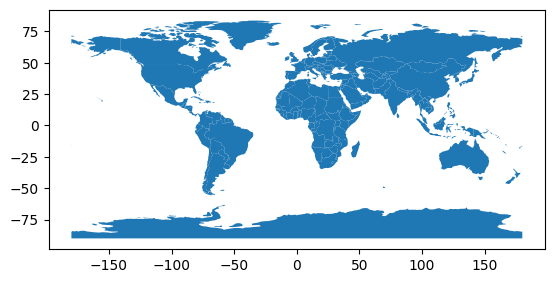
\includegraphics{labs/w01_intro_files/figure-pdf/cell-66-output-1.png}

We observe that:

\begin{itemize}
\tightlist
\item
  Using \texttt{.head()} we can see the first rows of the dataset, just
  like we can do with Pandas.
\item
  There is a \texttt{geometry} column and the different countries are
  represented as polygons
\item
  We can use the \texttt{.plot()} (matplotlib) method to quickly get a
  \emph{basic} visualization of the data
\end{itemize}

\subsection{What's a GeoDataFrame?}\label{whats-a-geodataframe}

We used the GeoPandas library to read in the geospatial data, and this
returned us a \texttt{GeoDataFrame}:

\begin{Shaded}
\begin{Highlighting}[]
\BuiltInTok{type}\NormalTok{(countries)}
\end{Highlighting}
\end{Shaded}

\begin{verbatim}
geopandas.geodataframe.GeoDataFrame
\end{verbatim}

A GeoDataFrame contains a tabular, geospatial dataset:

\begin{itemize}
\tightlist
\item
  It has a `geometry' column that holds the geometry information (or
  features in GeoJSON).
\item
  The other columns are the \textbf{attributes} (or properties in
  GeoJSON) that describe each of the geometries.
\end{itemize}

Such a \texttt{GeoDataFrame} is just like a pandas \texttt{DataFrame},
but with some additional functionality for working with geospatial data:
* A \texttt{geometry} attribute that always returns the column with the
geometry information (returning a \texttt{GeoSeries}). The column name
itself does not necessarily need to be `geometry', but it will always be
accessible as the \texttt{geometry} attribute. * It has some extra
methods for working with spatial data (area, distance, buffer,
intersection, \ldots)
\href{https://github.com/jorisvandenbossche/geopandas-tutorial/blob/main/04-spatial-operations-overlays.ipynb}{see
here, for example}.

\begin{Shaded}
\begin{Highlighting}[]
\NormalTok{countries.geometry.head()}
\end{Highlighting}
\end{Shaded}

\begin{verbatim}
0    POLYGON ((61.21082 35.65007, 62.23065 35.27066...
1    MULTIPOLYGON (((23.90415 -11.72228, 24.07991 -...
2    POLYGON ((21.02004 40.84273, 20.99999 40.58000...
3    POLYGON ((51.57952 24.24550, 51.75744 24.29407...
4    MULTIPOLYGON (((-66.95992 -54.89681, -67.56244...
Name: geometry, dtype: geometry
\end{verbatim}

\begin{Shaded}
\begin{Highlighting}[]
\BuiltInTok{type}\NormalTok{(countries.geometry)}
\end{Highlighting}
\end{Shaded}

\begin{verbatim}
geopandas.geoseries.GeoSeries
\end{verbatim}

\begin{Shaded}
\begin{Highlighting}[]
\NormalTok{countries.geometry.area}
\end{Highlighting}
\end{Shaded}

\begin{verbatim}
C:\Users\gfilo\AppData\Local\Temp\ipykernel_9708\3077649407.py:1: UserWarning: Geometry is in a geographic CRS. Results from 'area' are likely incorrect. Use 'GeoSeries.to_crs()' to re-project geometries to a projected CRS before this operation.

  countries.geometry.area
\end{verbatim}

\begin{verbatim}
0       63.593500
1      103.599439
2        3.185163
3        7.095047
4      278.923392
          ...    
172      0.631326
173     38.475618
174    112.718524
175     62.789498
176     32.280371
Length: 177, dtype: float64
\end{verbatim}

It's still a \texttt{DataFrame}, so we have all the \texttt{pandas}
functionality available to use on the geospatial dataset, and to do data
manipulations with the attributes and geometry information together. For
example, we can calculate the average population over all countries (by
accessing the `pop\_est' column, and calling the \texttt{mean} method on
it):

\begin{Shaded}
\begin{Highlighting}[]
\NormalTok{countries[}\StringTok{\textquotesingle{}pop\_est\textquotesingle{}}\NormalTok{].mean()}
\end{Highlighting}
\end{Shaded}

\begin{verbatim}
41712369.84180791
\end{verbatim}

\begin{Shaded}
\begin{Highlighting}[]
\NormalTok{africa }\OperatorTok{=}\NormalTok{ countries[countries[}\StringTok{\textquotesingle{}continent\textquotesingle{}}\NormalTok{] }\OperatorTok{==} \StringTok{\textquotesingle{}Africa\textquotesingle{}}\NormalTok{]}
\end{Highlighting}
\end{Shaded}

\begin{Shaded}
\begin{Highlighting}[]
\NormalTok{africa.plot()}\OperatorTok{;}
\end{Highlighting}
\end{Shaded}

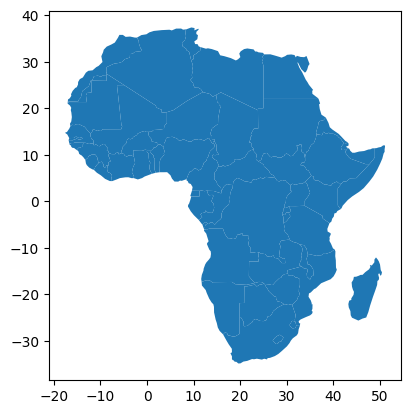
\includegraphics{labs/w01_intro_files/figure-pdf/cell-73-output-1.png}

The rest of the tutorial is going to assume you already know some pandas
basics, but we will try to give hints for that part for those that are
not familiar.

\textbf{Important:}

\begin{itemize}
\tightlist
\item
  A \texttt{GeoDataFrame} allows to perform typical tabular data
  analysis together with spatial operations
\item
  A \texttt{GeoDataFrame} (or \emph{Feature Collection}) consists of:

  \begin{itemize}
  \tightlist
  \item
    \textbf{Geometries} or \textbf{features}: the spatial objects
  \item
    \textbf{Attributes} or \textbf{properties}: columns with information
    about each spatial object
  \end{itemize}
\end{itemize}

\subsection{Geometries: Points, Linestrings and
Polygons}\label{geometries-points-linestrings-and-polygons}

Spatial \textbf{vector} data can consist of different types, and the 3
fundamental types are:

\begin{itemize}
\tightlist
\item
  \textbf{Point} data: represents a single point in space.
\item
  \textbf{Line} data (``LineString''): represents a sequence of points
  that form a line.
\item
  \textbf{Polygon} data: represents a filled area.
\end{itemize}

And each of them can also be combined in multi-part geometries (See
https://shapely.readthedocs.io/en/stable/manual.html\#geometric-objects
for extensive overview).

For the example we have seen up to now, the individual geometry objects
are Polygons:

\begin{Shaded}
\begin{Highlighting}[]
\BuiltInTok{print}\NormalTok{(countries.geometry[}\DecValTok{2}\NormalTok{])}
\end{Highlighting}
\end{Shaded}

\begin{verbatim}
POLYGON ((21.0200403174764 40.84272695572588, 20.999989861747224 40.58000397395401, 20.674996779063633 40.43499990494303, 20.615000441172754 40.11000682225935, 20.15001590341052 39.62499766698397, 19.980000441170148 39.69499339452341, 19.960001661873207 39.91500580500605, 19.406081984136733 40.250773423822466, 19.319058872157143 40.72723012955356, 19.40354983895429 41.40956574153546, 19.540027296637106 41.71998607031276, 19.37176883309496 41.877547512370654, 19.37176816334725 41.877550679783496, 19.304486118250793 42.19574514420782, 19.73805138517963 42.68824738216557, 19.801613396898688 42.50009349219084, 20.070700000000045 42.58863000000008, 20.283754510181893 42.32025950781508, 20.522950000000037 42.21787000000006, 20.590246546680227 41.855408919283626, 20.59024743010491 41.855404161133606, 20.463175083099202 41.51508901627534, 20.605181919037364 41.086226304685226, 21.0200403174764 40.84272695572588))
\end{verbatim}

Let's import some other datasets with different types of geometry
objects.

A dateset about cities in the world (adapted from
http://www.naturalearthdata.com/downloads/110m-cultural-vectors/110m-populated-places/,
zip file is available in the \texttt{/data} directory), consisting of
\texttt{Point} data:

\begin{Shaded}
\begin{Highlighting}[]
\NormalTok{cities }\OperatorTok{=}\NormalTok{ gpd.read\_file(}\StringTok{"../data/ne\_cities.zip"}\NormalTok{)}
\end{Highlighting}
\end{Shaded}

\begin{Shaded}
\begin{Highlighting}[]
\BuiltInTok{print}\NormalTok{(cities.geometry[}\DecValTok{0}\NormalTok{])}
\end{Highlighting}
\end{Shaded}

\begin{verbatim}
POINT (12.453386544971766 41.903282179960115)
\end{verbatim}

And a dataset of rivers in the world (from
http://www.naturalearthdata.com/downloads/50m-physical-vectors/50m-rivers-lake-centerlines/,
zip file is available in the \texttt{/data} directory) where each river
is a \texttt{(Multi-)LineString}:

\begin{Shaded}
\begin{Highlighting}[]
\NormalTok{rivers }\OperatorTok{=}\NormalTok{ gpd.read\_file(}\StringTok{"../data/ne\_rivers.zip"}\NormalTok{)}
\end{Highlighting}
\end{Shaded}

\begin{Shaded}
\begin{Highlighting}[]
\BuiltInTok{print}\NormalTok{(rivers.geometry[}\DecValTok{0}\NormalTok{])}
\end{Highlighting}
\end{Shaded}

\begin{verbatim}
LINESTRING (51.9371337598152 55.70106609892139, 51.880866467313695 55.68625891701544, 51.82031249962222 55.697455145538584, 51.747601827462404 55.69366250841807, 51.6628417966117 55.608172918745254, 51.57871093775964 55.59943268477065, 51.51342773400279 55.58312409100404, 51.508544921610905 55.52948639548083, 51.48583984403365 55.49640534033426, 51.36914062543957 55.46796295772435, 51.213062548697735 55.50264985760492, 51.13452148447897 55.48273346527725, 51.079345702742046 55.46759674659262, 50.98022460947817 55.46637604371949, 50.83445217522774 55.45630956063775, 50.6883789060617 55.42011139502489, 50.4118652342932 55.401190496444315, 50.07802734358711 55.381122137576654, 49.822167968676865 55.334662176818085, 49.53222656260584 55.260614325191, 49.38232421848795 55.17182037990665, 49.24808475131027 55.11301870345045)
\end{verbatim}

\subsection{\texorpdfstring{The \texttt{shapely}
library}{The shapely library}}\label{the-shapely-library}

The individual geometry objects are provided by the
\href{https://shapely.readthedocs.io/en/stable/}{\texttt{shapely}}
library

\begin{Shaded}
\begin{Highlighting}[]
\ImportTok{from}\NormalTok{ shapely.geometry }\ImportTok{import}\NormalTok{ Point, Polygon, LineString}
\end{Highlighting}
\end{Shaded}

\begin{Shaded}
\begin{Highlighting}[]
\BuiltInTok{type}\NormalTok{(countries.geometry[}\DecValTok{0}\NormalTok{])}
\end{Highlighting}
\end{Shaded}

\begin{verbatim}
shapely.geometry.polygon.Polygon
\end{verbatim}

To construct one ourselves:

\begin{Shaded}
\begin{Highlighting}[]
\NormalTok{p }\OperatorTok{=}\NormalTok{ Point(}\DecValTok{0}\NormalTok{, }\DecValTok{0}\NormalTok{)}
\end{Highlighting}
\end{Shaded}

\begin{Shaded}
\begin{Highlighting}[]
\BuiltInTok{print}\NormalTok{(p)}
\end{Highlighting}
\end{Shaded}

\begin{verbatim}
POINT (0 0)
\end{verbatim}

\begin{Shaded}
\begin{Highlighting}[]
\NormalTok{polygon }\OperatorTok{=}\NormalTok{ Polygon([(}\DecValTok{1}\NormalTok{, }\DecValTok{1}\NormalTok{), (}\DecValTok{2}\NormalTok{,}\DecValTok{2}\NormalTok{), (}\DecValTok{2}\NormalTok{, }\DecValTok{1}\NormalTok{)])}
\end{Highlighting}
\end{Shaded}

\begin{Shaded}
\begin{Highlighting}[]
\NormalTok{polygon.area}
\end{Highlighting}
\end{Shaded}

\begin{verbatim}
0.5
\end{verbatim}

\begin{Shaded}
\begin{Highlighting}[]
\NormalTok{polygon.distance(p)}
\end{Highlighting}
\end{Shaded}

\begin{verbatim}
1.4142135623730951
\end{verbatim}

\textbf{Important}:

Single geometries are represented by \texttt{shapely} objects:

\begin{itemize}
\tightlist
\item
  If you access a single geometry of a GeoDataFrame, you get a shapely
  geometry object
\item
  Those objects have similar functionality as geopandas objects
  (GeoDataFrame/GeoSeries). For example:

  \begin{itemize}
  \tightlist
  \item
    \texttt{single\_shapely\_object.distance(other\_point)}
    -\textgreater{} distance between two points
  \item
    \texttt{geodataframe.distance(other\_point)} -\textgreater{}
    distance for each point in the geodataframe to the other point
  \end{itemize}
\end{itemize}

\subsection{Plotting}\label{plotting}

\begin{Shaded}
\begin{Highlighting}[]
\OperatorTok{\%}\NormalTok{matplotlib inline}
\ImportTok{import}\NormalTok{ matplotlib}
\ImportTok{import}\NormalTok{ matplotlib.pyplot }\ImportTok{as}\NormalTok{ plt}

\NormalTok{fig, ax }\OperatorTok{=}\NormalTok{ plt.subplots(}\DecValTok{1}\NormalTok{, }\DecValTok{1}\NormalTok{, figsize}\OperatorTok{=}\NormalTok{(}\DecValTok{15}\NormalTok{, }\DecValTok{10}\NormalTok{))}
\NormalTok{countries.plot(ax }\OperatorTok{=}\NormalTok{ ax, edgecolor}\OperatorTok{=}\StringTok{\textquotesingle{}k\textquotesingle{}}\NormalTok{, facecolor}\OperatorTok{=}\StringTok{\textquotesingle{}none\textquotesingle{}}\NormalTok{)}
\NormalTok{rivers.plot(ax}\OperatorTok{=}\NormalTok{ax)}
\NormalTok{cities.plot(ax}\OperatorTok{=}\NormalTok{ax, color}\OperatorTok{=}\StringTok{\textquotesingle{}red\textquotesingle{}}\NormalTok{)}
\NormalTok{ax.}\BuiltInTok{set}\NormalTok{(xlim}\OperatorTok{=}\NormalTok{(}\OperatorTok{{-}}\DecValTok{20}\NormalTok{, }\DecValTok{60}\NormalTok{), ylim}\OperatorTok{=}\NormalTok{(}\OperatorTok{{-}}\DecValTok{40}\NormalTok{, }\DecValTok{40}\NormalTok{))}
\end{Highlighting}
\end{Shaded}

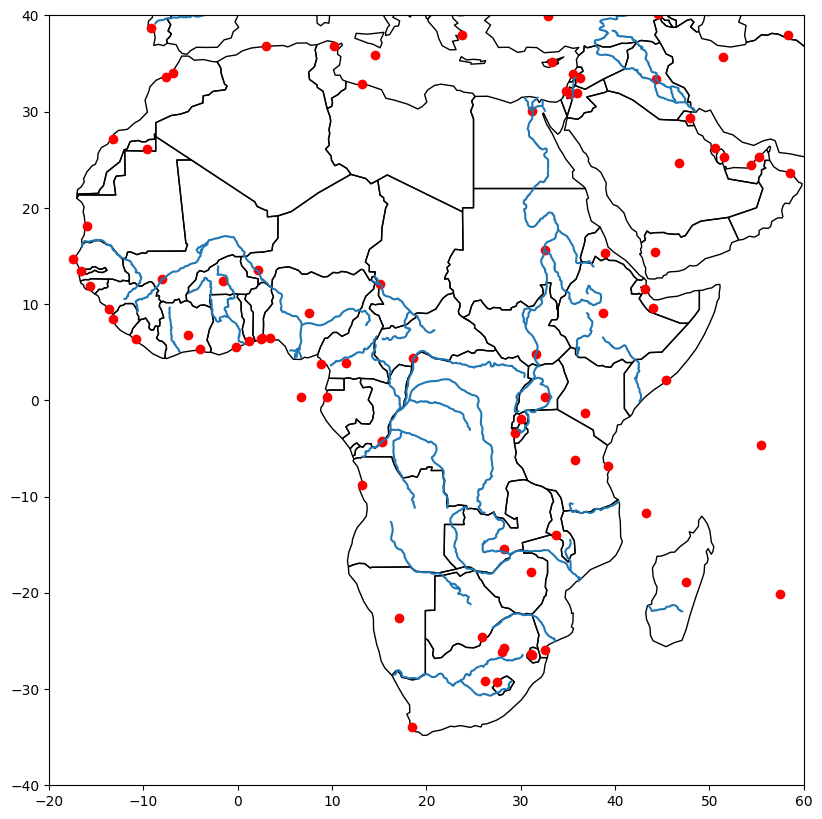
\includegraphics{labs/w01_intro_files/figure-pdf/cell-86-output-1.png}

\subsection{Creating GeoDataFrames (withouth specifying the
CRS)}\label{creating-geodataframes-withouth-specifying-the-crs}

\begin{Shaded}
\begin{Highlighting}[]
\NormalTok{gpd.GeoDataFrame(\{}
    \StringTok{\textquotesingle{}geometry\textquotesingle{}}\NormalTok{: [Point(}\DecValTok{1}\NormalTok{, }\DecValTok{1}\NormalTok{), Point(}\DecValTok{2}\NormalTok{, }\DecValTok{2}\NormalTok{)],}
    \StringTok{\textquotesingle{}attribute1\textquotesingle{}}\NormalTok{: [}\DecValTok{1}\NormalTok{, }\DecValTok{2}\NormalTok{],}
    \StringTok{\textquotesingle{}attribute2\textquotesingle{}}\NormalTok{: [}\FloatTok{0.1}\NormalTok{, }\FloatTok{0.2}\NormalTok{]\})}
\end{Highlighting}
\end{Shaded}

\begin{longtable}[]{@{}llll@{}}
\toprule\noalign{}
& geometry & attribute1 & attribute2 \\
\midrule\noalign{}
\endhead
\bottomrule\noalign{}
\endlastfoot
0 & POINT (1.00000 1.00000) & 1 & 0.1 \\
1 & POINT (2.00000 2.00000) & 2 & 0.2 \\
\end{longtable}

\begin{Shaded}
\begin{Highlighting}[]
\CommentTok{\# Creating a GeoDataFrame from an existing dataframe}
\CommentTok{\# For example, if you have lat/lon coordinates in two columns:}
\NormalTok{df }\OperatorTok{=}\NormalTok{ pd.DataFrame(}
\NormalTok{    \{}\StringTok{\textquotesingle{}City\textquotesingle{}}\NormalTok{: [}\StringTok{\textquotesingle{}Buenos Aires\textquotesingle{}}\NormalTok{, }\StringTok{\textquotesingle{}Brasilia\textquotesingle{}}\NormalTok{, }\StringTok{\textquotesingle{}Santiago\textquotesingle{}}\NormalTok{, }\StringTok{\textquotesingle{}Bogota\textquotesingle{}}\NormalTok{, }\StringTok{\textquotesingle{}Caracas\textquotesingle{}}\NormalTok{],}
     \StringTok{\textquotesingle{}Country\textquotesingle{}}\NormalTok{: [}\StringTok{\textquotesingle{}Argentina\textquotesingle{}}\NormalTok{, }\StringTok{\textquotesingle{}Brazil\textquotesingle{}}\NormalTok{, }\StringTok{\textquotesingle{}Chile\textquotesingle{}}\NormalTok{, }\StringTok{\textquotesingle{}Colombia\textquotesingle{}}\NormalTok{, }\StringTok{\textquotesingle{}Venezuela\textquotesingle{}}\NormalTok{],}
     \StringTok{\textquotesingle{}Latitude\textquotesingle{}}\NormalTok{: [}\OperatorTok{{-}}\FloatTok{34.58}\NormalTok{, }\OperatorTok{{-}}\FloatTok{15.78}\NormalTok{, }\OperatorTok{{-}}\FloatTok{33.45}\NormalTok{, }\FloatTok{4.60}\NormalTok{, }\FloatTok{10.48}\NormalTok{],}
     \StringTok{\textquotesingle{}Longitude\textquotesingle{}}\NormalTok{: [}\OperatorTok{{-}}\FloatTok{58.66}\NormalTok{, }\OperatorTok{{-}}\FloatTok{47.91}\NormalTok{, }\OperatorTok{{-}}\FloatTok{70.66}\NormalTok{, }\OperatorTok{{-}}\FloatTok{74.08}\NormalTok{, }\OperatorTok{{-}}\FloatTok{66.86}\NormalTok{]\})}
\end{Highlighting}
\end{Shaded}

\begin{Shaded}
\begin{Highlighting}[]
\NormalTok{gdf }\OperatorTok{=}\NormalTok{ gpd.GeoDataFrame(df, geometry}\OperatorTok{=}\NormalTok{gpd.points\_from\_xy(df.Longitude, df.Latitude))}
\NormalTok{gdf}
\end{Highlighting}
\end{Shaded}

\begin{longtable}[]{@{}llllll@{}}
\toprule\noalign{}
& City & Country & Latitude & Longitude & geometry \\
\midrule\noalign{}
\endhead
\bottomrule\noalign{}
\endlastfoot
0 & Buenos Aires & Argentina & -34.58 & -58.66 & POINT (-58.66000
-34.58000) \\
1 & Brasilia & Brazil & -15.78 & -47.91 & POINT (-47.91000 -15.78000) \\
2 & Santiago & Chile & -33.45 & -70.66 & POINT (-70.66000 -33.45000) \\
3 & Bogota & Colombia & 4.60 & -74.08 & POINT (-74.08000 4.60000) \\
4 & Caracas & Venezuela & 10.48 & -66.86 & POINT (-66.86000 10.48000) \\
\end{longtable}

\bookmarksetup{startatroot}

\chapter{Practice}\label{practice}

Throughout the exercises in this course, we will work with several
datasets about the city of Paris.

Here, we start with the following datasets:

\begin{itemize}
\tightlist
\item
  The administrative districts of Paris
  (https://opendata.paris.fr/explore/dataset/quartier\_paris/):
  \texttt{paris\_districts\_utm.geojson}
\item
  Real-time (at the moment I downloaded them ..) information about the
  public bicycle sharing system in Paris (vélib,
  https://opendata.paris.fr/explore/dataset/stations-velib-disponibilites-en-temps-reel/information/):
  \texttt{data/paris\_bike\_stations\_mercator.gpkg}
\end{itemize}

Both datasets are provided as spatial datasets using a GIS file format.

\textbf{Excercise 1}:

We will start with exploring the bicycle station dataset (available as a
GeoPackage file: \texttt{data/paris\_bike\_stations\_mercator.gpkg})

\begin{itemize}
\tightlist
\item
  Read the stations datasets into a GeoDataFrame called
  \texttt{stations}.
\item
  Check the type of the returned object
\item
  Check the first rows of the dataframes. What kind of geometries does
  this datasets contain?
\item
  How many features are there in the dataset?
\end{itemize}

Hints

\begin{itemize}
\tightlist
\item
  Use \texttt{type(..)} to check any Python object type
\item
  The \texttt{gpd.read\_file()} function can read different geospatial
  file formats. You pass the file name as first argument.
\item
  Use the \texttt{.shape} attribute to get the number of features
\end{itemize}

\textbf{Exercise 2}:

\begin{itemize}
\tightlist
\item
  Make a quick plot of the \texttt{stations} dataset.
\item
  Make the plot a bit larger by setting the figure size to (12, 6)
  (hint: the \texttt{plot} method accepts a \texttt{figsize} keyword).
\end{itemize}

\textbf{Exercise 3}:

Next, we will explore the dataset on the administrative districts of
Paris (available as a GeoJSON file:
``../data/paris\_districts\_utm.geojson'')

\begin{itemize}
\tightlist
\item
  Read the dataset into a GeoDataFrame called \texttt{districts}.
\item
  Check the first rows of the dataframe. What kind of geometries does
  this dataset contain?
\item
  How many features are there in the dataset? (hint: use the
  \texttt{.shape} attribute)
\item
  Make a quick plot of the \texttt{districts} dataset (set the figure
  size to (12, 6)).
\end{itemize}

\textbf{Exercise 4}:

What are the largest districts (biggest area)?

\begin{itemize}
\tightlist
\item
  Calculate the area of each district.
\item
  Add this area as a new column to the \texttt{districts} dataframe.
\item
  Sort the dataframe by this area column for largest to smallest values
  (descending).
\end{itemize}

Hints

\begin{itemize}
\tightlist
\item
  Adding a column can be done by assigning values to a column using the
  same square brackets syntax:
  \texttt{df{[}\textquotesingle{}new\_col\textquotesingle{}{]}\ =\ values}
\item
  To sort the rows of a DataFrame, use the \texttt{sort\_values()}
  method, specifying the colum to sort on with the
  \texttt{by=\textquotesingle{}col\_name\textquotesingle{}} keyword.
  Check the help of this method to see how to sort ascending or
  descending.
\end{itemize}

\section{Part IV: Coordinate reference systems \&
Projections}\label{part-iv-coordinate-reference-systems-projections}

\emph{Gabriele Filomena has prepared this notebook by readapting
material shared on this
\href{https://github.com/jorisvandenbossche/geopandas-tutorial}{repository}.
Copyright (c) 2018, Joris Van den Bossche.}

\begin{Shaded}
\begin{Highlighting}[]
\NormalTok{countries }\OperatorTok{=}\NormalTok{ gpd.read\_file(}\StringTok{"../data/ne\_countries.zip"}\NormalTok{)}
\NormalTok{cities }\OperatorTok{=}\NormalTok{ gpd.read\_file(}\StringTok{"../data/ne\_cities.zip"}\NormalTok{)}
\NormalTok{rivers }\OperatorTok{=}\NormalTok{ gpd.read\_file(}\StringTok{"../data/ne\_rivers.zip"}\NormalTok{)}
\end{Highlighting}
\end{Shaded}

\subsection{Coordinate reference
systems}\label{coordinate-reference-systems}

Up to now, we have used the geometry data with certain coordinates
without further wondering what those coordinates mean or how they are
expressed.

\begin{quote}
The \textbf{Coordinate Reference System (CRS)} relates the coordinates
to a specific location on earth.
\end{quote}

For an in-depth explanation, see
https://docs.qgis.org/2.8/en/docs/gentle\_gis\_introduction/coordinate\_reference\_systems.html

\subsubsection{Geographic coordinates}\label{geographic-coordinates}

\begin{quote}
Degrees of latitude and longitude.

E.g. 48°51′N, 2°17′E
\end{quote}

The most known type of coordinates are geographic coordinates: we define
a position on the globe in degrees of latitude and longitude, relative
to the equator and the prime meridian. With this system, we can easily
specify any location on earth. It is used widely, for example in GPS. If
you inspect the coordinates of a location in Google Maps, you will also
see latitude and longitude.

\textbf{Attention!}

in Python we use (lon, lat) and not (lat, lon)

\begin{itemize}
\tightlist
\item
  Longitude: {[}-180, 180{]}\{\{1\}\}
\item
  Latitude: {[}-90, 90{]}\{\{1\}\}
\end{itemize}

\subsection{Projected coordinates}\label{projected-coordinates}

\begin{quote}
\texttt{(x,\ y)} coordinates are usually in meters or feet
\end{quote}

Although the earth is a globe, in practice we usually represent it on a
flat surface: think about a physical map, or the figures we have made
with Python on our computer screen. Going from the globe to a flat map
is what we call a \emph{projection}.

We project the surface of the earth onto a 2D plane so we can express
locations in cartesian x and y coordinates, on a flat surface. In this
plane, we then typically work with a length unit such as meters instead
of degrees, which makes the analysis more convenient and effective.

However, there is an important remark: the 3 dimensional earth can never
be represented perfectly on a 2 dimensional map, so projections
inevitably introduce distortions. To minimize such errors, there are
different approaches to project, each with specific advantages and
disadvantages.

Some projection systems will try to preserve the area size of
geometries, such as the Albers Equal Area projection. Other projection
systems try to preserve angles, such as the Mercator projection, but
will see big distortions in the area. Every projection system will
always have some distortion of area, angle or distance.

\textbf{Projected size vs actual size (Mercator projection)}:

\subsection{Coordinate Reference Systems in Python /
GeoPandas}\label{coordinate-reference-systems-in-python-geopandas}

A GeoDataFrame or GeoSeries has a \texttt{.crs} attribute which holds
(optionally) a description of the coordinate reference system of the
geometries:

\begin{Shaded}
\begin{Highlighting}[]
\NormalTok{countries.crs}
\end{Highlighting}
\end{Shaded}

\begin{verbatim}
<Geographic 2D CRS: EPSG:4326>
Name: WGS 84
Axis Info [ellipsoidal]:
- Lat[north]: Geodetic latitude (degree)
- Lon[east]: Geodetic longitude (degree)
Area of Use:
- name: World.
- bounds: (-180.0, -90.0, 180.0, 90.0)
Datum: World Geodetic System 1984 ensemble
- Ellipsoid: WGS 84
- Prime Meridian: Greenwich
\end{verbatim}

For the \texttt{countries} dataframe, it indicates that it uses the EPSG
4326 / WGS84 lon/lat reference system, which is one of the most used for
geographic coordinates.

It uses coordinates as latitude and longitude in degrees, as can you be
seen from the x/y labels on the plot:

\begin{Shaded}
\begin{Highlighting}[]
\NormalTok{countries.plot()}
\end{Highlighting}
\end{Shaded}

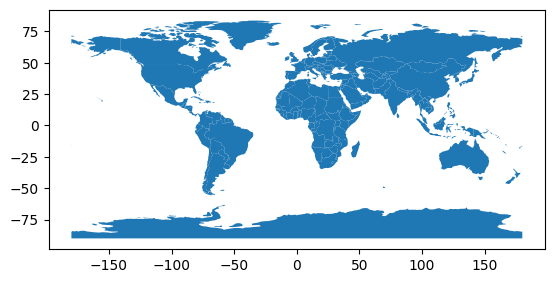
\includegraphics{labs/w01_intro_files/figure-pdf/cell-102-output-1.png}

The \texttt{.crs} attribute returns a \texttt{pyproj.CRS} object. To
specify a CRS, we typically use some string representation:

\begin{itemize}
\tightlist
\item
  \textbf{EPSG code} Example: \texttt{EPSG:4326} = WGS84 geographic CRS
  (longitude, latitude)
\end{itemize}

For more information, see also
http://geopandas.readthedocs.io/en/latest/projections.html.

\subsubsection{Transforming to another
CRS}\label{transforming-to-another-crs}

We can convert a GeoDataFrame to another reference system using the
\texttt{to\_crs} function.

For example, let's convert the countries to the World Mercator
projection (http://epsg.io/3395):

\begin{Shaded}
\begin{Highlighting}[]
\CommentTok{\# remove Antartica, as the Mercator projection cannot deal with the poles}
\NormalTok{countries }\OperatorTok{=}\NormalTok{ countries[(countries[}\StringTok{\textquotesingle{}name\textquotesingle{}}\NormalTok{] }\OperatorTok{!=} \StringTok{"Antarctica"}\NormalTok{)]}
\NormalTok{countries\_mercator }\OperatorTok{=}\NormalTok{ countries.to\_crs(epsg}\OperatorTok{=}\DecValTok{3395}\NormalTok{)  }\CommentTok{\# or .to\_crs("EPSG:3395")}
\NormalTok{countries\_mercator.plot()}
\end{Highlighting}
\end{Shaded}

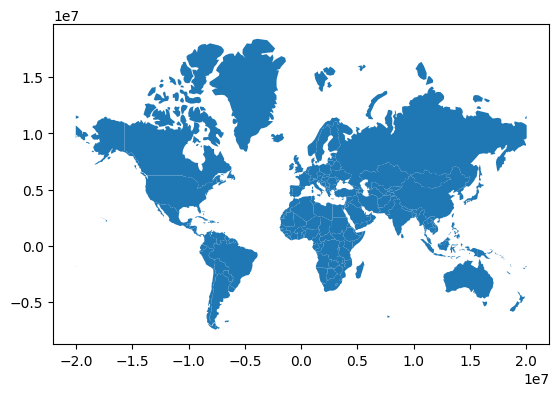
\includegraphics{labs/w01_intro_files/figure-pdf/cell-103-output-1.png}

Note the different scale of x and y.

\subsubsection{Why using a different
CRS?}\label{why-using-a-different-crs}

There are sometimes good reasons you want to change the coordinate
references system of your dataset, for example:

\begin{itemize}
\tightlist
\item
  Different sources with different CRS -\textgreater{} need to convert
  to the same crs.\\
\item
  Different countries/geographical areas with different CRS.
\item
  Mapping (distortion of shape and distances).
\item
  Distance / area based calculations -\textgreater{} ensure you use an
  appropriate projected coordinate system expressed in a meaningful unit
  such as meters or feet (\textbf{not degrees!}).
\end{itemize}

\textbf{Important:}

All the calculations (e.g.~distance, spatial operations, etc.) that
happen in \texttt{GeoPandas} and \texttt{Shapely} assume that your data
is in a 2D cartesian plane, and thus the result of those calculations
will only be correct if your data is properly projected.

\section{Practice}\label{practice-1}

Again, we will go back to the Paris datasets. Up to now, we provided the
datasets in an appropriate projected CRS for the exercises. But the
original data were actually using geographic coordinates. In the
following exercises, we will start from there.

Going back to the Paris districts dataset, this is now provided as a
GeoJSON file (\texttt{"../data/paris\_districts.geojson"}) in geographic
coordinates.

For converting to projected coordinates, we will use the standard
projected CRS for France is the RGF93 / Lambert-93 reference system,
referenced by the \texttt{EPSG:2154} number.

\textbf{Exercise: Projecting a GeoDataFrame}

\begin{itemize}
\tightlist
\item
  Read the districts datasets
  (\texttt{../data/paris\_districts.geojson"}) into a GeoDataFrame
  called \texttt{districts}.
\item
  Look at the CRS attribute of the GeoDataFrame. Do you recognize the
  EPSG number?
\item
  Make a plot of the \texttt{districts} dataset.
\item
  Calculate the area of all districts.
\item
  Convert the \texttt{districts} to a projected CRS (using the
  \texttt{EPSG:2154} for France). Call the new dataset
  \texttt{districts\_RGF93}.
\item
  Make a similar plot of \texttt{districts\_RGF93}.
\item
  Calculate the area of all districts again with
  \texttt{districts\_RGF93} (the result will now be expressed in m²).
\end{itemize}

Hints

\begin{itemize}
\tightlist
\item
  The CRS information is stored in the \texttt{.crs} attribute of a
  GeoDataFrame.
\item
  Making a simple plot of a GeoDataFrame can be done with the
  \texttt{.plot()} method.
\item
  Converting to a different CRS can be done with the \texttt{.to\_crs()}
  method, and the CRS can be specified as an EPSG number using the
  \texttt{epsg} keyword.
\end{itemize}

\bookmarksetup{startatroot}

\chapter{Static Maps in Python}\label{static-maps-in-python}

The \textbf{Lecture slides} can be found
\href{https://github.com/GDSL-UL/wma/raw/main/html/w02.html}{here}.

\section{Part I: Basic Maps}\label{part-i-basic-maps}

In this session, we will use the libraries \texttt{matplotlib} and
\texttt{contextily} to plot the information represented into different
\texttt{GeoDataFrames}. We will look into plotting \texttt{Point},
\texttt{LineString} and \texttt{Polygon} \texttt{GeoDataFrames}. Most of
the plots here are rather ugly but, at this point, the goal is to get
familiar with the parameters of the plot function and what can be done
with them.

\begin{Shaded}
\begin{Highlighting}[]
\OperatorTok{\%}\NormalTok{matplotlib inline}
\ImportTok{import}\NormalTok{ matplotlib}
\ImportTok{import}\NormalTok{ matplotlib.pyplot }\ImportTok{as}\NormalTok{ plt}
\ImportTok{import}\NormalTok{ geopandas }\ImportTok{as}\NormalTok{ gpd}
\ImportTok{import}\NormalTok{ pandas }\ImportTok{as}\NormalTok{ pd}
\ImportTok{import}\NormalTok{ osmnx }\ImportTok{as}\NormalTok{ ox}
\ImportTok{import}\NormalTok{ contextily }\ImportTok{as}\NormalTok{ ctx}
\ImportTok{import}\NormalTok{ seaborn }\ImportTok{as}\NormalTok{ sns}
\end{Highlighting}
\end{Shaded}

\subsection{Plotting Points}\label{plotting-points}

Load the data of terrorist attacks 1970-2020 and choose a country.
Germany is used as a case study here but feel free to change the
country. If you do so, also change the \texttt{crs} (see
https://epsg.io).

\begin{Shaded}
\begin{Highlighting}[]
\NormalTok{attacks }\OperatorTok{=}\NormalTok{ pd.read\_csv(}\StringTok{"../data/GTD\_2022.csv"}\NormalTok{, low\_memory }\OperatorTok{=} \VariableTok{False}\NormalTok{)}
\end{Highlighting}
\end{Shaded}

Creating the \texttt{GeoDataFrame} from the \texttt{DataFrame}

\begin{Shaded}
\begin{Highlighting}[]
\NormalTok{germany }\OperatorTok{=}\NormalTok{ [}\StringTok{\textquotesingle{}West Germany (FRG)\textquotesingle{}}\NormalTok{, }\StringTok{\textquotesingle{}Germany\textquotesingle{}}\NormalTok{, }\StringTok{\textquotesingle{}East Germany (GDR)\textquotesingle{}}\NormalTok{] }\CommentTok{\# Germany was split till 1989 in two entities}
\NormalTok{df }\OperatorTok{=}\NormalTok{ attacks[attacks.country\_txt.isin(germany)].copy()}

\CommentTok{\# Uncomment the lines below for other countries that haven\textquotesingle{}t changed their denominations/boundaries between 1970 and today:}
\CommentTok{\# country = \textquotesingle{}France\textquotesingle{} }
\CommentTok{\# df = attacks[attacks.country\_txt == country].copy()\#}
\NormalTok{wgs }\OperatorTok{=} \StringTok{\textquotesingle{}EPSG:4326\textquotesingle{}}
\NormalTok{germany\_crs }\OperatorTok{=} \StringTok{\textquotesingle{}EPSG:4839\textquotesingle{}}
\NormalTok{gdf }\OperatorTok{=}\NormalTok{ gpd.GeoDataFrame(df, geometry}\OperatorTok{=}\NormalTok{gpd.points\_from\_xy(df.longitude, df.latitude), crs }\OperatorTok{=}\NormalTok{ wgs)}
\NormalTok{gdf }\OperatorTok{=}\NormalTok{ gdf[}\OperatorTok{\textasciitilde{}}\NormalTok{gdf.geometry.is\_empty] }\CommentTok{\# remove empty geometries}
\NormalTok{gdf.to\_file(}\StringTok{"../data/germany.shp"}\NormalTok{)}
\NormalTok{gdf }\OperatorTok{=}\NormalTok{ gdf.to\_crs(germany\_crs)}
\end{Highlighting}
\end{Shaded}

\begin{verbatim}
C:\Users\gfilo\AppData\Local\Temp\ipykernel_700\3815068564.py:11: UserWarning: Column names longer than 10 characters will be truncated when saved to ESRI Shapefile.
  gdf.to_file("data/germany.shp")
\end{verbatim}

Basic plotting

\begin{Shaded}
\begin{Highlighting}[]
\CommentTok{\# prepare the axis and coordinate}
\NormalTok{nr\_rows }\OperatorTok{=} \DecValTok{1}
\NormalTok{nr\_cols }\OperatorTok{=} \DecValTok{1}
\NormalTok{fig, ax }\OperatorTok{=}\NormalTok{ plt.subplots(nr\_cols, nr\_rows, figsize}\OperatorTok{=}\NormalTok{(}\DecValTok{8}\NormalTok{, }\DecValTok{6}\NormalTok{))}
\NormalTok{gdf.plot(ax}\OperatorTok{=}\NormalTok{ax, color}\OperatorTok{=}\StringTok{\textquotesingle{}red\textquotesingle{}}\NormalTok{, markersize}\OperatorTok{=}\DecValTok{7}\NormalTok{)}
\end{Highlighting}
\end{Shaded}

\includegraphics{labs/w02_maps_files/figure-pdf/cell-5-output-1.png}

Slightly improving the plot:

\begin{Shaded}
\begin{Highlighting}[]
\CommentTok{\# removing ticks}
\NormalTok{ax.xaxis.set\_ticklabels([])}
\NormalTok{ax.yaxis.set\_ticklabels([])}
\NormalTok{ax.tick\_params(axis}\OperatorTok{=} \StringTok{\textquotesingle{}both\textquotesingle{}}\NormalTok{, which}\OperatorTok{=} \StringTok{\textquotesingle{}both\textquotesingle{}}\NormalTok{, length}\OperatorTok{=}\DecValTok{0}\NormalTok{)}
\NormalTok{title\_parameters }\OperatorTok{=}\NormalTok{ \{}\StringTok{\textquotesingle{}fontsize\textquotesingle{}}\NormalTok{:}\StringTok{\textquotesingle{}16\textquotesingle{}}\NormalTok{, }\StringTok{\textquotesingle{}fontname\textquotesingle{}}\NormalTok{:}\StringTok{\textquotesingle{}Times New Roman\textquotesingle{}}\NormalTok{\}}
\NormalTok{ax.set\_title(}\StringTok{"Terroristic Attacks in Germany"}\NormalTok{, }\OperatorTok{**}\NormalTok{title\_parameters)}
\NormalTok{fig}
\end{Highlighting}
\end{Shaded}

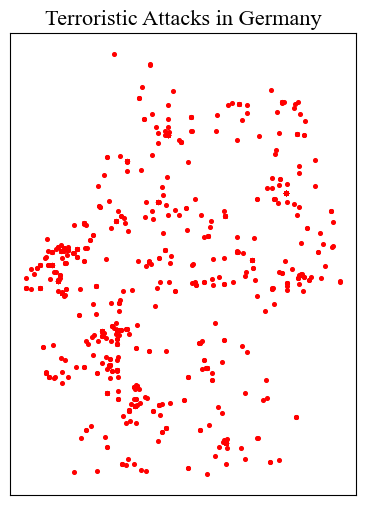
\includegraphics{labs/w02_maps_files/figure-pdf/cell-6-output-1.png}

\subsubsection{\texorpdfstring{Adding some context: Base Maps with
\texttt{Contextily}}{Adding some context: Base Maps with Contextily}}\label{adding-some-context-base-maps-with-contextily}

see providers and options here
https://xyzservices.readthedocs.io/en/stable/introduction.html

\begin{Shaded}
\begin{Highlighting}[]
\NormalTok{source }\OperatorTok{=}\NormalTok{ ctx.providers.CartoDB.Positron}
\NormalTok{ctx.add\_basemap(ax, crs}\OperatorTok{=}\NormalTok{ gdf.crs.to\_string(), source}\OperatorTok{=}\NormalTok{ source)}
\CommentTok{\# replot}
\NormalTok{fig}
\end{Highlighting}
\end{Shaded}

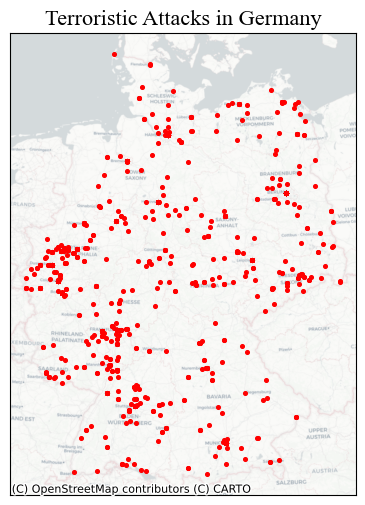
\includegraphics{labs/w02_maps_files/figure-pdf/cell-7-output-1.png}

\begin{verbatim}
<Figure size 640x480 with 0 Axes>
\end{verbatim}

\subsubsection{\texorpdfstring{Parameters specific to \texttt{Point} in
the \texttt{plot}
method}{Parameters specific to Point in the plot method}}\label{parameters-specific-to-point-in-the-plot-method}

\begin{itemize}
\tightlist
\item
  \texttt{markersize}: numerical value (for now)
\item
  \texttt{marker}: see
  https://matplotlib.org/stable/api/markers\_api.html
\end{itemize}

\paragraph{Other properties, shape
independent:}\label{other-properties-shape-independent}

\begin{itemize}
\tightlist
\item
  \texttt{color}:
  https://matplotlib.org/3.1.0/gallery/color/named\_colors.html
\item
  \texttt{alpha}: regulates transparency of the shape: 0 to 1
\end{itemize}

\begin{Shaded}
\begin{Highlighting}[]
\CommentTok{\# first, let\textquotesingle{}s make a function}

\KeywordTok{def}\NormalTok{ ax\_ticks\_off(ax):}
\NormalTok{    ax.xaxis.set\_ticklabels([])}
\NormalTok{    ax.yaxis.set\_ticklabels([])}
\NormalTok{    ax.tick\_params(axis}\OperatorTok{=} \StringTok{\textquotesingle{}both\textquotesingle{}}\NormalTok{, which}\OperatorTok{=} \StringTok{\textquotesingle{}both\textquotesingle{}}\NormalTok{, length}\OperatorTok{=}\DecValTok{0}\NormalTok{)}
\end{Highlighting}
\end{Shaded}

\begin{Shaded}
\begin{Highlighting}[]
\CommentTok{\# prepare the axis and coordinate}
\NormalTok{fig, ax }\OperatorTok{=}\NormalTok{ plt.subplots(}\DecValTok{1}\NormalTok{, }\DecValTok{1}\NormalTok{, figsize}\OperatorTok{=}\NormalTok{(}\DecValTok{8}\NormalTok{, }\DecValTok{6}\NormalTok{))}
\NormalTok{gdf.plot(ax}\OperatorTok{=}\NormalTok{ax, markersize }\OperatorTok{=} \DecValTok{15}\NormalTok{, color }\OperatorTok{=} \StringTok{\textquotesingle{}blue\textquotesingle{}}\NormalTok{, marker }\OperatorTok{=} \StringTok{\textquotesingle{}*\textquotesingle{}}\NormalTok{, alpha }\OperatorTok{=} \FloatTok{0.3}\NormalTok{)}
\NormalTok{ctx.add\_basemap(ax, crs}\OperatorTok{=}\NormalTok{ gdf.crs.to\_string(), source}\OperatorTok{=}\NormalTok{ source)}
\NormalTok{ax\_ticks\_off(ax)}
\end{Highlighting}
\end{Shaded}

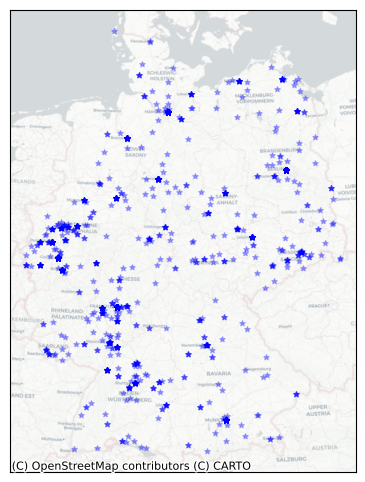
\includegraphics{labs/w02_maps_files/figure-pdf/cell-9-output-1.png}

\subsection{Plotting LineStrings}\label{plotting-linestrings}

Let's import railway tracks in the Western Balkans (Slovenia, Croatia,
Bosnia \& Herzegovina, Montenegro, Serbia, Kosovo)

\begin{Shaded}
\begin{Highlighting}[]
\NormalTok{wb\_crs }\OperatorTok{=} \StringTok{\textquotesingle{}EPSG:31277\textquotesingle{}}
\NormalTok{lines\_gdf }\OperatorTok{=}\NormalTok{ gpd.read\_file(}\StringTok{"..\textbackslash{}data\textbackslash{}wb\_railways.shp"}\NormalTok{)}
\NormalTok{lines\_gdf.plot()}
\end{Highlighting}
\end{Shaded}

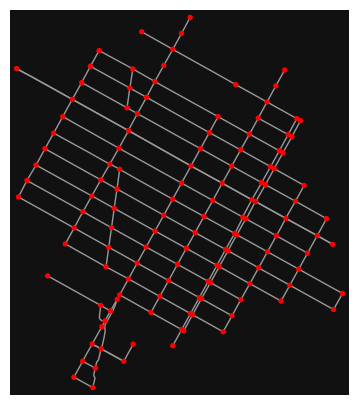
\includegraphics{labs/w02_maps_files/figure-pdf/cell-10-output-1.png}

\begin{Shaded}
\begin{Highlighting}[]
\CommentTok{\# prepare the plot}
\NormalTok{fig, ax }\OperatorTok{=}\NormalTok{ plt.subplots(}\DecValTok{1}\NormalTok{, }\DecValTok{1}\NormalTok{, figsize}\OperatorTok{=}\NormalTok{(}\DecValTok{8}\NormalTok{, }\DecValTok{6}\NormalTok{))}
\NormalTok{lines\_gdf.plot(ax}\OperatorTok{=}\NormalTok{ax, linewidth }\OperatorTok{=} \FloatTok{0.8}\NormalTok{, color }\OperatorTok{=} \StringTok{\textquotesingle{}blue\textquotesingle{}}\NormalTok{, alpha }\OperatorTok{=} \DecValTok{1}\NormalTok{)}
\NormalTok{ctx.add\_basemap(ax, crs}\OperatorTok{=}\NormalTok{ lines\_gdf.crs.to\_string(), source }\OperatorTok{=}\NormalTok{ ctx.providers.Esri.WorldGrayCanvas)}
\NormalTok{ax\_ticks\_off(ax)}
\NormalTok{ax.set\_title(}\StringTok{"Railway infrastructure in the West Balkans"}\NormalTok{, }\OperatorTok{**}\NormalTok{title\_parameters) }\CommentTok{\#parameters as above}
\end{Highlighting}
\end{Shaded}

\begin{verbatim}
Text(0.5, 1.0, 'Railway infrastructure in the West Balkans')
\end{verbatim}

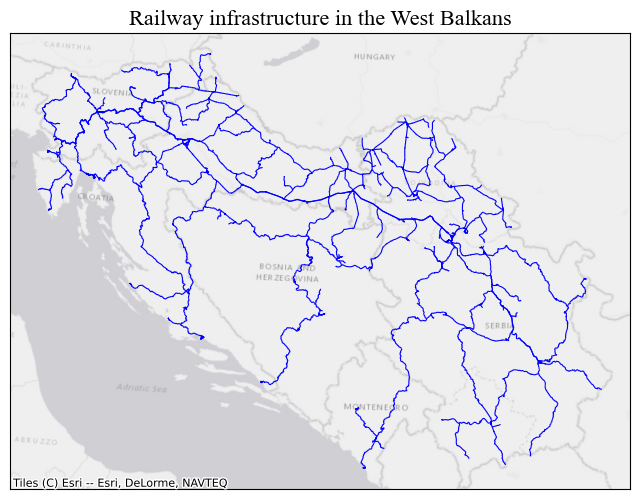
\includegraphics{labs/w02_maps_files/figure-pdf/cell-11-output-2.png}

One can also filter prior to plotting, based on the columns in the
GeoDataFrame. First we download Serbia's Boundary with \texttt{OSMNX},
more on that later on. Then we filter \texttt{lines\_gdf} with a
\texttt{within} operation.

\begin{Shaded}
\begin{Highlighting}[]
\NormalTok{serbia }\OperatorTok{=}\NormalTok{ ox.geocode\_to\_gdf(}\StringTok{\textquotesingle{}Serbia\textquotesingle{}}\NormalTok{)}
\NormalTok{serbia }\OperatorTok{=}\NormalTok{ serbia.to\_crs(wb\_crs)}
\NormalTok{serbia\_lines }\OperatorTok{=}\NormalTok{ lines\_gdf[lines\_gdf.geometry.within(serbia.iloc[}\DecValTok{0}\NormalTok{].geometry)].copy() }\CommentTok{\#there\textquotesingle{}s only one polygon in the gdf}
\end{Highlighting}
\end{Shaded}

\begin{Shaded}
\begin{Highlighting}[]
\CommentTok{\# prepare the plot}
\NormalTok{fig, ax }\OperatorTok{=}\NormalTok{ plt.subplots(}\DecValTok{1}\NormalTok{, }\DecValTok{1}\NormalTok{, figsize}\OperatorTok{=}\NormalTok{(}\DecValTok{8}\NormalTok{, }\DecValTok{6}\NormalTok{))}
\NormalTok{serbia\_lines.plot(ax}\OperatorTok{=}\NormalTok{ax, linewidth }\OperatorTok{=} \FloatTok{0.8}\NormalTok{, color }\OperatorTok{=} \StringTok{\textquotesingle{}blue\textquotesingle{}}\NormalTok{, alpha }\OperatorTok{=} \DecValTok{1}\NormalTok{)}
\NormalTok{ctx.add\_basemap(ax, crs}\OperatorTok{=}\NormalTok{ lines\_gdf.crs.to\_string(), source }\OperatorTok{=}\NormalTok{ ctx.providers.Esri.WorldGrayCanvas)}
\NormalTok{ax\_ticks\_off(ax)}
\NormalTok{ax.set\_title(}\StringTok{"Railway infrastructure in Serbia and Kosovo"}\NormalTok{, }\OperatorTok{**}\NormalTok{title\_parameters) }\CommentTok{\#parameters as above}
\end{Highlighting}
\end{Shaded}

\begin{verbatim}
Text(0.5, 1.0, 'Railway infrastructure in Serbia and Kosovo')
\end{verbatim}

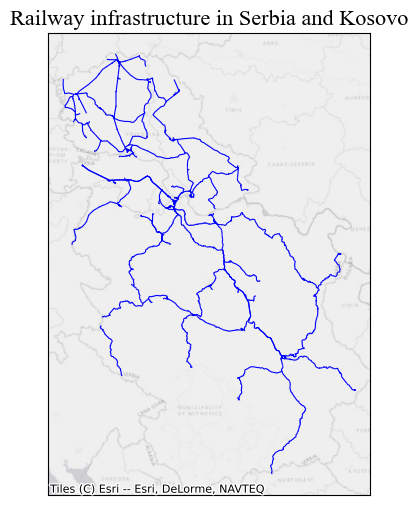
\includegraphics{labs/w02_maps_files/figure-pdf/cell-13-output-2.png}

\subsubsection{\texorpdfstring{Parameters specific to
\texttt{LineString}:}{Parameters specific to LineString:}}\label{parameters-specific-to-linestring}

\begin{itemize}
\tightlist
\item
  \texttt{linewidth}: numerical value (for now).
\item
  \texttt{capstyle}: controls how Matplotlib draws the corners where two
  different line segments meet. See
  https://matplotlib.org/stable/gallery/lines\_bars\_and\_markers/capstyle.html
\item
  \texttt{joinstyle}': controls how Matplotlib draws the corners where
  two different line segments meet.
  https://matplotlib.org/stable/gallery/lines\_bars\_and\_markers/joinstyle.html
\end{itemize}

\begin{Shaded}
\begin{Highlighting}[]
\CommentTok{\# prepare the plot}
\NormalTok{fig, ax }\OperatorTok{=}\NormalTok{ plt.subplots(}\DecValTok{1}\NormalTok{, }\DecValTok{1}\NormalTok{, figsize}\OperatorTok{=}\NormalTok{(}\DecValTok{10}\NormalTok{, }\DecValTok{10}\NormalTok{))}
\NormalTok{serbia\_lines.plot(ax}\OperatorTok{=}\NormalTok{ax, linewidth }\OperatorTok{=} \FloatTok{0.9}\NormalTok{, color }\OperatorTok{=} \StringTok{\textquotesingle{}black\textquotesingle{}}\NormalTok{, alpha }\OperatorTok{=} \DecValTok{1}\NormalTok{, capstyle }\OperatorTok{=} \StringTok{\textquotesingle{}round\textquotesingle{}}\NormalTok{, joinstyle }\OperatorTok{=} \StringTok{\textquotesingle{}round\textquotesingle{}}\NormalTok{)}
\NormalTok{ax.set\_axis\_off() }\CommentTok{\# we don\textquotesingle{}t need the ticks function}
\NormalTok{ax.set\_title(}\StringTok{"Railway infrastructure in Serbia"}\NormalTok{, }\OperatorTok{**}\NormalTok{title\_parameters) }\CommentTok{\#parameters as above}
\end{Highlighting}
\end{Shaded}

\begin{verbatim}
Text(0.5, 1.0, 'Railway infrastructure in Serbia')
\end{verbatim}

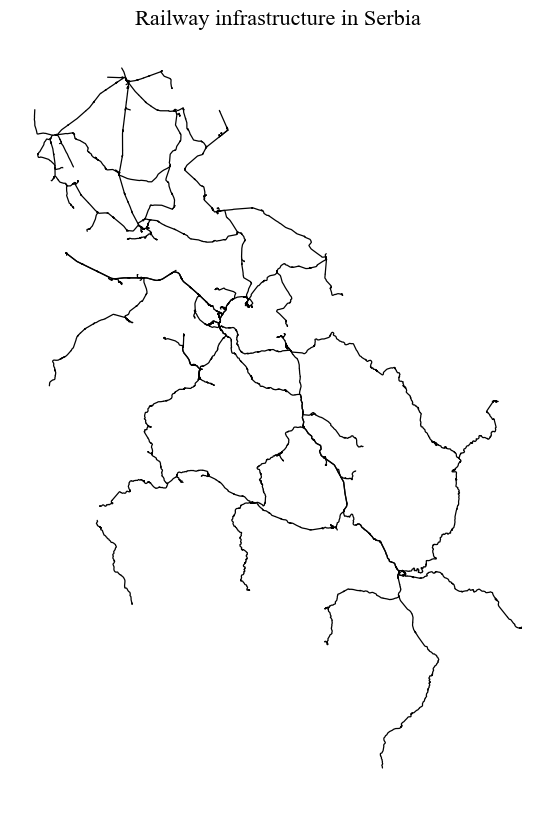
\includegraphics{labs/w02_maps_files/figure-pdf/cell-14-output-2.png}

\subsection{Plotting Polygons}\label{plotting-polygons}

We are again using \texttt{OSMNX} to download data from
\texttt{OpenStreetMap} automatically. In this case, we will get building
footprints from the city of Algiers in Alageria.

\subsubsection{\texorpdfstring{Parameter specific to
\texttt{Polygon}:}{Parameter specific to Polygon:}}\label{parameter-specific-to-polygon}

\begin{itemize}
\tightlist
\item
  \texttt{edgecolor}: the outline of the polygon, by default =
  \texttt{None} (often better).
\item
  \texttt{linewidth}: the width of the outline of the polygon.
\end{itemize}

\begin{Shaded}
\begin{Highlighting}[]
\NormalTok{algeria\_crs }\OperatorTok{=} \StringTok{\textquotesingle{}EPSG:30729\textquotesingle{}}
\NormalTok{tags }\OperatorTok{=}\NormalTok{ \{}\StringTok{"building"}\NormalTok{: }\VariableTok{True}\NormalTok{\} }\CommentTok{\#OSM tags}
\NormalTok{buildings }\OperatorTok{=}\NormalTok{ ox.features\_from\_address(}\StringTok{"Algiers, Algeria"}\NormalTok{, tags }\OperatorTok{=}\NormalTok{ tags, dist }\OperatorTok{=} \DecValTok{2000}\NormalTok{) }
\NormalTok{buildings }\OperatorTok{=}\NormalTok{ buildings.reset\_index()}
 \CommentTok{\# sometimes building footprints are represented by Points, let\textquotesingle{}s disregard them}
\NormalTok{buildings }\OperatorTok{=}\NormalTok{ buildings[(buildings.geometry.geom\_type }\OperatorTok{==} \StringTok{\textquotesingle{}Polygon\textquotesingle{}}\NormalTok{) }\OperatorTok{|}\NormalTok{ (buildings.geometry.geom\_type }\OperatorTok{==} \StringTok{\textquotesingle{}MultiPolygon\textquotesingle{}}\NormalTok{)]}
\NormalTok{buildings }\OperatorTok{=}\NormalTok{ buildings.to\_crs(algeria\_crs)}
\end{Highlighting}
\end{Shaded}

\begin{Shaded}
\begin{Highlighting}[]
\NormalTok{fig, ax }\OperatorTok{=}\NormalTok{ plt.subplots(}\DecValTok{1}\NormalTok{, }\DecValTok{1}\NormalTok{, figsize}\OperatorTok{=}\NormalTok{(}\DecValTok{15}\NormalTok{, }\DecValTok{10}\NormalTok{))}
\NormalTok{ax.set\_title(}\StringTok{"Buildings in Algiers"}\NormalTok{, }\OperatorTok{**}\NormalTok{title\_parameters)}
\NormalTok{ax.set\_axis\_off() }\CommentTok{\# we don\textquotesingle{}t need the ticks function}
\NormalTok{buildings.plot(ax}\OperatorTok{=}\NormalTok{ax, color }\OperatorTok{=} \StringTok{\textquotesingle{}orange\textquotesingle{}}\NormalTok{, edgecolor }\OperatorTok{=} \StringTok{\textquotesingle{}black\textquotesingle{}}\NormalTok{, lw }\OperatorTok{=} \FloatTok{0.2}\NormalTok{)}
\NormalTok{source }\OperatorTok{=}\NormalTok{ ctx.providers.CartoDB.PositronNoLabels}
\NormalTok{ctx.add\_basemap(ax, crs}\OperatorTok{=}\NormalTok{ buildings.crs.to\_string(), source}\OperatorTok{=}\NormalTok{ source)}
\end{Highlighting}
\end{Shaded}

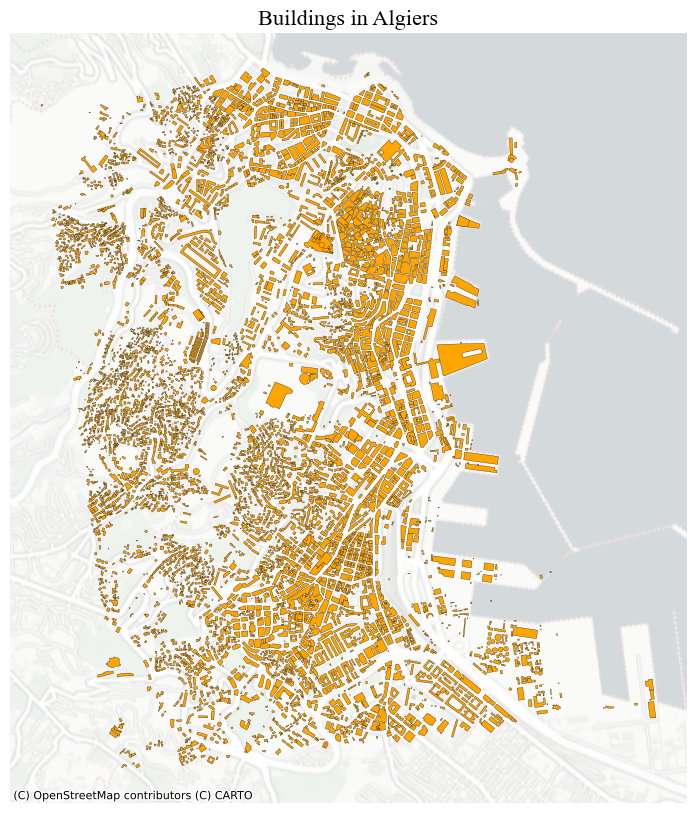
\includegraphics{labs/w02_maps_files/figure-pdf/cell-16-output-1.png}

For polygons, you can also plot just the boundaries of the geometries
by:

\begin{Shaded}
\begin{Highlighting}[]
\NormalTok{buildings.boundary.plot(lw }\OperatorTok{=} \FloatTok{0.5}\NormalTok{)}
\end{Highlighting}
\end{Shaded}

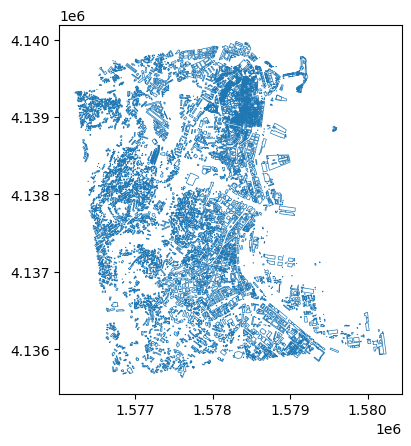
\includegraphics{labs/w02_maps_files/figure-pdf/cell-17-output-1.png}

\subsection{Plotting more than one layer
together}\label{plotting-more-than-one-layer-together}

Let's also download roads for Algiers

\begin{Shaded}
\begin{Highlighting}[]
\NormalTok{tags }\OperatorTok{=}\NormalTok{ \{}\StringTok{"highway"}\NormalTok{: }\VariableTok{True}\NormalTok{\} }\CommentTok{\#OSM tags}
\NormalTok{roads }\OperatorTok{=}\NormalTok{ ox.features\_from\_address(}\StringTok{"Algiers, Algeria"}\NormalTok{, tags }\OperatorTok{=}\NormalTok{ tags, dist }\OperatorTok{=} \DecValTok{2000}\NormalTok{) }
\NormalTok{roads }\OperatorTok{=}\NormalTok{ roads.reset\_index()}
\NormalTok{roads }\OperatorTok{=}\NormalTok{ roads.to\_crs(algeria\_crs)}
 \CommentTok{\# sometimes building footprints are represented by Points, let\textquotesingle{}s disregard them}
\NormalTok{roads }\OperatorTok{=}\NormalTok{ roads[roads.geometry.geom\_type }\OperatorTok{==} \StringTok{\textquotesingle{}LineString\textquotesingle{}}\NormalTok{]}
\end{Highlighting}
\end{Shaded}

And plot everything togehter. It's important to keep in mind that the
last layer is always rendered on top of the others. In other words, they
may cover the previous ones.

However, you can prevent this by passing arguments to the parameter
\texttt{zorder} in the \texttt{plot} method. The layer with the higher
zorder value will be plotted on top.

\begin{Shaded}
\begin{Highlighting}[]
\NormalTok{fig, ax }\OperatorTok{=}\NormalTok{ plt.subplots(}\DecValTok{1}\NormalTok{, }\DecValTok{1}\NormalTok{, figsize}\OperatorTok{=}\NormalTok{(}\DecValTok{15}\NormalTok{, }\DecValTok{10}\NormalTok{))}
\NormalTok{ax.set\_title(}\StringTok{"Buildings and Roads in Algiers"}\NormalTok{, }\OperatorTok{**}\NormalTok{title\_parameters)}
\NormalTok{ax.set\_axis\_off() }\CommentTok{\# we don\textquotesingle{}t need the ticks function}
\CommentTok{\# only roads within the extent of the buildings layer}
\NormalTok{roads[roads.geometry.within(buildings.unary\_union.envelope)].plot(ax}\OperatorTok{=}\NormalTok{ax, color }\OperatorTok{=} \StringTok{\textquotesingle{}grey\textquotesingle{}}\NormalTok{, lw }\OperatorTok{=} \FloatTok{0.5}\NormalTok{) }\CommentTok{\#linewidth can be also passed as lw }
\NormalTok{buildings.plot(ax}\OperatorTok{=}\NormalTok{ax, color }\OperatorTok{=} \StringTok{\textquotesingle{}orange\textquotesingle{}}\NormalTok{)}
\end{Highlighting}
\end{Shaded}

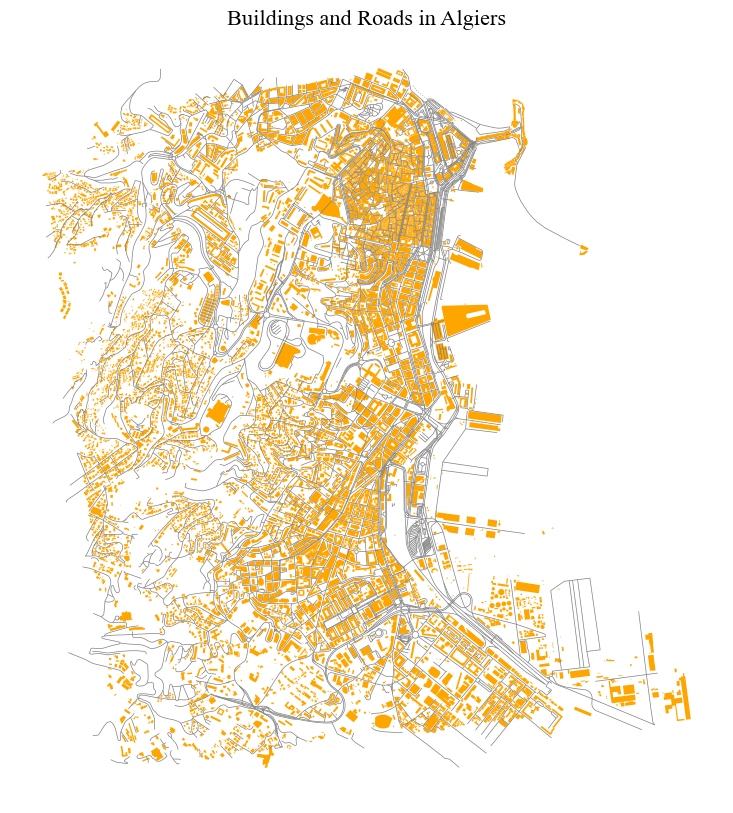
\includegraphics{labs/w02_maps_files/figure-pdf/cell-19-output-1.png}

\subsection{Sub-plots}\label{sub-plots}

To obtain multiple sub-plots, we manipulate the \texttt{nrows},
\texttt{ncols} parameters. We can use this approach to: * Plot the same
layer with different properties.

\begin{Shaded}
\begin{Highlighting}[]
\NormalTok{fig, axes }\OperatorTok{=}\NormalTok{ plt.subplots(}\DecValTok{1}\NormalTok{, }\DecValTok{2}\NormalTok{, figsize}\OperatorTok{=}\NormalTok{(}\DecValTok{10}\NormalTok{, }\DecValTok{6}\NormalTok{))}
\NormalTok{colors }\OperatorTok{=}\NormalTok{ [}\StringTok{\textquotesingle{}red\textquotesingle{}}\NormalTok{, }\StringTok{\textquotesingle{}blue\textquotesingle{}}\NormalTok{]}

\ControlFlowTok{for}\NormalTok{ n, ax }\KeywordTok{in} \BuiltInTok{enumerate}\NormalTok{(axes):}
\NormalTok{    gdf.plot(ax}\OperatorTok{=}\NormalTok{ax, markersize }\OperatorTok{=} \DecValTok{4}\NormalTok{, color }\OperatorTok{=}\NormalTok{ colors[n])}
\NormalTok{    ax.set\_axis\_off()}
\NormalTok{    ctx.add\_basemap(ax, crs}\OperatorTok{=}\NormalTok{ gdf.crs.to\_string(), source}\OperatorTok{=}\NormalTok{ source)}
\end{Highlighting}
\end{Shaded}

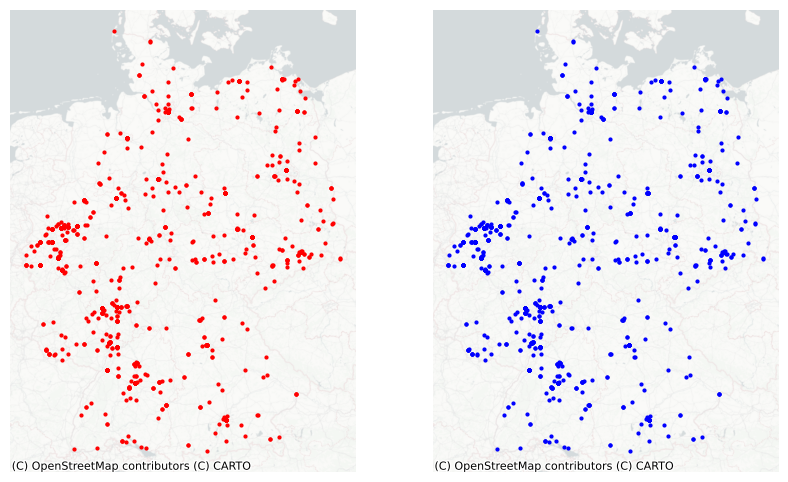
\includegraphics{labs/w02_maps_files/figure-pdf/cell-20-output-1.png}

\begin{itemize}
\tightlist
\item
  Plot different layers.
\end{itemize}

\begin{Shaded}
\begin{Highlighting}[]
\NormalTok{fig, axes }\OperatorTok{=}\NormalTok{ plt.subplots(}\DecValTok{1}\NormalTok{, }\DecValTok{2}\NormalTok{, figsize}\OperatorTok{=}\NormalTok{(}\DecValTok{10}\NormalTok{, }\DecValTok{6}\NormalTok{))}
\NormalTok{gdfs }\OperatorTok{=}\NormalTok{ [buildings, roads]}
\NormalTok{colors }\OperatorTok{=}\NormalTok{ [}\StringTok{\textquotesingle{}orange\textquotesingle{}}\NormalTok{, }\StringTok{\textquotesingle{}grey\textquotesingle{}}\NormalTok{]}

\NormalTok{buildings.plot(ax}\OperatorTok{=}\NormalTok{axes[}\DecValTok{0}\NormalTok{], color }\OperatorTok{=} \StringTok{\textquotesingle{}orange\textquotesingle{}}\NormalTok{, edgecolor }\OperatorTok{=} \StringTok{\textquotesingle{}none\textquotesingle{}}\NormalTok{)}
\NormalTok{roads.plot(ax}\OperatorTok{=}\NormalTok{axes[}\DecValTok{1}\NormalTok{], color }\OperatorTok{=} \StringTok{\textquotesingle{}gray\textquotesingle{}}\NormalTok{, lw }\OperatorTok{=} \FloatTok{0.5}\NormalTok{)}

\ControlFlowTok{for}\NormalTok{ ax }\KeywordTok{in}\NormalTok{ axes:}
\NormalTok{    ax.set\_axis\_off()}
\NormalTok{    ctx.add\_basemap(ax, crs}\OperatorTok{=}\NormalTok{ buildings.crs.to\_string(), source }\OperatorTok{=}\NormalTok{ source)}
\end{Highlighting}
\end{Shaded}

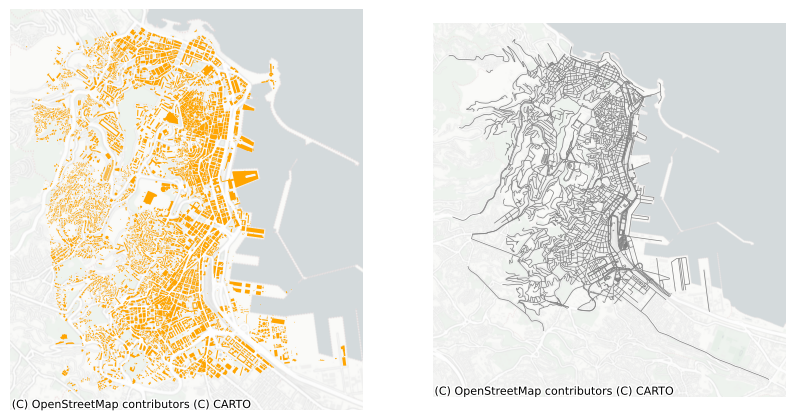
\includegraphics{labs/w02_maps_files/figure-pdf/cell-21-output-1.png}

\begin{itemize}
\tightlist
\item
  Analyse phenomena across different geographical areas. For example,
  terrorism in Germany and in the UK.
\end{itemize}

\begin{Shaded}
\begin{Highlighting}[]
\CommentTok{\# let\textquotesingle{}s prepare the gdf for the UK}
\NormalTok{df\_uk }\OperatorTok{=}\NormalTok{ attacks[attacks.country\_txt }\OperatorTok{==} \StringTok{\textquotesingle{}United Kingdom\textquotesingle{}}\NormalTok{].copy()}
\NormalTok{uk\_crs }\OperatorTok{=} \StringTok{\textquotesingle{}EPSG:27700\textquotesingle{}}
\NormalTok{gdf\_uk }\OperatorTok{=}\NormalTok{ gpd.GeoDataFrame(df\_uk, geometry}\OperatorTok{=}\NormalTok{gpd.points\_from\_xy(df\_uk.longitude, df\_uk.latitude), crs }\OperatorTok{=}\NormalTok{ wgs)}
\NormalTok{gdf\_uk }\OperatorTok{=}\NormalTok{ gdf\_uk.to\_crs(uk\_crs)}
\end{Highlighting}
\end{Shaded}

\begin{Shaded}
\begin{Highlighting}[]
\NormalTok{fig, axes }\OperatorTok{=}\NormalTok{ plt.subplots(}\DecValTok{1}\NormalTok{, }\DecValTok{2}\NormalTok{, figsize}\OperatorTok{=}\NormalTok{(}\DecValTok{10}\NormalTok{, }\DecValTok{6}\NormalTok{))}
\NormalTok{gdfs }\OperatorTok{=}\NormalTok{ [gdf, gdf\_uk]}

\ControlFlowTok{for}\NormalTok{ n, ax }\KeywordTok{in} \BuiltInTok{enumerate}\NormalTok{(axes):}
\NormalTok{    gdf\_tmp }\OperatorTok{=}\NormalTok{ gdfs[n]}
\NormalTok{    gdf\_tmp.plot(ax}\OperatorTok{=}\NormalTok{ax, color }\OperatorTok{=} \StringTok{\textquotesingle{}orange\textquotesingle{}}\NormalTok{, markersize }\OperatorTok{=} \DecValTok{3}\NormalTok{)}
\NormalTok{    ax.set\_axis\_off()}
\NormalTok{    ctx.add\_basemap(ax, crs}\OperatorTok{=}\NormalTok{ gdf\_tmp.crs.to\_string(), source}\OperatorTok{=}\NormalTok{ source)}
\end{Highlighting}
\end{Shaded}

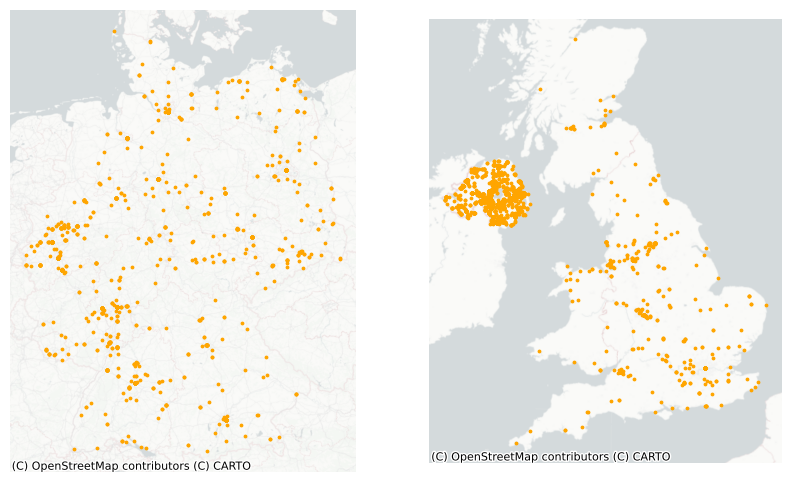
\includegraphics{labs/w02_maps_files/figure-pdf/cell-23-output-1.png}

\textbf{Exercise}:

\begin{itemize}
\tightlist
\item
  Think about the plots above and how they could be improved.
\item
  Copy and paste the code and execute the functions playing with the
  different parameters.
\item
  Produce a neat map using the GeoDataFrames avaible in this notebook or
  the ones employed in the previous sessions, making use of the
  elements/parameters discussed here.
\item
  Try out different tiles for the basemap to familiarise yourself with
  what's aveilable.
\end{itemize}

\section{Part II: Choropleth Mapping}\label{part-ii-choropleth-mapping}

\begin{Shaded}
\begin{Highlighting}[]
\ImportTok{import}\NormalTok{ geoplot.crs }\ImportTok{as}\NormalTok{ gcrs}
\ImportTok{import}\NormalTok{ geoplot }\ImportTok{as}\NormalTok{ gplt}
\end{Highlighting}
\end{Shaded}

\textbf{Data}

For this second part of the tutorial, we will use some data at the
municipality level for Serbia. The data contains information regarding
poverty level, average income, population and tourism. The data is taken
from https://data.stat.gov.rs/?caller=SDDB\&languageCode=en-US and can
be associated to the polygons representing the administrative boundaries
of the municipalities. These boundaries can be found here
https://data.humdata.org/dataset/geoboundaries-admin-boundaries-for-serbia?force\_layout=desktop.
While most of the data refers to 2023, the admin boundaries file traces
back to 2017. Thus, it may contain obsolete information (few changes may
occur).

Later on, we will go back to the terrorism dataset.

\begin{Shaded}
\begin{Highlighting}[]
\CommentTok{\# This will be different on your computer and will depend on where}
\CommentTok{\# you have downloaded the files}
\NormalTok{serbia\_crs }\OperatorTok{=} \StringTok{\textquotesingle{}EPSG:31277\textquotesingle{}}
\NormalTok{wgs }\OperatorTok{=} \StringTok{\textquotesingle{}EPSG:4326\textquotesingle{}}
\NormalTok{serbia\_admin }\OperatorTok{=}\NormalTok{ gpd.read\_file(}\StringTok{\textquotesingle{}../data/serbia\_admin.shp\textquotesingle{}}\NormalTok{)}
\NormalTok{serbia\_admin.set\_index(}\StringTok{\textquotesingle{}townID\textquotesingle{}}\NormalTok{, inplace }\OperatorTok{=} \VariableTok{True}\NormalTok{, drop }\OperatorTok{=} \VariableTok{True}\NormalTok{)}
\NormalTok{serbia\_admin }\OperatorTok{=}\NormalTok{ serbia\_admin.to\_crs(serbia\_crs)}
\end{Highlighting}
\end{Shaded}

Let's plot the \texttt{GeoDataFrame} following the last session's steps.

\begin{Shaded}
\begin{Highlighting}[]
\NormalTok{fig, ax }\OperatorTok{=}\NormalTok{ plt.subplots(}\DecValTok{1}\NormalTok{, }\DecValTok{1}\NormalTok{, figsize}\OperatorTok{=}\NormalTok{(}\DecValTok{8}\NormalTok{, }\DecValTok{6}\NormalTok{))}
\NormalTok{serbia\_admin.plot(ax }\OperatorTok{=}\NormalTok{ ax, color }\OperatorTok{=} \StringTok{\textquotesingle{}salmon\textquotesingle{}}\NormalTok{, linewidth }\OperatorTok{=} \FloatTok{0.3}\NormalTok{, edgecolor }\OperatorTok{=} \StringTok{\textquotesingle{}white\textquotesingle{}}\NormalTok{)}
\NormalTok{ax.set\_axis\_off()}
\NormalTok{title\_parameters }\OperatorTok{=}\NormalTok{ \{}\StringTok{\textquotesingle{}fontsize\textquotesingle{}}\NormalTok{:}\StringTok{\textquotesingle{}16\textquotesingle{}}\NormalTok{, }\StringTok{\textquotesingle{}fontname\textquotesingle{}}\NormalTok{:}\StringTok{\textquotesingle{}Times New Roman\textquotesingle{}}\NormalTok{\}}
\NormalTok{ax.set\_title(}\StringTok{"Serbian Municipalities"}\NormalTok{, }\OperatorTok{**}\NormalTok{title\_parameters) }\CommentTok{\#parameters as above}
\end{Highlighting}
\end{Shaded}

\begin{verbatim}
Text(0.5, 1.0, 'Serbian Municipalities')
\end{verbatim}

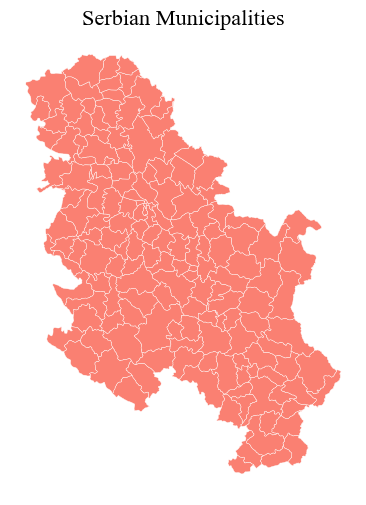
\includegraphics{labs/w02_maps_files/figure-pdf/cell-26-output-2.png}

The we load the data and merge it into the \texttt{GeoDataFrame}, before
getting rid of municipalities that do not have a corresponding
shape/record in the GeoDataFrame (probably the result of changes in the
national subdivisions).

\begin{Shaded}
\begin{Highlighting}[]
\NormalTok{data }\OperatorTok{=}\NormalTok{ pd.read\_csv(}\StringTok{"../data/serbia\_data.csv"}\NormalTok{) }\CommentTok{\#some slavic characters }
\NormalTok{data.drop(}\StringTok{\textquotesingle{}name\_en\textquotesingle{}}\NormalTok{, axis }\OperatorTok{=} \DecValTok{1}\NormalTok{, inplace }\OperatorTok{=} \VariableTok{True}\NormalTok{)}
\NormalTok{serbia\_admin }\OperatorTok{=}\NormalTok{ pd.merge(serbia\_admin, data, left\_on }\OperatorTok{=} \StringTok{"townID"}\NormalTok{, right\_on }\OperatorTok{=} \StringTok{"id"}\NormalTok{)}
\NormalTok{serbia\_admin }\OperatorTok{=}\NormalTok{ serbia\_admin[serbia\_admin.}\BuiltInTok{id}\NormalTok{.notna()]}
\NormalTok{serbia\_admin[}\StringTok{\textquotesingle{}id\textquotesingle{}}\NormalTok{] }\OperatorTok{=}\NormalTok{ serbia\_admin[}\StringTok{\textquotesingle{}id\textquotesingle{}}\NormalTok{].astype(}\StringTok{\textquotesingle{}int64\textquotesingle{}}\NormalTok{)}
\NormalTok{serbia\_admin.head()}

\CommentTok{\#let\textquotesingle{}s save the so{-}obtained gdf for later (encoding for dealing with slavic characters).}
\NormalTok{serbia\_admin.to\_file(}\StringTok{"../data/serbia\_data.shp"}\NormalTok{, encoding}\OperatorTok{=}\StringTok{\textquotesingle{}utf{-}8\textquotesingle{}}\NormalTok{)}
\end{Highlighting}
\end{Shaded}

Creating a choropleth map is rather straightforward and can ben done by
using few other parameters. Reflect on what you see and whether the map
below is informative.

\begin{Shaded}
\begin{Highlighting}[]
\NormalTok{fig, ax }\OperatorTok{=}\NormalTok{ plt.subplots(}\DecValTok{1}\NormalTok{, }\DecValTok{1}\NormalTok{, figsize}\OperatorTok{=}\NormalTok{(}\DecValTok{8}\NormalTok{, }\DecValTok{6}\NormalTok{))}
\NormalTok{serbia\_admin.plot(ax }\OperatorTok{=}\NormalTok{ ax, column }\OperatorTok{=} \StringTok{\textquotesingle{}gross\textquotesingle{}}\NormalTok{, linewidth }\OperatorTok{=} \FloatTok{0.3}\NormalTok{, cmap }\OperatorTok{=} \StringTok{\textquotesingle{}Greens\textquotesingle{}}\NormalTok{, legend }\OperatorTok{=} \VariableTok{True}\NormalTok{)}
\NormalTok{ax.set\_axis\_off()}
\NormalTok{title\_parameters }\OperatorTok{=}\NormalTok{ \{}\StringTok{\textquotesingle{}fontsize\textquotesingle{}}\NormalTok{:}\StringTok{\textquotesingle{}16\textquotesingle{}}\NormalTok{, }\StringTok{\textquotesingle{}fontname\textquotesingle{}}\NormalTok{:}\StringTok{\textquotesingle{}Times New Roman\textquotesingle{}}\NormalTok{\}}
\NormalTok{ax.set\_title(}\StringTok{"Serbian Municipalities"}\NormalTok{, }\OperatorTok{**}\NormalTok{title\_parameters) }\CommentTok{\#parameters as above}
\end{Highlighting}
\end{Shaded}

\begin{verbatim}
Text(0.5, 1.0, 'Serbian Municipalities')
\end{verbatim}

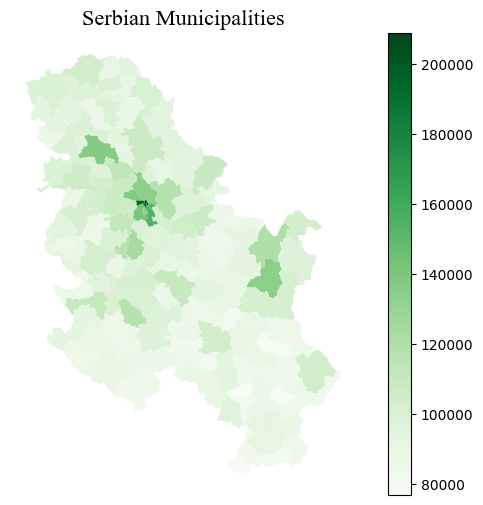
\includegraphics{labs/w02_maps_files/figure-pdf/cell-28-output-2.png}

\subsection{Choropleth Maps for Numerical
Variables}\label{choropleth-maps-for-numerical-variables}

We are essentialy using the same approach emplyed for creating basic
maps, the method \texttt{plot}, but we now need to pass arguments to
some new parameters to specify which column is to be represented and
how. As an optional argument, one can set legend to \texttt{True} and
the resulting figure will include a color bar.

\begin{itemize}
\tightlist
\item
  \texttt{column}: the name of the column representing the variable that
  we want to used to colour-code our shapes.
\item
  \texttt{scheme}: the scheme used to color the shapes based on the
  variable values.
\item
  \texttt{cmap}: the colormap used to show variation.
\end{itemize}

\subsubsection{Colormaps}\label{colormaps}

Built-in color maps can be found here
https://matplotlib.org/stable/gallery/color/colormap\_reference.html.
However one can create new ones as follows from a list of colours:

\begin{Shaded}
\begin{Highlighting}[]
\ImportTok{from}\NormalTok{ seaborn }\ImportTok{import}\NormalTok{ palplot}
\ImportTok{from}\NormalTok{ matplotlib.colors }\ImportTok{import}\NormalTok{ LinearSegmentedColormap}

\NormalTok{colors }\OperatorTok{=}\NormalTok{ [(}\FloatTok{0.00}\NormalTok{, }\FloatTok{0.00}\NormalTok{, }\FloatTok{0.00}\NormalTok{,}\DecValTok{1}\NormalTok{), (}\FloatTok{0.248}\NormalTok{, }\FloatTok{0.0271}\NormalTok{, }\FloatTok{0.569}\NormalTok{, }\DecValTok{1}\NormalTok{), (}\FloatTok{0.0311}\NormalTok{, }\FloatTok{0.258}\NormalTok{, }\FloatTok{0.646}\NormalTok{,}\DecValTok{1}\NormalTok{),}
\NormalTok{            (}\FloatTok{0.019}\NormalTok{, }\FloatTok{0.415}\NormalTok{, }\FloatTok{0.415}\NormalTok{,}\DecValTok{1}\NormalTok{), (}\FloatTok{0.025}\NormalTok{, }\FloatTok{0.538}\NormalTok{, }\FloatTok{0.269}\NormalTok{,}\DecValTok{1}\NormalTok{), (}\FloatTok{0.0315}\NormalTok{, }\FloatTok{0.658}\NormalTok{, }\FloatTok{0.103}\NormalTok{,}\DecValTok{1}\NormalTok{),}
\NormalTok{            (}\FloatTok{0.331}\NormalTok{, }\FloatTok{0.761}\NormalTok{, }\FloatTok{0.036}\NormalTok{,}\DecValTok{1}\NormalTok{),(}\FloatTok{0.768}\NormalTok{, }\FloatTok{0.809}\NormalTok{, }\FloatTok{0.039}\NormalTok{,}\DecValTok{1}\NormalTok{), (}\FloatTok{0.989}\NormalTok{, }\FloatTok{0.862}\NormalTok{, }\FloatTok{0.772}\NormalTok{,}\DecValTok{1}\NormalTok{),}
\NormalTok{            (}\FloatTok{1.0}\NormalTok{, }\FloatTok{1.0}\NormalTok{, }\FloatTok{1.0}\NormalTok{)]}
\NormalTok{palplot(colors)}
\end{Highlighting}
\end{Shaded}

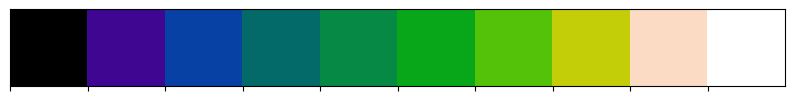
\includegraphics{labs/w02_maps_files/figure-pdf/cell-29-output-1.png}

\begin{Shaded}
\begin{Highlighting}[]
\NormalTok{kindlmann }\OperatorTok{=}\NormalTok{ LinearSegmentedColormap.from\_list(}\StringTok{\textquotesingle{}kindlmann\textquotesingle{}}\NormalTok{, colors)}
\end{Highlighting}
\end{Shaded}

or from color names:

\begin{Shaded}
\begin{Highlighting}[]
\NormalTok{colors }\OperatorTok{=}\NormalTok{ [}\StringTok{"white"}\NormalTok{, }\StringTok{"yellow"}\NormalTok{, }\StringTok{"red"}\NormalTok{]}
\NormalTok{palplot(colors)}
\end{Highlighting}
\end{Shaded}

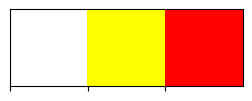
\includegraphics{labs/w02_maps_files/figure-pdf/cell-31-output-1.png}

Let's try a new colormap and let's also set a number of classes to
divide the data in, through the parameter \texttt{k}.

\begin{Shaded}
\begin{Highlighting}[]
\NormalTok{white\_to\_red }\OperatorTok{=}\NormalTok{ LinearSegmentedColormap.from\_list(}\StringTok{"name"}\NormalTok{, [}\StringTok{"yellow"}\NormalTok{,}\StringTok{"red"}\NormalTok{])}
\end{Highlighting}
\end{Shaded}

\begin{Shaded}
\begin{Highlighting}[]
\NormalTok{fig, ax }\OperatorTok{=}\NormalTok{ plt.subplots(}\DecValTok{1}\NormalTok{, }\DecValTok{1}\NormalTok{, figsize}\OperatorTok{=}\NormalTok{(}\DecValTok{8}\NormalTok{, }\DecValTok{6}\NormalTok{))}
\NormalTok{serbia\_admin.plot(ax }\OperatorTok{=}\NormalTok{ ax, column }\OperatorTok{=} \StringTok{\textquotesingle{}gross\textquotesingle{}}\NormalTok{, linewidth }\OperatorTok{=} \FloatTok{0.3}\NormalTok{, cmap }\OperatorTok{=}\NormalTok{ kindlmann.}\BuiltInTok{reversed}\NormalTok{(), legend }\OperatorTok{=} \VariableTok{True}\NormalTok{, k }\OperatorTok{=} \DecValTok{8}\NormalTok{)}
\NormalTok{ax.set\_axis\_off()}
\NormalTok{title\_parameters }\OperatorTok{=}\NormalTok{ \{}\StringTok{\textquotesingle{}fontsize\textquotesingle{}}\NormalTok{:}\StringTok{\textquotesingle{}16\textquotesingle{}}\NormalTok{, }\StringTok{\textquotesingle{}fontname\textquotesingle{}}\NormalTok{:}\StringTok{\textquotesingle{}Times New Roman\textquotesingle{}}\NormalTok{\}}
\NormalTok{ax.set\_title(}\StringTok{"Serbian Municipalities"}\NormalTok{, }\OperatorTok{**}\NormalTok{title\_parameters) }\CommentTok{\#parameters as above}
\end{Highlighting}
\end{Shaded}

\begin{verbatim}
Text(0.5, 1.0, 'Serbian Municipalities')
\end{verbatim}

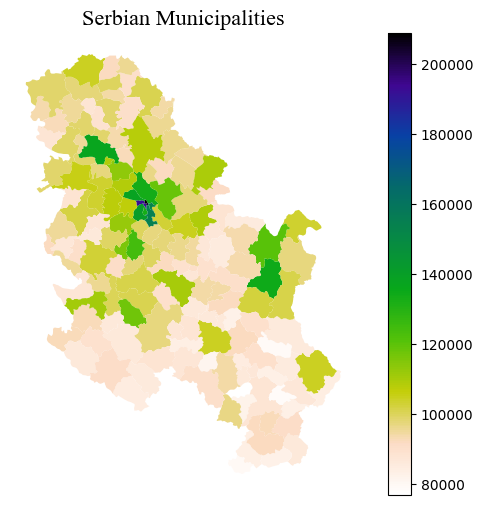
\includegraphics{labs/w02_maps_files/figure-pdf/cell-33-output-2.png}

With \texttt{GeoPandas}, when you use the \texttt{plot} method with
\texttt{legend=True} the type of legend that appears depends on the data
being visualized:

\begin{itemize}
\tightlist
\item
  Continuous Data: For columns with continuous data (like population
  estimates, temperatures, etc.), a color bar is generated as the
  legend. This color bar represents a range of values with a gradient,
  indicating how data values correspond to colors on the map.
\item
  Categorical Data: For columns with categorical data (like country
  names, types of land use, etc.), if you specify \texttt{legend=True},
  \texttt{GeoPandas} will try to create a legend that categorizes these
  distinct values with different colors. However, creating legends for
  categorical data is not as straightforward as with continuous data and
  might require additional handling for a clear and informative legend
  (see below).
\end{itemize}

\subsubsection{Scheme}\label{scheme}

It is important to keep in mind that choropleth maps strongly depend on
the scheme that it is passed (or the dafult one) to classify the data in
groups. The plot above only shows one municipality cooloured in dark
blue.

Look at the following plots and how three different classifiers produce
different results for the same data.

Refer to https://geopandas.org/en/stable/gallery/choropleths.html and
https://geographicdata.science/book/notebooks/05\_choropleth.html for
further details

\begin{Shaded}
\begin{Highlighting}[]
\CommentTok{\# Function for plotting the map and the distribution of the value in bins  }

\ImportTok{from}\NormalTok{ mapclassify }\ImportTok{import}\NormalTok{ Quantiles, EqualInterval, FisherJenks}

\KeywordTok{def}\NormalTok{ plot\_scheme(gdf, column, scheme, figsize}\OperatorTok{=}\NormalTok{(}\DecValTok{10}\NormalTok{, }\DecValTok{6}\NormalTok{)):}
    \CommentTok{\textquotesingle{}\textquotesingle{}\textquotesingle{}}
\CommentTok{    Arguments}
\CommentTok{    {-}{-}{-}{-}{-}{-}{-}{-}{-}}
\CommentTok{    gdf: GeoDataFrame}
\CommentTok{        The GeoDataFrame to plot}
\CommentTok{    column: str}
\CommentTok{        Variable name }
\CommentTok{    scheme: str}
\CommentTok{        Name of the classification scheme to use }
\CommentTok{    figsize: Tuple}
\CommentTok{        [Optional. Default = (10, 6)] Size of the figure to be created.}

\CommentTok{    \textquotesingle{}\textquotesingle{}\textquotesingle{}}
\NormalTok{    schemes }\OperatorTok{=}\NormalTok{ \{}\StringTok{\textquotesingle{}equal\_interval\textquotesingle{}}\NormalTok{: EqualInterval, }\StringTok{\textquotesingle{}quantiles\textquotesingle{}}\NormalTok{: Quantiles, }\StringTok{\textquotesingle{}fisher\_jenks\textquotesingle{}}\NormalTok{: FisherJenks\} }
\NormalTok{    classification }\OperatorTok{=}\NormalTok{ schemes[scheme](gdf[column], k}\OperatorTok{=}\DecValTok{7}\NormalTok{)}
\NormalTok{    fig, (ax1, ax2) }\OperatorTok{=}\NormalTok{ plt.subplots(}\DecValTok{1}\NormalTok{, }\DecValTok{2}\NormalTok{, figsize}\OperatorTok{=}\NormalTok{figsize)}
    \CommentTok{\# KDE}
\NormalTok{    sns.kdeplot(gdf[column], fill}\OperatorTok{=}\VariableTok{True}\NormalTok{, color}\OperatorTok{=}\StringTok{\textquotesingle{}purple\textquotesingle{}}\NormalTok{, ax}\OperatorTok{=}\NormalTok{ax1)}
\NormalTok{    sns.rugplot(gdf[column], alpha}\OperatorTok{=}\FloatTok{0.5}\NormalTok{, color}\OperatorTok{=}\StringTok{\textquotesingle{}purple\textquotesingle{}}\NormalTok{, ax}\OperatorTok{=}\NormalTok{ax1)}
    \ControlFlowTok{for}\NormalTok{ cut }\KeywordTok{in}\NormalTok{ classification.bins:}
\NormalTok{        ax1.axvline(cut, color}\OperatorTok{=}\StringTok{\textquotesingle{}blue\textquotesingle{}}\NormalTok{, linewidth}\OperatorTok{=}\FloatTok{0.75}\NormalTok{)}
\NormalTok{    ax1.set\_title(}\StringTok{\textquotesingle{}Value distribution\textquotesingle{}}\NormalTok{)}
    \CommentTok{\# Map}
\NormalTok{    p }\OperatorTok{=}\NormalTok{ gdf.plot(column}\OperatorTok{=}\NormalTok{column, scheme}\OperatorTok{=}\NormalTok{scheme, alpha}\OperatorTok{=}\FloatTok{0.75}\NormalTok{, k}\OperatorTok{=}\DecValTok{7}\NormalTok{, cmap}\OperatorTok{=}\StringTok{\textquotesingle{}RdPu\textquotesingle{}}\NormalTok{, ax}\OperatorTok{=}\NormalTok{ax2, linewidth}\OperatorTok{=}\FloatTok{0.1}\NormalTok{)}
\NormalTok{    ax2.axis(}\StringTok{\textquotesingle{}equal\textquotesingle{}}\NormalTok{)}
\NormalTok{    ax2.set\_axis\_off()}
\NormalTok{    ax2.set\_title(}\StringTok{\textquotesingle{}Geographical distribution\textquotesingle{}}\NormalTok{)}
\NormalTok{    fig.suptitle(scheme, size}\OperatorTok{=}\DecValTok{25}\NormalTok{)}
\NormalTok{    plt.show()}
\end{Highlighting}
\end{Shaded}

\begin{itemize}
\tightlist
\item
  \emph{Equal intervals} splits the range of the distribution, the
  difference between the minimum and maximum value, into equally large
  segments and to assign a different color to each of them according to
  a palette that reflects the fact that values are ordered.
\item
  To obtain a more balanced classification, one can use the
  \emph{Quantiles} scheme. This assigns the same amount of values to
  each bin: the entire series is laid out in order and break points are
  assigned in a way that leaves exactly the same amount of observations
  between each of them. This ``observation-based'' approach contrasts
  with the ``value-based'' method of equal intervals and, although it
  can obscure the magnitude of extreme values, it can be more
  informative in cases with skewed distributions.
\item
  Amongst many other, the \emph{Fisher Jenks} dynamically minimises the
  sum of the absolute deviations around class medians. The Fisher-Jenks
  alorithm is guaranteed to produce an optimal classification for a
  prespecified number of classes.
\end{itemize}

The only additional arguments to pass for producing a choropleth,
therefore, are the actual variable we would like to classify and the
number of segments we want to create, \texttt{k}. This is, in other
words, the number of colors that will be plotted on the map so, although
having several can give more detail, at some point the marginal value of
an additional one is fairly limited, given the ability of teh human
brain to tell any differences.

\begin{Shaded}
\begin{Highlighting}[]
\NormalTok{schemes }\OperatorTok{=}\NormalTok{ [}\StringTok{\textquotesingle{}equal\_interval\textquotesingle{}}\NormalTok{, }\StringTok{\textquotesingle{}quantiles\textquotesingle{}}\NormalTok{, }\StringTok{\textquotesingle{}fisher\_jenks\textquotesingle{}}\NormalTok{]}
\ControlFlowTok{for}\NormalTok{ scheme }\KeywordTok{in}\NormalTok{ schemes:}
\NormalTok{    plot\_scheme(serbia\_admin, }\StringTok{\textquotesingle{}gross\textquotesingle{}}\NormalTok{, scheme)}
\end{Highlighting}
\end{Shaded}

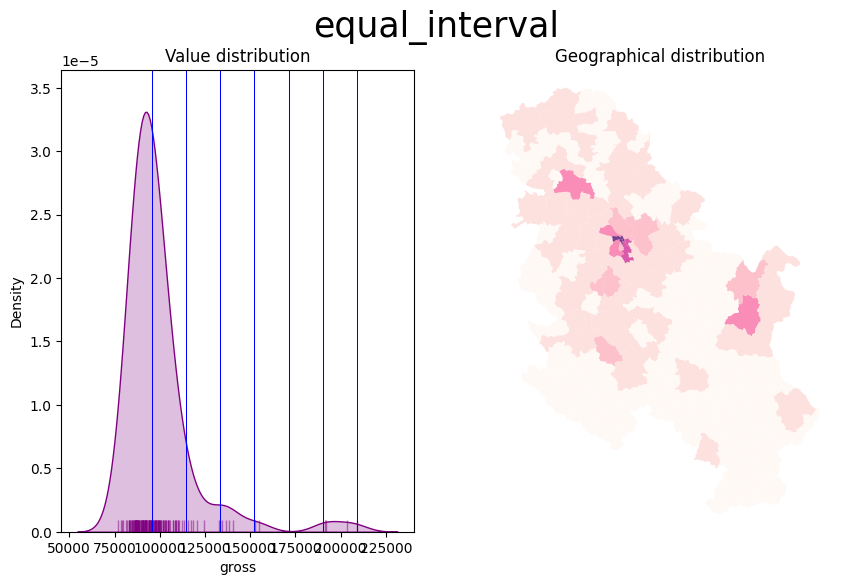
\includegraphics{labs/w02_maps_files/figure-pdf/cell-35-output-1.png}

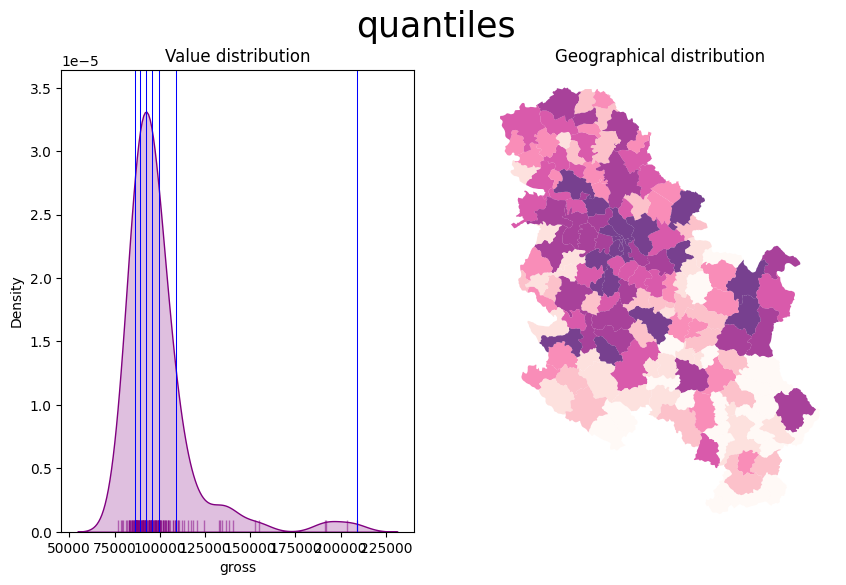
\includegraphics{labs/w02_maps_files/figure-pdf/cell-35-output-2.png}

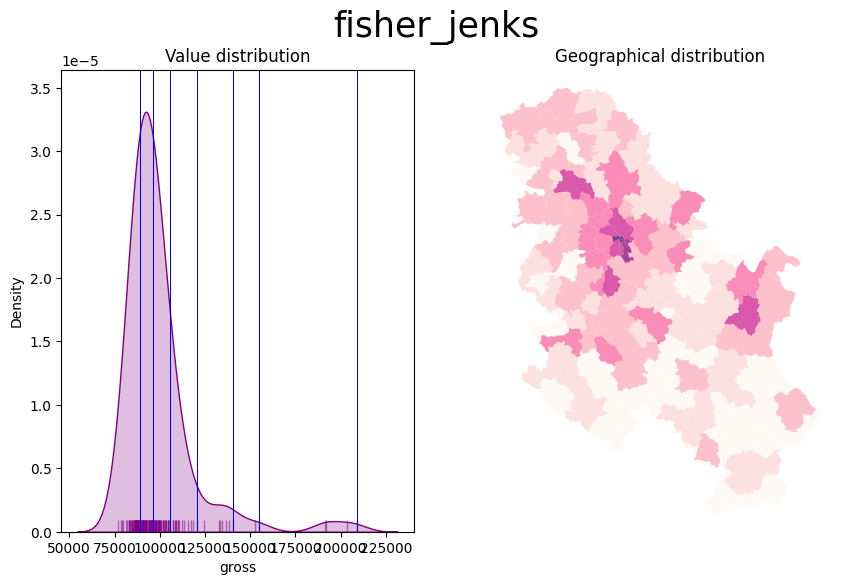
\includegraphics{labs/w02_maps_files/figure-pdf/cell-35-output-3.png}

Also consider the
\href{https://en.wikipedia.org/wiki/Modifiable_areal_unit_problem}{Modifiable
Areal Unit Problem} and how the geographies of the administrative
boundaries, in this case, may impact the visualisation.

For example, the most populated area is a municipality in the north that
corresponds to the city of Novi Sad. Let's have a look at the data

\begin{Shaded}
\begin{Highlighting}[]
\NormalTok{serbia\_admin[[}\StringTok{\textquotesingle{}name\textquotesingle{}}\NormalTok{, }\StringTok{\textquotesingle{}pop\textquotesingle{}}\NormalTok{, }\StringTok{\textquotesingle{}Province\textquotesingle{}}\NormalTok{]].sort\_values(by }\OperatorTok{=} \StringTok{\textquotesingle{}pop\textquotesingle{}}\NormalTok{, ascending }\OperatorTok{=} \VariableTok{False}\NormalTok{).iloc[:}\DecValTok{10}\NormalTok{]}
\end{Highlighting}
\end{Shaded}

\begin{longtable}[]{@{}llll@{}}
\toprule\noalign{}
& name & pop & Province \\
\midrule\noalign{}
\endhead
\bottomrule\noalign{}
\endlastfoot
48 & Novi Sad & 341625.0 & Južno-Bački \\
24 & Novi Beograd & 186667.0 & Grad Beograd \\
19 & Čukarica & 154854.0 & Grad Beograd \\
3 & Kragujevac & 154290.0 & Šumadijski \\
26 & Palilula & 148292.0 & Grad Beograd \\
34 & Zemun & 143173.0 & Grad Beograd \\
32 & Voždovac & 137315.0 & Grad Beograd \\
35 & Zvezdara & 130225.0 & Grad Beograd \\
39 & Leskovac & 123201.0 & Jablanički \\
120 & Subotica & 121250.0 & Severno-Bački \\
\end{longtable}

In our dataset, the city of Novi Sad is categorised as a municipality by
itself, because the administrative boundaries file is not updated. In
reality, ``since 2002, when the new statute of the city of Novi Sad came
into effect, Novi Sad is divided into two city municipalities,
Petrovaradin and Novi Sad. From 1989 until 2002, the name Municipality
of Novi Sad meant the whole territory of the present-day city of Novi
Sad.'' (see:
\href{https://en.wikipedia.org/wiki/City_municipality_of_Novi_Sad}{wikipedia}).

On the contrary, Grad Beograd, that is Belgrade, is correctly split into
different municipalities and its popoulation, when visualised, is spread
out across the different geometries of its municipalities, In other
words, our map depends on the geometries of the areas and on how the
data was collected. While it could be that these areas were indeed
identified by population size in the first place, the point is that the
fact that Novi Sad is not split into more areas, as Belgrade is, makes
it stound out more clearly from the map (and to some extent a bit
unfairly)

This may happen with different types of data, particularly with
administrative boundaries and it is crucial to reflect on how Choropleth
maps may be impacted. One can look for more granular data or consider to
weight the continous value with the texent of the are (i.e.~obtaining
density values).

\subsubsection{An alternative to scheme: ColorMap
Normalisation}\label{an-alternative-to-scheme-colormap-normalisation}

The \texttt{mpl.colors.Normalize} function in \texttt{matplotlib}
creates a normalization object, which adjusts data values into a range
that is ideal for colour mapping in a colormap. This function is
particularly beneficial in scenarios where precise control over the
mapping of data values to colour representations is needed.

When employed in a plotting function, this normalization object ensures
that the data values are scaled to fit a pre-defined range (for
instance, \texttt{norm\ =\ mpl.colors.Normalize(vmin=0,\ vmax=40)}). Any
values falling below 0 are mapped to the lowest colour on the colormap
scale, while values exceeding 40 are mapped to the highest colour. This
approach is especially useful when aiming to highlight differences
within a specific data range; it can significantly enhance the
visualization of data, by, for example, emphasizing temperature
variations between 0°C and 40°C. This becomes crucial in instances where
a few data points with high values (e.g., 50°C) might otherwise lead to
a less informative visualization if not `normalized' and treated as if
they corresponded to 40° C values.

For our dataset, we can use as \texttt{vmax} the value corresponding to
the 90th percentle.

\begin{Shaded}
\begin{Highlighting}[]
\NormalTok{serbia\_admin[}\StringTok{\textquotesingle{}pop\textquotesingle{}}\NormalTok{].quantile(}\FloatTok{0.90}\NormalTok{)}
\end{Highlighting}
\end{Shaded}

\begin{verbatim}
93014.0
\end{verbatim}

\begin{Shaded}
\begin{Highlighting}[]
\ImportTok{import}\NormalTok{ matplotlib }\ImportTok{as}\NormalTok{ mpl}
\NormalTok{fig, ax }\OperatorTok{=}\NormalTok{ plt.subplots(}\DecValTok{1}\NormalTok{, }\DecValTok{1}\NormalTok{)}
\NormalTok{vmin }\OperatorTok{=}\NormalTok{ serbia\_admin[}\StringTok{\textquotesingle{}pop\textquotesingle{}}\NormalTok{].}\BuiltInTok{min}\NormalTok{()}
\NormalTok{vmax }\OperatorTok{=}\NormalTok{ serbia\_admin[}\StringTok{\textquotesingle{}pop\textquotesingle{}}\NormalTok{].quantile(}\FloatTok{0.90}\NormalTok{) }\CommentTok{\# }
\NormalTok{norm }\OperatorTok{=}\NormalTok{ mpl.colors.Normalize(vmin}\OperatorTok{=}\NormalTok{vmin, vmax}\OperatorTok{=}\NormalTok{vmax)}
\NormalTok{serbia\_admin.plot(ax }\OperatorTok{=}\NormalTok{ ax, column}\OperatorTok{=}\StringTok{\textquotesingle{}pop\textquotesingle{}}\NormalTok{, cmap}\OperatorTok{=}\StringTok{\textquotesingle{}OrRd\textquotesingle{}}\NormalTok{, legend}\OperatorTok{=}\VariableTok{True}\NormalTok{, norm }\OperatorTok{=}\NormalTok{ norm)}
\end{Highlighting}
\end{Shaded}

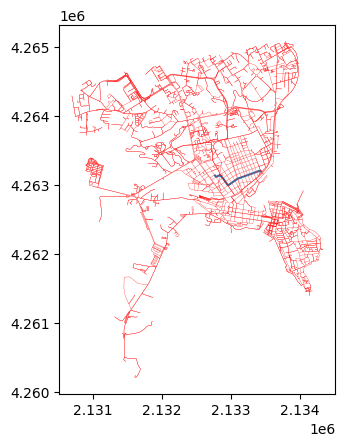
\includegraphics{labs/w02_maps_files/figure-pdf/cell-38-output-1.png}

\textbf{Important}:

When passing \texttt{norm} in the \texttt{plot} method, do not pass the
arguments to the \texttt{scheme} parameter. For continuous variables,
\texttt{norm} maps each value directly to a color, making discrete
categorization redundant. In other words, it allows for a direct mapping
of data values to the color map, eliminating the need for intermediary
classification schemes.\texttt{norm} ensures a smooth gradient in the
color map without artificially segmenting the data.

\subsubsection{Customising the colorbar}\label{customising-the-colorbar}

\begin{Shaded}
\begin{Highlighting}[]
\ImportTok{import}\NormalTok{ matplotlib.cm }\ImportTok{as}\NormalTok{ cm}

\NormalTok{fig, ax }\OperatorTok{=}\NormalTok{ plt.subplots(}\DecValTok{1}\NormalTok{, }\DecValTok{1}\NormalTok{)}
\NormalTok{cmap }\OperatorTok{=} \StringTok{\textquotesingle{}YlOrRd\textquotesingle{}}
\CommentTok{\# we leave the legend out}
\NormalTok{serbia\_admin.plot(column}\OperatorTok{=}\StringTok{\textquotesingle{}pop\textquotesingle{}}\NormalTok{, cmap}\OperatorTok{=}\NormalTok{cmap, norm }\OperatorTok{=}\NormalTok{ norm, ax}\OperatorTok{=}\NormalTok{ax)}

\CommentTok{\# we add the colorbar separately passing the norm and cmap}
\NormalTok{cbar }\OperatorTok{=}\NormalTok{ fig.colorbar(cm.ScalarMappable(norm}\OperatorTok{=}\NormalTok{norm, cmap}\OperatorTok{=}\NormalTok{cmap), ax }\OperatorTok{=}\NormalTok{ ax)}
\NormalTok{cbar.outline.set\_visible(}\VariableTok{False}\NormalTok{)}

\CommentTok{\# updating ticks VALUES}
\NormalTok{ticks }\OperatorTok{=}\NormalTok{ [norm.vmin, norm.vmax]}
\NormalTok{cbar.set\_ticks(ticks }\OperatorTok{=}\NormalTok{ ticks)}

\CommentTok{\# updating ticks LABELS}
\NormalTok{cbar.ax.set\_yticklabels([}\BuiltInTok{round}\NormalTok{(t,}\DecValTok{1}\NormalTok{) }\ControlFlowTok{for}\NormalTok{ t }\KeywordTok{in}\NormalTok{ ticks])}
\NormalTok{cbar.ax.set\_yticklabels([}\BuiltInTok{round}\NormalTok{(t,}\DecValTok{1}\NormalTok{) }\ControlFlowTok{if}\NormalTok{ t }\OperatorTok{\textless{}}\NormalTok{ norm.vmax }\ControlFlowTok{else} \StringTok{"\textgreater{}= "}\OperatorTok{+}\BuiltInTok{str}\NormalTok{(}\BuiltInTok{round}\NormalTok{(t,}\DecValTok{1}\NormalTok{)) }\ControlFlowTok{for}\NormalTok{ t }\KeywordTok{in}\NormalTok{ cbar.ax.get\_yticks()])}
\end{Highlighting}
\end{Shaded}

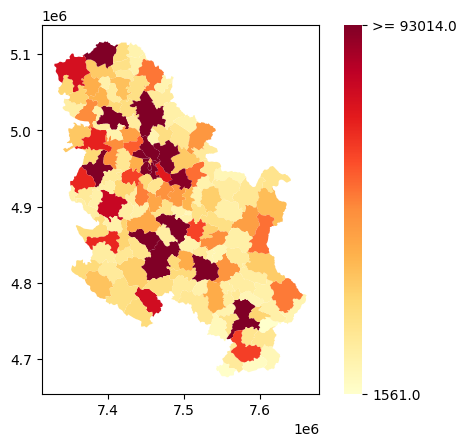
\includegraphics{labs/w02_maps_files/figure-pdf/cell-39-output-1.png}

Above, we removed the outline of the color bar. Then we set the tick
values to the min and the max population values, based on our norm
object. Then, for the vmax value's label we added a ``\textgreater='' to
remind us that other, higher values are displayed with the darkest
color.

\subsubsection{Varying alpha transparency based on an
array}\label{varying-alpha-transparency-based-on-an-array}

Finally, we can also convey variation in a continuos scale through
transparency. \texttt{alpha} doesn't expect column names, so we cannot
just pass the name of the column containing the variable. Instead we
have to create an array from 0.0 to 1.0 values. To so we can a) use
normalisation methods, or b) rescale the original values within 0 to 1
based on the original min and max values.

For example, with square root normalization:

\begin{Shaded}
\begin{Highlighting}[]
\CommentTok{\# 1. Create an alpha array based on a normalized value (e.g., population)}
\ImportTok{import}\NormalTok{ numpy }\ImportTok{as}\NormalTok{ np}
\NormalTok{pop\_max }\OperatorTok{=}\NormalTok{ serbia\_admin[}\StringTok{\textquotesingle{}pop\textquotesingle{}}\NormalTok{].}\BuiltInTok{max}\NormalTok{()}
\NormalTok{alpha }\OperatorTok{=}\NormalTok{ np.sqrt(serbia\_admin[}\StringTok{\textquotesingle{}pop\textquotesingle{}}\NormalTok{] }\OperatorTok{/}\NormalTok{ pop\_max) }
\end{Highlighting}
\end{Shaded}

\begin{Shaded}
\begin{Highlighting}[]
\CommentTok{\# Plot with varying alpha values}
\NormalTok{fig, axes }\OperatorTok{=}\NormalTok{ plt.subplots(}\DecValTok{1}\NormalTok{, }\DecValTok{2}\NormalTok{, figsize}\OperatorTok{=}\NormalTok{(}\DecValTok{10}\NormalTok{, }\DecValTok{6}\NormalTok{))}
\NormalTok{serbia\_admin.plot(color }\OperatorTok{=} \StringTok{\textquotesingle{}blue\textquotesingle{}}\NormalTok{, ax}\OperatorTok{=}\NormalTok{axes[}\DecValTok{0}\NormalTok{], alpha}\OperatorTok{=}\NormalTok{alpha, edgecolor}\OperatorTok{=}\StringTok{\textquotesingle{}black\textquotesingle{}}\NormalTok{, linewidth }\OperatorTok{=} \FloatTok{0.3}\NormalTok{) }\CommentTok{\#one color}
\NormalTok{serbia\_admin.plot(cmap }\OperatorTok{=} \StringTok{\textquotesingle{}YlOrRd\textquotesingle{}}\NormalTok{, ax}\OperatorTok{=}\NormalTok{axes[}\DecValTok{1}\NormalTok{], alpha}\OperatorTok{=}\NormalTok{alpha, edgecolor}\OperatorTok{=}\StringTok{\textquotesingle{}red\textquotesingle{}}\NormalTok{, linewidth }\OperatorTok{=} \FloatTok{0.3}\NormalTok{) }\CommentTok{\#cmap}
\ControlFlowTok{for}\NormalTok{ ax }\KeywordTok{in}\NormalTok{ axes:}
\NormalTok{    ax.set\_axis\_off()}
\end{Highlighting}
\end{Shaded}

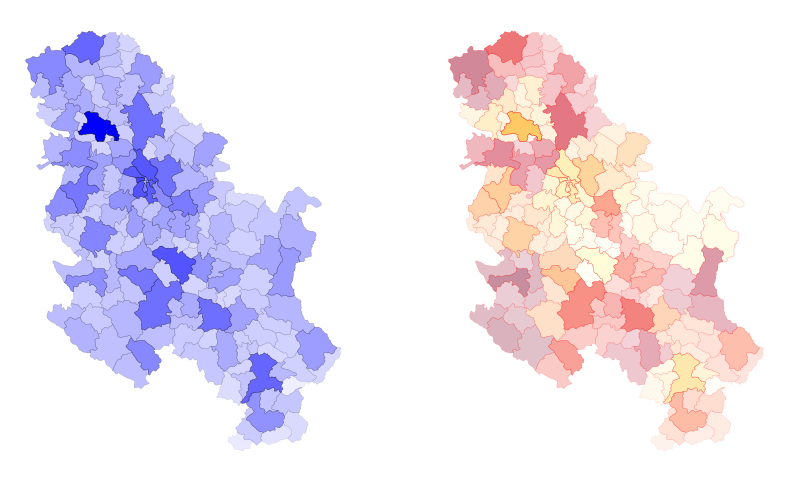
\includegraphics{labs/w02_maps_files/figure-pdf/cell-41-output-1.png}

\textbf{Important}:

\texttt{matplotlib} would not able to plot a color bar from variations
in the alpha value since no column is passed directly. We would need, in
this case, to build a color bar manually as demonstrated above.

\subsection{Choropleth Maps for Categorical
Variables}\label{choropleth-maps-for-categorical-variables}

A choropleth for categorical variables assigns a different color to
every potential value in the series based on certain colormaps
(\texttt{cmap}). We don't need to specify a scheme in this case, but
just to the categorical \texttt{column}. Using last's week GeoDataFrame,
we can plot terrorist attacks in Germany, for example, by group.

\begin{Shaded}
\begin{Highlighting}[]
\NormalTok{gdf }\OperatorTok{=}\NormalTok{ gpd.read\_file(}\StringTok{"../data/germany.shp"}\NormalTok{).to\_crs(germany\_crs)}
\NormalTok{fig, ax }\OperatorTok{=}\NormalTok{ plt.subplots(}\DecValTok{1}\NormalTok{, }\DecValTok{1}\NormalTok{, figsize}\OperatorTok{=}\NormalTok{(}\DecValTok{8}\NormalTok{, }\DecValTok{6}\NormalTok{))}
\NormalTok{gdf.plot(ax }\OperatorTok{=}\NormalTok{ ax, column }\OperatorTok{=} \StringTok{\textquotesingle{}gname\textquotesingle{}}\NormalTok{, legend }\OperatorTok{=} \VariableTok{True}\NormalTok{)}
\NormalTok{ax.set\_axis\_off()}
\NormalTok{title\_parameters }\OperatorTok{=}\NormalTok{ \{}\StringTok{\textquotesingle{}fontsize\textquotesingle{}}\NormalTok{:}\StringTok{\textquotesingle{}16\textquotesingle{}}\NormalTok{, }\StringTok{\textquotesingle{}fontname\textquotesingle{}}\NormalTok{:}\StringTok{\textquotesingle{}Times New Roman\textquotesingle{}}\NormalTok{\}}
\NormalTok{ax.set\_title(}\StringTok{"Terrorist Attacks in Germany, by Group"}\NormalTok{, }\OperatorTok{**}\NormalTok{title\_parameters) }\CommentTok{\#parameters as above}
\end{Highlighting}
\end{Shaded}

\begin{verbatim}
Text(0.5, 1.0, 'Terrorist Attacks in Germany, by Group')
\end{verbatim}

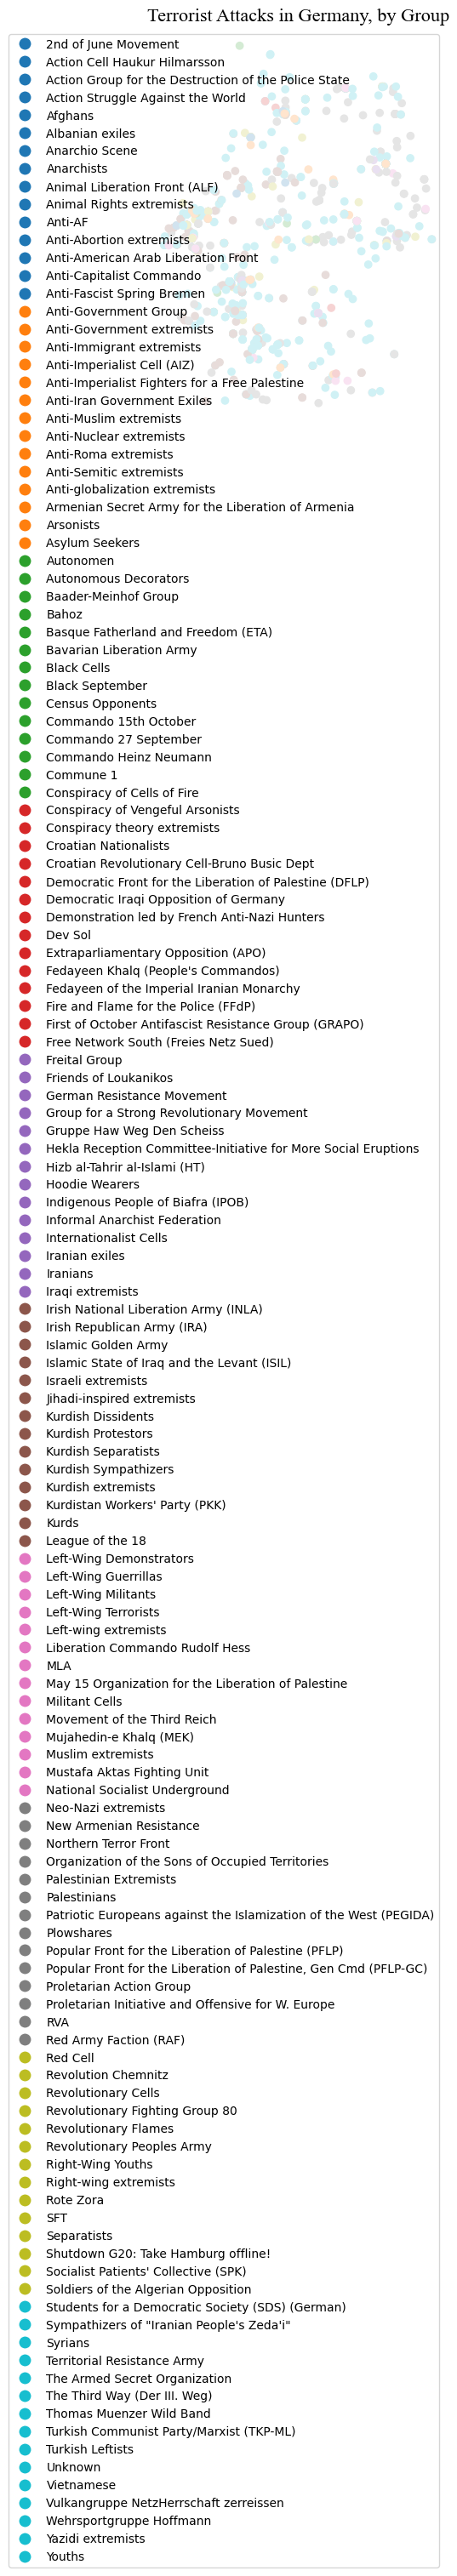
\includegraphics{labs/w02_maps_files/figure-pdf/cell-42-output-2.png}

The map above is what you would get from datasets that are not
cleaned/manipulated directly or when there are too many categories in
the selected column. First, let's get a slimmer slice of the gdf that
only contains attacks that cause a number of fatalies and wounded higher
than 10.

\begin{Shaded}
\begin{Highlighting}[]
\NormalTok{condition }\OperatorTok{=}\NormalTok{ (gdf.nkill }\OperatorTok{+}\NormalTok{ gdf.nwound) }\OperatorTok{\textgreater{}} \DecValTok{10}
\NormalTok{gdf\_filtered }\OperatorTok{=}\NormalTok{ gdf[condition].copy()}
\end{Highlighting}
\end{Shaded}

Then, let's build a function that creates a random color map based on
the number of categories. This creates random \texttt{HUE}-based colors:

\begin{Shaded}
\begin{Highlighting}[]
\CommentTok{\# Generate random colormap}
\KeywordTok{def}\NormalTok{ rand\_cmap(nlabels):}
    \CommentTok{""" }
\CommentTok{    It generates a categorical random color map, given the number of classes}
\CommentTok{    }
\CommentTok{    Parameters}
\CommentTok{    {-}{-}{-}{-}{-}{-}{-}{-}{-}{-}}
\CommentTok{    nlabels: int}
\CommentTok{        The number of categories to be coloured.}
\CommentTok{    type\_color: str \{"soft", "bright"\} }
\CommentTok{        It defines whether using bright or soft pastel colors, by limiting the RGB spectrum.}
\CommentTok{       }
\CommentTok{    Returns}
\CommentTok{    {-}{-}{-}{-}{-}{-}{-}}
\CommentTok{    cmap: matplotlib.colors.LinearSegmentedColormap}
\CommentTok{        The color map.}
\CommentTok{    """}   
    \CommentTok{\# Generate color map for bright colors, based on hsv}
\NormalTok{    randHSVcolors }\OperatorTok{=}\NormalTok{ [(np.random.uniform(low}\OperatorTok{=}\FloatTok{0.20}\NormalTok{, high}\OperatorTok{=}\FloatTok{0.80}\NormalTok{),}
\NormalTok{                          np.random.uniform(low}\OperatorTok{=}\FloatTok{0.20}\NormalTok{, high}\OperatorTok{=}\FloatTok{0.80}\NormalTok{),}
\NormalTok{                          np.random.uniform(low}\OperatorTok{=}\FloatTok{0.20}\NormalTok{, high}\OperatorTok{=} \FloatTok{0.80}\NormalTok{)) }\ControlFlowTok{for}\NormalTok{ i }\KeywordTok{in} \BuiltInTok{range}\NormalTok{(nlabels)]}

\NormalTok{    random\_colormap }\OperatorTok{=}\NormalTok{ LinearSegmentedColormap.from\_list(}\StringTok{\textquotesingle{}new\_map\textquotesingle{}}\NormalTok{, randHSVcolors, N}\OperatorTok{=}\NormalTok{nlabels)}
   
    \ControlFlowTok{return}\NormalTok{ random\_colormap }
\end{Highlighting}
\end{Shaded}

\begin{Shaded}
\begin{Highlighting}[]
\NormalTok{cmap }\OperatorTok{=}\NormalTok{ rand\_cmap(}\BuiltInTok{len}\NormalTok{(gdf\_filtered.gname.unique()))}
\NormalTok{cmap}
\end{Highlighting}
\end{Shaded}


\includegraphics{labs/w02_maps_files/figure-pdf/cell-45-output-1.png}

We also place the legend on the center left. This is done automatically,
but the legend and its items can be manipulated directly. Legends in
\texttt{matplotlib} are extremely complex to personalise. However, do
have a look at
https://matplotlib.org/stable/api/\_as\_gen/matplotlib.pyplot.legend.html\#matplotlib.pyplot.legend
for both automatic and explicit manipulation.

\begin{Shaded}
\begin{Highlighting}[]
\NormalTok{legend\_kwds}\OperatorTok{=}\NormalTok{\{}\StringTok{"loc"}\NormalTok{: }\StringTok{"center left"}\NormalTok{, }\StringTok{"bbox\_to\_anchor"}\NormalTok{: (}\DecValTok{1}\NormalTok{, }\FloatTok{0.5}\NormalTok{)\}}
\end{Highlighting}
\end{Shaded}

\begin{Shaded}
\begin{Highlighting}[]
\NormalTok{fig, ax }\OperatorTok{=}\NormalTok{ plt.subplots(}\DecValTok{1}\NormalTok{, }\DecValTok{1}\NormalTok{, figsize}\OperatorTok{=}\NormalTok{(}\DecValTok{8}\NormalTok{, }\DecValTok{6}\NormalTok{))}
\NormalTok{gdf\_filtered.plot(ax }\OperatorTok{=}\NormalTok{ ax, column }\OperatorTok{=} \StringTok{\textquotesingle{}gname\textquotesingle{}}\NormalTok{, legend }\OperatorTok{=} \VariableTok{True}\NormalTok{, cmap }\OperatorTok{=}\NormalTok{ cmap, legend\_kwds }\OperatorTok{=}\NormalTok{ legend\_kwds)}
\NormalTok{title\_parameters }\OperatorTok{=}\NormalTok{ \{}\StringTok{\textquotesingle{}fontsize\textquotesingle{}}\NormalTok{:}\StringTok{\textquotesingle{}16\textquotesingle{}}\NormalTok{, }\StringTok{\textquotesingle{}fontname\textquotesingle{}}\NormalTok{:}\StringTok{\textquotesingle{}Times New Roman\textquotesingle{}}\NormalTok{\}}
\NormalTok{ax.set\_title(}\StringTok{"Terrorist Attacks in Germany, by Group"}\NormalTok{, }\OperatorTok{**}\NormalTok{title\_parameters) }\CommentTok{\#parameters as above}
\NormalTok{ctx.add\_basemap(ax, crs}\OperatorTok{=}\NormalTok{ gdf\_filtered.crs.to\_string(), source }\OperatorTok{=}\NormalTok{ ctx.providers.Esri.WorldGrayCanvas)}
\end{Highlighting}
\end{Shaded}

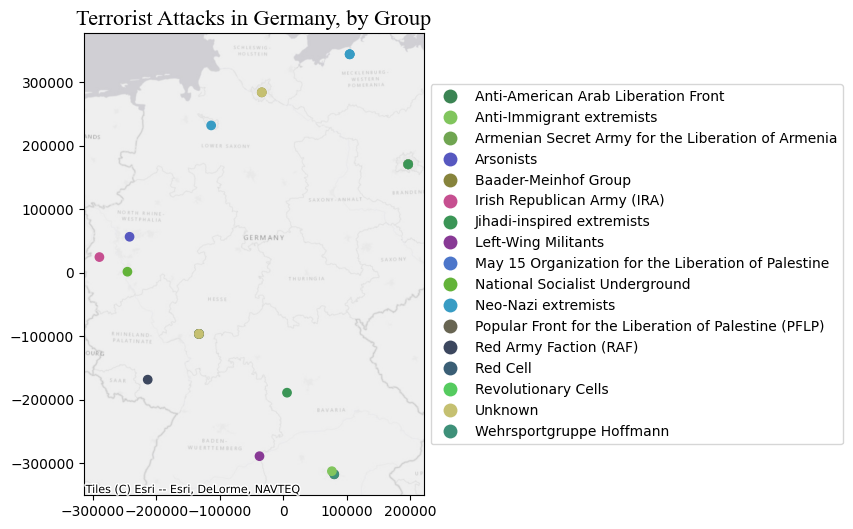
\includegraphics{labs/w02_maps_files/figure-pdf/cell-47-output-1.png}

We can also convey the impact of the events through the
\texttt{markersize}. This introduces the concept of \emph{cartogram}
(see below).

\begin{Shaded}
\begin{Highlighting}[]
\NormalTok{fig, ax }\OperatorTok{=}\NormalTok{ plt.subplots(}\DecValTok{1}\NormalTok{, }\DecValTok{1}\NormalTok{, figsize}\OperatorTok{=}\NormalTok{(}\DecValTok{8}\NormalTok{, }\DecValTok{6}\NormalTok{))}
\NormalTok{gdf\_filtered.plot(ax }\OperatorTok{=}\NormalTok{ ax, column }\OperatorTok{=} \StringTok{\textquotesingle{}gname\textquotesingle{}}\NormalTok{, markersize }\OperatorTok{=} \StringTok{\textquotesingle{}nwound\textquotesingle{}}\NormalTok{, legend }\OperatorTok{=} \VariableTok{True}\NormalTok{, cmap }\OperatorTok{=}\NormalTok{ cmap, legend\_kwds }\OperatorTok{=}\NormalTok{ legend\_kwds)}
\NormalTok{ax.set\_title(}\StringTok{"Terrorist Attacks in Germany, by Group"}\NormalTok{, }\OperatorTok{**}\NormalTok{title\_parameters) }\CommentTok{\#parameters as above}
\NormalTok{ctx.add\_basemap(ax, crs}\OperatorTok{=}\NormalTok{ gdf\_filtered.crs.to\_string(), source }\OperatorTok{=}\NormalTok{ ctx.providers.Esri.WorldGrayCanvas)}
\NormalTok{ax.set\_axis\_off()}
\end{Highlighting}
\end{Shaded}

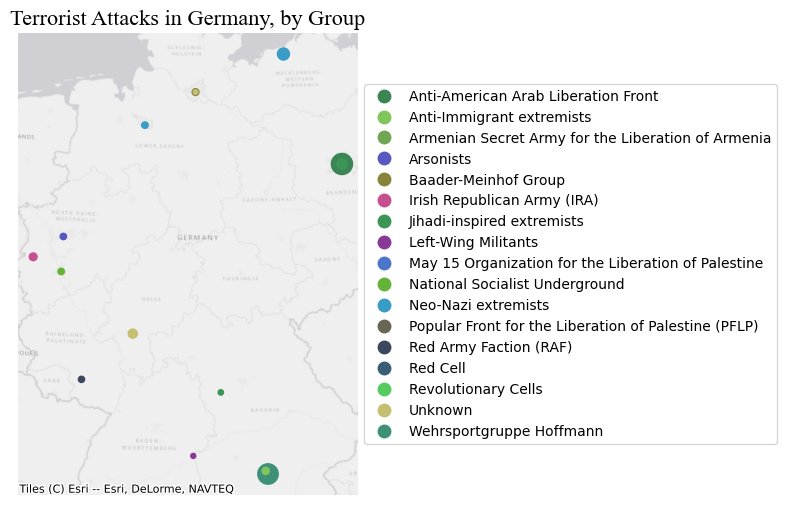
\includegraphics{labs/w02_maps_files/figure-pdf/cell-48-output-1.png}

\section{Part III: Cartograms - Manipulating the Geometry size for
showing the magitude of a
value}\label{part-iii-cartograms---manipulating-the-geometry-size-for-showing-the-magitude-of-a-value}

\href{https://www.data-to-viz.com/graph/cartogram.html}{Cartograms} are
maps that represent the spatial distribution of a variable not by
encoding it in a color palette but rather by modifying geographical
objects. There are many algorithms to distort the shapes of geographical
entities according to values, some of them incredibly complicated and
complex.

\subsection{Polygons}\label{polygons}

You can obtain cartograms for \texttt{Polygon} with \texttt{geoplot}:
see https://residentmario.github.io/geoplot/

\texttt{geoplot} functions pretty much work as \texttt{plot}

\begin{Shaded}
\begin{Highlighting}[]
\CommentTok{\# this library needs the GeoDataFrame to be reverted to WGS}
\NormalTok{ax }\OperatorTok{=}\NormalTok{ gplt.cartogram(serbia\_admin.to\_crs(wgs), scale}\OperatorTok{=}\StringTok{\textquotesingle{}pop\textquotesingle{}}\NormalTok{, projection}\OperatorTok{=}\NormalTok{gcrs.Mercator(), color }\OperatorTok{=} \StringTok{\textquotesingle{}darkblue\textquotesingle{}}\NormalTok{)}
\CommentTok{\# see for projections that work with gplt https://scitools.org.uk/cartopy/docs/v0.15/crs/projections.html}
\NormalTok{gplt.polyplot(serbia\_admin.to\_crs(wgs), facecolor}\OperatorTok{=}\StringTok{\textquotesingle{}lightgray\textquotesingle{}}\NormalTok{, edgecolor}\OperatorTok{=}\StringTok{\textquotesingle{}white\textquotesingle{}}\NormalTok{, ax}\OperatorTok{=}\NormalTok{ax, lw }\OperatorTok{=} \FloatTok{0.5}\NormalTok{) }\CommentTok{\# this is just for comparison}
\end{Highlighting}
\end{Shaded}

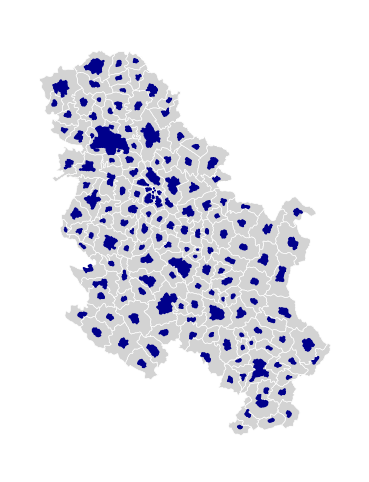
\includegraphics{labs/w02_maps_files/figure-pdf/cell-49-output-1.png}

\subsection{Points}\label{points}

For \texttt{Point} GeoDataFrames we can just go back to \texttt{plot}
and pass a column name to \texttt{markersize}.

\begin{Shaded}
\begin{Highlighting}[]
\NormalTok{attacks }\OperatorTok{=}\NormalTok{ pd.read\_csv(}\StringTok{"../data/GTD\_2022.csv"}\NormalTok{, low\_memory }\OperatorTok{=} \VariableTok{False}\NormalTok{)}
\NormalTok{country }\OperatorTok{=} \StringTok{\textquotesingle{}Germany\textquotesingle{}}

\NormalTok{df }\OperatorTok{=}\NormalTok{ attacks[attacks.country\_txt }\OperatorTok{==}\NormalTok{ country].copy()}
\NormalTok{wgs }\OperatorTok{=} \StringTok{\textquotesingle{}EPSG:4326\textquotesingle{}}
\NormalTok{germany\_crs }\OperatorTok{=} \StringTok{\textquotesingle{}EPSG:4839\textquotesingle{}}
\NormalTok{gdf }\OperatorTok{=}\NormalTok{ gpd.GeoDataFrame(df, geometry}\OperatorTok{=}\NormalTok{gpd.points\_from\_xy(df.longitude, df.latitude), crs }\OperatorTok{=}\NormalTok{ wgs)}
\NormalTok{gdf }\OperatorTok{=}\NormalTok{ gdf.to\_crs(germany\_crs)}
\end{Highlighting}
\end{Shaded}

\begin{Shaded}
\begin{Highlighting}[]
\NormalTok{fig, ax }\OperatorTok{=}\NormalTok{ plt.subplots(}\DecValTok{1}\NormalTok{, }\DecValTok{1}\NormalTok{, figsize}\OperatorTok{=}\NormalTok{(}\DecValTok{8}\NormalTok{, }\DecValTok{6}\NormalTok{))}
\NormalTok{gdf.plot(ax }\OperatorTok{=}\NormalTok{ ax, markersize }\OperatorTok{=} \StringTok{\textquotesingle{}nwound\textquotesingle{}}\NormalTok{, color }\OperatorTok{=} \StringTok{\textquotesingle{}purple\textquotesingle{}}\NormalTok{, legend }\OperatorTok{=} \VariableTok{True}\NormalTok{)}
\NormalTok{ax.set\_axis\_off()}
\end{Highlighting}
\end{Shaded}


\includegraphics{labs/w02_maps_files/figure-pdf/cell-51-output-1.png}

One can also convert convert polygons into points by using their
centroids, and then define the size of the dot proportionally to the
value of the variable we want to display.

\subsection{LineString}\label{linestring}

For \texttt{LineString} we pass the column name to \texttt{linewidth}.

Let's load a shapefile of lines. These lines represent frequnecy of
train connections from/to train stations in the region of Liguria
(Italy) to other stations within or outside the region. Each line refers
to a connection between two specific stations, through a certain type of
service and contains information about the frequency of that type of
service. For example, the cities of Savona and Finale Ligure might be
connected by 5 InterCity trains and 50 regional services. These services
correspond to 2 different records.

\begin{Shaded}
\begin{Highlighting}[]
\NormalTok{trains\_freq }\OperatorTok{=}\NormalTok{ gpd.read\_file(}\StringTok{"../data/trains\_liguria.shp"}\NormalTok{ )}
\NormalTok{trains\_freq.crs}
\end{Highlighting}
\end{Shaded}

\begin{verbatim}
<Projected CRS: EPSG:3003>
Name: Monte Mario / Italy zone 1
Axis Info [cartesian]:
- X[east]: Easting (metre)
- Y[north]: Northing (metre)
Area of Use:
- name: Italy - onshore and offshore - west of 12°E.
- bounds: (5.93, 36.53, 12.0, 47.04)
Coordinate Operation:
- name: Italy zone 1
- method: Transverse Mercator
Datum: Monte Mario
- Ellipsoid: International 1924
- Prime Meridian: Greenwich
\end{verbatim}

Let's check the type of services contained here.

\begin{Shaded}
\begin{Highlighting}[]
\NormalTok{trains\_freq[}\StringTok{\textquotesingle{}train\_type\textquotesingle{}}\NormalTok{].unique()}
\end{Highlighting}
\end{Shaded}

\begin{verbatim}
array(['REG', 'IC', 'FB', 'ICN', 'U', 'EC/EN', 'AV'], dtype=object)
\end{verbatim}

We have: - `REG': regional trains. - `IC': intercity trains. - `FB':
similar to IC, but slightly faster. - `ICN': sleeper trains. - `U':
urban trains (Genoa). - `EC/EN': international trains. - `AV':
High-speed trains.

Let's keep just regional, intercity, and high-speed trains.

\begin{Shaded}
\begin{Highlighting}[]
\NormalTok{to\_keep }\OperatorTok{=}\NormalTok{ [}\StringTok{\textquotesingle{}REG\textquotesingle{}}\NormalTok{, }\StringTok{\textquotesingle{}IC\textquotesingle{}}\NormalTok{, }\StringTok{\textquotesingle{}AV\textquotesingle{}}\NormalTok{]}
\NormalTok{trains\_freq }\OperatorTok{=}\NormalTok{ trains\_freq[trains\_freq[}\StringTok{\textquotesingle{}train\_type\textquotesingle{}}\NormalTok{].isin(to\_keep)]}
\end{Highlighting}
\end{Shaded}

The usage of \texttt{linewdith} is a bit different from
\texttt{markersize} for some reason. We have to pass an \texttt{array}
of N values, where N is equal to the GeoDataFrame size. In other words,
we have to pass the column we want to use to regulate the line width
direclty as a list/array. Specifying the column name is not enough.

\begin{Shaded}
\begin{Highlighting}[]
\NormalTok{fig, ax }\OperatorTok{=}\NormalTok{ plt.subplots(}\DecValTok{1}\NormalTok{, }\DecValTok{1}\NormalTok{, figsize}\OperatorTok{=}\NormalTok{(}\DecValTok{10}\NormalTok{, }\DecValTok{15}\NormalTok{))}
\NormalTok{trains\_freq.plot(ax }\OperatorTok{=}\NormalTok{ ax, linewidth }\OperatorTok{=}\NormalTok{ trains\_freq[}\StringTok{\textquotesingle{}freq\textquotesingle{}}\NormalTok{])}
\NormalTok{ax.set\_axis\_off()}
\end{Highlighting}
\end{Shaded}

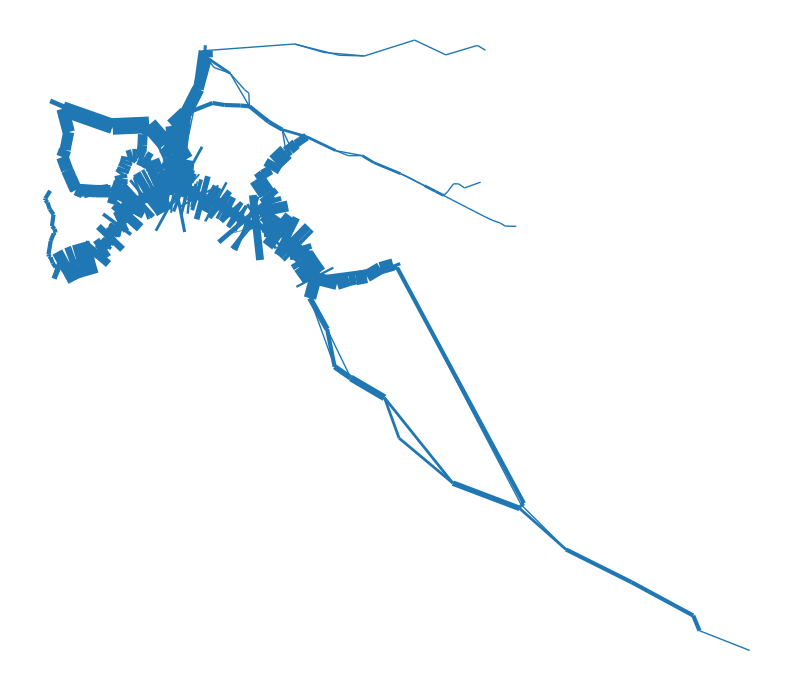
\includegraphics{labs/w02_maps_files/figure-pdf/cell-55-output-1.png}

As you can see, the default arguments and simply passing the column
values do not produce pretty results. The first thing to look at is the
values that are passed to \texttt{linewidth}. In some cases the min and
max values, as well as their distribution, are not ideal for visually
conveying the magnitude of the variable attached to the geometry. One
option is to use a multiplier factor (see below), or to rescale the
values from 0 to 1, for example, and then, again, if necessary use a
multiplier.

\begin{Shaded}
\begin{Highlighting}[]
\NormalTok{fig, ax }\OperatorTok{=}\NormalTok{ plt.subplots(}\DecValTok{1}\NormalTok{, }\DecValTok{1}\NormalTok{, figsize}\OperatorTok{=}\NormalTok{(}\DecValTok{15}\NormalTok{, }\DecValTok{20}\NormalTok{))}
\NormalTok{lw }\OperatorTok{=}\NormalTok{ trains\_freq[}\StringTok{\textquotesingle{}freq\textquotesingle{}}\NormalTok{] }\OperatorTok{*} \FloatTok{0.15}
\NormalTok{trains\_freq.plot(ax }\OperatorTok{=}\NormalTok{ ax, linewidth }\OperatorTok{=}\NormalTok{ lw, capstyle }\OperatorTok{=} \StringTok{\textquotesingle{}round\textquotesingle{}}\NormalTok{, joinstyle }\OperatorTok{=} \StringTok{\textquotesingle{}round\textquotesingle{}}\NormalTok{, column }\OperatorTok{=} \StringTok{\textquotesingle{}train\_type\textquotesingle{}}\NormalTok{, legend }\OperatorTok{=} \VariableTok{True}\NormalTok{)}
\NormalTok{ctx.add\_basemap(ax, crs}\OperatorTok{=}\NormalTok{ trains\_freq.crs.to\_string(), source }\OperatorTok{=}\NormalTok{ ctx.providers.Esri.WorldGrayCanvas)}
\NormalTok{ax.set\_axis\_off()}
\end{Highlighting}
\end{Shaded}

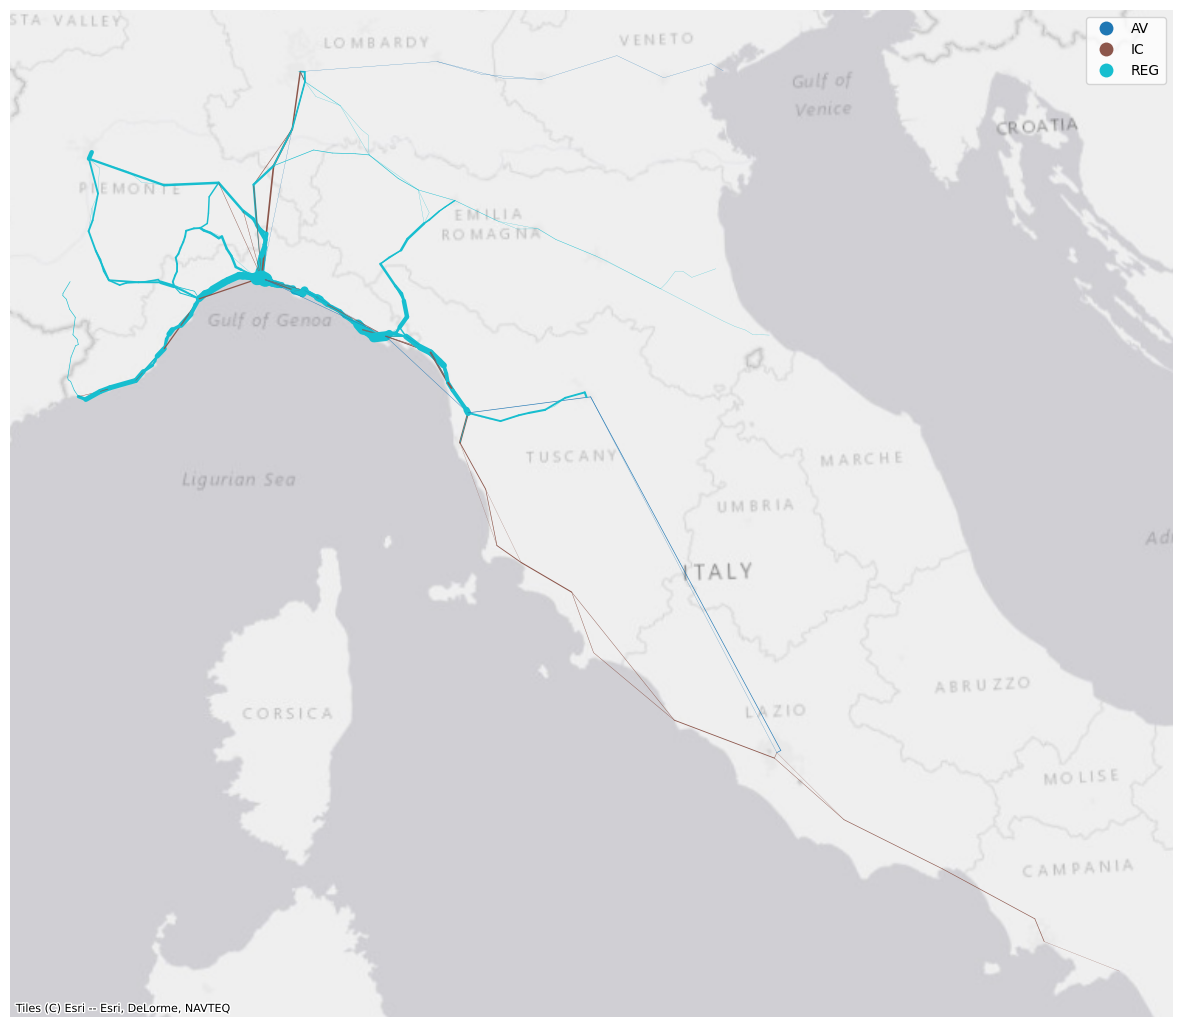
\includegraphics{labs/w02_maps_files/figure-pdf/cell-56-output-1.png}

While this looks a bit better, this visualisation is not ideal because
the frequencies are not snapped to the actual railway network. The lines
represent instead connection between train stops and therefore their
coordinatse only include the ones corresponding to the stations where
the different services call at. One can devise approaches to:

\begin{itemize}
\tightlist
\item
  Assigning the frequencies, or any other value, to the corresponding
  infrastructure's section. For example, the railway section between two
  stations could be associated with a value representing the total
  number of REG services along it.
\item
  Smoothing the lines representing the services by adding further
  coordinates along the line.
\end{itemize}

Both these processes go beyond the scopes of this lab and require
several considerations depending on the data, the scale, and what
information one wants to displays.

\textbf{Exercise}:

Today we've seen how to exploit matplotlib to plot GeoDataFrame. Go
through the notebook again if you feel that there's something you need
to review. You are not expected to remember each step/method/parameter.
Rather, this notebook should be used as a reference from producing maps
in python. Do keep in mind that most of the maps above have been
produced with just a bunch of rows, so each of them can be improved and
embellished with some more effort.

Now, if you are not overwhelmed, have a look at the very last map and
produce some nice visualisation using the same data. You can further
improve it clarity, add a legend that refers to the line width,
visualise only a certain type of service, or add information/context,
for example. In the folder `\data' you can also find a shapefile
containing all the train stations in Italy, should you need that.

\subsubsection{\texorpdfstring{Saving figures (check
\href{https://matplotlib.org/stable/api/_as_gen/matplotlib.pyplot.savefig.html}{here
for
details})}{Saving figures (check here for details)}}\label{saving-figures-check-here-for-details}

\begin{Shaded}
\begin{Highlighting}[]
\NormalTok{fig.savefig(}\StringTok{"fig1.pdf"}\NormalTok{, dpi}\OperatorTok{=}\StringTok{\textquotesingle{}figure\textquotesingle{}}\NormalTok{, }\BuiltInTok{format}\OperatorTok{=}\StringTok{"pdf"}\NormalTok{, bbox\_inches }\OperatorTok{=} \StringTok{\textquotesingle{}tight\textquotesingle{}}\NormalTok{)}
\end{Highlighting}
\end{Shaded}

\bookmarksetup{startatroot}

\chapter{Web Architectures and APIs}\label{web-architectures-and-apis}

The \textbf{Lecture slides} can be found
\href{https://github.com/GDSL-UL/wma/raw/main/lectures/w03.html}{here}.

\section{What do APIs actually do?}\label{what-do-apis-actually-do}

In this lab, we will unpack how Application Programming Interfaces
(``APIs'') work and we cover the basics of accessing an API using
Python. Instead of downloading a data set, APIs allow programmers,
statisticians (or students) to request data directly from a server to a
local machine. When you work with web APIs, two different computers ---
a client and server --- will interact with each other to request and
provide data, respectively.

\subsection{RESTful Web APIs are all around
you.}\label{restful-web-apis-are-all-around-you.}

\textbf{Web APIs}

\begin{itemize}
\tightlist
\item
  Allow you query a remote database over the internet
\item
  Take on a variety of formats
\item
  Adhere to a particular style known as Representation State Transfer or
  REST (in most cases)
\item
  RESTful APIs are convenient because we use them to query database
  using URLs
\end{itemize}

\textbf{Consider a simple Google search:}

Ever wonder what all that extra stuff in the address bar was all about?
In this case, the full address is Google's way of sending a query to its
databases requesting information related to the search term
\emph{liverpool top attractions}.

In fact, it looks like Google makes its query by taking the search
terms, separating each of them with a \textbf{+}, and appending them to
the link \url{https://www.google.com/\#q=}. Therefore, we should be able
to actually change our Google search by adding some terms to the URL:

Learning how to use RESTful APIs is all about learning how to format
these URLs so that you can get the response you want.

\subsection{Group activity}\label{group-activity}

Get into groups of 5 or 6 students. Using your friend the internet, look
up answers to the following questions. Each group will be assigned one
question and asked to present their findings in 5 min to discuss with
the entire class.

\begin{enumerate}
\def\labelenumi{\arabic{enumi}.}
\tightlist
\item
  What is a \texttt{URL} and how can it help us query data? What is a
  response status and what are the possible categories?
\item
  What is a \texttt{GET} request? How does a \texttt{GET} request work?
\item
  What are API keys and how do you obtain them? What kinds of
  restrictions to they impose on users? Find an example of an API key,
  what does it look like?
\item
  (For 2 groups) More and more APIs pop up every day. Do a bit of quick
  research and find 2 different examples of APIs that you would be
  interested in using. 2 groups, 2 or 3 APIs each.
\end{enumerate}

There are two ways to collect data through APIs in Python:

\begin{itemize}
\tightlist
\item
  \textbf{Plug-n-play packages.} Many common APIs are available through
  user-written Python (or R) Packages. These packages offer functions
  that conveniently ``wrap'' API queries and format the response. These
  packages are usually much more convenient than writing our own query,
  so it is worth searching for a package that works with the API we
  need.
\item
  \textbf{Writing our own API request.} If no wrapper function is
  available, web have to write our own API request and format the
  response ourselves using Python. This is tricky, but definitely
  doable.
\end{itemize}

\section{API Python libraries}\label{api-python-libraries}

\textbf{Exercise: \texttt{census} pair activity}:

Some Python packages ``wrap'' API queries and format the response. Lucky
us! In pairs, let's have a look at
\href{https://github.com/datamade/census/tree/master}{\texttt{census}},
a wrapper or the United States Census Bureau's API You can also have a
look at the different APIs available from the
\href{https://www.census.gov/data/developers.html}{United States Census
Bureau}.

\begin{Shaded}
\begin{Highlighting}[]
\ImportTok{import}\NormalTok{ pandas }\ImportTok{as}\NormalTok{ pd}
\ImportTok{from}\NormalTok{ census }\ImportTok{import}\NormalTok{ Census}
\end{Highlighting}
\end{Shaded}

To get started working, set you Census API key. A key can be obtained
from http://api.census.gov/data/key\_signup.html.

\begin{Shaded}
\begin{Highlighting}[]
\NormalTok{census\_api\_key }\OperatorTok{=} \StringTok{""} \CommentTok{\# Replace \textquotesingle{}YOUR\_CENSUS\_API\_KEY\_HERE\textquotesingle{} with your actual Census API key.}
\end{Highlighting}
\end{Shaded}

\begin{Shaded}
\begin{Highlighting}[]
\CommentTok{\# Set API key}
\NormalTok{c }\OperatorTok{=}\NormalTok{ Census(census\_api\_key)}
\end{Highlighting}
\end{Shaded}

\begin{itemize}
\tightlist
\item
  Variables in tidycensus are identified by their Census ID,
  e.g.~B19013\_001.
\item
  Entire tables of variables can be requested with the table argument,
  e.g.~table = `B19001'.
\item
  Users can request multiple variables at a time, and set custom names
  with a named vector.
\end{itemize}

In Python we can use the library
\href{https://github.com/datamade/census}{\texttt{census}} to access the
American Community Survey (ACS) 5-Year Data (2016-2020)

\textbf{Exercise}:

In pairs explore some of the different variables available in the 5-Year
ACS (2016-2020). Make a note of 3 variables you would be interested in
exploring. The
\href{https://api.census.gov/data/2020/acs/acs5/variables.html}{ACS2
variablespage} might help.

Let's explore income data for example.

\begin{Shaded}
\begin{Highlighting}[]
\CommentTok{\# Retrieve income data by state using the ACS table B19001}
\CommentTok{\# Note: The variable \textquotesingle{}B19001\_001E\textquotesingle{} represents "Estimate!!Total" in table B19001}
\NormalTok{income\_data }\OperatorTok{=}\NormalTok{ c.acs5.state((}\StringTok{\textquotesingle{}NAME\textquotesingle{}}\NormalTok{, }\StringTok{\textquotesingle{}B19001\_001E\textquotesingle{}}\NormalTok{), Census.ALL, year}\OperatorTok{=}\DecValTok{2020}\NormalTok{)}
\NormalTok{income\_data[:}\DecValTok{10}\NormalTok{] }\CommentTok{\# just first ten "rows"}
\end{Highlighting}
\end{Shaded}

\begin{verbatim}
[{'NAME': 'Pennsylvania', 'B19001_001E': 5106601.0, 'state': '42'},
 {'NAME': 'California', 'B19001_001E': 13103114.0, 'state': '06'},
 {'NAME': 'West Virginia', 'B19001_001E': 734235.0, 'state': '54'},
 {'NAME': 'Utah', 'B19001_001E': 1003345.0, 'state': '49'},
 {'NAME': 'New York', 'B19001_001E': 7417224.0, 'state': '36'},
 {'NAME': 'District of Columbia', 'B19001_001E': 288307.0, 'state': '11'},
 {'NAME': 'Alaska', 'B19001_001E': 255173.0, 'state': '02'},
 {'NAME': 'Florida', 'B19001_001E': 7931313.0, 'state': '12'},
 {'NAME': 'South Carolina', 'B19001_001E': 1961481.0, 'state': '45'},
 {'NAME': 'North Dakota', 'B19001_001E': 320873.0, 'state': '38'}]
\end{verbatim}

\begin{Shaded}
\begin{Highlighting}[]
\NormalTok{income\_df }\OperatorTok{=}\NormalTok{ pd.DataFrame(income\_data)}
\NormalTok{income\_df.head()}
\end{Highlighting}
\end{Shaded}

\begin{longtable}[]{@{}llll@{}}
\toprule\noalign{}
& NAME & B19001\_001E & state \\
\midrule\noalign{}
\endhead
\bottomrule\noalign{}
\endlastfoot
0 & Pennsylvania & 5106601.0 & 42 \\
1 & California & 13103114.0 & 06 \\
2 & West Virginia & 734235.0 & 54 \\
3 & Utah & 1003345.0 & 49 \\
4 & New York & 7417224.0 & 36 \\
\end{longtable}

\textbf{Exercise}:

Discuss the format of the data obtained with your partner and then use
the function \texttt{acs5.state} to explore the 3 variables you
discussed in the previous exercise.

You can also get more variables by passing the names in a
\texttt{tuple}. The code below, for example, fetches all the columns
from the B19001 table, which include various income brackets. The tuple
in the request generates a list of column names (like `B19001\_001E',
`B19001\_002E', \ldots, `B19001\_017E').

\begin{Shaded}
\begin{Highlighting}[]
\NormalTok{variables }\OperatorTok{=} \BuiltInTok{tuple}\NormalTok{(}\SpecialStringTok{f\textquotesingle{}B19001\_}\SpecialCharTok{\{}\BuiltInTok{str}\NormalTok{(i)}\SpecialCharTok{.}\NormalTok{zfill(}\DecValTok{3}\NormalTok{)}\SpecialCharTok{\}}\SpecialStringTok{E\textquotesingle{}} \ControlFlowTok{for}\NormalTok{ i }\KeywordTok{in} \BuiltInTok{range}\NormalTok{(}\DecValTok{1}\NormalTok{, }\DecValTok{18}\NormalTok{))}
\end{Highlighting}
\end{Shaded}

\subsubsection{This is what the line above
does:}\label{this-is-what-the-line-above-does}

\begin{itemize}
\tightlist
\item
  \texttt{range(1,\ 18)}: This part generates a sequence of numbers from
  1 to 17. In Python, range(start, stop) generates numbers from start up
  to but not including stop.
\item
  \texttt{for\ i\ in\ range(1,\ 18)}: This is a loop within a
  comprehension that iterates over each number in the range from 1 to
  17.
\item
  \texttt{str(i).zfill(3)}: For each number \texttt{i}, this converts
  \texttt{i} to a string. Then, \texttt{.zfill(3)} pads the string with
  zeros to make it 3 characters long. For example, if \texttt{i} is 2,
  \texttt{str(i).zfill(3)} becomes `002'.
\item
  \texttt{f\textquotesingle{}B19001\_\{str(i).zfill(3)\}E\textquotesingle{}}:
  This is an \texttt{f-string}, a way to format strings in Python. It
  inserts the zero-padded string into a larger string. So, for i = 2,
  you would get `B19001\_002E'.
\item
  Finally, the comprehension is wrapped in \texttt{tuple(...)}, which
  converts the entire series of strings into a tuple.
\end{itemize}

\begin{Shaded}
\begin{Highlighting}[]
\NormalTok{wide\_data }\OperatorTok{=}\NormalTok{ c.acs5.state((}\StringTok{\textquotesingle{}NAME\textquotesingle{}}\NormalTok{,) }\OperatorTok{+}\NormalTok{ variables, Census.ALL, year}\OperatorTok{=}\DecValTok{2020}\NormalTok{)}
\CommentTok{\# Convert to a Pandas DataFrame}
\NormalTok{wide\_df }\OperatorTok{=}\NormalTok{ pd.DataFrame(wide\_data)}
\NormalTok{wide\_df.head()}
\end{Highlighting}
\end{Shaded}

\begin{longtable}[]{@{}llllllllllllllllllll@{}}
\toprule\noalign{}
& NAME & B19001\_001E & B19001\_002E & B19001\_003E & B19001\_004E &
B19001\_005E & B19001\_006E & B19001\_007E & B19001\_008E & B19001\_009E
& B19001\_010E & B19001\_011E & B19001\_012E & B19001\_013E &
B19001\_014E & B19001\_015E & B19001\_016E & B19001\_017E & state \\
\midrule\noalign{}
\endhead
\bottomrule\noalign{}
\endlastfoot
0 & Pennsylvania & 5106601.0 & 296733.0 & 206216.0 & 223380.0 & 227639.0
& 226678.0 & 231190.0 & 210468.0 & 214098.0 & 193504.0 & 389971.0 &
506258.0 & 674070.0 & 484045.0 & 316906.0 & 341400.0 & 364045.0 & 42 \\
1 & California & 13103114.0 & 614887.0 & 507398.0 & 435382.0 & 474093.0
& 454373.0 & 475343.0 & 440094.0 & 461954.0 & 414016.0 & 844842.0 &
1162681.0 & 1616338.0 & 1295090.0 & 940024.0 & 1227224.0 & 1739375.0 &
06 \\
2 & West Virginia & 734235.0 & 62341.0 & 43003.0 & 45613.0 & 44635.0 &
40805.0 & 38618.0 & 36587.0 & 36099.0 & 31345.0 & 59462.0 & 71705.0 &
84975.0 & 54432.0 & 32924.0 & 28689.0 & 23002.0 & 54 \\
3 & Utah & 1003345.0 & 36211.0 & 27395.0 & 28460.0 & 32497.0 & 36116.0 &
36578.0 & 36663.0 & 42449.0 & 38972.0 & 77693.0 & 114434.0 & 154963.0 &
115843.0 & 77194.0 & 77824.0 & 70053.0 & 49 \\
4 & New York & 7417224.0 & 471680.0 & 340614.0 & 303901.0 & 298025.0 &
276764.0 & 283648.0 & 257624.0 & 270607.0 & 242385.0 & 480086.0 &
637950.0 & 887731.0 & 690906.0 & 498076.0 & 623359.0 & 853868.0 & 36 \\
\end{longtable}

Let's make our query a bit more precise. We are going to query data on
median household income and median age by county in the state of
Louisiana from the 2016-2020 ACS. We can use the library \texttt{us} to
get the code of each of the state by passing their name.

\begin{Shaded}
\begin{Highlighting}[]
\ImportTok{import}\NormalTok{ us}
\CommentTok{\# Get the state object for Louisiana}
\NormalTok{state\_obj }\OperatorTok{=}\NormalTok{ us.states.lookup(}\StringTok{\textquotesingle{}Louisiana\textquotesingle{}}\NormalTok{)}
\CommentTok{\# Get the FIPS code (state code)}
\NormalTok{code }\OperatorTok{=}\NormalTok{ state\_obj.fips}
\end{Highlighting}
\end{Shaded}

\begin{Shaded}
\begin{Highlighting}[]
\CommentTok{\# Retrieve wide format data for median income and median age by county in Louisiana for the year 2020}
\NormalTok{louisiana\_data }\OperatorTok{=}\NormalTok{ c.acs5.state\_county((}\StringTok{\textquotesingle{}B19013\_001E\textquotesingle{}}\NormalTok{, }\StringTok{\textquotesingle{}B01002\_001E\textquotesingle{}}\NormalTok{), code, Census.ALL, year}\OperatorTok{=}\DecValTok{2020}\NormalTok{)}
\CommentTok{\# Convert to a Pandas DataFrame}
\NormalTok{louisiana\_df }\OperatorTok{=}\NormalTok{ pd.DataFrame(louisiana\_data)}
\CommentTok{\# Renaming the columns for clarity}
\NormalTok{louisiana\_df.rename(columns}\OperatorTok{=}\NormalTok{\{}\StringTok{\textquotesingle{}B19013\_001E\textquotesingle{}}\NormalTok{: }\StringTok{\textquotesingle{}median\_income\textquotesingle{}}\NormalTok{, }\StringTok{\textquotesingle{}B01002\_001E\textquotesingle{}}\NormalTok{: }\StringTok{\textquotesingle{}median\_age\textquotesingle{}}\NormalTok{\}, inplace}\OperatorTok{=}\VariableTok{True}\NormalTok{)}
\NormalTok{louisiana\_df.head()  }\CommentTok{\# Display the first few rows}
\end{Highlighting}
\end{Shaded}

\begin{longtable}[]{@{}lllll@{}}
\toprule\noalign{}
& median\_income & median\_age & state & county \\
\midrule\noalign{}
\endhead
\bottomrule\noalign{}
\endlastfoot
0 & 82594.0 & 36.0 & 22 & 005 \\
1 & 49256.0 & 37.5 & 22 & 011 \\
2 & 42003.0 & 37.8 & 22 & 017 \\
3 & 56902.0 & 44.9 & 22 & 023 \\
4 & 36294.0 & 37.4 & 22 & 029 \\
\end{longtable}

Let's plot one of our variables.

\begin{Shaded}
\begin{Highlighting}[]
\ImportTok{import}\NormalTok{ matplotlib.pyplot }\ImportTok{as}\NormalTok{ plt}

\CommentTok{\# Plotting histogram for median income with 15 bins}
\NormalTok{plt.hist(louisiana\_df[}\StringTok{\textquotesingle{}median\_income\textquotesingle{}}\NormalTok{], bins}\OperatorTok{=}\DecValTok{15}\NormalTok{, edgecolor}\OperatorTok{=}\StringTok{\textquotesingle{}white\textquotesingle{}}\NormalTok{)}
\NormalTok{plt.xlabel(}\StringTok{\textquotesingle{}Median Income\textquotesingle{}}\NormalTok{)}
\NormalTok{plt.ylabel(}\StringTok{\textquotesingle{}Frequency\textquotesingle{}}\NormalTok{)}
\NormalTok{plt.title(}\StringTok{\textquotesingle{}Histogram of Median Income\textquotesingle{}}\NormalTok{)}
\NormalTok{plt.show()}
\end{Highlighting}
\end{Shaded}

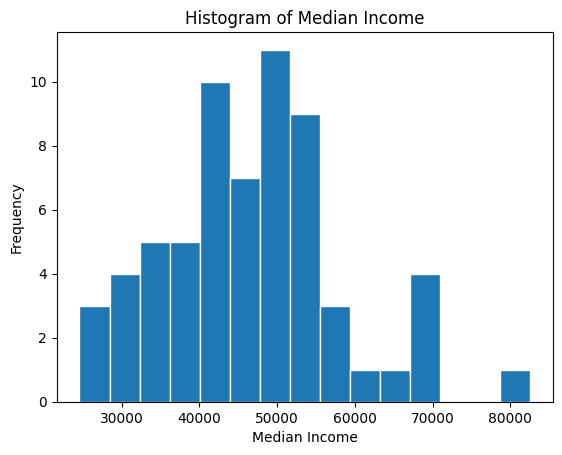
\includegraphics{labs/w03_webArch_files/figure-pdf/cell-11-output-1.png}

We can also explore correlations between variables. Let's use
\texttt{seaborn}.

\begin{Shaded}
\begin{Highlighting}[]
\ImportTok{import}\NormalTok{ seaborn }\ImportTok{as}\NormalTok{ sns}

\CommentTok{\# Creating a scatter plot with a linear regression line}
\NormalTok{sns.lmplot(x}\OperatorTok{=}\StringTok{\textquotesingle{}median\_age\textquotesingle{}}\NormalTok{, y}\OperatorTok{=}\StringTok{\textquotesingle{}median\_income\textquotesingle{}}\NormalTok{, data}\OperatorTok{=}\NormalTok{louisiana\_df, aspect}\OperatorTok{=}\FloatTok{1.5}\NormalTok{)}
\NormalTok{plt.xlabel(}\StringTok{\textquotesingle{}Median Age\textquotesingle{}}\NormalTok{)}
\NormalTok{plt.ylabel(}\StringTok{\textquotesingle{}Median Income\textquotesingle{}}\NormalTok{)}
\NormalTok{plt.title(}\StringTok{\textquotesingle{}Louisiana, Relationship between Income and Age\textquotesingle{}}\NormalTok{)}
\NormalTok{plt.show()}
\end{Highlighting}
\end{Shaded}

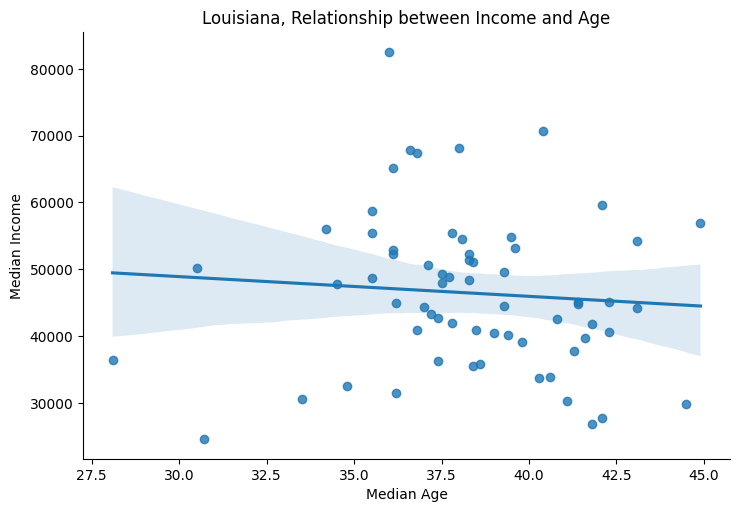
\includegraphics{labs/w03_webArch_files/figure-pdf/cell-12-output-1.png}

\textbf{Exercise}:

In pairs, modify the state, vairables and year parameters following the
approach adopted above and produce some other simple scatter plots
(cloud of points) that suggest correlations between your variables of
interest.

\section{Your own API request demo}\label{your-own-api-request-demo}

The Python libraries commonly used for API requests are
\texttt{requests} and \texttt{json}.

JSON stands for JavaScript Object Notation. Despite its association with
JavaScript, JSON is widely used due to its readability and ease of use
by computers, making it the primary format for data transmission through
APIs. Most APIs return their responses in JSON format. The \texttt{json}
library in Python allows you to parse and convert these JSON responses
into Python data structures. JSON structures are composed of key-value
pairs, similar to Python dictionaries.

In Python, to make an API request and handle the response, you would
typically use the the \texttt{requests} library. A standard API request
involves sending a \texttt{GET} request to the server's URL, which
specifies the data you wish to retrieve. For instance, to request the
locations of all the hire bike stations in London from the
\textbf{Transport for London} \href{https://api.tfl.gov.uk}{API}, you
would use the \texttt{requests.get()} method. This method requires a URL
that directs the request to the appropriate server.

\begin{Shaded}
\begin{Highlighting}[]
\ImportTok{import}\NormalTok{ requests}
\ImportTok{import}\NormalTok{ json}

\NormalTok{response }\OperatorTok{=}\NormalTok{ requests.get(}\StringTok{"https://api.tfl.gov.uk/BikePoint/"}\NormalTok{)}
\NormalTok{response}
\end{Highlighting}
\end{Shaded}

\begin{verbatim}
<Response [200]>
\end{verbatim}

Good! The response code 200 indicates a successful request

Most GET request URLs for API querying have three or four components:

\begin{enumerate}
\def\labelenumi{\arabic{enumi}.}
\tightlist
\item
  Authentication Key/Token: A user-specific character string appended to
  a base URL telling the server who is making the query; allows servers
  to efficiently manage database access.
\item
  Base URL: A link stub that will be at the beginning of all calls to a
  given API; points the server to the location of an entire database.
\item
  Search Parameters: A character string appended to a base URL that
  tells the server what to extract from the database; basically a series
  of filters used to point to specific parts of a database.
\item
  Response Format: A character string indicating how the response should
  be formatted; usually one of .csv, .json, or .xml.
\end{enumerate}

\begin{Shaded}
\begin{Highlighting}[]
\CommentTok{\# Making the API request}
\NormalTok{response }\OperatorTok{=}\NormalTok{ requests.get(}\StringTok{"https://api.tfl.gov.uk/BikePoint/"}\NormalTok{)}

\CommentTok{\# Parsing the response content as JSON and converting it to a DataFrame}
\NormalTok{bike\_stations }\OperatorTok{=}\NormalTok{ pd.DataFrame(response.json())}

\CommentTok{\# Printing the column names}
\BuiltInTok{print}\NormalTok{(bike\_stations.columns)}
\end{Highlighting}
\end{Shaded}

\begin{verbatim}
Index(['$type', 'id', 'url', 'commonName', 'placeType', 'additionalProperties',
       'children', 'childrenUrls', 'lat', 'lon'],
      dtype='object')
\end{verbatim}

\begin{Shaded}
\begin{Highlighting}[]
\CommentTok{\# Creating a new column \textquotesingle{}Station ID\textquotesingle{} by extracting the numeric part from the \textquotesingle{}id\textquotesingle{} column}
\NormalTok{bike\_stations[}\StringTok{\textquotesingle{}Station ID\textquotesingle{}}\NormalTok{] }\OperatorTok{=}\NormalTok{ bike\_stations[}\StringTok{\textquotesingle{}id\textquotesingle{}}\NormalTok{].}\BuiltInTok{str}\NormalTok{.extract(}\VerbatimStringTok{r\textquotesingle{}BikePoints\_(\textbackslash{}d+)\textquotesingle{}}\NormalTok{, expand}\OperatorTok{=}\VariableTok{False}\NormalTok{).astype(}\BuiltInTok{float}\NormalTok{)}
\NormalTok{bike\_stations.head()}
\end{Highlighting}
\end{Shaded}

\begin{longtable}[]{@{}llllllllllll@{}}
\toprule\noalign{}
& \$type & id & url & commonName & placeType & additionalProperties &
children & childrenUrls & lat & lon & Station ID \\
\midrule\noalign{}
\endhead
\bottomrule\noalign{}
\endlastfoot
0 & Tfl.Api.Presentation.Entities.Place, Tfl.Api.P... & BikePoints\_1 &
/Place/BikePoints\_1 & River Street , Clerkenwell & BikePoint &
{[}\{\textquotesingle\$type\textquotesingle:
\textquotesingle Tfl.Api.Presentation.Entities.Addi... & {[}{]} & {[}{]}
& 51.529163 & -0.109970 & 1.0 \\
1 & Tfl.Api.Presentation.Entities.Place, Tfl.Api.P... & BikePoints\_2 &
/Place/BikePoints\_2 & Phillimore Gardens, Kensington & BikePoint &
{[}\{\textquotesingle\$type\textquotesingle:
\textquotesingle Tfl.Api.Presentation.Entities.Addi... & {[}{]} & {[}{]}
& 51.499606 & -0.197574 & 2.0 \\
2 & Tfl.Api.Presentation.Entities.Place, Tfl.Api.P... & BikePoints\_3 &
/Place/BikePoints\_3 & Christopher Street, Liverpool Street & BikePoint
& {[}\{\textquotesingle\$type\textquotesingle:
\textquotesingle Tfl.Api.Presentation.Entities.Addi... & {[}{]} & {[}{]}
& 51.521283 & -0.084605 & 3.0 \\
3 & Tfl.Api.Presentation.Entities.Place, Tfl.Api.P... & BikePoints\_4 &
/Place/BikePoints\_4 & St. Chad\textquotesingle s Street,
King\textquotesingle s Cross & BikePoint &
{[}\{\textquotesingle\$type\textquotesingle:
\textquotesingle Tfl.Api.Presentation.Entities.Addi... & {[}{]} & {[}{]}
& 51.530059 & -0.120973 & 4.0 \\
4 & Tfl.Api.Presentation.Entities.Place, Tfl.Api.P... & BikePoints\_5 &
/Place/BikePoints\_5 & Sedding Street, Sloane Square & BikePoint &
{[}\{\textquotesingle\$type\textquotesingle:
\textquotesingle Tfl.Api.Presentation.Entities.Addi... & {[}{]} & {[}{]}
& 51.493130 & -0.156876 & 5.0 \\
\end{longtable}

By now you should be able to visualise the data that you have obtained
through this API.

\begin{Shaded}
\begin{Highlighting}[]
\OperatorTok{\%}\NormalTok{matplotlib inline}
\ImportTok{import}\NormalTok{ geopandas }\ImportTok{as}\NormalTok{ gpd}
\ImportTok{import}\NormalTok{ contextily }\ImportTok{as}\NormalTok{ ctx}

\CommentTok{\# Convert DataFrame to GeoDataFrame}
\NormalTok{gdf }\OperatorTok{=}\NormalTok{ gpd.GeoDataFrame(bike\_stations, geometry}\OperatorTok{=}\NormalTok{gpd.points\_from\_xy(bike\_stations.lon, bike\_stations.lat))}
\CommentTok{\# Setting the Coordinate Reference System (CRS) to WGS84 (EPSG:4326)}
\NormalTok{gdf.set\_crs(epsg}\OperatorTok{=}\DecValTok{4326}\NormalTok{, inplace}\OperatorTok{=}\VariableTok{True}\NormalTok{)}
\CommentTok{\# project to British Grid}
\NormalTok{gdf.to\_crs(epsg}\OperatorTok{=} \DecValTok{27700}\NormalTok{, inplace }\OperatorTok{=} \VariableTok{True}\NormalTok{)}

\CommentTok{\# Plotting bikepoints on a map}
\NormalTok{fig, ax }\OperatorTok{=}\NormalTok{ plt.subplots(}\DecValTok{1}\NormalTok{, }\DecValTok{1}\NormalTok{, figsize}\OperatorTok{=}\NormalTok{(}\DecValTok{8}\NormalTok{, }\DecValTok{6}\NormalTok{))}
\NormalTok{gdf.plot(ax }\OperatorTok{=}\NormalTok{ ax, color}\OperatorTok{=}\StringTok{\textquotesingle{}red\textquotesingle{}}\NormalTok{, markersize}\OperatorTok{=}\DecValTok{5}\NormalTok{)}
\NormalTok{source }\OperatorTok{=}\NormalTok{ ctx.providers.CartoDB.Positron}
\NormalTok{ctx.add\_basemap(ax, crs}\OperatorTok{=}\NormalTok{ gdf.crs.to\_string(), source}\OperatorTok{=}\NormalTok{ source)}
\NormalTok{ax.set\_title(}\StringTok{\textquotesingle{}Bike Points in London\textquotesingle{}}\NormalTok{)}
\end{Highlighting}
\end{Shaded}

\begin{verbatim}
Text(0.5, 1.0, 'Bike Points in London')
\end{verbatim}

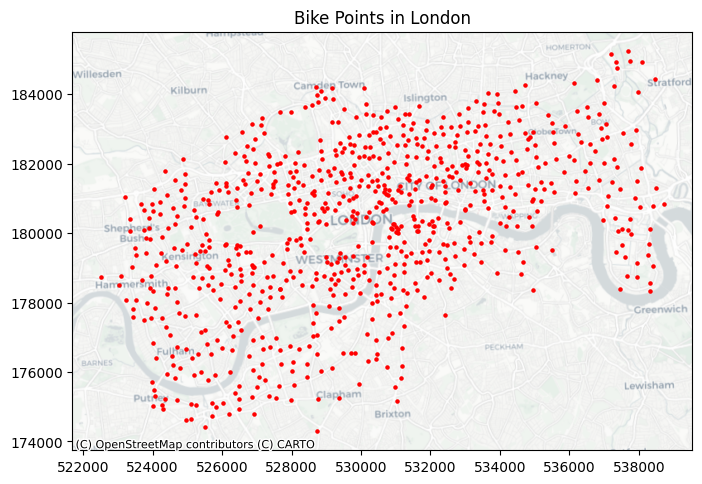
\includegraphics{labs/w03_webArch_files/figure-pdf/cell-16-output-2.png}

\section{Geocoding API}\label{geocoding-api}

Below is a short exploration of a the \texttt{geocoder} provided by the
library \texttt{geopy}. The \texttt{geocoder} relies on various external
geocoding services. When using \texttt{Nominatim}, it accesses data from
OpenStreetMap. OpenStreetMap's data includes a vast array of
geographical information sourced from contributors globally. This
includes street addresses, points of interest, and other location-based
data. When you provide an address to the Nominatim geocoder, it queries
OpenStreetMap's databases to find the corresponding geographical
coordinates.

In your own time, try to use it to automatically embed coordinates
between addresses.

\begin{Shaded}
\begin{Highlighting}[]
\ImportTok{from}\NormalTok{ geopy.geocoders }\ImportTok{import}\NormalTok{ Nominatim}

\CommentTok{\# Create a DataFrame with addresses}
\NormalTok{some\_addresses }\OperatorTok{=}\NormalTok{ pd.DataFrame(\{}
    \StringTok{\textquotesingle{}name\textquotesingle{}}\NormalTok{: [}\StringTok{"South Campus Teaching Hub"}\NormalTok{, }\StringTok{"Sefton Park"}\NormalTok{, }\StringTok{"Stanley Street"}\NormalTok{],}
    \StringTok{\textquotesingle{}addr\textquotesingle{}}\NormalTok{: [}\StringTok{"140 Chatham St, Liverpool L7 7BA"}\NormalTok{, }\StringTok{"Sefton Park, Liverpool L17 1AP"}\NormalTok{, }\StringTok{"4 Stanley St, Liverpool L1 6AA"}\NormalTok{]}
\NormalTok{\})}

\CommentTok{\# Initialize geocoder}
\NormalTok{geolocator }\OperatorTok{=}\NormalTok{ Nominatim(user\_agent}\OperatorTok{=}\StringTok{"geoapiExercises"}\NormalTok{)}

\CommentTok{\# Function for geocoding}
\KeywordTok{def}\NormalTok{ geocode(address):}
\NormalTok{    location }\OperatorTok{=}\NormalTok{ geolocator.geocode(address)}
    \ControlFlowTok{return}\NormalTok{ pd.Series([location.latitude, location.longitude], index}\OperatorTok{=}\NormalTok{[}\StringTok{\textquotesingle{}latitude\textquotesingle{}}\NormalTok{, }\StringTok{\textquotesingle{}longitude\textquotesingle{}}\NormalTok{])}

\CommentTok{\# Geocode the addresses}
\NormalTok{lat\_longs }\OperatorTok{=}\NormalTok{ some\_addresses[}\StringTok{\textquotesingle{}addr\textquotesingle{}}\NormalTok{].}\BuiltInTok{apply}\NormalTok{(geocode)}

\CommentTok{\# Adding the results back to the DataFrame}
\NormalTok{some\_addresses }\OperatorTok{=}\NormalTok{ some\_addresses.join(lat\_longs)}
\NormalTok{some\_addresses}
\end{Highlighting}
\end{Shaded}

\begin{longtable}[]{@{}lllll@{}}
\toprule\noalign{}
& name & addr & latitude & longitude \\
\midrule\noalign{}
\endhead
\bottomrule\noalign{}
\endlastfoot
0 & South Campus Teaching Hub & 140 Chatham St, Liverpool L7 7BA &
53.400188 & -2.964437 \\
1 & Sefton Park & Sefton Park, Liverpool L17 1AP & 53.389846 &
-2.923999 \\
2 & Stanley Street & 4 Stanley St, Liverpool L1 6AA & 53.407363 &
-2.987240 \\
\end{longtable}

\subsubsection{Reverse Geocoding}\label{reverse-geocoding}

You can also reverse geo-code the data, open the output and see what the
result is.

\begin{Shaded}
\begin{Highlighting}[]
\CommentTok{\# Reverse geocoding (optional)}
\KeywordTok{def}\NormalTok{ reverse\_geocode(lat, lon):}
\NormalTok{    location }\OperatorTok{=}\NormalTok{ geolocator.reverse((lat, lon))}
    \ControlFlowTok{return}\NormalTok{ location.address}

\CommentTok{\# Apply reverse geocoding}
\NormalTok{some\_addresses[[}\StringTok{\textquotesingle{}latitude\textquotesingle{}}\NormalTok{, }\StringTok{\textquotesingle{}longitude\textquotesingle{}}\NormalTok{]].}\BuiltInTok{apply}\NormalTok{(}\KeywordTok{lambda}\NormalTok{ x: reverse\_geocode(x[}\StringTok{\textquotesingle{}latitude\textquotesingle{}}\NormalTok{], x[}\StringTok{\textquotesingle{}longitude\textquotesingle{}}\NormalTok{]), axis}\OperatorTok{=}\DecValTok{1}\NormalTok{)}
\end{Highlighting}
\end{Shaded}

\begin{verbatim}
0    148, Chatham Street, Canning / Georgian Quarte...
1    Sefton Park, Smithdown Road, Wavertree, Liverp...
2    Davies Street, Cavern Quarter, Liverpool, Live...
dtype: object
\end{verbatim}

\subsubsection{Geographic Data through APIs and the
web}\label{geographic-data-through-apis-and-the-web}

APIs can help us generate and create spatial data. In this lab, we have
both:

\begin{itemize}
\tightlist
\item
  Written \textbf{our own API request.}
\item
  Used \textbf{Plug-n-play packages.}
\end{itemize}

There are many APIs where we can get data these days. A few other
examples include

\begin{itemize}
\tightlist
\item
  \href{https://data.london.gov.uk/developers/}{The London DataStore
  API}
\item
  \href{https://data.thameswater.co.uk/s/}{Thames Water API}
\item
  \href{https://www.londonair.org.uk/Londonair/API/}{London Air API}
\item
  \href{https://data.police.uk/docs/method/crime-street/}{Crime data}
\end{itemize}

\section{\texorpdfstring{\emph{Group activity
answers}}{Group activity answers}}\label{group-activity-answers}

\begin{enumerate}
\def\labelenumi{\arabic{enumi}.}
\item
  Uniform Resource Location (\texttt{URL}) is a string of characters
  that, when interpreted via the Hypertext Transfer Protocol
  (\texttt{HTTP}). URLs point to a data resource, notably files written
  in Hypertext Markup Language (\texttt{HTML}) or a subset of a
  database.

  \begin{itemize}
  \tightlist
  \item
    1xx informational response - the request was received, continuing
    process
  \item
    2xx successful - the request was successfully received, understood,
    and accepted
  \item
    3xx redirection - further action needs to be taken in order to
    complete the request
  \item
    4xx client error - the request contains bad syntax or cannot be
    fulfilled
  \item
    5xx server error - the server failed to fulfil an apparently valid
    request
  \end{itemize}
\item
  \texttt{GET} requests a representation of a data resource
  corresponding to a particular \texttt{URL}. The process of executing
  the \texttt{GET} method is often referred to as a
  \texttt{GET\ request} and is the main method used for querying RESTful
  databases. \texttt{HEAD}, \texttt{POST}, \texttt{PUT},
  \texttt{DELETE}: other common methods, though mostly never used for
  database querying.

  Surfing the web is basically equivalent to sending a bunch of
  \texttt{GET} requests to different servers and asking for different
  files written in \texttt{HTML}. Suppose, for instance, I wanted to
  look something up on Wikipedia. Your first step would be to open your
  web browser and type in http://www.wikipedia.org. Once you hit return,
  you would see the page below. Several different processes occured,
  however, between you hitting ``return'' and the page finally being
  rendered:

  \begin{enumerate}
  \def\labelenumii{\arabic{enumii}.}
  \tightlist
  \item
    The web browser took the entered character string, used the
    command-line tool ``Curl'' to write a properly formatted
    \texttt{HTTP\ GET} request, and submitted it to the server that
    hosts the Wikipedia homepage.
  \item
    After receiving this request, the server sent an \texttt{HTTP}
    response, from which \texttt{Curl} extracted the HTML code for the
    page (partially shown below).
  \item
    The raw \texttt{HTML} code was parsed and then executed by the web
    browser, rendering the page as seen in the window.
  \item
    Most APIs requires a key or other user credentials before you can
    query their database. Getting credentialised with a API requires
    that you register with the organization. Once you have successfully
    registered, you will be assigned one or more keys, tokens, or other
    credentials that must be supplied to the server as part of any API
    call you make. To make sure users are not abusing their data access
    privileges (e.g., by making many rapid queries), each set of keys
    will be given rate limits governing the total number of calls that
    can be made over certain intervals of time.
  \end{enumerate}
\item
  Most APIs requires a key before you can query their database. This
  usually requires you to register with the organization. Most APIs are
  set up for developers, so you will likely be asked to register an
  ``application.'' All this really entails is coming up with a name for
  your app/bot/project and providing your real name, organization, and
  email. Note that some more popular APIs (e.g., Twitter, Facebook) will
  require additional information, such as a web address or mobile
  number. Once you have registered, you will be assigned one or more
  keys, tokens, or other credentials that must be supplied to the server
  as part of any API call you make. Most API keys limits the total
  number of calls that can be made over certain intervals of time. This
  is so users do not busing their data access privileges.
\end{enumerate}

\section{References}\label{references-1}

\begin{itemize}
\tightlist
\item
  \href{https://www.internetsociety.org/resources/doc/2017/brief-history-internet/}{Brief
  History of the Internet}, by the Internet Society, is a handy (and
  free!) introduction to how it all came to be.
\item
  Haklay, M., Singleton, A., Parker, C. 2008.
  \href{https://compass.onlinelibrary.wiley.com/doi/abs/10.1111/j.1749-8198.2008.00167.x}{``Web
  Mapping 2.0: The Neogeography of the GeoWeb''}. Geography Compass,
  2(6):2011--2039
\item
  \href{https://joemorrison.medium.com/death-of-an-open-source-business-model-62bc227a7e9b}{A
  blog post from JoeMorrison} commenting on the recent change of
  licensing for some of the core software from Mapbox
\item
  Terman, R., 2020.
  \href{https://plsc-31101.github.io/course/}{Computational Tools for
  Social Science}
\end{itemize}

\bookmarksetup{startatroot}

\chapter{Data Architectures and
Tiles}\label{data-architectures-and-tiles}

The \textbf{Lecture slides} can be found
\href{https://github.com/GDSL-UL/wma/raw/main/lectures/w04.html}{here}.

In this lab, we will explore and familiarise with some of the most
common data formats for web mapping: GeoJSON and Mbtiles.

\section{GeoJSON}\label{geojson}

To get familiar with the format, we will start by creating a GeoJSON
file from scratch. Head over to the following website:

\url{https://geojson.io/}

In there, we will create together a small example to better understand
the building blocks of this file format.

We will pay special attention to the following aspects:

\begin{itemize}
\tightlist
\item
  Readability.
\item
  Coordinate system.
\item
  Ability to add non-spatial information attached to each record.
\item
  How to save it as a file.
\end{itemize}

\textbf{Excercise}:

Create a GeoJSON file for the following data and save them to separate
files:

\begin{enumerate}
\def\labelenumi{\arabic{enumi}.}
\tightlist
\item
  Your five favourite spots in Liverpool
\item
  A polygon of what you consider to be the boundary of the neighbourhood
  where you live and the city centre of Liverpool. Name each.
\item
  A route that captures one of your favorite walks around the Liverpool
  region
\end{enumerate}

If you are comfortable, upload the files to Microsoft Teams to share
them with peers.

\subsection{GeoJSON in Python}\label{geojson-in-python}

With the files from the exercise at hand, we will learn how to open them
in a Python environment. Then, let's begin by importing the necessary
libraries; \texttt{geojson}is used for handling GeoJSON files.

\begin{Shaded}
\begin{Highlighting}[]
\ImportTok{import}\NormalTok{ geopandas }\ImportTok{as}\NormalTok{ gpd}
\end{Highlighting}
\end{Shaded}

Now, place the .geojson files you have created in the data folder used
in these sessions. As always, the data folder should be stored in the
directory where the notebook is running from. For this example, we will
assume that the file is called \texttt{map.geojson}. We can read the
file as:

\begin{Shaded}
\begin{Highlighting}[]
\NormalTok{liverpool }\OperatorTok{=}\NormalTok{ gpd.read\_file(}\StringTok{"../data/map.geojson"}\NormalTok{)}
\NormalTok{liverpool.head()}
\end{Highlighting}
\end{Shaded}

We can also plot and explore the content of the GeoDataFrame with
\texttt{Folium}. Folium, which we will see more in detail later on,
helps create interactive maps from data stored in
\texttt{geopandas.GeoDataFrame}.

\begin{Shaded}
\begin{Highlighting}[]
\ImportTok{import}\NormalTok{ folium }

\NormalTok{liverpool\_centroid }\OperatorTok{=}\NormalTok{ (}\FloatTok{53.41058}\NormalTok{, }\OperatorTok{{-}}\FloatTok{2.97794}\NormalTok{)}
\CommentTok{\# Create a Folium map centered around this point}
\BuiltInTok{map} \OperatorTok{=}\NormalTok{ folium.Map(location}\OperatorTok{=}\NormalTok{liverpool\_centroid, zoom\_start}\OperatorTok{=}\DecValTok{13}\NormalTok{, tiles}\OperatorTok{=}\StringTok{"CartoDB.DarkMatterNoLabels"}\NormalTok{)}

\CommentTok{\# Add the liverpool data to the map, this will plot each geometry in the GeoDataFrame}
\NormalTok{folium.GeoJson(liverpool).add\_to(}\BuiltInTok{map}\NormalTok{)}
\BuiltInTok{map}
\end{Highlighting}
\end{Shaded}

Once read, the geojson behaves exactly like any GeoDataFrame we have
seen so far. We can therefore operate on it and tap into the
functionality from \texttt{pandas} and \texttt{geopandas}. For example,
we can and reproject the layer to the to British National Grid.

\begin{Shaded}
\begin{Highlighting}[]
\NormalTok{liverpool\_bng }\OperatorTok{=}\NormalTok{ liverpool.to\_crs(crs }\OperatorTok{=} \StringTok{"EPSG: 27700"}\NormalTok{)}
\end{Highlighting}
\end{Shaded}

When we inspected our geojson, we noted that the spatial data is stored
in the following format \texttt{POINT\ (-2.977367\ 53.40753)}. This is
called ``well known text'' (\texttt{wkt}) and is a representation that
spatial databases like PostGIS use as well. Another way to store spatial
data as text for storage or transfer, less (human) readable but more
efficient is the ``well known blurb'' (\texttt{wkb}). We can use the
\texttt{shapely} library to handle the WKT representation of the
geometry and then convert it to WKB format.

\begin{Shaded}
\begin{Highlighting}[]
\ImportTok{from}\NormalTok{ shapely }\ImportTok{import}\NormalTok{ wkt}
\ImportTok{from}\NormalTok{ shapely.geometry }\ImportTok{import}\NormalTok{ Point}
\ImportTok{import}\NormalTok{ shapely.wkb}

\CommentTok{\# Load the WKT representation of the point}
\NormalTok{wkt\_string }\OperatorTok{=} \StringTok{"POINT ({-}2.977367 53.40753)"}

\CommentTok{\# Convert the WKT representation into a Shapely Point object}
\NormalTok{point }\OperatorTok{=}\NormalTok{ wkt.loads(wkt\_string)}

\CommentTok{\# Convert the Point object into WKB format}
\NormalTok{wkb\_data }\OperatorTok{=}\NormalTok{ shapely.wkb.dumps(point)}
\NormalTok{wkb\_data.}\BuiltInTok{hex}\NormalTok{()}
\end{Highlighting}
\end{Shaded}

\textbf{Excercise}: - Read the \texttt{GeoJSON} created for your
favorite walks in Liverpool and calculate their length

Once you are happy with the data as we will hypothetically need it, you
can write it out to any other file format supported in
\texttt{geopandas}. For example, we can create a Geopackge file with the
same information. For this, we can use the function \texttt{to\_file}.
See an example below:

\begin{Shaded}
\begin{Highlighting}[]
\CommentTok{\# Write \textquotesingle{}liverpool\_bng\textquotesingle{} to a GeoPackage file}
\NormalTok{liverpool\_bng.to\_file(}\StringTok{"../data/liverpool\_bng.gpkg"}\NormalTok{, layer}\OperatorTok{=}\StringTok{"liverpool\_bng"}\NormalTok{, driver}\OperatorTok{=}\StringTok{"GPKG"}\NormalTok{)}
\end{Highlighting}
\end{Shaded}

\section{\texorpdfstring{Tilesets and
\texttt{Mbtiles}}{Tilesets and Mbtiles}}\label{tilesets-and-mbtiles}

In this section we will dive into the concept of tiles to understand why
they have been so transformative in the world of web mapping. We have
already seen the usage of tilesets above with \texttt{folium} and with
\texttt{contextily} (although within a static context). We will see that
\texttt{folium}, integrates different tileset options already.

For this section, let's start by getting the building footprints from
OpenStreetMap with \texttt{osmnx}

\begin{Shaded}
\begin{Highlighting}[]
\ImportTok{import}\NormalTok{ osmnx }\ImportTok{as}\NormalTok{ ox}
\NormalTok{tags }\OperatorTok{=}\NormalTok{ \{}\StringTok{"building"}\NormalTok{: }\VariableTok{True}\NormalTok{\} }\CommentTok{\#OSM tags}
\NormalTok{buildings }\OperatorTok{=}\NormalTok{ ox.features\_from\_place(}\StringTok{"Liverpool, UK"}\NormalTok{, tags }\OperatorTok{=}\NormalTok{ tags) }
\NormalTok{buildings }\OperatorTok{=}\NormalTok{ buildings.reset\_index()}
 \CommentTok{\# sometimes building footprints are represented by Points, let\textquotesingle{}s disregard them}
\NormalTok{buildings }\OperatorTok{=}\NormalTok{ buildings[(buildings.geometry.geom\_type }\OperatorTok{==} \StringTok{\textquotesingle{}Polygon\textquotesingle{}}\NormalTok{) }\OperatorTok{|}\NormalTok{ (buildings.geometry.geom\_type }\OperatorTok{==} \StringTok{\textquotesingle{}MultiPolygon\textquotesingle{}}\NormalTok{)]}
\end{Highlighting}
\end{Shaded}

\begin{Shaded}
\begin{Highlighting}[]
\NormalTok{buildings.plot()}
\end{Highlighting}
\end{Shaded}

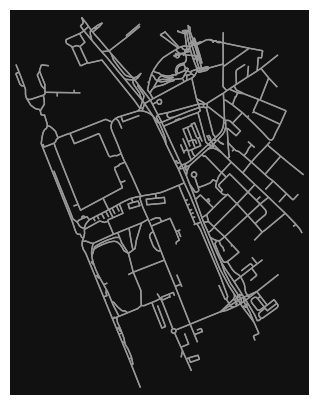
\includegraphics{labs/w04_dataArch_files/figure-pdf/cell-9-output-1.png}

Let's save the GeoDataFrame a geojson and call it
\texttt{buildings\_liverpool.geojson}.

\begin{Shaded}
\begin{Highlighting}[]
\NormalTok{buildings[[}\StringTok{\textquotesingle{}osmid\textquotesingle{}}\NormalTok{,}\StringTok{\textquotesingle{}geometry\textquotesingle{}}\NormalTok{]].to\_file(}\StringTok{\textquotesingle{}data/buildings\_liverpool.geojson\textquotesingle{}}\NormalTok{,  driver}\OperatorTok{=}\StringTok{\textquotesingle{}GeoJSON\textquotesingle{}}\NormalTok{)}
\end{Highlighting}
\end{Shaded}

Then, register for a MapBox account
\href{https://account.mapbox.com/auth/signup/?route-to=\%22https\%3A\%2F\%2Faccount.mapbox.com\%2Faccess-tokens\%2F\%22}{here}.

\subsection{Optional: Generating .mbtiles in
Python}\label{optional-generating-.mbtiles-in-python}

In Python, you can use \texttt{togeojsontiles} to make a dynamic
\texttt{.mbtiles} files. This is useful to visualize large data
appropriately at any zoom level. \textbf{This step cannot be ran on
University Machines} It requires the installation of \texttt{tippecanoe}
on your machine. Follow the corresponding instructions for
\href{https://gist.github.com/ryanbaumann/e5c7d76f6eeb8598e66c5785b677726e}{Windows}
and for \href{https://github.com/mapbox/tippecanoe}{MAC}

\begin{Shaded}
\begin{Highlighting}[]
\NormalTok{pip install togeojsontiles}
\ImportTok{from}\NormalTok{ togeojsontiles }\ImportTok{import}\NormalTok{ geojson\_to\_mbtiles}

\NormalTok{TIPPECANOE\_DIR }\OperatorTok{=} \StringTok{\textquotesingle{}/usr/local/bin/\textquotesingle{}}

\CommentTok{\# Convert GeoJSON to .mbtiles}
\NormalTok{togeojsontiles.geojson\_to\_mbtiles(}
\NormalTok{    filepaths}\OperatorTok{=}\NormalTok{[}\StringTok{\textquotesingle{}/data/buildings\_liverpool.geojson\textquotesingle{}}\NormalTok{],}
\NormalTok{    tippecanoe\_dir}\OperatorTok{=}\NormalTok{TIPPECANOE\_DIR,}
\NormalTok{    mbtiles\_file}\OperatorTok{=}\StringTok{\textquotesingle{}liverpool.mbtiles\textquotesingle{}}\NormalTok{,}
\NormalTok{    maxzoom}\OperatorTok{=}\DecValTok{14}\NormalTok{)}
\end{Highlighting}
\end{Shaded}

You can also try \textbf{uploading} it directly to Mapbox. This part of
the code has not been tested so it should serve as guidance.

\begin{Shaded}
\begin{Highlighting}[]
\ImportTok{import}\NormalTok{ requests}
\ImportTok{import}\NormalTok{ os}

\CommentTok{\# Define your Mapbox token}
\NormalTok{mapbox\_token }\OperatorTok{=} \StringTok{""}

\CommentTok{\# Endpoint for Mapbox Tiling Service uploads}
\NormalTok{url }\OperatorTok{=} \StringTok{\textquotesingle{}https://api.mapbox.com/uploads/v1/mapbox\textquotesingle{}}

\CommentTok{\# Path to your .mbtiles file}
\NormalTok{mbtiles\_file\_path }\OperatorTok{=} \StringTok{"../data/liverpool.mbtiles\textquotesingle{}}

\ErrorTok{\# Prepare the headers}
\NormalTok{headers }\OperatorTok{=}\NormalTok{ \{}
    \StringTok{\textquotesingle{}Authorization\textquotesingle{}}\NormalTok{: }\SpecialStringTok{f\textquotesingle{}Bearer }\SpecialCharTok{\{}\NormalTok{MAPBOX\_ACCESS\_TOKEN}\SpecialCharTok{\}}\SpecialStringTok{\textquotesingle{}}\NormalTok{,}
    \StringTok{\textquotesingle{}Content{-}Type\textquotesingle{}}\NormalTok{: }\StringTok{\textquotesingle{}application/json\textquotesingle{}}
\NormalTok{\}}

\CommentTok{\# Prepare the data for the POST request}
\ControlFlowTok{with} \BuiltInTok{open}\NormalTok{(mbtiles\_file\_path, }\StringTok{\textquotesingle{}rb\textquotesingle{}}\NormalTok{) }\ImportTok{as} \BuiltInTok{file}\NormalTok{:}
\NormalTok{    files }\OperatorTok{=}\NormalTok{ \{}\StringTok{\textquotesingle{}file\textquotesingle{}}\NormalTok{: }\BuiltInTok{file}\NormalTok{\}}
\NormalTok{    response }\OperatorTok{=}\NormalTok{ requests.post(url, headers}\OperatorTok{=}\NormalTok{headers, files}\OperatorTok{=}\NormalTok{files)}

\CommentTok{\# Check the response}
\ControlFlowTok{if}\NormalTok{ response.status\_code }\OperatorTok{==} \DecValTok{200}\NormalTok{:}
    \BuiltInTok{print}\NormalTok{(}\StringTok{"Upload initiated successfully."}\NormalTok{)}
    \BuiltInTok{print}\NormalTok{(response.json())}
\ControlFlowTok{else}\NormalTok{:}
    \BuiltInTok{print}\NormalTok{(}\StringTok{"Failed to initiate upload."}\NormalTok{)}
    \BuiltInTok{print}\NormalTok{(response.text)}
\end{Highlighting}
\end{Shaded}

\textbf{\emph{The optional steps end here}}

\subsection{\texorpdfstring{Uploading to \textbf{Mapbox
Studio}:}{Uploading to Mapbox Studio:}}\label{uploading-to-mapbox-studio}

After creating the \texttt{.mbtiles} file, you can upload it
\emph{manually} to Mapbox Studio (unless you managed to make the cell
above work):

\begin{itemize}
\tightlist
\item
  Navigate to Mapbox Studio.
\item
  Start a New Style and chose a template (Monochrome, blank etc.)
\end{itemize}

\begin{itemize}
\tightlist
\item
  Upload the \texttt{liverpool.mbtiles} (if you created it) or the
  \texttt{liverpool.geojson}. Press the \textbf{+} symbol,
  \texttt{Custom\ Layer} or \texttt{Data\ Visualisation},
  \texttt{Upload\ Data}, and choose your file
\end{itemize}

\begin{itemize}
\tightlist
\item
  Once uploaded, you should see your layer in the existing sources.
\end{itemize}

\begin{itemize}
\tightlist
\item
  Style it according to your requirements: It should look like a nicer
  version of this:
\end{itemize}

Or through \emph{scripting} with Mapbox's Uploads API (see above)

\subsection{\texorpdfstring{Visualizing the Tiles with
\texttt{Folium}:}{Visualizing the Tiles with Folium:}}\label{visualizing-the-tiles-with-folium}

First we need to get the \texttt{id} of your Mapbox style by copying its
url:

\emph{url example}:
\url{mapbox://styles/gabrif/clrpby9lc00a501pecacz8b7h}

the \texttt{style\_id} is the last section of the URL, in this case
\texttt{clrpby9lc00a501pecacz8b7h}

Then, we can use \texttt{folium}, which we will more in detail later on,
and use our tileset. Folium essentially allows us to create interactive
maps, usually starting from data stored in a \texttt{GeoDataFrame}.
While folium provides a series of built-in tilesets, here it is
demonstrated how to employ one's own.

\begin{Shaded}
\begin{Highlighting}[]
\CommentTok{\# Create a Folium map centered at a specific location}
\ImportTok{import}\NormalTok{ folium}

\NormalTok{mapbox\_user }\OperatorTok{=} \StringTok{\textquotesingle{}gabrif\textquotesingle{}}
\NormalTok{mapbox\_token }\OperatorTok{=} \StringTok{\textquotesingle{}\textquotesingle{}}
\NormalTok{style\_id }\OperatorTok{=} \StringTok{\textquotesingle{}clrpby9lc00a501pecacz8b7h\textquotesingle{}} 

\NormalTok{tiles }\OperatorTok{=} \StringTok{\textquotesingle{}https://api.mapbox.com/styles/v1/\textquotesingle{}}\OperatorTok{+}\NormalTok{mapbox\_user}\OperatorTok{+}\StringTok{\textquotesingle{}/\textquotesingle{}}\OperatorTok{+}\NormalTok{style\_id}\OperatorTok{+}\StringTok{\textquotesingle{}/tiles/256/}\SpecialCharTok{\{z\}}\StringTok{/}\SpecialCharTok{\{x\}}\StringTok{/}\SpecialCharTok{\{y\}}\StringTok{?access\_token=\textquotesingle{}}\OperatorTok{+}\NormalTok{mapbox\_token}
\BuiltInTok{map} \OperatorTok{=}\NormalTok{ folium.Map(location}\OperatorTok{=}\NormalTok{[}\FloatTok{53.406872}\NormalTok{, }\OperatorTok{{-}}\FloatTok{2.973286}\NormalTok{], zoom\_start}\OperatorTok{=}\DecValTok{14}\NormalTok{,}
\NormalTok{               tiles}\OperatorTok{=}\NormalTok{tiles,}
\NormalTok{               attr}\OperatorTok{=}\StringTok{\textquotesingle{}Mapbox\textquotesingle{}}\NormalTok{)}

\CommentTok{\# Display the map}
\BuiltInTok{map}
\end{Highlighting}
\end{Shaded}

\begin{verbatim}
<folium.folium.Map at 0x2b2b49b31d0>
\end{verbatim}

\bookmarksetup{startatroot}

\chapter{Interactive Maps}\label{interactive-maps}

The \textbf{Lecture slides} can be found
\href{https://github.com/GDSL-UL/wma/raw/main/lectures/w05.html}{here}.

\emph{Gabriele Filomena has readapted parts of this
\href{https://autogis-site.readthedocs.io/en/latest/lessons/lesson-5/interactive-maps.html}{notebook}}
to prepare this notebook. Copyright (c) Henrikki Tenkanen, Vuokko
Heikinheimo, Håvard Wallin Aagesen, Christoph Fink, Kamyar Hasanzadeh.

\href{https://link.springer.com/referenceworkentry/10.1007/978-3-319-23519-6_1485-2}{Online
maps} have been interactive for a long time: virtually all online maps
allow to zoom in and out, to pan the map extent, and to select map
features, or otherwise query information about them. Interactive content
in web pages, such as online maps, are typically implemented using
\href{https://en.wikipedia.org/wiki/ECMAScript}{\emph{JavaScript}/\emph{ECMAScript}},
a scripting language originally targeted at web pages, primarily, but
used for many otherapplications.

In the open source realm, there exists a number of different
\emph{JavaScript} libraries for interactive web cartography, including
\href{https://leafletjs.com/}{Leaflet} and
\href{https://openlayers.org/}{OpenLayers}. We will not write a single
line of \emph{JavaScript}; instead, we will take advantage of the
\href{https://python-visualization.github.io/folium/}{\emph{Folium}}
Python package: it helps create interactive \emph{Leaflet} maps from
data stored in \texttt{geopandas.GeoDataFrame}. Folium is a library that
bridges the capabilities of data manipulation in Python with the
interactive mapping strengths of Leaflet, a leading open-source
JavaScript library for creating dynamic, interactive maps in the
browser. Let's explore both Folium and Leaflet in more detail to
understand their roles and relationship.

\textbf{Leaflet} is at the heart of Folium's mapping capabilities. It's
an open-source JavaScript library used extensively in web mapping. Known
for its simplicity, performance, and ease of use, Leaflet has become a
popular choice among developers for embedding maps in web applications.
It allows users to create maps with various interactive features like
zooming, panning, markers, popups, and different layers.

\textbf{Folium} builds on Leaflet's foundation, bringing its interactive
mapping capabilities into the Python environment. This integration is
significant for several reasons:

\begin{itemize}
\tightlist
\item
  With Folium, Python users can use libraries like Pandas and directly
  create interactive Leaflet maps from within Python. This seamless
  integration means data can be manipulated, analyzed, and visualized
  using Python, without the need for extensive JavaScript knowledge.
\item
  Folium abstracts the complexity of Leaflet, allowing users to create
  sophisticated maps using simple Python commands.
\item
  Folium inherits Leaflet's interactivity, enabling the creation of
  feature-rich maps with various interactive elements such as markers,
  layers, and choropleths. These maps can be customized and embedded in
  web applications or Jupyter notebooks, making them highly versatile
  for data visualization tasks.
\item
  Folium can render maps with different tilesets (like OpenStreetMap,
  Stamen Terrain), overlay data in various formats, and even incorporate
  advanced features like heatmaps or GeoJSON layers.
\end{itemize}

Folium acts as a bridge between Python and Leaflet, enabling Python
users to incorporate and develop web maps within their environment. It
leverages Leaflet's core functionalities and extends them into the
Python ecosystem, making geospatial data visualization both powerful and
accessible within Python workflows.

\begin{quote}
Find more information about the capabilities of the \emph{Folium}
package on its official web pages: -
\href{https://python-visualization.github.io/folium/}{Documentation} -
\href{https://nbviewer.org/github/python-visualization/folium/tree/main/examples/}{Example
gallery} -
\href{https://python-visualization.github.io/folium/quickstart.html\#Getting-Started}{Quickstart
tutorial}
\end{quote}

\begin{Shaded}
\begin{Highlighting}[]
\ImportTok{import}\NormalTok{ folium}
\ImportTok{import}\NormalTok{ pandas }\ImportTok{as}\NormalTok{ pd}
\ImportTok{import}\NormalTok{ geopandas }\ImportTok{as}\NormalTok{ gpd}
\end{Highlighting}
\end{Shaded}

\section{Simple interactive web maps with
Folium}\label{simple-interactive-web-maps-with-folium}

We will start by creating a simple interactive web map that contains
nothing but a base map. This is so that we can get acustomed to how
Folium's syntax works, and which steps we have to take. We create a
\texttt{folium.Map} object, and specify centred around which
\texttt{location} and at which initial zoom level (\textasciitilde0-20)
a map shall be displayed. By setting \texttt{control\_scale} to
\texttt{True}, we make Folium display a scale bar.

\begin{Shaded}
\begin{Highlighting}[]
\NormalTok{location }\OperatorTok{=}\NormalTok{ (}\FloatTok{39.6508}\NormalTok{, }\FloatTok{66.9654}\NormalTok{) }\CommentTok{\# Samarkand, Uzbekistan}
\BuiltInTok{map} \OperatorTok{=}\NormalTok{ folium.Map(location}\OperatorTok{=}\NormalTok{location, zoom\_start}\OperatorTok{=}\DecValTok{13}\NormalTok{, control\_scale}\OperatorTok{=}\VariableTok{True}\NormalTok{)}
\BuiltInTok{map}
\end{Highlighting}
\end{Shaded}

\begin{verbatim}
<folium.folium.Map at 0x148ed64e650>
\end{verbatim}

\subsubsection{Save the resulting map}\label{save-the-resulting-map}

To save this map to an HTML file that can be opened in any web browser,
use \texttt{folium.Map.save()}:

\begin{Shaded}
\begin{Highlighting}[]
\BuiltInTok{map}\NormalTok{.save(}\StringTok{"base{-}map.html"}\NormalTok{)}
\end{Highlighting}
\end{Shaded}

\subsection{Basemap API}\label{basemap-api}

Folium, Leaflet.js and \texttt{contextily}, the library that we used for
adding basemaps to our static maps in the 2nd session, rely on built-in
tilesets borrowed from the
\href{https://github.com/geopandas/xyzservices}{\texttt{xyzservices}}
package. The XYZ protocol exposes maps as images for portions of the
Earth we will call tiles. The XYZ name stands from the ``coordinates''
used to locate a given tile. This of the entire planet split up into
squares, each of them available with a unique combination of X and Y
numbers. Now add a third one (Z) for the zoom level: lower values use
less tiles to cover the world, while higher resolution levels (higher Z)
will cover progressively smaller areas, but with more detail. Most XYZ
APIs expose tiles directly over HTTP, which means we can access them
from the browser.he attr keyword.

\begin{Shaded}
\begin{Highlighting}[]
\ImportTok{import}\NormalTok{ xyzservices.providers }\ImportTok{as}\NormalTok{ xyz}
\NormalTok{xyz}
\end{Highlighting}
\end{Shaded}

\begin{verbatim}
{'OpenStreetMap': {'Mapnik': {'url': 'https://tile.openstreetmap.org/{z}/{x}/{y}.png',
   'max_zoom': 19,
   'html_attribution': '&copy; <a href="https://www.openstreetmap.org/copyright">OpenStreetMap</a> contributors',
   'attribution': '(C) OpenStreetMap contributors',
   'name': 'OpenStreetMap.Mapnik'},
  'DE': {'url': 'https://tile.openstreetmap.de/{z}/{x}/{y}.png',
   'max_zoom': 18,
   'html_attribution': '&copy; <a href="https://www.openstreetmap.org/copyright">OpenStreetMap</a> contributors',
   'attribution': '(C) OpenStreetMap contributors',
   'name': 'OpenStreetMap.DE'},
  'CH': {'url': 'https://tile.osm.ch/switzerland/{z}/{x}/{y}.png',
   'max_zoom': 18,
   'html_attribution': '&copy; <a href="https://www.openstreetmap.org/copyright">OpenStreetMap</a> contributors',
   'attribution': '(C) OpenStreetMap contributors',
   'bounds': [[45, 5], [48, 11]],
   'name': 'OpenStreetMap.CH'},
  'France': {'url': 'https://{s}.tile.openstreetmap.fr/osmfr/{z}/{x}/{y}.png',
   'max_zoom': 20,
   'html_attribution': '&copy; OpenStreetMap France | &copy; <a href="https://www.openstreetmap.org/copyright">OpenStreetMap</a> contributors',
   'attribution': '(C) OpenStreetMap France | (C) OpenStreetMap contributors',
   'name': 'OpenStreetMap.France'},
  'HOT': {'url': 'https://{s}.tile.openstreetmap.fr/hot/{z}/{x}/{y}.png',
   'max_zoom': 19,
   'html_attribution': '&copy; <a href="https://www.openstreetmap.org/copyright">OpenStreetMap</a> contributors, Tiles style by <a href="https://www.hotosm.org/" target="_blank">Humanitarian OpenStreetMap Team</a> hosted by <a href="https://openstreetmap.fr/" target="_blank">OpenStreetMap France</a>',
   'attribution': '(C) OpenStreetMap contributors, Tiles style by Humanitarian OpenStreetMap Team hosted by OpenStreetMap France',
   'name': 'OpenStreetMap.HOT'},
  'BZH': {'url': 'https://tile.openstreetmap.bzh/br/{z}/{x}/{y}.png',
   'max_zoom': 19,
   'html_attribution': '&copy; <a href="https://www.openstreetmap.org/copyright">OpenStreetMap</a> contributors, Tiles courtesy of <a href="http://www.openstreetmap.bzh/" target="_blank">Breton OpenStreetMap Team</a>',
   'attribution': '(C) OpenStreetMap contributors, Tiles courtesy of Breton OpenStreetMap Team',
   'bounds': [[46.2, -5.5], [50, 0.7]],
   'name': 'OpenStreetMap.BZH'},
  'BlackAndWhite': {'url': 'http://{s}.tiles.wmflabs.org/bw-mapnik/{z}/{x}/{y}.png',
   'max_zoom': 18,
   'attribution': '(C) OpenStreetMap contributors',
   'html_attribution': '&copy; <a href="https://www.openstreetmap.org/copyright">OpenStreetMap</a> contributors',
   'name': 'OpenStreetMap.BlackAndWhite'}},
 'MapTilesAPI': {'OSMEnglish': {'url': 'https://maptiles.p.rapidapi.com/{variant}/{z}/{x}/{y}.png?rapidapi-key={apikey}',
   'html_attribution': '&copy; <a href="http://www.maptilesapi.com/">MapTiles API</a>, &copy; <a href="https://www.openstreetmap.org/copyright">OpenStreetMap</a> contributors',
   'attribution': '(C) MapTiles API, (C) OpenStreetMap contributors',
   'variant': 'en/map/v1',
   'apikey': '<insert your api key here>',
   'max_zoom': 19,
   'name': 'MapTilesAPI.OSMEnglish'},
  'OSMFrancais': {'url': 'https://maptiles.p.rapidapi.com/{variant}/{z}/{x}/{y}.png?rapidapi-key={apikey}',
   'html_attribution': '&copy; <a href="http://www.maptilesapi.com/">MapTiles API</a>, &copy; <a href="https://www.openstreetmap.org/copyright">OpenStreetMap</a> contributors',
   'attribution': '(C) MapTiles API, (C) OpenStreetMap contributors',
   'variant': 'fr/map/v1',
   'apikey': '<insert your api key here>',
   'max_zoom': 19,
   'name': 'MapTilesAPI.OSMFrancais'},
  'OSMEspagnol': {'url': 'https://maptiles.p.rapidapi.com/{variant}/{z}/{x}/{y}.png?rapidapi-key={apikey}',
   'html_attribution': '&copy; <a href="http://www.maptilesapi.com/">MapTiles API</a>, &copy; <a href="https://www.openstreetmap.org/copyright">OpenStreetMap</a> contributors',
   'attribution': '(C) MapTiles API, (C) OpenStreetMap contributors',
   'variant': 'es/map/v1',
   'apikey': '<insert your api key here>',
   'max_zoom': 19,
   'name': 'MapTilesAPI.OSMEspagnol'}},
 'OpenSeaMap': {'url': 'https://tiles.openseamap.org/seamark/{z}/{x}/{y}.png',
  'html_attribution': 'Map data: &copy; <a href="http://www.openseamap.org">OpenSeaMap</a> contributors',
  'attribution': 'Map data: (C) OpenSeaMap contributors',
  'name': 'OpenSeaMap'},
 'OPNVKarte': {'url': 'https://tileserver.memomaps.de/tilegen/{z}/{x}/{y}.png',
  'max_zoom': 18,
  'html_attribution': 'Map <a href="https://memomaps.de/">memomaps.de</a> <a href="http://creativecommons.org/licenses/by-sa/2.0/">CC-BY-SA</a>, map data &copy; <a href="https://www.openstreetmap.org/copyright">OpenStreetMap</a> contributors',
  'attribution': 'Map memomaps.de CC-BY-SA, map data (C) OpenStreetMap contributors',
  'name': 'OPNVKarte'},
 'OpenTopoMap': {'url': 'https://{s}.tile.opentopomap.org/{z}/{x}/{y}.png',
  'max_zoom': 17,
  'html_attribution': 'Map data: &copy; <a href="https://www.openstreetmap.org/copyright">OpenStreetMap</a> contributors, <a href="http://viewfinderpanoramas.org">SRTM</a> | Map style: &copy; <a href="https://opentopomap.org">OpenTopoMap</a> (<a href="https://creativecommons.org/licenses/by-sa/3.0/">CC-BY-SA</a>)',
  'attribution': 'Map data: (C) OpenStreetMap contributors, SRTM | Map style: (C) OpenTopoMap (CC-BY-SA)',
  'name': 'OpenTopoMap'},
 'OpenRailwayMap': {'url': 'https://{s}.tiles.openrailwaymap.org/standard/{z}/{x}/{y}.png',
  'max_zoom': 19,
  'html_attribution': 'Map data: &copy; <a href="https://www.openstreetmap.org/copyright">OpenStreetMap</a> contributors | Map style: &copy; <a href="https://www.OpenRailwayMap.org">OpenRailwayMap</a> (<a href="https://creativecommons.org/licenses/by-sa/3.0/">CC-BY-SA</a>)',
  'attribution': 'Map data: (C) OpenStreetMap contributors | Map style: (C) OpenRailwayMap (CC-BY-SA)',
  'name': 'OpenRailwayMap'},
 'OpenFireMap': {'url': 'http://openfiremap.org/hytiles/{z}/{x}/{y}.png',
  'max_zoom': 19,
  'html_attribution': 'Map data: &copy; <a href="https://www.openstreetmap.org/copyright">OpenStreetMap</a> contributors | Map style: &copy; <a href="http://www.openfiremap.org">OpenFireMap</a> (<a href="https://creativecommons.org/licenses/by-sa/3.0/">CC-BY-SA</a>)',
  'attribution': 'Map data: (C) OpenStreetMap contributors | Map style: (C) OpenFireMap (CC-BY-SA)',
  'name': 'OpenFireMap'},
 'SafeCast': {'url': 'https://s3.amazonaws.com/te512.safecast.org/{z}/{x}/{y}.png',
  'max_zoom': 16,
  'html_attribution': 'Map data: &copy; <a href="https://www.openstreetmap.org/copyright">OpenStreetMap</a> contributors | Map style: &copy; <a href="https://blog.safecast.org/about/">SafeCast</a> (<a href="https://creativecommons.org/licenses/by-sa/3.0/">CC-BY-SA</a>)',
  'attribution': 'Map data: (C) OpenStreetMap contributors | Map style: (C) SafeCast (CC-BY-SA)',
  'name': 'SafeCast'},
 'Stadia': {'AlidadeSmooth': {'url': 'https://tiles.stadiamaps.com/tiles/{variant}/{z}/{x}/{y}{r}.{ext}',
   'min_zoom': 0,
   'max_zoom': 20,
   'html_attribution': '&copy; <a href="https://www.stadiamaps.com/" target="_blank">Stadia Maps</a> &copy; <a href="https://openmaptiles.org/" target="_blank">OpenMapTiles</a> &copy; <a href="https://www.openstreetmap.org/copyright">OpenStreetMap</a> contributors',
   'attribution': '(C) Stadia Maps (C) OpenMapTiles (C) OpenStreetMap contributors',
   'variant': 'alidade_smooth',
   'ext': 'png',
   'name': 'Stadia.AlidadeSmooth'},
  'AlidadeSmoothDark': {'url': 'https://tiles.stadiamaps.com/tiles/{variant}/{z}/{x}/{y}{r}.{ext}',
   'min_zoom': 0,
   'max_zoom': 20,
   'html_attribution': '&copy; <a href="https://www.stadiamaps.com/" target="_blank">Stadia Maps</a> &copy; <a href="https://openmaptiles.org/" target="_blank">OpenMapTiles</a> &copy; <a href="https://www.openstreetmap.org/copyright">OpenStreetMap</a> contributors',
   'attribution': '(C) Stadia Maps (C) OpenMapTiles (C) OpenStreetMap contributors',
   'variant': 'alidade_smooth_dark',
   'ext': 'png',
   'name': 'Stadia.AlidadeSmoothDark'},
  'OSMBright': {'url': 'https://tiles.stadiamaps.com/tiles/{variant}/{z}/{x}/{y}{r}.{ext}',
   'min_zoom': 0,
   'max_zoom': 20,
   'html_attribution': '&copy; <a href="https://www.stadiamaps.com/" target="_blank">Stadia Maps</a> &copy; <a href="https://openmaptiles.org/" target="_blank">OpenMapTiles</a> &copy; <a href="https://www.openstreetmap.org/copyright">OpenStreetMap</a> contributors',
   'attribution': '(C) Stadia Maps (C) OpenMapTiles (C) OpenStreetMap contributors',
   'variant': 'osm_bright',
   'ext': 'png',
   'name': 'Stadia.OSMBright'},
  'Outdoors': {'url': 'https://tiles.stadiamaps.com/tiles/{variant}/{z}/{x}/{y}{r}.{ext}',
   'min_zoom': 0,
   'max_zoom': 20,
   'html_attribution': '&copy; <a href="https://www.stadiamaps.com/" target="_blank">Stadia Maps</a> &copy; <a href="https://openmaptiles.org/" target="_blank">OpenMapTiles</a> &copy; <a href="https://www.openstreetmap.org/copyright">OpenStreetMap</a> contributors',
   'attribution': '(C) Stadia Maps (C) OpenMapTiles (C) OpenStreetMap contributors',
   'variant': 'outdoors',
   'ext': 'png',
   'name': 'Stadia.Outdoors'},
  'StamenToner': {'url': 'https://tiles.stadiamaps.com/tiles/{variant}/{z}/{x}/{y}{r}.{ext}',
   'min_zoom': 0,
   'max_zoom': 20,
   'html_attribution': '&copy; <a href="https://www.stadiamaps.com/" target="_blank">Stadia Maps</a> &copy; <a href="https://www.stamen.com/" target="_blank">Stamen Design</a> &copy; <a href="https://openmaptiles.org/" target="_blank">OpenMapTiles</a> &copy; <a href="https://www.openstreetmap.org/copyright">OpenStreetMap</a> contributors',
   'attribution': '(C) Stadia Maps (C) Stamen Design (C) OpenMapTiles (C) OpenStreetMap contributors',
   'variant': 'stamen_toner',
   'ext': 'png',
   'name': 'Stadia.StamenToner'},
  'StamenTonerBackground': {'url': 'https://tiles.stadiamaps.com/tiles/{variant}/{z}/{x}/{y}{r}.{ext}',
   'min_zoom': 0,
   'max_zoom': 20,
   'html_attribution': '&copy; <a href="https://www.stadiamaps.com/" target="_blank">Stadia Maps</a> &copy; <a href="https://www.stamen.com/" target="_blank">Stamen Design</a> &copy; <a href="https://openmaptiles.org/" target="_blank">OpenMapTiles</a> &copy; <a href="https://www.openstreetmap.org/copyright">OpenStreetMap</a> contributors',
   'attribution': '(C) Stadia Maps (C) Stamen Design (C) OpenMapTiles (C) OpenStreetMap contributors',
   'variant': 'stamen_toner_background',
   'ext': 'png',
   'name': 'Stadia.StamenTonerBackground'},
  'StamenTonerLines': {'url': 'https://tiles.stadiamaps.com/tiles/{variant}/{z}/{x}/{y}{r}.{ext}',
   'min_zoom': 0,
   'max_zoom': 20,
   'html_attribution': '&copy; <a href="https://www.stadiamaps.com/" target="_blank">Stadia Maps</a> &copy; <a href="https://www.stamen.com/" target="_blank">Stamen Design</a> &copy; <a href="https://openmaptiles.org/" target="_blank">OpenMapTiles</a> &copy; <a href="https://www.openstreetmap.org/copyright">OpenStreetMap</a> contributors',
   'attribution': '(C) Stadia Maps (C) Stamen Design (C) OpenMapTiles (C) OpenStreetMap contributors',
   'variant': 'stamen_toner_lines',
   'ext': 'png',
   'name': 'Stadia.StamenTonerLines'},
  'StamenTonerLabels': {'url': 'https://tiles.stadiamaps.com/tiles/{variant}/{z}/{x}/{y}{r}.{ext}',
   'min_zoom': 0,
   'max_zoom': 20,
   'html_attribution': '&copy; <a href="https://www.stadiamaps.com/" target="_blank">Stadia Maps</a> &copy; <a href="https://www.stamen.com/" target="_blank">Stamen Design</a> &copy; <a href="https://openmaptiles.org/" target="_blank">OpenMapTiles</a> &copy; <a href="https://www.openstreetmap.org/copyright">OpenStreetMap</a> contributors',
   'attribution': '(C) Stadia Maps (C) Stamen Design (C) OpenMapTiles (C) OpenStreetMap contributors',
   'variant': 'stamen_toner_labels',
   'ext': 'png',
   'name': 'Stadia.StamenTonerLabels'},
  'StamenTonerLite': {'url': 'https://tiles.stadiamaps.com/tiles/{variant}/{z}/{x}/{y}{r}.{ext}',
   'min_zoom': 0,
   'max_zoom': 20,
   'html_attribution': '&copy; <a href="https://www.stadiamaps.com/" target="_blank">Stadia Maps</a> &copy; <a href="https://www.stamen.com/" target="_blank">Stamen Design</a> &copy; <a href="https://openmaptiles.org/" target="_blank">OpenMapTiles</a> &copy; <a href="https://www.openstreetmap.org/copyright">OpenStreetMap</a> contributors',
   'attribution': '(C) Stadia Maps (C) Stamen Design (C) OpenMapTiles (C) OpenStreetMap contributors',
   'variant': 'stamen_toner_lite',
   'ext': 'png',
   'name': 'Stadia.StamenTonerLite'},
  'StamenWatercolor': {'url': 'https://tiles.stadiamaps.com/tiles/{variant}/{z}/{x}/{y}.{ext}',
   'min_zoom': 1,
   'max_zoom': 16,
   'html_attribution': '&copy; <a href="https://www.stadiamaps.com/" target="_blank">Stadia Maps</a> &copy; <a href="https://www.stamen.com/" target="_blank">Stamen Design</a> &copy; <a href="https://openmaptiles.org/" target="_blank">OpenMapTiles</a> &copy; <a href="https://www.openstreetmap.org/copyright">OpenStreetMap</a> contributors',
   'attribution': '(C) Stadia Maps (C) Stamen Design (C) OpenMapTiles (C) OpenStreetMap contributors',
   'variant': 'stamen_watercolor',
   'ext': 'jpg',
   'name': 'Stadia.StamenWatercolor'},
  'StamenTerrain': {'url': 'https://tiles.stadiamaps.com/tiles/{variant}/{z}/{x}/{y}{r}.{ext}',
   'min_zoom': 0,
   'max_zoom': 18,
   'html_attribution': '&copy; <a href="https://www.stadiamaps.com/" target="_blank">Stadia Maps</a> &copy; <a href="https://www.stamen.com/" target="_blank">Stamen Design</a> &copy; <a href="https://openmaptiles.org/" target="_blank">OpenMapTiles</a> &copy; <a href="https://www.openstreetmap.org/copyright">OpenStreetMap</a> contributors',
   'attribution': '(C) Stadia Maps (C) Stamen Design (C) OpenMapTiles (C) OpenStreetMap contributors',
   'variant': 'stamen_terrain',
   'ext': 'png',
   'name': 'Stadia.StamenTerrain'},
  'StamenTerrainBackground': {'url': 'https://tiles.stadiamaps.com/tiles/{variant}/{z}/{x}/{y}{r}.{ext}',
   'min_zoom': 0,
   'max_zoom': 18,
   'html_attribution': '&copy; <a href="https://www.stadiamaps.com/" target="_blank">Stadia Maps</a> &copy; <a href="https://www.stamen.com/" target="_blank">Stamen Design</a> &copy; <a href="https://openmaptiles.org/" target="_blank">OpenMapTiles</a> &copy; <a href="https://www.openstreetmap.org/copyright">OpenStreetMap</a> contributors',
   'attribution': '(C) Stadia Maps (C) Stamen Design (C) OpenMapTiles (C) OpenStreetMap contributors',
   'variant': 'stamen_terrain_background',
   'ext': 'png',
   'name': 'Stadia.StamenTerrainBackground'},
  'StamenTerrainLabels': {'url': 'https://tiles.stadiamaps.com/tiles/{variant}/{z}/{x}/{y}{r}.{ext}',
   'min_zoom': 0,
   'max_zoom': 18,
   'html_attribution': '&copy; <a href="https://www.stadiamaps.com/" target="_blank">Stadia Maps</a> &copy; <a href="https://www.stamen.com/" target="_blank">Stamen Design</a> &copy; <a href="https://openmaptiles.org/" target="_blank">OpenMapTiles</a> &copy; <a href="https://www.openstreetmap.org/copyright">OpenStreetMap</a> contributors',
   'attribution': '(C) Stadia Maps (C) Stamen Design (C) OpenMapTiles (C) OpenStreetMap contributors',
   'variant': 'stamen_terrain_labels',
   'ext': 'png',
   'name': 'Stadia.StamenTerrainLabels'},
  'StamenTerrainLines': {'url': 'https://tiles.stadiamaps.com/tiles/{variant}/{z}/{x}/{y}{r}.{ext}',
   'min_zoom': 0,
   'max_zoom': 18,
   'html_attribution': '&copy; <a href="https://www.stadiamaps.com/" target="_blank">Stadia Maps</a> &copy; <a href="https://www.stamen.com/" target="_blank">Stamen Design</a> &copy; <a href="https://openmaptiles.org/" target="_blank">OpenMapTiles</a> &copy; <a href="https://www.openstreetmap.org/copyright">OpenStreetMap</a> contributors',
   'attribution': '(C) Stadia Maps (C) Stamen Design (C) OpenMapTiles (C) OpenStreetMap contributors',
   'variant': 'stamen_terrain_lines',
   'ext': 'png',
   'name': 'Stadia.StamenTerrainLines'}},
 'Thunderforest': {'OpenCycleMap': {'url': 'https://{s}.tile.thunderforest.com/{variant}/{z}/{x}/{y}.png?apikey={apikey}',
   'html_attribution': '&copy; <a href="http://www.thunderforest.com/">Thunderforest</a>, &copy; <a href="https://www.openstreetmap.org/copyright">OpenStreetMap</a> contributors',
   'attribution': '(C) Thunderforest, (C) OpenStreetMap contributors',
   'variant': 'cycle',
   'apikey': '<insert your api key here>',
   'max_zoom': 22,
   'name': 'Thunderforest.OpenCycleMap'},
  'Transport': {'url': 'https://{s}.tile.thunderforest.com/{variant}/{z}/{x}/{y}.png?apikey={apikey}',
   'html_attribution': '&copy; <a href="http://www.thunderforest.com/">Thunderforest</a>, &copy; <a href="https://www.openstreetmap.org/copyright">OpenStreetMap</a> contributors',
   'attribution': '(C) Thunderforest, (C) OpenStreetMap contributors',
   'variant': 'transport',
   'apikey': '<insert your api key here>',
   'max_zoom': 22,
   'name': 'Thunderforest.Transport'},
  'TransportDark': {'url': 'https://{s}.tile.thunderforest.com/{variant}/{z}/{x}/{y}.png?apikey={apikey}',
   'html_attribution': '&copy; <a href="http://www.thunderforest.com/">Thunderforest</a>, &copy; <a href="https://www.openstreetmap.org/copyright">OpenStreetMap</a> contributors',
   'attribution': '(C) Thunderforest, (C) OpenStreetMap contributors',
   'variant': 'transport-dark',
   'apikey': '<insert your api key here>',
   'max_zoom': 22,
   'name': 'Thunderforest.TransportDark'},
  'SpinalMap': {'url': 'https://{s}.tile.thunderforest.com/{variant}/{z}/{x}/{y}.png?apikey={apikey}',
   'html_attribution': '&copy; <a href="http://www.thunderforest.com/">Thunderforest</a>, &copy; <a href="https://www.openstreetmap.org/copyright">OpenStreetMap</a> contributors',
   'attribution': '(C) Thunderforest, (C) OpenStreetMap contributors',
   'variant': 'spinal-map',
   'apikey': '<insert your api key here>',
   'max_zoom': 22,
   'name': 'Thunderforest.SpinalMap'},
  'Landscape': {'url': 'https://{s}.tile.thunderforest.com/{variant}/{z}/{x}/{y}.png?apikey={apikey}',
   'html_attribution': '&copy; <a href="http://www.thunderforest.com/">Thunderforest</a>, &copy; <a href="https://www.openstreetmap.org/copyright">OpenStreetMap</a> contributors',
   'attribution': '(C) Thunderforest, (C) OpenStreetMap contributors',
   'variant': 'landscape',
   'apikey': '<insert your api key here>',
   'max_zoom': 22,
   'name': 'Thunderforest.Landscape'},
  'Outdoors': {'url': 'https://{s}.tile.thunderforest.com/{variant}/{z}/{x}/{y}.png?apikey={apikey}',
   'html_attribution': '&copy; <a href="http://www.thunderforest.com/">Thunderforest</a>, &copy; <a href="https://www.openstreetmap.org/copyright">OpenStreetMap</a> contributors',
   'attribution': '(C) Thunderforest, (C) OpenStreetMap contributors',
   'variant': 'outdoors',
   'apikey': '<insert your api key here>',
   'max_zoom': 22,
   'name': 'Thunderforest.Outdoors'},
  'Pioneer': {'url': 'https://{s}.tile.thunderforest.com/{variant}/{z}/{x}/{y}.png?apikey={apikey}',
   'html_attribution': '&copy; <a href="http://www.thunderforest.com/">Thunderforest</a>, &copy; <a href="https://www.openstreetmap.org/copyright">OpenStreetMap</a> contributors',
   'attribution': '(C) Thunderforest, (C) OpenStreetMap contributors',
   'variant': 'pioneer',
   'apikey': '<insert your api key here>',
   'max_zoom': 22,
   'name': 'Thunderforest.Pioneer'},
  'MobileAtlas': {'url': 'https://{s}.tile.thunderforest.com/{variant}/{z}/{x}/{y}.png?apikey={apikey}',
   'html_attribution': '&copy; <a href="http://www.thunderforest.com/">Thunderforest</a>, &copy; <a href="https://www.openstreetmap.org/copyright">OpenStreetMap</a> contributors',
   'attribution': '(C) Thunderforest, (C) OpenStreetMap contributors',
   'variant': 'mobile-atlas',
   'apikey': '<insert your api key here>',
   'max_zoom': 22,
   'name': 'Thunderforest.MobileAtlas'},
  'Neighbourhood': {'url': 'https://{s}.tile.thunderforest.com/{variant}/{z}/{x}/{y}.png?apikey={apikey}',
   'html_attribution': '&copy; <a href="http://www.thunderforest.com/">Thunderforest</a>, &copy; <a href="https://www.openstreetmap.org/copyright">OpenStreetMap</a> contributors',
   'attribution': '(C) Thunderforest, (C) OpenStreetMap contributors',
   'variant': 'neighbourhood',
   'apikey': '<insert your api key here>',
   'max_zoom': 22,
   'name': 'Thunderforest.Neighbourhood'}},
 'CyclOSM': {'url': 'https://{s}.tile-cyclosm.openstreetmap.fr/cyclosm/{z}/{x}/{y}.png',
  'max_zoom': 20,
  'html_attribution': '<a href="https://github.com/cyclosm/cyclosm-cartocss-style/releases" title="CyclOSM - Open Bicycle render">CyclOSM</a> | Map data: &copy; <a href="https://www.openstreetmap.org/copyright">OpenStreetMap</a> contributors',
  'attribution': 'CyclOSM | Map data: (C) OpenStreetMap contributors',
  'name': 'CyclOSM'},
 'Jawg': {'Streets': {'url': 'https://{s}.tile.jawg.io/{variant}/{z}/{x}/{y}{r}.png?access-token={accessToken}',
   'html_attribution': '<a href="http://jawg.io" title="Tiles Courtesy of Jawg Maps" target="_blank">&copy; <b>Jawg</b>Maps</a> &copy; <a href="https://www.openstreetmap.org/copyright">OpenStreetMap</a> contributors',
   'attribution': '(C) **Jawg** Maps (C) OpenStreetMap contributors',
   'min_zoom': 0,
   'max_zoom': 22,
   'subdomains': 'abcd',
   'variant': 'jawg-streets',
   'accessToken': '<insert your access token here>',
   'name': 'Jawg.Streets'},
  'Terrain': {'url': 'https://{s}.tile.jawg.io/{variant}/{z}/{x}/{y}{r}.png?access-token={accessToken}',
   'html_attribution': '<a href="http://jawg.io" title="Tiles Courtesy of Jawg Maps" target="_blank">&copy; <b>Jawg</b>Maps</a> &copy; <a href="https://www.openstreetmap.org/copyright">OpenStreetMap</a> contributors',
   'attribution': '(C) **Jawg** Maps (C) OpenStreetMap contributors',
   'min_zoom': 0,
   'max_zoom': 22,
   'subdomains': 'abcd',
   'variant': 'jawg-terrain',
   'accessToken': '<insert your access token here>',
   'name': 'Jawg.Terrain'},
  'Sunny': {'url': 'https://{s}.tile.jawg.io/{variant}/{z}/{x}/{y}{r}.png?access-token={accessToken}',
   'html_attribution': '<a href="http://jawg.io" title="Tiles Courtesy of Jawg Maps" target="_blank">&copy; <b>Jawg</b>Maps</a> &copy; <a href="https://www.openstreetmap.org/copyright">OpenStreetMap</a> contributors',
   'attribution': '(C) **Jawg** Maps (C) OpenStreetMap contributors',
   'min_zoom': 0,
   'max_zoom': 22,
   'subdomains': 'abcd',
   'variant': 'jawg-sunny',
   'accessToken': '<insert your access token here>',
   'name': 'Jawg.Sunny'},
  'Dark': {'url': 'https://{s}.tile.jawg.io/{variant}/{z}/{x}/{y}{r}.png?access-token={accessToken}',
   'html_attribution': '<a href="http://jawg.io" title="Tiles Courtesy of Jawg Maps" target="_blank">&copy; <b>Jawg</b>Maps</a> &copy; <a href="https://www.openstreetmap.org/copyright">OpenStreetMap</a> contributors',
   'attribution': '(C) **Jawg** Maps (C) OpenStreetMap contributors',
   'min_zoom': 0,
   'max_zoom': 22,
   'subdomains': 'abcd',
   'variant': 'jawg-dark',
   'accessToken': '<insert your access token here>',
   'name': 'Jawg.Dark'},
  'Light': {'url': 'https://{s}.tile.jawg.io/{variant}/{z}/{x}/{y}{r}.png?access-token={accessToken}',
   'html_attribution': '<a href="http://jawg.io" title="Tiles Courtesy of Jawg Maps" target="_blank">&copy; <b>Jawg</b>Maps</a> &copy; <a href="https://www.openstreetmap.org/copyright">OpenStreetMap</a> contributors',
   'attribution': '(C) **Jawg** Maps (C) OpenStreetMap contributors',
   'min_zoom': 0,
   'max_zoom': 22,
   'subdomains': 'abcd',
   'variant': 'jawg-light',
   'accessToken': '<insert your access token here>',
   'name': 'Jawg.Light'},
  'Matrix': {'url': 'https://{s}.tile.jawg.io/{variant}/{z}/{x}/{y}{r}.png?access-token={accessToken}',
   'html_attribution': '<a href="http://jawg.io" title="Tiles Courtesy of Jawg Maps" target="_blank">&copy; <b>Jawg</b>Maps</a> &copy; <a href="https://www.openstreetmap.org/copyright">OpenStreetMap</a> contributors',
   'attribution': '(C) **Jawg** Maps (C) OpenStreetMap contributors',
   'min_zoom': 0,
   'max_zoom': 22,
   'subdomains': 'abcd',
   'variant': 'jawg-matrix',
   'accessToken': '<insert your access token here>',
   'name': 'Jawg.Matrix'}},
 'MapBox': {'url': 'https://api.mapbox.com/styles/v1/{id}/tiles/{z}/{x}/{y}{r}?access_token={accessToken}',
  'html_attribution': '&copy; <a href="https://www.mapbox.com/about/maps/" target="_blank">Mapbox</a> &copy; <a href="https://www.openstreetmap.org/copyright">OpenStreetMap</a> contributors <a href="https://www.mapbox.com/map-feedback/" target="_blank">Improve this map</a>',
  'attribution': '(C) Mapbox (C) OpenStreetMap contributors Improve this map',
  'tileSize': 512,
  'max_zoom': 18,
  'zoomOffset': -1,
  'id': 'mapbox/streets-v11',
  'accessToken': '<insert your access token here>',
  'name': 'MapBox'},
 'MapTiler': {'Streets': {'url': 'https://api.maptiler.com/maps/{variant}/{z}/{x}/{y}{r}.{ext}?key={key}',
   'html_attribution': '<a href="https://www.maptiler.com/copyright/" target="_blank">&copy; MapTiler</a> <a href="https://www.openstreetmap.org/copyright" target="_blank">&copy; OpenStreetMap contributors</a>',
   'attribution': '(C) MapTiler (C) OpenStreetMap contributors',
   'variant': 'streets',
   'ext': 'png',
   'key': '<insert your MapTiler Cloud API key here>',
   'tileSize': 512,
   'zoomOffset': -1,
   'min_zoom': 0,
   'max_zoom': 21,
   'name': 'MapTiler.Streets'},
  'Basic': {'url': 'https://api.maptiler.com/maps/{variant}/{z}/{x}/{y}{r}.{ext}?key={key}',
   'html_attribution': '<a href="https://www.maptiler.com/copyright/" target="_blank">&copy; MapTiler</a> <a href="https://www.openstreetmap.org/copyright" target="_blank">&copy; OpenStreetMap contributors</a>',
   'attribution': '(C) MapTiler (C) OpenStreetMap contributors',
   'variant': 'basic',
   'ext': 'png',
   'key': '<insert your MapTiler Cloud API key here>',
   'tileSize': 512,
   'zoomOffset': -1,
   'min_zoom': 0,
   'max_zoom': 21,
   'name': 'MapTiler.Basic'},
  'Bright': {'url': 'https://api.maptiler.com/maps/{variant}/{z}/{x}/{y}{r}.{ext}?key={key}',
   'html_attribution': '<a href="https://www.maptiler.com/copyright/" target="_blank">&copy; MapTiler</a> <a href="https://www.openstreetmap.org/copyright" target="_blank">&copy; OpenStreetMap contributors</a>',
   'attribution': '(C) MapTiler (C) OpenStreetMap contributors',
   'variant': 'bright',
   'ext': 'png',
   'key': '<insert your MapTiler Cloud API key here>',
   'tileSize': 512,
   'zoomOffset': -1,
   'min_zoom': 0,
   'max_zoom': 21,
   'name': 'MapTiler.Bright'},
  'Pastel': {'url': 'https://api.maptiler.com/maps/{variant}/{z}/{x}/{y}{r}.{ext}?key={key}',
   'html_attribution': '<a href="https://www.maptiler.com/copyright/" target="_blank">&copy; MapTiler</a> <a href="https://www.openstreetmap.org/copyright" target="_blank">&copy; OpenStreetMap contributors</a>',
   'attribution': '(C) MapTiler (C) OpenStreetMap contributors',
   'variant': 'pastel',
   'ext': 'png',
   'key': '<insert your MapTiler Cloud API key here>',
   'tileSize': 512,
   'zoomOffset': -1,
   'min_zoom': 0,
   'max_zoom': 21,
   'name': 'MapTiler.Pastel'},
  'Positron': {'url': 'https://api.maptiler.com/maps/{variant}/{z}/{x}/{y}{r}.{ext}?key={key}',
   'html_attribution': '<a href="https://www.maptiler.com/copyright/" target="_blank">&copy; MapTiler</a> <a href="https://www.openstreetmap.org/copyright" target="_blank">&copy; OpenStreetMap contributors</a>',
   'attribution': '(C) MapTiler (C) OpenStreetMap contributors',
   'variant': 'positron',
   'ext': 'png',
   'key': '<insert your MapTiler Cloud API key here>',
   'tileSize': 512,
   'zoomOffset': -1,
   'min_zoom': 0,
   'max_zoom': 21,
   'name': 'MapTiler.Positron'},
  'Hybrid': {'url': 'https://api.maptiler.com/maps/{variant}/{z}/{x}/{y}{r}.{ext}?key={key}',
   'html_attribution': '<a href="https://www.maptiler.com/copyright/" target="_blank">&copy; MapTiler</a> <a href="https://www.openstreetmap.org/copyright" target="_blank">&copy; OpenStreetMap contributors</a>',
   'attribution': '(C) MapTiler (C) OpenStreetMap contributors',
   'variant': 'hybrid',
   'ext': 'jpg',
   'key': '<insert your MapTiler Cloud API key here>',
   'tileSize': 512,
   'zoomOffset': -1,
   'min_zoom': 0,
   'max_zoom': 21,
   'name': 'MapTiler.Hybrid'},
  'Toner': {'url': 'https://api.maptiler.com/maps/{variant}/{z}/{x}/{y}{r}.{ext}?key={key}',
   'html_attribution': '<a href="https://www.maptiler.com/copyright/" target="_blank">&copy; MapTiler</a> <a href="https://www.openstreetmap.org/copyright" target="_blank">&copy; OpenStreetMap contributors</a>',
   'attribution': '(C) MapTiler (C) OpenStreetMap contributors',
   'variant': 'toner',
   'ext': 'png',
   'key': '<insert your MapTiler Cloud API key here>',
   'tileSize': 512,
   'zoomOffset': -1,
   'min_zoom': 0,
   'max_zoom': 21,
   'name': 'MapTiler.Toner'},
  'Topo': {'url': 'https://api.maptiler.com/maps/{variant}/{z}/{x}/{y}{r}.{ext}?key={key}',
   'html_attribution': '<a href="https://www.maptiler.com/copyright/" target="_blank">&copy; MapTiler</a> <a href="https://www.openstreetmap.org/copyright" target="_blank">&copy; OpenStreetMap contributors</a>',
   'attribution': '(C) MapTiler (C) OpenStreetMap contributors',
   'variant': 'topo',
   'ext': 'png',
   'key': '<insert your MapTiler Cloud API key here>',
   'tileSize': 512,
   'zoomOffset': -1,
   'min_zoom': 0,
   'max_zoom': 21,
   'name': 'MapTiler.Topo'},
  'Voyager': {'url': 'https://api.maptiler.com/maps/{variant}/{z}/{x}/{y}{r}.{ext}?key={key}',
   'html_attribution': '<a href="https://www.maptiler.com/copyright/" target="_blank">&copy; MapTiler</a> <a href="https://www.openstreetmap.org/copyright" target="_blank">&copy; OpenStreetMap contributors</a>',
   'attribution': '(C) MapTiler (C) OpenStreetMap contributors',
   'variant': 'voyager',
   'ext': 'png',
   'key': '<insert your MapTiler Cloud API key here>',
   'tileSize': 512,
   'zoomOffset': -1,
   'min_zoom': 0,
   'max_zoom': 21,
   'name': 'MapTiler.Voyager'},
  'Basic4326': {'url': 'https://api.maptiler.com/maps/{variant}/{z}/{x}/{y}{r}.{ext}?key={key}',
   'html_attribution': '<a href="https://www.maptiler.com/copyright/" target="_blank">&copy; MapTiler</a> <a href="https://www.openstreetmap.org/copyright" target="_blank">&copy; OpenStreetMap contributors</a>',
   'attribution': '(C) MapTiler (C) OpenStreetMap contributors',
   'variant': 'basic-4326',
   'ext': 'png',
   'key': '<insert your MapTiler Cloud API key here>',
   'tileSize': 512,
   'zoomOffset': -1,
   'min_zoom': 0,
   'max_zoom': 21,
   'name': 'MapTiler.Basic4326',
   'crs': 'EPSG:4326'},
  'Outdoor': {'url': 'https://api.maptiler.com/maps/{variant}/{z}/{x}/{y}{r}.{ext}?key={key}',
   'html_attribution': '<a href="https://www.maptiler.com/copyright/" target="_blank">&copy; MapTiler</a> <a href="https://www.openstreetmap.org/copyright" target="_blank">&copy; OpenStreetMap contributors</a>',
   'attribution': '(C) MapTiler (C) OpenStreetMap contributors',
   'variant': 'outdoor',
   'ext': 'png',
   'key': '<insert your MapTiler Cloud API key here>',
   'tileSize': 512,
   'zoomOffset': -1,
   'min_zoom': 0,
   'max_zoom': 21,
   'name': 'MapTiler.Outdoor'},
  'Topographique': {'url': 'https://api.maptiler.com/maps/{variant}/{z}/{x}/{y}{r}.{ext}?key={key}',
   'html_attribution': '<a href="https://www.maptiler.com/copyright/" target="_blank">&copy; MapTiler</a> <a href="https://www.openstreetmap.org/copyright" target="_blank">&copy; OpenStreetMap contributors</a>',
   'attribution': '(C) MapTiler (C) OpenStreetMap contributors',
   'variant': 'topographique',
   'ext': 'png',
   'key': '<insert your MapTiler Cloud API key here>',
   'tileSize': 512,
   'zoomOffset': -1,
   'min_zoom': 0,
   'max_zoom': 21,
   'name': 'MapTiler.Topographique'},
  'Winter': {'url': 'https://api.maptiler.com/maps/{variant}/{z}/{x}/{y}{r}.{ext}?key={key}',
   'html_attribution': '<a href="https://www.maptiler.com/copyright/" target="_blank">&copy; MapTiler</a> <a href="https://www.openstreetmap.org/copyright" target="_blank">&copy; OpenStreetMap contributors</a>',
   'attribution': '(C) MapTiler (C) OpenStreetMap contributors',
   'variant': 'winter',
   'ext': 'png',
   'key': '<insert your MapTiler Cloud API key here>',
   'tileSize': 512,
   'zoomOffset': -1,
   'min_zoom': 0,
   'max_zoom': 21,
   'name': 'MapTiler.Winter'},
  'Satellite': {'url': 'https://api.maptiler.com/tiles/{variant}/{z}/{x}/{y}.{ext}?key={key}',
   'html_attribution': '<a href="https://www.maptiler.com/copyright/" target="_blank">&copy; MapTiler</a> <a href="https://www.openstreetmap.org/copyright" target="_blank">&copy; OpenStreetMap contributors</a>',
   'attribution': '(C) MapTiler (C) OpenStreetMap contributors',
   'variant': 'satellite-v2',
   'ext': 'jpg',
   'key': '<insert your MapTiler Cloud API key here>',
   'min_zoom': 0,
   'max_zoom': 20,
   'name': 'MapTiler.Satellite'},
  'Terrain': {'url': 'https://api.maptiler.com/tiles/{variant}/{z}/{x}/{y}.{ext}?key={key}',
   'html_attribution': '<a href="https://www.maptiler.com/copyright/" target="_blank">&copy; MapTiler</a> <a href="https://www.openstreetmap.org/copyright" target="_blank">&copy; OpenStreetMap contributors</a>',
   'attribution': '(C) MapTiler (C) OpenStreetMap contributors',
   'variant': 'terrain-rgb',
   'ext': 'png',
   'key': '<insert your MapTiler Cloud API key here>',
   'min_zoom': 0,
   'max_zoom': 12,
   'name': 'MapTiler.Terrain'}},
 'TomTom': {'Basic': {'url': 'https://{s}.api.tomtom.com/map/1/tile/{variant}/{style}/{z}/{x}/{y}.{ext}?key={apikey}',
   'variant': 'basic',
   'max_zoom': 22,
   'html_attribution': '<a href="https://tomtom.com" target="_blank">&copy;  1992 - 2023 TomTom.</a> ',
   'attribution': '(C) 1992 - 2023 TomTom.',
   'subdomains': 'abcd',
   'style': 'main',
   'ext': 'png',
   'apikey': '<insert your API key here>',
   'name': 'TomTom.Basic'},
  'Hybrid': {'url': 'https://{s}.api.tomtom.com/map/1/tile/{variant}/{style}/{z}/{x}/{y}.{ext}?key={apikey}',
   'variant': 'hybrid',
   'max_zoom': 22,
   'html_attribution': '<a href="https://tomtom.com" target="_blank">&copy;  1992 - 2023 TomTom.</a> ',
   'attribution': '(C) 1992 - 2023 TomTom.',
   'subdomains': 'abcd',
   'style': 'main',
   'ext': 'png',
   'apikey': '<insert your API key here>',
   'name': 'TomTom.Hybrid'},
  'Labels': {'url': 'https://{s}.api.tomtom.com/map/1/tile/{variant}/{style}/{z}/{x}/{y}.{ext}?key={apikey}',
   'variant': 'labels',
   'max_zoom': 22,
   'html_attribution': '<a href="https://tomtom.com" target="_blank">&copy;  1992 - 2023 TomTom.</a> ',
   'attribution': '(C) 1992 - 2023 TomTom.',
   'subdomains': 'abcd',
   'style': 'main',
   'ext': 'png',
   'apikey': '<insert your API key here>',
   'name': 'TomTom.Labels'}},
 'Esri': {'WorldStreetMap': {'url': 'https://server.arcgisonline.com/ArcGIS/rest/services/{variant}/MapServer/tile/{z}/{y}/{x}',
   'variant': 'World_Street_Map',
   'html_attribution': 'Tiles &copy; Esri &mdash; Source: Esri, DeLorme, NAVTEQ, USGS, Intermap, iPC, NRCAN, Esri Japan, METI, Esri China (Hong Kong), Esri (Thailand), TomTom, 2012',
   'attribution': 'Tiles (C) Esri -- Source: Esri, DeLorme, NAVTEQ, USGS, Intermap, iPC, NRCAN, Esri Japan, METI, Esri China (Hong Kong), Esri (Thailand), TomTom, 2012',
   'name': 'Esri.WorldStreetMap'},
  'DeLorme': {'url': 'https://server.arcgisonline.com/ArcGIS/rest/services/{variant}/MapServer/tile/{z}/{y}/{x}',
   'variant': 'Specialty/DeLorme_World_Base_Map',
   'html_attribution': 'Tiles &copy; Esri &mdash; Copyright: &copy;2012 DeLorme',
   'attribution': 'Tiles (C) Esri -- Copyright: (C)2012 DeLorme',
   'min_zoom': 1,
   'max_zoom': 11,
   'name': 'Esri.DeLorme'},
  'WorldTopoMap': {'url': 'https://server.arcgisonline.com/ArcGIS/rest/services/{variant}/MapServer/tile/{z}/{y}/{x}',
   'variant': 'World_Topo_Map',
   'html_attribution': 'Tiles &copy; Esri &mdash; Esri, DeLorme, NAVTEQ, TomTom, Intermap, iPC, USGS, FAO, NPS, NRCAN, GeoBase, Kadaster NL, Ordnance Survey, Esri Japan, METI, Esri China (Hong Kong), and the GIS User Community',
   'attribution': 'Tiles (C) Esri -- Esri, DeLorme, NAVTEQ, TomTom, Intermap, iPC, USGS, FAO, NPS, NRCAN, GeoBase, Kadaster NL, Ordnance Survey, Esri Japan, METI, Esri China (Hong Kong), and the GIS User Community',
   'name': 'Esri.WorldTopoMap'},
  'WorldImagery': {'url': 'https://server.arcgisonline.com/ArcGIS/rest/services/{variant}/MapServer/tile/{z}/{y}/{x}',
   'variant': 'World_Imagery',
   'html_attribution': 'Tiles &copy; Esri &mdash; Source: Esri, i-cubed, USDA, USGS, AEX, GeoEye, Getmapping, Aerogrid, IGN, IGP, UPR-EGP, and the GIS User Community',
   'attribution': 'Tiles (C) Esri -- Source: Esri, i-cubed, USDA, USGS, AEX, GeoEye, Getmapping, Aerogrid, IGN, IGP, UPR-EGP, and the GIS User Community',
   'name': 'Esri.WorldImagery'},
  'WorldTerrain': {'url': 'https://server.arcgisonline.com/ArcGIS/rest/services/{variant}/MapServer/tile/{z}/{y}/{x}',
   'variant': 'World_Terrain_Base',
   'html_attribution': 'Tiles &copy; Esri &mdash; Source: USGS, Esri, TANA, DeLorme, and NPS',
   'attribution': 'Tiles (C) Esri -- Source: USGS, Esri, TANA, DeLorme, and NPS',
   'max_zoom': 13,
   'name': 'Esri.WorldTerrain'},
  'WorldShadedRelief': {'url': 'https://server.arcgisonline.com/ArcGIS/rest/services/{variant}/MapServer/tile/{z}/{y}/{x}',
   'variant': 'World_Shaded_Relief',
   'html_attribution': 'Tiles &copy; Esri &mdash; Source: Esri',
   'attribution': 'Tiles (C) Esri -- Source: Esri',
   'max_zoom': 13,
   'name': 'Esri.WorldShadedRelief'},
  'WorldPhysical': {'url': 'https://server.arcgisonline.com/ArcGIS/rest/services/{variant}/MapServer/tile/{z}/{y}/{x}',
   'variant': 'World_Physical_Map',
   'html_attribution': 'Tiles &copy; Esri &mdash; Source: US National Park Service',
   'attribution': 'Tiles (C) Esri -- Source: US National Park Service',
   'max_zoom': 8,
   'name': 'Esri.WorldPhysical'},
  'OceanBasemap': {'url': 'https://server.arcgisonline.com/ArcGIS/rest/services/{variant}/MapServer/tile/{z}/{y}/{x}',
   'variant': 'Ocean/World_Ocean_Base',
   'html_attribution': 'Tiles &copy; Esri &mdash; Sources: GEBCO, NOAA, CHS, OSU, UNH, CSUMB, National Geographic, DeLorme, NAVTEQ, and Esri',
   'attribution': 'Tiles (C) Esri -- Sources: GEBCO, NOAA, CHS, OSU, UNH, CSUMB, National Geographic, DeLorme, NAVTEQ, and Esri',
   'max_zoom': 13,
   'name': 'Esri.OceanBasemap'},
  'NatGeoWorldMap': {'url': 'https://server.arcgisonline.com/ArcGIS/rest/services/{variant}/MapServer/tile/{z}/{y}/{x}',
   'variant': 'NatGeo_World_Map',
   'html_attribution': 'Tiles &copy; Esri &mdash; National Geographic, Esri, DeLorme, NAVTEQ, UNEP-WCMC, USGS, NASA, ESA, METI, NRCAN, GEBCO, NOAA, iPC',
   'attribution': 'Tiles (C) Esri -- National Geographic, Esri, DeLorme, NAVTEQ, UNEP-WCMC, USGS, NASA, ESA, METI, NRCAN, GEBCO, NOAA, iPC',
   'max_zoom': 16,
   'name': 'Esri.NatGeoWorldMap'},
  'WorldGrayCanvas': {'url': 'https://server.arcgisonline.com/ArcGIS/rest/services/{variant}/MapServer/tile/{z}/{y}/{x}',
   'variant': 'Canvas/World_Light_Gray_Base',
   'html_attribution': 'Tiles &copy; Esri &mdash; Esri, DeLorme, NAVTEQ',
   'attribution': 'Tiles (C) Esri -- Esri, DeLorme, NAVTEQ',
   'max_zoom': 16,
   'name': 'Esri.WorldGrayCanvas'},
  'ArcticImagery': {'url': 'http://server.arcgisonline.com/ArcGIS/rest/services/Polar/Arctic_Imagery/MapServer/tile/{z}/{y}/{x}',
   'variant': 'Arctic_Imagery',
   'html_attribution': 'Earthstar Geographics',
   'attribution': 'Earthstar Geographics',
   'max_zoom': 24,
   'name': 'Esri.ArcticImagery',
   'crs': 'EPSG:5936',
   'bounds': [[-2623285.8808999993, -2623285.8808999993],
    [6623285.8803, 6623285.8803]]},
  'ArcticOceanBase': {'url': 'http://server.arcgisonline.com/ArcGIS/rest/services/Polar/Arctic_Ocean_Base/MapServer/tile/{z}/{y}/{x}',
   'variant': 'Arctic_Ocean_Base',
   'html_attribution': 'Tiles &copy; Esri &mdash; Esri, DeLorme, NAVTEQ, TomTom, Intermap, iPC, USGS, FAO, NPS, NRCAN, GeoBase, Kadaster NL, Ordnance Survey, Esri Japan, METI, Esri China (Hong Kong), and the GIS User Community',
   'attribution': 'Tiles &copy; Esri &mdash; Esri, DeLorme, NAVTEQ, TomTom, Intermap, iPC, USGS, FAO, NPS, NRCAN, GeoBase, Kadaster NL, Ordnance Survey, Esri Japan, METI, Esri China (Hong Kong), and the GIS User Community',
   'max_zoom': 24,
   'name': 'Esri.ArcticOceanBase',
   'crs': 'EPSG:5936',
   'bounds': [[-2623285.8808999993, -2623285.8808999993],
    [6623285.8803, 6623285.8803]]},
  'ArcticOceanReference': {'url': 'http://server.arcgisonline.com/ArcGIS/rest/services/Polar/Arctic_Ocean_Reference/MapServer/tile/{z}/{y}/{x}',
   'variant': 'Arctic_Ocean_Reference',
   'html_attribution': 'Tiles &copy; Esri &mdash; Esri, DeLorme, NAVTEQ, TomTom, Intermap, iPC, USGS, FAO, NPS, NRCAN, GeoBase, Kadaster NL, Ordnance Survey, Esri Japan, METI, Esri China (Hong Kong), and the GIS User Community',
   'attribution': 'Tiles &copy; Esri &mdash; Esri, DeLorme, NAVTEQ, TomTom, Intermap, iPC, USGS, FAO, NPS, NRCAN, GeoBase, Kadaster NL, Ordnance Survey, Esri Japan, METI, Esri China (Hong Kong), and the GIS User Community',
   'max_zoom': 24,
   'name': 'Esri.ArcticOceanReference',
   'crs': 'EPSG:5936',
   'bounds': [[-2623285.8808999993, -2623285.8808999993],
    [6623285.8803, 6623285.8803]]},
  'AntarcticImagery': {'url': 'http://server.arcgisonline.com/ArcGIS/rest/services/Polar/Antarctic_Imagery/MapServer/tile/{z}/{y}/{x}',
   'variant': 'Antarctic_Imagery',
   'html_attribution': 'Earthstar Geographics',
   'attribution': 'Earthstar Geographics',
   'max_zoom': 24,
   'name': 'Esri.AntarcticImagery',
   'crs': 'EPSG:3031',
   'bounds': [[-9913957.327914657, -5730886.461772691],
    [9913957.327914657, 5730886.461773157]]},
  'AntarcticBasemap': {'url': 'https://tiles.arcgis.com/tiles/C8EMgrsFcRFL6LrL/arcgis/rest/services/Antarctic_Basemap/MapServer/tile/{z}/{y}/{x}',
   'variant': 'Antarctic_Basemap',
   'html_attribution': 'Imagery provided by NOAA National Centers for Environmental Information (NCEI); International Bathymetric Chart of the Southern Ocean (IBCSO); General Bathymetric Chart of the Oceans (GEBCO).',
   'attribution': 'Imagery provided by NOAA National Centers for Environmental Information (NCEI); International Bathymetric Chart of the Southern Ocean (IBCSO); General Bathymetric Chart of the Oceans (GEBCO).',
   'max_zoom': 9,
   'name': 'Esri.AntarcticBasemap',
   'crs': 'EPSG:3031',
   'bounds': [[-4524583.19363305, -4524449.487765655],
    [4524449.4877656475, 4524583.193633042]]}},
 'OpenWeatherMap': {'Clouds': {'url': 'http://{s}.tile.openweathermap.org/map/{variant}/{z}/{x}/{y}.png?appid={apiKey}',
   'max_zoom': 19,
   'html_attribution': 'Map data &copy; <a href="http://openweathermap.org">OpenWeatherMap</a>',
   'attribution': 'Map data (C) OpenWeatherMap',
   'apiKey': '<insert your api key here>',
   'opacity': 0.5,
   'variant': 'clouds',
   'name': 'OpenWeatherMap.Clouds'},
  'CloudsClassic': {'url': 'http://{s}.tile.openweathermap.org/map/{variant}/{z}/{x}/{y}.png?appid={apiKey}',
   'max_zoom': 19,
   'html_attribution': 'Map data &copy; <a href="http://openweathermap.org">OpenWeatherMap</a>',
   'attribution': 'Map data (C) OpenWeatherMap',
   'apiKey': '<insert your api key here>',
   'opacity': 0.5,
   'variant': 'clouds_cls',
   'name': 'OpenWeatherMap.CloudsClassic'},
  'Precipitation': {'url': 'http://{s}.tile.openweathermap.org/map/{variant}/{z}/{x}/{y}.png?appid={apiKey}',
   'max_zoom': 19,
   'html_attribution': 'Map data &copy; <a href="http://openweathermap.org">OpenWeatherMap</a>',
   'attribution': 'Map data (C) OpenWeatherMap',
   'apiKey': '<insert your api key here>',
   'opacity': 0.5,
   'variant': 'precipitation',
   'name': 'OpenWeatherMap.Precipitation'},
  'PrecipitationClassic': {'url': 'http://{s}.tile.openweathermap.org/map/{variant}/{z}/{x}/{y}.png?appid={apiKey}',
   'max_zoom': 19,
   'html_attribution': 'Map data &copy; <a href="http://openweathermap.org">OpenWeatherMap</a>',
   'attribution': 'Map data (C) OpenWeatherMap',
   'apiKey': '<insert your api key here>',
   'opacity': 0.5,
   'variant': 'precipitation_cls',
   'name': 'OpenWeatherMap.PrecipitationClassic'},
  'Rain': {'url': 'http://{s}.tile.openweathermap.org/map/{variant}/{z}/{x}/{y}.png?appid={apiKey}',
   'max_zoom': 19,
   'html_attribution': 'Map data &copy; <a href="http://openweathermap.org">OpenWeatherMap</a>',
   'attribution': 'Map data (C) OpenWeatherMap',
   'apiKey': '<insert your api key here>',
   'opacity': 0.5,
   'variant': 'rain',
   'name': 'OpenWeatherMap.Rain'},
  'RainClassic': {'url': 'http://{s}.tile.openweathermap.org/map/{variant}/{z}/{x}/{y}.png?appid={apiKey}',
   'max_zoom': 19,
   'html_attribution': 'Map data &copy; <a href="http://openweathermap.org">OpenWeatherMap</a>',
   'attribution': 'Map data (C) OpenWeatherMap',
   'apiKey': '<insert your api key here>',
   'opacity': 0.5,
   'variant': 'rain_cls',
   'name': 'OpenWeatherMap.RainClassic'},
  'Pressure': {'url': 'http://{s}.tile.openweathermap.org/map/{variant}/{z}/{x}/{y}.png?appid={apiKey}',
   'max_zoom': 19,
   'html_attribution': 'Map data &copy; <a href="http://openweathermap.org">OpenWeatherMap</a>',
   'attribution': 'Map data (C) OpenWeatherMap',
   'apiKey': '<insert your api key here>',
   'opacity': 0.5,
   'variant': 'pressure',
   'name': 'OpenWeatherMap.Pressure'},
  'PressureContour': {'url': 'http://{s}.tile.openweathermap.org/map/{variant}/{z}/{x}/{y}.png?appid={apiKey}',
   'max_zoom': 19,
   'html_attribution': 'Map data &copy; <a href="http://openweathermap.org">OpenWeatherMap</a>',
   'attribution': 'Map data (C) OpenWeatherMap',
   'apiKey': '<insert your api key here>',
   'opacity': 0.5,
   'variant': 'pressure_cntr',
   'name': 'OpenWeatherMap.PressureContour'},
  'Wind': {'url': 'http://{s}.tile.openweathermap.org/map/{variant}/{z}/{x}/{y}.png?appid={apiKey}',
   'max_zoom': 19,
   'html_attribution': 'Map data &copy; <a href="http://openweathermap.org">OpenWeatherMap</a>',
   'attribution': 'Map data (C) OpenWeatherMap',
   'apiKey': '<insert your api key here>',
   'opacity': 0.5,
   'variant': 'wind',
   'name': 'OpenWeatherMap.Wind'},
  'Temperature': {'url': 'http://{s}.tile.openweathermap.org/map/{variant}/{z}/{x}/{y}.png?appid={apiKey}',
   'max_zoom': 19,
   'html_attribution': 'Map data &copy; <a href="http://openweathermap.org">OpenWeatherMap</a>',
   'attribution': 'Map data (C) OpenWeatherMap',
   'apiKey': '<insert your api key here>',
   'opacity': 0.5,
   'variant': 'temp',
   'name': 'OpenWeatherMap.Temperature'},
  'Snow': {'url': 'http://{s}.tile.openweathermap.org/map/{variant}/{z}/{x}/{y}.png?appid={apiKey}',
   'max_zoom': 19,
   'html_attribution': 'Map data &copy; <a href="http://openweathermap.org">OpenWeatherMap</a>',
   'attribution': 'Map data (C) OpenWeatherMap',
   'apiKey': '<insert your api key here>',
   'opacity': 0.5,
   'variant': 'snow',
   'name': 'OpenWeatherMap.Snow'}},
 'HERE': {'normalDay': {'url': 'https://{s}.{base}.maps.api.here.com/maptile/2.1/{type}/{mapID}/{variant}/{z}/{x}/{y}/{size}/{format}?app_id={app_id}&app_code={app_code}&lg={language}',
   'html_attribution': 'Map &copy; 1987-2023 <a href="http://developer.here.com">HERE</a>',
   'attribution': 'Map (C) 1987-2023 HERE',
   'subdomains': '1234',
   'mapID': 'newest',
   'app_id': '<insert your app_id here>',
   'app_code': '<insert your app_code here>',
   'base': 'base',
   'variant': 'normal.day',
   'max_zoom': 20,
   'type': 'maptile',
   'language': 'eng',
   'format': 'png8',
   'size': '256',
   'name': 'HERE.normalDay'},
  'normalDayCustom': {'url': 'https://{s}.{base}.maps.api.here.com/maptile/2.1/{type}/{mapID}/{variant}/{z}/{x}/{y}/{size}/{format}?app_id={app_id}&app_code={app_code}&lg={language}',
   'html_attribution': 'Map &copy; 1987-2023 <a href="http://developer.here.com">HERE</a>',
   'attribution': 'Map (C) 1987-2023 HERE',
   'subdomains': '1234',
   'mapID': 'newest',
   'app_id': '<insert your app_id here>',
   'app_code': '<insert your app_code here>',
   'base': 'base',
   'variant': 'normal.day.custom',
   'max_zoom': 20,
   'type': 'maptile',
   'language': 'eng',
   'format': 'png8',
   'size': '256',
   'name': 'HERE.normalDayCustom'},
  'normalDayGrey': {'url': 'https://{s}.{base}.maps.api.here.com/maptile/2.1/{type}/{mapID}/{variant}/{z}/{x}/{y}/{size}/{format}?app_id={app_id}&app_code={app_code}&lg={language}',
   'html_attribution': 'Map &copy; 1987-2023 <a href="http://developer.here.com">HERE</a>',
   'attribution': 'Map (C) 1987-2023 HERE',
   'subdomains': '1234',
   'mapID': 'newest',
   'app_id': '<insert your app_id here>',
   'app_code': '<insert your app_code here>',
   'base': 'base',
   'variant': 'normal.day.grey',
   'max_zoom': 20,
   'type': 'maptile',
   'language': 'eng',
   'format': 'png8',
   'size': '256',
   'name': 'HERE.normalDayGrey'},
  'normalDayMobile': {'url': 'https://{s}.{base}.maps.api.here.com/maptile/2.1/{type}/{mapID}/{variant}/{z}/{x}/{y}/{size}/{format}?app_id={app_id}&app_code={app_code}&lg={language}',
   'html_attribution': 'Map &copy; 1987-2023 <a href="http://developer.here.com">HERE</a>',
   'attribution': 'Map (C) 1987-2023 HERE',
   'subdomains': '1234',
   'mapID': 'newest',
   'app_id': '<insert your app_id here>',
   'app_code': '<insert your app_code here>',
   'base': 'base',
   'variant': 'normal.day.mobile',
   'max_zoom': 20,
   'type': 'maptile',
   'language': 'eng',
   'format': 'png8',
   'size': '256',
   'name': 'HERE.normalDayMobile'},
  'normalDayGreyMobile': {'url': 'https://{s}.{base}.maps.api.here.com/maptile/2.1/{type}/{mapID}/{variant}/{z}/{x}/{y}/{size}/{format}?app_id={app_id}&app_code={app_code}&lg={language}',
   'html_attribution': 'Map &copy; 1987-2023 <a href="http://developer.here.com">HERE</a>',
   'attribution': 'Map (C) 1987-2023 HERE',
   'subdomains': '1234',
   'mapID': 'newest',
   'app_id': '<insert your app_id here>',
   'app_code': '<insert your app_code here>',
   'base': 'base',
   'variant': 'normal.day.grey.mobile',
   'max_zoom': 20,
   'type': 'maptile',
   'language': 'eng',
   'format': 'png8',
   'size': '256',
   'name': 'HERE.normalDayGreyMobile'},
  'normalDayTransit': {'url': 'https://{s}.{base}.maps.api.here.com/maptile/2.1/{type}/{mapID}/{variant}/{z}/{x}/{y}/{size}/{format}?app_id={app_id}&app_code={app_code}&lg={language}',
   'html_attribution': 'Map &copy; 1987-2023 <a href="http://developer.here.com">HERE</a>',
   'attribution': 'Map (C) 1987-2023 HERE',
   'subdomains': '1234',
   'mapID': 'newest',
   'app_id': '<insert your app_id here>',
   'app_code': '<insert your app_code here>',
   'base': 'base',
   'variant': 'normal.day.transit',
   'max_zoom': 20,
   'type': 'maptile',
   'language': 'eng',
   'format': 'png8',
   'size': '256',
   'name': 'HERE.normalDayTransit'},
  'normalDayTransitMobile': {'url': 'https://{s}.{base}.maps.api.here.com/maptile/2.1/{type}/{mapID}/{variant}/{z}/{x}/{y}/{size}/{format}?app_id={app_id}&app_code={app_code}&lg={language}',
   'html_attribution': 'Map &copy; 1987-2023 <a href="http://developer.here.com">HERE</a>',
   'attribution': 'Map (C) 1987-2023 HERE',
   'subdomains': '1234',
   'mapID': 'newest',
   'app_id': '<insert your app_id here>',
   'app_code': '<insert your app_code here>',
   'base': 'base',
   'variant': 'normal.day.transit.mobile',
   'max_zoom': 20,
   'type': 'maptile',
   'language': 'eng',
   'format': 'png8',
   'size': '256',
   'name': 'HERE.normalDayTransitMobile'},
  'normalDayTraffic': {'url': 'https://{s}.{base}.maps.api.here.com/maptile/2.1/{type}/{mapID}/{variant}/{z}/{x}/{y}/{size}/{format}?app_id={app_id}&app_code={app_code}&lg={language}',
   'html_attribution': 'Map &copy; 1987-2023 <a href="http://developer.here.com">HERE</a>',
   'attribution': 'Map (C) 1987-2023 HERE',
   'subdomains': '1234',
   'mapID': 'newest',
   'app_id': '<insert your app_id here>',
   'app_code': '<insert your app_code here>',
   'base': 'traffic',
   'variant': 'normal.traffic.day',
   'max_zoom': 20,
   'type': 'traffictile',
   'language': 'eng',
   'format': 'png8',
   'size': '256',
   'name': 'HERE.normalDayTraffic'},
  'normalNight': {'url': 'https://{s}.{base}.maps.api.here.com/maptile/2.1/{type}/{mapID}/{variant}/{z}/{x}/{y}/{size}/{format}?app_id={app_id}&app_code={app_code}&lg={language}',
   'html_attribution': 'Map &copy; 1987-2023 <a href="http://developer.here.com">HERE</a>',
   'attribution': 'Map (C) 1987-2023 HERE',
   'subdomains': '1234',
   'mapID': 'newest',
   'app_id': '<insert your app_id here>',
   'app_code': '<insert your app_code here>',
   'base': 'base',
   'variant': 'normal.night',
   'max_zoom': 20,
   'type': 'maptile',
   'language': 'eng',
   'format': 'png8',
   'size': '256',
   'name': 'HERE.normalNight'},
  'normalNightMobile': {'url': 'https://{s}.{base}.maps.api.here.com/maptile/2.1/{type}/{mapID}/{variant}/{z}/{x}/{y}/{size}/{format}?app_id={app_id}&app_code={app_code}&lg={language}',
   'html_attribution': 'Map &copy; 1987-2023 <a href="http://developer.here.com">HERE</a>',
   'attribution': 'Map (C) 1987-2023 HERE',
   'subdomains': '1234',
   'mapID': 'newest',
   'app_id': '<insert your app_id here>',
   'app_code': '<insert your app_code here>',
   'base': 'base',
   'variant': 'normal.night.mobile',
   'max_zoom': 20,
   'type': 'maptile',
   'language': 'eng',
   'format': 'png8',
   'size': '256',
   'name': 'HERE.normalNightMobile'},
  'normalNightGrey': {'url': 'https://{s}.{base}.maps.api.here.com/maptile/2.1/{type}/{mapID}/{variant}/{z}/{x}/{y}/{size}/{format}?app_id={app_id}&app_code={app_code}&lg={language}',
   'html_attribution': 'Map &copy; 1987-2023 <a href="http://developer.here.com">HERE</a>',
   'attribution': 'Map (C) 1987-2023 HERE',
   'subdomains': '1234',
   'mapID': 'newest',
   'app_id': '<insert your app_id here>',
   'app_code': '<insert your app_code here>',
   'base': 'base',
   'variant': 'normal.night.grey',
   'max_zoom': 20,
   'type': 'maptile',
   'language': 'eng',
   'format': 'png8',
   'size': '256',
   'name': 'HERE.normalNightGrey'},
  'normalNightGreyMobile': {'url': 'https://{s}.{base}.maps.api.here.com/maptile/2.1/{type}/{mapID}/{variant}/{z}/{x}/{y}/{size}/{format}?app_id={app_id}&app_code={app_code}&lg={language}',
   'html_attribution': 'Map &copy; 1987-2023 <a href="http://developer.here.com">HERE</a>',
   'attribution': 'Map (C) 1987-2023 HERE',
   'subdomains': '1234',
   'mapID': 'newest',
   'app_id': '<insert your app_id here>',
   'app_code': '<insert your app_code here>',
   'base': 'base',
   'variant': 'normal.night.grey.mobile',
   'max_zoom': 20,
   'type': 'maptile',
   'language': 'eng',
   'format': 'png8',
   'size': '256',
   'name': 'HERE.normalNightGreyMobile'},
  'normalNightTransit': {'url': 'https://{s}.{base}.maps.api.here.com/maptile/2.1/{type}/{mapID}/{variant}/{z}/{x}/{y}/{size}/{format}?app_id={app_id}&app_code={app_code}&lg={language}',
   'html_attribution': 'Map &copy; 1987-2023 <a href="http://developer.here.com">HERE</a>',
   'attribution': 'Map (C) 1987-2023 HERE',
   'subdomains': '1234',
   'mapID': 'newest',
   'app_id': '<insert your app_id here>',
   'app_code': '<insert your app_code here>',
   'base': 'base',
   'variant': 'normal.night.transit',
   'max_zoom': 20,
   'type': 'maptile',
   'language': 'eng',
   'format': 'png8',
   'size': '256',
   'name': 'HERE.normalNightTransit'},
  'normalNightTransitMobile': {'url': 'https://{s}.{base}.maps.api.here.com/maptile/2.1/{type}/{mapID}/{variant}/{z}/{x}/{y}/{size}/{format}?app_id={app_id}&app_code={app_code}&lg={language}',
   'html_attribution': 'Map &copy; 1987-2023 <a href="http://developer.here.com">HERE</a>',
   'attribution': 'Map (C) 1987-2023 HERE',
   'subdomains': '1234',
   'mapID': 'newest',
   'app_id': '<insert your app_id here>',
   'app_code': '<insert your app_code here>',
   'base': 'base',
   'variant': 'normal.night.transit.mobile',
   'max_zoom': 20,
   'type': 'maptile',
   'language': 'eng',
   'format': 'png8',
   'size': '256',
   'name': 'HERE.normalNightTransitMobile'},
  'reducedDay': {'url': 'https://{s}.{base}.maps.api.here.com/maptile/2.1/{type}/{mapID}/{variant}/{z}/{x}/{y}/{size}/{format}?app_id={app_id}&app_code={app_code}&lg={language}',
   'html_attribution': 'Map &copy; 1987-2023 <a href="http://developer.here.com">HERE</a>',
   'attribution': 'Map (C) 1987-2023 HERE',
   'subdomains': '1234',
   'mapID': 'newest',
   'app_id': '<insert your app_id here>',
   'app_code': '<insert your app_code here>',
   'base': 'base',
   'variant': 'reduced.day',
   'max_zoom': 20,
   'type': 'maptile',
   'language': 'eng',
   'format': 'png8',
   'size': '256',
   'name': 'HERE.reducedDay'},
  'reducedNight': {'url': 'https://{s}.{base}.maps.api.here.com/maptile/2.1/{type}/{mapID}/{variant}/{z}/{x}/{y}/{size}/{format}?app_id={app_id}&app_code={app_code}&lg={language}',
   'html_attribution': 'Map &copy; 1987-2023 <a href="http://developer.here.com">HERE</a>',
   'attribution': 'Map (C) 1987-2023 HERE',
   'subdomains': '1234',
   'mapID': 'newest',
   'app_id': '<insert your app_id here>',
   'app_code': '<insert your app_code here>',
   'base': 'base',
   'variant': 'reduced.night',
   'max_zoom': 20,
   'type': 'maptile',
   'language': 'eng',
   'format': 'png8',
   'size': '256',
   'name': 'HERE.reducedNight'},
  'basicMap': {'url': 'https://{s}.{base}.maps.api.here.com/maptile/2.1/{type}/{mapID}/{variant}/{z}/{x}/{y}/{size}/{format}?app_id={app_id}&app_code={app_code}&lg={language}',
   'html_attribution': 'Map &copy; 1987-2023 <a href="http://developer.here.com">HERE</a>',
   'attribution': 'Map (C) 1987-2023 HERE',
   'subdomains': '1234',
   'mapID': 'newest',
   'app_id': '<insert your app_id here>',
   'app_code': '<insert your app_code here>',
   'base': 'base',
   'variant': 'normal.day',
   'max_zoom': 20,
   'type': 'basetile',
   'language': 'eng',
   'format': 'png8',
   'size': '256',
   'name': 'HERE.basicMap'},
  'mapLabels': {'url': 'https://{s}.{base}.maps.api.here.com/maptile/2.1/{type}/{mapID}/{variant}/{z}/{x}/{y}/{size}/{format}?app_id={app_id}&app_code={app_code}&lg={language}',
   'html_attribution': 'Map &copy; 1987-2023 <a href="http://developer.here.com">HERE</a>',
   'attribution': 'Map (C) 1987-2023 HERE',
   'subdomains': '1234',
   'mapID': 'newest',
   'app_id': '<insert your app_id here>',
   'app_code': '<insert your app_code here>',
   'base': 'base',
   'variant': 'normal.day',
   'max_zoom': 20,
   'type': 'labeltile',
   'language': 'eng',
   'format': 'png',
   'size': '256',
   'name': 'HERE.mapLabels'},
  'trafficFlow': {'url': 'https://{s}.{base}.maps.api.here.com/maptile/2.1/{type}/{mapID}/{variant}/{z}/{x}/{y}/{size}/{format}?app_id={app_id}&app_code={app_code}&lg={language}',
   'html_attribution': 'Map &copy; 1987-2023 <a href="http://developer.here.com">HERE</a>',
   'attribution': 'Map (C) 1987-2023 HERE',
   'subdomains': '1234',
   'mapID': 'newest',
   'app_id': '<insert your app_id here>',
   'app_code': '<insert your app_code here>',
   'base': 'traffic',
   'variant': 'normal.day',
   'max_zoom': 20,
   'type': 'flowtile',
   'language': 'eng',
   'format': 'png8',
   'size': '256',
   'name': 'HERE.trafficFlow'},
  'carnavDayGrey': {'url': 'https://{s}.{base}.maps.api.here.com/maptile/2.1/{type}/{mapID}/{variant}/{z}/{x}/{y}/{size}/{format}?app_id={app_id}&app_code={app_code}&lg={language}',
   'html_attribution': 'Map &copy; 1987-2023 <a href="http://developer.here.com">HERE</a>',
   'attribution': 'Map (C) 1987-2023 HERE',
   'subdomains': '1234',
   'mapID': 'newest',
   'app_id': '<insert your app_id here>',
   'app_code': '<insert your app_code here>',
   'base': 'base',
   'variant': 'carnav.day.grey',
   'max_zoom': 20,
   'type': 'maptile',
   'language': 'eng',
   'format': 'png8',
   'size': '256',
   'name': 'HERE.carnavDayGrey'},
  'hybridDay': {'url': 'https://{s}.{base}.maps.api.here.com/maptile/2.1/{type}/{mapID}/{variant}/{z}/{x}/{y}/{size}/{format}?app_id={app_id}&app_code={app_code}&lg={language}',
   'html_attribution': 'Map &copy; 1987-2023 <a href="http://developer.here.com">HERE</a>',
   'attribution': 'Map (C) 1987-2023 HERE',
   'subdomains': '1234',
   'mapID': 'newest',
   'app_id': '<insert your app_id here>',
   'app_code': '<insert your app_code here>',
   'base': 'aerial',
   'variant': 'hybrid.day',
   'max_zoom': 20,
   'type': 'maptile',
   'language': 'eng',
   'format': 'png8',
   'size': '256',
   'name': 'HERE.hybridDay'},
  'hybridDayMobile': {'url': 'https://{s}.{base}.maps.api.here.com/maptile/2.1/{type}/{mapID}/{variant}/{z}/{x}/{y}/{size}/{format}?app_id={app_id}&app_code={app_code}&lg={language}',
   'html_attribution': 'Map &copy; 1987-2023 <a href="http://developer.here.com">HERE</a>',
   'attribution': 'Map (C) 1987-2023 HERE',
   'subdomains': '1234',
   'mapID': 'newest',
   'app_id': '<insert your app_id here>',
   'app_code': '<insert your app_code here>',
   'base': 'aerial',
   'variant': 'hybrid.day.mobile',
   'max_zoom': 20,
   'type': 'maptile',
   'language': 'eng',
   'format': 'png8',
   'size': '256',
   'name': 'HERE.hybridDayMobile'},
  'hybridDayTransit': {'url': 'https://{s}.{base}.maps.api.here.com/maptile/2.1/{type}/{mapID}/{variant}/{z}/{x}/{y}/{size}/{format}?app_id={app_id}&app_code={app_code}&lg={language}',
   'html_attribution': 'Map &copy; 1987-2023 <a href="http://developer.here.com">HERE</a>',
   'attribution': 'Map (C) 1987-2023 HERE',
   'subdomains': '1234',
   'mapID': 'newest',
   'app_id': '<insert your app_id here>',
   'app_code': '<insert your app_code here>',
   'base': 'aerial',
   'variant': 'hybrid.day.transit',
   'max_zoom': 20,
   'type': 'maptile',
   'language': 'eng',
   'format': 'png8',
   'size': '256',
   'name': 'HERE.hybridDayTransit'},
  'hybridDayGrey': {'url': 'https://{s}.{base}.maps.api.here.com/maptile/2.1/{type}/{mapID}/{variant}/{z}/{x}/{y}/{size}/{format}?app_id={app_id}&app_code={app_code}&lg={language}',
   'html_attribution': 'Map &copy; 1987-2023 <a href="http://developer.here.com">HERE</a>',
   'attribution': 'Map (C) 1987-2023 HERE',
   'subdomains': '1234',
   'mapID': 'newest',
   'app_id': '<insert your app_id here>',
   'app_code': '<insert your app_code here>',
   'base': 'aerial',
   'variant': 'hybrid.grey.day',
   'max_zoom': 20,
   'type': 'maptile',
   'language': 'eng',
   'format': 'png8',
   'size': '256',
   'name': 'HERE.hybridDayGrey'},
  'hybridDayTraffic': {'url': 'https://{s}.{base}.maps.api.here.com/maptile/2.1/{type}/{mapID}/{variant}/{z}/{x}/{y}/{size}/{format}?app_id={app_id}&app_code={app_code}&lg={language}',
   'html_attribution': 'Map &copy; 1987-2023 <a href="http://developer.here.com">HERE</a>',
   'attribution': 'Map (C) 1987-2023 HERE',
   'subdomains': '1234',
   'mapID': 'newest',
   'app_id': '<insert your app_id here>',
   'app_code': '<insert your app_code here>',
   'base': 'traffic',
   'variant': 'hybrid.traffic.day',
   'max_zoom': 20,
   'type': 'traffictile',
   'language': 'eng',
   'format': 'png8',
   'size': '256',
   'name': 'HERE.hybridDayTraffic'},
  'pedestrianDay': {'url': 'https://{s}.{base}.maps.api.here.com/maptile/2.1/{type}/{mapID}/{variant}/{z}/{x}/{y}/{size}/{format}?app_id={app_id}&app_code={app_code}&lg={language}',
   'html_attribution': 'Map &copy; 1987-2023 <a href="http://developer.here.com">HERE</a>',
   'attribution': 'Map (C) 1987-2023 HERE',
   'subdomains': '1234',
   'mapID': 'newest',
   'app_id': '<insert your app_id here>',
   'app_code': '<insert your app_code here>',
   'base': 'base',
   'variant': 'pedestrian.day',
   'max_zoom': 20,
   'type': 'maptile',
   'language': 'eng',
   'format': 'png8',
   'size': '256',
   'name': 'HERE.pedestrianDay'},
  'pedestrianNight': {'url': 'https://{s}.{base}.maps.api.here.com/maptile/2.1/{type}/{mapID}/{variant}/{z}/{x}/{y}/{size}/{format}?app_id={app_id}&app_code={app_code}&lg={language}',
   'html_attribution': 'Map &copy; 1987-2023 <a href="http://developer.here.com">HERE</a>',
   'attribution': 'Map (C) 1987-2023 HERE',
   'subdomains': '1234',
   'mapID': 'newest',
   'app_id': '<insert your app_id here>',
   'app_code': '<insert your app_code here>',
   'base': 'base',
   'variant': 'pedestrian.night',
   'max_zoom': 20,
   'type': 'maptile',
   'language': 'eng',
   'format': 'png8',
   'size': '256',
   'name': 'HERE.pedestrianNight'},
  'satelliteDay': {'url': 'https://{s}.{base}.maps.api.here.com/maptile/2.1/{type}/{mapID}/{variant}/{z}/{x}/{y}/{size}/{format}?app_id={app_id}&app_code={app_code}&lg={language}',
   'html_attribution': 'Map &copy; 1987-2023 <a href="http://developer.here.com">HERE</a>',
   'attribution': 'Map (C) 1987-2023 HERE',
   'subdomains': '1234',
   'mapID': 'newest',
   'app_id': '<insert your app_id here>',
   'app_code': '<insert your app_code here>',
   'base': 'aerial',
   'variant': 'satellite.day',
   'max_zoom': 20,
   'type': 'maptile',
   'language': 'eng',
   'format': 'png8',
   'size': '256',
   'name': 'HERE.satelliteDay'},
  'terrainDay': {'url': 'https://{s}.{base}.maps.api.here.com/maptile/2.1/{type}/{mapID}/{variant}/{z}/{x}/{y}/{size}/{format}?app_id={app_id}&app_code={app_code}&lg={language}',
   'html_attribution': 'Map &copy; 1987-2023 <a href="http://developer.here.com">HERE</a>',
   'attribution': 'Map (C) 1987-2023 HERE',
   'subdomains': '1234',
   'mapID': 'newest',
   'app_id': '<insert your app_id here>',
   'app_code': '<insert your app_code here>',
   'base': 'aerial',
   'variant': 'terrain.day',
   'max_zoom': 20,
   'type': 'maptile',
   'language': 'eng',
   'format': 'png8',
   'size': '256',
   'name': 'HERE.terrainDay'},
  'terrainDayMobile': {'url': 'https://{s}.{base}.maps.api.here.com/maptile/2.1/{type}/{mapID}/{variant}/{z}/{x}/{y}/{size}/{format}?app_id={app_id}&app_code={app_code}&lg={language}',
   'html_attribution': 'Map &copy; 1987-2023 <a href="http://developer.here.com">HERE</a>',
   'attribution': 'Map (C) 1987-2023 HERE',
   'subdomains': '1234',
   'mapID': 'newest',
   'app_id': '<insert your app_id here>',
   'app_code': '<insert your app_code here>',
   'base': 'aerial',
   'variant': 'terrain.day.mobile',
   'max_zoom': 20,
   'type': 'maptile',
   'language': 'eng',
   'format': 'png8',
   'size': '256',
   'name': 'HERE.terrainDayMobile'}},
 'HEREv3': {'normalDay': {'url': 'https://{s}.{base}.maps.ls.hereapi.com/maptile/2.1/{type}/{mapID}/{variant}/{z}/{x}/{y}/{size}/{format}?apiKey={apiKey}&lg={language}',
   'html_attribution': 'Map &copy; 1987-2023 <a href="http://developer.here.com">HERE</a>',
   'attribution': 'Map (C) 1987-2023 HERE',
   'subdomains': '1234',
   'mapID': 'newest',
   'apiKey': '<insert your apiKey here>',
   'base': 'base',
   'variant': 'normal.day',
   'max_zoom': 20,
   'type': 'maptile',
   'language': 'eng',
   'format': 'png8',
   'size': '256',
   'name': 'HEREv3.normalDay'},
  'normalDayCustom': {'url': 'https://{s}.{base}.maps.ls.hereapi.com/maptile/2.1/{type}/{mapID}/{variant}/{z}/{x}/{y}/{size}/{format}?apiKey={apiKey}&lg={language}',
   'html_attribution': 'Map &copy; 1987-2023 <a href="http://developer.here.com">HERE</a>',
   'attribution': 'Map (C) 1987-2023 HERE',
   'subdomains': '1234',
   'mapID': 'newest',
   'apiKey': '<insert your apiKey here>',
   'base': 'base',
   'variant': 'normal.day.custom',
   'max_zoom': 20,
   'type': 'maptile',
   'language': 'eng',
   'format': 'png8',
   'size': '256',
   'name': 'HEREv3.normalDayCustom'},
  'normalDayGrey': {'url': 'https://{s}.{base}.maps.ls.hereapi.com/maptile/2.1/{type}/{mapID}/{variant}/{z}/{x}/{y}/{size}/{format}?apiKey={apiKey}&lg={language}',
   'html_attribution': 'Map &copy; 1987-2023 <a href="http://developer.here.com">HERE</a>',
   'attribution': 'Map (C) 1987-2023 HERE',
   'subdomains': '1234',
   'mapID': 'newest',
   'apiKey': '<insert your apiKey here>',
   'base': 'base',
   'variant': 'normal.day.grey',
   'max_zoom': 20,
   'type': 'maptile',
   'language': 'eng',
   'format': 'png8',
   'size': '256',
   'name': 'HEREv3.normalDayGrey'},
  'normalDayMobile': {'url': 'https://{s}.{base}.maps.ls.hereapi.com/maptile/2.1/{type}/{mapID}/{variant}/{z}/{x}/{y}/{size}/{format}?apiKey={apiKey}&lg={language}',
   'html_attribution': 'Map &copy; 1987-2023 <a href="http://developer.here.com">HERE</a>',
   'attribution': 'Map (C) 1987-2023 HERE',
   'subdomains': '1234',
   'mapID': 'newest',
   'apiKey': '<insert your apiKey here>',
   'base': 'base',
   'variant': 'normal.day.mobile',
   'max_zoom': 20,
   'type': 'maptile',
   'language': 'eng',
   'format': 'png8',
   'size': '256',
   'name': 'HEREv3.normalDayMobile'},
  'normalDayGreyMobile': {'url': 'https://{s}.{base}.maps.ls.hereapi.com/maptile/2.1/{type}/{mapID}/{variant}/{z}/{x}/{y}/{size}/{format}?apiKey={apiKey}&lg={language}',
   'html_attribution': 'Map &copy; 1987-2023 <a href="http://developer.here.com">HERE</a>',
   'attribution': 'Map (C) 1987-2023 HERE',
   'subdomains': '1234',
   'mapID': 'newest',
   'apiKey': '<insert your apiKey here>',
   'base': 'base',
   'variant': 'normal.day.grey.mobile',
   'max_zoom': 20,
   'type': 'maptile',
   'language': 'eng',
   'format': 'png8',
   'size': '256',
   'name': 'HEREv3.normalDayGreyMobile'},
  'normalDayTransit': {'url': 'https://{s}.{base}.maps.ls.hereapi.com/maptile/2.1/{type}/{mapID}/{variant}/{z}/{x}/{y}/{size}/{format}?apiKey={apiKey}&lg={language}',
   'html_attribution': 'Map &copy; 1987-2023 <a href="http://developer.here.com">HERE</a>',
   'attribution': 'Map (C) 1987-2023 HERE',
   'subdomains': '1234',
   'mapID': 'newest',
   'apiKey': '<insert your apiKey here>',
   'base': 'base',
   'variant': 'normal.day.transit',
   'max_zoom': 20,
   'type': 'maptile',
   'language': 'eng',
   'format': 'png8',
   'size': '256',
   'name': 'HEREv3.normalDayTransit'},
  'normalDayTransitMobile': {'url': 'https://{s}.{base}.maps.ls.hereapi.com/maptile/2.1/{type}/{mapID}/{variant}/{z}/{x}/{y}/{size}/{format}?apiKey={apiKey}&lg={language}',
   'html_attribution': 'Map &copy; 1987-2023 <a href="http://developer.here.com">HERE</a>',
   'attribution': 'Map (C) 1987-2023 HERE',
   'subdomains': '1234',
   'mapID': 'newest',
   'apiKey': '<insert your apiKey here>',
   'base': 'base',
   'variant': 'normal.day.transit.mobile',
   'max_zoom': 20,
   'type': 'maptile',
   'language': 'eng',
   'format': 'png8',
   'size': '256',
   'name': 'HEREv3.normalDayTransitMobile'},
  'normalNight': {'url': 'https://{s}.{base}.maps.ls.hereapi.com/maptile/2.1/{type}/{mapID}/{variant}/{z}/{x}/{y}/{size}/{format}?apiKey={apiKey}&lg={language}',
   'html_attribution': 'Map &copy; 1987-2023 <a href="http://developer.here.com">HERE</a>',
   'attribution': 'Map (C) 1987-2023 HERE',
   'subdomains': '1234',
   'mapID': 'newest',
   'apiKey': '<insert your apiKey here>',
   'base': 'base',
   'variant': 'normal.night',
   'max_zoom': 20,
   'type': 'maptile',
   'language': 'eng',
   'format': 'png8',
   'size': '256',
   'name': 'HEREv3.normalNight'},
  'normalNightMobile': {'url': 'https://{s}.{base}.maps.ls.hereapi.com/maptile/2.1/{type}/{mapID}/{variant}/{z}/{x}/{y}/{size}/{format}?apiKey={apiKey}&lg={language}',
   'html_attribution': 'Map &copy; 1987-2023 <a href="http://developer.here.com">HERE</a>',
   'attribution': 'Map (C) 1987-2023 HERE',
   'subdomains': '1234',
   'mapID': 'newest',
   'apiKey': '<insert your apiKey here>',
   'base': 'base',
   'variant': 'normal.night.mobile',
   'max_zoom': 20,
   'type': 'maptile',
   'language': 'eng',
   'format': 'png8',
   'size': '256',
   'name': 'HEREv3.normalNightMobile'},
  'normalNightGrey': {'url': 'https://{s}.{base}.maps.ls.hereapi.com/maptile/2.1/{type}/{mapID}/{variant}/{z}/{x}/{y}/{size}/{format}?apiKey={apiKey}&lg={language}',
   'html_attribution': 'Map &copy; 1987-2023 <a href="http://developer.here.com">HERE</a>',
   'attribution': 'Map (C) 1987-2023 HERE',
   'subdomains': '1234',
   'mapID': 'newest',
   'apiKey': '<insert your apiKey here>',
   'base': 'base',
   'variant': 'normal.night.grey',
   'max_zoom': 20,
   'type': 'maptile',
   'language': 'eng',
   'format': 'png8',
   'size': '256',
   'name': 'HEREv3.normalNightGrey'},
  'normalNightGreyMobile': {'url': 'https://{s}.{base}.maps.ls.hereapi.com/maptile/2.1/{type}/{mapID}/{variant}/{z}/{x}/{y}/{size}/{format}?apiKey={apiKey}&lg={language}',
   'html_attribution': 'Map &copy; 1987-2023 <a href="http://developer.here.com">HERE</a>',
   'attribution': 'Map (C) 1987-2023 HERE',
   'subdomains': '1234',
   'mapID': 'newest',
   'apiKey': '<insert your apiKey here>',
   'base': 'base',
   'variant': 'normal.night.grey.mobile',
   'max_zoom': 20,
   'type': 'maptile',
   'language': 'eng',
   'format': 'png8',
   'size': '256',
   'name': 'HEREv3.normalNightGreyMobile'},
  'normalNightTransit': {'url': 'https://{s}.{base}.maps.ls.hereapi.com/maptile/2.1/{type}/{mapID}/{variant}/{z}/{x}/{y}/{size}/{format}?apiKey={apiKey}&lg={language}',
   'html_attribution': 'Map &copy; 1987-2023 <a href="http://developer.here.com">HERE</a>',
   'attribution': 'Map (C) 1987-2023 HERE',
   'subdomains': '1234',
   'mapID': 'newest',
   'apiKey': '<insert your apiKey here>',
   'base': 'base',
   'variant': 'normal.night.transit',
   'max_zoom': 20,
   'type': 'maptile',
   'language': 'eng',
   'format': 'png8',
   'size': '256',
   'name': 'HEREv3.normalNightTransit'},
  'normalNightTransitMobile': {'url': 'https://{s}.{base}.maps.ls.hereapi.com/maptile/2.1/{type}/{mapID}/{variant}/{z}/{x}/{y}/{size}/{format}?apiKey={apiKey}&lg={language}',
   'html_attribution': 'Map &copy; 1987-2023 <a href="http://developer.here.com">HERE</a>',
   'attribution': 'Map (C) 1987-2023 HERE',
   'subdomains': '1234',
   'mapID': 'newest',
   'apiKey': '<insert your apiKey here>',
   'base': 'base',
   'variant': 'normal.night.transit.mobile',
   'max_zoom': 20,
   'type': 'maptile',
   'language': 'eng',
   'format': 'png8',
   'size': '256',
   'name': 'HEREv3.normalNightTransitMobile'},
  'reducedDay': {'url': 'https://{s}.{base}.maps.ls.hereapi.com/maptile/2.1/{type}/{mapID}/{variant}/{z}/{x}/{y}/{size}/{format}?apiKey={apiKey}&lg={language}',
   'html_attribution': 'Map &copy; 1987-2023 <a href="http://developer.here.com">HERE</a>',
   'attribution': 'Map (C) 1987-2023 HERE',
   'subdomains': '1234',
   'mapID': 'newest',
   'apiKey': '<insert your apiKey here>',
   'base': 'base',
   'variant': 'reduced.day',
   'max_zoom': 20,
   'type': 'maptile',
   'language': 'eng',
   'format': 'png8',
   'size': '256',
   'name': 'HEREv3.reducedDay'},
  'reducedNight': {'url': 'https://{s}.{base}.maps.ls.hereapi.com/maptile/2.1/{type}/{mapID}/{variant}/{z}/{x}/{y}/{size}/{format}?apiKey={apiKey}&lg={language}',
   'html_attribution': 'Map &copy; 1987-2023 <a href="http://developer.here.com">HERE</a>',
   'attribution': 'Map (C) 1987-2023 HERE',
   'subdomains': '1234',
   'mapID': 'newest',
   'apiKey': '<insert your apiKey here>',
   'base': 'base',
   'variant': 'reduced.night',
   'max_zoom': 20,
   'type': 'maptile',
   'language': 'eng',
   'format': 'png8',
   'size': '256',
   'name': 'HEREv3.reducedNight'},
  'basicMap': {'url': 'https://{s}.{base}.maps.ls.hereapi.com/maptile/2.1/{type}/{mapID}/{variant}/{z}/{x}/{y}/{size}/{format}?apiKey={apiKey}&lg={language}',
   'html_attribution': 'Map &copy; 1987-2023 <a href="http://developer.here.com">HERE</a>',
   'attribution': 'Map (C) 1987-2023 HERE',
   'subdomains': '1234',
   'mapID': 'newest',
   'apiKey': '<insert your apiKey here>',
   'base': 'base',
   'variant': 'normal.day',
   'max_zoom': 20,
   'type': 'basetile',
   'language': 'eng',
   'format': 'png8',
   'size': '256',
   'name': 'HEREv3.basicMap'},
  'mapLabels': {'url': 'https://{s}.{base}.maps.ls.hereapi.com/maptile/2.1/{type}/{mapID}/{variant}/{z}/{x}/{y}/{size}/{format}?apiKey={apiKey}&lg={language}',
   'html_attribution': 'Map &copy; 1987-2023 <a href="http://developer.here.com">HERE</a>',
   'attribution': 'Map (C) 1987-2023 HERE',
   'subdomains': '1234',
   'mapID': 'newest',
   'apiKey': '<insert your apiKey here>',
   'base': 'base',
   'variant': 'normal.day',
   'max_zoom': 20,
   'type': 'labeltile',
   'language': 'eng',
   'format': 'png',
   'size': '256',
   'name': 'HEREv3.mapLabels'},
  'trafficFlow': {'url': 'https://{s}.{base}.maps.ls.hereapi.com/maptile/2.1/{type}/{mapID}/{variant}/{z}/{x}/{y}/{size}/{format}?apiKey={apiKey}&lg={language}',
   'html_attribution': 'Map &copy; 1987-2023 <a href="http://developer.here.com">HERE</a>',
   'attribution': 'Map (C) 1987-2023 HERE',
   'subdomains': '1234',
   'mapID': 'newest',
   'apiKey': '<insert your apiKey here>',
   'base': 'traffic',
   'variant': 'normal.day',
   'max_zoom': 20,
   'type': 'flowtile',
   'language': 'eng',
   'format': 'png8',
   'size': '256',
   'name': 'HEREv3.trafficFlow'},
  'carnavDayGrey': {'url': 'https://{s}.{base}.maps.ls.hereapi.com/maptile/2.1/{type}/{mapID}/{variant}/{z}/{x}/{y}/{size}/{format}?apiKey={apiKey}&lg={language}',
   'html_attribution': 'Map &copy; 1987-2023 <a href="http://developer.here.com">HERE</a>',
   'attribution': 'Map (C) 1987-2023 HERE',
   'subdomains': '1234',
   'mapID': 'newest',
   'apiKey': '<insert your apiKey here>',
   'base': 'base',
   'variant': 'carnav.day.grey',
   'max_zoom': 20,
   'type': 'maptile',
   'language': 'eng',
   'format': 'png8',
   'size': '256',
   'name': 'HEREv3.carnavDayGrey'},
  'hybridDay': {'url': 'https://{s}.{base}.maps.ls.hereapi.com/maptile/2.1/{type}/{mapID}/{variant}/{z}/{x}/{y}/{size}/{format}?apiKey={apiKey}&lg={language}',
   'html_attribution': 'Map &copy; 1987-2023 <a href="http://developer.here.com">HERE</a>',
   'attribution': 'Map (C) 1987-2023 HERE',
   'subdomains': '1234',
   'mapID': 'newest',
   'apiKey': '<insert your apiKey here>',
   'base': 'aerial',
   'variant': 'hybrid.day',
   'max_zoom': 20,
   'type': 'maptile',
   'language': 'eng',
   'format': 'png8',
   'size': '256',
   'name': 'HEREv3.hybridDay'},
  'hybridDayMobile': {'url': 'https://{s}.{base}.maps.ls.hereapi.com/maptile/2.1/{type}/{mapID}/{variant}/{z}/{x}/{y}/{size}/{format}?apiKey={apiKey}&lg={language}',
   'html_attribution': 'Map &copy; 1987-2023 <a href="http://developer.here.com">HERE</a>',
   'attribution': 'Map (C) 1987-2023 HERE',
   'subdomains': '1234',
   'mapID': 'newest',
   'apiKey': '<insert your apiKey here>',
   'base': 'aerial',
   'variant': 'hybrid.day.mobile',
   'max_zoom': 20,
   'type': 'maptile',
   'language': 'eng',
   'format': 'png8',
   'size': '256',
   'name': 'HEREv3.hybridDayMobile'},
  'hybridDayTransit': {'url': 'https://{s}.{base}.maps.ls.hereapi.com/maptile/2.1/{type}/{mapID}/{variant}/{z}/{x}/{y}/{size}/{format}?apiKey={apiKey}&lg={language}',
   'html_attribution': 'Map &copy; 1987-2023 <a href="http://developer.here.com">HERE</a>',
   'attribution': 'Map (C) 1987-2023 HERE',
   'subdomains': '1234',
   'mapID': 'newest',
   'apiKey': '<insert your apiKey here>',
   'base': 'aerial',
   'variant': 'hybrid.day.transit',
   'max_zoom': 20,
   'type': 'maptile',
   'language': 'eng',
   'format': 'png8',
   'size': '256',
   'name': 'HEREv3.hybridDayTransit'},
  'hybridDayGrey': {'url': 'https://{s}.{base}.maps.ls.hereapi.com/maptile/2.1/{type}/{mapID}/{variant}/{z}/{x}/{y}/{size}/{format}?apiKey={apiKey}&lg={language}',
   'html_attribution': 'Map &copy; 1987-2023 <a href="http://developer.here.com">HERE</a>',
   'attribution': 'Map (C) 1987-2023 HERE',
   'subdomains': '1234',
   'mapID': 'newest',
   'apiKey': '<insert your apiKey here>',
   'base': 'aerial',
   'variant': 'hybrid.grey.day',
   'max_zoom': 20,
   'type': 'maptile',
   'language': 'eng',
   'format': 'png8',
   'size': '256',
   'name': 'HEREv3.hybridDayGrey'},
  'pedestrianDay': {'url': 'https://{s}.{base}.maps.ls.hereapi.com/maptile/2.1/{type}/{mapID}/{variant}/{z}/{x}/{y}/{size}/{format}?apiKey={apiKey}&lg={language}',
   'html_attribution': 'Map &copy; 1987-2023 <a href="http://developer.here.com">HERE</a>',
   'attribution': 'Map (C) 1987-2023 HERE',
   'subdomains': '1234',
   'mapID': 'newest',
   'apiKey': '<insert your apiKey here>',
   'base': 'base',
   'variant': 'pedestrian.day',
   'max_zoom': 20,
   'type': 'maptile',
   'language': 'eng',
   'format': 'png8',
   'size': '256',
   'name': 'HEREv3.pedestrianDay'},
  'pedestrianNight': {'url': 'https://{s}.{base}.maps.ls.hereapi.com/maptile/2.1/{type}/{mapID}/{variant}/{z}/{x}/{y}/{size}/{format}?apiKey={apiKey}&lg={language}',
   'html_attribution': 'Map &copy; 1987-2023 <a href="http://developer.here.com">HERE</a>',
   'attribution': 'Map (C) 1987-2023 HERE',
   'subdomains': '1234',
   'mapID': 'newest',
   'apiKey': '<insert your apiKey here>',
   'base': 'base',
   'variant': 'pedestrian.night',
   'max_zoom': 20,
   'type': 'maptile',
   'language': 'eng',
   'format': 'png8',
   'size': '256',
   'name': 'HEREv3.pedestrianNight'},
  'satelliteDay': {'url': 'https://{s}.{base}.maps.ls.hereapi.com/maptile/2.1/{type}/{mapID}/{variant}/{z}/{x}/{y}/{size}/{format}?apiKey={apiKey}&lg={language}',
   'html_attribution': 'Map &copy; 1987-2023 <a href="http://developer.here.com">HERE</a>',
   'attribution': 'Map (C) 1987-2023 HERE',
   'subdomains': '1234',
   'mapID': 'newest',
   'apiKey': '<insert your apiKey here>',
   'base': 'aerial',
   'variant': 'satellite.day',
   'max_zoom': 20,
   'type': 'maptile',
   'language': 'eng',
   'format': 'png8',
   'size': '256',
   'name': 'HEREv3.satelliteDay'},
  'terrainDay': {'url': 'https://{s}.{base}.maps.ls.hereapi.com/maptile/2.1/{type}/{mapID}/{variant}/{z}/{x}/{y}/{size}/{format}?apiKey={apiKey}&lg={language}',
   'html_attribution': 'Map &copy; 1987-2023 <a href="http://developer.here.com">HERE</a>',
   'attribution': 'Map (C) 1987-2023 HERE',
   'subdomains': '1234',
   'mapID': 'newest',
   'apiKey': '<insert your apiKey here>',
   'base': 'aerial',
   'variant': 'terrain.day',
   'max_zoom': 20,
   'type': 'maptile',
   'language': 'eng',
   'format': 'png8',
   'size': '256',
   'name': 'HEREv3.terrainDay'},
  'terrainDayMobile': {'url': 'https://{s}.{base}.maps.ls.hereapi.com/maptile/2.1/{type}/{mapID}/{variant}/{z}/{x}/{y}/{size}/{format}?apiKey={apiKey}&lg={language}',
   'html_attribution': 'Map &copy; 1987-2023 <a href="http://developer.here.com">HERE</a>',
   'attribution': 'Map (C) 1987-2023 HERE',
   'subdomains': '1234',
   'mapID': 'newest',
   'apiKey': '<insert your apiKey here>',
   'base': 'aerial',
   'variant': 'terrain.day.mobile',
   'max_zoom': 20,
   'type': 'maptile',
   'language': 'eng',
   'format': 'png8',
   'size': '256',
   'name': 'HEREv3.terrainDayMobile'}},
 'FreeMapSK': {'url': 'https://{s}.freemap.sk/T/{z}/{x}/{y}.jpeg',
  'min_zoom': 8,
  'max_zoom': 16,
  'subdomains': 'abcd',
  'bounds': [[47.204642, 15.996093], [49.830896, 22.576904]],
  'html_attribution': '&copy; <a href="https://www.openstreetmap.org/copyright">OpenStreetMap</a> contributors, visualization CC-By-SA 2.0 <a href="http://freemap.sk">Freemap.sk</a>',
  'attribution': '(C) OpenStreetMap contributors, visualization CC-By-SA 2.0 Freemap.sk',
  'name': 'FreeMapSK'},
 'MtbMap': {'url': 'http://tile.mtbmap.cz/mtbmap_tiles/{z}/{x}/{y}.png',
  'html_attribution': '&copy; <a href="https://www.openstreetmap.org/copyright">OpenStreetMap</a> contributors &amp; USGS',
  'attribution': '(C) OpenStreetMap contributors & USGS',
  'name': 'MtbMap'},
 'CartoDB': {'Positron': {'url': 'https://{s}.basemaps.cartocdn.com/{variant}/{z}/{x}/{y}{r}.png',
   'html_attribution': '&copy; <a href="https://www.openstreetmap.org/copyright">OpenStreetMap</a> contributors &copy; <a href="https://carto.com/attributions">CARTO</a>',
   'attribution': '(C) OpenStreetMap contributors (C) CARTO',
   'subdomains': 'abcd',
   'max_zoom': 20,
   'variant': 'light_all',
   'name': 'CartoDB.Positron'},
  'PositronNoLabels': {'url': 'https://{s}.basemaps.cartocdn.com/{variant}/{z}/{x}/{y}{r}.png',
   'html_attribution': '&copy; <a href="https://www.openstreetmap.org/copyright">OpenStreetMap</a> contributors &copy; <a href="https://carto.com/attributions">CARTO</a>',
   'attribution': '(C) OpenStreetMap contributors (C) CARTO',
   'subdomains': 'abcd',
   'max_zoom': 20,
   'variant': 'light_nolabels',
   'name': 'CartoDB.PositronNoLabels'},
  'PositronOnlyLabels': {'url': 'https://{s}.basemaps.cartocdn.com/{variant}/{z}/{x}/{y}{r}.png',
   'html_attribution': '&copy; <a href="https://www.openstreetmap.org/copyright">OpenStreetMap</a> contributors &copy; <a href="https://carto.com/attributions">CARTO</a>',
   'attribution': '(C) OpenStreetMap contributors (C) CARTO',
   'subdomains': 'abcd',
   'max_zoom': 20,
   'variant': 'light_only_labels',
   'name': 'CartoDB.PositronOnlyLabels'},
  'DarkMatter': {'url': 'https://{s}.basemaps.cartocdn.com/{variant}/{z}/{x}/{y}{r}.png',
   'html_attribution': '&copy; <a href="https://www.openstreetmap.org/copyright">OpenStreetMap</a> contributors &copy; <a href="https://carto.com/attributions">CARTO</a>',
   'attribution': '(C) OpenStreetMap contributors (C) CARTO',
   'subdomains': 'abcd',
   'max_zoom': 20,
   'variant': 'dark_all',
   'name': 'CartoDB.DarkMatter'},
  'DarkMatterNoLabels': {'url': 'https://{s}.basemaps.cartocdn.com/{variant}/{z}/{x}/{y}{r}.png',
   'html_attribution': '&copy; <a href="https://www.openstreetmap.org/copyright">OpenStreetMap</a> contributors &copy; <a href="https://carto.com/attributions">CARTO</a>',
   'attribution': '(C) OpenStreetMap contributors (C) CARTO',
   'subdomains': 'abcd',
   'max_zoom': 20,
   'variant': 'dark_nolabels',
   'name': 'CartoDB.DarkMatterNoLabels'},
  'DarkMatterOnlyLabels': {'url': 'https://{s}.basemaps.cartocdn.com/{variant}/{z}/{x}/{y}{r}.png',
   'html_attribution': '&copy; <a href="https://www.openstreetmap.org/copyright">OpenStreetMap</a> contributors &copy; <a href="https://carto.com/attributions">CARTO</a>',
   'attribution': '(C) OpenStreetMap contributors (C) CARTO',
   'subdomains': 'abcd',
   'max_zoom': 20,
   'variant': 'dark_only_labels',
   'name': 'CartoDB.DarkMatterOnlyLabels'},
  'Voyager': {'url': 'https://{s}.basemaps.cartocdn.com/{variant}/{z}/{x}/{y}{r}.png',
   'html_attribution': '&copy; <a href="https://www.openstreetmap.org/copyright">OpenStreetMap</a> contributors &copy; <a href="https://carto.com/attributions">CARTO</a>',
   'attribution': '(C) OpenStreetMap contributors (C) CARTO',
   'subdomains': 'abcd',
   'max_zoom': 20,
   'variant': 'rastertiles/voyager',
   'name': 'CartoDB.Voyager'},
  'VoyagerNoLabels': {'url': 'https://{s}.basemaps.cartocdn.com/{variant}/{z}/{x}/{y}{r}.png',
   'html_attribution': '&copy; <a href="https://www.openstreetmap.org/copyright">OpenStreetMap</a> contributors &copy; <a href="https://carto.com/attributions">CARTO</a>',
   'attribution': '(C) OpenStreetMap contributors (C) CARTO',
   'subdomains': 'abcd',
   'max_zoom': 20,
   'variant': 'rastertiles/voyager_nolabels',
   'name': 'CartoDB.VoyagerNoLabels'},
  'VoyagerOnlyLabels': {'url': 'https://{s}.basemaps.cartocdn.com/{variant}/{z}/{x}/{y}{r}.png',
   'html_attribution': '&copy; <a href="https://www.openstreetmap.org/copyright">OpenStreetMap</a> contributors &copy; <a href="https://carto.com/attributions">CARTO</a>',
   'attribution': '(C) OpenStreetMap contributors (C) CARTO',
   'subdomains': 'abcd',
   'max_zoom': 20,
   'variant': 'rastertiles/voyager_only_labels',
   'name': 'CartoDB.VoyagerOnlyLabels'},
  'VoyagerLabelsUnder': {'url': 'https://{s}.basemaps.cartocdn.com/{variant}/{z}/{x}/{y}{r}.png',
   'html_attribution': '&copy; <a href="https://www.openstreetmap.org/copyright">OpenStreetMap</a> contributors &copy; <a href="https://carto.com/attributions">CARTO</a>',
   'attribution': '(C) OpenStreetMap contributors (C) CARTO',
   'subdomains': 'abcd',
   'max_zoom': 20,
   'variant': 'rastertiles/voyager_labels_under',
   'name': 'CartoDB.VoyagerLabelsUnder'}},
 'HikeBike': {'HikeBike': {'url': 'https://tiles.wmflabs.org/{variant}/{z}/{x}/{y}.png',
   'max_zoom': 19,
   'html_attribution': '&copy; <a href="https://www.openstreetmap.org/copyright">OpenStreetMap</a> contributors',
   'attribution': '(C) OpenStreetMap contributors',
   'variant': 'hikebike',
   'name': 'HikeBike.HikeBike'},
  'HillShading': {'url': 'https://tiles.wmflabs.org/{variant}/{z}/{x}/{y}.png',
   'max_zoom': 15,
   'html_attribution': '&copy; <a href="https://www.openstreetmap.org/copyright">OpenStreetMap</a> contributors',
   'attribution': '(C) OpenStreetMap contributors',
   'variant': 'hillshading',
   'name': 'HikeBike.HillShading'}},
 'BasemapAT': {'basemap': {'url': 'https://mapsneu.wien.gv.at/basemap/{variant}/{type}/google3857/{z}/{y}/{x}.{format}',
   'max_zoom': 20,
   'html_attribution': 'Datenquelle: <a href="https://www.basemap.at">basemap.at</a>',
   'attribution': 'Datenquelle: basemap.at',
   'type': 'normal',
   'format': 'png',
   'bounds': [[46.35877, 8.782379], [49.037872, 17.189532]],
   'variant': 'geolandbasemap',
   'name': 'BasemapAT.basemap'},
  'grau': {'url': 'https://mapsneu.wien.gv.at/basemap/{variant}/{type}/google3857/{z}/{y}/{x}.{format}',
   'max_zoom': 19,
   'html_attribution': 'Datenquelle: <a href="https://www.basemap.at">basemap.at</a>',
   'attribution': 'Datenquelle: basemap.at',
   'type': 'normal',
   'format': 'png',
   'bounds': [[46.35877, 8.782379], [49.037872, 17.189532]],
   'variant': 'bmapgrau',
   'name': 'BasemapAT.grau'},
  'overlay': {'url': 'https://mapsneu.wien.gv.at/basemap/{variant}/{type}/google3857/{z}/{y}/{x}.{format}',
   'max_zoom': 19,
   'html_attribution': 'Datenquelle: <a href="https://www.basemap.at">basemap.at</a>',
   'attribution': 'Datenquelle: basemap.at',
   'type': 'normal',
   'format': 'png',
   'bounds': [[46.35877, 8.782379], [49.037872, 17.189532]],
   'variant': 'bmapoverlay',
   'name': 'BasemapAT.overlay'},
  'terrain': {'url': 'https://mapsneu.wien.gv.at/basemap/{variant}/{type}/google3857/{z}/{y}/{x}.{format}',
   'max_zoom': 19,
   'html_attribution': 'Datenquelle: <a href="https://www.basemap.at">basemap.at</a>',
   'attribution': 'Datenquelle: basemap.at',
   'type': 'grau',
   'format': 'jpeg',
   'bounds': [[46.35877, 8.782379], [49.037872, 17.189532]],
   'variant': 'bmapgelaende',
   'name': 'BasemapAT.terrain'},
  'surface': {'url': 'https://mapsneu.wien.gv.at/basemap/{variant}/{type}/google3857/{z}/{y}/{x}.{format}',
   'max_zoom': 19,
   'html_attribution': 'Datenquelle: <a href="https://www.basemap.at">basemap.at</a>',
   'attribution': 'Datenquelle: basemap.at',
   'type': 'grau',
   'format': 'jpeg',
   'bounds': [[46.35877, 8.782379], [49.037872, 17.189532]],
   'variant': 'bmapoberflaeche',
   'name': 'BasemapAT.surface'},
  'highdpi': {'url': 'https://mapsneu.wien.gv.at/basemap/{variant}/{type}/google3857/{z}/{y}/{x}.{format}',
   'max_zoom': 19,
   'html_attribution': 'Datenquelle: <a href="https://www.basemap.at">basemap.at</a>',
   'attribution': 'Datenquelle: basemap.at',
   'type': 'normal',
   'format': 'jpeg',
   'bounds': [[46.35877, 8.782379], [49.037872, 17.189532]],
   'variant': 'bmaphidpi',
   'name': 'BasemapAT.highdpi'},
  'orthofoto': {'url': 'https://mapsneu.wien.gv.at/basemap/{variant}/{type}/google3857/{z}/{y}/{x}.{format}',
   'max_zoom': 20,
   'html_attribution': 'Datenquelle: <a href="https://www.basemap.at">basemap.at</a>',
   'attribution': 'Datenquelle: basemap.at',
   'type': 'normal',
   'format': 'jpeg',
   'bounds': [[46.35877, 8.782379], [49.037872, 17.189532]],
   'variant': 'bmaporthofoto30cm',
   'name': 'BasemapAT.orthofoto'}},
 'nlmaps': {'standaard': {'url': 'https://service.pdok.nl/brt/achtergrondkaart/wmts/v2_0/{variant}/EPSG:3857/{z}/{x}/{y}.png',
   'min_zoom': 6,
   'max_zoom': 19,
   'bounds': [[50.5, 3.25], [54, 7.6]],
   'html_attribution': 'Kaartgegevens &copy; <a href="https://www.kadaster.nl">Kadaster</a>',
   'attribution': 'Kaartgegevens (C) Kadaster',
   'variant': 'standaard',
   'name': 'nlmaps.standaard'},
  'pastel': {'url': 'https://service.pdok.nl/brt/achtergrondkaart/wmts/v2_0/{variant}/EPSG:3857/{z}/{x}/{y}.png',
   'min_zoom': 6,
   'max_zoom': 19,
   'bounds': [[50.5, 3.25], [54, 7.6]],
   'html_attribution': 'Kaartgegevens &copy; <a href="https://www.kadaster.nl">Kadaster</a>',
   'attribution': 'Kaartgegevens (C) Kadaster',
   'variant': 'pastel',
   'name': 'nlmaps.pastel'},
  'grijs': {'url': 'https://service.pdok.nl/brt/achtergrondkaart/wmts/v2_0/{variant}/EPSG:3857/{z}/{x}/{y}.png',
   'min_zoom': 6,
   'max_zoom': 19,
   'bounds': [[50.5, 3.25], [54, 7.6]],
   'html_attribution': 'Kaartgegevens &copy; <a href="https://www.kadaster.nl">Kadaster</a>',
   'attribution': 'Kaartgegevens (C) Kadaster',
   'variant': 'grijs',
   'name': 'nlmaps.grijs'},
  'water': {'url': 'https://service.pdok.nl/brt/achtergrondkaart/wmts/v2_0/{variant}/EPSG:3857/{z}/{x}/{y}.png',
   'min_zoom': 6,
   'max_zoom': 19,
   'bounds': [[50.5, 3.25], [54, 7.6]],
   'html_attribution': 'Kaartgegevens &copy; <a href="https://www.kadaster.nl">Kadaster</a>',
   'attribution': 'Kaartgegevens (C) Kadaster',
   'variant': 'water',
   'name': 'nlmaps.water'},
  'luchtfoto': {'url': 'https://service.pdok.nl/hwh/luchtfotorgb/wmts/v1_0/Actueel_ortho25/EPSG:3857/{z}/{x}/{y}.jpeg',
   'min_zoom': 6,
   'max_zoom': 19,
   'bounds': [[50.5, 3.25], [54, 7.6]],
   'html_attribution': 'Kaartgegevens &copy; <a href="https://www.kadaster.nl">Kadaster</a>',
   'attribution': 'Kaartgegevens (C) Kadaster',
   'name': 'nlmaps.luchtfoto'}},
 'NASAGIBS': {'ModisTerraTrueColorCR': {'url': 'https://map1.vis.earthdata.nasa.gov/wmts-webmerc/{variant}/default/{time}/{tilematrixset}{max_zoom}/{z}/{y}/{x}.{format}',
   'html_attribution': 'Imagery provided by services from the Global Imagery Browse Services (GIBS), operated by the NASA/GSFC/Earth Science Data and Information System (<a href="https://earthdata.nasa.gov">ESDIS</a>) with funding provided by NASA/HQ.',
   'attribution': 'Imagery provided by services from the Global Imagery Browse Services (GIBS), operated by the NASA/GSFC/Earth Science Data and Information System (ESDIS) with funding provided by NASA/HQ.',
   'bounds': [[-85.0511287776, -179.999999975],
    [85.0511287776, 179.999999975]],
   'min_zoom': 1,
   'max_zoom': 9,
   'format': 'jpg',
   'time': '',
   'tilematrixset': 'GoogleMapsCompatible_Level',
   'variant': 'MODIS_Terra_CorrectedReflectance_TrueColor',
   'name': 'NASAGIBS.ModisTerraTrueColorCR'},
  'ModisTerraBands367CR': {'url': 'https://map1.vis.earthdata.nasa.gov/wmts-webmerc/{variant}/default/{time}/{tilematrixset}{max_zoom}/{z}/{y}/{x}.{format}',
   'html_attribution': 'Imagery provided by services from the Global Imagery Browse Services (GIBS), operated by the NASA/GSFC/Earth Science Data and Information System (<a href="https://earthdata.nasa.gov">ESDIS</a>) with funding provided by NASA/HQ.',
   'attribution': 'Imagery provided by services from the Global Imagery Browse Services (GIBS), operated by the NASA/GSFC/Earth Science Data and Information System (ESDIS) with funding provided by NASA/HQ.',
   'bounds': [[-85.0511287776, -179.999999975],
    [85.0511287776, 179.999999975]],
   'min_zoom': 1,
   'max_zoom': 9,
   'format': 'jpg',
   'time': '',
   'tilematrixset': 'GoogleMapsCompatible_Level',
   'variant': 'MODIS_Terra_CorrectedReflectance_Bands367',
   'name': 'NASAGIBS.ModisTerraBands367CR'},
  'ViirsEarthAtNight2012': {'url': 'https://map1.vis.earthdata.nasa.gov/wmts-webmerc/{variant}/default/{time}/{tilematrixset}{max_zoom}/{z}/{y}/{x}.{format}',
   'html_attribution': 'Imagery provided by services from the Global Imagery Browse Services (GIBS), operated by the NASA/GSFC/Earth Science Data and Information System (<a href="https://earthdata.nasa.gov">ESDIS</a>) with funding provided by NASA/HQ.',
   'attribution': 'Imagery provided by services from the Global Imagery Browse Services (GIBS), operated by the NASA/GSFC/Earth Science Data and Information System (ESDIS) with funding provided by NASA/HQ.',
   'bounds': [[-85.0511287776, -179.999999975],
    [85.0511287776, 179.999999975]],
   'min_zoom': 1,
   'max_zoom': 8,
   'format': 'jpg',
   'time': '',
   'tilematrixset': 'GoogleMapsCompatible_Level',
   'variant': 'VIIRS_CityLights_2012',
   'name': 'NASAGIBS.ViirsEarthAtNight2012'},
  'ModisTerraLSTDay': {'url': 'https://map1.vis.earthdata.nasa.gov/wmts-webmerc/{variant}/default/{time}/{tilematrixset}{max_zoom}/{z}/{y}/{x}.{format}',
   'html_attribution': 'Imagery provided by services from the Global Imagery Browse Services (GIBS), operated by the NASA/GSFC/Earth Science Data and Information System (<a href="https://earthdata.nasa.gov">ESDIS</a>) with funding provided by NASA/HQ.',
   'attribution': 'Imagery provided by services from the Global Imagery Browse Services (GIBS), operated by the NASA/GSFC/Earth Science Data and Information System (ESDIS) with funding provided by NASA/HQ.',
   'bounds': [[-85.0511287776, -179.999999975],
    [85.0511287776, 179.999999975]],
   'min_zoom': 1,
   'max_zoom': 7,
   'format': 'png',
   'time': '',
   'tilematrixset': 'GoogleMapsCompatible_Level',
   'variant': 'MODIS_Terra_Land_Surface_Temp_Day',
   'opacity': 0.75,
   'name': 'NASAGIBS.ModisTerraLSTDay'},
  'ModisTerraSnowCover': {'url': 'https://map1.vis.earthdata.nasa.gov/wmts-webmerc/{variant}/default/{time}/{tilematrixset}{max_zoom}/{z}/{y}/{x}.{format}',
   'html_attribution': 'Imagery provided by services from the Global Imagery Browse Services (GIBS), operated by the NASA/GSFC/Earth Science Data and Information System (<a href="https://earthdata.nasa.gov">ESDIS</a>) with funding provided by NASA/HQ.',
   'attribution': 'Imagery provided by services from the Global Imagery Browse Services (GIBS), operated by the NASA/GSFC/Earth Science Data and Information System (ESDIS) with funding provided by NASA/HQ.',
   'bounds': [[-85.0511287776, -179.999999975],
    [85.0511287776, 179.999999975]],
   'min_zoom': 1,
   'max_zoom': 8,
   'format': 'png',
   'time': '',
   'tilematrixset': 'GoogleMapsCompatible_Level',
   'variant': 'MODIS_Terra_NDSI_Snow_Cover',
   'opacity': 0.75,
   'name': 'NASAGIBS.ModisTerraSnowCover'},
  'ModisTerraAOD': {'url': 'https://map1.vis.earthdata.nasa.gov/wmts-webmerc/{variant}/default/{time}/{tilematrixset}{max_zoom}/{z}/{y}/{x}.{format}',
   'html_attribution': 'Imagery provided by services from the Global Imagery Browse Services (GIBS), operated by the NASA/GSFC/Earth Science Data and Information System (<a href="https://earthdata.nasa.gov">ESDIS</a>) with funding provided by NASA/HQ.',
   'attribution': 'Imagery provided by services from the Global Imagery Browse Services (GIBS), operated by the NASA/GSFC/Earth Science Data and Information System (ESDIS) with funding provided by NASA/HQ.',
   'bounds': [[-85.0511287776, -179.999999975],
    [85.0511287776, 179.999999975]],
   'min_zoom': 1,
   'max_zoom': 6,
   'format': 'png',
   'time': '',
   'tilematrixset': 'GoogleMapsCompatible_Level',
   'variant': 'MODIS_Terra_Aerosol',
   'opacity': 0.75,
   'name': 'NASAGIBS.ModisTerraAOD'},
  'ModisTerraChlorophyll': {'url': 'https://map1.vis.earthdata.nasa.gov/wmts-webmerc/{variant}/default/{time}/{tilematrixset}{max_zoom}/{z}/{y}/{x}.{format}',
   'html_attribution': 'Imagery provided by services from the Global Imagery Browse Services (GIBS), operated by the NASA/GSFC/Earth Science Data and Information System (<a href="https://earthdata.nasa.gov">ESDIS</a>) with funding provided by NASA/HQ.',
   'attribution': 'Imagery provided by services from the Global Imagery Browse Services (GIBS), operated by the NASA/GSFC/Earth Science Data and Information System (ESDIS) with funding provided by NASA/HQ.',
   'bounds': [[-85.0511287776, -179.999999975],
    [85.0511287776, 179.999999975]],
   'min_zoom': 1,
   'max_zoom': 7,
   'format': 'png',
   'time': '',
   'tilematrixset': 'GoogleMapsCompatible_Level',
   'variant': 'MODIS_Terra_Chlorophyll_A',
   'opacity': 0.75,
   'name': 'NASAGIBS.ModisTerraChlorophyll'},
  'ModisTerraBands721CR': {'url': 'https://gibs.earthdata.nasa.gov/wmts/epsg3857/best/MODIS_Terra_CorrectedReflectance_Bands721/default/{time}/GoogleMapsCompatible_Level9/{z}/{y}/{x}.jpg',
   'max_zoom': 9,
   'attribution': 'Imagery provided by services from the Global Imagery Browse Services (GIBS), operated by the NASA/GSFC/Earth Science Data and Information System (ESDIS) with funding provided by NASA/HQ.',
   'html_attribution': 'Imagery provided by services from the Global Imagery Browse Services (GIBS), operated by the NASA/GSFC/Earth Science Data and Information System (<a href="https://earthdata.nasa.gov">ESDIS</a>) with funding provided by NASA/HQ.',
   'name': 'NASAGIBS.ModisTerraBands721CR',
   'time': ''},
  'ModisAquaTrueColorCR': {'url': 'https://gibs.earthdata.nasa.gov/wmts/epsg3857/best/MODIS_Aqua_CorrectedReflectance_TrueColor/default/{time}/GoogleMapsCompatible_Level9/{z}/{y}/{x}.jpg',
   'max_zoom': 9,
   'attribution': 'Imagery provided by services from the Global Imagery Browse Services (GIBS), operated by the NASA/GSFC/Earth Science Data and Information System (ESDIS) with funding provided by NASA/HQ.',
   'html_attribution': 'Imagery provided by services from the Global Imagery Browse Services (GIBS), operated by the NASA/GSFC/Earth Science Data and Information System (<a href="https://earthdata.nasa.gov">ESDIS</a>) with funding provided by NASA/HQ.',
   'name': 'NASAGIBS.ModisAquaTrueColorCR',
   'time': ''},
  'ModisAquaBands721CR': {'url': 'https://gibs.earthdata.nasa.gov/wmts/epsg3857/best/MODIS_Aqua_CorrectedReflectance_Bands721/default/{time}/GoogleMapsCompatible_Level9/{z}/{y}/{x}.jpg',
   'max_zoom': 9,
   'attribution': 'Imagery provided by services from the Global Imagery Browse Services (GIBS), operated by the NASA/GSFC/Earth Science Data and Information System (ESDIS) with funding provided by NASA/HQ.',
   'html_attribution': 'Imagery provided by services from the Global Imagery Browse Services (GIBS), operated by the NASA/GSFC/Earth Science Data and Information System (<a href="https://earthdata.nasa.gov">ESDIS</a>) with funding provided by NASA/HQ.',
   'name': 'NASAGIBS.ModisAquaBands721CR',
   'time': ''},
  'ViirsTrueColorCR': {'url': 'https://gibs.earthdata.nasa.gov/wmts/epsg3857/best/VIIRS_SNPP_CorrectedReflectance_TrueColor/default/{time}/GoogleMapsCompatible_Level9/{z}/{y}/{x}.jpg',
   'max_zoom': 9,
   'attribution': 'Imagery provided by services from the Global Imagery Browse Services (GIBS), operated by the NASA/GSFC/Earth Science Data and Information System (ESDIS) with funding provided by NASA/HQ.',
   'html_attribution': 'Imagery provided by services from the Global Imagery Browse Services (GIBS), operated by the NASA/GSFC/Earth Science Data and Information System (<a href="https://earthdata.nasa.gov">ESDIS</a>) with funding provided by NASA/HQ.',
   'name': 'NASAGIBS.ViirsTrueColorCR',
   'time': ''},
  'BlueMarble3413': {'url': 'https://gibs.earthdata.nasa.gov/wmts/epsg3413/best/BlueMarble_NextGeneration/default/EPSG3413_500m/{z}/{y}/{x}.jpeg',
   'max_zoom': 5,
   'attribution': 'Imagery provided by services from the Global Imagery Browse Services (GIBS), operated by the NASA/GSFC/Earth Science Data and Information System (ESDIS) with funding provided by NASA/HQ.',
   'html_attribution': 'Imagery provided by services from the Global Imagery Browse Services (GIBS), operated by the NASA/GSFC/Earth Science Data and Information System (<a href="https://earthdata.nasa.gov">ESDIS</a>) with funding provided by NASA/HQ.',
   'name': 'NASAGIBS.BlueMarble3413',
   'crs': 'EPSG:3413'},
  'BlueMarble3031': {'url': 'https://gibs.earthdata.nasa.gov/wmts/epsg3031/best/BlueMarble_NextGeneration/default/EPSG3031_500m/{z}/{y}/{x}.jpeg',
   'max_zoom': 5,
   'attribution': 'Imagery provided by services from the Global Imagery Browse Services (GIBS), operated by the NASA/GSFC/Earth Science Data and Information System (ESDIS) with funding provided by NASA/HQ.',
   'html_attribution': 'Imagery provided by services from the Global Imagery Browse Services (GIBS), operated by the NASA/GSFC/Earth Science Data and Information System (<a href="https://earthdata.nasa.gov">ESDIS</a>) with funding provided by NASA/HQ.',
   'name': 'NASAGIBS.BlueMarble3031',
   'crs': 'EPSG:3031'},
  'BlueMarble': {'url': 'https://gibs.earthdata.nasa.gov/wmts/epsg3857/best/BlueMarble_NextGeneration/default/EPSG3857_500m/{z}/{y}/{x}.jpeg',
   'max_zoom': 8,
   'attribution': 'Imagery provided by services from the Global Imagery Browse Services (GIBS), operated by the NASA/GSFC/Earth Science Data and Information System (ESDIS) with funding provided by NASA/HQ.',
   'html_attribution': 'Imagery provided by services from the Global Imagery Browse Services (GIBS), operated by the NASA/GSFC/Earth Science Data and Information System (<a href="https://earthdata.nasa.gov">ESDIS</a>) with funding provided by NASA/HQ.',
   'name': 'NASAGIBS.BlueMarble'},
  'ASTER_GDEM_Greyscale_Shaded_Relief': {'url': 'https://gibs.earthdata.nasa.gov/wmts/epsg3857/best/ASTER_GDEM_Greyscale_Shaded_Relief/default/GoogleMapsCompatible_Level12/{z}/{y}/{x}.jpg',
   'max_zoom': 12,
   'attribution': 'Imagery provided by services from the Global Imagery Browse Services (GIBS), operated by the NASA/GSFC/Earth Science Data and Information System (ESDIS) with funding provided by NASA/HQ.',
   'html_attribution': 'Imagery provided by services from the Global Imagery Browse Services (GIBS), operated by the NASA/GSFC/Earth Science Data and Information System (<a href="https://earthdata.nasa.gov">ESDIS</a>) with funding provided by NASA/HQ.',
   'name': 'NASAGIBS.ASTER_GDEM_Greyscale_Shaded_Relief'}},
 'NLS': {'url': 'https://nls-{s}.tileserver.com/nls/{z}/{x}/{y}.jpg',
  'html_attribution': '<a href="http://geo.nls.uk/maps/">National Library of Scotland Historic Maps</a>',
  'attribution': 'National Library of Scotland Historic Maps',
  'bounds': [[49.6, -12], [61.7, 3]],
  'min_zoom': 1,
  'max_zoom': 18,
  'subdomains': '0123',
  'name': 'NLS',
  'status': 'broken'},
 'JusticeMap': {'income': {'url': 'https://www.justicemap.org/tile/{size}/{variant}/{z}/{x}/{y}.png',
   'html_attribution': '<a href="http://www.justicemap.org/terms.php">Justice Map</a>',
   'attribution': 'Justice Map',
   'size': 'county',
   'bounds': [[14, -180], [72, -56]],
   'variant': 'income',
   'name': 'JusticeMap.income',
   'status': 'broken'},
  'americanIndian': {'url': 'https://www.justicemap.org/tile/{size}/{variant}/{z}/{x}/{y}.png',
   'html_attribution': '<a href="http://www.justicemap.org/terms.php">Justice Map</a>',
   'attribution': 'Justice Map',
   'size': 'county',
   'bounds': [[14, -180], [72, -56]],
   'variant': 'indian',
   'name': 'JusticeMap.americanIndian',
   'status': 'broken'},
  'asian': {'url': 'https://www.justicemap.org/tile/{size}/{variant}/{z}/{x}/{y}.png',
   'html_attribution': '<a href="http://www.justicemap.org/terms.php">Justice Map</a>',
   'attribution': 'Justice Map',
   'size': 'county',
   'bounds': [[14, -180], [72, -56]],
   'variant': 'asian',
   'name': 'JusticeMap.asian',
   'status': 'broken'},
  'black': {'url': 'https://www.justicemap.org/tile/{size}/{variant}/{z}/{x}/{y}.png',
   'html_attribution': '<a href="http://www.justicemap.org/terms.php">Justice Map</a>',
   'attribution': 'Justice Map',
   'size': 'county',
   'bounds': [[14, -180], [72, -56]],
   'variant': 'black',
   'name': 'JusticeMap.black',
   'status': 'broken'},
  'hispanic': {'url': 'https://www.justicemap.org/tile/{size}/{variant}/{z}/{x}/{y}.png',
   'html_attribution': '<a href="http://www.justicemap.org/terms.php">Justice Map</a>',
   'attribution': 'Justice Map',
   'size': 'county',
   'bounds': [[14, -180], [72, -56]],
   'variant': 'hispanic',
   'name': 'JusticeMap.hispanic',
   'status': 'broken'},
  'multi': {'url': 'https://www.justicemap.org/tile/{size}/{variant}/{z}/{x}/{y}.png',
   'html_attribution': '<a href="http://www.justicemap.org/terms.php">Justice Map</a>',
   'attribution': 'Justice Map',
   'size': 'county',
   'bounds': [[14, -180], [72, -56]],
   'variant': 'multi',
   'name': 'JusticeMap.multi',
   'status': 'broken'},
  'nonWhite': {'url': 'https://www.justicemap.org/tile/{size}/{variant}/{z}/{x}/{y}.png',
   'html_attribution': '<a href="http://www.justicemap.org/terms.php">Justice Map</a>',
   'attribution': 'Justice Map',
   'size': 'county',
   'bounds': [[14, -180], [72, -56]],
   'variant': 'nonwhite',
   'name': 'JusticeMap.nonWhite',
   'status': 'broken'},
  'white': {'url': 'https://www.justicemap.org/tile/{size}/{variant}/{z}/{x}/{y}.png',
   'html_attribution': '<a href="http://www.justicemap.org/terms.php">Justice Map</a>',
   'attribution': 'Justice Map',
   'size': 'county',
   'bounds': [[14, -180], [72, -56]],
   'variant': 'white',
   'name': 'JusticeMap.white',
   'status': 'broken'},
  'plurality': {'url': 'https://www.justicemap.org/tile/{size}/{variant}/{z}/{x}/{y}.png',
   'html_attribution': '<a href="http://www.justicemap.org/terms.php">Justice Map</a>',
   'attribution': 'Justice Map',
   'size': 'county',
   'bounds': [[14, -180], [72, -56]],
   'variant': 'plural',
   'name': 'JusticeMap.plurality',
   'status': 'broken'}},
 'GeoportailFrance': {'plan': {'url': 'https://wxs.ign.fr/{apikey}/geoportail/wmts?REQUEST=GetTile&SERVICE=WMTS&VERSION=1.0.0&STYLE={style}&TILEMATRIXSET={TileMatrixSet}&FORMAT={format}&LAYER={variant}&TILEMATRIX={z}&TILEROW={y}&TILECOL={x}',
   'html_attribution': '<a target="_blank"href="https://www.geoportail.gouv.fr/">Geoportail France</a>',
   'attribution': 'Geoportail France',
   'bounds': [[-85.0, -175.0], [85.0, 175.0]],
   'min_zoom': 0,
   'max_zoom': 19,
   'apikey': 'essentiels',
   'format': 'image/png',
   'style': 'normal',
   'variant': 'GEOGRAPHICALGRIDSYSTEMS.PLANIGNV2',
   'name': 'GeoportailFrance.plan',
   'TileMatrixSet': 'PM'},
  'parcels': {'url': 'https://wxs.ign.fr/{apikey}/geoportail/wmts?REQUEST=GetTile&SERVICE=WMTS&VERSION=1.0.0&STYLE={style}&TILEMATRIXSET={TileMatrixSet}&FORMAT={format}&LAYER={variant}&TILEMATRIX={z}&TILEROW={y}&TILECOL={x}',
   'html_attribution': '<a target="_blank"href="https://www.geoportail.gouv.fr/">Geoportail France</a>',
   'attribution': 'Geoportail France',
   'bounds': [[-21.4756, -63.3725], [51.3121, 55.9259]],
   'min_zoom': 0,
   'max_zoom': 19,
   'apikey': 'essentiels',
   'format': 'image/png',
   'style': 'normal',
   'variant': 'CADASTRALPARCELS.PARCELLAIRE_EXPRESS',
   'name': 'GeoportailFrance.parcels',
   'TileMatrixSet': 'PM'},
  'orthos': {'url': 'https://wxs.ign.fr/{apikey}/geoportail/wmts?REQUEST=GetTile&SERVICE=WMTS&VERSION=1.0.0&STYLE={style}&TILEMATRIXSET={TileMatrixSet}&FORMAT={format}&LAYER={variant}&TILEMATRIX={z}&TILEROW={y}&TILECOL={x}',
   'html_attribution': '<a target="_blank"href="https://www.geoportail.gouv.fr/">Geoportail France</a>',
   'attribution': 'Geoportail France',
   'bounds': [[-75.0, -179.5], [75.0, 179.5]],
   'min_zoom': 0,
   'max_zoom': 21,
   'apikey': 'ortho',
   'format': 'image/jpeg',
   'style': 'normal',
   'variant': 'ORTHOIMAGERY.ORTHOPHOTOS',
   'name': 'GeoportailFrance.orthos',
   'TileMatrixSet': 'PM'},
  'Adminexpress_cog_carto_Latest': {'url': 'https://wxs.ign.fr/{apikey}/geoportail/wmts?REQUEST=GetTile&SERVICE=WMTS&VERSION=1.0.0&STYLE={style}&TILEMATRIXSET={TileMatrixSet}&FORMAT={format}&LAYER={variant}&TILEMATRIX={z}&TILEROW={y}&TILECOL={x}',
   'html_attribution': '<a target="_blank"href="https://www.geoportail.gouv.fr/">Geoportail France</a>',
   'attribution': 'Geoportail France',
   'bounds': [[-21.4756, -63.3725], [51.3121, 55.9259]],
   'min_zoom': 6,
   'max_zoom': 16,
   'apikey': 'administratif',
   'format': 'image/png',
   'style': 'normal',
   'variant': 'ADMINEXPRESS-COG-CARTO.LATEST',
   'name': 'GeoportailFrance.Adminexpress_cog_carto_Latest',
   'TileMatrixSet': 'PM'},
  'Adminexpress_cog_Latest': {'url': 'https://wxs.ign.fr/{apikey}/geoportail/wmts?REQUEST=GetTile&SERVICE=WMTS&VERSION=1.0.0&STYLE={style}&TILEMATRIXSET={TileMatrixSet}&FORMAT={format}&LAYER={variant}&TILEMATRIX={z}&TILEROW={y}&TILECOL={x}',
   'html_attribution': '<a target="_blank"href="https://www.geoportail.gouv.fr/">Geoportail France</a>',
   'attribution': 'Geoportail France',
   'bounds': [[-21.4756, -63.3725], [51.3121, 55.9259]],
   'min_zoom': 6,
   'max_zoom': 16,
   'apikey': 'administratif',
   'format': 'image/png',
   'style': 'normal',
   'variant': 'ADMINEXPRESS-COG.LATEST',
   'name': 'GeoportailFrance.Adminexpress_cog_Latest',
   'TileMatrixSet': 'PM'},
  'Limites_administratives_express_Latest': {'url': 'https://wxs.ign.fr/{apikey}/geoportail/wmts?REQUEST=GetTile&SERVICE=WMTS&VERSION=1.0.0&STYLE={style}&TILEMATRIXSET={TileMatrixSet}&FORMAT={format}&LAYER={variant}&TILEMATRIX={z}&TILEROW={y}&TILECOL={x}',
   'html_attribution': '<a target="_blank"href="https://www.geoportail.gouv.fr/">Geoportail France</a>',
   'attribution': 'Geoportail France',
   'bounds': [[-21.4756, -63.3725], [51.3121, 55.9259]],
   'min_zoom': 6,
   'max_zoom': 16,
   'apikey': 'administratif',
   'format': 'image/png',
   'style': 'normal',
   'variant': 'LIMITES_ADMINISTRATIVES_EXPRESS.LATEST',
   'name': 'GeoportailFrance.Limites_administratives_express_Latest',
   'TileMatrixSet': 'PM'},
  'Geographicalgridsystems_Slopes_Pac': {'url': 'https://wxs.ign.fr/{apikey}/geoportail/wmts?REQUEST=GetTile&SERVICE=WMTS&VERSION=1.0.0&STYLE={style}&TILEMATRIXSET={TileMatrixSet}&FORMAT={format}&LAYER={variant}&TILEMATRIX={z}&TILEROW={y}&TILECOL={x}',
   'html_attribution': '<a target="_blank"href="https://www.geoportail.gouv.fr/">Geoportail France</a>',
   'attribution': 'Geoportail France',
   'bounds': [[-21.5446, -63.1614], [51.0991, 56.0018]],
   'min_zoom': 0,
   'max_zoom': 15,
   'apikey': 'agriculture',
   'format': 'image/png',
   'style': 'normal',
   'variant': 'GEOGRAPHICALGRIDSYSTEMS.SLOPES.PAC',
   'name': 'GeoportailFrance.Geographicalgridsystems_Slopes_Pac',
   'TileMatrixSet': 'PM'},
  'Hydrography_Bcae_Latest': {'url': 'https://wxs.ign.fr/{apikey}/geoportail/wmts?REQUEST=GetTile&SERVICE=WMTS&VERSION=1.0.0&STYLE={style}&TILEMATRIXSET={TileMatrixSet}&FORMAT={format}&LAYER={variant}&TILEMATRIX={z}&TILEROW={y}&TILECOL={x}',
   'html_attribution': '<a target="_blank"href="https://www.geoportail.gouv.fr/">Geoportail France</a>',
   'attribution': 'Geoportail France',
   'bounds': [[41.3252, -5.15047], [51.0991, 9.57054]],
   'min_zoom': 6,
   'max_zoom': 17,
   'apikey': 'agriculture',
   'format': 'image/png',
   'style': 'normal',
   'variant': 'HYDROGRAPHY.BCAE.LATEST',
   'name': 'GeoportailFrance.Hydrography_Bcae_Latest',
   'TileMatrixSet': 'PM'},
  'Landuse_Agriculture_Latest': {'url': 'https://wxs.ign.fr/{apikey}/geoportail/wmts?REQUEST=GetTile&SERVICE=WMTS&VERSION=1.0.0&STYLE={style}&TILEMATRIXSET={TileMatrixSet}&FORMAT={format}&LAYER={variant}&TILEMATRIX={z}&TILEROW={y}&TILECOL={x}',
   'html_attribution': '<a target="_blank"href="https://www.geoportail.gouv.fr/">Geoportail France</a>',
   'attribution': 'Geoportail France',
   'bounds': [[-21.4756, -63.3725], [51.3121, 55.9259]],
   'min_zoom': 6,
   'max_zoom': 16,
   'apikey': 'agriculture',
   'format': 'image/png',
   'style': 'normal',
   'variant': 'LANDUSE.AGRICULTURE.LATEST',
   'name': 'GeoportailFrance.Landuse_Agriculture_Latest',
   'TileMatrixSet': 'PM'},
  'Landuse_Agriculture2007': {'url': 'https://wxs.ign.fr/{apikey}/geoportail/wmts?REQUEST=GetTile&SERVICE=WMTS&VERSION=1.0.0&STYLE={style}&TILEMATRIXSET={TileMatrixSet}&FORMAT={format}&LAYER={variant}&TILEMATRIX={z}&TILEROW={y}&TILECOL={x}',
   'html_attribution': '<a target="_blank"href="https://www.geoportail.gouv.fr/">Geoportail France</a>',
   'attribution': 'Geoportail France',
   'bounds': [[-21.419, -63.2635], [51.2203, 56.0237]],
   'min_zoom': 6,
   'max_zoom': 16,
   'apikey': 'agriculture',
   'format': 'image/png',
   'style': 'normal',
   'variant': 'LANDUSE.AGRICULTURE2007',
   'name': 'GeoportailFrance.Landuse_Agriculture2007',
   'TileMatrixSet': 'PM'},
  'Landuse_Agriculture2008': {'url': 'https://wxs.ign.fr/{apikey}/geoportail/wmts?REQUEST=GetTile&SERVICE=WMTS&VERSION=1.0.0&STYLE={style}&TILEMATRIXSET={TileMatrixSet}&FORMAT={format}&LAYER={variant}&TILEMATRIX={z}&TILEROW={y}&TILECOL={x}',
   'html_attribution': '<a target="_blank"href="https://www.geoportail.gouv.fr/">Geoportail France</a>',
   'attribution': 'Geoportail France',
   'bounds': [[-21.419, -63.2635], [51.2203, 56.0237]],
   'min_zoom': 6,
   'max_zoom': 16,
   'apikey': 'agriculture',
   'format': 'image/png',
   'style': 'normal',
   'variant': 'LANDUSE.AGRICULTURE2008',
   'name': 'GeoportailFrance.Landuse_Agriculture2008',
   'TileMatrixSet': 'PM'},
  'Landuse_Agriculture2009': {'url': 'https://wxs.ign.fr/{apikey}/geoportail/wmts?REQUEST=GetTile&SERVICE=WMTS&VERSION=1.0.0&STYLE={style}&TILEMATRIXSET={TileMatrixSet}&FORMAT={format}&LAYER={variant}&TILEMATRIX={z}&TILEROW={y}&TILECOL={x}',
   'html_attribution': '<a target="_blank"href="https://www.geoportail.gouv.fr/">Geoportail France</a>',
   'attribution': 'Geoportail France',
   'bounds': [[-21.419, -63.2635], [51.2203, 56.0237]],
   'min_zoom': 6,
   'max_zoom': 16,
   'apikey': 'agriculture',
   'format': 'image/png',
   'style': 'normal',
   'variant': 'LANDUSE.AGRICULTURE2009',
   'name': 'GeoportailFrance.Landuse_Agriculture2009',
   'TileMatrixSet': 'PM'},
  'Landuse_Agriculture2010': {'url': 'https://wxs.ign.fr/{apikey}/geoportail/wmts?REQUEST=GetTile&SERVICE=WMTS&VERSION=1.0.0&STYLE={style}&TILEMATRIXSET={TileMatrixSet}&FORMAT={format}&LAYER={variant}&TILEMATRIX={z}&TILEROW={y}&TILECOL={x}',
   'html_attribution': '<a target="_blank"href="https://www.geoportail.gouv.fr/">Geoportail France</a>',
   'attribution': 'Geoportail France',
   'bounds': [[-21.4756, -63.3725], [51.3121, 55.9259]],
   'min_zoom': 6,
   'max_zoom': 16,
   'apikey': 'agriculture',
   'format': 'image/png',
   'style': 'normal',
   'variant': 'LANDUSE.AGRICULTURE2010',
   'name': 'GeoportailFrance.Landuse_Agriculture2010',
   'TileMatrixSet': 'PM'},
  'Landuse_Agriculture2011': {'url': 'https://wxs.ign.fr/{apikey}/geoportail/wmts?REQUEST=GetTile&SERVICE=WMTS&VERSION=1.0.0&STYLE={style}&TILEMATRIXSET={TileMatrixSet}&FORMAT={format}&LAYER={variant}&TILEMATRIX={z}&TILEROW={y}&TILECOL={x}',
   'html_attribution': '<a target="_blank"href="https://www.geoportail.gouv.fr/">Geoportail France</a>',
   'attribution': 'Geoportail France',
   'bounds': [[-21.4756, -63.3725], [51.3121, 55.9259]],
   'min_zoom': 6,
   'max_zoom': 16,
   'apikey': 'agriculture',
   'format': 'image/png',
   'style': 'normal',
   'variant': 'LANDUSE.AGRICULTURE2011',
   'name': 'GeoportailFrance.Landuse_Agriculture2011',
   'TileMatrixSet': 'PM'},
  'Landuse_Agriculture2012': {'url': 'https://wxs.ign.fr/{apikey}/geoportail/wmts?REQUEST=GetTile&SERVICE=WMTS&VERSION=1.0.0&STYLE={style}&TILEMATRIXSET={TileMatrixSet}&FORMAT={format}&LAYER={variant}&TILEMATRIX={z}&TILEROW={y}&TILECOL={x}',
   'html_attribution': '<a target="_blank"href="https://www.geoportail.gouv.fr/">Geoportail France</a>',
   'attribution': 'Geoportail France',
   'bounds': [[-21.4756, -63.3725], [51.3121, 55.9259]],
   'min_zoom': 0,
   'max_zoom': 16,
   'apikey': 'agriculture',
   'format': 'image/png',
   'style': 'normal',
   'variant': 'LANDUSE.AGRICULTURE2012',
   'name': 'GeoportailFrance.Landuse_Agriculture2012',
   'TileMatrixSet': 'PM'},
  'Landuse_Agriculture2013': {'url': 'https://wxs.ign.fr/{apikey}/geoportail/wmts?REQUEST=GetTile&SERVICE=WMTS&VERSION=1.0.0&STYLE={style}&TILEMATRIXSET={TileMatrixSet}&FORMAT={format}&LAYER={variant}&TILEMATRIX={z}&TILEROW={y}&TILECOL={x}',
   'html_attribution': '<a target="_blank"href="https://www.geoportail.gouv.fr/">Geoportail France</a>',
   'attribution': 'Geoportail France',
   'bounds': [[-21.4756, -63.3725], [51.3121, 55.9259]],
   'min_zoom': 0,
   'max_zoom': 16,
   'apikey': 'agriculture',
   'format': 'image/png',
   'style': 'normal',
   'variant': 'LANDUSE.AGRICULTURE2013',
   'name': 'GeoportailFrance.Landuse_Agriculture2013',
   'TileMatrixSet': 'PM'},
  'Landuse_Agriculture2014': {'url': 'https://wxs.ign.fr/{apikey}/geoportail/wmts?REQUEST=GetTile&SERVICE=WMTS&VERSION=1.0.0&STYLE={style}&TILEMATRIXSET={TileMatrixSet}&FORMAT={format}&LAYER={variant}&TILEMATRIX={z}&TILEROW={y}&TILECOL={x}',
   'html_attribution': '<a target="_blank"href="https://www.geoportail.gouv.fr/">Geoportail France</a>',
   'attribution': 'Geoportail France',
   'bounds': [[-21.4756, -63.3725], [51.3121, 55.9259]],
   'min_zoom': 0,
   'max_zoom': 16,
   'apikey': 'agriculture',
   'format': 'image/png',
   'style': 'normal',
   'variant': 'LANDUSE.AGRICULTURE2014',
   'name': 'GeoportailFrance.Landuse_Agriculture2014',
   'TileMatrixSet': 'PM'},
  'Landuse_Agriculture2015': {'url': 'https://wxs.ign.fr/{apikey}/geoportail/wmts?REQUEST=GetTile&SERVICE=WMTS&VERSION=1.0.0&STYLE={style}&TILEMATRIXSET={TileMatrixSet}&FORMAT={format}&LAYER={variant}&TILEMATRIX={z}&TILEROW={y}&TILECOL={x}',
   'html_attribution': '<a target="_blank"href="https://www.geoportail.gouv.fr/">Geoportail France</a>',
   'attribution': 'Geoportail France',
   'bounds': [[-21.4756, -63.3725], [51.3121, 55.9259]],
   'min_zoom': 6,
   'max_zoom': 16,
   'apikey': 'agriculture',
   'format': 'image/png',
   'style': 'normal',
   'variant': 'LANDUSE.AGRICULTURE2015',
   'name': 'GeoportailFrance.Landuse_Agriculture2015',
   'TileMatrixSet': 'PM'},
  'Landuse_Agriculture2016': {'url': 'https://wxs.ign.fr/{apikey}/geoportail/wmts?REQUEST=GetTile&SERVICE=WMTS&VERSION=1.0.0&STYLE={style}&TILEMATRIXSET={TileMatrixSet}&FORMAT={format}&LAYER={variant}&TILEMATRIX={z}&TILEROW={y}&TILECOL={x}',
   'html_attribution': '<a target="_blank"href="https://www.geoportail.gouv.fr/">Geoportail France</a>',
   'attribution': 'Geoportail France',
   'bounds': [[-21.4756, -63.3725], [51.3121, 55.9259]],
   'min_zoom': 6,
   'max_zoom': 16,
   'apikey': 'agriculture',
   'format': 'image/png',
   'style': 'normal',
   'variant': 'LANDUSE.AGRICULTURE2016',
   'name': 'GeoportailFrance.Landuse_Agriculture2016',
   'TileMatrixSet': 'PM'},
  'Landuse_Agriculture2017': {'url': 'https://wxs.ign.fr/{apikey}/geoportail/wmts?REQUEST=GetTile&SERVICE=WMTS&VERSION=1.0.0&STYLE={style}&TILEMATRIXSET={TileMatrixSet}&FORMAT={format}&LAYER={variant}&TILEMATRIX={z}&TILEROW={y}&TILECOL={x}',
   'html_attribution': '<a target="_blank"href="https://www.geoportail.gouv.fr/">Geoportail France</a>',
   'attribution': 'Geoportail France',
   'bounds': [[-75.0, -179.5], [75.0, 179.5]],
   'min_zoom': 6,
   'max_zoom': 16,
   'apikey': 'agriculture',
   'format': 'image/png',
   'style': 'normal',
   'variant': 'LANDUSE.AGRICULTURE2017',
   'name': 'GeoportailFrance.Landuse_Agriculture2017',
   'TileMatrixSet': 'PM'},
  'Landuse_Agriculture2018': {'url': 'https://wxs.ign.fr/{apikey}/geoportail/wmts?REQUEST=GetTile&SERVICE=WMTS&VERSION=1.0.0&STYLE={style}&TILEMATRIXSET={TileMatrixSet}&FORMAT={format}&LAYER={variant}&TILEMATRIX={z}&TILEROW={y}&TILECOL={x}',
   'html_attribution': '<a target="_blank"href="https://www.geoportail.gouv.fr/">Geoportail France</a>',
   'attribution': 'Geoportail France',
   'bounds': [[-21.4756, -63.3725], [51.3121, 55.9259]],
   'min_zoom': 6,
   'max_zoom': 16,
   'apikey': 'agriculture',
   'format': 'image/png',
   'style': 'normal',
   'variant': 'LANDUSE.AGRICULTURE2018',
   'name': 'GeoportailFrance.Landuse_Agriculture2018',
   'TileMatrixSet': 'PM'},
  'Landuse_Agriculture2019': {'url': 'https://wxs.ign.fr/{apikey}/geoportail/wmts?REQUEST=GetTile&SERVICE=WMTS&VERSION=1.0.0&STYLE={style}&TILEMATRIXSET={TileMatrixSet}&FORMAT={format}&LAYER={variant}&TILEMATRIX={z}&TILEROW={y}&TILECOL={x}',
   'html_attribution': '<a target="_blank"href="https://www.geoportail.gouv.fr/">Geoportail France</a>',
   'attribution': 'Geoportail France',
   'bounds': [[-21.4756, -63.3725], [51.3121, 55.9259]],
   'min_zoom': 6,
   'max_zoom': 16,
   'apikey': 'agriculture',
   'format': 'image/png',
   'style': 'normal',
   'variant': 'LANDUSE.AGRICULTURE2019',
   'name': 'GeoportailFrance.Landuse_Agriculture2019',
   'TileMatrixSet': 'PM'},
  'Landuse_Agriculture2020': {'url': 'https://wxs.ign.fr/{apikey}/geoportail/wmts?REQUEST=GetTile&SERVICE=WMTS&VERSION=1.0.0&STYLE={style}&TILEMATRIXSET={TileMatrixSet}&FORMAT={format}&LAYER={variant}&TILEMATRIX={z}&TILEROW={y}&TILECOL={x}',
   'html_attribution': '<a target="_blank"href="https://www.geoportail.gouv.fr/">Geoportail France</a>',
   'attribution': 'Geoportail France',
   'bounds': [[-21.4756, -63.3725], [51.3121, 55.9259]],
   'min_zoom': 6,
   'max_zoom': 16,
   'apikey': 'agriculture',
   'format': 'image/png',
   'style': 'normal',
   'variant': 'LANDUSE.AGRICULTURE2020',
   'name': 'GeoportailFrance.Landuse_Agriculture2020',
   'TileMatrixSet': 'PM'},
  'Landuse_Agriculture2021': {'url': 'https://wxs.ign.fr/{apikey}/geoportail/wmts?REQUEST=GetTile&SERVICE=WMTS&VERSION=1.0.0&STYLE={style}&TILEMATRIXSET={TileMatrixSet}&FORMAT={format}&LAYER={variant}&TILEMATRIX={z}&TILEROW={y}&TILECOL={x}',
   'html_attribution': '<a target="_blank"href="https://www.geoportail.gouv.fr/">Geoportail France</a>',
   'attribution': 'Geoportail France',
   'bounds': [[-21.4756, -63.3725], [51.3121, 55.9259]],
   'min_zoom': 6,
   'max_zoom': 16,
   'apikey': 'agriculture',
   'format': 'image/png',
   'style': 'normal',
   'variant': 'LANDUSE.AGRICULTURE2021',
   'name': 'GeoportailFrance.Landuse_Agriculture2021',
   'TileMatrixSet': 'PM'},
  'Prairies_Sensibles_Bcae': {'url': 'https://wxs.ign.fr/{apikey}/geoportail/wmts?REQUEST=GetTile&SERVICE=WMTS&VERSION=1.0.0&STYLE={style}&TILEMATRIXSET={TileMatrixSet}&FORMAT={format}&LAYER={variant}&TILEMATRIX={z}&TILEROW={y}&TILECOL={x}',
   'html_attribution': '<a target="_blank"href="https://www.geoportail.gouv.fr/">Geoportail France</a>',
   'attribution': 'Geoportail France',
   'bounds': [[41.3252, -5.15047], [51.0991, 9.57054]],
   'min_zoom': 6,
   'max_zoom': 16,
   'apikey': 'agriculture',
   'format': 'image/png',
   'style': 'nolegend',
   'variant': 'PRAIRIES.SENSIBLES.BCAE',
   'name': 'GeoportailFrance.Prairies_Sensibles_Bcae',
   'TileMatrixSet': 'PM'},
  'Elevation_Contour_Line': {'url': 'https://wxs.ign.fr/{apikey}/geoportail/wmts?REQUEST=GetTile&SERVICE=WMTS&VERSION=1.0.0&STYLE={style}&TILEMATRIXSET={TileMatrixSet}&FORMAT={format}&LAYER={variant}&TILEMATRIX={z}&TILEROW={y}&TILECOL={x}',
   'html_attribution': '<a target="_blank"href="https://www.geoportail.gouv.fr/">Geoportail France</a>',
   'attribution': 'Geoportail France',
   'bounds': [[-21.4756, -63.3725], [51.3121, 55.9259]],
   'min_zoom': 6,
   'max_zoom': 18,
   'apikey': 'altimetrie',
   'format': 'image/png',
   'style': 'normal',
   'variant': 'ELEVATION.CONTOUR.LINE',
   'name': 'GeoportailFrance.Elevation_Contour_Line',
   'TileMatrixSet': 'PM'},
  'Elevation_Elevationgridcoverage_Shadow': {'url': 'https://wxs.ign.fr/{apikey}/geoportail/wmts?REQUEST=GetTile&SERVICE=WMTS&VERSION=1.0.0&STYLE={style}&TILEMATRIXSET={TileMatrixSet}&FORMAT={format}&LAYER={variant}&TILEMATRIX={z}&TILEROW={y}&TILECOL={x}',
   'html_attribution': '<a target="_blank"href="https://www.geoportail.gouv.fr/">Geoportail France</a>',
   'attribution': 'Geoportail France',
   'bounds': [[-21.4069, -63.187], [50.9218, 55.8884]],
   'min_zoom': 0,
   'max_zoom': 15,
   'apikey': 'altimetrie',
   'format': 'image/png',
   'style': 'estompage_grayscale',
   'variant': 'ELEVATION.ELEVATIONGRIDCOVERAGE.SHADOW',
   'name': 'GeoportailFrance.Elevation_Elevationgridcoverage_Shadow',
   'TileMatrixSet': 'PM'},
  'Elevation_Elevationgridcoverage_Threshold': {'url': 'https://wxs.ign.fr/{apikey}/geoportail/wmts?REQUEST=GetTile&SERVICE=WMTS&VERSION=1.0.0&STYLE={style}&TILEMATRIXSET={TileMatrixSet}&FORMAT={format}&LAYER={variant}&TILEMATRIX={z}&TILEROW={y}&TILECOL={x}',
   'html_attribution': '<a target="_blank"href="https://www.geoportail.gouv.fr/">Geoportail France</a>',
   'attribution': 'Geoportail France',
   'bounds': [[41.3252, -5.15047], [51.0991, 9.57054]],
   'min_zoom': 3,
   'max_zoom': 17,
   'apikey': 'altimetrie',
   'format': 'image/png',
   'style': 'ELEVATION.ELEVATIONGRIDCOVERAGE.THRESHOLD',
   'variant': 'ELEVATION.ELEVATIONGRIDCOVERAGE.THRESHOLD',
   'name': 'GeoportailFrance.Elevation_Elevationgridcoverage_Threshold',
   'TileMatrixSet': 'PM'},
  'Elevation_Level0': {'url': 'https://wxs.ign.fr/{apikey}/geoportail/wmts?REQUEST=GetTile&SERVICE=WMTS&VERSION=1.0.0&STYLE={style}&TILEMATRIXSET={TileMatrixSet}&FORMAT={format}&LAYER={variant}&TILEMATRIX={z}&TILEROW={y}&TILECOL={x}',
   'html_attribution': '<a target="_blank"href="https://www.geoportail.gouv.fr/">Geoportail France</a>',
   'attribution': 'Geoportail France',
   'bounds': [[-21.51, -63.2529], [51.1388, 55.9472]],
   'min_zoom': 6,
   'max_zoom': 18,
   'apikey': 'altimetrie',
   'format': 'image/png',
   'style': 'normal',
   'variant': 'ELEVATION.LEVEL0',
   'name': 'GeoportailFrance.Elevation_Level0',
   'TileMatrixSet': 'PM'},
  'Elevation_Slopes': {'url': 'https://wxs.ign.fr/{apikey}/geoportail/wmts?REQUEST=GetTile&SERVICE=WMTS&VERSION=1.0.0&STYLE={style}&TILEMATRIXSET={TileMatrixSet}&FORMAT={format}&LAYER={variant}&TILEMATRIX={z}&TILEROW={y}&TILECOL={x}',
   'html_attribution': '<a target="_blank"href="https://www.geoportail.gouv.fr/">Geoportail France</a>',
   'attribution': 'Geoportail France',
   'bounds': [[-22.5952, -178.206], [50.9308, 167.432]],
   'min_zoom': 6,
   'max_zoom': 14,
   'apikey': 'altimetrie',
   'format': 'image/jpeg',
   'style': 'normal',
   'variant': 'ELEVATION.SLOPES',
   'name': 'GeoportailFrance.Elevation_Slopes',
   'TileMatrixSet': 'PM'},
  'Elevationgridcoverage_Highres_Quality': {'url': 'https://wxs.ign.fr/{apikey}/geoportail/wmts?REQUEST=GetTile&SERVICE=WMTS&VERSION=1.0.0&STYLE={style}&TILEMATRIXSET={TileMatrixSet}&FORMAT={format}&LAYER={variant}&TILEMATRIX={z}&TILEROW={y}&TILECOL={x}',
   'html_attribution': '<a target="_blank"href="https://www.geoportail.gouv.fr/">Geoportail France</a>',
   'attribution': 'Geoportail France',
   'bounds': [[-21.4756, -63.3725], [51.3121, 55.9259]],
   'min_zoom': 6,
   'max_zoom': 16,
   'apikey': 'altimetrie',
   'format': 'image/png',
   'style': 'Graphe de source du RGE Alti',
   'variant': 'ELEVATIONGRIDCOVERAGE.HIGHRES.QUALITY',
   'name': 'GeoportailFrance.Elevationgridcoverage_Highres_Quality',
   'TileMatrixSet': 'PM'},
  'Geographicalgridsystems_Slopes_Mountain': {'url': 'https://wxs.ign.fr/{apikey}/geoportail/wmts?REQUEST=GetTile&SERVICE=WMTS&VERSION=1.0.0&STYLE={style}&TILEMATRIXSET={TileMatrixSet}&FORMAT={format}&LAYER={variant}&TILEMATRIX={z}&TILEROW={y}&TILECOL={x}',
   'html_attribution': '<a target="_blank"href="https://www.geoportail.gouv.fr/">Geoportail France</a>',
   'attribution': 'Geoportail France',
   'bounds': [[-21.5446, -63.1614], [51.0991, 56.0018]],
   'min_zoom': 0,
   'max_zoom': 17,
   'apikey': 'altimetrie',
   'format': 'image/png',
   'style': 'normal',
   'variant': 'GEOGRAPHICALGRIDSYSTEMS.SLOPES.MOUNTAIN',
   'name': 'GeoportailFrance.Geographicalgridsystems_Slopes_Mountain',
   'TileMatrixSet': 'PM'},
  'Geographicalgridsystems_1900typemaps': {'url': 'https://wxs.ign.fr/{apikey}/geoportail/wmts?REQUEST=GetTile&SERVICE=WMTS&VERSION=1.0.0&STYLE={style}&TILEMATRIXSET={TileMatrixSet}&FORMAT={format}&LAYER={variant}&TILEMATRIX={z}&TILEROW={y}&TILECOL={x}',
   'html_attribution': '<a target="_blank"href="https://www.geoportail.gouv.fr/">Geoportail France</a>',
   'attribution': 'Geoportail France',
   'bounds': [[48.4726, 1.62941], [49.1548, 3.0]],
   'min_zoom': 10,
   'max_zoom': 15,
   'apikey': 'cartes',
   'format': 'image/jpeg',
   'style': 'normal',
   'variant': 'GEOGRAPHICALGRIDSYSTEMS.1900TYPEMAPS',
   'name': 'GeoportailFrance.Geographicalgridsystems_1900typemaps',
   'TileMatrixSet': 'PM'},
  'Geographicalgridsystems_Bonne': {'url': 'https://wxs.ign.fr/{apikey}/geoportail/wmts?REQUEST=GetTile&SERVICE=WMTS&VERSION=1.0.0&STYLE={style}&TILEMATRIXSET={TileMatrixSet}&FORMAT={format}&LAYER={variant}&TILEMATRIX={z}&TILEROW={y}&TILECOL={x}',
   'html_attribution': '<a target="_blank"href="https://www.geoportail.gouv.fr/">Geoportail France</a>',
   'attribution': 'Geoportail France',
   'bounds': [[-0.49941, -55.9127], [7.88966, -50.0835]],
   'min_zoom': 0,
   'max_zoom': 10,
   'apikey': 'cartes',
   'format': 'image/jpeg',
   'style': 'normal',
   'variant': 'GEOGRAPHICALGRIDSYSTEMS.BONNE',
   'name': 'GeoportailFrance.Geographicalgridsystems_Bonne',
   'TileMatrixSet': 'PM'},
  'Geographicalgridsystems_Etatmajor10': {'url': 'https://wxs.ign.fr/{apikey}/geoportail/wmts?REQUEST=GetTile&SERVICE=WMTS&VERSION=1.0.0&STYLE={style}&TILEMATRIXSET={TileMatrixSet}&FORMAT={format}&LAYER={variant}&TILEMATRIX={z}&TILEROW={y}&TILECOL={x}',
   'html_attribution': '<a target="_blank"href="https://www.geoportail.gouv.fr/">Geoportail France</a>',
   'attribution': 'Geoportail France',
   'bounds': [[48.3847, 1.82682], [49.5142, 2.79738]],
   'min_zoom': 6,
   'max_zoom': 16,
   'apikey': 'cartes',
   'format': 'image/jpeg',
   'style': 'normal',
   'variant': 'GEOGRAPHICALGRIDSYSTEMS.ETATMAJOR10',
   'name': 'GeoportailFrance.Geographicalgridsystems_Etatmajor10',
   'TileMatrixSet': 'PM'},
  'Geographicalgridsystems_Etatmajor40': {'url': 'https://wxs.ign.fr/{apikey}/geoportail/wmts?REQUEST=GetTile&SERVICE=WMTS&VERSION=1.0.0&STYLE={style}&TILEMATRIXSET={TileMatrixSet}&FORMAT={format}&LAYER={variant}&TILEMATRIX={z}&TILEROW={y}&TILECOL={x}',
   'html_attribution': '<a target="_blank"href="https://www.geoportail.gouv.fr/">Geoportail France</a>',
   'attribution': 'Geoportail France',
   'bounds': [[41.1844, -6.08889], [51.2745, 10.961]],
   'min_zoom': 6,
   'max_zoom': 15,
   'apikey': 'cartes',
   'format': 'image/jpeg',
   'style': 'normal',
   'variant': 'GEOGRAPHICALGRIDSYSTEMS.ETATMAJOR40',
   'name': 'GeoportailFrance.Geographicalgridsystems_Etatmajor40',
   'TileMatrixSet': 'PM'},
  'Geographicalgridsystems_Maps_Bduni_J1': {'url': 'https://wxs.ign.fr/{apikey}/geoportail/wmts?REQUEST=GetTile&SERVICE=WMTS&VERSION=1.0.0&STYLE={style}&TILEMATRIXSET={TileMatrixSet}&FORMAT={format}&LAYER={variant}&TILEMATRIX={z}&TILEROW={y}&TILECOL={x}',
   'html_attribution': '<a target="_blank"href="https://www.geoportail.gouv.fr/">Geoportail France</a>',
   'attribution': 'Geoportail France',
   'bounds': [[-75.0, -179.5], [75.0, 179.5]],
   'min_zoom': 0,
   'max_zoom': 18,
   'apikey': 'cartes',
   'format': 'image/png',
   'style': 'normal',
   'variant': 'GEOGRAPHICALGRIDSYSTEMS.MAPS.BDUNI.J1',
   'name': 'GeoportailFrance.Geographicalgridsystems_Maps_Bduni_J1',
   'TileMatrixSet': 'PM'},
  'Geographicalgridsystems_Maps_Overview': {'url': 'https://wxs.ign.fr/{apikey}/geoportail/wmts?REQUEST=GetTile&SERVICE=WMTS&VERSION=1.0.0&STYLE={style}&TILEMATRIXSET={TileMatrixSet}&FORMAT={format}&LAYER={variant}&TILEMATRIX={z}&TILEROW={y}&TILECOL={x}',
   'html_attribution': '<a target="_blank"href="https://www.geoportail.gouv.fr/">Geoportail France</a>',
   'attribution': 'Geoportail France',
   'bounds': [[-75.0, -179.5], [75.0, 179.5]],
   'min_zoom': 1,
   'max_zoom': 8,
   'apikey': 'cartes',
   'format': 'image/jpeg',
   'style': 'normal',
   'variant': 'GEOGRAPHICALGRIDSYSTEMS.MAPS.OVERVIEW',
   'name': 'GeoportailFrance.Geographicalgridsystems_Maps_Overview',
   'TileMatrixSet': 'PM'},
  'Geographicalgridsystems_Maps_Scan50_1950': {'url': 'https://wxs.ign.fr/{apikey}/geoportail/wmts?REQUEST=GetTile&SERVICE=WMTS&VERSION=1.0.0&STYLE={style}&TILEMATRIXSET={TileMatrixSet}&FORMAT={format}&LAYER={variant}&TILEMATRIX={z}&TILEROW={y}&TILECOL={x}',
   'html_attribution': '<a target="_blank"href="https://www.geoportail.gouv.fr/">Geoportail France</a>',
   'attribution': 'Geoportail France',
   'bounds': [[-75.0, -179.5], [75.0, 179.5]],
   'min_zoom': 3,
   'max_zoom': 15,
   'apikey': 'cartes',
   'format': 'image/jpeg',
   'style': 'SCAN50_1950',
   'variant': 'GEOGRAPHICALGRIDSYSTEMS.MAPS.SCAN50.1950',
   'name': 'GeoportailFrance.Geographicalgridsystems_Maps_Scan50_1950',
   'TileMatrixSet': 'PM'},
  'Geographicalgridsystems_Terrier_v1': {'url': 'https://wxs.ign.fr/{apikey}/geoportail/wmts?REQUEST=GetTile&SERVICE=WMTS&VERSION=1.0.0&STYLE={style}&TILEMATRIXSET={TileMatrixSet}&FORMAT={format}&LAYER={variant}&TILEMATRIX={z}&TILEROW={y}&TILECOL={x}',
   'html_attribution': '<a target="_blank"href="https://www.geoportail.gouv.fr/">Geoportail France</a>',
   'attribution': 'Geoportail France',
   'bounds': [[41.2568, 8.36284], [43.1174, 9.75281]],
   'min_zoom': 6,
   'max_zoom': 18,
   'apikey': 'cartes',
   'format': 'image/png',
   'style': 'nolegend',
   'variant': 'GEOGRAPHICALGRIDSYSTEMS.TERRIER_V1',
   'name': 'GeoportailFrance.Geographicalgridsystems_Terrier_v1',
   'TileMatrixSet': 'PM'},
  'Geographicalgridsystems_Terrier_v2': {'url': 'https://wxs.ign.fr/{apikey}/geoportail/wmts?REQUEST=GetTile&SERVICE=WMTS&VERSION=1.0.0&STYLE={style}&TILEMATRIXSET={TileMatrixSet}&FORMAT={format}&LAYER={variant}&TILEMATRIX={z}&TILEROW={y}&TILECOL={x}',
   'html_attribution': '<a target="_blank"href="https://www.geoportail.gouv.fr/">Geoportail France</a>',
   'attribution': 'Geoportail France',
   'bounds': [[41.2568, 8.36284], [43.1174, 9.75282]],
   'min_zoom': 6,
   'max_zoom': 18,
   'apikey': 'cartes',
   'format': 'image/png',
   'style': 'nolegend',
   'variant': 'GEOGRAPHICALGRIDSYSTEMS.TERRIER_V2',
   'name': 'GeoportailFrance.Geographicalgridsystems_Terrier_v2',
   'TileMatrixSet': 'PM'},
  'Landcover_Cha00_fr': {'url': 'https://wxs.ign.fr/{apikey}/geoportail/wmts?REQUEST=GetTile&SERVICE=WMTS&VERSION=1.0.0&STYLE={style}&TILEMATRIXSET={TileMatrixSet}&FORMAT={format}&LAYER={variant}&TILEMATRIX={z}&TILEROW={y}&TILECOL={x}',
   'html_attribution': '<a target="_blank"href="https://www.geoportail.gouv.fr/">Geoportail France</a>',
   'attribution': 'Geoportail France',
   'bounds': [[40.576, -9.88147], [51.4428, 11.6781]],
   'min_zoom': 0,
   'max_zoom': 16,
   'apikey': 'clc',
   'format': 'image/png',
   'style': 'CORINE Land Cover - France métropolitaine',
   'variant': 'LANDCOVER.CHA00_FR',
   'name': 'GeoportailFrance.Landcover_Cha00_fr',
   'TileMatrixSet': 'PM'},
  'Landcover_Cha06_dom': {'url': 'https://wxs.ign.fr/{apikey}/geoportail/wmts?REQUEST=GetTile&SERVICE=WMTS&VERSION=1.0.0&STYLE={style}&TILEMATRIXSET={TileMatrixSet}&FORMAT={format}&LAYER={variant}&TILEMATRIX={z}&TILEROW={y}&TILECOL={x}',
   'html_attribution': '<a target="_blank"href="https://www.geoportail.gouv.fr/">Geoportail France</a>',
   'attribution': 'Geoportail France',
   'bounds': [[-21.4756, -63.3725], [47.1747, 55.9259]],
   'min_zoom': 0,
   'max_zoom': 16,
   'apikey': 'clc',
   'format': 'image/png',
   'style': 'CORINE Land Cover - DOM',
   'variant': 'LANDCOVER.CHA06_DOM',
   'name': 'GeoportailFrance.Landcover_Cha06_dom',
   'TileMatrixSet': 'PM'},
  'Landcover_Cha06_fr': {'url': 'https://wxs.ign.fr/{apikey}/geoportail/wmts?REQUEST=GetTile&SERVICE=WMTS&VERSION=1.0.0&STYLE={style}&TILEMATRIXSET={TileMatrixSet}&FORMAT={format}&LAYER={variant}&TILEMATRIX={z}&TILEROW={y}&TILECOL={x}',
   'html_attribution': '<a target="_blank"href="https://www.geoportail.gouv.fr/">Geoportail France</a>',
   'attribution': 'Geoportail France',
   'bounds': [[40.576, -9.88147], [51.4428, 11.6781]],
   'min_zoom': 0,
   'max_zoom': 16,
   'apikey': 'clc',
   'format': 'image/png',
   'style': 'CORINE Land Cover - France métropolitaine',
   'variant': 'LANDCOVER.CHA06_FR',
   'name': 'GeoportailFrance.Landcover_Cha06_fr',
   'TileMatrixSet': 'PM'},
  'Landcover_Cha12_dom': {'url': 'https://wxs.ign.fr/{apikey}/geoportail/wmts?REQUEST=GetTile&SERVICE=WMTS&VERSION=1.0.0&STYLE={style}&TILEMATRIXSET={TileMatrixSet}&FORMAT={format}&LAYER={variant}&TILEMATRIX={z}&TILEROW={y}&TILECOL={x}',
   'html_attribution': '<a target="_blank"href="https://www.geoportail.gouv.fr/">Geoportail France</a>',
   'attribution': 'Geoportail France',
   'bounds': [[-21.4756, -63.3725], [47.1747, 55.9259]],
   'min_zoom': 0,
   'max_zoom': 16,
   'apikey': 'clc',
   'format': 'image/png',
   'style': 'CORINE Land Cover - DOM',
   'variant': 'LANDCOVER.CHA12_DOM',
   'name': 'GeoportailFrance.Landcover_Cha12_dom',
   'TileMatrixSet': 'PM'},
  'Landcover_Cha12_fr': {'url': 'https://wxs.ign.fr/{apikey}/geoportail/wmts?REQUEST=GetTile&SERVICE=WMTS&VERSION=1.0.0&STYLE={style}&TILEMATRIXSET={TileMatrixSet}&FORMAT={format}&LAYER={variant}&TILEMATRIX={z}&TILEROW={y}&TILECOL={x}',
   'html_attribution': '<a target="_blank"href="https://www.geoportail.gouv.fr/">Geoportail France</a>',
   'attribution': 'Geoportail France',
   'bounds': [[40.576, -9.88147], [51.4428, 11.6781]],
   'min_zoom': 0,
   'max_zoom': 16,
   'apikey': 'clc',
   'format': 'image/png',
   'style': 'CORINE Land Cover - France métropolitaine',
   'variant': 'LANDCOVER.CHA12_FR',
   'name': 'GeoportailFrance.Landcover_Cha12_fr',
   'TileMatrixSet': 'PM'},
  'Landcover_Cha18': {'url': 'https://wxs.ign.fr/{apikey}/geoportail/wmts?REQUEST=GetTile&SERVICE=WMTS&VERSION=1.0.0&STYLE={style}&TILEMATRIXSET={TileMatrixSet}&FORMAT={format}&LAYER={variant}&TILEMATRIX={z}&TILEROW={y}&TILECOL={x}',
   'html_attribution': '<a target="_blank"href="https://www.geoportail.gouv.fr/">Geoportail France</a>',
   'attribution': 'Geoportail France',
   'bounds': [[-21.4756, -63.3725], [51.4428, 55.9259]],
   'min_zoom': 0,
   'max_zoom': 16,
   'apikey': 'clc',
   'format': 'image/png',
   'style': 'CORINE Land Cover',
   'variant': 'LANDCOVER.CHA18',
   'name': 'GeoportailFrance.Landcover_Cha18',
   'TileMatrixSet': 'PM'},
  'Landcover_Cha18_dom': {'url': 'https://wxs.ign.fr/{apikey}/geoportail/wmts?REQUEST=GetTile&SERVICE=WMTS&VERSION=1.0.0&STYLE={style}&TILEMATRIXSET={TileMatrixSet}&FORMAT={format}&LAYER={variant}&TILEMATRIX={z}&TILEROW={y}&TILECOL={x}',
   'html_attribution': '<a target="_blank"href="https://www.geoportail.gouv.fr/">Geoportail France</a>',
   'attribution': 'Geoportail France',
   'bounds': [[-21.4756, -63.3725], [47.1747, 55.9259]],
   'min_zoom': 0,
   'max_zoom': 16,
   'apikey': 'clc',
   'format': 'image/png',
   'style': 'CORINE Land Cover - DOM',
   'variant': 'LANDCOVER.CHA18_DOM',
   'name': 'GeoportailFrance.Landcover_Cha18_dom',
   'TileMatrixSet': 'PM'},
  'Landcover_Cha18_fr': {'url': 'https://wxs.ign.fr/{apikey}/geoportail/wmts?REQUEST=GetTile&SERVICE=WMTS&VERSION=1.0.0&STYLE={style}&TILEMATRIXSET={TileMatrixSet}&FORMAT={format}&LAYER={variant}&TILEMATRIX={z}&TILEROW={y}&TILECOL={x}',
   'html_attribution': '<a target="_blank"href="https://www.geoportail.gouv.fr/">Geoportail France</a>',
   'attribution': 'Geoportail France',
   'bounds': [[40.576, -9.88147], [51.4428, 11.6781]],
   'min_zoom': 0,
   'max_zoom': 16,
   'apikey': 'clc',
   'format': 'image/png',
   'style': 'CORINE Land Cover - France métropolitaine',
   'variant': 'LANDCOVER.CHA18_FR',
   'name': 'GeoportailFrance.Landcover_Cha18_fr',
   'TileMatrixSet': 'PM'},
  'Landcover_Clc00r_fr': {'url': 'https://wxs.ign.fr/{apikey}/geoportail/wmts?REQUEST=GetTile&SERVICE=WMTS&VERSION=1.0.0&STYLE={style}&TILEMATRIXSET={TileMatrixSet}&FORMAT={format}&LAYER={variant}&TILEMATRIX={z}&TILEROW={y}&TILECOL={x}',
   'html_attribution': '<a target="_blank"href="https://www.geoportail.gouv.fr/">Geoportail France</a>',
   'attribution': 'Geoportail France',
   'bounds': [[40.576, -9.88147], [51.4428, 11.6781]],
   'min_zoom': 0,
   'max_zoom': 16,
   'apikey': 'clc',
   'format': 'image/png',
   'style': 'CORINE Land Cover - France métropolitaine',
   'variant': 'LANDCOVER.CLC00R_FR',
   'name': 'GeoportailFrance.Landcover_Clc00r_fr',
   'TileMatrixSet': 'PM'},
  'Landcover_Clc00_dom': {'url': 'https://wxs.ign.fr/{apikey}/geoportail/wmts?REQUEST=GetTile&SERVICE=WMTS&VERSION=1.0.0&STYLE={style}&TILEMATRIXSET={TileMatrixSet}&FORMAT={format}&LAYER={variant}&TILEMATRIX={z}&TILEROW={y}&TILECOL={x}',
   'html_attribution': '<a target="_blank"href="https://www.geoportail.gouv.fr/">Geoportail France</a>',
   'attribution': 'Geoportail France',
   'bounds': [[-21.4756, -63.3725], [47.1747, 55.9259]],
   'min_zoom': 0,
   'max_zoom': 16,
   'apikey': 'clc',
   'format': 'image/png',
   'style': 'CORINE Land Cover - DOM',
   'variant': 'LANDCOVER.CLC00_DOM',
   'name': 'GeoportailFrance.Landcover_Clc00_dom',
   'TileMatrixSet': 'PM'},
  'Landcover_Clc00_fr': {'url': 'https://wxs.ign.fr/{apikey}/geoportail/wmts?REQUEST=GetTile&SERVICE=WMTS&VERSION=1.0.0&STYLE={style}&TILEMATRIXSET={TileMatrixSet}&FORMAT={format}&LAYER={variant}&TILEMATRIX={z}&TILEROW={y}&TILECOL={x}',
   'html_attribution': '<a target="_blank"href="https://www.geoportail.gouv.fr/">Geoportail France</a>',
   'attribution': 'Geoportail France',
   'bounds': [[40.576, -9.88147], [51.4428, 11.6781]],
   'min_zoom': 0,
   'max_zoom': 16,
   'apikey': 'clc',
   'format': 'image/png',
   'style': 'CORINE Land Cover - France métropolitaine',
   'variant': 'LANDCOVER.CLC00_FR',
   'name': 'GeoportailFrance.Landcover_Clc00_fr',
   'TileMatrixSet': 'PM'},
  'Landcover_Clc06r_dom': {'url': 'https://wxs.ign.fr/{apikey}/geoportail/wmts?REQUEST=GetTile&SERVICE=WMTS&VERSION=1.0.0&STYLE={style}&TILEMATRIXSET={TileMatrixSet}&FORMAT={format}&LAYER={variant}&TILEMATRIX={z}&TILEROW={y}&TILECOL={x}',
   'html_attribution': '<a target="_blank"href="https://www.geoportail.gouv.fr/">Geoportail France</a>',
   'attribution': 'Geoportail France',
   'bounds': [[-21.4756, -63.3725], [47.1747, 55.9259]],
   'min_zoom': 0,
   'max_zoom': 16,
   'apikey': 'clc',
   'format': 'image/png',
   'style': 'CORINE Land Cover - DOM',
   'variant': 'LANDCOVER.CLC06R_DOM',
   'name': 'GeoportailFrance.Landcover_Clc06r_dom',
   'TileMatrixSet': 'PM'},
  'Landcover_Clc06r_fr': {'url': 'https://wxs.ign.fr/{apikey}/geoportail/wmts?REQUEST=GetTile&SERVICE=WMTS&VERSION=1.0.0&STYLE={style}&TILEMATRIXSET={TileMatrixSet}&FORMAT={format}&LAYER={variant}&TILEMATRIX={z}&TILEROW={y}&TILECOL={x}',
   'html_attribution': '<a target="_blank"href="https://www.geoportail.gouv.fr/">Geoportail France</a>',
   'attribution': 'Geoportail France',
   'bounds': [[40.576, -9.88147], [51.4428, 11.6781]],
   'min_zoom': 0,
   'max_zoom': 16,
   'apikey': 'clc',
   'format': 'image/png',
   'style': 'CORINE Land Cover - France métropolitaine',
   'variant': 'LANDCOVER.CLC06R_FR',
   'name': 'GeoportailFrance.Landcover_Clc06r_fr',
   'TileMatrixSet': 'PM'},
  'Landcover_Clc06_dom': {'url': 'https://wxs.ign.fr/{apikey}/geoportail/wmts?REQUEST=GetTile&SERVICE=WMTS&VERSION=1.0.0&STYLE={style}&TILEMATRIXSET={TileMatrixSet}&FORMAT={format}&LAYER={variant}&TILEMATRIX={z}&TILEROW={y}&TILECOL={x}',
   'html_attribution': '<a target="_blank"href="https://www.geoportail.gouv.fr/">Geoportail France</a>',
   'attribution': 'Geoportail France',
   'bounds': [[-21.4756, -63.3725], [47.1747, 55.9259]],
   'min_zoom': 0,
   'max_zoom': 16,
   'apikey': 'clc',
   'format': 'image/png',
   'style': 'CORINE Land Cover - DOM',
   'variant': 'LANDCOVER.CLC06_DOM',
   'name': 'GeoportailFrance.Landcover_Clc06_dom',
   'TileMatrixSet': 'PM'},
  'Landcover_Clc06_fr': {'url': 'https://wxs.ign.fr/{apikey}/geoportail/wmts?REQUEST=GetTile&SERVICE=WMTS&VERSION=1.0.0&STYLE={style}&TILEMATRIXSET={TileMatrixSet}&FORMAT={format}&LAYER={variant}&TILEMATRIX={z}&TILEROW={y}&TILECOL={x}',
   'html_attribution': '<a target="_blank"href="https://www.geoportail.gouv.fr/">Geoportail France</a>',
   'attribution': 'Geoportail France',
   'bounds': [[40.576, -9.88147], [51.4428, 11.6781]],
   'min_zoom': 0,
   'max_zoom': 16,
   'apikey': 'clc',
   'format': 'image/png',
   'style': 'CORINE Land Cover - France métropolitaine',
   'variant': 'LANDCOVER.CLC06_FR',
   'name': 'GeoportailFrance.Landcover_Clc06_fr',
   'TileMatrixSet': 'PM'},
  'Landcover_Clc12': {'url': 'https://wxs.ign.fr/{apikey}/geoportail/wmts?REQUEST=GetTile&SERVICE=WMTS&VERSION=1.0.0&STYLE={style}&TILEMATRIXSET={TileMatrixSet}&FORMAT={format}&LAYER={variant}&TILEMATRIX={z}&TILEROW={y}&TILECOL={x}',
   'html_attribution': '<a target="_blank"href="https://www.geoportail.gouv.fr/">Geoportail France</a>',
   'attribution': 'Geoportail France',
   'bounds': [[-21.4756, -63.3725], [51.4428, 55.9259]],
   'min_zoom': 0,
   'max_zoom': 16,
   'apikey': 'clc',
   'format': 'image/png',
   'style': 'CORINE Land Cover - DOM',
   'variant': 'LANDCOVER.CLC12',
   'name': 'GeoportailFrance.Landcover_Clc12',
   'TileMatrixSet': 'PM'},
  'Landcover_Clc12r': {'url': 'https://wxs.ign.fr/{apikey}/geoportail/wmts?REQUEST=GetTile&SERVICE=WMTS&VERSION=1.0.0&STYLE={style}&TILEMATRIXSET={TileMatrixSet}&FORMAT={format}&LAYER={variant}&TILEMATRIX={z}&TILEROW={y}&TILECOL={x}',
   'html_attribution': '<a target="_blank"href="https://www.geoportail.gouv.fr/">Geoportail France</a>',
   'attribution': 'Geoportail France',
   'bounds': [[-21.4756, -63.3725], [51.4428, 55.9259]],
   'min_zoom': 0,
   'max_zoom': 16,
   'apikey': 'clc',
   'format': 'image/png',
   'style': 'CORINE Land Cover',
   'variant': 'LANDCOVER.CLC12R',
   'name': 'GeoportailFrance.Landcover_Clc12r',
   'TileMatrixSet': 'PM'},
  'Landcover_Clc12r_dom': {'url': 'https://wxs.ign.fr/{apikey}/geoportail/wmts?REQUEST=GetTile&SERVICE=WMTS&VERSION=1.0.0&STYLE={style}&TILEMATRIXSET={TileMatrixSet}&FORMAT={format}&LAYER={variant}&TILEMATRIX={z}&TILEROW={y}&TILECOL={x}',
   'html_attribution': '<a target="_blank"href="https://www.geoportail.gouv.fr/">Geoportail France</a>',
   'attribution': 'Geoportail France',
   'bounds': [[-21.4756, -63.3725], [47.1747, 55.9259]],
   'min_zoom': 0,
   'max_zoom': 16,
   'apikey': 'clc',
   'format': 'image/png',
   'style': 'CORINE Land Cover - DOM',
   'variant': 'LANDCOVER.CLC12R_DOM',
   'name': 'GeoportailFrance.Landcover_Clc12r_dom',
   'TileMatrixSet': 'PM'},
  'Landcover_Clc12r_fr': {'url': 'https://wxs.ign.fr/{apikey}/geoportail/wmts?REQUEST=GetTile&SERVICE=WMTS&VERSION=1.0.0&STYLE={style}&TILEMATRIXSET={TileMatrixSet}&FORMAT={format}&LAYER={variant}&TILEMATRIX={z}&TILEROW={y}&TILECOL={x}',
   'html_attribution': '<a target="_blank"href="https://www.geoportail.gouv.fr/">Geoportail France</a>',
   'attribution': 'Geoportail France',
   'bounds': [[40.576, -9.88147], [51.4428, 11.6781]],
   'min_zoom': 0,
   'max_zoom': 16,
   'apikey': 'clc',
   'format': 'image/png',
   'style': 'CORINE Land Cover - France métropolitaine',
   'variant': 'LANDCOVER.CLC12R_FR',
   'name': 'GeoportailFrance.Landcover_Clc12r_fr',
   'TileMatrixSet': 'PM'},
  'Landcover_Clc12_dom': {'url': 'https://wxs.ign.fr/{apikey}/geoportail/wmts?REQUEST=GetTile&SERVICE=WMTS&VERSION=1.0.0&STYLE={style}&TILEMATRIXSET={TileMatrixSet}&FORMAT={format}&LAYER={variant}&TILEMATRIX={z}&TILEROW={y}&TILECOL={x}',
   'html_attribution': '<a target="_blank"href="https://www.geoportail.gouv.fr/">Geoportail France</a>',
   'attribution': 'Geoportail France',
   'bounds': [[-21.4756, -63.3725], [47.1747, 55.9259]],
   'min_zoom': 0,
   'max_zoom': 16,
   'apikey': 'clc',
   'format': 'image/png',
   'style': 'CORINE Land Cover - DOM',
   'variant': 'LANDCOVER.CLC12_DOM',
   'name': 'GeoportailFrance.Landcover_Clc12_dom',
   'TileMatrixSet': 'PM'},
  'Landcover_Clc12_fr': {'url': 'https://wxs.ign.fr/{apikey}/geoportail/wmts?REQUEST=GetTile&SERVICE=WMTS&VERSION=1.0.0&STYLE={style}&TILEMATRIXSET={TileMatrixSet}&FORMAT={format}&LAYER={variant}&TILEMATRIX={z}&TILEROW={y}&TILECOL={x}',
   'html_attribution': '<a target="_blank"href="https://www.geoportail.gouv.fr/">Geoportail France</a>',
   'attribution': 'Geoportail France',
   'bounds': [[40.576, -9.88147], [51.4428, 11.6781]],
   'min_zoom': 0,
   'max_zoom': 16,
   'apikey': 'clc',
   'format': 'image/png',
   'style': 'CORINE Land Cover - France métropolitaine',
   'variant': 'LANDCOVER.CLC12_FR',
   'name': 'GeoportailFrance.Landcover_Clc12_fr',
   'TileMatrixSet': 'PM'},
  'Landcover_Clc18': {'url': 'https://wxs.ign.fr/{apikey}/geoportail/wmts?REQUEST=GetTile&SERVICE=WMTS&VERSION=1.0.0&STYLE={style}&TILEMATRIXSET={TileMatrixSet}&FORMAT={format}&LAYER={variant}&TILEMATRIX={z}&TILEROW={y}&TILECOL={x}',
   'html_attribution': '<a target="_blank"href="https://www.geoportail.gouv.fr/">Geoportail France</a>',
   'attribution': 'Geoportail France',
   'bounds': [[-21.4756, -63.3725], [51.4428, 55.9259]],
   'min_zoom': 0,
   'max_zoom': 16,
   'apikey': 'clc',
   'format': 'image/png',
   'style': 'CORINE Land Cover',
   'variant': 'LANDCOVER.CLC18',
   'name': 'GeoportailFrance.Landcover_Clc18',
   'TileMatrixSet': 'PM'},
  'Landcover_Clc18_dom': {'url': 'https://wxs.ign.fr/{apikey}/geoportail/wmts?REQUEST=GetTile&SERVICE=WMTS&VERSION=1.0.0&STYLE={style}&TILEMATRIXSET={TileMatrixSet}&FORMAT={format}&LAYER={variant}&TILEMATRIX={z}&TILEROW={y}&TILECOL={x}',
   'html_attribution': '<a target="_blank"href="https://www.geoportail.gouv.fr/">Geoportail France</a>',
   'attribution': 'Geoportail France',
   'bounds': [[-21.4756, -63.3725], [47.1747, 55.9259]],
   'min_zoom': 0,
   'max_zoom': 16,
   'apikey': 'clc',
   'format': 'image/png',
   'style': 'CORINE Land Cover - DOM',
   'variant': 'LANDCOVER.CLC18_DOM',
   'name': 'GeoportailFrance.Landcover_Clc18_dom',
   'TileMatrixSet': 'PM'},
  'Landcover_Clc18_fr': {'url': 'https://wxs.ign.fr/{apikey}/geoportail/wmts?REQUEST=GetTile&SERVICE=WMTS&VERSION=1.0.0&STYLE={style}&TILEMATRIXSET={TileMatrixSet}&FORMAT={format}&LAYER={variant}&TILEMATRIX={z}&TILEROW={y}&TILECOL={x}',
   'html_attribution': '<a target="_blank"href="https://www.geoportail.gouv.fr/">Geoportail France</a>',
   'attribution': 'Geoportail France',
   'bounds': [[40.576, -9.88147], [51.4428, 11.6781]],
   'min_zoom': 0,
   'max_zoom': 16,
   'apikey': 'clc',
   'format': 'image/png',
   'style': 'CORINE Land Cover - France métropolitaine',
   'variant': 'LANDCOVER.CLC18_FR',
   'name': 'GeoportailFrance.Landcover_Clc18_fr',
   'TileMatrixSet': 'PM'},
  'Landcover_Clc90_fr': {'url': 'https://wxs.ign.fr/{apikey}/geoportail/wmts?REQUEST=GetTile&SERVICE=WMTS&VERSION=1.0.0&STYLE={style}&TILEMATRIXSET={TileMatrixSet}&FORMAT={format}&LAYER={variant}&TILEMATRIX={z}&TILEROW={y}&TILECOL={x}',
   'html_attribution': '<a target="_blank"href="https://www.geoportail.gouv.fr/">Geoportail France</a>',
   'attribution': 'Geoportail France',
   'bounds': [[40.576, -9.88147], [51.4428, 11.6781]],
   'min_zoom': 0,
   'max_zoom': 16,
   'apikey': 'clc',
   'format': 'image/png',
   'style': 'CORINE Land Cover - France métropolitaine',
   'variant': 'LANDCOVER.CLC90_FR',
   'name': 'GeoportailFrance.Landcover_Clc90_fr',
   'TileMatrixSet': 'PM'},
  'Landcover_Grid_Clc00': {'url': 'https://wxs.ign.fr/{apikey}/geoportail/wmts?REQUEST=GetTile&SERVICE=WMTS&VERSION=1.0.0&STYLE={style}&TILEMATRIXSET={TileMatrixSet}&FORMAT={format}&LAYER={variant}&TILEMATRIX={z}&TILEROW={y}&TILECOL={x}',
   'html_attribution': '<a target="_blank"href="https://www.geoportail.gouv.fr/">Geoportail France</a>',
   'attribution': 'Geoportail France',
   'bounds': [[-21.4825, -61.9063], [51.1827, 55.9362]],
   'min_zoom': 0,
   'max_zoom': 13,
   'apikey': 'clc',
   'format': 'image/png',
   'style': 'CORINE Land Cover',
   'variant': 'LANDCOVER.GRID.CLC00',
   'name': 'GeoportailFrance.Landcover_Grid_Clc00',
   'TileMatrixSet': 'PM'},
  'Landcover_Grid_Clc00r_fr': {'url': 'https://wxs.ign.fr/{apikey}/geoportail/wmts?REQUEST=GetTile&SERVICE=WMTS&VERSION=1.0.0&STYLE={style}&TILEMATRIXSET={TileMatrixSet}&FORMAT={format}&LAYER={variant}&TILEMATRIX={z}&TILEROW={y}&TILECOL={x}',
   'html_attribution': '<a target="_blank"href="https://www.geoportail.gouv.fr/">Geoportail France</a>',
   'attribution': 'Geoportail France',
   'bounds': [[41.1779, -5.68494], [51.1827, 10.8556]],
   'min_zoom': 0,
   'max_zoom': 13,
   'apikey': 'clc',
   'format': 'image/png',
   'style': 'CORINE Land Cover - France métropolitaine',
   'variant': 'LANDCOVER.GRID.CLC00R_FR',
   'name': 'GeoportailFrance.Landcover_Grid_Clc00r_fr',
   'TileMatrixSet': 'PM'},
  'Landcover_Grid_Clc00_dom': {'url': 'https://wxs.ign.fr/{apikey}/geoportail/wmts?REQUEST=GetTile&SERVICE=WMTS&VERSION=1.0.0&STYLE={style}&TILEMATRIXSET={TileMatrixSet}&FORMAT={format}&LAYER={variant}&TILEMATRIX={z}&TILEROW={y}&TILECOL={x}',
   'html_attribution': '<a target="_blank"href="https://www.geoportail.gouv.fr/">Geoportail France</a>',
   'attribution': 'Geoportail France',
   'bounds': [[-21.4825, -61.9063], [16.6077, 55.9362]],
   'min_zoom': 0,
   'max_zoom': 12,
   'apikey': 'clc',
   'format': 'image/png',
   'style': 'CORINE Land Cover - DOM',
   'variant': 'LANDCOVER.GRID.CLC00_DOM',
   'name': 'GeoportailFrance.Landcover_Grid_Clc00_dom',
   'TileMatrixSet': 'PM'},
  'Landcover_Grid_Clc00_fr': {'url': 'https://wxs.ign.fr/{apikey}/geoportail/wmts?REQUEST=GetTile&SERVICE=WMTS&VERSION=1.0.0&STYLE={style}&TILEMATRIXSET={TileMatrixSet}&FORMAT={format}&LAYER={variant}&TILEMATRIX={z}&TILEROW={y}&TILECOL={x}',
   'html_attribution': '<a target="_blank"href="https://www.geoportail.gouv.fr/">Geoportail France</a>',
   'attribution': 'Geoportail France',
   'bounds': [[41.1779, -5.68494], [51.1827, 10.8556]],
   'min_zoom': 0,
   'max_zoom': 12,
   'apikey': 'clc',
   'format': 'image/png',
   'style': 'CORINE Land Cover - France métropolitaine',
   'variant': 'LANDCOVER.GRID.CLC00_FR',
   'name': 'GeoportailFrance.Landcover_Grid_Clc00_fr',
   'TileMatrixSet': 'PM'},
  'Landcover_Grid_Clc06': {'url': 'https://wxs.ign.fr/{apikey}/geoportail/wmts?REQUEST=GetTile&SERVICE=WMTS&VERSION=1.0.0&STYLE={style}&TILEMATRIXSET={TileMatrixSet}&FORMAT={format}&LAYER={variant}&TILEMATRIX={z}&TILEROW={y}&TILECOL={x}',
   'html_attribution': '<a target="_blank"href="https://www.geoportail.gouv.fr/">Geoportail France</a>',
   'attribution': 'Geoportail France',
   'bounds': [[-21.4825, -61.9063], [51.1827, 55.9362]],
   'min_zoom': 0,
   'max_zoom': 13,
   'apikey': 'clc',
   'format': 'image/png',
   'style': 'CORINE Land Cover',
   'variant': 'LANDCOVER.GRID.CLC06',
   'name': 'GeoportailFrance.Landcover_Grid_Clc06',
   'TileMatrixSet': 'PM'},
  'Landcover_Grid_Clc06r': {'url': 'https://wxs.ign.fr/{apikey}/geoportail/wmts?REQUEST=GetTile&SERVICE=WMTS&VERSION=1.0.0&STYLE={style}&TILEMATRIXSET={TileMatrixSet}&FORMAT={format}&LAYER={variant}&TILEMATRIX={z}&TILEROW={y}&TILECOL={x}',
   'html_attribution': '<a target="_blank"href="https://www.geoportail.gouv.fr/">Geoportail France</a>',
   'attribution': 'Geoportail France',
   'bounds': [[-21.4825, -61.9063], [51.2963, 55.9362]],
   'min_zoom': 0,
   'max_zoom': 13,
   'apikey': 'clc',
   'format': 'image/png',
   'style': 'CORINE Land Cover',
   'variant': 'LANDCOVER.GRID.CLC06R',
   'name': 'GeoportailFrance.Landcover_Grid_Clc06r',
   'TileMatrixSet': 'PM'},
  'Landcover_Grid_Clc06r_dom': {'url': 'https://wxs.ign.fr/{apikey}/geoportail/wmts?REQUEST=GetTile&SERVICE=WMTS&VERSION=1.0.0&STYLE={style}&TILEMATRIXSET={TileMatrixSet}&FORMAT={format}&LAYER={variant}&TILEMATRIX={z}&TILEROW={y}&TILECOL={x}',
   'html_attribution': '<a target="_blank"href="https://www.geoportail.gouv.fr/">Geoportail France</a>',
   'attribution': 'Geoportail France',
   'bounds': [[-21.4825, -61.9063], [16.6077, 55.9362]],
   'min_zoom': 0,
   'max_zoom': 12,
   'apikey': 'clc',
   'format': 'image/png',
   'style': 'CORINE Land Cover - DOM',
   'variant': 'LANDCOVER.GRID.CLC06R_DOM',
   'name': 'GeoportailFrance.Landcover_Grid_Clc06r_dom',
   'TileMatrixSet': 'PM'},
  'Landcover_Grid_Clc06r_fr': {'url': 'https://wxs.ign.fr/{apikey}/geoportail/wmts?REQUEST=GetTile&SERVICE=WMTS&VERSION=1.0.0&STYLE={style}&TILEMATRIXSET={TileMatrixSet}&FORMAT={format}&LAYER={variant}&TILEMATRIX={z}&TILEROW={y}&TILECOL={x}',
   'html_attribution': '<a target="_blank"href="https://www.geoportail.gouv.fr/">Geoportail France</a>',
   'attribution': 'Geoportail France',
   'bounds': [[41.0278, -5.91689], [51.2963, 11.0883]],
   'min_zoom': 0,
   'max_zoom': 12,
   'apikey': 'clc',
   'format': 'image/png',
   'style': 'CORINE Land Cover - France métropolitaine',
   'variant': 'LANDCOVER.GRID.CLC06R_FR',
   'name': 'GeoportailFrance.Landcover_Grid_Clc06r_fr',
   'TileMatrixSet': 'PM'},
  'Landcover_Grid_Clc06_dom': {'url': 'https://wxs.ign.fr/{apikey}/geoportail/wmts?REQUEST=GetTile&SERVICE=WMTS&VERSION=1.0.0&STYLE={style}&TILEMATRIXSET={TileMatrixSet}&FORMAT={format}&LAYER={variant}&TILEMATRIX={z}&TILEROW={y}&TILECOL={x}',
   'html_attribution': '<a target="_blank"href="https://www.geoportail.gouv.fr/">Geoportail France</a>',
   'attribution': 'Geoportail France',
   'bounds': [[-21.4825, -61.9063], [16.6077, 55.9362]],
   'min_zoom': 0,
   'max_zoom': 12,
   'apikey': 'clc',
   'format': 'image/png',
   'style': 'CORINE Land Cover - DOM',
   'variant': 'LANDCOVER.GRID.CLC06_DOM',
   'name': 'GeoportailFrance.Landcover_Grid_Clc06_dom',
   'TileMatrixSet': 'PM'},
  'Landcover_Grid_Clc06_fr': {'url': 'https://wxs.ign.fr/{apikey}/geoportail/wmts?REQUEST=GetTile&SERVICE=WMTS&VERSION=1.0.0&STYLE={style}&TILEMATRIXSET={TileMatrixSet}&FORMAT={format}&LAYER={variant}&TILEMATRIX={z}&TILEROW={y}&TILECOL={x}',
   'html_attribution': '<a target="_blank"href="https://www.geoportail.gouv.fr/">Geoportail France</a>',
   'attribution': 'Geoportail France',
   'bounds': [[41.1779, -5.68494], [51.1827, 10.8556]],
   'min_zoom': 0,
   'max_zoom': 12,
   'apikey': 'clc',
   'format': 'image/png',
   'style': 'CORINE Land Cover - France métropolitaine',
   'variant': 'LANDCOVER.GRID.CLC06_FR',
   'name': 'GeoportailFrance.Landcover_Grid_Clc06_fr',
   'TileMatrixSet': 'PM'},
  'Landcover_Grid_Clc12': {'url': 'https://wxs.ign.fr/{apikey}/geoportail/wmts?REQUEST=GetTile&SERVICE=WMTS&VERSION=1.0.0&STYLE={style}&TILEMATRIXSET={TileMatrixSet}&FORMAT={format}&LAYER={variant}&TILEMATRIX={z}&TILEROW={y}&TILECOL={x}',
   'html_attribution': '<a target="_blank"href="https://www.geoportail.gouv.fr/">Geoportail France</a>',
   'attribution': 'Geoportail France',
   'bounds': [[-21.4825, -61.9063], [51.2963, 55.9362]],
   'min_zoom': 0,
   'max_zoom': 13,
   'apikey': 'clc',
   'format': 'image/png',
   'style': 'CORINE Land Cover',
   'variant': 'LANDCOVER.GRID.CLC12',
   'name': 'GeoportailFrance.Landcover_Grid_Clc12',
   'TileMatrixSet': 'PM'},
  'Landcover_Grid_Clc90_fr': {'url': 'https://wxs.ign.fr/{apikey}/geoportail/wmts?REQUEST=GetTile&SERVICE=WMTS&VERSION=1.0.0&STYLE={style}&TILEMATRIXSET={TileMatrixSet}&FORMAT={format}&LAYER={variant}&TILEMATRIX={z}&TILEROW={y}&TILECOL={x}',
   'html_attribution': '<a target="_blank"href="https://www.geoportail.gouv.fr/">Geoportail France</a>',
   'attribution': 'Geoportail France',
   'bounds': [[41.1779, -5.68494], [51.1827, 10.8556]],
   'min_zoom': 0,
   'max_zoom': 13,
   'apikey': 'clc',
   'format': 'image/png',
   'style': 'CORINE Land Cover - France métropolitaine',
   'variant': 'LANDCOVER.GRID.CLC90_FR',
   'name': 'GeoportailFrance.Landcover_Grid_Clc90_fr',
   'TileMatrixSet': 'PM'},
  'Landcover_Hr_Dlt_Clc12': {'url': 'https://wxs.ign.fr/{apikey}/geoportail/wmts?REQUEST=GetTile&SERVICE=WMTS&VERSION=1.0.0&STYLE={style}&TILEMATRIXSET={TileMatrixSet}&FORMAT={format}&LAYER={variant}&TILEMATRIX={z}&TILEROW={y}&TILECOL={x}',
   'html_attribution': '<a target="_blank"href="https://www.geoportail.gouv.fr/">Geoportail France</a>',
   'attribution': 'Geoportail France',
   'bounds': [[-21.572, -62.3602], [51.4949, 55.8441]],
   'min_zoom': 0,
   'max_zoom': 13,
   'apikey': 'clc',
   'format': 'image/png',
   'style': 'CORINE Land Cover - HR - type de forêts',
   'variant': 'LANDCOVER.HR.DLT.CLC12',
   'name': 'GeoportailFrance.Landcover_Hr_Dlt_Clc12',
   'TileMatrixSet': 'PM'},
  'Landcover_Hr_Dlt_Clc15': {'url': 'https://wxs.ign.fr/{apikey}/geoportail/wmts?REQUEST=GetTile&SERVICE=WMTS&VERSION=1.0.0&STYLE={style}&TILEMATRIXSET={TileMatrixSet}&FORMAT={format}&LAYER={variant}&TILEMATRIX={z}&TILEROW={y}&TILECOL={x}',
   'html_attribution': '<a target="_blank"href="https://www.geoportail.gouv.fr/">Geoportail France</a>',
   'attribution': 'Geoportail France',
   'bounds': [[-21.572, -62.3602], [51.4949, 55.8441]],
   'min_zoom': 0,
   'max_zoom': 13,
   'apikey': 'clc',
   'format': 'image/png',
   'style': 'CORINE Land Cover - HR - type de forêts',
   'variant': 'LANDCOVER.HR.DLT.CLC15',
   'name': 'GeoportailFrance.Landcover_Hr_Dlt_Clc15',
   'TileMatrixSet': 'PM'},
  'Landcover_Hr_Gra_Clc15': {'url': 'https://wxs.ign.fr/{apikey}/geoportail/wmts?REQUEST=GetTile&SERVICE=WMTS&VERSION=1.0.0&STYLE={style}&TILEMATRIXSET={TileMatrixSet}&FORMAT={format}&LAYER={variant}&TILEMATRIX={z}&TILEROW={y}&TILECOL={x}',
   'html_attribution': '<a target="_blank"href="https://www.geoportail.gouv.fr/">Geoportail France</a>',
   'attribution': 'Geoportail France',
   'bounds': [[-21.3925, -61.8133], [51.4949, 55.84]],
   'min_zoom': 0,
   'max_zoom': 13,
   'apikey': 'clc',
   'format': 'image/png',
   'style': 'CORINE Land Cover - HR - prairies',
   'variant': 'LANDCOVER.HR.GRA.CLC15',
   'name': 'GeoportailFrance.Landcover_Hr_Gra_Clc15',
   'TileMatrixSet': 'PM'},
  'Landcover_Hr_Imd_Clc12': {'url': 'https://wxs.ign.fr/{apikey}/geoportail/wmts?REQUEST=GetTile&SERVICE=WMTS&VERSION=1.0.0&STYLE={style}&TILEMATRIXSET={TileMatrixSet}&FORMAT={format}&LAYER={variant}&TILEMATRIX={z}&TILEROW={y}&TILECOL={x}',
   'html_attribution': '<a target="_blank"href="https://www.geoportail.gouv.fr/">Geoportail France</a>',
   'attribution': 'Geoportail France',
   'bounds': [[-21.5758, -62.3609], [51.4952, 56.1791]],
   'min_zoom': 0,
   'max_zoom': 13,
   'apikey': 'clc',
   'format': 'image/png',
   'style': "CORINE Land Cover - HR - taux d'imperméabilisation des sols",
   'variant': 'LANDCOVER.HR.IMD.CLC12',
   'name': 'GeoportailFrance.Landcover_Hr_Imd_Clc12',
   'TileMatrixSet': 'PM'},
  'Landcover_Hr_Imd_Clc15': {'url': 'https://wxs.ign.fr/{apikey}/geoportail/wmts?REQUEST=GetTile&SERVICE=WMTS&VERSION=1.0.0&STYLE={style}&TILEMATRIXSET={TileMatrixSet}&FORMAT={format}&LAYER={variant}&TILEMATRIX={z}&TILEROW={y}&TILECOL={x}',
   'html_attribution': '<a target="_blank"href="https://www.geoportail.gouv.fr/">Geoportail France</a>',
   'attribution': 'Geoportail France',
   'bounds': [[-21.5758, -62.3609], [51.4952, 56.1791]],
   'min_zoom': 0,
   'max_zoom': 13,
   'apikey': 'clc',
   'format': 'image/png',
   'style': "CORINE Land Cover - HR - taux d'imperméabilisation des sols",
   'variant': 'LANDCOVER.HR.IMD.CLC15',
   'name': 'GeoportailFrance.Landcover_Hr_Imd_Clc15',
   'TileMatrixSet': 'PM'},
  'Landcover_Hr_Tcd_Clc12': {'url': 'https://wxs.ign.fr/{apikey}/geoportail/wmts?REQUEST=GetTile&SERVICE=WMTS&VERSION=1.0.0&STYLE={style}&TILEMATRIXSET={TileMatrixSet}&FORMAT={format}&LAYER={variant}&TILEMATRIX={z}&TILEROW={y}&TILECOL={x}',
   'html_attribution': '<a target="_blank"href="https://www.geoportail.gouv.fr/">Geoportail France</a>',
   'attribution': 'Geoportail France',
   'bounds': [[-21.572, -62.3602], [51.4949, 55.8441]],
   'min_zoom': 0,
   'max_zoom': 13,
   'apikey': 'clc',
   'format': 'image/png',
   'style': 'CORINE Land Cover - HR - taux de couvert arboré',
   'variant': 'LANDCOVER.HR.TCD.CLC12',
   'name': 'GeoportailFrance.Landcover_Hr_Tcd_Clc12',
   'TileMatrixSet': 'PM'},
  'Landcover_Hr_Tcd_Clc15': {'url': 'https://wxs.ign.fr/{apikey}/geoportail/wmts?REQUEST=GetTile&SERVICE=WMTS&VERSION=1.0.0&STYLE={style}&TILEMATRIXSET={TileMatrixSet}&FORMAT={format}&LAYER={variant}&TILEMATRIX={z}&TILEROW={y}&TILECOL={x}',
   'html_attribution': '<a target="_blank"href="https://www.geoportail.gouv.fr/">Geoportail France</a>',
   'attribution': 'Geoportail France',
   'bounds': [[-21.572, -62.3602], [51.4949, 55.8441]],
   'min_zoom': 0,
   'max_zoom': 13,
   'apikey': 'clc',
   'format': 'image/png',
   'style': 'CORINE Land Cover - HR - taux de couvert arboré',
   'variant': 'LANDCOVER.HR.TCD.CLC15',
   'name': 'GeoportailFrance.Landcover_Hr_Tcd_Clc15',
   'TileMatrixSet': 'PM'},
  'Landcover_Hr_Waw_Clc15': {'url': 'https://wxs.ign.fr/{apikey}/geoportail/wmts?REQUEST=GetTile&SERVICE=WMTS&VERSION=1.0.0&STYLE={style}&TILEMATRIXSET={TileMatrixSet}&FORMAT={format}&LAYER={variant}&TILEMATRIX={z}&TILEROW={y}&TILECOL={x}',
   'html_attribution': '<a target="_blank"href="https://www.geoportail.gouv.fr/">Geoportail France</a>',
   'attribution': 'Geoportail France',
   'bounds': [[-21.572, -62.3602], [51.4949, 55.8441]],
   'min_zoom': 0,
   'max_zoom': 13,
   'apikey': 'clc',
   'format': 'image/png',
   'style': 'CORINE Land Cover - HR - zones humides et surfaces en eaux permanentes',
   'variant': 'LANDCOVER.HR.WAW.CLC15',
   'name': 'GeoportailFrance.Landcover_Hr_Waw_Clc15',
   'TileMatrixSet': 'PM'},
  'Areamanagement_Zfu': {'url': 'https://wxs.ign.fr/{apikey}/geoportail/wmts?REQUEST=GetTile&SERVICE=WMTS&VERSION=1.0.0&STYLE={style}&TILEMATRIXSET={TileMatrixSet}&FORMAT={format}&LAYER={variant}&TILEMATRIX={z}&TILEROW={y}&TILECOL={x}',
   'html_attribution': '<a target="_blank"href="https://www.geoportail.gouv.fr/">Geoportail France</a>',
   'attribution': 'Geoportail France',
   'bounds': [[-21.4756, -63.3725], [51.3121, 55.9259]],
   'min_zoom': 6,
   'max_zoom': 16,
   'apikey': 'economie',
   'format': 'image/png',
   'style': 'normal',
   'variant': 'AREAMANAGEMENT.ZFU',
   'name': 'GeoportailFrance.Areamanagement_Zfu',
   'TileMatrixSet': 'PM'},
  'Areamanagement_Zus': {'url': 'https://wxs.ign.fr/{apikey}/geoportail/wmts?REQUEST=GetTile&SERVICE=WMTS&VERSION=1.0.0&STYLE={style}&TILEMATRIXSET={TileMatrixSet}&FORMAT={format}&LAYER={variant}&TILEMATRIX={z}&TILEROW={y}&TILECOL={x}',
   'html_attribution': '<a target="_blank"href="https://www.geoportail.gouv.fr/">Geoportail France</a>',
   'attribution': 'Geoportail France',
   'bounds': [[-21.4756, -63.3725], [51.3121, 55.9259]],
   'min_zoom': 6,
   'max_zoom': 16,
   'apikey': 'economie',
   'format': 'image/png',
   'style': 'normal',
   'variant': 'AREAMANAGEMENT.ZUS',
   'name': 'GeoportailFrance.Areamanagement_Zus',
   'TileMatrixSet': 'PM'},
  'Communes_Prioritydisctrict': {'url': 'https://wxs.ign.fr/{apikey}/geoportail/wmts?REQUEST=GetTile&SERVICE=WMTS&VERSION=1.0.0&STYLE={style}&TILEMATRIXSET={TileMatrixSet}&FORMAT={format}&LAYER={variant}&TILEMATRIX={z}&TILEROW={y}&TILECOL={x}',
   'html_attribution': '<a target="_blank"href="https://www.geoportail.gouv.fr/">Geoportail France</a>',
   'attribution': 'Geoportail France',
   'bounds': [[-21.4756, -63.3725], [51.3121, 55.9259]],
   'min_zoom': 6,
   'max_zoom': 17,
   'apikey': 'economie',
   'format': 'image/png',
   'style': 'normal',
   'variant': 'COMMUNES.PRIORITYDISCTRICT',
   'name': 'GeoportailFrance.Communes_Prioritydisctrict',
   'TileMatrixSet': 'PM'},
  'Dreal_Zonage_pinel': {'url': 'https://wxs.ign.fr/{apikey}/geoportail/wmts?REQUEST=GetTile&SERVICE=WMTS&VERSION=1.0.0&STYLE={style}&TILEMATRIXSET={TileMatrixSet}&FORMAT={format}&LAYER={variant}&TILEMATRIX={z}&TILEROW={y}&TILECOL={x}',
   'html_attribution': '<a target="_blank"href="https://www.geoportail.gouv.fr/">Geoportail France</a>',
   'attribution': 'Geoportail France',
   'bounds': [[47.2719, -5.15012], [48.9064, -1.00687]],
   'min_zoom': 6,
   'max_zoom': 18,
   'apikey': 'economie',
   'format': 'image/png',
   'style': 'normal',
   'variant': 'DREAL.ZONAGE_PINEL',
   'name': 'GeoportailFrance.Dreal_Zonage_pinel',
   'TileMatrixSet': 'PM'},
  'Insee_Filosofi_Enfants_0_17_Ans_Secret': {'url': 'https://wxs.ign.fr/{apikey}/geoportail/wmts?REQUEST=GetTile&SERVICE=WMTS&VERSION=1.0.0&STYLE={style}&TILEMATRIXSET={TileMatrixSet}&FORMAT={format}&LAYER={variant}&TILEMATRIX={z}&TILEROW={y}&TILECOL={x}',
   'html_attribution': '<a target="_blank"href="https://www.geoportail.gouv.fr/">Geoportail France</a>',
   'attribution': 'Geoportail France',
   'bounds': [[-21.4756, -63.3725], [51.3121, 55.9259]],
   'min_zoom': 6,
   'max_zoom': 16,
   'apikey': 'economie',
   'format': 'image/png',
   'style': 'INSEE',
   'variant': 'INSEE.FILOSOFI.ENFANTS.0.17.ANS.SECRET',
   'name': 'GeoportailFrance.Insee_Filosofi_Enfants_0_17_Ans_Secret',
   'TileMatrixSet': 'PM'},
  'Insee_Filosofi_Logements_Surface_Moyenne_Secret': {'url': 'https://wxs.ign.fr/{apikey}/geoportail/wmts?REQUEST=GetTile&SERVICE=WMTS&VERSION=1.0.0&STYLE={style}&TILEMATRIXSET={TileMatrixSet}&FORMAT={format}&LAYER={variant}&TILEMATRIX={z}&TILEROW={y}&TILECOL={x}',
   'html_attribution': '<a target="_blank"href="https://www.geoportail.gouv.fr/">Geoportail France</a>',
   'attribution': 'Geoportail France',
   'bounds': [[-21.4756, -63.3725], [51.3121, 55.9259]],
   'min_zoom': 6,
   'max_zoom': 16,
   'apikey': 'economie',
   'format': 'image/png',
   'style': 'INSEE',
   'variant': 'INSEE.FILOSOFI.LOGEMENTS.SURFACE.MOYENNE.SECRET',
   'name': 'GeoportailFrance.Insee_Filosofi_Logements_Surface_Moyenne_Secret',
   'TileMatrixSet': 'PM'},
  'Insee_Filosofi_Niveau_De_Vie_Secret': {'url': 'https://wxs.ign.fr/{apikey}/geoportail/wmts?REQUEST=GetTile&SERVICE=WMTS&VERSION=1.0.0&STYLE={style}&TILEMATRIXSET={TileMatrixSet}&FORMAT={format}&LAYER={variant}&TILEMATRIX={z}&TILEROW={y}&TILECOL={x}',
   'html_attribution': '<a target="_blank"href="https://www.geoportail.gouv.fr/">Geoportail France</a>',
   'attribution': 'Geoportail France',
   'bounds': [[-21.4756, -63.3725], [51.3121, 55.9259]],
   'min_zoom': 6,
   'max_zoom': 16,
   'apikey': 'economie',
   'format': 'image/png',
   'style': 'INSEE',
   'variant': 'INSEE.FILOSOFI.NIVEAU.DE.VIE.SECRET',
   'name': 'GeoportailFrance.Insee_Filosofi_Niveau_De_Vie_Secret',
   'TileMatrixSet': 'PM'},
  'Insee_Filosofi_Part_Familles_Monoparentales_Secret': {'url': 'https://wxs.ign.fr/{apikey}/geoportail/wmts?REQUEST=GetTile&SERVICE=WMTS&VERSION=1.0.0&STYLE={style}&TILEMATRIXSET={TileMatrixSet}&FORMAT={format}&LAYER={variant}&TILEMATRIX={z}&TILEROW={y}&TILECOL={x}',
   'html_attribution': '<a target="_blank"href="https://www.geoportail.gouv.fr/">Geoportail France</a>',
   'attribution': 'Geoportail France',
   'bounds': [[-21.4756, -63.3725], [51.3121, 55.9259]],
   'min_zoom': 6,
   'max_zoom': 16,
   'apikey': 'economie',
   'format': 'image/png',
   'style': 'INSEE',
   'variant': 'INSEE.FILOSOFI.PART.FAMILLES.MONOPARENTALES.SECRET',
   'name': 'GeoportailFrance.Insee_Filosofi_Part_Familles_Monoparentales_Secret',
   'TileMatrixSet': 'PM'},
  'Insee_Filosofi_Part_Individus_25_39_Ans_Secret': {'url': 'https://wxs.ign.fr/{apikey}/geoportail/wmts?REQUEST=GetTile&SERVICE=WMTS&VERSION=1.0.0&STYLE={style}&TILEMATRIXSET={TileMatrixSet}&FORMAT={format}&LAYER={variant}&TILEMATRIX={z}&TILEROW={y}&TILECOL={x}',
   'html_attribution': '<a target="_blank"href="https://www.geoportail.gouv.fr/">Geoportail France</a>',
   'attribution': 'Geoportail France',
   'bounds': [[-21.4756, -63.3725], [51.3121, 55.9259]],
   'min_zoom': 6,
   'max_zoom': 16,
   'apikey': 'economie',
   'format': 'image/png',
   'style': 'INSEE',
   'variant': 'INSEE.FILOSOFI.PART.INDIVIDUS.25.39.ANS.SECRET',
   'name': 'GeoportailFrance.Insee_Filosofi_Part_Individus_25_39_Ans_Secret',
   'TileMatrixSet': 'PM'},
  'Insee_Filosofi_Part_Individus_40_54_Ans_Secret': {'url': 'https://wxs.ign.fr/{apikey}/geoportail/wmts?REQUEST=GetTile&SERVICE=WMTS&VERSION=1.0.0&STYLE={style}&TILEMATRIXSET={TileMatrixSet}&FORMAT={format}&LAYER={variant}&TILEMATRIX={z}&TILEROW={y}&TILECOL={x}',
   'html_attribution': '<a target="_blank"href="https://www.geoportail.gouv.fr/">Geoportail France</a>',
   'attribution': 'Geoportail France',
   'bounds': [[-21.4756, -63.3725], [51.3121, 55.9259]],
   'min_zoom': 6,
   'max_zoom': 16,
   'apikey': 'economie',
   'format': 'image/png',
   'style': 'INSEE',
   'variant': 'INSEE.FILOSOFI.PART.INDIVIDUS.40.54.ANS.SECRET',
   'name': 'GeoportailFrance.Insee_Filosofi_Part_Individus_40_54_Ans_Secret',
   'TileMatrixSet': 'PM'},
  'Insee_Filosofi_Part_Individus_55_64_Ans_Secret': {'url': 'https://wxs.ign.fr/{apikey}/geoportail/wmts?REQUEST=GetTile&SERVICE=WMTS&VERSION=1.0.0&STYLE={style}&TILEMATRIXSET={TileMatrixSet}&FORMAT={format}&LAYER={variant}&TILEMATRIX={z}&TILEROW={y}&TILECOL={x}',
   'html_attribution': '<a target="_blank"href="https://www.geoportail.gouv.fr/">Geoportail France</a>',
   'attribution': 'Geoportail France',
   'bounds': [[-21.4756, -63.3725], [51.3121, 55.9259]],
   'min_zoom': 6,
   'max_zoom': 16,
   'apikey': 'economie',
   'format': 'image/png',
   'style': 'INSEE',
   'variant': 'INSEE.FILOSOFI.PART.INDIVIDUS.55.64.ANS.SECRET',
   'name': 'GeoportailFrance.Insee_Filosofi_Part_Individus_55_64_Ans_Secret',
   'TileMatrixSet': 'PM'},
  'Insee_Filosofi_Part_Logements_Apres_1990_Secret': {'url': 'https://wxs.ign.fr/{apikey}/geoportail/wmts?REQUEST=GetTile&SERVICE=WMTS&VERSION=1.0.0&STYLE={style}&TILEMATRIXSET={TileMatrixSet}&FORMAT={format}&LAYER={variant}&TILEMATRIX={z}&TILEROW={y}&TILECOL={x}',
   'html_attribution': '<a target="_blank"href="https://www.geoportail.gouv.fr/">Geoportail France</a>',
   'attribution': 'Geoportail France',
   'bounds': [[-21.4756, -63.3725], [51.3121, 55.9259]],
   'min_zoom': 6,
   'max_zoom': 16,
   'apikey': 'economie',
   'format': 'image/png',
   'style': 'INSEE',
   'variant': 'INSEE.FILOSOFI.PART.LOGEMENTS.APRES.1990.SECRET',
   'name': 'GeoportailFrance.Insee_Filosofi_Part_Logements_Apres_1990_Secret',
   'TileMatrixSet': 'PM'},
  'Insee_Filosofi_Part_Logements_Avant_1945_Secret': {'url': 'https://wxs.ign.fr/{apikey}/geoportail/wmts?REQUEST=GetTile&SERVICE=WMTS&VERSION=1.0.0&STYLE={style}&TILEMATRIXSET={TileMatrixSet}&FORMAT={format}&LAYER={variant}&TILEMATRIX={z}&TILEROW={y}&TILECOL={x}',
   'html_attribution': '<a target="_blank"href="https://www.geoportail.gouv.fr/">Geoportail France</a>',
   'attribution': 'Geoportail France',
   'bounds': [[-21.4756, -63.3725], [51.3121, 55.9259]],
   'min_zoom': 6,
   'max_zoom': 16,
   'apikey': 'economie',
   'format': 'image/png',
   'style': 'INSEE',
   'variant': 'INSEE.FILOSOFI.PART.LOGEMENTS.AVANT.1945.SECRET',
   'name': 'GeoportailFrance.Insee_Filosofi_Part_Logements_Avant_1945_Secret',
   'TileMatrixSet': 'PM'},
  'Insee_Filosofi_Part_Logements_Collectifs_Secret': {'url': 'https://wxs.ign.fr/{apikey}/geoportail/wmts?REQUEST=GetTile&SERVICE=WMTS&VERSION=1.0.0&STYLE={style}&TILEMATRIXSET={TileMatrixSet}&FORMAT={format}&LAYER={variant}&TILEMATRIX={z}&TILEROW={y}&TILECOL={x}',
   'html_attribution': '<a target="_blank"href="https://www.geoportail.gouv.fr/">Geoportail France</a>',
   'attribution': 'Geoportail France',
   'bounds': [[-21.4756, -63.3725], [51.3121, 55.9259]],
   'min_zoom': 6,
   'max_zoom': 16,
   'apikey': 'economie',
   'format': 'image/png',
   'style': 'INSEE',
   'variant': 'INSEE.FILOSOFI.PART.LOGEMENTS.COLLECTIFS.SECRET',
   'name': 'GeoportailFrance.Insee_Filosofi_Part_Logements_Collectifs_Secret',
   'TileMatrixSet': 'PM'},
  'Insee_Filosofi_Part_Logements_Construits_1945_1970_Secret': {'url': 'https://wxs.ign.fr/{apikey}/geoportail/wmts?REQUEST=GetTile&SERVICE=WMTS&VERSION=1.0.0&STYLE={style}&TILEMATRIXSET={TileMatrixSet}&FORMAT={format}&LAYER={variant}&TILEMATRIX={z}&TILEROW={y}&TILECOL={x}',
   'html_attribution': '<a target="_blank"href="https://www.geoportail.gouv.fr/">Geoportail France</a>',
   'attribution': 'Geoportail France',
   'bounds': [[-21.4756, -63.3725], [51.3121, 55.9259]],
   'min_zoom': 6,
   'max_zoom': 16,
   'apikey': 'economie',
   'format': 'image/png',
   'style': 'INSEE',
   'variant': 'INSEE.FILOSOFI.PART.LOGEMENTS.CONSTRUITS.1945.1970.SECRET',
   'name': 'GeoportailFrance.Insee_Filosofi_Part_Logements_Construits_1945_1970_Secret',
   'TileMatrixSet': 'PM'},
  'Insee_Filosofi_Part_Logements_Construits_1970_1990_Secret': {'url': 'https://wxs.ign.fr/{apikey}/geoportail/wmts?REQUEST=GetTile&SERVICE=WMTS&VERSION=1.0.0&STYLE={style}&TILEMATRIXSET={TileMatrixSet}&FORMAT={format}&LAYER={variant}&TILEMATRIX={z}&TILEROW={y}&TILECOL={x}',
   'html_attribution': '<a target="_blank"href="https://www.geoportail.gouv.fr/">Geoportail France</a>',
   'attribution': 'Geoportail France',
   'bounds': [[-21.4756, -63.3725], [51.3121, 55.9259]],
   'min_zoom': 6,
   'max_zoom': 16,
   'apikey': 'economie',
   'format': 'image/png',
   'style': 'INSEE',
   'variant': 'INSEE.FILOSOFI.PART.LOGEMENTS.CONSTRUITS.1970.1990.SECRET',
   'name': 'GeoportailFrance.Insee_Filosofi_Part_Logements_Construits_1970_1990_Secret',
   'TileMatrixSet': 'PM'},
  'Insee_Filosofi_Part_Logements_Sociaux_Secret': {'url': 'https://wxs.ign.fr/{apikey}/geoportail/wmts?REQUEST=GetTile&SERVICE=WMTS&VERSION=1.0.0&STYLE={style}&TILEMATRIXSET={TileMatrixSet}&FORMAT={format}&LAYER={variant}&TILEMATRIX={z}&TILEROW={y}&TILECOL={x}',
   'html_attribution': '<a target="_blank"href="https://www.geoportail.gouv.fr/">Geoportail France</a>',
   'attribution': 'Geoportail France',
   'bounds': [[-21.4756, -63.3725], [51.3121, 55.9259]],
   'min_zoom': 6,
   'max_zoom': 16,
   'apikey': 'economie',
   'format': 'image/png',
   'style': 'INSEE',
   'variant': 'INSEE.FILOSOFI.PART.LOGEMENTS.SOCIAUX.SECRET',
   'name': 'GeoportailFrance.Insee_Filosofi_Part_Logements_Sociaux_Secret',
   'TileMatrixSet': 'PM'},
  'Insee_Filosofi_Part_Menages_1_Personne_Secret': {'url': 'https://wxs.ign.fr/{apikey}/geoportail/wmts?REQUEST=GetTile&SERVICE=WMTS&VERSION=1.0.0&STYLE={style}&TILEMATRIXSET={TileMatrixSet}&FORMAT={format}&LAYER={variant}&TILEMATRIX={z}&TILEROW={y}&TILECOL={x}',
   'html_attribution': '<a target="_blank"href="https://www.geoportail.gouv.fr/">Geoportail France</a>',
   'attribution': 'Geoportail France',
   'bounds': [[-21.4756, -63.3725], [51.3121, 55.9259]],
   'min_zoom': 6,
   'max_zoom': 16,
   'apikey': 'economie',
   'format': 'image/png',
   'style': 'INSEE',
   'variant': 'INSEE.FILOSOFI.PART.MENAGES.1.PERSONNE.SECRET',
   'name': 'GeoportailFrance.Insee_Filosofi_Part_Menages_1_Personne_Secret',
   'TileMatrixSet': 'PM'},
  'Insee_Filosofi_Part_Menages_5_Personnes_Ouplus_Secret': {'url': 'https://wxs.ign.fr/{apikey}/geoportail/wmts?REQUEST=GetTile&SERVICE=WMTS&VERSION=1.0.0&STYLE={style}&TILEMATRIXSET={TileMatrixSet}&FORMAT={format}&LAYER={variant}&TILEMATRIX={z}&TILEROW={y}&TILECOL={x}',
   'html_attribution': '<a target="_blank"href="https://www.geoportail.gouv.fr/">Geoportail France</a>',
   'attribution': 'Geoportail France',
   'bounds': [[-21.4756, -63.3725], [51.3121, 55.9259]],
   'min_zoom': 6,
   'max_zoom': 16,
   'apikey': 'economie',
   'format': 'image/png',
   'style': 'INSEE',
   'variant': 'INSEE.FILOSOFI.PART.MENAGES.5.PERSONNES.OUPLUS.SECRET',
   'name': 'GeoportailFrance.Insee_Filosofi_Part_Menages_5_Personnes_Ouplus_Secret',
   'TileMatrixSet': 'PM'},
  'Insee_Filosofi_Part_Menages_Maison_Secret': {'url': 'https://wxs.ign.fr/{apikey}/geoportail/wmts?REQUEST=GetTile&SERVICE=WMTS&VERSION=1.0.0&STYLE={style}&TILEMATRIXSET={TileMatrixSet}&FORMAT={format}&LAYER={variant}&TILEMATRIX={z}&TILEROW={y}&TILECOL={x}',
   'html_attribution': '<a target="_blank"href="https://www.geoportail.gouv.fr/">Geoportail France</a>',
   'attribution': 'Geoportail France',
   'bounds': [[-21.4756, -63.3725], [51.3121, 55.9259]],
   'min_zoom': 6,
   'max_zoom': 16,
   'apikey': 'economie',
   'format': 'image/png',
   'style': 'INSEE',
   'variant': 'INSEE.FILOSOFI.PART.MENAGES.MAISON.SECRET',
   'name': 'GeoportailFrance.Insee_Filosofi_Part_Menages_Maison_Secret',
   'TileMatrixSet': 'PM'},
  'Insee_Filosofi_Part_Menages_Pauvres_Secret': {'url': 'https://wxs.ign.fr/{apikey}/geoportail/wmts?REQUEST=GetTile&SERVICE=WMTS&VERSION=1.0.0&STYLE={style}&TILEMATRIXSET={TileMatrixSet}&FORMAT={format}&LAYER={variant}&TILEMATRIX={z}&TILEROW={y}&TILECOL={x}',
   'html_attribution': '<a target="_blank"href="https://www.geoportail.gouv.fr/">Geoportail France</a>',
   'attribution': 'Geoportail France',
   'bounds': [[-21.4756, -63.3725], [51.3121, 55.9259]],
   'min_zoom': 6,
   'max_zoom': 16,
   'apikey': 'economie',
   'format': 'image/png',
   'style': 'INSEE',
   'variant': 'INSEE.FILOSOFI.PART.MENAGES.PAUVRES.SECRET',
   'name': 'GeoportailFrance.Insee_Filosofi_Part_Menages_Pauvres_Secret',
   'TileMatrixSet': 'PM'},
  'Insee_Filosofi_Part_Menages_Proprietaires_Secret': {'url': 'https://wxs.ign.fr/{apikey}/geoportail/wmts?REQUEST=GetTile&SERVICE=WMTS&VERSION=1.0.0&STYLE={style}&TILEMATRIXSET={TileMatrixSet}&FORMAT={format}&LAYER={variant}&TILEMATRIX={z}&TILEROW={y}&TILECOL={x}',
   'html_attribution': '<a target="_blank"href="https://www.geoportail.gouv.fr/">Geoportail France</a>',
   'attribution': 'Geoportail France',
   'bounds': [[-21.4756, -63.3725], [51.3121, 55.9259]],
   'min_zoom': 6,
   'max_zoom': 16,
   'apikey': 'economie',
   'format': 'image/png',
   'style': 'INSEE',
   'variant': 'INSEE.FILOSOFI.PART.MENAGES.PROPRIETAIRES.SECRET',
   'name': 'GeoportailFrance.Insee_Filosofi_Part_Menages_Proprietaires_Secret',
   'TileMatrixSet': 'PM'},
  'Insee_Filosofi_Part_Plus_65_Ans_Secret': {'url': 'https://wxs.ign.fr/{apikey}/geoportail/wmts?REQUEST=GetTile&SERVICE=WMTS&VERSION=1.0.0&STYLE={style}&TILEMATRIXSET={TileMatrixSet}&FORMAT={format}&LAYER={variant}&TILEMATRIX={z}&TILEROW={y}&TILECOL={x}',
   'html_attribution': '<a target="_blank"href="https://www.geoportail.gouv.fr/">Geoportail France</a>',
   'attribution': 'Geoportail France',
   'bounds': [[-21.4756, -63.3725], [51.3121, 55.9259]],
   'min_zoom': 6,
   'max_zoom': 16,
   'apikey': 'economie',
   'format': 'image/png',
   'style': 'INSEE',
   'variant': 'INSEE.FILOSOFI.PART.PLUS.65.ANS.SECRET',
   'name': 'GeoportailFrance.Insee_Filosofi_Part_Plus_65_Ans_Secret',
   'TileMatrixSet': 'PM'},
  'Insee_Filosofi_Population': {'url': 'https://wxs.ign.fr/{apikey}/geoportail/wmts?REQUEST=GetTile&SERVICE=WMTS&VERSION=1.0.0&STYLE={style}&TILEMATRIXSET={TileMatrixSet}&FORMAT={format}&LAYER={variant}&TILEMATRIX={z}&TILEROW={y}&TILECOL={x}',
   'html_attribution': '<a target="_blank"href="https://www.geoportail.gouv.fr/">Geoportail France</a>',
   'attribution': 'Geoportail France',
   'bounds': [[-21.4756, -63.3725], [51.3121, 55.9259]],
   'min_zoom': 6,
   'max_zoom': 16,
   'apikey': 'economie',
   'format': 'image/png',
   'style': 'INSEE',
   'variant': 'INSEE.FILOSOFI.POPULATION',
   'name': 'GeoportailFrance.Insee_Filosofi_Population',
   'TileMatrixSet': 'PM'},
  'Debroussaillement': {'url': 'https://wxs.ign.fr/{apikey}/geoportail/wmts?REQUEST=GetTile&SERVICE=WMTS&VERSION=1.0.0&STYLE={style}&TILEMATRIXSET={TileMatrixSet}&FORMAT={format}&LAYER={variant}&TILEMATRIX={z}&TILEROW={y}&TILECOL={x}',
   'html_attribution': '<a target="_blank"href="https://www.geoportail.gouv.fr/">Geoportail France</a>',
   'attribution': 'Geoportail France',
   'bounds': [[41.3252, -5.15047], [51.0991, 9.57054]],
   'min_zoom': 6,
   'max_zoom': 18,
   'apikey': 'environnement',
   'format': 'image/png',
   'style': 'nolegend',
   'variant': 'DEBROUSSAILLEMENT',
   'name': 'GeoportailFrance.Debroussaillement',
   'TileMatrixSet': 'PM'},
  'Forets_Publiques': {'url': 'https://wxs.ign.fr/{apikey}/geoportail/wmts?REQUEST=GetTile&SERVICE=WMTS&VERSION=1.0.0&STYLE={style}&TILEMATRIXSET={TileMatrixSet}&FORMAT={format}&LAYER={variant}&TILEMATRIX={z}&TILEROW={y}&TILECOL={x}',
   'html_attribution': '<a target="_blank"href="https://www.geoportail.gouv.fr/">Geoportail France</a>',
   'attribution': 'Geoportail France',
   'bounds': [[-21.4756, -63.3725], [51.3121, 55.9259]],
   'min_zoom': 3,
   'max_zoom': 16,
   'apikey': 'environnement',
   'format': 'image/png',
   'style': 'FORETS PUBLIQUES ONF',
   'variant': 'FORETS.PUBLIQUES',
   'name': 'GeoportailFrance.Forets_Publiques',
   'TileMatrixSet': 'PM'},
  'Geographicalgridsystem_Dfci': {'url': 'https://wxs.ign.fr/{apikey}/geoportail/wmts?REQUEST=GetTile&SERVICE=WMTS&VERSION=1.0.0&STYLE={style}&TILEMATRIXSET={TileMatrixSet}&FORMAT={format}&LAYER={variant}&TILEMATRIX={z}&TILEROW={y}&TILECOL={x}',
   'html_attribution': '<a target="_blank"href="https://www.geoportail.gouv.fr/">Geoportail France</a>',
   'attribution': 'Geoportail France',
   'bounds': [[41.3252, -5.15047], [51.0991, 9.57054]],
   'min_zoom': 6,
   'max_zoom': 16,
   'apikey': 'environnement',
   'format': 'image/png',
   'style': 'normal',
   'variant': 'GEOGRAPHICALGRIDSYSTEM.DFCI',
   'name': 'GeoportailFrance.Geographicalgridsystem_Dfci',
   'TileMatrixSet': 'PM'},
  'Landcover_Forestareas': {'url': 'https://wxs.ign.fr/{apikey}/geoportail/wmts?REQUEST=GetTile&SERVICE=WMTS&VERSION=1.0.0&STYLE={style}&TILEMATRIXSET={TileMatrixSet}&FORMAT={format}&LAYER={variant}&TILEMATRIX={z}&TILEROW={y}&TILECOL={x}',
   'html_attribution': '<a target="_blank"href="https://www.geoportail.gouv.fr/">Geoportail France</a>',
   'attribution': 'Geoportail France',
   'bounds': [[41.3252, -5.15047], [51.0991, 9.57054]],
   'min_zoom': 6,
   'max_zoom': 16,
   'apikey': 'environnement',
   'format': 'image/png',
   'style': 'normal',
   'variant': 'LANDCOVER.FORESTAREAS',
   'name': 'GeoportailFrance.Landcover_Forestareas',
   'TileMatrixSet': 'PM'},
  'Landcover_Forestinventory_V1': {'url': 'https://wxs.ign.fr/{apikey}/geoportail/wmts?REQUEST=GetTile&SERVICE=WMTS&VERSION=1.0.0&STYLE={style}&TILEMATRIXSET={TileMatrixSet}&FORMAT={format}&LAYER={variant}&TILEMATRIX={z}&TILEROW={y}&TILECOL={x}',
   'html_attribution': '<a target="_blank"href="https://www.geoportail.gouv.fr/">Geoportail France</a>',
   'attribution': 'Geoportail France',
   'bounds': [[41.3252, -5.15047], [51.0991, 9.57054]],
   'min_zoom': 6,
   'max_zoom': 16,
   'apikey': 'environnement',
   'format': 'image/png',
   'style': 'normal',
   'variant': 'LANDCOVER.FORESTINVENTORY.V1',
   'name': 'GeoportailFrance.Landcover_Forestinventory_V1',
   'TileMatrixSet': 'PM'},
  'Landcover_Forestinventory_V2': {'url': 'https://wxs.ign.fr/{apikey}/geoportail/wmts?REQUEST=GetTile&SERVICE=WMTS&VERSION=1.0.0&STYLE={style}&TILEMATRIXSET={TileMatrixSet}&FORMAT={format}&LAYER={variant}&TILEMATRIX={z}&TILEROW={y}&TILECOL={x}',
   'html_attribution': '<a target="_blank"href="https://www.geoportail.gouv.fr/">Geoportail France</a>',
   'attribution': 'Geoportail France',
   'bounds': [[41.3252, -5.15047], [51.0991, 9.57054]],
   'min_zoom': 6,
   'max_zoom': 16,
   'apikey': 'environnement',
   'format': 'image/png',
   'style': 'normal',
   'variant': 'LANDCOVER.FORESTINVENTORY.V2',
   'name': 'GeoportailFrance.Landcover_Forestinventory_V2',
   'TileMatrixSet': 'PM'},
  'Landcover_Sylvoecoregions': {'url': 'https://wxs.ign.fr/{apikey}/geoportail/wmts?REQUEST=GetTile&SERVICE=WMTS&VERSION=1.0.0&STYLE={style}&TILEMATRIXSET={TileMatrixSet}&FORMAT={format}&LAYER={variant}&TILEMATRIX={z}&TILEROW={y}&TILECOL={x}',
   'html_attribution': '<a target="_blank"href="https://www.geoportail.gouv.fr/">Geoportail France</a>',
   'attribution': 'Geoportail France',
   'bounds': [[41.3252, -5.15047], [51.0991, 9.57054]],
   'min_zoom': 6,
   'max_zoom': 16,
   'apikey': 'environnement',
   'format': 'image/png',
   'style': 'normal',
   'variant': 'LANDCOVER.SYLVOECOREGIONS',
   'name': 'GeoportailFrance.Landcover_Sylvoecoregions',
   'TileMatrixSet': 'PM'},
  'Landcover_Sylvoecoregions_Alluvium': {'url': 'https://wxs.ign.fr/{apikey}/geoportail/wmts?REQUEST=GetTile&SERVICE=WMTS&VERSION=1.0.0&STYLE={style}&TILEMATRIXSET={TileMatrixSet}&FORMAT={format}&LAYER={variant}&TILEMATRIX={z}&TILEROW={y}&TILECOL={x}',
   'html_attribution': '<a target="_blank"href="https://www.geoportail.gouv.fr/">Geoportail France</a>',
   'attribution': 'Geoportail France',
   'bounds': [[41.3252, -5.15047], [51.0991, 9.57054]],
   'min_zoom': 6,
   'max_zoom': 16,
   'apikey': 'environnement',
   'format': 'image/png',
   'style': 'normal',
   'variant': 'LANDCOVER.SYLVOECOREGIONS.ALLUVIUM',
   'name': 'GeoportailFrance.Landcover_Sylvoecoregions_Alluvium',
   'TileMatrixSet': 'PM'},
  'Protectedareas_Apb': {'url': 'https://wxs.ign.fr/{apikey}/geoportail/wmts?REQUEST=GetTile&SERVICE=WMTS&VERSION=1.0.0&STYLE={style}&TILEMATRIXSET={TileMatrixSet}&FORMAT={format}&LAYER={variant}&TILEMATRIX={z}&TILEROW={y}&TILECOL={x}',
   'html_attribution': '<a target="_blank"href="https://www.geoportail.gouv.fr/">Geoportail France</a>',
   'attribution': 'Geoportail France',
   'bounds': [[-21.4756, -63.3725], [51.3121, 55.9259]],
   'min_zoom': 6,
   'max_zoom': 16,
   'apikey': 'environnement',
   'format': 'image/png',
   'style': 'normal',
   'variant': 'PROTECTEDAREAS.APB',
   'name': 'GeoportailFrance.Protectedareas_Apb',
   'TileMatrixSet': 'PM'},
  'Protectedareas_Apg': {'url': 'https://wxs.ign.fr/{apikey}/geoportail/wmts?REQUEST=GetTile&SERVICE=WMTS&VERSION=1.0.0&STYLE={style}&TILEMATRIXSET={TileMatrixSet}&FORMAT={format}&LAYER={variant}&TILEMATRIX={z}&TILEROW={y}&TILECOL={x}',
   'html_attribution': '<a target="_blank"href="https://www.geoportail.gouv.fr/">Geoportail France</a>',
   'attribution': 'Geoportail France',
   'bounds': [[-21.4756, -63.3725], [51.3121, 55.9259]],
   'min_zoom': 6,
   'max_zoom': 16,
   'apikey': 'environnement',
   'format': 'image/png',
   'style': 'normal',
   'variant': 'PROTECTEDAREAS.APG',
   'name': 'GeoportailFrance.Protectedareas_Apg',
   'TileMatrixSet': 'PM'},
  'Protectedareas_Aphn': {'url': 'https://wxs.ign.fr/{apikey}/geoportail/wmts?REQUEST=GetTile&SERVICE=WMTS&VERSION=1.0.0&STYLE={style}&TILEMATRIXSET={TileMatrixSet}&FORMAT={format}&LAYER={variant}&TILEMATRIX={z}&TILEROW={y}&TILECOL={x}',
   'html_attribution': '<a target="_blank"href="https://www.geoportail.gouv.fr/">Geoportail France</a>',
   'attribution': 'Geoportail France',
   'bounds': [[-53.6279, -63.3725], [51.3121, 82.645]],
   'min_zoom': 6,
   'max_zoom': 16,
   'apikey': 'environnement',
   'format': 'image/png',
   'style': 'normal',
   'variant': 'PROTECTEDAREAS.APHN',
   'name': 'GeoportailFrance.Protectedareas_Aphn',
   'TileMatrixSet': 'PM'},
  'Protectedareas_Aplg': {'url': 'https://wxs.ign.fr/{apikey}/geoportail/wmts?REQUEST=GetTile&SERVICE=WMTS&VERSION=1.0.0&STYLE={style}&TILEMATRIXSET={TileMatrixSet}&FORMAT={format}&LAYER={variant}&TILEMATRIX={z}&TILEROW={y}&TILECOL={x}',
   'html_attribution': '<a target="_blank"href="https://www.geoportail.gouv.fr/">Geoportail France</a>',
   'attribution': 'Geoportail France',
   'bounds': [[-53.6279, -63.3725], [51.3121, 82.645]],
   'min_zoom': 6,
   'max_zoom': 16,
   'apikey': 'environnement',
   'format': 'image/png',
   'style': 'nolegend',
   'variant': 'PROTECTEDAREAS.APLG',
   'name': 'GeoportailFrance.Protectedareas_Aplg',
   'TileMatrixSet': 'PM'},
  'Protectedareas_Bios': {'url': 'https://wxs.ign.fr/{apikey}/geoportail/wmts?REQUEST=GetTile&SERVICE=WMTS&VERSION=1.0.0&STYLE={style}&TILEMATRIXSET={TileMatrixSet}&FORMAT={format}&LAYER={variant}&TILEMATRIX={z}&TILEROW={y}&TILECOL={x}',
   'html_attribution': '<a target="_blank"href="https://www.geoportail.gouv.fr/">Geoportail France</a>',
   'attribution': 'Geoportail France',
   'bounds': [[-21.4756, -63.3725], [51.3121, 55.9259]],
   'min_zoom': 6,
   'max_zoom': 16,
   'apikey': 'environnement',
   'format': 'image/png',
   'style': 'normal',
   'variant': 'PROTECTEDAREAS.BIOS',
   'name': 'GeoportailFrance.Protectedareas_Bios',
   'TileMatrixSet': 'PM'},
  'Protectedareas_Gp': {'url': 'https://wxs.ign.fr/{apikey}/geoportail/wmts?REQUEST=GetTile&SERVICE=WMTS&VERSION=1.0.0&STYLE={style}&TILEMATRIXSET={TileMatrixSet}&FORMAT={format}&LAYER={variant}&TILEMATRIX={z}&TILEROW={y}&TILECOL={x}',
   'html_attribution': '<a target="_blank"href="https://www.geoportail.gouv.fr/">Geoportail France</a>',
   'attribution': 'Geoportail France',
   'bounds': [[-21.4756, -63.3725], [51.3121, 55.9259]],
   'min_zoom': 6,
   'max_zoom': 16,
   'apikey': 'environnement',
   'format': 'image/png',
   'style': 'normal',
   'variant': 'PROTECTEDAREAS.GP',
   'name': 'GeoportailFrance.Protectedareas_Gp',
   'TileMatrixSet': 'PM'},
  'Protectedareas_Inpg': {'url': 'https://wxs.ign.fr/{apikey}/geoportail/wmts?REQUEST=GetTile&SERVICE=WMTS&VERSION=1.0.0&STYLE={style}&TILEMATRIXSET={TileMatrixSet}&FORMAT={format}&LAYER={variant}&TILEMATRIX={z}&TILEROW={y}&TILECOL={x}',
   'html_attribution': '<a target="_blank"href="https://www.geoportail.gouv.fr/">Geoportail France</a>',
   'attribution': 'Geoportail France',
   'bounds': [[-53.6279, -63.3725], [51.3121, 82.645]],
   'min_zoom': 6,
   'max_zoom': 16,
   'apikey': 'environnement',
   'format': 'image/png',
   'style': 'normal',
   'variant': 'PROTECTEDAREAS.INPG',
   'name': 'GeoportailFrance.Protectedareas_Inpg',
   'TileMatrixSet': 'PM'},
  'Protectedareas_Mnhn_Cdl_Parcels': {'url': 'https://wxs.ign.fr/{apikey}/geoportail/wmts?REQUEST=GetTile&SERVICE=WMTS&VERSION=1.0.0&STYLE={style}&TILEMATRIXSET={TileMatrixSet}&FORMAT={format}&LAYER={variant}&TILEMATRIX={z}&TILEROW={y}&TILECOL={x}',
   'html_attribution': '<a target="_blank"href="https://www.geoportail.gouv.fr/">Geoportail France</a>',
   'attribution': 'Geoportail France',
   'bounds': [[-21.4756, -63.3725], [51.3121, 55.9259]],
   'min_zoom': 6,
   'max_zoom': 16,
   'apikey': 'environnement',
   'format': 'image/png',
   'style': 'normal',
   'variant': 'PROTECTEDAREAS.MNHN.CDL.PARCELS',
   'name': 'GeoportailFrance.Protectedareas_Mnhn_Cdl_Parcels',
   'TileMatrixSet': 'PM'},
  'Protectedareas_Mnhn_Cdl_Perimeter': {'url': 'https://wxs.ign.fr/{apikey}/geoportail/wmts?REQUEST=GetTile&SERVICE=WMTS&VERSION=1.0.0&STYLE={style}&TILEMATRIXSET={TileMatrixSet}&FORMAT={format}&LAYER={variant}&TILEMATRIX={z}&TILEROW={y}&TILECOL={x}',
   'html_attribution': '<a target="_blank"href="https://www.geoportail.gouv.fr/">Geoportail France</a>',
   'attribution': 'Geoportail France',
   'bounds': [[-21.4756, -63.3725], [51.3121, 55.9259]],
   'min_zoom': 6,
   'max_zoom': 16,
   'apikey': 'environnement',
   'format': 'image/png',
   'style': 'normal',
   'variant': 'PROTECTEDAREAS.MNHN.CDL.PERIMETER',
   'name': 'GeoportailFrance.Protectedareas_Mnhn_Cdl_Perimeter',
   'TileMatrixSet': 'PM'},
  'Protectedareas_Mnhn_Conservatoires': {'url': 'https://wxs.ign.fr/{apikey}/geoportail/wmts?REQUEST=GetTile&SERVICE=WMTS&VERSION=1.0.0&STYLE={style}&TILEMATRIXSET={TileMatrixSet}&FORMAT={format}&LAYER={variant}&TILEMATRIX={z}&TILEROW={y}&TILECOL={x}',
   'html_attribution': '<a target="_blank"href="https://www.geoportail.gouv.fr/">Geoportail France</a>',
   'attribution': 'Geoportail France',
   'bounds': [[-21.4756, -63.3725], [51.3121, 55.9259]],
   'min_zoom': 6,
   'max_zoom': 16,
   'apikey': 'environnement',
   'format': 'image/png',
   'style': 'normal',
   'variant': 'PROTECTEDAREAS.MNHN.CONSERVATOIRES',
   'name': 'GeoportailFrance.Protectedareas_Mnhn_Conservatoires',
   'TileMatrixSet': 'PM'},
  'Protectedareas_Mnhn_Rn_Perimeter': {'url': 'https://wxs.ign.fr/{apikey}/geoportail/wmts?REQUEST=GetTile&SERVICE=WMTS&VERSION=1.0.0&STYLE={style}&TILEMATRIXSET={TileMatrixSet}&FORMAT={format}&LAYER={variant}&TILEMATRIX={z}&TILEROW={y}&TILECOL={x}',
   'html_attribution': '<a target="_blank"href="https://www.geoportail.gouv.fr/">Geoportail France</a>',
   'attribution': 'Geoportail France',
   'bounds': [[-53.6279, -63.3725], [51.3121, 82.645]],
   'min_zoom': 0,
   'max_zoom': 16,
   'apikey': 'environnement',
   'format': 'image/png',
   'style': 'normal',
   'variant': 'PROTECTEDAREAS.MNHN.RN.PERIMETER',
   'name': 'GeoportailFrance.Protectedareas_Mnhn_Rn_Perimeter',
   'TileMatrixSet': 'PM'},
  'Protectedareas_Pn': {'url': 'https://wxs.ign.fr/{apikey}/geoportail/wmts?REQUEST=GetTile&SERVICE=WMTS&VERSION=1.0.0&STYLE={style}&TILEMATRIXSET={TileMatrixSet}&FORMAT={format}&LAYER={variant}&TILEMATRIX={z}&TILEROW={y}&TILECOL={x}',
   'html_attribution': '<a target="_blank"href="https://www.geoportail.gouv.fr/">Geoportail France</a>',
   'attribution': 'Geoportail France',
   'bounds': [[-21.4756, -63.3725], [51.3121, 55.9259]],
   'min_zoom': 6,
   'max_zoom': 16,
   'apikey': 'environnement',
   'format': 'image/png',
   'style': 'normal',
   'variant': 'PROTECTEDAREAS.PN',
   'name': 'GeoportailFrance.Protectedareas_Pn',
   'TileMatrixSet': 'PM'},
  'Protectedareas_Pnm': {'url': 'https://wxs.ign.fr/{apikey}/geoportail/wmts?REQUEST=GetTile&SERVICE=WMTS&VERSION=1.0.0&STYLE={style}&TILEMATRIXSET={TileMatrixSet}&FORMAT={format}&LAYER={variant}&TILEMATRIX={z}&TILEROW={y}&TILECOL={x}',
   'html_attribution': '<a target="_blank"href="https://www.geoportail.gouv.fr/">Geoportail France</a>',
   'attribution': 'Geoportail France',
   'bounds': [[-21.4756, -63.3725], [51.3121, 55.9259]],
   'min_zoom': 6,
   'max_zoom': 16,
   'apikey': 'environnement',
   'format': 'image/png',
   'style': 'normal',
   'variant': 'PROTECTEDAREAS.PNM',
   'name': 'GeoportailFrance.Protectedareas_Pnm',
   'TileMatrixSet': 'PM'},
  'Protectedareas_Pnr': {'url': 'https://wxs.ign.fr/{apikey}/geoportail/wmts?REQUEST=GetTile&SERVICE=WMTS&VERSION=1.0.0&STYLE={style}&TILEMATRIXSET={TileMatrixSet}&FORMAT={format}&LAYER={variant}&TILEMATRIX={z}&TILEROW={y}&TILECOL={x}',
   'html_attribution': '<a target="_blank"href="https://www.geoportail.gouv.fr/">Geoportail France</a>',
   'attribution': 'Geoportail France',
   'bounds': [[-21.4756, -63.3725], [51.3121, 55.9259]],
   'min_zoom': 6,
   'max_zoom': 16,
   'apikey': 'environnement',
   'format': 'image/png',
   'style': 'normal',
   'variant': 'PROTECTEDAREAS.PNR',
   'name': 'GeoportailFrance.Protectedareas_Pnr',
   'TileMatrixSet': 'PM'},
  'Protectedareas_Prsf': {'url': 'https://wxs.ign.fr/{apikey}/geoportail/wmts?REQUEST=GetTile&SERVICE=WMTS&VERSION=1.0.0&STYLE={style}&TILEMATRIXSET={TileMatrixSet}&FORMAT={format}&LAYER={variant}&TILEMATRIX={z}&TILEROW={y}&TILECOL={x}',
   'html_attribution': '<a target="_blank"href="https://www.geoportail.gouv.fr/">Geoportail France</a>',
   'attribution': 'Geoportail France',
   'bounds': [[-21.4756, -63.3725], [51.3121, 55.9259]],
   'min_zoom': 6,
   'max_zoom': 17,
   'apikey': 'environnement',
   'format': 'image/png',
   'style': 'POINT RENCONTRE SECOURS FORET',
   'variant': 'PROTECTEDAREAS.PRSF',
   'name': 'GeoportailFrance.Protectedareas_Prsf',
   'TileMatrixSet': 'PM'},
  'Protectedareas_Ramsar': {'url': 'https://wxs.ign.fr/{apikey}/geoportail/wmts?REQUEST=GetTile&SERVICE=WMTS&VERSION=1.0.0&STYLE={style}&TILEMATRIXSET={TileMatrixSet}&FORMAT={format}&LAYER={variant}&TILEMATRIX={z}&TILEROW={y}&TILECOL={x}',
   'html_attribution': '<a target="_blank"href="https://www.geoportail.gouv.fr/">Geoportail France</a>',
   'attribution': 'Geoportail France',
   'bounds': [[-21.4756, -63.3725], [51.3121, 55.9259]],
   'min_zoom': 6,
   'max_zoom': 16,
   'apikey': 'environnement',
   'format': 'image/png',
   'style': 'normal',
   'variant': 'PROTECTEDAREAS.RAMSAR',
   'name': 'GeoportailFrance.Protectedareas_Ramsar',
   'TileMatrixSet': 'PM'},
  'Protectedareas_Rb': {'url': 'https://wxs.ign.fr/{apikey}/geoportail/wmts?REQUEST=GetTile&SERVICE=WMTS&VERSION=1.0.0&STYLE={style}&TILEMATRIXSET={TileMatrixSet}&FORMAT={format}&LAYER={variant}&TILEMATRIX={z}&TILEROW={y}&TILECOL={x}',
   'html_attribution': '<a target="_blank"href="https://www.geoportail.gouv.fr/">Geoportail France</a>',
   'attribution': 'Geoportail France',
   'bounds': [[-21.4756, -63.3725], [51.3121, 55.9259]],
   'min_zoom': 6,
   'max_zoom': 16,
   'apikey': 'environnement',
   'format': 'image/png',
   'style': 'normal',
   'variant': 'PROTECTEDAREAS.RB',
   'name': 'GeoportailFrance.Protectedareas_Rb',
   'TileMatrixSet': 'PM'},
  'Protectedareas_Ripn': {'url': 'https://wxs.ign.fr/{apikey}/geoportail/wmts?REQUEST=GetTile&SERVICE=WMTS&VERSION=1.0.0&STYLE={style}&TILEMATRIXSET={TileMatrixSet}&FORMAT={format}&LAYER={variant}&TILEMATRIX={z}&TILEROW={y}&TILECOL={x}',
   'html_attribution': '<a target="_blank"href="https://www.geoportail.gouv.fr/">Geoportail France</a>',
   'attribution': 'Geoportail France',
   'bounds': [[-21.4756, -63.3725], [51.3121, 55.9259]],
   'min_zoom': 6,
   'max_zoom': 16,
   'apikey': 'environnement',
   'format': 'image/png',
   'style': 'normal',
   'variant': 'PROTECTEDAREAS.RIPN',
   'name': 'GeoportailFrance.Protectedareas_Ripn',
   'TileMatrixSet': 'PM'},
  'Protectedareas_Rn': {'url': 'https://wxs.ign.fr/{apikey}/geoportail/wmts?REQUEST=GetTile&SERVICE=WMTS&VERSION=1.0.0&STYLE={style}&TILEMATRIXSET={TileMatrixSet}&FORMAT={format}&LAYER={variant}&TILEMATRIX={z}&TILEROW={y}&TILECOL={x}',
   'html_attribution': '<a target="_blank"href="https://www.geoportail.gouv.fr/">Geoportail France</a>',
   'attribution': 'Geoportail France',
   'bounds': [[-53.6279, -63.3725], [51.3121, 82.645]],
   'min_zoom': 0,
   'max_zoom': 16,
   'apikey': 'environnement',
   'format': 'image/png',
   'style': 'normal',
   'variant': 'PROTECTEDAREAS.RN',
   'name': 'GeoportailFrance.Protectedareas_Rn',
   'TileMatrixSet': 'PM'},
  'Protectedareas_Rnc': {'url': 'https://wxs.ign.fr/{apikey}/geoportail/wmts?REQUEST=GetTile&SERVICE=WMTS&VERSION=1.0.0&STYLE={style}&TILEMATRIXSET={TileMatrixSet}&FORMAT={format}&LAYER={variant}&TILEMATRIX={z}&TILEROW={y}&TILECOL={x}',
   'html_attribution': '<a target="_blank"href="https://www.geoportail.gouv.fr/">Geoportail France</a>',
   'attribution': 'Geoportail France',
   'bounds': [[-21.4756, -63.3725], [51.3121, 55.9259]],
   'min_zoom': 6,
   'max_zoom': 16,
   'apikey': 'environnement',
   'format': 'image/png',
   'style': 'normal',
   'variant': 'PROTECTEDAREAS.RNC',
   'name': 'GeoportailFrance.Protectedareas_Rnc',
   'TileMatrixSet': 'PM'},
  'Protectedareas_Rncf': {'url': 'https://wxs.ign.fr/{apikey}/geoportail/wmts?REQUEST=GetTile&SERVICE=WMTS&VERSION=1.0.0&STYLE={style}&TILEMATRIXSET={TileMatrixSet}&FORMAT={format}&LAYER={variant}&TILEMATRIX={z}&TILEROW={y}&TILECOL={x}',
   'html_attribution': '<a target="_blank"href="https://www.geoportail.gouv.fr/">Geoportail France</a>',
   'attribution': 'Geoportail France',
   'bounds': [[-21.4756, -63.3725], [51.3121, 55.9259]],
   'min_zoom': 6,
   'max_zoom': 16,
   'apikey': 'environnement',
   'format': 'image/png',
   'style': 'normal',
   'variant': 'PROTECTEDAREAS.RNCF',
   'name': 'GeoportailFrance.Protectedareas_Rncf',
   'TileMatrixSet': 'PM'},
  'Protectedareas_Sic': {'url': 'https://wxs.ign.fr/{apikey}/geoportail/wmts?REQUEST=GetTile&SERVICE=WMTS&VERSION=1.0.0&STYLE={style}&TILEMATRIXSET={TileMatrixSet}&FORMAT={format}&LAYER={variant}&TILEMATRIX={z}&TILEROW={y}&TILECOL={x}',
   'html_attribution': '<a target="_blank"href="https://www.geoportail.gouv.fr/">Geoportail France</a>',
   'attribution': 'Geoportail France',
   'bounds': [[-21.4756, -63.3725], [51.3121, 55.9259]],
   'min_zoom': 6,
   'max_zoom': 16,
   'apikey': 'environnement',
   'format': 'image/png',
   'style': 'normal',
   'variant': 'PROTECTEDAREAS.SIC',
   'name': 'GeoportailFrance.Protectedareas_Sic',
   'TileMatrixSet': 'PM'},
  'Protectedareas_Znieff1': {'url': 'https://wxs.ign.fr/{apikey}/geoportail/wmts?REQUEST=GetTile&SERVICE=WMTS&VERSION=1.0.0&STYLE={style}&TILEMATRIXSET={TileMatrixSet}&FORMAT={format}&LAYER={variant}&TILEMATRIX={z}&TILEROW={y}&TILECOL={x}',
   'html_attribution': '<a target="_blank"href="https://www.geoportail.gouv.fr/">Geoportail France</a>',
   'attribution': 'Geoportail France',
   'bounds': [[-21.4756, -63.3725], [51.3121, 55.9259]],
   'min_zoom': 6,
   'max_zoom': 16,
   'apikey': 'environnement',
   'format': 'image/png',
   'style': 'normal',
   'variant': 'PROTECTEDAREAS.ZNIEFF1',
   'name': 'GeoportailFrance.Protectedareas_Znieff1',
   'TileMatrixSet': 'PM'},
  'Protectedareas_Znieff1_Sea': {'url': 'https://wxs.ign.fr/{apikey}/geoportail/wmts?REQUEST=GetTile&SERVICE=WMTS&VERSION=1.0.0&STYLE={style}&TILEMATRIXSET={TileMatrixSet}&FORMAT={format}&LAYER={variant}&TILEMATRIX={z}&TILEROW={y}&TILECOL={x}',
   'html_attribution': '<a target="_blank"href="https://www.geoportail.gouv.fr/">Geoportail France</a>',
   'attribution': 'Geoportail France',
   'bounds': [[-21.4756, -63.3725], [51.3121, 55.9259]],
   'min_zoom': 6,
   'max_zoom': 16,
   'apikey': 'environnement',
   'format': 'image/png',
   'style': 'normal',
   'variant': 'PROTECTEDAREAS.ZNIEFF1.SEA',
   'name': 'GeoportailFrance.Protectedareas_Znieff1_Sea',
   'TileMatrixSet': 'PM'},
  'Protectedareas_Znieff2': {'url': 'https://wxs.ign.fr/{apikey}/geoportail/wmts?REQUEST=GetTile&SERVICE=WMTS&VERSION=1.0.0&STYLE={style}&TILEMATRIXSET={TileMatrixSet}&FORMAT={format}&LAYER={variant}&TILEMATRIX={z}&TILEROW={y}&TILECOL={x}',
   'html_attribution': '<a target="_blank"href="https://www.geoportail.gouv.fr/">Geoportail France</a>',
   'attribution': 'Geoportail France',
   'bounds': [[-21.4756, -63.3725], [51.3121, 55.9259]],
   'min_zoom': 6,
   'max_zoom': 16,
   'apikey': 'environnement',
   'format': 'image/png',
   'style': 'normal',
   'variant': 'PROTECTEDAREAS.ZNIEFF2',
   'name': 'GeoportailFrance.Protectedareas_Znieff2',
   'TileMatrixSet': 'PM'},
  'Protectedareas_Znieff2_Sea': {'url': 'https://wxs.ign.fr/{apikey}/geoportail/wmts?REQUEST=GetTile&SERVICE=WMTS&VERSION=1.0.0&STYLE={style}&TILEMATRIXSET={TileMatrixSet}&FORMAT={format}&LAYER={variant}&TILEMATRIX={z}&TILEROW={y}&TILECOL={x}',
   'html_attribution': '<a target="_blank"href="https://www.geoportail.gouv.fr/">Geoportail France</a>',
   'attribution': 'Geoportail France',
   'bounds': [[-21.4756, -63.3725], [51.3121, 55.9259]],
   'min_zoom': 6,
   'max_zoom': 16,
   'apikey': 'environnement',
   'format': 'image/png',
   'style': 'normal',
   'variant': 'PROTECTEDAREAS.ZNIEFF2.SEA',
   'name': 'GeoportailFrance.Protectedareas_Znieff2_Sea',
   'TileMatrixSet': 'PM'},
  'Protectedareas_Zpr': {'url': 'https://wxs.ign.fr/{apikey}/geoportail/wmts?REQUEST=GetTile&SERVICE=WMTS&VERSION=1.0.0&STYLE={style}&TILEMATRIXSET={TileMatrixSet}&FORMAT={format}&LAYER={variant}&TILEMATRIX={z}&TILEROW={y}&TILECOL={x}',
   'html_attribution': '<a target="_blank"href="https://www.geoportail.gouv.fr/">Geoportail France</a>',
   'attribution': 'Geoportail France',
   'bounds': [[-53.6279, -63.3725], [51.3121, 82.645]],
   'min_zoom': 6,
   'max_zoom': 16,
   'apikey': 'environnement',
   'format': 'image/png',
   'style': 'nolegend',
   'variant': 'PROTECTEDAREAS.ZPR',
   'name': 'GeoportailFrance.Protectedareas_Zpr',
   'TileMatrixSet': 'PM'},
  'Protectedareas_Zps': {'url': 'https://wxs.ign.fr/{apikey}/geoportail/wmts?REQUEST=GetTile&SERVICE=WMTS&VERSION=1.0.0&STYLE={style}&TILEMATRIXSET={TileMatrixSet}&FORMAT={format}&LAYER={variant}&TILEMATRIX={z}&TILEROW={y}&TILECOL={x}',
   'html_attribution': '<a target="_blank"href="https://www.geoportail.gouv.fr/">Geoportail France</a>',
   'attribution': 'Geoportail France',
   'bounds': [[-21.4756, -63.3725], [51.3121, 55.9259]],
   'min_zoom': 6,
   'max_zoom': 16,
   'apikey': 'environnement',
   'format': 'image/png',
   'style': 'normal',
   'variant': 'PROTECTEDAREAS.ZPS',
   'name': 'GeoportailFrance.Protectedareas_Zps',
   'TileMatrixSet': 'PM'},
  'Protectedsites_Mnhn_Reserves_regionales': {'url': 'https://wxs.ign.fr/{apikey}/geoportail/wmts?REQUEST=GetTile&SERVICE=WMTS&VERSION=1.0.0&STYLE={style}&TILEMATRIXSET={TileMatrixSet}&FORMAT={format}&LAYER={variant}&TILEMATRIX={z}&TILEROW={y}&TILECOL={x}',
   'html_attribution': '<a target="_blank"href="https://www.geoportail.gouv.fr/">Geoportail France</a>',
   'attribution': 'Geoportail France',
   'bounds': [[-21.4756, -63.3725], [51.3121, 55.9259]],
   'min_zoom': 6,
   'max_zoom': 16,
   'apikey': 'environnement',
   'format': 'image/png',
   'style': 'normal',
   'variant': 'PROTECTEDSITES.MNHN.RESERVES-REGIONALES',
   'name': 'GeoportailFrance.Protectedsites_Mnhn_Reserves_regionales',
   'TileMatrixSet': 'PM'},
  'Ocsge_Constructions': {'url': 'https://wxs.ign.fr/{apikey}/geoportail/wmts?REQUEST=GetTile&SERVICE=WMTS&VERSION=1.0.0&STYLE={style}&TILEMATRIXSET={TileMatrixSet}&FORMAT={format}&LAYER={variant}&TILEMATRIX={z}&TILEROW={y}&TILECOL={x}',
   'html_attribution': '<a target="_blank"href="https://www.geoportail.gouv.fr/">Geoportail France</a>',
   'attribution': 'Geoportail France',
   'bounds': [[14.2395, -61.6644], [51.0991, 9.57054]],
   'min_zoom': 6,
   'max_zoom': 16,
   'apikey': 'ocsge',
   'format': 'image/png',
   'style': 'normal',
   'variant': 'OCSGE.CONSTRUCTIONS',
   'name': 'GeoportailFrance.Ocsge_Constructions',
   'TileMatrixSet': 'PM'},
  'Ocsge_Constructions_2002': {'url': 'https://wxs.ign.fr/{apikey}/geoportail/wmts?REQUEST=GetTile&SERVICE=WMTS&VERSION=1.0.0&STYLE={style}&TILEMATRIXSET={TileMatrixSet}&FORMAT={format}&LAYER={variant}&TILEMATRIX={z}&TILEROW={y}&TILECOL={x}',
   'html_attribution': '<a target="_blank"href="https://www.geoportail.gouv.fr/">Geoportail France</a>',
   'attribution': 'Geoportail France',
   'bounds': [[41.366, -5.13902], [51.089, 9.55982]],
   'min_zoom': 6,
   'max_zoom': 16,
   'apikey': 'ocsge',
   'format': 'image/png',
   'style': 'nolegend',
   'variant': 'OCSGE.CONSTRUCTIONS.2002',
   'name': 'GeoportailFrance.Ocsge_Constructions_2002',
   'TileMatrixSet': 'PM',
   'status': 'broken'},
  'Ocsge_Constructions_2010': {'url': 'https://wxs.ign.fr/{apikey}/geoportail/wmts?REQUEST=GetTile&SERVICE=WMTS&VERSION=1.0.0&STYLE={style}&TILEMATRIXSET={TileMatrixSet}&FORMAT={format}&LAYER={variant}&TILEMATRIX={z}&TILEROW={y}&TILECOL={x}',
   'html_attribution': '<a target="_blank"href="https://www.geoportail.gouv.fr/">Geoportail France</a>',
   'attribution': 'Geoportail France',
   'bounds': [[41.3252, -5.15047], [51.0991, 9.57054]],
   'min_zoom': 6,
   'max_zoom': 16,
   'apikey': 'ocsge',
   'format': 'image/png',
   'style': 'nolegend',
   'variant': 'OCSGE.CONSTRUCTIONS.2010',
   'name': 'GeoportailFrance.Ocsge_Constructions_2010',
   'TileMatrixSet': 'PM'},
  'Ocsge_Constructions_2011': {'url': 'https://wxs.ign.fr/{apikey}/geoportail/wmts?REQUEST=GetTile&SERVICE=WMTS&VERSION=1.0.0&STYLE={style}&TILEMATRIXSET={TileMatrixSet}&FORMAT={format}&LAYER={variant}&TILEMATRIX={z}&TILEROW={y}&TILECOL={x}',
   'html_attribution': '<a target="_blank"href="https://www.geoportail.gouv.fr/">Geoportail France</a>',
   'attribution': 'Geoportail France',
   'bounds': [[41.3252, -5.15047], [51.0991, 9.57054]],
   'min_zoom': 6,
   'max_zoom': 16,
   'apikey': 'ocsge',
   'format': 'image/png',
   'style': 'nolegend',
   'variant': 'OCSGE.CONSTRUCTIONS.2011',
   'name': 'GeoportailFrance.Ocsge_Constructions_2011',
   'TileMatrixSet': 'PM'},
  'Ocsge_Constructions_2014': {'url': 'https://wxs.ign.fr/{apikey}/geoportail/wmts?REQUEST=GetTile&SERVICE=WMTS&VERSION=1.0.0&STYLE={style}&TILEMATRIXSET={TileMatrixSet}&FORMAT={format}&LAYER={variant}&TILEMATRIX={z}&TILEROW={y}&TILECOL={x}',
   'html_attribution': '<a target="_blank"href="https://www.geoportail.gouv.fr/">Geoportail France</a>',
   'attribution': 'Geoportail France',
   'bounds': [[41.366, -5.13902], [51.089, 9.55982]],
   'min_zoom': 6,
   'max_zoom': 16,
   'apikey': 'ocsge',
   'format': 'image/png',
   'style': 'nolegend',
   'variant': 'OCSGE.CONSTRUCTIONS.2014',
   'name': 'GeoportailFrance.Ocsge_Constructions_2014',
   'TileMatrixSet': 'PM',
   'status': 'broken'},
  'Ocsge_Constructions_2016': {'url': 'https://wxs.ign.fr/{apikey}/geoportail/wmts?REQUEST=GetTile&SERVICE=WMTS&VERSION=1.0.0&STYLE={style}&TILEMATRIXSET={TileMatrixSet}&FORMAT={format}&LAYER={variant}&TILEMATRIX={z}&TILEROW={y}&TILECOL={x}',
   'html_attribution': '<a target="_blank"href="https://www.geoportail.gouv.fr/">Geoportail France</a>',
   'attribution': 'Geoportail France',
   'bounds': [[41.3252, -5.15047], [51.0991, 9.57054]],
   'min_zoom': 6,
   'max_zoom': 16,
   'apikey': 'ocsge',
   'format': 'image/png',
   'style': 'nolegend',
   'variant': 'OCSGE.CONSTRUCTIONS.2016',
   'name': 'GeoportailFrance.Ocsge_Constructions_2016',
   'TileMatrixSet': 'PM'},
  'Ocsge_Constructions_2017': {'url': 'https://wxs.ign.fr/{apikey}/geoportail/wmts?REQUEST=GetTile&SERVICE=WMTS&VERSION=1.0.0&STYLE={style}&TILEMATRIXSET={TileMatrixSet}&FORMAT={format}&LAYER={variant}&TILEMATRIX={z}&TILEROW={y}&TILECOL={x}',
   'html_attribution': '<a target="_blank"href="https://www.geoportail.gouv.fr/">Geoportail France</a>',
   'attribution': 'Geoportail France',
   'bounds': [[14.2395, -61.6644], [51.0991, 9.57054]],
   'min_zoom': 6,
   'max_zoom': 16,
   'apikey': 'ocsge',
   'format': 'image/png',
   'style': 'nolegend',
   'variant': 'OCSGE.CONSTRUCTIONS.2017',
   'name': 'GeoportailFrance.Ocsge_Constructions_2017',
   'TileMatrixSet': 'PM'},
  'Ocsge_Constructions_2019': {'url': 'https://wxs.ign.fr/{apikey}/geoportail/wmts?REQUEST=GetTile&SERVICE=WMTS&VERSION=1.0.0&STYLE={style}&TILEMATRIXSET={TileMatrixSet}&FORMAT={format}&LAYER={variant}&TILEMATRIX={z}&TILEROW={y}&TILECOL={x}',
   'html_attribution': '<a target="_blank"href="https://www.geoportail.gouv.fr/">Geoportail France</a>',
   'attribution': 'Geoportail France',
   'bounds': [[43.3043, -0.291052], [44.0864, 1.2122]],
   'min_zoom': 6,
   'max_zoom': 16,
   'apikey': 'ocsge',
   'format': 'image/png',
   'style': 'nolegend',
   'variant': 'OCSGE.CONSTRUCTIONS.2019',
   'name': 'GeoportailFrance.Ocsge_Constructions_2019',
   'TileMatrixSet': 'PM'},
  'Ocsge_Couverture': {'url': 'https://wxs.ign.fr/{apikey}/geoportail/wmts?REQUEST=GetTile&SERVICE=WMTS&VERSION=1.0.0&STYLE={style}&TILEMATRIXSET={TileMatrixSet}&FORMAT={format}&LAYER={variant}&TILEMATRIX={z}&TILEROW={y}&TILECOL={x}',
   'html_attribution': '<a target="_blank"href="https://www.geoportail.gouv.fr/">Geoportail France</a>',
   'attribution': 'Geoportail France',
   'bounds': [[14.2395, -61.6644], [51.0991, 9.57054]],
   'min_zoom': 6,
   'max_zoom': 16,
   'apikey': 'ocsge',
   'format': 'image/png',
   'style': 'normal',
   'variant': 'OCSGE.COUVERTURE',
   'name': 'GeoportailFrance.Ocsge_Couverture',
   'TileMatrixSet': 'PM'},
  'Ocsge_Couverture_2002': {'url': 'https://wxs.ign.fr/{apikey}/geoportail/wmts?REQUEST=GetTile&SERVICE=WMTS&VERSION=1.0.0&STYLE={style}&TILEMATRIXSET={TileMatrixSet}&FORMAT={format}&LAYER={variant}&TILEMATRIX={z}&TILEROW={y}&TILECOL={x}',
   'html_attribution': '<a target="_blank"href="https://www.geoportail.gouv.fr/">Geoportail France</a>',
   'attribution': 'Geoportail France',
   'bounds': [[41.366, -5.13902], [51.089, 9.55982]],
   'min_zoom': 6,
   'max_zoom': 16,
   'apikey': 'ocsge',
   'format': 'image/png',
   'style': 'normal',
   'variant': 'OCSGE.COUVERTURE.2002',
   'name': 'GeoportailFrance.Ocsge_Couverture_2002',
   'TileMatrixSet': 'PM',
   'status': 'broken'},
  'Ocsge_Couverture_2010': {'url': 'https://wxs.ign.fr/{apikey}/geoportail/wmts?REQUEST=GetTile&SERVICE=WMTS&VERSION=1.0.0&STYLE={style}&TILEMATRIXSET={TileMatrixSet}&FORMAT={format}&LAYER={variant}&TILEMATRIX={z}&TILEROW={y}&TILECOL={x}',
   'html_attribution': '<a target="_blank"href="https://www.geoportail.gouv.fr/">Geoportail France</a>',
   'attribution': 'Geoportail France',
   'bounds': [[41.3252, -5.15047], [51.0991, 9.57054]],
   'min_zoom': 6,
   'max_zoom': 16,
   'apikey': 'ocsge',
   'format': 'image/png',
   'style': 'nolegend',
   'variant': 'OCSGE.COUVERTURE.2010',
   'name': 'GeoportailFrance.Ocsge_Couverture_2010',
   'TileMatrixSet': 'PM'},
  'Ocsge_Couverture_2011': {'url': 'https://wxs.ign.fr/{apikey}/geoportail/wmts?REQUEST=GetTile&SERVICE=WMTS&VERSION=1.0.0&STYLE={style}&TILEMATRIXSET={TileMatrixSet}&FORMAT={format}&LAYER={variant}&TILEMATRIX={z}&TILEROW={y}&TILECOL={x}',
   'html_attribution': '<a target="_blank"href="https://www.geoportail.gouv.fr/">Geoportail France</a>',
   'attribution': 'Geoportail France',
   'bounds': [[41.3252, -5.15047], [51.0991, 9.57054]],
   'min_zoom': 6,
   'max_zoom': 16,
   'apikey': 'ocsge',
   'format': 'image/png',
   'style': 'nolegend',
   'variant': 'OCSGE.COUVERTURE.2011',
   'name': 'GeoportailFrance.Ocsge_Couverture_2011',
   'TileMatrixSet': 'PM'},
  'Ocsge_Couverture_2014': {'url': 'https://wxs.ign.fr/{apikey}/geoportail/wmts?REQUEST=GetTile&SERVICE=WMTS&VERSION=1.0.0&STYLE={style}&TILEMATRIXSET={TileMatrixSet}&FORMAT={format}&LAYER={variant}&TILEMATRIX={z}&TILEROW={y}&TILECOL={x}',
   'html_attribution': '<a target="_blank"href="https://www.geoportail.gouv.fr/">Geoportail France</a>',
   'attribution': 'Geoportail France',
   'bounds': [[41.366, -5.13902], [51.089, 9.55982]],
   'min_zoom': 6,
   'max_zoom': 16,
   'apikey': 'ocsge',
   'format': 'image/png',
   'style': 'nolegend',
   'variant': 'OCSGE.COUVERTURE.2014',
   'name': 'GeoportailFrance.Ocsge_Couverture_2014',
   'TileMatrixSet': 'PM',
   'status': 'broken'},
  'Ocsge_Couverture_2016': {'url': 'https://wxs.ign.fr/{apikey}/geoportail/wmts?REQUEST=GetTile&SERVICE=WMTS&VERSION=1.0.0&STYLE={style}&TILEMATRIXSET={TileMatrixSet}&FORMAT={format}&LAYER={variant}&TILEMATRIX={z}&TILEROW={y}&TILECOL={x}',
   'html_attribution': '<a target="_blank"href="https://www.geoportail.gouv.fr/">Geoportail France</a>',
   'attribution': 'Geoportail France',
   'bounds': [[41.3252, -5.15047], [51.0991, 9.57054]],
   'min_zoom': 6,
   'max_zoom': 16,
   'apikey': 'ocsge',
   'format': 'image/png',
   'style': 'nolegend',
   'variant': 'OCSGE.COUVERTURE.2016',
   'name': 'GeoportailFrance.Ocsge_Couverture_2016',
   'TileMatrixSet': 'PM'},
  'Ocsge_Couverture_2017': {'url': 'https://wxs.ign.fr/{apikey}/geoportail/wmts?REQUEST=GetTile&SERVICE=WMTS&VERSION=1.0.0&STYLE={style}&TILEMATRIXSET={TileMatrixSet}&FORMAT={format}&LAYER={variant}&TILEMATRIX={z}&TILEROW={y}&TILECOL={x}',
   'html_attribution': '<a target="_blank"href="https://www.geoportail.gouv.fr/">Geoportail France</a>',
   'attribution': 'Geoportail France',
   'bounds': [[14.2395, -61.6644], [51.0991, 9.57054]],
   'min_zoom': 6,
   'max_zoom': 16,
   'apikey': 'ocsge',
   'format': 'image/png',
   'style': 'nolegend',
   'variant': 'OCSGE.COUVERTURE.2017',
   'name': 'GeoportailFrance.Ocsge_Couverture_2017',
   'TileMatrixSet': 'PM'},
  'Ocsge_Couverture_2019': {'url': 'https://wxs.ign.fr/{apikey}/geoportail/wmts?REQUEST=GetTile&SERVICE=WMTS&VERSION=1.0.0&STYLE={style}&TILEMATRIXSET={TileMatrixSet}&FORMAT={format}&LAYER={variant}&TILEMATRIX={z}&TILEROW={y}&TILECOL={x}',
   'html_attribution': '<a target="_blank"href="https://www.geoportail.gouv.fr/">Geoportail France</a>',
   'attribution': 'Geoportail France',
   'bounds': [[43.3043, -0.291052], [44.0864, 1.2122]],
   'min_zoom': 6,
   'max_zoom': 16,
   'apikey': 'ocsge',
   'format': 'image/png',
   'style': 'nolegend',
   'variant': 'OCSGE.COUVERTURE.2019',
   'name': 'GeoportailFrance.Ocsge_Couverture_2019',
   'TileMatrixSet': 'PM'},
  'Ocsge_Usage': {'url': 'https://wxs.ign.fr/{apikey}/geoportail/wmts?REQUEST=GetTile&SERVICE=WMTS&VERSION=1.0.0&STYLE={style}&TILEMATRIXSET={TileMatrixSet}&FORMAT={format}&LAYER={variant}&TILEMATRIX={z}&TILEROW={y}&TILECOL={x}',
   'html_attribution': '<a target="_blank"href="https://www.geoportail.gouv.fr/">Geoportail France</a>',
   'attribution': 'Geoportail France',
   'bounds': [[14.2395, -61.6644], [51.0991, 9.57054]],
   'min_zoom': 6,
   'max_zoom': 16,
   'apikey': 'ocsge',
   'format': 'image/png',
   'style': 'normal',
   'variant': 'OCSGE.USAGE',
   'name': 'GeoportailFrance.Ocsge_Usage',
   'TileMatrixSet': 'PM'},
  'Ocsge_Usage_2002': {'url': 'https://wxs.ign.fr/{apikey}/geoportail/wmts?REQUEST=GetTile&SERVICE=WMTS&VERSION=1.0.0&STYLE={style}&TILEMATRIXSET={TileMatrixSet}&FORMAT={format}&LAYER={variant}&TILEMATRIX={z}&TILEROW={y}&TILECOL={x}',
   'html_attribution': '<a target="_blank"href="https://www.geoportail.gouv.fr/">Geoportail France</a>',
   'attribution': 'Geoportail France',
   'bounds': [[41.366, -5.13902], [51.089, 9.55982]],
   'min_zoom': 6,
   'max_zoom': 16,
   'apikey': 'ocsge',
   'format': 'image/png',
   'style': 'normal',
   'variant': 'OCSGE.USAGE.2002',
   'name': 'GeoportailFrance.Ocsge_Usage_2002',
   'TileMatrixSet': 'PM',
   'status': 'broken'},
  'Ocsge_Usage_2010': {'url': 'https://wxs.ign.fr/{apikey}/geoportail/wmts?REQUEST=GetTile&SERVICE=WMTS&VERSION=1.0.0&STYLE={style}&TILEMATRIXSET={TileMatrixSet}&FORMAT={format}&LAYER={variant}&TILEMATRIX={z}&TILEROW={y}&TILECOL={x}',
   'html_attribution': '<a target="_blank"href="https://www.geoportail.gouv.fr/">Geoportail France</a>',
   'attribution': 'Geoportail France',
   'bounds': [[41.3252, -5.15047], [51.0991, 9.57054]],
   'min_zoom': 6,
   'max_zoom': 16,
   'apikey': 'ocsge',
   'format': 'image/png',
   'style': 'nolegend',
   'variant': 'OCSGE.USAGE.2010',
   'name': 'GeoportailFrance.Ocsge_Usage_2010',
   'TileMatrixSet': 'PM'},
  'Ocsge_Usage_2011': {'url': 'https://wxs.ign.fr/{apikey}/geoportail/wmts?REQUEST=GetTile&SERVICE=WMTS&VERSION=1.0.0&STYLE={style}&TILEMATRIXSET={TileMatrixSet}&FORMAT={format}&LAYER={variant}&TILEMATRIX={z}&TILEROW={y}&TILECOL={x}',
   'html_attribution': '<a target="_blank"href="https://www.geoportail.gouv.fr/">Geoportail France</a>',
   'attribution': 'Geoportail France',
   'bounds': [[41.3252, -5.15047], [51.0991, 9.57054]],
   'min_zoom': 6,
   'max_zoom': 16,
   'apikey': 'ocsge',
   'format': 'image/png',
   'style': 'nolegend',
   'variant': 'OCSGE.USAGE.2011',
   'name': 'GeoportailFrance.Ocsge_Usage_2011',
   'TileMatrixSet': 'PM'},
  'Ocsge_Usage_2014': {'url': 'https://wxs.ign.fr/{apikey}/geoportail/wmts?REQUEST=GetTile&SERVICE=WMTS&VERSION=1.0.0&STYLE={style}&TILEMATRIXSET={TileMatrixSet}&FORMAT={format}&LAYER={variant}&TILEMATRIX={z}&TILEROW={y}&TILECOL={x}',
   'html_attribution': '<a target="_blank"href="https://www.geoportail.gouv.fr/">Geoportail France</a>',
   'attribution': 'Geoportail France',
   'bounds': [[41.366, -5.13902], [51.089, 9.55982]],
   'min_zoom': 6,
   'max_zoom': 16,
   'apikey': 'ocsge',
   'format': 'image/png',
   'style': 'normal',
   'variant': 'OCSGE.USAGE.2014',
   'name': 'GeoportailFrance.Ocsge_Usage_2014',
   'TileMatrixSet': 'PM',
   'status': 'broken'},
  'Ocsge_Usage_2016': {'url': 'https://wxs.ign.fr/{apikey}/geoportail/wmts?REQUEST=GetTile&SERVICE=WMTS&VERSION=1.0.0&STYLE={style}&TILEMATRIXSET={TileMatrixSet}&FORMAT={format}&LAYER={variant}&TILEMATRIX={z}&TILEROW={y}&TILECOL={x}',
   'html_attribution': '<a target="_blank"href="https://www.geoportail.gouv.fr/">Geoportail France</a>',
   'attribution': 'Geoportail France',
   'bounds': [[41.3252, -5.15047], [51.0991, 9.57054]],
   'min_zoom': 6,
   'max_zoom': 16,
   'apikey': 'ocsge',
   'format': 'image/png',
   'style': 'nolegend',
   'variant': 'OCSGE.USAGE.2016',
   'name': 'GeoportailFrance.Ocsge_Usage_2016',
   'TileMatrixSet': 'PM'},
  'Ocsge_Usage_2017': {'url': 'https://wxs.ign.fr/{apikey}/geoportail/wmts?REQUEST=GetTile&SERVICE=WMTS&VERSION=1.0.0&STYLE={style}&TILEMATRIXSET={TileMatrixSet}&FORMAT={format}&LAYER={variant}&TILEMATRIX={z}&TILEROW={y}&TILECOL={x}',
   'html_attribution': '<a target="_blank"href="https://www.geoportail.gouv.fr/">Geoportail France</a>',
   'attribution': 'Geoportail France',
   'bounds': [[14.2395, -61.6644], [51.0991, 9.57054]],
   'min_zoom': 6,
   'max_zoom': 16,
   'apikey': 'ocsge',
   'format': 'image/png',
   'style': 'nolegend',
   'variant': 'OCSGE.USAGE.2017',
   'name': 'GeoportailFrance.Ocsge_Usage_2017',
   'TileMatrixSet': 'PM'},
  'Ocsge_Usage_2019': {'url': 'https://wxs.ign.fr/{apikey}/geoportail/wmts?REQUEST=GetTile&SERVICE=WMTS&VERSION=1.0.0&STYLE={style}&TILEMATRIXSET={TileMatrixSet}&FORMAT={format}&LAYER={variant}&TILEMATRIX={z}&TILEROW={y}&TILECOL={x}',
   'html_attribution': '<a target="_blank"href="https://www.geoportail.gouv.fr/">Geoportail France</a>',
   'attribution': 'Geoportail France',
   'bounds': [[43.3043, -0.291052], [44.0864, 1.2122]],
   'min_zoom': 6,
   'max_zoom': 16,
   'apikey': 'ocsge',
   'format': 'image/png',
   'style': 'nolegend',
   'variant': 'OCSGE.USAGE.2019',
   'name': 'GeoportailFrance.Ocsge_Usage_2019',
   'TileMatrixSet': 'PM'},
  'Ocsge_Visu_2016': {'url': 'https://wxs.ign.fr/{apikey}/geoportail/wmts?REQUEST=GetTile&SERVICE=WMTS&VERSION=1.0.0&STYLE={style}&TILEMATRIXSET={TileMatrixSet}&FORMAT={format}&LAYER={variant}&TILEMATRIX={z}&TILEROW={y}&TILECOL={x}',
   'html_attribution': '<a target="_blank"href="https://www.geoportail.gouv.fr/">Geoportail France</a>',
   'attribution': 'Geoportail France',
   'bounds': [[43.2815, -0.318517], [44.0543, 1.22575]],
   'min_zoom': 6,
   'max_zoom': 18,
   'apikey': 'ocsge',
   'format': 'image/png',
   'style': 'nolegend',
   'variant': 'OCSGE.VISU.2016',
   'name': 'GeoportailFrance.Ocsge_Visu_2016',
   'TileMatrixSet': 'PM'},
  'Ocsge_Visu_2019': {'url': 'https://wxs.ign.fr/{apikey}/geoportail/wmts?REQUEST=GetTile&SERVICE=WMTS&VERSION=1.0.0&STYLE={style}&TILEMATRIXSET={TileMatrixSet}&FORMAT={format}&LAYER={variant}&TILEMATRIX={z}&TILEROW={y}&TILECOL={x}',
   'html_attribution': '<a target="_blank"href="https://www.geoportail.gouv.fr/">Geoportail France</a>',
   'attribution': 'Geoportail France',
   'bounds': [[43.2815, -0.321664], [44.1082, 1.22575]],
   'min_zoom': 6,
   'max_zoom': 18,
   'apikey': 'ocsge',
   'format': 'image/png',
   'style': 'nolegend',
   'variant': 'OCSGE.VISU.2019',
   'name': 'GeoportailFrance.Ocsge_Visu_2019',
   'TileMatrixSet': 'PM'},
  'Hr_Orthoimagery_Orthophotos': {'url': 'https://wxs.ign.fr/{apikey}/geoportail/wmts?REQUEST=GetTile&SERVICE=WMTS&VERSION=1.0.0&STYLE={style}&TILEMATRIXSET={TileMatrixSet}&FORMAT={format}&LAYER={variant}&TILEMATRIX={z}&TILEROW={y}&TILECOL={x}',
   'html_attribution': '<a target="_blank"href="https://www.geoportail.gouv.fr/">Geoportail France</a>',
   'attribution': 'Geoportail France',
   'bounds': [[-21.4013, -63.1607], [51.1124, 55.8464]],
   'min_zoom': 6,
   'max_zoom': 19,
   'apikey': 'ortho',
   'format': 'image/jpeg',
   'style': 'normal',
   'variant': 'HR.ORTHOIMAGERY.ORTHOPHOTOS',
   'name': 'GeoportailFrance.Hr_Orthoimagery_Orthophotos',
   'TileMatrixSet': 'PM'},
  'Orthoimagery_Orthophos_Restrictedareas': {'url': 'https://wxs.ign.fr/{apikey}/geoportail/wmts?REQUEST=GetTile&SERVICE=WMTS&VERSION=1.0.0&STYLE={style}&TILEMATRIXSET={TileMatrixSet}&FORMAT={format}&LAYER={variant}&TILEMATRIX={z}&TILEROW={y}&TILECOL={x}',
   'html_attribution': '<a target="_blank"href="https://www.geoportail.gouv.fr/">Geoportail France</a>',
   'attribution': 'Geoportail France',
   'bounds': [[-22.9723, -178.309], [51.3121, 168.298]],
   'min_zoom': 6,
   'max_zoom': 16,
   'apikey': 'ortho',
   'format': 'image/png',
   'style': 'normal',
   'variant': 'ORTHOIMAGERY.ORTHOPHOS.RESTRICTEDAREAS',
   'name': 'GeoportailFrance.Orthoimagery_Orthophos_Restrictedareas',
   'TileMatrixSet': 'PM'},
  'Orthoimagery_Orthophotos_Bdortho': {'url': 'https://wxs.ign.fr/{apikey}/geoportail/wmts?REQUEST=GetTile&SERVICE=WMTS&VERSION=1.0.0&STYLE={style}&TILEMATRIXSET={TileMatrixSet}&FORMAT={format}&LAYER={variant}&TILEMATRIX={z}&TILEROW={y}&TILECOL={x}',
   'html_attribution': '<a target="_blank"href="https://www.geoportail.gouv.fr/">Geoportail France</a>',
   'attribution': 'Geoportail France',
   'bounds': [[-22.7643, -178.187], [51.1124, 168.19]],
   'min_zoom': 6,
   'max_zoom': 18,
   'apikey': 'ortho',
   'format': 'image/jpeg',
   'style': 'normal',
   'variant': 'ORTHOIMAGERY.ORTHOPHOTOS.BDORTHO',
   'name': 'GeoportailFrance.Orthoimagery_Orthophotos_Bdortho',
   'TileMatrixSet': 'PM'},
  'Orthoimagery_Orthophotos_Coast2000': {'url': 'https://wxs.ign.fr/{apikey}/geoportail/wmts?REQUEST=GetTile&SERVICE=WMTS&VERSION=1.0.0&STYLE={style}&TILEMATRIXSET={TileMatrixSet}&FORMAT={format}&LAYER={variant}&TILEMATRIX={z}&TILEROW={y}&TILECOL={x}',
   'html_attribution': '<a target="_blank"href="https://www.geoportail.gouv.fr/">Geoportail France</a>',
   'attribution': 'Geoportail France',
   'bounds': [[43.301, -5.21565], [51.1233, 2.60783]],
   'min_zoom': 6,
   'max_zoom': 18,
   'apikey': 'ortho',
   'format': 'image/png',
   'style': 'normal',
   'variant': 'ORTHOIMAGERY.ORTHOPHOTOS.COAST2000',
   'name': 'GeoportailFrance.Orthoimagery_Orthophotos_Coast2000',
   'TileMatrixSet': 'PM',
   'status': 'broken'},
  'Orthoimagery_Orthophotos_Ilesdunord': {'url': 'https://wxs.ign.fr/{apikey}/geoportail/wmts?REQUEST=GetTile&SERVICE=WMTS&VERSION=1.0.0&STYLE={style}&TILEMATRIXSET={TileMatrixSet}&FORMAT={format}&LAYER={variant}&TILEMATRIX={z}&TILEROW={y}&TILECOL={x}',
   'html_attribution': '<a target="_blank"href="https://www.geoportail.gouv.fr/">Geoportail France</a>',
   'attribution': 'Geoportail France',
   'bounds': [[17.8626, -63.1986], [18.1701, -62.7828]],
   'min_zoom': 0,
   'max_zoom': 19,
   'apikey': 'ortho',
   'format': 'image/png',
   'style': 'normal',
   'variant': 'ORTHOIMAGERY.ORTHOPHOTOS.ILESDUNORD',
   'name': 'GeoportailFrance.Orthoimagery_Orthophotos_Ilesdunord',
   'TileMatrixSet': 'PM'},
  'Orthoimagery_Orthophotos_Irc': {'url': 'https://wxs.ign.fr/{apikey}/geoportail/wmts?REQUEST=GetTile&SERVICE=WMTS&VERSION=1.0.0&STYLE={style}&TILEMATRIXSET={TileMatrixSet}&FORMAT={format}&LAYER={variant}&TILEMATRIX={z}&TILEROW={y}&TILECOL={x}',
   'html_attribution': '<a target="_blank"href="https://www.geoportail.gouv.fr/">Geoportail France</a>',
   'attribution': 'Geoportail France',
   'bounds': [[-21.4013, -62.9717], [51.1124, 55.8464]],
   'min_zoom': 0,
   'max_zoom': 19,
   'apikey': 'ortho',
   'format': 'image/jpeg',
   'style': 'normal',
   'variant': 'ORTHOIMAGERY.ORTHOPHOTOS.IRC',
   'name': 'GeoportailFrance.Orthoimagery_Orthophotos_Irc',
   'TileMatrixSet': 'PM'},
  'Orthoimagery_Orthophotos_Irc_express_2023': {'url': 'https://wxs.ign.fr/{apikey}/geoportail/wmts?REQUEST=GetTile&SERVICE=WMTS&VERSION=1.0.0&STYLE={style}&TILEMATRIXSET={TileMatrixSet}&FORMAT={format}&LAYER={variant}&TILEMATRIX={z}&TILEROW={y}&TILECOL={x}',
   'html_attribution': '<a target="_blank"href="https://www.geoportail.gouv.fr/">Geoportail France</a>',
   'attribution': 'Geoportail France',
   'bounds': [[-75.0, -179.5], [75.0, 179.5]],
   'min_zoom': 0,
   'max_zoom': 19,
   'apikey': 'ortho',
   'format': 'image/jpeg',
   'style': 'normal',
   'variant': 'ORTHOIMAGERY.ORTHOPHOTOS.IRC-EXPRESS.2023',
   'name': 'GeoportailFrance.Orthoimagery_Orthophotos_Irc_express_2023',
   'TileMatrixSet': 'PM'},
  'Orthoimagery_Orthophotos_Ortho_asp_pac2022': {'url': 'https://wxs.ign.fr/{apikey}/geoportail/wmts?REQUEST=GetTile&SERVICE=WMTS&VERSION=1.0.0&STYLE={style}&TILEMATRIXSET={TileMatrixSet}&FORMAT={format}&LAYER={variant}&TILEMATRIX={z}&TILEROW={y}&TILECOL={x}',
   'html_attribution': '<a target="_blank"href="https://www.geoportail.gouv.fr/">Geoportail France</a>',
   'attribution': 'Geoportail France',
   'bounds': [[-75.0, -179.5], [75.0, 179.5]],
   'min_zoom': 0,
   'max_zoom': 18,
   'apikey': 'orthohisto',
   'format': 'image/jpeg',
   'style': 'normal',
   'variant': 'ORTHOIMAGERY.ORTHOPHOTOS.ORTHO-ASP_PAC2022',
   'name': 'GeoportailFrance.Orthoimagery_Orthophotos_Ortho_asp_pac2022',
   'TileMatrixSet': 'PM'},
  'Orthoimagery_Orthophotos_Ortho_asp_pac2023': {'url': 'https://wxs.ign.fr/{apikey}/geoportail/wmts?REQUEST=GetTile&SERVICE=WMTS&VERSION=1.0.0&STYLE={style}&TILEMATRIXSET={TileMatrixSet}&FORMAT={format}&LAYER={variant}&TILEMATRIX={z}&TILEROW={y}&TILECOL={x}',
   'html_attribution': '<a target="_blank"href="https://www.geoportail.gouv.fr/">Geoportail France</a>',
   'attribution': 'Geoportail France',
   'bounds': [[-75.0, -179.5], [75.0, 179.5]],
   'min_zoom': 0,
   'max_zoom': 18,
   'apikey': 'ortho',
   'format': 'image/jpeg',
   'style': 'normal',
   'variant': 'ORTHOIMAGERY.ORTHOPHOTOS.ORTHO-ASP_PAC2023',
   'name': 'GeoportailFrance.Orthoimagery_Orthophotos_Ortho_asp_pac2023',
   'TileMatrixSet': 'PM'},
  'Orthoimagery_Orthophotos_Ortho_express_2023': {'url': 'https://wxs.ign.fr/{apikey}/geoportail/wmts?REQUEST=GetTile&SERVICE=WMTS&VERSION=1.0.0&STYLE={style}&TILEMATRIXSET={TileMatrixSet}&FORMAT={format}&LAYER={variant}&TILEMATRIX={z}&TILEROW={y}&TILECOL={x}',
   'html_attribution': '<a target="_blank"href="https://www.geoportail.gouv.fr/">Geoportail France</a>',
   'attribution': 'Geoportail France',
   'bounds': [[-75.0, -179.5], [75.0, 179.5]],
   'min_zoom': 0,
   'max_zoom': 19,
   'apikey': 'ortho',
   'format': 'image/jpeg',
   'style': 'normal',
   'variant': 'ORTHOIMAGERY.ORTHOPHOTOS.ORTHO-EXPRESS.2023',
   'name': 'GeoportailFrance.Orthoimagery_Orthophotos_Ortho_express_2023',
   'TileMatrixSet': 'PM'},
  'Pcrs_Lamb93': {'url': 'https://wxs.ign.fr/{apikey}/geoportail/wmts?REQUEST=GetTile&SERVICE=WMTS&VERSION=1.0.0&STYLE={style}&TILEMATRIXSET={TileMatrixSet}&FORMAT={format}&LAYER={variant}&TILEMATRIX={z}&TILEROW={y}&TILECOL={x}',
   'html_attribution': '<a target="_blank"href="https://www.geoportail.gouv.fr/">Geoportail France</a>',
   'attribution': 'Geoportail France',
   'bounds': [[42.6976, -3.80779], [48.8107, 6.92319]],
   'min_zoom': 6,
   'max_zoom': 21,
   'apikey': 'ortho',
   'format': 'image/jpeg',
   'style': 'normal',
   'variant': 'PCRS.LAMB93',
   'name': 'GeoportailFrance.Pcrs_Lamb93',
   'TileMatrixSet': 'LAMB93_5cm_EPSG',
   'status': 'broken'},
  'Thr_Orthoimagery_Orthophotos': {'url': 'https://wxs.ign.fr/{apikey}/geoportail/wmts?REQUEST=GetTile&SERVICE=WMTS&VERSION=1.0.0&STYLE={style}&TILEMATRIXSET={TileMatrixSet}&FORMAT={format}&LAYER={variant}&TILEMATRIX={z}&TILEROW={y}&TILECOL={x}',
   'html_attribution': '<a target="_blank"href="https://www.geoportail.gouv.fr/">Geoportail France</a>',
   'attribution': 'Geoportail France',
   'bounds': [[40.4378, -6.92466], [51.9098, 11.4965]],
   'min_zoom': 6,
   'max_zoom': 21,
   'apikey': 'ortho',
   'format': 'image/jpeg',
   'style': 'normal',
   'variant': 'THR.ORTHOIMAGERY.ORTHOPHOTOS',
   'name': 'GeoportailFrance.Thr_Orthoimagery_Orthophotos',
   'TileMatrixSet': 'PM'},
  'Orthoimagery_Orthophotos_1950_1965': {'url': 'https://wxs.ign.fr/{apikey}/geoportail/wmts?REQUEST=GetTile&SERVICE=WMTS&VERSION=1.0.0&STYLE={style}&TILEMATRIXSET={TileMatrixSet}&FORMAT={format}&LAYER={variant}&TILEMATRIX={z}&TILEROW={y}&TILECOL={x}',
   'html_attribution': '<a target="_blank"href="https://www.geoportail.gouv.fr/">Geoportail France</a>',
   'attribution': 'Geoportail France',
   'bounds': [[-21.4013, -67.7214], [51.0945, 55.8464]],
   'min_zoom': 3,
   'max_zoom': 18,
   'apikey': 'orthohisto',
   'format': 'image/png',
   'style': 'normal',
   'variant': 'ORTHOIMAGERY.ORTHOPHOTOS.1950-1965',
   'name': 'GeoportailFrance.Orthoimagery_Orthophotos_1950_1965',
   'TileMatrixSet': 'PM'},
  'Orthoimagery_Orthophotos_1980_1995': {'url': 'https://wxs.ign.fr/{apikey}/geoportail/wmts?REQUEST=GetTile&SERVICE=WMTS&VERSION=1.0.0&STYLE={style}&TILEMATRIXSET={TileMatrixSet}&FORMAT={format}&LAYER={variant}&TILEMATRIX={z}&TILEROW={y}&TILECOL={x}',
   'html_attribution': '<a target="_blank"href="https://www.geoportail.gouv.fr/">Geoportail France</a>',
   'attribution': 'Geoportail France',
   'bounds': [[41.3125, -2.37153], [49.7785, 9.67536]],
   'min_zoom': 3,
   'max_zoom': 18,
   'apikey': 'orthohisto',
   'format': 'image/png',
   'style': 'BDORTHOHISTORIQUE',
   'variant': 'ORTHOIMAGERY.ORTHOPHOTOS.1980-1995',
   'name': 'GeoportailFrance.Orthoimagery_Orthophotos_1980_1995',
   'TileMatrixSet': 'PM',
   'status': 'broken'},
  'Orthoimagery_Orthophotos_Irc_express_2021': {'url': 'https://wxs.ign.fr/{apikey}/geoportail/wmts?REQUEST=GetTile&SERVICE=WMTS&VERSION=1.0.0&STYLE={style}&TILEMATRIXSET={TileMatrixSet}&FORMAT={format}&LAYER={variant}&TILEMATRIX={z}&TILEROW={y}&TILECOL={x}',
   'html_attribution': '<a target="_blank"href="https://www.geoportail.gouv.fr/">Geoportail France</a>',
   'attribution': 'Geoportail France',
   'bounds': [[-75.0, -179.5], [75.0, 179.5]],
   'min_zoom': 0,
   'max_zoom': 19,
   'apikey': 'orthohisto',
   'format': 'image/jpeg',
   'style': 'normal',
   'variant': 'ORTHOIMAGERY.ORTHOPHOTOS.IRC-EXPRESS.2021',
   'name': 'GeoportailFrance.Orthoimagery_Orthophotos_Irc_express_2021',
   'TileMatrixSet': 'PM'},
  'Orthoimagery_Orthophotos_Irc_express_2022': {'url': 'https://wxs.ign.fr/{apikey}/geoportail/wmts?REQUEST=GetTile&SERVICE=WMTS&VERSION=1.0.0&STYLE={style}&TILEMATRIXSET={TileMatrixSet}&FORMAT={format}&LAYER={variant}&TILEMATRIX={z}&TILEROW={y}&TILECOL={x}',
   'html_attribution': '<a target="_blank"href="https://www.geoportail.gouv.fr/">Geoportail France</a>',
   'attribution': 'Geoportail France',
   'bounds': [[-21.4013, -62.9717], [51.1124, 55.8464]],
   'min_zoom': 0,
   'max_zoom': 19,
   'apikey': 'orthohisto',
   'format': 'image/jpeg',
   'style': 'normal',
   'variant': 'ORTHOIMAGERY.ORTHOPHOTOS.IRC-EXPRESS.2022',
   'name': 'GeoportailFrance.Orthoimagery_Orthophotos_Irc_express_2022',
   'TileMatrixSet': 'PM'},
  'Orthoimagery_Orthophotos_Irc_2013': {'url': 'https://wxs.ign.fr/{apikey}/geoportail/wmts?REQUEST=GetTile&SERVICE=WMTS&VERSION=1.0.0&STYLE={style}&TILEMATRIXSET={TileMatrixSet}&FORMAT={format}&LAYER={variant}&TILEMATRIX={z}&TILEROW={y}&TILECOL={x}',
   'html_attribution': '<a target="_blank"href="https://www.geoportail.gouv.fr/">Geoportail France</a>',
   'attribution': 'Geoportail France',
   'bounds': [[42.5538, -3.74871], [50.3767, 7.17132]],
   'min_zoom': 0,
   'max_zoom': 19,
   'apikey': 'orthohisto',
   'format': 'image/jpeg',
   'style': 'normal',
   'variant': 'ORTHOIMAGERY.ORTHOPHOTOS.IRC.2013',
   'name': 'GeoportailFrance.Orthoimagery_Orthophotos_Irc_2013',
   'TileMatrixSet': 'PM'},
  'Orthoimagery_Orthophotos_Irc_2014': {'url': 'https://wxs.ign.fr/{apikey}/geoportail/wmts?REQUEST=GetTile&SERVICE=WMTS&VERSION=1.0.0&STYLE={style}&TILEMATRIXSET={TileMatrixSet}&FORMAT={format}&LAYER={variant}&TILEMATRIX={z}&TILEROW={y}&TILECOL={x}',
   'html_attribution': '<a target="_blank"href="https://www.geoportail.gouv.fr/">Geoportail France</a>',
   'attribution': 'Geoportail France',
   'bounds': [[43.1508, -2.37153], [49.6341, 7.22637]],
   'min_zoom': 0,
   'max_zoom': 19,
   'apikey': 'orthohisto',
   'format': 'image/jpeg',
   'style': 'normal',
   'variant': 'ORTHOIMAGERY.ORTHOPHOTOS.IRC.2014',
   'name': 'GeoportailFrance.Orthoimagery_Orthophotos_Irc_2014',
   'TileMatrixSet': 'PM'},
  'Orthoimagery_Orthophotos_Irc_2015': {'url': 'https://wxs.ign.fr/{apikey}/geoportail/wmts?REQUEST=GetTile&SERVICE=WMTS&VERSION=1.0.0&STYLE={style}&TILEMATRIXSET={TileMatrixSet}&FORMAT={format}&LAYER={variant}&TILEMATRIX={z}&TILEROW={y}&TILECOL={x}',
   'html_attribution': '<a target="_blank"href="https://www.geoportail.gouv.fr/">Geoportail France</a>',
   'attribution': 'Geoportail France',
   'bounds': [[42.3163, -5.20863], [51.0945, 8.25674]],
   'min_zoom': 0,
   'max_zoom': 19,
   'apikey': 'orthohisto',
   'format': 'image/jpeg',
   'style': 'normal',
   'variant': 'ORTHOIMAGERY.ORTHOPHOTOS.IRC.2015',
   'name': 'GeoportailFrance.Orthoimagery_Orthophotos_Irc_2015',
   'TileMatrixSet': 'PM'},
  'Orthoimagery_Orthophotos_Irc_2016': {'url': 'https://wxs.ign.fr/{apikey}/geoportail/wmts?REQUEST=GetTile&SERVICE=WMTS&VERSION=1.0.0&STYLE={style}&TILEMATRIXSET={TileMatrixSet}&FORMAT={format}&LAYER={variant}&TILEMATRIX={z}&TILEROW={y}&TILECOL={x}',
   'html_attribution': '<a target="_blank"href="https://www.geoportail.gouv.fr/">Geoportail France</a>',
   'attribution': 'Geoportail France',
   'bounds': [[41.3215, -3.74871], [50.1839, 9.66314]],
   'min_zoom': 0,
   'max_zoom': 19,
   'apikey': 'orthohisto',
   'format': 'image/jpeg',
   'style': 'normal',
   'variant': 'ORTHOIMAGERY.ORTHOPHOTOS.IRC.2016',
   'name': 'GeoportailFrance.Orthoimagery_Orthophotos_Irc_2016',
   'TileMatrixSet': 'PM'},
  'Orthoimagery_Orthophotos_Irc_2017': {'url': 'https://wxs.ign.fr/{apikey}/geoportail/wmts?REQUEST=GetTile&SERVICE=WMTS&VERSION=1.0.0&STYLE={style}&TILEMATRIXSET={TileMatrixSet}&FORMAT={format}&LAYER={variant}&TILEMATRIX={z}&TILEROW={y}&TILECOL={x}',
   'html_attribution': '<a target="_blank"href="https://www.geoportail.gouv.fr/">Geoportail France</a>',
   'attribution': 'Geoportail France',
   'bounds': [[42.9454, -0.185295], [46.4137, 7.74363]],
   'min_zoom': 0,
   'max_zoom': 19,
   'apikey': 'orthohisto',
   'format': 'image/jpeg',
   'style': 'normal',
   'variant': 'ORTHOIMAGERY.ORTHOPHOTOS.IRC.2017',
   'name': 'GeoportailFrance.Orthoimagery_Orthophotos_Irc_2017',
   'TileMatrixSet': 'PM'},
  'Orthoimagery_Orthophotos_Irc_2018': {'url': 'https://wxs.ign.fr/{apikey}/geoportail/wmts?REQUEST=GetTile&SERVICE=WMTS&VERSION=1.0.0&STYLE={style}&TILEMATRIXSET={TileMatrixSet}&FORMAT={format}&LAYER={variant}&TILEMATRIX={z}&TILEROW={y}&TILECOL={x}',
   'html_attribution': '<a target="_blank"href="https://www.geoportail.gouv.fr/">Geoportail France</a>',
   'attribution': 'Geoportail France',
   'bounds': [[42.3163, -5.19371], [51.1124, 8.25765]],
   'min_zoom': 0,
   'max_zoom': 19,
   'apikey': 'orthohisto',
   'format': 'image/jpeg',
   'style': 'normal',
   'variant': 'ORTHOIMAGERY.ORTHOPHOTOS.IRC.2018',
   'name': 'GeoportailFrance.Orthoimagery_Orthophotos_Irc_2018',
   'TileMatrixSet': 'PM'},
  'Orthoimagery_Orthophotos_Irc_2019': {'url': 'https://wxs.ign.fr/{apikey}/geoportail/wmts?REQUEST=GetTile&SERVICE=WMTS&VERSION=1.0.0&STYLE={style}&TILEMATRIXSET={TileMatrixSet}&FORMAT={format}&LAYER={variant}&TILEMATRIX={z}&TILEROW={y}&TILECOL={x}',
   'html_attribution': '<a target="_blank"href="https://www.geoportail.gouv.fr/">Geoportail France</a>',
   'attribution': 'Geoportail France',
   'bounds': [[41.3125, -3.74871], [50.1928, 9.66314]],
   'min_zoom': 0,
   'max_zoom': 19,
   'apikey': 'orthohisto',
   'format': 'image/jpeg',
   'style': 'normal',
   'variant': 'ORTHOIMAGERY.ORTHOPHOTOS.IRC.2019',
   'name': 'GeoportailFrance.Orthoimagery_Orthophotos_Irc_2019',
   'TileMatrixSet': 'PM'},
  'Orthoimagery_Orthophotos_Irc_2020': {'url': 'https://wxs.ign.fr/{apikey}/geoportail/wmts?REQUEST=GetTile&SERVICE=WMTS&VERSION=1.0.0&STYLE={style}&TILEMATRIXSET={TileMatrixSet}&FORMAT={format}&LAYER={variant}&TILEMATRIX={z}&TILEROW={y}&TILECOL={x}',
   'html_attribution': '<a target="_blank"href="https://www.geoportail.gouv.fr/">Geoportail France</a>',
   'attribution': 'Geoportail France',
   'bounds': [[42.9454, -2.68142], [49.4512, 7.74363]],
   'min_zoom': 0,
   'max_zoom': 19,
   'apikey': 'orthohisto',
   'format': 'image/jpeg',
   'style': 'normal',
   'variant': 'ORTHOIMAGERY.ORTHOPHOTOS.IRC.2020',
   'name': 'GeoportailFrance.Orthoimagery_Orthophotos_Irc_2020',
   'TileMatrixSet': 'PM'},
  'Orthoimagery_Orthophotos_Ortho_asp_pac2020': {'url': 'https://wxs.ign.fr/{apikey}/geoportail/wmts?REQUEST=GetTile&SERVICE=WMTS&VERSION=1.0.0&STYLE={style}&TILEMATRIXSET={TileMatrixSet}&FORMAT={format}&LAYER={variant}&TILEMATRIX={z}&TILEROW={y}&TILECOL={x}',
   'html_attribution': '<a target="_blank"href="https://www.geoportail.gouv.fr/">Geoportail France</a>',
   'attribution': 'Geoportail France',
   'bounds': [[-75.0, -179.5], [75.0, 179.5]],
   'min_zoom': 0,
   'max_zoom': 18,
   'apikey': 'orthohisto',
   'format': 'image/jpeg',
   'style': 'normal',
   'variant': 'ORTHOIMAGERY.ORTHOPHOTOS.ORTHO-ASP_PAC2020',
   'name': 'GeoportailFrance.Orthoimagery_Orthophotos_Ortho_asp_pac2020',
   'TileMatrixSet': 'PM'},
  'Orthoimagery_Orthophotos_Ortho_asp_pac2021': {'url': 'https://wxs.ign.fr/{apikey}/geoportail/wmts?REQUEST=GetTile&SERVICE=WMTS&VERSION=1.0.0&STYLE={style}&TILEMATRIXSET={TileMatrixSet}&FORMAT={format}&LAYER={variant}&TILEMATRIX={z}&TILEROW={y}&TILECOL={x}',
   'html_attribution': '<a target="_blank"href="https://www.geoportail.gouv.fr/">Geoportail France</a>',
   'attribution': 'Geoportail France',
   'bounds': [[-75.0, -179.5], [75.0, 179.5]],
   'min_zoom': 0,
   'max_zoom': 18,
   'apikey': 'orthohisto',
   'format': 'image/jpeg',
   'style': 'normal',
   'variant': 'ORTHOIMAGERY.ORTHOPHOTOS.ORTHO-ASP_PAC2021',
   'name': 'GeoportailFrance.Orthoimagery_Orthophotos_Ortho_asp_pac2021',
   'TileMatrixSet': 'PM'},
  'Orthoimagery_Orthophotos_Ortho_express_2021': {'url': 'https://wxs.ign.fr/{apikey}/geoportail/wmts?REQUEST=GetTile&SERVICE=WMTS&VERSION=1.0.0&STYLE={style}&TILEMATRIXSET={TileMatrixSet}&FORMAT={format}&LAYER={variant}&TILEMATRIX={z}&TILEROW={y}&TILECOL={x}',
   'html_attribution': '<a target="_blank"href="https://www.geoportail.gouv.fr/">Geoportail France</a>',
   'attribution': 'Geoportail France',
   'bounds': [[-75.0, -179.5], [75.0, 179.5]],
   'min_zoom': 0,
   'max_zoom': 20,
   'apikey': 'orthohisto',
   'format': 'image/jpeg',
   'style': 'normal',
   'variant': 'ORTHOIMAGERY.ORTHOPHOTOS.ORTHO-EXPRESS.2021',
   'name': 'GeoportailFrance.Orthoimagery_Orthophotos_Ortho_express_2021',
   'TileMatrixSet': 'PM'},
  'Orthoimagery_Orthophotos_Ortho_express_2022': {'url': 'https://wxs.ign.fr/{apikey}/geoportail/wmts?REQUEST=GetTile&SERVICE=WMTS&VERSION=1.0.0&STYLE={style}&TILEMATRIXSET={TileMatrixSet}&FORMAT={format}&LAYER={variant}&TILEMATRIX={z}&TILEROW={y}&TILECOL={x}',
   'html_attribution': '<a target="_blank"href="https://www.geoportail.gouv.fr/">Geoportail France</a>',
   'attribution': 'Geoportail France',
   'bounds': [[-21.4013, -63.1607], [51.1124, 55.8464]],
   'min_zoom': 6,
   'max_zoom': 19,
   'apikey': 'orthohisto',
   'format': 'image/jpeg',
   'style': 'normal',
   'variant': 'ORTHOIMAGERY.ORTHOPHOTOS.ORTHO-EXPRESS.2022',
   'name': 'GeoportailFrance.Orthoimagery_Orthophotos_Ortho_express_2022',
   'TileMatrixSet': 'PM'},
  'Orthoimagery_Orthophotos_Socle_asp_2018': {'url': 'https://wxs.ign.fr/{apikey}/geoportail/wmts?REQUEST=GetTile&SERVICE=WMTS&VERSION=1.0.0&STYLE={style}&TILEMATRIXSET={TileMatrixSet}&FORMAT={format}&LAYER={variant}&TILEMATRIX={z}&TILEROW={y}&TILECOL={x}',
   'html_attribution': '<a target="_blank"href="https://www.geoportail.gouv.fr/">Geoportail France</a>',
   'attribution': 'Geoportail France',
   'bounds': [[-75.0, -179.5], [75.0, 179.5]],
   'min_zoom': 0,
   'max_zoom': 19,
   'apikey': 'orthohisto',
   'format': 'image/jpeg',
   'style': 'normal',
   'variant': 'ORTHOIMAGERY.ORTHOPHOTOS.SOCLE-ASP.2018',
   'name': 'GeoportailFrance.Orthoimagery_Orthophotos_Socle_asp_2018',
   'TileMatrixSet': 'PM'},
  'Orthoimagery_Orthophotos_Urgence_Alex': {'url': 'https://wxs.ign.fr/{apikey}/geoportail/wmts?REQUEST=GetTile&SERVICE=WMTS&VERSION=1.0.0&STYLE={style}&TILEMATRIXSET={TileMatrixSet}&FORMAT={format}&LAYER={variant}&TILEMATRIX={z}&TILEROW={y}&TILECOL={x}',
   'html_attribution': '<a target="_blank"href="https://www.geoportail.gouv.fr/">Geoportail France</a>',
   'attribution': 'Geoportail France',
   'bounds': [[43.8095, 7.07917], [44.1903, 7.64199]],
   'min_zoom': 6,
   'max_zoom': 20,
   'apikey': 'orthohisto',
   'format': 'image/jpeg',
   'style': 'normal',
   'variant': 'ORTHOIMAGERY.ORTHOPHOTOS.URGENCE.ALEX',
   'name': 'GeoportailFrance.Orthoimagery_Orthophotos_Urgence_Alex',
   'TileMatrixSet': 'PM'},
  'Orthoimagery_Orthophotos2000': {'url': 'https://wxs.ign.fr/{apikey}/geoportail/wmts?REQUEST=GetTile&SERVICE=WMTS&VERSION=1.0.0&STYLE={style}&TILEMATRIXSET={TileMatrixSet}&FORMAT={format}&LAYER={variant}&TILEMATRIX={z}&TILEROW={y}&TILECOL={x}',
   'html_attribution': '<a target="_blank"href="https://www.geoportail.gouv.fr/">Geoportail France</a>',
   'attribution': 'Geoportail France',
   'bounds': [[-75.0, -179.5], [75.0, 179.5]],
   'min_zoom': 0,
   'max_zoom': 18,
   'apikey': 'orthohisto',
   'format': 'image/jpeg',
   'style': 'normal',
   'variant': 'ORTHOIMAGERY.ORTHOPHOTOS2000',
   'name': 'GeoportailFrance.Orthoimagery_Orthophotos2000',
   'TileMatrixSet': 'PM'},
  'Orthoimagery_Orthophotos2000_2005': {'url': 'https://wxs.ign.fr/{apikey}/geoportail/wmts?REQUEST=GetTile&SERVICE=WMTS&VERSION=1.0.0&STYLE={style}&TILEMATRIXSET={TileMatrixSet}&FORMAT={format}&LAYER={variant}&TILEMATRIX={z}&TILEROW={y}&TILECOL={x}',
   'html_attribution': '<a target="_blank"href="https://www.geoportail.gouv.fr/">Geoportail France</a>',
   'attribution': 'Geoportail France',
   'bounds': [[-21.4013, -178.187], [64.0698, 55.8561]],
   'min_zoom': 6,
   'max_zoom': 18,
   'apikey': 'orthohisto',
   'format': 'image/jpeg',
   'style': 'normal',
   'variant': 'ORTHOIMAGERY.ORTHOPHOTOS2000-2005',
   'name': 'GeoportailFrance.Orthoimagery_Orthophotos2000_2005',
   'TileMatrixSet': 'PM'},
  'Orthoimagery_Orthophotos2001': {'url': 'https://wxs.ign.fr/{apikey}/geoportail/wmts?REQUEST=GetTile&SERVICE=WMTS&VERSION=1.0.0&STYLE={style}&TILEMATRIXSET={TileMatrixSet}&FORMAT={format}&LAYER={variant}&TILEMATRIX={z}&TILEROW={y}&TILECOL={x}',
   'html_attribution': '<a target="_blank"href="https://www.geoportail.gouv.fr/">Geoportail France</a>',
   'attribution': 'Geoportail France',
   'bounds': [[4.47153, -61.2472], [50.3765, 7.23234]],
   'min_zoom': 6,
   'max_zoom': 18,
   'apikey': 'orthohisto',
   'format': 'image/jpeg',
   'style': 'normal',
   'variant': 'ORTHOIMAGERY.ORTHOPHOTOS2001',
   'name': 'GeoportailFrance.Orthoimagery_Orthophotos2001',
   'TileMatrixSet': 'PM'},
  'Orthoimagery_Orthophotos2002': {'url': 'https://wxs.ign.fr/{apikey}/geoportail/wmts?REQUEST=GetTile&SERVICE=WMTS&VERSION=1.0.0&STYLE={style}&TILEMATRIXSET={TileMatrixSet}&FORMAT={format}&LAYER={variant}&TILEMATRIX={z}&TILEROW={y}&TILECOL={x}',
   'html_attribution': '<a target="_blank"href="https://www.geoportail.gouv.fr/">Geoportail France</a>',
   'attribution': 'Geoportail France',
   'bounds': [[4.49867, -61.2472], [50.3765, 9.68861]],
   'min_zoom': 0,
   'max_zoom': 18,
   'apikey': 'orthohisto',
   'format': 'image/jpeg',
   'style': 'normal',
   'variant': 'ORTHOIMAGERY.ORTHOPHOTOS2002',
   'name': 'GeoportailFrance.Orthoimagery_Orthophotos2002',
   'TileMatrixSet': 'PM'},
  'Orthoimagery_Orthophotos2003': {'url': 'https://wxs.ign.fr/{apikey}/geoportail/wmts?REQUEST=GetTile&SERVICE=WMTS&VERSION=1.0.0&STYLE={style}&TILEMATRIXSET={TileMatrixSet}&FORMAT={format}&LAYER={variant}&TILEMATRIX={z}&TILEROW={y}&TILECOL={x}',
   'html_attribution': '<a target="_blank"href="https://www.geoportail.gouv.fr/">Geoportail France</a>',
   'attribution': 'Geoportail France',
   'bounds': [[-75.0, -179.5], [75.0, 179.5]],
   'min_zoom': 0,
   'max_zoom': 18,
   'apikey': 'orthohisto',
   'format': 'image/jpeg',
   'style': 'normal',
   'variant': 'ORTHOIMAGERY.ORTHOPHOTOS2003',
   'name': 'GeoportailFrance.Orthoimagery_Orthophotos2003',
   'TileMatrixSet': 'PM'},
  'Orthoimagery_Orthophotos2004': {'url': 'https://wxs.ign.fr/{apikey}/geoportail/wmts?REQUEST=GetTile&SERVICE=WMTS&VERSION=1.0.0&STYLE={style}&TILEMATRIXSET={TileMatrixSet}&FORMAT={format}&LAYER={variant}&TILEMATRIX={z}&TILEROW={y}&TILECOL={x}',
   'html_attribution': '<a target="_blank"href="https://www.geoportail.gouv.fr/">Geoportail France</a>',
   'attribution': 'Geoportail France',
   'bounds': [[-21.4013, -178.187], [51.091, 55.8561]],
   'min_zoom': 0,
   'max_zoom': 18,
   'apikey': 'orthohisto',
   'format': 'image/jpeg',
   'style': 'normal',
   'variant': 'ORTHOIMAGERY.ORTHOPHOTOS2004',
   'name': 'GeoportailFrance.Orthoimagery_Orthophotos2004',
   'TileMatrixSet': 'PM'},
  'Orthoimagery_Orthophotos2005': {'url': 'https://wxs.ign.fr/{apikey}/geoportail/wmts?REQUEST=GetTile&SERVICE=WMTS&VERSION=1.0.0&STYLE={style}&TILEMATRIXSET={TileMatrixSet}&FORMAT={format}&LAYER={variant}&TILEMATRIX={z}&TILEROW={y}&TILECOL={x}',
   'html_attribution': '<a target="_blank"href="https://www.geoportail.gouv.fr/">Geoportail France</a>',
   'attribution': 'Geoportail France',
   'bounds': [[-21.4013, -178.187], [51.091, 55.8561]],
   'min_zoom': 0,
   'max_zoom': 18,
   'apikey': 'orthohisto',
   'format': 'image/jpeg',
   'style': 'normal',
   'variant': 'ORTHOIMAGERY.ORTHOPHOTOS2005',
   'name': 'GeoportailFrance.Orthoimagery_Orthophotos2005',
   'TileMatrixSet': 'PM'},
  'Orthoimagery_Orthophotos2006': {'url': 'https://wxs.ign.fr/{apikey}/geoportail/wmts?REQUEST=GetTile&SERVICE=WMTS&VERSION=1.0.0&STYLE={style}&TILEMATRIXSET={TileMatrixSet}&FORMAT={format}&LAYER={variant}&TILEMATRIX={z}&TILEROW={y}&TILECOL={x}',
   'html_attribution': '<a target="_blank"href="https://www.geoportail.gouv.fr/">Geoportail France</a>',
   'attribution': 'Geoportail France',
   'bounds': [[-21.4013, -178.187], [51.091, 55.8561]],
   'min_zoom': 0,
   'max_zoom': 18,
   'apikey': 'orthohisto',
   'format': 'image/jpeg',
   'style': 'normal',
   'variant': 'ORTHOIMAGERY.ORTHOPHOTOS2006',
   'name': 'GeoportailFrance.Orthoimagery_Orthophotos2006',
   'TileMatrixSet': 'PM'},
  'Orthoimagery_Orthophotos2006_2010': {'url': 'https://wxs.ign.fr/{apikey}/geoportail/wmts?REQUEST=GetTile&SERVICE=WMTS&VERSION=1.0.0&STYLE={style}&TILEMATRIXSET={TileMatrixSet}&FORMAT={format}&LAYER={variant}&TILEMATRIX={z}&TILEROW={y}&TILECOL={x}',
   'html_attribution': '<a target="_blank"href="https://www.geoportail.gouv.fr/">Geoportail France</a>',
   'attribution': 'Geoportail France',
   'bounds': [[-75.0, -179.5], [75.0, 179.5]],
   'min_zoom': 0,
   'max_zoom': 18,
   'apikey': 'orthohisto',
   'format': 'image/jpeg',
   'style': 'normal',
   'variant': 'ORTHOIMAGERY.ORTHOPHOTOS2006-2010',
   'name': 'GeoportailFrance.Orthoimagery_Orthophotos2006_2010',
   'TileMatrixSet': 'PM'},
  'Orthoimagery_Orthophotos2007': {'url': 'https://wxs.ign.fr/{apikey}/geoportail/wmts?REQUEST=GetTile&SERVICE=WMTS&VERSION=1.0.0&STYLE={style}&TILEMATRIXSET={TileMatrixSet}&FORMAT={format}&LAYER={variant}&TILEMATRIX={z}&TILEROW={y}&TILECOL={x}',
   'html_attribution': '<a target="_blank"href="https://www.geoportail.gouv.fr/">Geoportail France</a>',
   'attribution': 'Geoportail France',
   'bounds': [[-75.0, -179.5], [75.0, 179.5]],
   'min_zoom': 0,
   'max_zoom': 18,
   'apikey': 'orthohisto',
   'format': 'image/jpeg',
   'style': 'normal',
   'variant': 'ORTHOIMAGERY.ORTHOPHOTOS2007',
   'name': 'GeoportailFrance.Orthoimagery_Orthophotos2007',
   'TileMatrixSet': 'PM'},
  'Orthoimagery_Orthophotos2008': {'url': 'https://wxs.ign.fr/{apikey}/geoportail/wmts?REQUEST=GetTile&SERVICE=WMTS&VERSION=1.0.0&STYLE={style}&TILEMATRIXSET={TileMatrixSet}&FORMAT={format}&LAYER={variant}&TILEMATRIX={z}&TILEROW={y}&TILECOL={x}',
   'html_attribution': '<a target="_blank"href="https://www.geoportail.gouv.fr/">Geoportail France</a>',
   'attribution': 'Geoportail France',
   'bounds': [[-21.4013, -178.187], [51.091, 55.8561]],
   'min_zoom': 0,
   'max_zoom': 18,
   'apikey': 'orthohisto',
   'format': 'image/jpeg',
   'style': 'normal',
   'variant': 'ORTHOIMAGERY.ORTHOPHOTOS2008',
   'name': 'GeoportailFrance.Orthoimagery_Orthophotos2008',
   'TileMatrixSet': 'PM'},
  'Orthoimagery_Orthophotos2009': {'url': 'https://wxs.ign.fr/{apikey}/geoportail/wmts?REQUEST=GetTile&SERVICE=WMTS&VERSION=1.0.0&STYLE={style}&TILEMATRIXSET={TileMatrixSet}&FORMAT={format}&LAYER={variant}&TILEMATRIX={z}&TILEROW={y}&TILECOL={x}',
   'html_attribution': '<a target="_blank"href="https://www.geoportail.gouv.fr/">Geoportail France</a>',
   'attribution': 'Geoportail France',
   'bounds': [[-75.0, -179.5], [75.0, 179.5]],
   'min_zoom': 0,
   'max_zoom': 18,
   'apikey': 'orthohisto',
   'format': 'image/jpeg',
   'style': 'normal',
   'variant': 'ORTHOIMAGERY.ORTHOPHOTOS2009',
   'name': 'GeoportailFrance.Orthoimagery_Orthophotos2009',
   'TileMatrixSet': 'PM'},
  'Orthoimagery_Orthophotos2010': {'url': 'https://wxs.ign.fr/{apikey}/geoportail/wmts?REQUEST=GetTile&SERVICE=WMTS&VERSION=1.0.0&STYLE={style}&TILEMATRIXSET={TileMatrixSet}&FORMAT={format}&LAYER={variant}&TILEMATRIX={z}&TILEROW={y}&TILECOL={x}',
   'html_attribution': '<a target="_blank"href="https://www.geoportail.gouv.fr/">Geoportail France</a>',
   'attribution': 'Geoportail France',
   'bounds': [[-75.0, -179.5], [75.0, 179.5]],
   'min_zoom': 0,
   'max_zoom': 18,
   'apikey': 'orthohisto',
   'format': 'image/jpeg',
   'style': 'normal',
   'variant': 'ORTHOIMAGERY.ORTHOPHOTOS2010',
   'name': 'GeoportailFrance.Orthoimagery_Orthophotos2010',
   'TileMatrixSet': 'PM'},
  'Orthoimagery_Orthophotos2011': {'url': 'https://wxs.ign.fr/{apikey}/geoportail/wmts?REQUEST=GetTile&SERVICE=WMTS&VERSION=1.0.0&STYLE={style}&TILEMATRIXSET={TileMatrixSet}&FORMAT={format}&LAYER={variant}&TILEMATRIX={z}&TILEROW={y}&TILECOL={x}',
   'html_attribution': '<a target="_blank"href="https://www.geoportail.gouv.fr/">Geoportail France</a>',
   'attribution': 'Geoportail France',
   'bounds': [[-75.0, -179.5], [75.0, 179.5]],
   'min_zoom': 0,
   'max_zoom': 18,
   'apikey': 'orthohisto',
   'format': 'image/jpeg',
   'style': 'normal',
   'variant': 'ORTHOIMAGERY.ORTHOPHOTOS2011',
   'name': 'GeoportailFrance.Orthoimagery_Orthophotos2011',
   'TileMatrixSet': 'PM'},
  'Orthoimagery_Orthophotos2011_2015': {'url': 'https://wxs.ign.fr/{apikey}/geoportail/wmts?REQUEST=GetTile&SERVICE=WMTS&VERSION=1.0.0&STYLE={style}&TILEMATRIXSET={TileMatrixSet}&FORMAT={format}&LAYER={variant}&TILEMATRIX={z}&TILEROW={y}&TILECOL={x}',
   'html_attribution': '<a target="_blank"href="https://www.geoportail.gouv.fr/">Geoportail France</a>',
   'attribution': 'Geoportail France',
   'bounds': [[-21.4013, -178.187], [51.0945, 55.8561]],
   'min_zoom': 6,
   'max_zoom': 18,
   'apikey': 'orthohisto',
   'format': 'image/jpeg',
   'style': 'normal',
   'variant': 'ORTHOIMAGERY.ORTHOPHOTOS2011-2015',
   'name': 'GeoportailFrance.Orthoimagery_Orthophotos2011_2015',
   'TileMatrixSet': 'PM'},
  'Orthoimagery_Orthophotos2012': {'url': 'https://wxs.ign.fr/{apikey}/geoportail/wmts?REQUEST=GetTile&SERVICE=WMTS&VERSION=1.0.0&STYLE={style}&TILEMATRIXSET={TileMatrixSet}&FORMAT={format}&LAYER={variant}&TILEMATRIX={z}&TILEROW={y}&TILECOL={x}',
   'html_attribution': '<a target="_blank"href="https://www.geoportail.gouv.fr/">Geoportail France</a>',
   'attribution': 'Geoportail France',
   'bounds': [[-75.0, -179.5], [75.0, 179.5]],
   'min_zoom': 0,
   'max_zoom': 18,
   'apikey': 'orthohisto',
   'format': 'image/jpeg',
   'style': 'normal',
   'variant': 'ORTHOIMAGERY.ORTHOPHOTOS2012',
   'name': 'GeoportailFrance.Orthoimagery_Orthophotos2012',
   'TileMatrixSet': 'PM'},
  'Orthoimagery_Orthophotos2013': {'url': 'https://wxs.ign.fr/{apikey}/geoportail/wmts?REQUEST=GetTile&SERVICE=WMTS&VERSION=1.0.0&STYLE={style}&TILEMATRIXSET={TileMatrixSet}&FORMAT={format}&LAYER={variant}&TILEMATRIX={z}&TILEROW={y}&TILECOL={x}',
   'html_attribution': '<a target="_blank"href="https://www.geoportail.gouv.fr/">Geoportail France</a>',
   'attribution': 'Geoportail France',
   'bounds': [[-75.0, -179.5], [75.0, 179.5]],
   'min_zoom': 0,
   'max_zoom': 18,
   'apikey': 'orthohisto',
   'format': 'image/jpeg',
   'style': 'normal',
   'variant': 'ORTHOIMAGERY.ORTHOPHOTOS2013',
   'name': 'GeoportailFrance.Orthoimagery_Orthophotos2013',
   'TileMatrixSet': 'PM'},
  'Orthoimagery_Orthophotos2014': {'url': 'https://wxs.ign.fr/{apikey}/geoportail/wmts?REQUEST=GetTile&SERVICE=WMTS&VERSION=1.0.0&STYLE={style}&TILEMATRIXSET={TileMatrixSet}&FORMAT={format}&LAYER={variant}&TILEMATRIX={z}&TILEROW={y}&TILECOL={x}',
   'html_attribution': '<a target="_blank"href="https://www.geoportail.gouv.fr/">Geoportail France</a>',
   'attribution': 'Geoportail France',
   'bounds': [[-75.0, -179.5], [75.0, 179.5]],
   'min_zoom': 0,
   'max_zoom': 18,
   'apikey': 'orthohisto',
   'format': 'image/jpeg',
   'style': 'normal',
   'variant': 'ORTHOIMAGERY.ORTHOPHOTOS2014',
   'name': 'GeoportailFrance.Orthoimagery_Orthophotos2014',
   'TileMatrixSet': 'PM'},
  'Orthoimagery_Orthophotos2015': {'url': 'https://wxs.ign.fr/{apikey}/geoportail/wmts?REQUEST=GetTile&SERVICE=WMTS&VERSION=1.0.0&STYLE={style}&TILEMATRIXSET={TileMatrixSet}&FORMAT={format}&LAYER={variant}&TILEMATRIX={z}&TILEROW={y}&TILECOL={x}',
   'html_attribution': '<a target="_blank"href="https://www.geoportail.gouv.fr/">Geoportail France</a>',
   'attribution': 'Geoportail France',
   'bounds': [[-75.0, -179.5], [75.0, 179.5]],
   'min_zoom': 0,
   'max_zoom': 18,
   'apikey': 'orthohisto',
   'format': 'image/jpeg',
   'style': 'normal',
   'variant': 'ORTHOIMAGERY.ORTHOPHOTOS2015',
   'name': 'GeoportailFrance.Orthoimagery_Orthophotos2015',
   'TileMatrixSet': 'PM'},
  'Orthoimagery_Orthophotos2016': {'url': 'https://wxs.ign.fr/{apikey}/geoportail/wmts?REQUEST=GetTile&SERVICE=WMTS&VERSION=1.0.0&STYLE={style}&TILEMATRIXSET={TileMatrixSet}&FORMAT={format}&LAYER={variant}&TILEMATRIX={z}&TILEROW={y}&TILECOL={x}',
   'html_attribution': '<a target="_blank"href="https://www.geoportail.gouv.fr/">Geoportail France</a>',
   'attribution': 'Geoportail France',
   'bounds': [[-75.0, -179.5], [75.0, 179.5]],
   'min_zoom': 0,
   'max_zoom': 18,
   'apikey': 'orthohisto',
   'format': 'image/jpeg',
   'style': 'normal',
   'variant': 'ORTHOIMAGERY.ORTHOPHOTOS2016',
   'name': 'GeoportailFrance.Orthoimagery_Orthophotos2016',
   'TileMatrixSet': 'PM'},
  'Orthoimagery_Orthophotos2017': {'url': 'https://wxs.ign.fr/{apikey}/geoportail/wmts?REQUEST=GetTile&SERVICE=WMTS&VERSION=1.0.0&STYLE={style}&TILEMATRIXSET={TileMatrixSet}&FORMAT={format}&LAYER={variant}&TILEMATRIX={z}&TILEROW={y}&TILECOL={x}',
   'html_attribution': '<a target="_blank"href="https://www.geoportail.gouv.fr/">Geoportail France</a>',
   'attribution': 'Geoportail France',
   'bounds': [[-21.4013, -63.1607], [50.3856, 55.8464]],
   'min_zoom': 6,
   'max_zoom': 18,
   'apikey': 'orthohisto',
   'format': 'image/jpeg',
   'style': 'normal',
   'variant': 'ORTHOIMAGERY.ORTHOPHOTOS2017',
   'name': 'GeoportailFrance.Orthoimagery_Orthophotos2017',
   'TileMatrixSet': 'PM'},
  'Orthoimagery_Orthophotos2018': {'url': 'https://wxs.ign.fr/{apikey}/geoportail/wmts?REQUEST=GetTile&SERVICE=WMTS&VERSION=1.0.0&STYLE={style}&TILEMATRIXSET={TileMatrixSet}&FORMAT={format}&LAYER={variant}&TILEMATRIX={z}&TILEROW={y}&TILECOL={x}',
   'html_attribution': '<a target="_blank"href="https://www.geoportail.gouv.fr/">Geoportail France</a>',
   'attribution': 'Geoportail France',
   'bounds': [[42.3163, -5.20863], [51.1124, 8.25765]],
   'min_zoom': 6,
   'max_zoom': 18,
   'apikey': 'orthohisto',
   'format': 'image/jpeg',
   'style': 'normal',
   'variant': 'ORTHOIMAGERY.ORTHOPHOTOS2018',
   'name': 'GeoportailFrance.Orthoimagery_Orthophotos2018',
   'TileMatrixSet': 'PM'},
  'Orthoimagery_Orthophotos2019': {'url': 'https://wxs.ign.fr/{apikey}/geoportail/wmts?REQUEST=GetTile&SERVICE=WMTS&VERSION=1.0.0&STYLE={style}&TILEMATRIXSET={TileMatrixSet}&FORMAT={format}&LAYER={variant}&TILEMATRIX={z}&TILEROW={y}&TILECOL={x}',
   'html_attribution': '<a target="_blank"href="https://www.geoportail.gouv.fr/">Geoportail France</a>',
   'attribution': 'Geoportail France',
   'bounds': [[41.3125, -3.74871], [50.1928, 9.66314]],
   'min_zoom': 6,
   'max_zoom': 18,
   'apikey': 'orthohisto',
   'format': 'image/jpeg',
   'style': 'normal',
   'variant': 'ORTHOIMAGERY.ORTHOPHOTOS2019',
   'name': 'GeoportailFrance.Orthoimagery_Orthophotos2019',
   'TileMatrixSet': 'PM'},
  'Orthoimagery_Orthophotos2020': {'url': 'https://wxs.ign.fr/{apikey}/geoportail/wmts?REQUEST=GetTile&SERVICE=WMTS&VERSION=1.0.0&STYLE={style}&TILEMATRIXSET={TileMatrixSet}&FORMAT={format}&LAYER={variant}&TILEMATRIX={z}&TILEROW={y}&TILECOL={x}',
   'html_attribution': '<a target="_blank"href="https://www.geoportail.gouv.fr/">Geoportail France</a>',
   'attribution': 'Geoportail France',
   'bounds': [[42.9454, -2.68142], [49.4512, 7.74363]],
   'min_zoom': 6,
   'max_zoom': 19,
   'apikey': 'orthohisto',
   'format': 'image/jpeg',
   'style': 'normal',
   'variant': 'ORTHOIMAGERY.ORTHOPHOTOS2020',
   'name': 'GeoportailFrance.Orthoimagery_Orthophotos2020',
   'TileMatrixSet': 'PM'},
  'Orthoimagery_Ortho_sat_Pleiades_2012': {'url': 'https://wxs.ign.fr/{apikey}/geoportail/wmts?REQUEST=GetTile&SERVICE=WMTS&VERSION=1.0.0&STYLE={style}&TILEMATRIXSET={TileMatrixSet}&FORMAT={format}&LAYER={variant}&TILEMATRIX={z}&TILEROW={y}&TILECOL={x}',
   'html_attribution': '<a target="_blank"href="https://www.geoportail.gouv.fr/">Geoportail France</a>',
   'attribution': 'Geoportail France',
   'bounds': [[-21.3539, -53.2686], [50.6037, 55.5544]],
   'min_zoom': 0,
   'max_zoom': 18,
   'apikey': 'satellite',
   'format': 'image/png',
   'style': 'normal',
   'variant': 'ORTHOIMAGERY.ORTHO-SAT.PLEIADES.2012',
   'name': 'GeoportailFrance.Orthoimagery_Ortho_sat_Pleiades_2012',
   'TileMatrixSet': 'PM'},
  'Orthoimagery_Ortho_sat_Pleiades_2013': {'url': 'https://wxs.ign.fr/{apikey}/geoportail/wmts?REQUEST=GetTile&SERVICE=WMTS&VERSION=1.0.0&STYLE={style}&TILEMATRIXSET={TileMatrixSet}&FORMAT={format}&LAYER={variant}&TILEMATRIX={z}&TILEROW={y}&TILECOL={x}',
   'html_attribution': '<a target="_blank"href="https://www.geoportail.gouv.fr/">Geoportail France</a>',
   'attribution': 'Geoportail France',
   'bounds': [[-75.0, -179.5], [75.0, 179.5]],
   'min_zoom': 0,
   'max_zoom': 18,
   'apikey': 'satellite',
   'format': 'image/png',
   'style': 'normal',
   'variant': 'ORTHOIMAGERY.ORTHO-SAT.PLEIADES.2013',
   'name': 'GeoportailFrance.Orthoimagery_Ortho_sat_Pleiades_2013',
   'TileMatrixSet': 'PM'},
  'Orthoimagery_Ortho_sat_Pleiades_2014': {'url': 'https://wxs.ign.fr/{apikey}/geoportail/wmts?REQUEST=GetTile&SERVICE=WMTS&VERSION=1.0.0&STYLE={style}&TILEMATRIXSET={TileMatrixSet}&FORMAT={format}&LAYER={variant}&TILEMATRIX={z}&TILEROW={y}&TILECOL={x}',
   'html_attribution': '<a target="_blank"href="https://www.geoportail.gouv.fr/">Geoportail France</a>',
   'attribution': 'Geoportail France',
   'bounds': [[-75.0, -179.5], [75.0, 179.5]],
   'min_zoom': 0,
   'max_zoom': 18,
   'apikey': 'satellite',
   'format': 'image/png',
   'style': 'normal',
   'variant': 'ORTHOIMAGERY.ORTHO-SAT.PLEIADES.2014',
   'name': 'GeoportailFrance.Orthoimagery_Ortho_sat_Pleiades_2014',
   'TileMatrixSet': 'PM'},
  'Orthoimagery_Ortho_sat_Pleiades_2015': {'url': 'https://wxs.ign.fr/{apikey}/geoportail/wmts?REQUEST=GetTile&SERVICE=WMTS&VERSION=1.0.0&STYLE={style}&TILEMATRIXSET={TileMatrixSet}&FORMAT={format}&LAYER={variant}&TILEMATRIX={z}&TILEROW={y}&TILECOL={x}',
   'html_attribution': '<a target="_blank"href="https://www.geoportail.gouv.fr/">Geoportail France</a>',
   'attribution': 'Geoportail France',
   'bounds': [[-75.0, -179.5], [75.0, 179.5]],
   'min_zoom': 0,
   'max_zoom': 18,
   'apikey': 'satellite',
   'format': 'image/png',
   'style': 'normal',
   'variant': 'ORTHOIMAGERY.ORTHO-SAT.PLEIADES.2015',
   'name': 'GeoportailFrance.Orthoimagery_Ortho_sat_Pleiades_2015',
   'TileMatrixSet': 'PM'},
  'Orthoimagery_Ortho_sat_Pleiades_2016': {'url': 'https://wxs.ign.fr/{apikey}/geoportail/wmts?REQUEST=GetTile&SERVICE=WMTS&VERSION=1.0.0&STYLE={style}&TILEMATRIXSET={TileMatrixSet}&FORMAT={format}&LAYER={variant}&TILEMATRIX={z}&TILEROW={y}&TILECOL={x}',
   'html_attribution': '<a target="_blank"href="https://www.geoportail.gouv.fr/">Geoportail France</a>',
   'attribution': 'Geoportail France',
   'bounds': [[-21.32, -54.1373], [50.6549, 55.8441]],
   'min_zoom': 0,
   'max_zoom': 18,
   'apikey': 'satellite',
   'format': 'image/png',
   'style': 'normal',
   'variant': 'ORTHOIMAGERY.ORTHO-SAT.PLEIADES.2016',
   'name': 'GeoportailFrance.Orthoimagery_Ortho_sat_Pleiades_2016',
   'TileMatrixSet': 'PM'},
  'Orthoimagery_Ortho_sat_Pleiades_2017': {'url': 'https://wxs.ign.fr/{apikey}/geoportail/wmts?REQUEST=GetTile&SERVICE=WMTS&VERSION=1.0.0&STYLE={style}&TILEMATRIXSET={TileMatrixSet}&FORMAT={format}&LAYER={variant}&TILEMATRIX={z}&TILEROW={y}&TILECOL={x}',
   'html_attribution': '<a target="_blank"href="https://www.geoportail.gouv.fr/">Geoportail France</a>',
   'attribution': 'Geoportail France',
   'bounds': [[-21.4013, -63.1796], [51.1117, 55.8465]],
   'min_zoom': 0,
   'max_zoom': 18,
   'apikey': 'satellite',
   'format': 'image/png',
   'style': 'normal',
   'variant': 'ORTHOIMAGERY.ORTHO-SAT.PLEIADES.2017',
   'name': 'GeoportailFrance.Orthoimagery_Ortho_sat_Pleiades_2017',
   'TileMatrixSet': 'PM'},
  'Orthoimagery_Ortho_sat_Pleiades_2018': {'url': 'https://wxs.ign.fr/{apikey}/geoportail/wmts?REQUEST=GetTile&SERVICE=WMTS&VERSION=1.0.0&STYLE={style}&TILEMATRIXSET={TileMatrixSet}&FORMAT={format}&LAYER={variant}&TILEMATRIX={z}&TILEROW={y}&TILECOL={x}',
   'html_attribution': '<a target="_blank"href="https://www.geoportail.gouv.fr/">Geoportail France</a>',
   'attribution': 'Geoportail France',
   'bounds': [[-21.4094, -63.1702], [51.0841, 55.8649]],
   'min_zoom': 0,
   'max_zoom': 18,
   'apikey': 'satellite',
   'format': 'image/png',
   'style': 'normal',
   'variant': 'ORTHOIMAGERY.ORTHO-SAT.PLEIADES.2018',
   'name': 'GeoportailFrance.Orthoimagery_Ortho_sat_Pleiades_2018',
   'TileMatrixSet': 'PM'},
  'Orthoimagery_Ortho_sat_Pleiades_2019': {'url': 'https://wxs.ign.fr/{apikey}/geoportail/wmts?REQUEST=GetTile&SERVICE=WMTS&VERSION=1.0.0&STYLE={style}&TILEMATRIXSET={TileMatrixSet}&FORMAT={format}&LAYER={variant}&TILEMATRIX={z}&TILEROW={y}&TILECOL={x}',
   'html_attribution': '<a target="_blank"href="https://www.geoportail.gouv.fr/">Geoportail France</a>',
   'attribution': 'Geoportail France',
   'bounds': [[-21.4094, -63.1702], [51.1117, 55.8649]],
   'min_zoom': 0,
   'max_zoom': 18,
   'apikey': 'satellite',
   'format': 'image/png',
   'style': 'normal',
   'variant': 'ORTHOIMAGERY.ORTHO-SAT.PLEIADES.2019',
   'name': 'GeoportailFrance.Orthoimagery_Ortho_sat_Pleiades_2019',
   'TileMatrixSet': 'PM'},
  'Orthoimagery_Ortho_sat_Pleiades_2020': {'url': 'https://wxs.ign.fr/{apikey}/geoportail/wmts?REQUEST=GetTile&SERVICE=WMTS&VERSION=1.0.0&STYLE={style}&TILEMATRIXSET={TileMatrixSet}&FORMAT={format}&LAYER={variant}&TILEMATRIX={z}&TILEROW={y}&TILECOL={x}',
   'html_attribution': '<a target="_blank"href="https://www.geoportail.gouv.fr/">Geoportail France</a>',
   'attribution': 'Geoportail France',
   'bounds': [[-13.0169, -63.1724], [51.1117, 45.3136]],
   'min_zoom': 0,
   'max_zoom': 18,
   'apikey': 'satellite',
   'format': 'image/png',
   'style': 'normal',
   'variant': 'ORTHOIMAGERY.ORTHO-SAT.PLEIADES.2020',
   'name': 'GeoportailFrance.Orthoimagery_Ortho_sat_Pleiades_2020',
   'TileMatrixSet': 'PM'},
  'Orthoimagery_Ortho_sat_Pleiades_2021': {'url': 'https://wxs.ign.fr/{apikey}/geoportail/wmts?REQUEST=GetTile&SERVICE=WMTS&VERSION=1.0.0&STYLE={style}&TILEMATRIXSET={TileMatrixSet}&FORMAT={format}&LAYER={variant}&TILEMATRIX={z}&TILEROW={y}&TILECOL={x}',
   'html_attribution': '<a target="_blank"href="https://www.geoportail.gouv.fr/">Geoportail France</a>',
   'attribution': 'Geoportail France',
   'bounds': [[-75.0, -179.5], [75.0, 179.5]],
   'min_zoom': 0,
   'max_zoom': 19,
   'apikey': 'satellite',
   'format': 'image/png',
   'style': 'normal',
   'variant': 'ORTHOIMAGERY.ORTHO-SAT.PLEIADES.2021',
   'name': 'GeoportailFrance.Orthoimagery_Ortho_sat_Pleiades_2021',
   'TileMatrixSet': 'PM'},
  'Orthoimagery_Ortho_sat_Pleiades_2022': {'url': 'https://wxs.ign.fr/{apikey}/geoportail/wmts?REQUEST=GetTile&SERVICE=WMTS&VERSION=1.0.0&STYLE={style}&TILEMATRIXSET={TileMatrixSet}&FORMAT={format}&LAYER={variant}&TILEMATRIX={z}&TILEROW={y}&TILECOL={x}',
   'html_attribution': '<a target="_blank"href="https://www.geoportail.gouv.fr/">Geoportail France</a>',
   'attribution': 'Geoportail France',
   'bounds': [[-21.3733, -67.7132], [69.3108, 55.7216]],
   'min_zoom': 0,
   'max_zoom': 18,
   'apikey': 'satellite',
   'format': 'image/png',
   'style': 'normal',
   'variant': 'ORTHOIMAGERY.ORTHO-SAT.PLEIADES.2022',
   'name': 'GeoportailFrance.Orthoimagery_Ortho_sat_Pleiades_2022',
   'TileMatrixSet': 'PM'},
  'Orthoimagery_Ortho_sat_Rapideye_2010': {'url': 'https://wxs.ign.fr/{apikey}/geoportail/wmts?REQUEST=GetTile&SERVICE=WMTS&VERSION=1.0.0&STYLE={style}&TILEMATRIXSET={TileMatrixSet}&FORMAT={format}&LAYER={variant}&TILEMATRIX={z}&TILEROW={y}&TILECOL={x}',
   'html_attribution': '<a target="_blank"href="https://www.geoportail.gouv.fr/">Geoportail France</a>',
   'attribution': 'Geoportail France',
   'bounds': [[41.2014, -5.80725], [50.9218, 10.961]],
   'min_zoom': 0,
   'max_zoom': 15,
   'apikey': 'satellite',
   'format': 'image/jpeg',
   'style': 'normal',
   'variant': 'ORTHOIMAGERY.ORTHO-SAT.RAPIDEYE.2010',
   'name': 'GeoportailFrance.Orthoimagery_Ortho_sat_Rapideye_2010',
   'TileMatrixSet': 'PM'},
  'Orthoimagery_Ortho_sat_Rapideye_2011': {'url': 'https://wxs.ign.fr/{apikey}/geoportail/wmts?REQUEST=GetTile&SERVICE=WMTS&VERSION=1.0.0&STYLE={style}&TILEMATRIXSET={TileMatrixSet}&FORMAT={format}&LAYER={variant}&TILEMATRIX={z}&TILEROW={y}&TILECOL={x}',
   'html_attribution': '<a target="_blank"href="https://www.geoportail.gouv.fr/">Geoportail France</a>',
   'attribution': 'Geoportail France',
   'bounds': [[41.0227, -5.80725], [51.1752, 10.961]],
   'min_zoom': 0,
   'max_zoom': 15,
   'apikey': 'satellite',
   'format': 'image/jpeg',
   'style': 'normal',
   'variant': 'ORTHOIMAGERY.ORTHO-SAT.RAPIDEYE.2011',
   'name': 'GeoportailFrance.Orthoimagery_Ortho_sat_Rapideye_2011',
   'TileMatrixSet': 'PM'},
  'Orthoimagery_Ortho_sat_Spot_2013': {'url': 'https://wxs.ign.fr/{apikey}/geoportail/wmts?REQUEST=GetTile&SERVICE=WMTS&VERSION=1.0.0&STYLE={style}&TILEMATRIXSET={TileMatrixSet}&FORMAT={format}&LAYER={variant}&TILEMATRIX={z}&TILEROW={y}&TILECOL={x}',
   'html_attribution': '<a target="_blank"href="https://www.geoportail.gouv.fr/">Geoportail France</a>',
   'attribution': 'Geoportail France',
   'bounds': [[44.8809, 0.563585], [50.3879, 4.29191]],
   'min_zoom': 0,
   'max_zoom': 17,
   'apikey': 'satellite',
   'format': 'image/jpeg',
   'style': 'normal',
   'variant': 'ORTHOIMAGERY.ORTHO-SAT.SPOT.2013',
   'name': 'GeoportailFrance.Orthoimagery_Ortho_sat_Spot_2013',
   'TileMatrixSet': 'PM',
   'status': 'broken'},
  'Orthoimagery_Ortho_sat_Spot_2014': {'url': 'https://wxs.ign.fr/{apikey}/geoportail/wmts?REQUEST=GetTile&SERVICE=WMTS&VERSION=1.0.0&STYLE={style}&TILEMATRIXSET={TileMatrixSet}&FORMAT={format}&LAYER={variant}&TILEMATRIX={z}&TILEROW={y}&TILECOL={x}',
   'html_attribution': '<a target="_blank"href="https://www.geoportail.gouv.fr/">Geoportail France</a>',
   'attribution': 'Geoportail France',
   'bounds': [[-75.0, -179.5], [75.0, 179.5]],
   'min_zoom': 0,
   'max_zoom': 17,
   'apikey': 'satellite',
   'format': 'image/jpeg',
   'style': 'normal',
   'variant': 'ORTHOIMAGERY.ORTHO-SAT.SPOT.2014',
   'name': 'GeoportailFrance.Orthoimagery_Ortho_sat_Spot_2014',
   'TileMatrixSet': 'PM'},
  'Orthoimagery_Ortho_sat_Spot_2015': {'url': 'https://wxs.ign.fr/{apikey}/geoportail/wmts?REQUEST=GetTile&SERVICE=WMTS&VERSION=1.0.0&STYLE={style}&TILEMATRIXSET={TileMatrixSet}&FORMAT={format}&LAYER={variant}&TILEMATRIX={z}&TILEROW={y}&TILECOL={x}',
   'html_attribution': '<a target="_blank"href="https://www.geoportail.gouv.fr/">Geoportail France</a>',
   'attribution': 'Geoportail France',
   'bounds': [[-21.4104, -61.8141], [51.106, 55.856]],
   'min_zoom': 0,
   'max_zoom': 17,
   'apikey': 'satellite',
   'format': 'image/jpeg',
   'style': 'normal',
   'variant': 'ORTHOIMAGERY.ORTHO-SAT.SPOT.2015',
   'name': 'GeoportailFrance.Orthoimagery_Ortho_sat_Spot_2015',
   'TileMatrixSet': 'PM'},
  'Orthoimagery_Ortho_sat_Spot_2016': {'url': 'https://wxs.ign.fr/{apikey}/geoportail/wmts?REQUEST=GetTile&SERVICE=WMTS&VERSION=1.0.0&STYLE={style}&TILEMATRIXSET={TileMatrixSet}&FORMAT={format}&LAYER={variant}&TILEMATRIX={z}&TILEROW={y}&TILECOL={x}',
   'html_attribution': '<a target="_blank"href="https://www.geoportail.gouv.fr/">Geoportail France</a>',
   'attribution': 'Geoportail France',
   'bounds': [[-21.4104, -61.85], [51.1123, 55.8562]],
   'min_zoom': 0,
   'max_zoom': 17,
   'apikey': 'satellite',
   'format': 'image/jpeg',
   'style': 'normal',
   'variant': 'ORTHOIMAGERY.ORTHO-SAT.SPOT.2016',
   'name': 'GeoportailFrance.Orthoimagery_Ortho_sat_Spot_2016',
   'TileMatrixSet': 'PM'},
  'Orthoimagery_Ortho_sat_Spot_2017': {'url': 'https://wxs.ign.fr/{apikey}/geoportail/wmts?REQUEST=GetTile&SERVICE=WMTS&VERSION=1.0.0&STYLE={style}&TILEMATRIXSET={TileMatrixSet}&FORMAT={format}&LAYER={variant}&TILEMATRIX={z}&TILEROW={y}&TILECOL={x}',
   'html_attribution': '<a target="_blank"href="https://www.geoportail.gouv.fr/">Geoportail France</a>',
   'attribution': 'Geoportail France',
   'bounds': [[-21.4104, -61.8534], [51.1123, 55.8562]],
   'min_zoom': 0,
   'max_zoom': 17,
   'apikey': 'satellite',
   'format': 'image/jpeg',
   'style': 'normal',
   'variant': 'ORTHOIMAGERY.ORTHO-SAT.SPOT.2017',
   'name': 'GeoportailFrance.Orthoimagery_Ortho_sat_Spot_2017',
   'TileMatrixSet': 'PM'},
  'Orthoimagery_Ortho_sat_Spot_2018': {'url': 'https://wxs.ign.fr/{apikey}/geoportail/wmts?REQUEST=GetTile&SERVICE=WMTS&VERSION=1.0.0&STYLE={style}&TILEMATRIXSET={TileMatrixSet}&FORMAT={format}&LAYER={variant}&TILEMATRIX={z}&TILEROW={y}&TILECOL={x}',
   'html_attribution': '<a target="_blank"href="https://www.geoportail.gouv.fr/">Geoportail France</a>',
   'attribution': 'Geoportail France',
   'bounds': [[41.2593, -5.57103], [51.1123, 10.7394]],
   'min_zoom': 0,
   'max_zoom': 17,
   'apikey': 'satellite',
   'format': 'image/jpeg',
   'style': 'normal',
   'variant': 'ORTHOIMAGERY.ORTHO-SAT.SPOT.2018',
   'name': 'GeoportailFrance.Orthoimagery_Ortho_sat_Spot_2018',
   'TileMatrixSet': 'PM'},
  'Orthoimagery_Ortho_sat_Spot_2019': {'url': 'https://wxs.ign.fr/{apikey}/geoportail/wmts?REQUEST=GetTile&SERVICE=WMTS&VERSION=1.0.0&STYLE={style}&TILEMATRIXSET={TileMatrixSet}&FORMAT={format}&LAYER={variant}&TILEMATRIX={z}&TILEROW={y}&TILECOL={x}',
   'html_attribution': '<a target="_blank"href="https://www.geoportail.gouv.fr/">Geoportail France</a>',
   'attribution': 'Geoportail France',
   'bounds': [[41.2593, -5.57103], [51.1123, 10.7394]],
   'min_zoom': 0,
   'max_zoom': 17,
   'apikey': 'satellite',
   'format': 'image/jpeg',
   'style': 'normal',
   'variant': 'ORTHOIMAGERY.ORTHO-SAT.SPOT.2019',
   'name': 'GeoportailFrance.Orthoimagery_Ortho_sat_Spot_2019',
   'TileMatrixSet': 'PM'},
  'Orthoimagery_Ortho_sat_Spot_2020': {'url': 'https://wxs.ign.fr/{apikey}/geoportail/wmts?REQUEST=GetTile&SERVICE=WMTS&VERSION=1.0.0&STYLE={style}&TILEMATRIXSET={TileMatrixSet}&FORMAT={format}&LAYER={variant}&TILEMATRIX={z}&TILEROW={y}&TILECOL={x}',
   'html_attribution': '<a target="_blank"href="https://www.geoportail.gouv.fr/">Geoportail France</a>',
   'attribution': 'Geoportail France',
   'bounds': [[41.2593, -5.57103], [51.1123, 10.7394]],
   'min_zoom': 0,
   'max_zoom': 17,
   'apikey': 'satellite',
   'format': 'image/jpeg',
   'style': 'normal',
   'variant': 'ORTHOIMAGERY.ORTHO-SAT.SPOT.2020',
   'name': 'GeoportailFrance.Orthoimagery_Ortho_sat_Spot_2020',
   'TileMatrixSet': 'PM'},
  'Orthoimagery_Ortho_sat_Spot_2021': {'url': 'https://wxs.ign.fr/{apikey}/geoportail/wmts?REQUEST=GetTile&SERVICE=WMTS&VERSION=1.0.0&STYLE={style}&TILEMATRIXSET={TileMatrixSet}&FORMAT={format}&LAYER={variant}&TILEMATRIX={z}&TILEROW={y}&TILECOL={x}',
   'html_attribution': '<a target="_blank"href="https://www.geoportail.gouv.fr/">Geoportail France</a>',
   'attribution': 'Geoportail France',
   'bounds': [[41.2593, -5.57103], [51.1123, 10.7394]],
   'min_zoom': 0,
   'max_zoom': 17,
   'apikey': 'satellite',
   'format': 'image/jpeg',
   'style': 'normal',
   'variant': 'ORTHOIMAGERY.ORTHO-SAT.SPOT.2021',
   'name': 'GeoportailFrance.Orthoimagery_Ortho_sat_Spot_2021',
   'TileMatrixSet': 'PM'},
  'Bdcarto_etat_major_Niveau3': {'url': 'https://wxs.ign.fr/{apikey}/geoportail/wmts?REQUEST=GetTile&SERVICE=WMTS&VERSION=1.0.0&STYLE={style}&TILEMATRIXSET={TileMatrixSet}&FORMAT={format}&LAYER={variant}&TILEMATRIX={z}&TILEROW={y}&TILECOL={x}',
   'html_attribution': '<a target="_blank"href="https://www.geoportail.gouv.fr/">Geoportail France</a>',
   'attribution': 'Geoportail France',
   'bounds': [[42.3263, -5.15012], [51.0938, 7.19384]],
   'min_zoom': 6,
   'max_zoom': 16,
   'apikey': 'sol',
   'format': 'image/png',
   'style': 'normal',
   'variant': 'BDCARTO_ETAT-MAJOR.NIVEAU3',
   'name': 'GeoportailFrance.Bdcarto_etat_major_Niveau3',
   'TileMatrixSet': 'PM'},
  'Bdcarto_etat_major_Niveau4': {'url': 'https://wxs.ign.fr/{apikey}/geoportail/wmts?REQUEST=GetTile&SERVICE=WMTS&VERSION=1.0.0&STYLE={style}&TILEMATRIXSET={TileMatrixSet}&FORMAT={format}&LAYER={variant}&TILEMATRIX={z}&TILEROW={y}&TILECOL={x}',
   'html_attribution': '<a target="_blank"href="https://www.geoportail.gouv.fr/">Geoportail France</a>',
   'attribution': 'Geoportail France',
   'bounds': [[41.3252, -5.15047], [51.0991, 9.57054]],
   'min_zoom': 6,
   'max_zoom': 16,
   'apikey': 'sol',
   'format': 'image/png',
   'style': 'normal',
   'variant': 'BDCARTO_ETAT-MAJOR.NIVEAU4',
   'name': 'GeoportailFrance.Bdcarto_etat_major_Niveau4',
   'TileMatrixSet': 'PM'},
  'Buildings_Buildings': {'url': 'https://wxs.ign.fr/{apikey}/geoportail/wmts?REQUEST=GetTile&SERVICE=WMTS&VERSION=1.0.0&STYLE={style}&TILEMATRIXSET={TileMatrixSet}&FORMAT={format}&LAYER={variant}&TILEMATRIX={z}&TILEROW={y}&TILECOL={x}',
   'html_attribution': '<a target="_blank"href="https://www.geoportail.gouv.fr/">Geoportail France</a>',
   'attribution': 'Geoportail France',
   'bounds': [[-21.4969, -63.9692], [71.5841, 55.9644]],
   'min_zoom': 6,
   'max_zoom': 18,
   'apikey': 'topographie',
   'format': 'image/png',
   'style': 'normal',
   'variant': 'BUILDINGS.BUILDINGS',
   'name': 'GeoportailFrance.Buildings_Buildings',
   'TileMatrixSet': 'PM'},
  'Geographicalnames_Names': {'url': 'https://wxs.ign.fr/{apikey}/geoportail/wmts?REQUEST=GetTile&SERVICE=WMTS&VERSION=1.0.0&STYLE={style}&TILEMATRIXSET={TileMatrixSet}&FORMAT={format}&LAYER={variant}&TILEMATRIX={z}&TILEROW={y}&TILECOL={x}',
   'html_attribution': '<a target="_blank"href="https://www.geoportail.gouv.fr/">Geoportail France</a>',
   'attribution': 'Geoportail France',
   'bounds': [[-21.4969, -63.9692], [71.5841, 55.9644]],
   'min_zoom': 6,
   'max_zoom': 18,
   'apikey': 'topographie',
   'format': 'image/png',
   'style': 'normal',
   'variant': 'GEOGRAPHICALNAMES.NAMES',
   'name': 'GeoportailFrance.Geographicalnames_Names',
   'TileMatrixSet': 'PM'},
  'Hydrography_Hydrography': {'url': 'https://wxs.ign.fr/{apikey}/geoportail/wmts?REQUEST=GetTile&SERVICE=WMTS&VERSION=1.0.0&STYLE={style}&TILEMATRIXSET={TileMatrixSet}&FORMAT={format}&LAYER={variant}&TILEMATRIX={z}&TILEROW={y}&TILECOL={x}',
   'html_attribution': '<a target="_blank"href="https://www.geoportail.gouv.fr/">Geoportail France</a>',
   'attribution': 'Geoportail France',
   'bounds': [[-21.4969, -63.9692], [71.5841, 55.9644]],
   'min_zoom': 6,
   'max_zoom': 18,
   'apikey': 'topographie',
   'format': 'image/png',
   'style': 'normal',
   'variant': 'HYDROGRAPHY.HYDROGRAPHY',
   'name': 'GeoportailFrance.Hydrography_Hydrography',
   'TileMatrixSet': 'PM'},
  'Transportnetwork_Commontransportelements_Markerpost': {'url': 'https://wxs.ign.fr/{apikey}/geoportail/wmts?REQUEST=GetTile&SERVICE=WMTS&VERSION=1.0.0&STYLE={style}&TILEMATRIXSET={TileMatrixSet}&FORMAT={format}&LAYER={variant}&TILEMATRIX={z}&TILEROW={y}&TILECOL={x}',
   'html_attribution': '<a target="_blank"href="https://www.geoportail.gouv.fr/">Geoportail France</a>',
   'attribution': 'Geoportail France',
   'bounds': [[-21.4756, -63.3725], [51.3121, 55.9259]],
   'min_zoom': 10,
   'max_zoom': 18,
   'apikey': 'topographie',
   'format': 'image/png',
   'style': 'normal',
   'variant': 'TRANSPORTNETWORK.COMMONTRANSPORTELEMENTS.MARKERPOST',
   'name': 'GeoportailFrance.Transportnetwork_Commontransportelements_Markerpost',
   'TileMatrixSet': 'PM'},
  'Transportnetworks_Railways': {'url': 'https://wxs.ign.fr/{apikey}/geoportail/wmts?REQUEST=GetTile&SERVICE=WMTS&VERSION=1.0.0&STYLE={style}&TILEMATRIXSET={TileMatrixSet}&FORMAT={format}&LAYER={variant}&TILEMATRIX={z}&TILEROW={y}&TILECOL={x}',
   'html_attribution': '<a target="_blank"href="https://www.geoportail.gouv.fr/">Geoportail France</a>',
   'attribution': 'Geoportail France',
   'bounds': [[-21.4969, -63.9692], [71.5841, 55.9644]],
   'min_zoom': 6,
   'max_zoom': 18,
   'apikey': 'topographie',
   'format': 'image/png',
   'style': 'normal',
   'variant': 'TRANSPORTNETWORKS.RAILWAYS',
   'name': 'GeoportailFrance.Transportnetworks_Railways',
   'TileMatrixSet': 'PM'},
  'Transportnetworks_Roads': {'url': 'https://wxs.ign.fr/{apikey}/geoportail/wmts?REQUEST=GetTile&SERVICE=WMTS&VERSION=1.0.0&STYLE={style}&TILEMATRIXSET={TileMatrixSet}&FORMAT={format}&LAYER={variant}&TILEMATRIX={z}&TILEROW={y}&TILECOL={x}',
   'html_attribution': '<a target="_blank"href="https://www.geoportail.gouv.fr/">Geoportail France</a>',
   'attribution': 'Geoportail France',
   'bounds': [[-21.4969, -63.9692], [71.5841, 55.9644]],
   'min_zoom': 6,
   'max_zoom': 18,
   'apikey': 'topographie',
   'format': 'image/png',
   'style': 'normal',
   'variant': 'TRANSPORTNETWORKS.ROADS',
   'name': 'GeoportailFrance.Transportnetworks_Roads',
   'TileMatrixSet': 'PM'},
  'Transportnetworks_Runways': {'url': 'https://wxs.ign.fr/{apikey}/geoportail/wmts?REQUEST=GetTile&SERVICE=WMTS&VERSION=1.0.0&STYLE={style}&TILEMATRIXSET={TileMatrixSet}&FORMAT={format}&LAYER={variant}&TILEMATRIX={z}&TILEROW={y}&TILECOL={x}',
   'html_attribution': '<a target="_blank"href="https://www.geoportail.gouv.fr/">Geoportail France</a>',
   'attribution': 'Geoportail France',
   'bounds': [[-21.4969, -63.9692], [71.5841, 55.9644]],
   'min_zoom': 6,
   'max_zoom': 18,
   'apikey': 'topographie',
   'format': 'image/png',
   'style': 'normal',
   'variant': 'TRANSPORTNETWORKS.RUNWAYS',
   'name': 'GeoportailFrance.Transportnetworks_Runways',
   'TileMatrixSet': 'PM'},
  'Utilityandgovernmentalservices_All': {'url': 'https://wxs.ign.fr/{apikey}/geoportail/wmts?REQUEST=GetTile&SERVICE=WMTS&VERSION=1.0.0&STYLE={style}&TILEMATRIXSET={TileMatrixSet}&FORMAT={format}&LAYER={variant}&TILEMATRIX={z}&TILEROW={y}&TILECOL={x}',
   'html_attribution': '<a target="_blank"href="https://www.geoportail.gouv.fr/">Geoportail France</a>',
   'attribution': 'Geoportail France',
   'bounds': [[-21.4756, -63.3725], [71.5841, 55.9259]],
   'min_zoom': 6,
   'max_zoom': 18,
   'apikey': 'topographie',
   'format': 'image/png',
   'style': 'normal',
   'variant': 'UTILITYANDGOVERNMENTALSERVICES.ALL',
   'name': 'GeoportailFrance.Utilityandgovernmentalservices_All',
   'TileMatrixSet': 'PM'},
  'Hedge_Hedge': {'url': 'https://wxs.ign.fr/{apikey}/geoportail/wmts?REQUEST=GetTile&SERVICE=WMTS&VERSION=1.0.0&STYLE={style}&TILEMATRIXSET={TileMatrixSet}&FORMAT={format}&LAYER={variant}&TILEMATRIX={z}&TILEROW={y}&TILECOL={x}',
   'html_attribution': '<a target="_blank"href="https://www.geoportail.gouv.fr/">Geoportail France</a>',
   'attribution': 'Geoportail France',
   'bounds': [[-21.4756, -63.3725], [51.3121, 55.9259]],
   'min_zoom': 7,
   'max_zoom': 18,
   'apikey': 'topographie',
   'format': 'image/png',
   'style': 'normal',
   'variant': 'hedge.hedge',
   'name': 'GeoportailFrance.Hedge_Hedge',
   'TileMatrixSet': 'PM'},
  'Securoute_Te_1te': {'url': 'https://wxs.ign.fr/{apikey}/geoportail/wmts?REQUEST=GetTile&SERVICE=WMTS&VERSION=1.0.0&STYLE={style}&TILEMATRIXSET={TileMatrixSet}&FORMAT={format}&LAYER={variant}&TILEMATRIX={z}&TILEROW={y}&TILECOL={x}',
   'html_attribution': '<a target="_blank"href="https://www.geoportail.gouv.fr/">Geoportail France</a>',
   'attribution': 'Geoportail France',
   'bounds': [[-21.4756, -63.3725], [51.3121, 55.9259]],
   'min_zoom': 4,
   'max_zoom': 17,
   'apikey': 'transports',
   'format': 'image/png',
   'style': 'RESEAU ROUTIER 1TE',
   'variant': 'SECUROUTE.TE.1TE',
   'name': 'GeoportailFrance.Securoute_Te_1te',
   'TileMatrixSet': 'PM'},
  'Securoute_Te_2te48': {'url': 'https://wxs.ign.fr/{apikey}/geoportail/wmts?REQUEST=GetTile&SERVICE=WMTS&VERSION=1.0.0&STYLE={style}&TILEMATRIXSET={TileMatrixSet}&FORMAT={format}&LAYER={variant}&TILEMATRIX={z}&TILEROW={y}&TILECOL={x}',
   'html_attribution': '<a target="_blank"href="https://www.geoportail.gouv.fr/">Geoportail France</a>',
   'attribution': 'Geoportail France',
   'bounds': [[-21.4756, -63.3725], [51.3121, 55.9259]],
   'min_zoom': 6,
   'max_zoom': 17,
   'apikey': 'transports',
   'format': 'image/png',
   'style': 'RESEAU ROUTIER 2TE48',
   'variant': 'SECUROUTE.TE.2TE48',
   'name': 'GeoportailFrance.Securoute_Te_2te48',
   'TileMatrixSet': 'PM'},
  'Securoute_Te_All': {'url': 'https://wxs.ign.fr/{apikey}/geoportail/wmts?REQUEST=GetTile&SERVICE=WMTS&VERSION=1.0.0&STYLE={style}&TILEMATRIXSET={TileMatrixSet}&FORMAT={format}&LAYER={variant}&TILEMATRIX={z}&TILEROW={y}&TILECOL={x}',
   'html_attribution': '<a target="_blank"href="https://www.geoportail.gouv.fr/">Geoportail France</a>',
   'attribution': 'Geoportail France',
   'bounds': [[-21.4756, -63.3725], [51.3121, 55.9259]],
   'min_zoom': 6,
   'max_zoom': 17,
   'apikey': 'transports',
   'format': 'image/png',
   'style': 'TOUS LES FRANCHISSEMENTS',
   'variant': 'SECUROUTE.TE.ALL',
   'name': 'GeoportailFrance.Securoute_Te_All',
   'TileMatrixSet': 'PM'},
  'Securoute_Te_Oa': {'url': 'https://wxs.ign.fr/{apikey}/geoportail/wmts?REQUEST=GetTile&SERVICE=WMTS&VERSION=1.0.0&STYLE={style}&TILEMATRIXSET={TileMatrixSet}&FORMAT={format}&LAYER={variant}&TILEMATRIX={z}&TILEROW={y}&TILECOL={x}',
   'html_attribution': '<a target="_blank"href="https://www.geoportail.gouv.fr/">Geoportail France</a>',
   'attribution': 'Geoportail France',
   'bounds': [[-21.4756, -63.3725], [51.3121, 55.9259]],
   'min_zoom': 6,
   'max_zoom': 17,
   'apikey': 'transports',
   'format': 'image/png',
   'style': 'AUTRES FRANCHISSEMENTS',
   'variant': 'SECUROUTE.TE.OA',
   'name': 'GeoportailFrance.Securoute_Te_Oa',
   'TileMatrixSet': 'PM'},
  'Securoute_Te_Pn': {'url': 'https://wxs.ign.fr/{apikey}/geoportail/wmts?REQUEST=GetTile&SERVICE=WMTS&VERSION=1.0.0&STYLE={style}&TILEMATRIXSET={TileMatrixSet}&FORMAT={format}&LAYER={variant}&TILEMATRIX={z}&TILEROW={y}&TILECOL={x}',
   'html_attribution': '<a target="_blank"href="https://www.geoportail.gouv.fr/">Geoportail France</a>',
   'attribution': 'Geoportail France',
   'bounds': [[-21.4756, -63.3725], [51.3121, 55.9259]],
   'min_zoom': 6,
   'max_zoom': 17,
   'apikey': 'transports',
   'format': 'image/png',
   'style': 'FRANCHISSEMENTS PASSAGE A NIVEAU',
   'variant': 'SECUROUTE.TE.PN',
   'name': 'GeoportailFrance.Securoute_Te_Pn',
   'TileMatrixSet': 'PM'},
  'Securoute_Te_Pnd': {'url': 'https://wxs.ign.fr/{apikey}/geoportail/wmts?REQUEST=GetTile&SERVICE=WMTS&VERSION=1.0.0&STYLE={style}&TILEMATRIXSET={TileMatrixSet}&FORMAT={format}&LAYER={variant}&TILEMATRIX={z}&TILEROW={y}&TILECOL={x}',
   'html_attribution': '<a target="_blank"href="https://www.geoportail.gouv.fr/">Geoportail France</a>',
   'attribution': 'Geoportail France',
   'bounds': [[-21.4756, -63.3725], [51.3121, 55.9259]],
   'min_zoom': 6,
   'max_zoom': 17,
   'apikey': 'transports',
   'format': 'image/png',
   'style': 'FRANCHISSEMENTS PASSAGE A NIVEAU DIFFICILE',
   'variant': 'SECUROUTE.TE.PND',
   'name': 'GeoportailFrance.Securoute_Te_Pnd',
   'TileMatrixSet': 'PM'},
  'Securoute_Te_Te120': {'url': 'https://wxs.ign.fr/{apikey}/geoportail/wmts?REQUEST=GetTile&SERVICE=WMTS&VERSION=1.0.0&STYLE={style}&TILEMATRIXSET={TileMatrixSet}&FORMAT={format}&LAYER={variant}&TILEMATRIX={z}&TILEROW={y}&TILECOL={x}',
   'html_attribution': '<a target="_blank"href="https://www.geoportail.gouv.fr/">Geoportail France</a>',
   'attribution': 'Geoportail France',
   'bounds': [[-21.4756, -63.3725], [51.3121, 55.9259]],
   'min_zoom': 6,
   'max_zoom': 17,
   'apikey': 'transports',
   'format': 'image/png',
   'style': 'RESEAU ROUTIER TE120',
   'variant': 'SECUROUTE.TE.TE120',
   'name': 'GeoportailFrance.Securoute_Te_Te120',
   'TileMatrixSet': 'PM'},
  'Securoute_Te_Te72': {'url': 'https://wxs.ign.fr/{apikey}/geoportail/wmts?REQUEST=GetTile&SERVICE=WMTS&VERSION=1.0.0&STYLE={style}&TILEMATRIXSET={TileMatrixSet}&FORMAT={format}&LAYER={variant}&TILEMATRIX={z}&TILEROW={y}&TILECOL={x}',
   'html_attribution': '<a target="_blank"href="https://www.geoportail.gouv.fr/">Geoportail France</a>',
   'attribution': 'Geoportail France',
   'bounds': [[-21.4756, -63.3725], [51.3121, 55.9259]],
   'min_zoom': 6,
   'max_zoom': 17,
   'apikey': 'transports',
   'format': 'image/png',
   'style': 'RESEAU ROUTIER TE72',
   'variant': 'SECUROUTE.TE.TE72',
   'name': 'GeoportailFrance.Securoute_Te_Te72',
   'TileMatrixSet': 'PM'},
  'Securoute_Te_Te94': {'url': 'https://wxs.ign.fr/{apikey}/geoportail/wmts?REQUEST=GetTile&SERVICE=WMTS&VERSION=1.0.0&STYLE={style}&TILEMATRIXSET={TileMatrixSet}&FORMAT={format}&LAYER={variant}&TILEMATRIX={z}&TILEROW={y}&TILECOL={x}',
   'html_attribution': '<a target="_blank"href="https://www.geoportail.gouv.fr/">Geoportail France</a>',
   'attribution': 'Geoportail France',
   'bounds': [[-21.4756, -63.3725], [51.3121, 55.9259]],
   'min_zoom': 6,
   'max_zoom': 17,
   'apikey': 'transports',
   'format': 'image/png',
   'style': 'RESEAU ROUTIER TE94',
   'variant': 'SECUROUTE.TE.TE94',
   'name': 'GeoportailFrance.Securoute_Te_Te94',
   'TileMatrixSet': 'PM'},
  'Transportnetworks_Roads_Direction': {'url': 'https://wxs.ign.fr/{apikey}/geoportail/wmts?REQUEST=GetTile&SERVICE=WMTS&VERSION=1.0.0&STYLE={style}&TILEMATRIXSET={TileMatrixSet}&FORMAT={format}&LAYER={variant}&TILEMATRIX={z}&TILEROW={y}&TILECOL={x}',
   'html_attribution': '<a target="_blank"href="https://www.geoportail.gouv.fr/">Geoportail France</a>',
   'attribution': 'Geoportail France',
   'bounds': [[-21.4756, -63.3725], [51.3121, 55.9259]],
   'min_zoom': 15,
   'max_zoom': 18,
   'apikey': 'transports',
   'format': 'image/png',
   'style': 'normal',
   'variant': 'TRANSPORTNETWORKS.ROADS.DIRECTION',
   'name': 'GeoportailFrance.Transportnetworks_Roads_Direction',
   'TileMatrixSet': 'PM'},
  'Transports_Drones_Restrictions': {'url': 'https://wxs.ign.fr/{apikey}/geoportail/wmts?REQUEST=GetTile&SERVICE=WMTS&VERSION=1.0.0&STYLE={style}&TILEMATRIXSET={TileMatrixSet}&FORMAT={format}&LAYER={variant}&TILEMATRIX={z}&TILEROW={y}&TILECOL={x}',
   'html_attribution': '<a target="_blank"href="https://www.geoportail.gouv.fr/">Geoportail France</a>',
   'attribution': 'Geoportail France',
   'bounds': [[40.576, -9.88147], [51.4428, 11.6781]],
   'min_zoom': 3,
   'max_zoom': 15,
   'apikey': 'transports',
   'format': 'image/png',
   'style': 'normal',
   'variant': 'TRANSPORTS.DRONES.RESTRICTIONS',
   'name': 'GeoportailFrance.Transports_Drones_Restrictions',
   'TileMatrixSet': 'PM'}},
 'OneMapSG': {'Default': {'url': 'https://maps-{s}.onemap.sg/v3/{variant}/{z}/{x}/{y}.png',
   'variant': 'Default',
   'min_zoom': 11,
   'max_zoom': 18,
   'bounds': [[1.56073, 104.11475], [1.16, 103.502]],
   'html_attribution': '<img src="https://docs.onemap.sg/maps/images/oneMap64-01.png" style="height:20px;width:20px;"/> New OneMap | Map data &copy; contributors, <a href="http://SLA.gov.sg">Singapore Land Authority</a>',
   'attribution': '![](https://docs.onemap.sg/maps/images/oneMap64-01.png) New OneMap | Map data (C) contributors, Singapore Land Authority',
   'name': 'OneMapSG.Default'},
  'Night': {'url': 'https://maps-{s}.onemap.sg/v3/{variant}/{z}/{x}/{y}.png',
   'variant': 'Night',
   'min_zoom': 11,
   'max_zoom': 18,
   'bounds': [[1.56073, 104.11475], [1.16, 103.502]],
   'html_attribution': '<img src="https://docs.onemap.sg/maps/images/oneMap64-01.png" style="height:20px;width:20px;"/> New OneMap | Map data &copy; contributors, <a href="http://SLA.gov.sg">Singapore Land Authority</a>',
   'attribution': '![](https://docs.onemap.sg/maps/images/oneMap64-01.png) New OneMap | Map data (C) contributors, Singapore Land Authority',
   'name': 'OneMapSG.Night'},
  'Original': {'url': 'https://maps-{s}.onemap.sg/v3/{variant}/{z}/{x}/{y}.png',
   'variant': 'Original',
   'min_zoom': 11,
   'max_zoom': 18,
   'bounds': [[1.56073, 104.11475], [1.16, 103.502]],
   'html_attribution': '<img src="https://docs.onemap.sg/maps/images/oneMap64-01.png" style="height:20px;width:20px;"/> New OneMap | Map data &copy; contributors, <a href="http://SLA.gov.sg">Singapore Land Authority</a>',
   'attribution': '![](https://docs.onemap.sg/maps/images/oneMap64-01.png) New OneMap | Map data (C) contributors, Singapore Land Authority',
   'name': 'OneMapSG.Original'},
  'Grey': {'url': 'https://maps-{s}.onemap.sg/v3/{variant}/{z}/{x}/{y}.png',
   'variant': 'Grey',
   'min_zoom': 11,
   'max_zoom': 18,
   'bounds': [[1.56073, 104.11475], [1.16, 103.502]],
   'html_attribution': '<img src="https://docs.onemap.sg/maps/images/oneMap64-01.png" style="height:20px;width:20px;"/> New OneMap | Map data &copy; contributors, <a href="http://SLA.gov.sg">Singapore Land Authority</a>',
   'attribution': '![](https://docs.onemap.sg/maps/images/oneMap64-01.png) New OneMap | Map data (C) contributors, Singapore Land Authority',
   'name': 'OneMapSG.Grey'},
  'LandLot': {'url': 'https://maps-{s}.onemap.sg/v3/{variant}/{z}/{x}/{y}.png',
   'variant': 'LandLot',
   'min_zoom': 11,
   'max_zoom': 18,
   'bounds': [[1.56073, 104.11475], [1.16, 103.502]],
   'html_attribution': '<img src="https://docs.onemap.sg/maps/images/oneMap64-01.png" style="height:20px;width:20px;"/> New OneMap | Map data &copy; contributors, <a href="http://SLA.gov.sg">Singapore Land Authority</a>',
   'attribution': '![](https://docs.onemap.sg/maps/images/oneMap64-01.png) New OneMap | Map data (C) contributors, Singapore Land Authority',
   'name': 'OneMapSG.LandLot'}},
 'USGS': {'USTopo': {'url': 'https://basemap.nationalmap.gov/arcgis/rest/services/USGSTopo/MapServer/tile/{z}/{y}/{x}',
   'max_zoom': 20,
   'html_attribution': 'Tiles courtesy of the <a href="https://usgs.gov/">U.S. Geological Survey</a>',
   'attribution': 'Tiles courtesy of the U.S. Geological Survey',
   'name': 'USGS.USTopo'},
  'USImagery': {'url': 'https://basemap.nationalmap.gov/arcgis/rest/services/USGSImageryOnly/MapServer/tile/{z}/{y}/{x}',
   'max_zoom': 20,
   'html_attribution': 'Tiles courtesy of the <a href="https://usgs.gov/">U.S. Geological Survey</a>',
   'attribution': 'Tiles courtesy of the U.S. Geological Survey',
   'name': 'USGS.USImagery'},
  'USImageryTopo': {'url': 'https://basemap.nationalmap.gov/arcgis/rest/services/USGSImageryTopo/MapServer/tile/{z}/{y}/{x}',
   'max_zoom': 20,
   'html_attribution': 'Tiles courtesy of the <a href="https://usgs.gov/">U.S. Geological Survey</a>',
   'attribution': 'Tiles courtesy of the U.S. Geological Survey',
   'name': 'USGS.USImageryTopo'}},
 'WaymarkedTrails': {'hiking': {'url': 'https://tile.waymarkedtrails.org/{variant}/{z}/{x}/{y}.png',
   'max_zoom': 18,
   'html_attribution': 'Map data: &copy; <a href="https://www.openstreetmap.org/copyright">OpenStreetMap</a> contributors | Map style: &copy; <a href="https://waymarkedtrails.org">waymarkedtrails.org</a> (<a href="https://creativecommons.org/licenses/by-sa/3.0/">CC-BY-SA</a>)',
   'attribution': 'Map data: (C) OpenStreetMap contributors | Map style: (C) waymarkedtrails.org (CC-BY-SA)',
   'variant': 'hiking',
   'name': 'WaymarkedTrails.hiking'},
  'cycling': {'url': 'https://tile.waymarkedtrails.org/{variant}/{z}/{x}/{y}.png',
   'max_zoom': 18,
   'html_attribution': 'Map data: &copy; <a href="https://www.openstreetmap.org/copyright">OpenStreetMap</a> contributors | Map style: &copy; <a href="https://waymarkedtrails.org">waymarkedtrails.org</a> (<a href="https://creativecommons.org/licenses/by-sa/3.0/">CC-BY-SA</a>)',
   'attribution': 'Map data: (C) OpenStreetMap contributors | Map style: (C) waymarkedtrails.org (CC-BY-SA)',
   'variant': 'cycling',
   'name': 'WaymarkedTrails.cycling'},
  'mtb': {'url': 'https://tile.waymarkedtrails.org/{variant}/{z}/{x}/{y}.png',
   'max_zoom': 18,
   'html_attribution': 'Map data: &copy; <a href="https://www.openstreetmap.org/copyright">OpenStreetMap</a> contributors | Map style: &copy; <a href="https://waymarkedtrails.org">waymarkedtrails.org</a> (<a href="https://creativecommons.org/licenses/by-sa/3.0/">CC-BY-SA</a>)',
   'attribution': 'Map data: (C) OpenStreetMap contributors | Map style: (C) waymarkedtrails.org (CC-BY-SA)',
   'variant': 'mtb',
   'name': 'WaymarkedTrails.mtb'},
  'slopes': {'url': 'https://tile.waymarkedtrails.org/{variant}/{z}/{x}/{y}.png',
   'max_zoom': 18,
   'html_attribution': 'Map data: &copy; <a href="https://www.openstreetmap.org/copyright">OpenStreetMap</a> contributors | Map style: &copy; <a href="https://waymarkedtrails.org">waymarkedtrails.org</a> (<a href="https://creativecommons.org/licenses/by-sa/3.0/">CC-BY-SA</a>)',
   'attribution': 'Map data: (C) OpenStreetMap contributors | Map style: (C) waymarkedtrails.org (CC-BY-SA)',
   'variant': 'slopes',
   'name': 'WaymarkedTrails.slopes'},
  'riding': {'url': 'https://tile.waymarkedtrails.org/{variant}/{z}/{x}/{y}.png',
   'max_zoom': 18,
   'html_attribution': 'Map data: &copy; <a href="https://www.openstreetmap.org/copyright">OpenStreetMap</a> contributors | Map style: &copy; <a href="https://waymarkedtrails.org">waymarkedtrails.org</a> (<a href="https://creativecommons.org/licenses/by-sa/3.0/">CC-BY-SA</a>)',
   'attribution': 'Map data: (C) OpenStreetMap contributors | Map style: (C) waymarkedtrails.org (CC-BY-SA)',
   'variant': 'riding',
   'name': 'WaymarkedTrails.riding'},
  'skating': {'url': 'https://tile.waymarkedtrails.org/{variant}/{z}/{x}/{y}.png',
   'max_zoom': 18,
   'html_attribution': 'Map data: &copy; <a href="https://www.openstreetmap.org/copyright">OpenStreetMap</a> contributors | Map style: &copy; <a href="https://waymarkedtrails.org">waymarkedtrails.org</a> (<a href="https://creativecommons.org/licenses/by-sa/3.0/">CC-BY-SA</a>)',
   'attribution': 'Map data: (C) OpenStreetMap contributors | Map style: (C) waymarkedtrails.org (CC-BY-SA)',
   'variant': 'skating',
   'name': 'WaymarkedTrails.skating'}},
 'OpenAIP': {'url': 'https://{s}.tile.maps.openaip.net/geowebcache/service/tms/1.0.0/openaip_basemap@EPSG%3A900913@png/{z}/{x}/{y}.{ext}',
  'html_attribution': '<a href="https://www.openaip.net/">openAIP Data</a> (<a href="https://creativecommons.org/licenses/by-sa/3.0/">CC-BY-NC-SA</a>)',
  'attribution': 'openAIP Data (CC-BY-NC-SA)',
  'ext': 'png',
  'min_zoom': 4,
  'max_zoom': 14,
  'tms': True,
  'detectRetina': True,
  'subdomains': '12',
  'name': 'OpenAIP'},
 'OpenSnowMap': {'pistes': {'url': 'https://tiles.opensnowmap.org/{variant}/{z}/{x}/{y}.png',
   'min_zoom': 9,
   'max_zoom': 18,
   'html_attribution': 'Map data: &copy; <a href="https://www.openstreetmap.org/copyright">OpenStreetMap</a> contributors & ODbL, &copy; <a href="https://www.opensnowmap.org/iframes/data.html">www.opensnowmap.org</a> <a href="https://creativecommons.org/licenses/by-sa/2.0/">CC-BY-SA</a>',
   'attribution': 'Map data: (C) OpenStreetMap contributors & ODbL, (C) www.opensnowmap.org CC-BY-SA',
   'variant': 'pistes',
   'name': 'OpenSnowMap.pistes'}},
 'AzureMaps': {'MicrosoftImagery': {'url': 'https://atlas.microsoft.com/map/tile?api-version={apiVersion}&tilesetId={variant}&x={x}&y={y}&zoom={z}&language={language}&subscription-key={subscriptionKey}',
   'html_attribution': 'See https://docs.microsoft.com/en-us/rest/api/maps/render-v2/get-map-tile for details.',
   'attribution': 'See https://docs.microsoft.com/en-us/rest/api/maps/render-v2/get-map-tile for details.',
   'apiVersion': '2.0',
   'variant': 'microsoft.imagery',
   'subscriptionKey': '<insert your subscription key here>',
   'language': 'en-US',
   'name': 'AzureMaps.MicrosoftImagery'},
  'MicrosoftBaseDarkGrey': {'url': 'https://atlas.microsoft.com/map/tile?api-version={apiVersion}&tilesetId={variant}&x={x}&y={y}&zoom={z}&language={language}&subscription-key={subscriptionKey}',
   'html_attribution': 'See https://docs.microsoft.com/en-us/rest/api/maps/render-v2/get-map-tile for details.',
   'attribution': 'See https://docs.microsoft.com/en-us/rest/api/maps/render-v2/get-map-tile for details.',
   'apiVersion': '2.0',
   'variant': 'microsoft.base.darkgrey',
   'subscriptionKey': '<insert your subscription key here>',
   'language': 'en-US',
   'name': 'AzureMaps.MicrosoftBaseDarkGrey'},
  'MicrosoftBaseRoad': {'url': 'https://atlas.microsoft.com/map/tile?api-version={apiVersion}&tilesetId={variant}&x={x}&y={y}&zoom={z}&language={language}&subscription-key={subscriptionKey}',
   'html_attribution': 'See https://docs.microsoft.com/en-us/rest/api/maps/render-v2/get-map-tile for details.',
   'attribution': 'See https://docs.microsoft.com/en-us/rest/api/maps/render-v2/get-map-tile for details.',
   'apiVersion': '2.0',
   'variant': 'microsoft.base.road',
   'subscriptionKey': '<insert your subscription key here>',
   'language': 'en-US',
   'name': 'AzureMaps.MicrosoftBaseRoad'},
  'MicrosoftBaseHybridRoad': {'url': 'https://atlas.microsoft.com/map/tile?api-version={apiVersion}&tilesetId={variant}&x={x}&y={y}&zoom={z}&language={language}&subscription-key={subscriptionKey}',
   'html_attribution': 'See https://docs.microsoft.com/en-us/rest/api/maps/render-v2/get-map-tile for details.',
   'attribution': 'See https://docs.microsoft.com/en-us/rest/api/maps/render-v2/get-map-tile for details.',
   'apiVersion': '2.0',
   'variant': 'microsoft.base.hybrid.road',
   'subscriptionKey': '<insert your subscription key here>',
   'language': 'en-US',
   'name': 'AzureMaps.MicrosoftBaseHybridRoad'},
  'MicrosoftTerraMain': {'url': 'https://atlas.microsoft.com/map/tile?api-version={apiVersion}&tilesetId={variant}&x={x}&y={y}&zoom={z}&language={language}&subscription-key={subscriptionKey}',
   'html_attribution': 'See https://docs.microsoft.com/en-us/rest/api/maps/render-v2/get-map-tile for details.',
   'attribution': 'See https://docs.microsoft.com/en-us/rest/api/maps/render-v2/get-map-tile for details.',
   'apiVersion': '2.0',
   'variant': 'microsoft.terra.main',
   'subscriptionKey': '<insert your subscription key here>',
   'language': 'en-US',
   'name': 'AzureMaps.MicrosoftTerraMain'},
  'MicrosoftWeatherInfraredMain': {'url': 'https://atlas.microsoft.com/map/tile?api-version={apiVersion}&tilesetId={variant}&x={x}&y={y}&zoom={z}&timeStamp={timeStamp}&language={language}&subscription-key={subscriptionKey}',
   'html_attribution': 'See https://docs.microsoft.com/en-us/rest/api/maps/render-v2/get-map-tile#uri-parameters for details.',
   'attribution': 'See https://docs.microsoft.com/en-us/rest/api/maps/render-v2/get-map-tile#uri-parameters for details.',
   'apiVersion': '2.0',
   'variant': 'microsoft.weather.infrared.main',
   'subscriptionKey': '<insert your subscription key here>',
   'language': 'en-US',
   'timeStamp': '2021-05-08T09:03:00Z',
   'name': 'AzureMaps.MicrosoftWeatherInfraredMain'},
  'MicrosoftWeatherRadarMain': {'url': 'https://atlas.microsoft.com/map/tile?api-version={apiVersion}&tilesetId={variant}&x={x}&y={y}&zoom={z}&timeStamp={timeStamp}&language={language}&subscription-key={subscriptionKey}',
   'html_attribution': 'See https://docs.microsoft.com/en-us/rest/api/maps/render-v2/get-map-tile#uri-parameters for details.',
   'attribution': 'See https://docs.microsoft.com/en-us/rest/api/maps/render-v2/get-map-tile#uri-parameters for details.',
   'apiVersion': '2.0',
   'variant': 'microsoft.weather.radar.main',
   'subscriptionKey': '<insert your subscription key here>',
   'language': 'en-US',
   'timeStamp': '2021-05-08T09:03:00Z',
   'name': 'AzureMaps.MicrosoftWeatherRadarMain'}},
 'SwissFederalGeoportal': {'NationalMapColor': {'url': 'https://wmts.geo.admin.ch/1.0.0/ch.swisstopo.pixelkarte-farbe/default/current/3857/{z}/{x}/{y}.jpeg',
   'html_attribution': '<a target="_blank" href="https://www.swisstopo.admin.ch/">swisstopo</a>',
   'attribution': '© swisstopo',
   'bounds': [[45.398181, 5.140242], [48.230651, 11.47757]],
   'min_zoom': 2,
   'max_zoom': 18,
   'name': 'SwissFederalGeoportal.NationalMapColor'},
  'NationalMapGrey': {'url': 'https://wmts.geo.admin.ch/1.0.0/ch.swisstopo.pixelkarte-grau/default/current/3857/{z}/{x}/{y}.jpeg',
   'html_attribution': '<a target="_blank" href="https://www.swisstopo.admin.ch/">swisstopo</a>',
   'attribution': '© swisstopo',
   'bounds': [[45.398181, 5.140242], [48.230651, 11.47757]],
   'min_zoom': 2,
   'max_zoom': 18,
   'name': 'SwissFederalGeoportal.NationalMapGrey'},
  'SWISSIMAGE': {'url': 'https://wmts.geo.admin.ch/1.0.0/ch.swisstopo.swissimage/default/current/3857/{z}/{x}/{y}.jpeg',
   'html_attribution': '<a target="_blank" href="https://www.swisstopo.admin.ch/">swisstopo</a>',
   'attribution': '© swisstopo',
   'bounds': [[45.398181, 5.140242], [48.230651, 11.47757]],
   'min_zoom': 2,
   'max_zoom': 19,
   'name': 'SwissFederalGeoportal.SWISSIMAGE'},
  'JourneyThroughTime': {'url': 'https://wmts.geo.admin.ch/1.0.0/ch.swisstopo.zeitreihen/default/{time}/3857/{z}/{x}/{y}.png',
   'html_attribution': '<a target="_blank" href="https://www.swisstopo.admin.ch/">swisstopo</a>',
   'attribution': '© swisstopo',
   'bounds': [[45.398181, 5.140242], [48.230651, 11.47757]],
   'min_zoom': 2,
   'max_zoom': 18,
   'time': 18641231,
   'name': 'SwissFederalGeoportal.JourneyThroughTime'}},
 'Gaode': {'Normal': {'url': 'http://webrd01.is.autonavi.com/appmaptile?lang=zh_cn&size=1&scale=1&style=7&x={x}&y={y}&z={z}',
   'max_zoom': 19,
   'attribution': '&copy; <a href="http://www.gaode.com/">Gaode.com</a>',
   'html_attribution': '&copy; <a href="http://www.gaode.com/">Gaode.com</a>',
   'name': 'Gaode.Normal'},
  'Satellite': {'url': 'http://webst01.is.autonavi.com/appmaptile?style=6&x={x}&y={y}&z={z}',
   'max_zoom': 19,
   'attribution': '&copy; <a href="http://www.gaode.com/">Gaode.com</a>',
   'html_attribution': '&copy; <a href="http://www.gaode.com/">Gaode.com</a>',
   'name': 'Gaode.Satellite'}},
 'Strava': {'All': {'url': 'https://heatmap-external-a.strava.com/tiles/all/hot/{z}/{x}/{y}.png',
   'max_zoom': 15,
   'attribution': 'Map tiles by <a href="https://labs.strava.com/heatmap">Strava 2021</a>',
   'html_attribution': 'Map tiles by <a href="https://labs.strava.com/heatmap">Strava 2021</a>',
   'name': 'Strava.All'},
  'Ride': {'url': 'https://heatmap-external-a.strava.com/tiles/ride/hot/{z}/{x}/{y}.png',
   'max_zoom': 15,
   'attribution': 'Map tiles by <a href="https://labs.strava.com/heatmap">Strava 2021</a>',
   'html_attribution': 'Map tiles by <a href="https://labs.strava.com/heatmap">Strava 2021</a>',
   'name': 'Strava.Ride'},
  'Run': {'url': 'https://heatmap-external-a.strava.com/tiles/run/bluered/{z}/{x}/{y}.png',
   'max_zoom': 15,
   'attribution': 'Map tiles by <a href="https://labs.strava.com/heatmap">Strava 2021</a>',
   'html_attribution': 'Map tiles by <a href="https://labs.strava.com/heatmap">Strava 2021</a>',
   'name': 'Strava.Run'},
  'Water': {'url': 'https://heatmap-external-a.strava.com/tiles/water/blue/{z}/{x}/{y}.png',
   'max_zoom': 15,
   'attribution': 'Map tiles by <a href="https://labs.strava.com/heatmap">Strava 2021</a>',
   'html_attribution': 'Map tiles by <a href="https://labs.strava.com/heatmap">Strava 2021</a>',
   'name': 'Strava.Water'},
  'Winter': {'url': 'https://heatmap-external-a.strava.com/tiles/winter/hot/{z}/{x}/{y}.png',
   'max_zoom': 15,
   'attribution': 'Map tiles by <a href="https://labs.strava.com/heatmap">Strava 2021</a>',
   'html_attribution': 'Map tiles by <a href="https://labs.strava.com/heatmap">Strava 2021</a>',
   'name': 'Strava.Winter'}},
 'OrdnanceSurvey': {'Road': {'url': 'https://api.os.uk/maps/raster/v1/zxy/Road_3857/{z}/{x}/{y}.png?key={key}',
   'html_attribution': 'Contains OS data &copy Crown copyright and database right 2023',
   'attribution': 'Contains OS data (C) Crown copyright and database right 2023',
   'key': '<insert your valid OS MapsAPI Key. Get a free key here - https://osdatahub.os.uk/>',
   'min_zoom': 7,
   'max_zoom': 16,
   'max_zoom_premium': 20,
   'bounds': [[49.766807, -9.496386], [61.465189, 3.634745]],
   'name': 'OrdnanceSurvey.Road'},
  'Road_27700': {'url': 'https://api.os.uk/maps/raster/v1/zxy/Road_27700/{z}/{x}/{y}.png?key={key}',
   'html_attribution': 'Contains OS data &copy Crown copyright and database right 2023',
   'attribution': 'Contains OS data (C) Crown copyright and database right 2023',
   'key': '<insert your valid OS MapsAPI Key. Get a free key here - https://osdatahub.os.uk/>',
   'crs': 'EPSG:27700',
   'min_zoom': 0,
   'max_zoom': 9,
   'max_zoom_premium': 13,
   'bounds': [[0, 0], [700000, 1300000]],
   'name': 'OrdnanceSurvey.Road_27700'},
  'Outdoor': {'url': 'https://api.os.uk/maps/raster/v1/zxy/Outdoor_3857/{z}/{x}/{y}.png?key={key}',
   'html_attribution': 'Contains OS data &copy Crown copyright and database right 2023',
   'attribution': 'Contains OS data (C) Crown copyright and database right 2023',
   'key': '<insert your valid OS MapsAPI Key. Get a free key here - https://osdatahub.os.uk/>',
   'min_zoom': 7,
   'max_zoom': 16,
   'max_zoom_premium': 20,
   'bounds': [[49.766807, -9.496386], [61.465189, 3.634745]],
   'name': 'OrdnanceSurvey.Outdoor'},
  'Outdoor_27700': {'url': 'https://api.os.uk/maps/raster/v1/zxy/Outdoor_27700/{z}/{x}/{y}.png?key={key}',
   'html_attribution': 'Contains OS data &copy Crown copyright and database right 2023',
   'attribution': 'Contains OS data (C) Crown copyright and database right 2023',
   'key': '<insert your valid OS MapsAPI Key. Get a free key here - https://osdatahub.os.uk/>',
   'crs': 'EPSG:27700',
   'min_zoom': 0,
   'max_zoom': 9,
   'max_zoom_premium': 13,
   'bounds': [[0, 0], [700000, 1300000]],
   'name': 'OrdnanceSurvey.Outdoor_27700'},
  'Light': {'url': 'https://api.os.uk/maps/raster/v1/zxy/Light_3857/{z}/{x}/{y}.png?key={key}',
   'html_attribution': 'Contains OS data &copy Crown copyright and database right 2023',
   'attribution': 'Contains OS data (C) Crown copyright and database right 2023',
   'key': '<insert your valid OS MapsAPI Key. Get a free key here - https://osdatahub.os.uk/>',
   'min_zoom': 7,
   'max_zoom': 16,
   'max_zoom_premium': 20,
   'bounds': [[49.766807, -9.496386], [61.465189, 3.634745]],
   'name': 'OrdnanceSurvey.Light'},
  'Light_27700': {'url': 'https://api.os.uk/maps/raster/v1/zxy/Light_27700/{z}/{x}/{y}.png?key={key}',
   'html_attribution': 'Contains OS data &copy Crown copyright and database right 2023',
   'attribution': 'Contains OS data (C) Crown copyright and database right 2023',
   'key': '<insert your valid OS MapsAPI Key. Get a free key here - https://osdatahub.os.uk/>',
   'crs': 'EPSG:27700',
   'min_zoom': 0,
   'max_zoom': 9,
   'max_zoom_premium': 13,
   'bounds': [[0, 0], [700000, 1300000]],
   'name': 'OrdnanceSurvey.Light_27700'},
  'Leisure_27700': {'url': 'https://api.os.uk/maps/raster/v1/zxy/Leisure_27700/{z}/{x}/{y}.png?key={key}',
   'html_attribution': 'Contains OS data &copy Crown copyright and database right 2023',
   'attribution': 'Contains OS data (C) Crown copyright and database right 2023',
   'key': '<insert your valid OS MapsAPI Key. Get a free key here - https://osdatahub.os.uk/>',
   'crs': 'EPSG:27700',
   'min_zoom': 0,
   'max_zoom': 5,
   'max_zoom_premium': 9,
   'bounds': [[0, 0], [700000, 1300000]],
   'name': 'OrdnanceSurvey.Leisure_27700'}}}
\end{verbatim}

In Folium, you can pass one of the custom
\texttt{xyzservices.TileProvider} listed above or a Leaflet-style URL to
the tiles parameter:
\texttt{http://\{s\}.yourtiles.com/\{z\}/\{x\ \{y\}.png.} You can find a
list of free tile providers here:
http://leaflet-extras.github.io/leaflet-providers/preview/. Be sure to
check their terms and conditions and to provide attribution (see below)

\begin{Shaded}
\begin{Highlighting}[]
\BuiltInTok{map} \OperatorTok{=}\NormalTok{ folium.Map(location}\OperatorTok{=}\NormalTok{location, zoom\_start}\OperatorTok{=}\DecValTok{13}\NormalTok{, tiles}\OperatorTok{=}\StringTok{"CartoDB.DarkMatterNoLabels"}\NormalTok{) }\CommentTok{\# folium built{-}in}
\BuiltInTok{map}
\end{Highlighting}
\end{Shaded}

\begin{verbatim}
<folium.folium.Map at 0x148eedd9b90>
\end{verbatim}

Or we can point to a custom \emph{tileset URL}:

\begin{Shaded}
\begin{Highlighting}[]
\BuiltInTok{map} \OperatorTok{=}\NormalTok{ folium.Map(location}\OperatorTok{=}\NormalTok{location, zoom\_start}\OperatorTok{=}\DecValTok{12}\NormalTok{, tiles}\OperatorTok{=}\StringTok{"https://mt1.google.com/vt/lyrs=r\&x=}\SpecialCharTok{\{x\}}\StringTok{\&y=}\SpecialCharTok{\{y\}}\StringTok{\&z=}\SpecialCharTok{\{z\}}\StringTok{"}\NormalTok{, attr}\OperatorTok{=}\StringTok{"Google maps"}\NormalTok{)}
\BuiltInTok{map}
\end{Highlighting}
\end{Shaded}

\begin{verbatim}
<folium.folium.Map at 0x148eedd92d0>
\end{verbatim}

Also, the
\href{https://docs.mapbox.com/api/maps/static-tiles/\#:~:text=The\%20Mapbox\%20Static\%20Tiles\%20API,to\%20create\%20interactive\%20slippy\%20maps.}{\emph{Mapbox
Static Tiles API}} serves raster tiles generated from Mapbox Studio
styles. Raster tiles can be used in traditional web mapping libraries
like Mapbox.js, Leaflet, OpenLayers, and others to create interactive
slippy maps. The Static Tiles API is well-suited for maps with limited
interactivity or use on devices that do not support WebGL.

Usage of the Mapbox APIs is governed by the Mapbox Terms of Service.
Please visit https://www.mapbox.com/legal/tos/ for more information.

\begin{Shaded}
\begin{Highlighting}[]
\CommentTok{\# Your Mapbox access token}
\NormalTok{mapbox\_access\_token }\OperatorTok{=} \StringTok{\textquotesingle{}YOUR\_MAPBOX\_ACCESS\_TOKEN\_HERE\textquotesingle{}}

\CommentTok{\# Mapbox tile URL}
\NormalTok{tile\_url }\OperatorTok{=} \SpecialStringTok{f\textquotesingle{}https://api.mapbox.com/styles/v1/mapbox/light{-}v9/tiles/}\CharTok{\{\{}\SpecialStringTok{z}\CharTok{\}\}}\SpecialStringTok{/}\CharTok{\{\{}\SpecialStringTok{x}\CharTok{\}\}}\SpecialStringTok{/}\CharTok{\{\{}\SpecialStringTok{y}\CharTok{\}\}}\SpecialStringTok{?access\_token=}\SpecialCharTok{\{}\NormalTok{mapbox\_access\_token}\SpecialCharTok{\}}\SpecialStringTok{\textquotesingle{}}

\CommentTok{\# Create a folium map}
\BuiltInTok{map} \OperatorTok{=}\NormalTok{ folium.Map(location}\OperatorTok{=}\NormalTok{[}\FloatTok{53.406872}\NormalTok{, }\OperatorTok{{-}}\FloatTok{2.973286}\NormalTok{], zoom\_start}\OperatorTok{=}\DecValTok{13}\NormalTok{, tiles }\OperatorTok{=}\NormalTok{ tile\_url, attr}\OperatorTok{=}\StringTok{\textquotesingle{}Mapbox\textquotesingle{}}\NormalTok{)}
\BuiltInTok{map}
\end{Highlighting}
\end{Shaded}

\begin{verbatim}
<folium.folium.Map at 0x148ed575050>
\end{verbatim}

\subsection{Add a point marker}\label{add-a-point-marker}

To add a single marker to a \emph{Folium} map, create a
\href{https://python-visualization.github.io/folium/modules.html\#folium.map.Marker}{\texttt{folium.Marker}}.
Supply a
\href{https://python-visualization.github.io/folium/modules.html\#folium.map.Icon}{\texttt{folium.Icon}}
as the argument of the parameter \texttt{icon} to influence how the
marker is styled, and set \texttt{tooltip} to display a text when the
mouse pointer hovers over it.

\begin{Shaded}
\begin{Highlighting}[]
\NormalTok{center }\OperatorTok{=}\NormalTok{ folium.Marker(location}\OperatorTok{=}\NormalTok{location, tooltip}\OperatorTok{=}\StringTok{"City Centroid"}\NormalTok{, icon}\OperatorTok{=}\NormalTok{folium.Icon(color}\OperatorTok{=}\StringTok{"green"}\NormalTok{, icon}\OperatorTok{=}\StringTok{"ok{-}sign"}\NormalTok{))}
\NormalTok{center.add\_to(}\BuiltInTok{map}\NormalTok{)}
\BuiltInTok{map}
\end{Highlighting}
\end{Shaded}

\begin{verbatim}
<folium.folium.Map at 0x148ed575050>
\end{verbatim}

\begin{Shaded}
\begin{Highlighting}[]
\CommentTok{\# Similarly..}
\NormalTok{popup }\OperatorTok{=}\NormalTok{ [}\StringTok{"Tom"}\NormalTok{, }\StringTok{"Kendall"}\NormalTok{, }\StringTok{"Sean"}\NormalTok{, }\StringTok{"Zachary"}\NormalTok{, }\StringTok{"Karla"}\NormalTok{]}

\CommentTok{\# Longitude and Latitude coordinates}
\NormalTok{lng }\OperatorTok{=}\NormalTok{ [}\OperatorTok{{-}}\FloatTok{3.2031323}\NormalTok{, }\OperatorTok{{-}}\FloatTok{0.2416811}\NormalTok{, }\OperatorTok{{-}}\FloatTok{3.4924087}\NormalTok{, }\OperatorTok{{-}}\FloatTok{4.3725404}\NormalTok{, }\OperatorTok{{-}}\FloatTok{2.6607571}\NormalTok{]}
\NormalTok{lat }\OperatorTok{=}\NormalTok{ [}\FloatTok{53.4118332}\NormalTok{, }\FloatTok{51.5285582}\NormalTok{, }\FloatTok{55.940874}\NormalTok{, }\FloatTok{55.8553807}\NormalTok{, }\FloatTok{51.4684681}\NormalTok{]}

\CommentTok{\# Creating a folium map}
\BuiltInTok{map} \OperatorTok{=}\NormalTok{ folium.Map(location}\OperatorTok{=}\NormalTok{[}\FloatTok{53.4118332}\NormalTok{, }\OperatorTok{{-}}\FloatTok{3.2031323}\NormalTok{], zoom\_start}\OperatorTok{=}\DecValTok{5}\NormalTok{, tiles }\OperatorTok{=} \StringTok{"NASAGIBS.ViirsEarthAtNight2012"}\NormalTok{)}

\CommentTok{\# Adding markers with popups}
\ControlFlowTok{for}\NormalTok{ i }\KeywordTok{in} \BuiltInTok{range}\NormalTok{(}\BuiltInTok{len}\NormalTok{(popup)):}
\NormalTok{    folium.Marker([lat[i], lng[i]], popup}\OperatorTok{=}\NormalTok{popup[i]).add\_to(}\BuiltInTok{map}\NormalTok{)}

\BuiltInTok{map}
\end{Highlighting}
\end{Shaded}

\begin{verbatim}
<folium.folium.Map at 0x148ec79ae50>
\end{verbatim}

\subsection{Add a layer of points}\label{add-a-layer-of-points}

\emph{Folium} also supports to add entire layers, for instance, as
\texttt{geopandas.GeoDataFrames}. Folium implements
\href{https://leafletjs.com/reference.html\#geojson}{\emph{Leaflet}'s
\texttt{geoJSON} layers} in its \texttt{folium.features.GeoJson} class.
We can initialise such a class (and layer) with a GeoDataFrame, and add
it to a map. In the example below, we work again with the GeoDataFrame
of terrorist attacks in Germany.

\begin{Shaded}
\begin{Highlighting}[]
\NormalTok{wgs }\OperatorTok{=} \StringTok{\textquotesingle{}EPSG:4326\textquotesingle{}}
\NormalTok{gdf }\OperatorTok{=}\NormalTok{ gpd.read\_file(}\StringTok{"../data/germany.shp"}\NormalTok{)}
\NormalTok{gdf }\OperatorTok{=}\NormalTok{ gdf.set\_crs(wgs)}
\end{Highlighting}
\end{Shaded}

Let's explore the data around Berlin

\begin{Shaded}
\begin{Highlighting}[]
\NormalTok{berlin }\OperatorTok{=}\NormalTok{ (}\FloatTok{52.5200}\NormalTok{, }\FloatTok{13.4050}\NormalTok{)}
\BuiltInTok{map} \OperatorTok{=}\NormalTok{ folium.Map(location}\OperatorTok{=}\NormalTok{ berlin, zoom\_start}\OperatorTok{=}\DecValTok{10}\NormalTok{)}

\NormalTok{attacks\_layer }\OperatorTok{=}\NormalTok{ folium.features.GeoJson(gdf, name}\OperatorTok{=}\StringTok{"Terrorist attacks"}\NormalTok{)}
\NormalTok{attacks\_layer.add\_to(}\BuiltInTok{map}\NormalTok{)}
\BuiltInTok{map}
\end{Highlighting}
\end{Shaded}

\begin{verbatim}
<folium.folium.Map at 0x148eed77810>
\end{verbatim}

We can also add a pop-up window to our map which would show some details
when clicking on the location of the attacks:

\begin{Shaded}
\begin{Highlighting}[]
\NormalTok{popup }\OperatorTok{=}\NormalTok{ folium.GeoJsonPopup(fields}\OperatorTok{=}\NormalTok{[}\StringTok{"year"}\NormalTok{, }\StringTok{"gname"}\NormalTok{, }\StringTok{"nwound"}\NormalTok{], aliases }\OperatorTok{=}\NormalTok{[}\StringTok{"Year"}\NormalTok{, }\StringTok{"Terrorist Group"}\NormalTok{, }\StringTok{"Nr Wounded"}\NormalTok{], localize}\OperatorTok{=}\VariableTok{True}\NormalTok{, labels}\OperatorTok{=}\VariableTok{True}\NormalTok{,}
\NormalTok{                            style}\OperatorTok{=}\StringTok{"background{-}color: yellow;"}\NormalTok{)}
\BuiltInTok{map} \OperatorTok{=}\NormalTok{ folium.Map(location}\OperatorTok{=}\NormalTok{ berlin, zoom\_start}\OperatorTok{=}\DecValTok{10}\NormalTok{)}
\NormalTok{attacks\_layer }\OperatorTok{=}\NormalTok{ folium.features.GeoJson(gdf[gdf.nwound.notna()], name}\OperatorTok{=}\StringTok{"Terrorist attacks"}\NormalTok{, popup }\OperatorTok{=}\NormalTok{ popup )}
\NormalTok{attacks\_layer.add\_to(}\BuiltInTok{map}\NormalTok{)}

\BuiltInTok{map}
\end{Highlighting}
\end{Shaded}

\begin{verbatim}
<folium.folium.Map at 0x148ef2d7810>
\end{verbatim}

\subsection{Add a polygon layer}\label{add-a-polygon-layer}

We can do the same with polygons. Let's load municipalities in Serbia.

\begin{Shaded}
\begin{Highlighting}[]
\NormalTok{serbia }\OperatorTok{=}\NormalTok{ gpd.read\_file(}\StringTok{"../data/serbia\_data.shp"}\NormalTok{)}
\NormalTok{serbia.head()}
\end{Highlighting}
\end{Shaded}

\begin{longtable}[]{@{}llllllllllllll@{}}
\toprule\noalign{}
& name & id & poverty & name\_sr & arr\_dom & arr\_int & pop & male &
female & net & gross & Province & geometry \\
\midrule\noalign{}
\endhead
\bottomrule\noalign{}
\endlastfoot
0 & Aranđelovac & 1 & 23.3 & Aranđelovac & 4042.0 & 958.0 & 39456.0 &
19166.0 & 20290.0 & 72348.0 & 100112.0 & Šumadijski & POLYGON
((7453930.861 4899867.824, 7454009.273... \\
1 & Batočina & 2 & 36.1 & Batočina & 11.0 & 0.0 & 10085.0 & 4995.0 &
5090.0 & 63243.0 & 87450.0 & Šumadijski & POLYGON ((7511134.401
4884278.273, 7510995.622... \\
2 & Knić & 3 & 40.1 & Knić & 753.0 & 55.0 & 12533.0 & 6312.0 & 6221.0 &
65463.0 & 90342.0 & Šumadijski & POLYGON ((7491486.886 4853582.508,
7490266.120... \\
3 & Kragujevac & 4 & 23.8 & Kragujevac & 2244.0 & 2417.0 & 154290.0 &
74515.0 & 79775.0 & 79415.0 & 110065.0 & Šumadijski & POLYGON
((7491486.886 4853582.508, 7491707.453... \\
4 & Lapovo & 5 & 23.9 & Lapovo & 39.0 & 36.0 & 6785.0 & 3294.0 & 3491.0
& 65350.0 & 90509.0 & Šumadijski & POLYGON ((7509502.611 4889821.738,
7508556.184... \\
\end{longtable}

\textbf{Important}:

We need to project the GeoDataFrame back to the WGS crs; web-maps,
because of their interactivity and because users can pan to different
areas, work with the WGS projection and cannot handle planar crs.

\begin{Shaded}
\begin{Highlighting}[]
\NormalTok{wgs }\OperatorTok{=} \StringTok{\textquotesingle{}EPSG:4326\textquotesingle{}}
\NormalTok{serbia.to\_crs(wgs, inplace }\OperatorTok{=} \VariableTok{True}\NormalTok{)}
\end{Highlighting}
\end{Shaded}

We will use the \texttt{folium.Choropleth} to display arrivals of
tourists in July 2023, per municipality. Choropleth maps are more than
simply geometries in Folium, which could be displayed as a
\texttt{folium.features.GeoJson} layer. Rather, this class takes care of
categorising data, adding a legend, and a few more small tasks to
quickly create beautiful thematic maps.

The class expects an input data set that has an explicit,
\texttt{str}-type, index column, as it treats the geospatial input and
the thematic input as separate data sets that need to be joined (see
also, below, how we specify both \texttt{geo\_data} and \texttt{data}).
A good approach to create such a column is to copy the data frame's
index into a new column, for instance \texttt{id\_str}.

\begin{Shaded}
\begin{Highlighting}[]
\NormalTok{serbia[}\StringTok{"id\_str"}\NormalTok{] }\OperatorTok{=}\NormalTok{ serbia.index.astype(}\BuiltInTok{str}\NormalTok{)}
\end{Highlighting}
\end{Shaded}

Now we can create the polygon choropleth layer, and add it to a map
object. Due to the slightly complex architecture of \emph{Folium}, we
have to supply a number of parameters: - \texttt{geo\_data} and
\texttt{data}, the geospatial and thematic input data sets,
respectively. Can be the same \texttt{GeoDataFrame}. - \texttt{columns}:
a tuple of the names of relevant columns in \texttt{data}: a unique
index column, and the column containing thematic data -
\texttt{key\_on}: which column in \texttt{geo\_data} to use for joining
\texttt{data} (this is basically identical to \texttt{columns}, except
it's only the first value)

\begin{Shaded}
\begin{Highlighting}[]
\CommentTok{\# getting the location}
\NormalTok{centroid }\OperatorTok{=}\NormalTok{ serbia.unary\_union.centroid}
\NormalTok{location }\OperatorTok{=}\NormalTok{ (centroid.coords[}\DecValTok{0}\NormalTok{][}\DecValTok{1}\NormalTok{], centroid.coords[}\DecValTok{0}\NormalTok{][}\DecValTok{0}\NormalTok{])}
\end{Highlighting}
\end{Shaded}

Let's look at the number of arrivals of tourists across the
municipalities. - \texttt{arr\_dom} indicates the number of domestic
tourists (from other areas in Serbia) in july 2023. - \texttt{arr\_int}
indicates the number of international tourists in july 2023.

\begin{Shaded}
\begin{Highlighting}[]
\NormalTok{serbia[[}\StringTok{\textquotesingle{}arr\_dom\textquotesingle{}}\NormalTok{, }\StringTok{\textquotesingle{}arr\_int\textquotesingle{}}\NormalTok{, }\StringTok{\textquotesingle{}Province\textquotesingle{}}\NormalTok{, }\StringTok{\textquotesingle{}name\textquotesingle{}}\NormalTok{]].head()}
\end{Highlighting}
\end{Shaded}

\begin{longtable}[]{@{}lllll@{}}
\toprule\noalign{}
& arr\_dom & arr\_int & Province & name \\
\midrule\noalign{}
\endhead
\bottomrule\noalign{}
\endlastfoot
0 & 4042.0 & 958.0 & Šumadijski & Aranđelovac \\
1 & 11.0 & 0.0 & Šumadijski & Batočina \\
2 & 753.0 & 55.0 & Šumadijski & Knić \\
3 & 2244.0 & 2417.0 & Šumadijski & Kragujevac \\
4 & 39.0 & 36.0 & Šumadijski & Lapovo \\
\end{longtable}

\begin{Shaded}
\begin{Highlighting}[]
\BuiltInTok{map} \OperatorTok{=}\NormalTok{ folium.Map(location}\OperatorTok{=}\NormalTok{location, zoom\_start}\OperatorTok{=}\DecValTok{7}\NormalTok{)}
\NormalTok{arrivals\_choro }\OperatorTok{=}\NormalTok{ folium.Choropleth(geo\_data}\OperatorTok{=}\NormalTok{serbia, data}\OperatorTok{=}\NormalTok{serbia, columns}\OperatorTok{=}\NormalTok{(}\StringTok{"id\_str"}\NormalTok{, }\StringTok{"arr\_int"}\NormalTok{), key\_on}\OperatorTok{=}\StringTok{"feature.id"}\NormalTok{,}
\NormalTok{                                    fill\_color}\OperatorTok{=}\StringTok{"Oranges"}\NormalTok{, line\_weight}\OperatorTok{=}\FloatTok{0.2}\NormalTok{, line\_color}\OperatorTok{=}\StringTok{\textquotesingle{}black\textquotesingle{}}\NormalTok{, fill\_opacity}\OperatorTok{=}\FloatTok{0.7}\NormalTok{,}
\NormalTok{                                    legend\_name}\OperatorTok{=}\StringTok{"Nr of International Tourists, July 2023"}\NormalTok{, }
\NormalTok{                                    highlight }\OperatorTok{=} \VariableTok{True}\NormalTok{) }\CommentTok{\#\# look at what this does!}
\NormalTok{arrivals\_choro.add\_to(}\BuiltInTok{map}\NormalTok{)}
\BuiltInTok{map}
\end{Highlighting}
\end{Shaded}

\begin{verbatim}
<folium.folium.Map at 0x148ef2e8610>
\end{verbatim}

In such an interactive map, it would be nice to display some property of
each polygon when hovering with the mouse over it.
\texttt{folium.Choropleth} does not support this. Yet, we can add a
``transparent'' layer using \texttt{folium.features.GeoJson}, and
configure it to display \texttt{GeoJsonTooltip}. We can keep the
\texttt{map} we created above, and simply add the layer to it.

\begin{Shaded}
\begin{Highlighting}[]
\CommentTok{\# folium GeoJson layers expect a styling function, that receives each of the map’s feature and returns  an individual style. }
\CommentTok{\# It can, however, also return a static style:}
\KeywordTok{def}\NormalTok{ style\_function(feature):}
    \ControlFlowTok{return}\NormalTok{ \{}
        \StringTok{"color"}\NormalTok{: }\StringTok{"transparent"}\NormalTok{,}
        \StringTok{"fillColor"}\NormalTok{: }\StringTok{"transparent"}\NormalTok{,}
\NormalTok{    \}}

\NormalTok{tooltip }\OperatorTok{=}\NormalTok{ folium.features.GeoJsonTooltip(fields}\OperatorTok{=}\NormalTok{(}\StringTok{"name"}\NormalTok{,), aliases}\OperatorTok{=}\NormalTok{(}\StringTok{"Municipality:"}\NormalTok{,))}
\NormalTok{tooltip\_layer }\OperatorTok{=}\NormalTok{ folium.features.GeoJson(serbia, style\_function}\OperatorTok{=}\NormalTok{style\_function, tooltip}\OperatorTok{=}\NormalTok{tooltip)}
\NormalTok{tooltip\_layer.add\_to(}\BuiltInTok{map}\NormalTok{)}
\BuiltInTok{map}
\end{Highlighting}
\end{Shaded}

\begin{verbatim}
<folium.folium.Map at 0x148ef2e8610>
\end{verbatim}

The problem now is that we cannot highlight the polygons and fully
figure out the boundaries of the areas we are hovering on. However, we
can also tackle that. First we create again our map.

\begin{Shaded}
\begin{Highlighting}[]
\CommentTok{\# base map}
\BuiltInTok{map} \OperatorTok{=}\NormalTok{ folium.Map(location}\OperatorTok{=}\NormalTok{[serbia.geometry.centroid.y.mean(), serbia.geometry.centroid.x.mean()], tiles}\OperatorTok{=}\StringTok{\textquotesingle{}CartoDB positron\textquotesingle{}}\NormalTok{, zoom\_start}\OperatorTok{=}\DecValTok{6}\NormalTok{)}
\end{Highlighting}
\end{Shaded}

\begin{verbatim}
C:\Users\gfilo\AppData\Local\Temp\ipykernel_13356\3770209863.py:2: UserWarning: Geometry is in a geographic CRS. Results from 'centroid' are likely incorrect. Use 'GeoSeries.to_crs()' to re-project geometries to a projected CRS before this operation.

  map = folium.Map(location=[serbia.geometry.centroid.y.mean(), serbia.geometry.centroid.x.mean()], tiles='CartoDB positron', zoom_start=6)
\end{verbatim}

Then, the choropleth object as before. This time we also set
\texttt{use\_jenks} as \texttt{True}. The number of desired classes
needs to be passed by using the parameter \texttt{bins}.

\begin{Shaded}
\begin{Highlighting}[]
\CommentTok{\# Add the choropleth layer}
\NormalTok{arrivals\_choro }\OperatorTok{=}\NormalTok{ folium.Choropleth(geo\_data}\OperatorTok{=}\NormalTok{serbia, data }\OperatorTok{=}\NormalTok{ serbia, columns}\OperatorTok{=}\NormalTok{[}\StringTok{\textquotesingle{}id\_str\textquotesingle{}}\NormalTok{, }\StringTok{\textquotesingle{}arr\_int\textquotesingle{}}\NormalTok{], key\_on}\OperatorTok{=}\StringTok{\textquotesingle{}feature.id\textquotesingle{}}\NormalTok{, }
\NormalTok{                                    use\_jenks }\OperatorTok{=} \VariableTok{True}\NormalTok{, bins }\OperatorTok{=} \DecValTok{7}\NormalTok{, fill\_color}\OperatorTok{=}\StringTok{\textquotesingle{}Oranges\textquotesingle{}}\NormalTok{,line\_weight}\OperatorTok{=}\FloatTok{0.2}\NormalTok{, line\_color }\OperatorTok{=} \StringTok{\textquotesingle{}black\textquotesingle{}}\NormalTok{, }
\NormalTok{                                    fill\_opacity}\OperatorTok{=}\FloatTok{0.7}\NormalTok{, legend\_name}\OperatorTok{=}\StringTok{\textquotesingle{}Arrivals Intensity\textquotesingle{}}\NormalTok{).add\_to(}\BuiltInTok{map}\NormalTok{)}
                                    \CommentTok{\#\# no highlight here}
\end{Highlighting}
\end{Shaded}

Then, below, we define two functions that always take a feature as a
parameter (each geographic element on the map, the municipality
polygons).

\begin{enumerate}
\def\labelenumi{\arabic{enumi}.}
\tightlist
\item
  \textbf{\texttt{style\_function}}:

  \begin{itemize}
  \tightlist
  \item
    Purpose: Defines the default style for each polygon on the map.
  \item
    Sets the fill color, border color, border weight, and fill opacity
    for polygons. The provided colors and values are applied to all
    polygons by default.
  \end{itemize}
\item
  \textbf{\texttt{highlight\_function}}:

  \begin{itemize}
  \tightlist
  \item
    Purpose: Changes the style of a polygon when it is hovered over.
  \item
    Alters the fill color and opacity when the mouse hovers over a
    polygon, making it stand out.
  \end{itemize}
\end{enumerate}

\begin{Shaded}
\begin{Highlighting}[]
\CommentTok{\# Define style function}
\KeywordTok{def}\NormalTok{ style\_function(feature):}
    \ControlFlowTok{return}\NormalTok{ \{}
        \StringTok{\textquotesingle{}fillColor\textquotesingle{}}\NormalTok{: arrivals\_choro.color\_scale(feature[}\StringTok{\textquotesingle{}properties\textquotesingle{}}\NormalTok{][}\StringTok{\textquotesingle{}arr\_int\textquotesingle{}}\NormalTok{]),  }\CommentTok{\# fill color from the arrivals\_choro above}
        \StringTok{\textquotesingle{}color\textquotesingle{}}\NormalTok{: }\StringTok{\textquotesingle{}black\textquotesingle{}}\NormalTok{,  }\CommentTok{\# Border color}
        \StringTok{\textquotesingle{}weight\textquotesingle{}}\NormalTok{: }\FloatTok{0.5}\NormalTok{, }\CommentTok{\# Border weight}
        \StringTok{\textquotesingle{}fillOpacity\textquotesingle{}}\NormalTok{: }\FloatTok{0.7} \CommentTok{\# Fill color opacity }
\NormalTok{    \}}

\CommentTok{\# Define highlight function}
\KeywordTok{def}\NormalTok{ highlight\_function(feature):}
    \ControlFlowTok{return}\NormalTok{ \{}
        \StringTok{\textquotesingle{}fillColor\textquotesingle{}}\NormalTok{: }\StringTok{\textquotesingle{}\#ff0000\textquotesingle{}}\NormalTok{,  }\CommentTok{\# Fill color when highlighted}
        \StringTok{\textquotesingle{}color\textquotesingle{}}\NormalTok{: }\StringTok{\textquotesingle{}black\textquotesingle{}}\NormalTok{,  }\CommentTok{\# Border color when highlighted}
        \StringTok{\textquotesingle{}weight\textquotesingle{}}\NormalTok{: }\FloatTok{0.5}\NormalTok{, }\CommentTok{\# Border weight when highlighted}
        \StringTok{\textquotesingle{}fillOpacity\textquotesingle{}}\NormalTok{: }\FloatTok{1.0} \CommentTok{\# Fill color opacity }
\NormalTok{    \}}
\end{Highlighting}
\end{Shaded}

Essentially, here, we use the \texttt{choropleth},
\texttt{arrivals\_choro} just to get the colours assigned to the
feature, on the basis of the \texttt{bins} that we created with the
scheme. Then we pass these colors to the same features in the
\texttt{folium.GeoJson} class below. In this case the layer is not
transparent. Finally, as before, we add a \texttt{tooltip} and a
\texttt{popup}.

The popup appears when the polygon is clicked but

\begin{Shaded}
\begin{Highlighting}[]
\CommentTok{\# Add popups and pass styling options}
\NormalTok{folium.GeoJson(serbia, style\_function }\OperatorTok{=}\NormalTok{ style\_function, }
\NormalTok{               highlight\_function}\OperatorTok{=}\NormalTok{highlight\_function, }
\NormalTok{               tooltip}\OperatorTok{=}\NormalTok{ folium.features.GeoJsonTooltip(fields}\OperatorTok{=}\NormalTok{[}\StringTok{\textquotesingle{}name\textquotesingle{}}\NormalTok{]), }
\NormalTok{               popup}\OperatorTok{=}\NormalTok{folium.features.GeoJsonPopup(fields}\OperatorTok{=}\NormalTok{[}\StringTok{\textquotesingle{}arr\_dom\textquotesingle{}}\NormalTok{, }\StringTok{\textquotesingle{}arr\_int\textquotesingle{}}\NormalTok{], aliases }\OperatorTok{=}\NormalTok{ [}\StringTok{\textquotesingle{}Nr Domestic tourists\textquotesingle{}}\NormalTok{, }\StringTok{\textquotesingle{}Nr International tourists\textquotesingle{}}\NormalTok{])}
\NormalTok{    ).add\_to(}\BuiltInTok{map}\NormalTok{)}

\BuiltInTok{map}
\end{Highlighting}
\end{Shaded}

\begin{verbatim}
<folium.folium.Map at 0x148ef30c7d0>
\end{verbatim}

\section{Interactive Maps and API}\label{interactive-maps-and-api}

Let's go back to the Bike Points example we starting looking at in the
Web's architecture session.

\begin{Shaded}
\begin{Highlighting}[]
\ImportTok{import}\NormalTok{ requests}
\ImportTok{import}\NormalTok{ pandas }\ImportTok{as}\NormalTok{ pd}
\ImportTok{import}\NormalTok{ geopandas }\ImportTok{as}\NormalTok{ gpd}
\ImportTok{from}\NormalTok{ shapely.geometry }\ImportTok{import}\NormalTok{ Point}

\CommentTok{\# Request to Transport for London API for BikePoint data}
\NormalTok{response }\OperatorTok{=}\NormalTok{ requests.get(}\StringTok{"https://api.tfl.gov.uk/BikePoint/"}\NormalTok{)}
\NormalTok{bike\_stations }\OperatorTok{=}\NormalTok{ pd.DataFrame(response.json())}
\end{Highlighting}
\end{Shaded}

We extract the numeric part from the \texttt{id} column

\begin{Shaded}
\begin{Highlighting}[]
\NormalTok{bike\_stations[}\StringTok{\textquotesingle{}stationID\textquotesingle{}}\NormalTok{] }\OperatorTok{=}\NormalTok{ [}\BuiltInTok{id}\NormalTok{.split(}\StringTok{\textquotesingle{}\_\textquotesingle{}}\NormalTok{)[}\DecValTok{1}\NormalTok{] }\ControlFlowTok{if} \StringTok{\textquotesingle{}\_\textquotesingle{}} \KeywordTok{in} \BuiltInTok{id} \ControlFlowTok{else} \VariableTok{None} \ControlFlowTok{for} \BuiltInTok{id} \KeywordTok{in}\NormalTok{ bike\_stations[}\StringTok{\textquotesingle{}id\textquotesingle{}}\NormalTok{]]}
\NormalTok{bike\_stations[}\StringTok{\textquotesingle{}stationID\textquotesingle{}}\NormalTok{] }\OperatorTok{=}\NormalTok{ bike\_stations[}\StringTok{\textquotesingle{}stationID\textquotesingle{}}\NormalTok{].astype(}\StringTok{\textquotesingle{}int64\textquotesingle{}}\NormalTok{)}
\end{Highlighting}
\end{Shaded}

and we create a \texttt{GeoDataFrame}

\begin{Shaded}
\begin{Highlighting}[]
\NormalTok{bike\_stations\_gdf }\OperatorTok{=}\NormalTok{ gpd.GeoDataFrame(bike\_stations, geometry}\OperatorTok{=}\NormalTok{[Point(xy) }\ControlFlowTok{for}\NormalTok{ xy }\KeywordTok{in} \BuiltInTok{zip}\NormalTok{(bike\_stations.lon, bike\_stations.lat)])}
\NormalTok{bike\_stations\_gdf.set\_crs(}\StringTok{\textquotesingle{}EPSG:4326\textquotesingle{}}\NormalTok{, inplace }\OperatorTok{=} \VariableTok{True}\NormalTok{)  }\CommentTok{\# Set CRS}
\NormalTok{bike\_stations\_gdf.head()}
\end{Highlighting}
\end{Shaded}

\begin{longtable}[]{@{}lllllllllllll@{}}
\toprule\noalign{}
& \$type & id & url & commonName & placeType & additionalProperties &
children & childrenUrls & lat & lon & stationID & geometry \\
\midrule\noalign{}
\endhead
\bottomrule\noalign{}
\endlastfoot
0 & Tfl.Api.Presentation.Entities.Place, Tfl.Api.P... & BikePoints\_1 &
/Place/BikePoints\_1 & River Street , Clerkenwell & BikePoint &
{[}\{\textquotesingle\$type\textquotesingle:
\textquotesingle Tfl.Api.Presentation.Entities.Addi... & {[}{]} & {[}{]}
& 51.529163 & -0.109970 & 1 & POINT (-0.10997 51.52916) \\
1 & Tfl.Api.Presentation.Entities.Place, Tfl.Api.P... & BikePoints\_2 &
/Place/BikePoints\_2 & Phillimore Gardens, Kensington & BikePoint &
{[}\{\textquotesingle\$type\textquotesingle:
\textquotesingle Tfl.Api.Presentation.Entities.Addi... & {[}{]} & {[}{]}
& 51.499606 & -0.197574 & 2 & POINT (-0.19757 51.49961) \\
2 & Tfl.Api.Presentation.Entities.Place, Tfl.Api.P... & BikePoints\_3 &
/Place/BikePoints\_3 & Christopher Street, Liverpool Street & BikePoint
& {[}\{\textquotesingle\$type\textquotesingle:
\textquotesingle Tfl.Api.Presentation.Entities.Addi... & {[}{]} & {[}{]}
& 51.521283 & -0.084605 & 3 & POINT (-0.08460 51.52128) \\
3 & Tfl.Api.Presentation.Entities.Place, Tfl.Api.P... & BikePoints\_4 &
/Place/BikePoints\_4 & St. Chad\textquotesingle s Street,
King\textquotesingle s Cross & BikePoint &
{[}\{\textquotesingle\$type\textquotesingle:
\textquotesingle Tfl.Api.Presentation.Entities.Addi... & {[}{]} & {[}{]}
& 51.530059 & -0.120973 & 4 & POINT (-0.12097 51.53006) \\
4 & Tfl.Api.Presentation.Entities.Place, Tfl.Api.P... & BikePoints\_5 &
/Place/BikePoints\_5 & Sedding Street, Sloane Square & BikePoint &
{[}\{\textquotesingle\$type\textquotesingle:
\textquotesingle Tfl.Api.Presentation.Entities.Addi... & {[}{]} & {[}{]}
& 51.493130 & -0.156876 & 5 & POINT (-0.15688 51.49313) \\
\end{longtable}

Now let's add some data about trips made by hire bikes. We need to use
the station IDs for the beginning and end of the trips. Transport for
London publishes online all trips made by hire bikes along many other
datasets related to \href{https://cycling.data.tfl.gov.uk/}{bike usage
in London}. The files are published weekly. They have information on
starting and ending stations, exact time of the trips.

We can download the files for August 2018 and do some cleaning to map
the most used routes in London. We first need to filter for completed
trips and select trips with different origins/destinations. The next
step is to aggregate the trips by pairs of origin and destination
stations. The results should be how many trips have originated and ended
from a specific pair in August 2018.

\begin{Shaded}
\begin{Highlighting}[]
\ImportTok{import}\NormalTok{ os}

\CommentTok{\# URLs of hire bikes data in August 2018}
\NormalTok{urls }\OperatorTok{=}\NormalTok{ [}
    \StringTok{"https://cycling.data.tfl.gov.uk/usage{-}stats/121JourneyDataExtract01Aug2018{-}07Aug2018.csv"}\NormalTok{,}
    \StringTok{"https://cycling.data.tfl.gov.uk/usage{-}stats/122JourneyDataExtract08Aug2018{-}14Aug2018.csv"}\NormalTok{,}
    \StringTok{"https://cycling.data.tfl.gov.uk/usage{-}stats/123JourneyDataExtract15Aug2018{-}21Aug2018.csv"}\NormalTok{,}
    \StringTok{"https://cycling.data.tfl.gov.uk/usage{-}stats/124JourneyDataExtract22Aug2018{-}28Aug2018.csv"}
\NormalTok{    ]}

\CommentTok{\# Destination folder}
\NormalTok{folder }\OperatorTok{=} \StringTok{"/data/tfl"}

\CommentTok{\# Create the destination folder if it doesn\textquotesingle{}t exist}
\NormalTok{os.makedirs(folder, exist\_ok}\OperatorTok{=}\VariableTok{True}\NormalTok{)}

\CommentTok{\# Function to download and save a file}
\KeywordTok{def}\NormalTok{ download\_file(url, folder):}
\NormalTok{    response }\OperatorTok{=}\NormalTok{ requests.get(url)}
\NormalTok{    filename }\OperatorTok{=}\NormalTok{ url.split(}\StringTok{\textquotesingle{}/\textquotesingle{}}\NormalTok{)[}\OperatorTok{{-}}\DecValTok{1}\NormalTok{]}
\NormalTok{    filepath }\OperatorTok{=}\NormalTok{ os.path.join(folder, filename)}
    \ControlFlowTok{with} \BuiltInTok{open}\NormalTok{(filepath, }\StringTok{\textquotesingle{}wb\textquotesingle{}}\NormalTok{) }\ImportTok{as} \BuiltInTok{file}\NormalTok{:}
        \BuiltInTok{file}\NormalTok{.write(response.content)}

\CommentTok{\# Download each file}
\ControlFlowTok{for}\NormalTok{ url }\KeywordTok{in}\NormalTok{ urls:}
\NormalTok{    download\_file(url, folder)}
\end{Highlighting}
\end{Shaded}

The code above performs the following actions:

\begin{itemize}
\tightlist
\item
  Define URLs: A list of URLs is created, each pointing to a CSV file
  containing data on hire bikes for different weeks in August 2018.
\item
  Destination Folder: It sets a destination folder where the downloaded
  files will be stored and creates the directory if it doesn't exist
\item
  Define Download Function: \texttt{download\_file} is a function
  defined to download a file from a given URL and save it to the
  specified destination folder. - It uses \texttt{requests.get} to fetch
  the file and writes it to the destination folder.
\item
  Download: A loop goes through each URL in the urls list and calls
  \texttt{download\_file} to download and save each file in the defined
  destination folder.
\end{itemize}

Now let's load them with \texttt{glob}, a library that loads all the
files from a directory, and then create the dataframe of journeys.

\begin{Shaded}
\begin{Highlighting}[]
\ImportTok{import}\NormalTok{ glob}

\CommentTok{\# Reading all CSV files in the directory}
\NormalTok{files }\OperatorTok{=}\NormalTok{ glob.glob(}\SpecialStringTok{f\textquotesingle{}}\SpecialCharTok{\{}\NormalTok{folder}\SpecialCharTok{\}}\SpecialStringTok{/*JourneyDataExtract*.csv\textquotesingle{}}\NormalTok{)}

\CommentTok{\# Concatenating the CSV files into a single DataFrame}
\NormalTok{journeys }\OperatorTok{=}\NormalTok{ pd.concat((pd.read\_csv(}\BuiltInTok{file}\NormalTok{) }\ControlFlowTok{for} \BuiltInTok{file} \KeywordTok{in}\NormalTok{ files))}
\NormalTok{journeys.rename(columns }\OperatorTok{=}\NormalTok{ \{}\StringTok{"Duration"}\NormalTok{ : }\StringTok{"duration"}\NormalTok{, }\StringTok{"StartStation Id"}\NormalTok{: }\StringTok{"fromStation\_id"}\NormalTok{, }\StringTok{"EndStation Id"}\NormalTok{ : }\StringTok{"toStation\_id"}\NormalTok{\}, inplace }\OperatorTok{=} \VariableTok{True}\NormalTok{)}
\NormalTok{journeys }\OperatorTok{=}\NormalTok{ journeys[journeys[}\StringTok{\textquotesingle{}fromStation\_id\textquotesingle{}}\NormalTok{] }\OperatorTok{!=}\NormalTok{ journeys[}\StringTok{\textquotesingle{}toStation\_id\textquotesingle{}}\NormalTok{]] }\CommentTok{\# same station journeys}
\NormalTok{journeys.head()}
\end{Highlighting}
\end{Shaded}

\begin{longtable}[]{@{}llllllllll@{}}
\toprule\noalign{}
& Rental Id & duration & Bike Id & End Date & toStation\_id & EndStation
Name & Start Date & fromStation\_id & StartStation Name \\
\midrule\noalign{}
\endhead
\bottomrule\noalign{}
\endlastfoot
0 & 78826223 & 780 & 13775 & 02/08/2018 19:13 & 291 & Claverton Street,
Pimlico & 02/08/2018 19:00 & 273 & Belvedere Road 1, South Bank \\
1 & 78986704 & 660 & 3498 & 06/08/2018 17:45 & 742 & Blenheim Crescent,
Ladbroke Grove & 06/08/2018 17:34 & 224 & Whiteley\textquotesingle s,
Bayswater \\
2 & 78990055 & 1620 & 922 & 06/08/2018 18:36 & 609 & Sugden Road,
Clapham & 06/08/2018 18:09 & 309 & Embankment (Savoy), Strand \\
3 & 78940313 & 5340 & 12074 & 05/08/2018 17:27 & 441 & Sail Street,
Vauxhall & 05/08/2018 15:58 & 710 & Albert Bridge Road, Battersea
Park \\
4 & 79004458 & 1440 & 13220 & 07/08/2018 07:32 & 309 & Embankment
(Savoy), Strand & 07/08/2018 07:08 & 542 & Salmon Lane, Limehouse \\
\end{longtable}

Finally, let's get a summary dataframe thanks to \texttt{groupby} and
other \texttt{pandas} functions.

\begin{Shaded}
\begin{Highlighting}[]
\CommentTok{\# Filter and aggregate the data}
\NormalTok{journeys\_agg }\OperatorTok{=}\NormalTok{ (}
\NormalTok{    journeys.dropna(subset}\OperatorTok{=}\NormalTok{[}\StringTok{\textquotesingle{}toStation\_id\textquotesingle{}}\NormalTok{, }\StringTok{\textquotesingle{}fromStation\_id\textquotesingle{}}\NormalTok{])}
\NormalTok{    .query(}\StringTok{"\textasciigrave{}fromStation\_id\textasciigrave{} in @bike\_stations[\textquotesingle{}stationID\textquotesingle{}] and \textasciigrave{}toStation\_id\textasciigrave{} in @bike\_stations[\textquotesingle{}stationID\textquotesingle{}]"}\NormalTok{)}
\NormalTok{    .query(}\StringTok{"duration \textgreater{} 0 and duration \textless{}= 180*60"}\NormalTok{)}
\NormalTok{    .groupby([}\StringTok{\textquotesingle{}fromStation\_id\textquotesingle{}}\NormalTok{, }\StringTok{\textquotesingle{}toStation\_id\textquotesingle{}}\NormalTok{])}
\NormalTok{    .agg(journeys}\OperatorTok{=}\NormalTok{(}\StringTok{\textquotesingle{}fromStation\_id\textquotesingle{}}\NormalTok{, }\StringTok{\textquotesingle{}count\textquotesingle{}}\NormalTok{), mean\_duration}\OperatorTok{=}\NormalTok{(}\StringTok{\textquotesingle{}duration\textquotesingle{}}\NormalTok{, }\StringTok{\textquotesingle{}mean\textquotesingle{}}\NormalTok{))}
\NormalTok{    .reset\_index()}
\NormalTok{    .assign(share\_trips}\OperatorTok{=}\KeywordTok{lambda}\NormalTok{ x: (}\DecValTok{100} \OperatorTok{*}\NormalTok{ x.journeys }\OperatorTok{/}\NormalTok{ x.journeys.}\BuiltInTok{sum}\NormalTok{()))}
\NormalTok{)}
\end{Highlighting}
\end{Shaded}

What we did above is combining different pandas functions:

\begin{itemize}
\tightlist
\item
  \texttt{.dropna(subset={[}\textquotesingle{}toStation\_id\textquotesingle{},\ \textquotesingle{}fromStation\_id\textquotesingle{}{]})}:
  Removes rows where either the start or end station ID is missing.
\item
  \texttt{.query("fromStation\_idin\ @bike\_stations{[}\textquotesingle{}stationID\textquotesingle{}{]}\ and\ toStation\_id\ in\ @bike\_stations{[}\textquotesingle{}stationID\textquotesingle{}{]}")}:
  Further filters the data to include only those journeys where both the
  start and end stations are listed in bike\_stations.
\item
  \texttt{.query("duration\ \textgreater{}\ 0\ and\ duration\ \textless{}=\ 180*60")}:
  Keeps only those journeys with a duration greater than 0 and less than
  or equal to 180 minutes.
\item
  \texttt{.groupby({[}\textquotesingle{}fromStation\_id\textquotesingle{},\ \textquotesingle{}toStation\_id\textquotesingle{}{]})}:
  Groups the data by the combination of start and end station IDs.
\item
  \texttt{.agg(journeys=(\textquotesingle{}fromStation\_id\textquotesingle{},\ \textquotesingle{}size\textquotesingle{}),\ mean\_duration=(\textquotesingle{}duration\textquotesingle{},\ \textquotesingle{}mean\textquotesingle{}))}:
  Aggregates each group to calculate the total number (\texttt{count})
  and average duration (\texttt{mean}) of journeys.
\item
  \texttt{.reset\_index()}: Resets the DataFrame's index, turning the
  grouped columns back into regular columns.
\item
  \texttt{.assign(share\_trips=lambda\ x:\ 100\ *\ x.journeys\ /\ x.journeys.sum())}:
  Creates a new column \texttt{share\_trips}, calculating each route's
  share of total journeys as a percentage.
\end{itemize}

The \texttt{.query()} method in \texttt{pandas} allows you to filter a
DataFrame using a query string. It's a more concise and readable way to
perform filtering compared to traditional Boolean indexing. It takes the
following syntax:
\texttt{.query(\textquotesingle{}expression\textquotesingle{})} where
`expression' is a string that describes the condition to filter by.
Inside the expression, you can refer to DataFrame columns directly by
their names and use logical operators (like ==, !=, \textgreater,
\textless, in, and, or) to define the conditions. \textbf{Example:}
\texttt{.query(\textquotesingle{}age\ \textgreater{}\ 30\ and\ city\ ==\ "New\ York"\textquotesingle{})}
filters the DataFrame to include only rows where the `age' column is
greater than 30 and the `city' column equals ``New York''

No need to remember this!

\begin{Shaded}
\begin{Highlighting}[]
\NormalTok{journeys\_agg[[}\StringTok{\textquotesingle{}journeys\textquotesingle{}}\NormalTok{, }\StringTok{\textquotesingle{}mean\_duration\textquotesingle{}}\NormalTok{, }\StringTok{\textquotesingle{}share\_trips\textquotesingle{}}\NormalTok{]].describe()}
\end{Highlighting}
\end{Shaded}

\begin{longtable}[]{@{}llll@{}}
\toprule\noalign{}
& journeys & mean\_duration & share\_trips \\
\midrule\noalign{}
\endhead
\bottomrule\noalign{}
\endlastfoot
count & 178345.000000 & 178345.000000 & 178345.000000 \\
mean & 4.859817 & 1296.806824 & 0.000561 \\
std & 9.243570 & 927.149791 & 0.001066 \\
min & 1.000000 & 60.000000 & 0.000115 \\
25\% & 1.000000 & 780.000000 & 0.000115 \\
50\% & 2.000000 & 1120.000000 & 0.000231 \\
75\% & 5.000000 & 1530.000000 & 0.000577 \\
max & 679.000000 & 10800.000000 & 0.078341 \\
\end{longtable}

Most origin/destination pairs have an average of 4.80 trips during the
period. The average duration is around 21 min (1297/60). We can then
filter our journeys to the top 2 percentiles in terms of counts between
two stations. Most pairs do not have any trips (none goes from the
furthest station in Hackney down to Oval station).

\begin{Shaded}
\begin{Highlighting}[]
\ImportTok{import}\NormalTok{ numpy }\ImportTok{as}\NormalTok{ np}
\ImportTok{from}\NormalTok{ shapely.geometry }\ImportTok{import}\NormalTok{ LineString}

\CommentTok{\# Calculate the 98th percentile value for the number of journeys}
\NormalTok{percentile\_value }\OperatorTok{=}\NormalTok{ np.percentile(journeys\_agg[}\StringTok{\textquotesingle{}journeys\textquotesingle{}}\NormalTok{], }\DecValTok{98}\NormalTok{)}

\CommentTok{\# Filter out the top 2\% of journeys based on the number of journeys}
\NormalTok{top\_journeys }\OperatorTok{=}\NormalTok{ journeys\_agg[journeys\_agg[}\StringTok{\textquotesingle{}journeys\textquotesingle{}}\NormalTok{] }\OperatorTok{\textgreater{}=}\NormalTok{ percentile\_value]}

\CommentTok{\# Continuing with the merging and creation of desire lines as before}
\NormalTok{top\_journeys }\OperatorTok{=}\NormalTok{ top\_journeys.merge(bike\_stations, left\_on}\OperatorTok{=}\StringTok{\textquotesingle{}fromStation\_id\textquotesingle{}}\NormalTok{, right\_on}\OperatorTok{=}\StringTok{\textquotesingle{}stationID\textquotesingle{}}\NormalTok{)}
\NormalTok{top\_journeys }\OperatorTok{=}\NormalTok{ top\_journeys.merge(bike\_stations, left\_on}\OperatorTok{=}\StringTok{\textquotesingle{}toStation\_id\textquotesingle{}}\NormalTok{, right\_on}\OperatorTok{=}\StringTok{\textquotesingle{}stationID\textquotesingle{}}\NormalTok{, suffixes}\OperatorTok{=}\NormalTok{(}\StringTok{\textquotesingle{}\_from\textquotesingle{}}\NormalTok{, }\StringTok{\textquotesingle{}\_to\textquotesingle{}}\NormalTok{))}

\NormalTok{geometry }\OperatorTok{=}\NormalTok{ [LineString([(row[}\StringTok{\textquotesingle{}lon\_from\textquotesingle{}}\NormalTok{], row[}\StringTok{\textquotesingle{}lat\_from\textquotesingle{}}\NormalTok{]), (row[}\StringTok{\textquotesingle{}lon\_to\textquotesingle{}}\NormalTok{], row[}\StringTok{\textquotesingle{}lat\_to\textquotesingle{}}\NormalTok{])]) }\ControlFlowTok{for}\NormalTok{ \_, row }\KeywordTok{in}\NormalTok{ top\_journeys.iterrows()]}
\NormalTok{desire\_lines }\OperatorTok{=}\NormalTok{ gpd.GeoDataFrame(top\_journeys, geometry}\OperatorTok{=}\NormalTok{geometry, crs }\OperatorTok{=} \StringTok{\textquotesingle{}EPSG:4326\textquotesingle{}}\NormalTok{)}

\NormalTok{desire\_lines.plot()}
\end{Highlighting}
\end{Shaded}

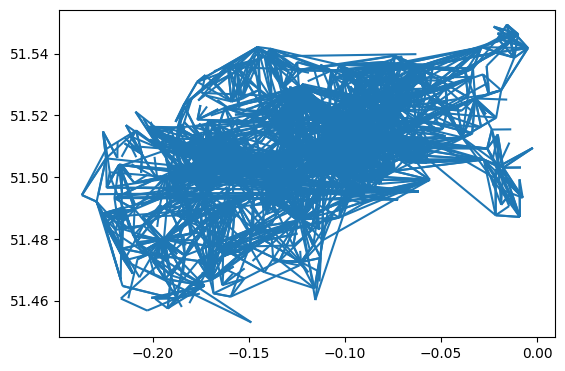
\includegraphics{labs/w05_interactive_files/figure-pdf/cell-32-output-1.png}

Plotting all lines is quite messy but we can use \texttt{folium} again
:) Unfortunately, we can't use \texttt{Choropleth} for
\texttt{LineString} geometries. We have to carry out some manual work.

\begin{Shaded}
\begin{Highlighting}[]
\ImportTok{import}\NormalTok{ json}
\ImportTok{import}\NormalTok{ jenkspy}
\ImportTok{import}\NormalTok{ matplotlib}
\ImportTok{import}\NormalTok{ matplotlib.pyplot }\ImportTok{as}\NormalTok{ plt}
\CommentTok{\# Convert the desire\_lines GeoDataFrame to GeoJSON}
\NormalTok{desire\_lines\_geojson }\OperatorTok{=}\NormalTok{ desire\_lines.to\_json()}

\CommentTok{\# breaks with fisher{-}jenks}
\NormalTok{breaks }\OperatorTok{=}\NormalTok{ jenkspy.jenks\_breaks(desire\_lines[}\StringTok{\textquotesingle{}journeys\textquotesingle{}}\NormalTok{], n\_classes}\OperatorTok{=}\DecValTok{5}\NormalTok{)}

\CommentTok{\# Use a Matplotlib colormap}
\NormalTok{cmap }\OperatorTok{=}\NormalTok{ plt.get\_cmap(}\StringTok{\textquotesingle{}Oranges\textquotesingle{}}\NormalTok{, }\BuiltInTok{len}\NormalTok{(breaks))  }\CommentTok{\# \textquotesingle{}viridis\textquotesingle{} can be replaced with any Matplotlib colormap}

\CommentTok{\# Generate colors for each break}
\NormalTok{colors }\OperatorTok{=}\NormalTok{ [matplotlib.colors.rgb2hex(cmap(i)) }\ControlFlowTok{for}\NormalTok{ i }\KeywordTok{in} \BuiltInTok{range}\NormalTok{(cmap.N)]}
\NormalTok{cmap}
\end{Highlighting}
\end{Shaded}


\includegraphics{labs/w05_interactive_files/figure-pdf/cell-33-output-1.png}

Let's define again a styling function for our lines.

\begin{Shaded}
\begin{Highlighting}[]
\CommentTok{\# Define the style function using the generated colors}
\KeywordTok{def}\NormalTok{ assign\_color(value):}
    \ControlFlowTok{for}\NormalTok{ i, break\_point }\KeywordTok{in} \BuiltInTok{enumerate}\NormalTok{(breaks[:}\OperatorTok{{-}}\DecValTok{1}\NormalTok{]):}
        \ControlFlowTok{if}\NormalTok{ value }\OperatorTok{\textless{}}\NormalTok{ breaks[i}\OperatorTok{+}\DecValTok{1}\NormalTok{]:}
            \ControlFlowTok{return}\NormalTok{ colors[i]}
    \ControlFlowTok{return}\NormalTok{ colors[}\OperatorTok{{-}}\DecValTok{1}\NormalTok{]}

\NormalTok{style\_function }\OperatorTok{=} \KeywordTok{lambda}\NormalTok{ feature: \{}
    \StringTok{\textquotesingle{}color\textquotesingle{}}\NormalTok{: assign\_color(feature[}\StringTok{\textquotesingle{}properties\textquotesingle{}}\NormalTok{][}\StringTok{\textquotesingle{}journeys\textquotesingle{}}\NormalTok{]),}
    \StringTok{\textquotesingle{}weight\textquotesingle{}}\NormalTok{: feature[}\StringTok{\textquotesingle{}properties\textquotesingle{}}\NormalTok{][}\StringTok{\textquotesingle{}share\_trips\textquotesingle{}}\NormalTok{]}\OperatorTok{*}\DecValTok{150}\NormalTok{,  }
    \StringTok{\textquotesingle{}opacity\textquotesingle{}}\NormalTok{: }\BuiltInTok{max}\NormalTok{(feature[}\StringTok{\textquotesingle{}properties\textquotesingle{}}\NormalTok{][}\StringTok{\textquotesingle{}share\_trips\textquotesingle{}}\NormalTok{]}\OperatorTok{*}\DecValTok{25}\NormalTok{, }\FloatTok{0.05}\NormalTok{)}
\NormalTok{\}}
\end{Highlighting}
\end{Shaded}

\begin{Shaded}
\begin{Highlighting}[]
\CommentTok{\# Create and display the Folium map}
\BuiltInTok{map} \OperatorTok{=}\NormalTok{ folium.Map(location}\OperatorTok{=}\NormalTok{[}\FloatTok{51.5074}\NormalTok{, }\OperatorTok{{-}}\FloatTok{0.1278}\NormalTok{], zoom\_start}\OperatorTok{=}\DecValTok{12}\NormalTok{, tiles}\OperatorTok{=}\StringTok{"CartoDB.DarkMatterNoLabels"}\NormalTok{)}
\NormalTok{folium.GeoJson(desire\_lines\_geojson, style\_function}\OperatorTok{=}\NormalTok{style\_function).add\_to(}\BuiltInTok{map}\NormalTok{)}
\BuiltInTok{map}
\end{Highlighting}
\end{Shaded}

\begin{verbatim}
<folium.folium.Map at 0x14882935e10>
\end{verbatim}

\textbf{Exercise}: Look at the documentation for one of the APIs that we
discussed last week (see the notebook of the practical session). - Think
of 2 ideas of web maps you could construct from your chosen API/data. -
Think about the basemap and data you would plot on top.

\emph{Folium} is just one of many packages that provide an easy way to
create interactive maps using data stored in (geo-)pandas
\texttt{DataFrames}. Other interesting libraries include:

\begin{itemize}
\tightlist
\item
  \href{https://geoviews.org/}{GeoViews}.
\item
  \href{https://docs.bokeh.org/en/latest/docs/gallery.html}{Bokeh}.
\item
  \href{https://docs.kepler.gl/docs/keplergl-jupyter}{kepler.gl}.
\item
  \href{https://deckgl.readthedocs.io/en/latest/}{pydeck}.
\end{itemize}

Neverthess, Folium allows for a huge degree of personalisation and it's
worth exploring further its
\href{https://python-visualization.github.io/folium/latest/reference.html}{documentation}.

\bookmarksetup{startatroot}

\chapter{Retrieving Data From
OpenStreetMap}\label{retrieving-data-from-openstreetmap}

\emph{Gabriele Filomena has readapted parts of this
\href{https://github.com/mszell/geospatialdatascience/blob/main/unit08_openstreetmap/lecture08.ipynb}{notebook}}
for preparing this notebook. Copyright (c) Michael Szell. Original
sources include:

\begin{itemize}
\tightlist
\item
  OSMnx examples: https://github.com/gboeing/osmnx-examples
\item
  pyrosm examples:
  https://pyrosm.readthedocs.io/en/latest/basics.html\#read-street-networks
\end{itemize}

The \textbf{Lecture slides} can be found
\href{https://github.com/GDSL-UL/wma/raw/main/html/w07.html}{here}.

\section{What is OpenStreetMap?}\label{what-is-openstreetmap}

OpenStreetMap is a free and open map service. It is a collaborative
global effort to collect free and open geodata. \emph{Source:
\href{https://wiki.openstreetmap.org/wiki/Logos}{wiki.openstreetmap.org}}.
OpenStreetMap (OSM) is a global collaborative (crowd-sourced) database
and project that aims at creating a free editable map of the world
containing of information about our environment. It contains data about
streets, buildings,different services, and landuse, to mention just a
few.

OSM has more than 8 million registered users who contribute around 4
million changes daily. Its database contains data that is described by
\href{http://wiki.openstreetmap.org/wiki/Stats}{more than 7 billion
nodes} (that make up lines, polygons and other objects). While the most
well-known side of OpenStreetMap is the map itself, the project is much
more than that. OSM's data can be used for many other purposes such as
\textbf{routing}, \textbf{geocoding}, \textbf{education}, and
\textbf{research}. OSM is also widely used for humanitarian response,
e.g., in crisis areas (e.g.~after natural disasters) and for fostering
economic development. Read more about humanitarian projects that use OSM
data from the \href{https://www.hotosm.org}{Humanitarian OpenStreetMap
Team (HOTOSM) website}.

\subsection{Main tools in this lesson}\label{main-tools-in-this-lesson}

\subsubsection{OSMnx}\label{osmnx}

This week we will explore a Python package called
\href{https://github.com/gboeing/osmnx}{\texttt{OSMnx}} that can be used
to retrieve street networks from OpenStreetMap, and construct, analyse,
and visualise them. \texttt{OSMnx} can also fetch most of the other data
stored in OSM, such as building footprints, transport networks, parks,
Points of Interest, etc..\texttt{OSMNx} also includes tools to find
routes on a network downloaded from OpenStreetMap, and implements
algorithms for finding shortest connections for walking, cycling, or
driving.

To get an overview of the capabilities of the package, please refer to
the following scientific article describing the package:

\begin{quote}
Boeing, G. 2017.
\href{https://www.researchgate.net/publication/309738462_OSMnx_New_Methods_for_Acquiring_Constructing_Analyzing_and_Visualizing_Complex_Street_Networks}{``OSMnx:
New Methods for Acquiring, Constructing, Analyzing, \textgreater{} and
Visualizing Complex Street \textgreater{} Networks.''} Computers,
Environment and Urban Systems 65, 126-139.
doi:10.1016/j.compenvurbsys.2017.05.004
\end{quote}

\subsubsection{NetworkX}\label{networkx}

We will also use
\href{https://networkx.github.io/documentation//}{\texttt{NetworkX}} to
manipulate and analyse the street network data retrieved from
OpenStreetMap. NetworkX is a Python package that can be used to create,
manipulate, and study the structure, dynamics, and functions of complex
networks. \texttt{OSMNx} is built on top \texttt{NetworkX} and
\texttt{GeoPandas}.

\begin{Shaded}
\begin{Highlighting}[]
\ImportTok{import}\NormalTok{ geopandas }\ImportTok{as}\NormalTok{ gpd}
\ImportTok{import}\NormalTok{ osmnx }\ImportTok{as}\NormalTok{ ox}
\ImportTok{import}\NormalTok{ numpy }\ImportTok{as}\NormalTok{ np}
\ImportTok{import}\NormalTok{ networkx }\ImportTok{as}\NormalTok{ nx}
\ImportTok{import}\NormalTok{ pandas }\ImportTok{as}\NormalTok{ pd}

\OperatorTok{\%}\NormalTok{matplotlib inline}
\end{Highlighting}
\end{Shaded}

\section{Download, manipulate, and visualise OpenStreetMap data with
OSMnx}\label{download-manipulate-and-visualise-openstreetmap-data-with-osmnx}

A useful feature of \texttt{OSMNx} is its easy-to-use tools to download
\href{http://www.openstreetmap.org}{OpenStreetMap} data via the
project's
\href{http://wiki.openstreetmap.org/wiki/Overpass_API}{OverPass API}. In
this section, we will learn how to download and visualise the street
network and additional data from OpenStreetMap covering different areas
of interest.

\subsection{Boundaries from
OpenStreetMap}\label{boundaries-from-openstreetmap}

\texttt{OSMnx} lets you download place boundary geometries from
OpenStreetMap, project them, and plot them. For a more in-depth
demonstration of querying by place, see
\href{03-graph-place-queries.ipynb}{this notebook}.

\textbf{Important}:

Data downloaded from OSM are always in the WGS crs. You need to convert
it for any type of spatial operation or computation to the appropriate
coordinate reference system.

\begin{Shaded}
\begin{Highlighting}[]
\CommentTok{\# get the boundary polygon for manhattan, project it, and plot it}
\NormalTok{city }\OperatorTok{=}\NormalTok{ ox.geocode\_to\_gdf(}\StringTok{"Manhattan"}\NormalTok{)}
\NormalTok{ax }\OperatorTok{=}\NormalTok{ city.plot(fc}\OperatorTok{=}\StringTok{"gray"}\NormalTok{, ec}\OperatorTok{=}\StringTok{"none"}\NormalTok{)}
\NormalTok{ax.axis(}\StringTok{"off"}\NormalTok{)}
\end{Highlighting}
\end{Shaded}

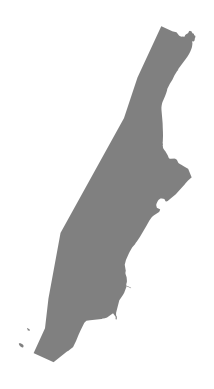
\includegraphics{labs/w07_OSM_files/figure-pdf/cell-3-output-1.png}

\begin{Shaded}
\begin{Highlighting}[]
\NormalTok{bulgaria }\OperatorTok{=}\NormalTok{ ox.geocode\_to\_gdf(}\StringTok{"Bulgaria"}\NormalTok{)}
\NormalTok{ax }\OperatorTok{=}\NormalTok{ bulgaria.plot(fc}\OperatorTok{=}\StringTok{"gray"}\NormalTok{, ec}\OperatorTok{=}\StringTok{"none"}\NormalTok{)}
\NormalTok{ax.axis(}\StringTok{"off"}\NormalTok{)}
\end{Highlighting}
\end{Shaded}

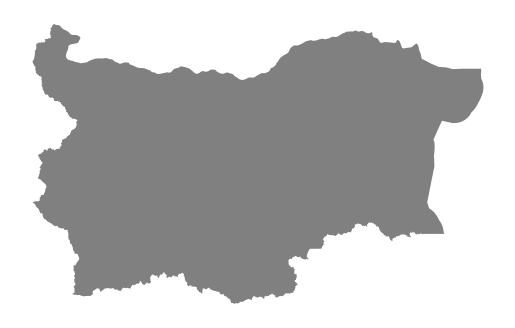
\includegraphics{labs/w07_OSM_files/figure-pdf/cell-4-output-1.png}

\begin{Shaded}
\begin{Highlighting}[]
\CommentTok{\# get boundary polygons for several authorities in the UK, and plot}
\NormalTok{place\_names }\OperatorTok{=}\NormalTok{ [}\StringTok{"Merseyside"}\NormalTok{, }\StringTok{"Greater Manchester"}\NormalTok{, }\StringTok{"Cheshire"}\NormalTok{]}
\NormalTok{places }\OperatorTok{=}\NormalTok{ ox.geocode\_to\_gdf(place\_names)}
\NormalTok{ax }\OperatorTok{=}\NormalTok{ places.plot(fc}\OperatorTok{=}\StringTok{"gray"}\NormalTok{, ec}\OperatorTok{=}\StringTok{"red"}\NormalTok{)}
\NormalTok{\_ }\OperatorTok{=}\NormalTok{ ax.axis(}\StringTok{"off"}\NormalTok{)}
\end{Highlighting}
\end{Shaded}

\includegraphics{labs/w07_OSM_files/figure-pdf/cell-5-output-1.png}

\subsection{Download and model Street
Networks}\label{download-and-model-street-networks}

The
\href{https://osmnx.readthedocs.io/en/stable/osmnx.html\#module-osmnx.graph}{\texttt{osmnx.graph}module}
downloads data to construct a routable road network graph, based on an
user-defined area of interest. This area of interest can be specified,
for instance, using a place name, a bounding box, or a polygon. In the
place name query, OSMnx uses the Nominatim Geocoding API. This means
that place names should exist in the OpenStreetMap database (run a test
search at \href{https://www.openstreetmap.org/}{openstreetmap.org} or
\href{https://nominatim.openstreetmap.org/ui/search.html}{nominatim.openstreetmap.org}).
\texttt{OSMnx}, amongst its several functionalities, lets you analyise,
plot, and export the network in different file formats. The downloaded
street networks are by default \textbf{directed} and preserve one-way
directionality. For a more in-depth demonstration of creating street
networks, see \href{03-graph-place-queries.ipynb}{this notebook}.

You can download a street network by providing OSMnx any of the
following (demonstrated in the examples below): - a bounding box - a
lat-long point plus a distance - an address plus a distance - a place
name or list of place names (to automatically geocode and get the
boundary of) - a polygon of the desired street network's boundaries - a
.osm formatted xml file

You can also specify several different network types: - \texttt{drive} -
get drivable public streets (but not service roads) -
\texttt{drive\_service} - get drivable streets, including service roads
- \texttt{walk} - get all streets and paths that pedestrians can use
(this network type ignores one-way directionality) - \texttt{bike} - get
all streets and paths that cyclists can use - \texttt{all} - download
all non-private OSM streets and paths (this is the default network type
unless you specify a different one) - \texttt{all\_private} - download
all OSM streets and paths, including private-access ones

\subsubsection{Method \#1: Passing a bounding
box}\label{method-1-passing-a-bounding-box}

This constructs the network from all the OSM nodes and ways within the
bounding box. The plot function is built on \texttt{Matplotlib}, thus it
follows the procedures and methods discussed in session II.

\begin{Shaded}
\begin{Highlighting}[]
\CommentTok{\# define a bounding box in San Francisco}
\NormalTok{north, south, east, west }\OperatorTok{=} \FloatTok{37.79}\NormalTok{, }\FloatTok{37.78}\NormalTok{, }\OperatorTok{{-}}\FloatTok{122.41}\NormalTok{, }\OperatorTok{{-}}\FloatTok{122.43}
\CommentTok{\# define a bounding box around ITU}
\NormalTok{north, south, east, west }\OperatorTok{=} \FloatTok{55.6646}\NormalTok{, }\FloatTok{55.6540}\NormalTok{, }\FloatTok{12.5767}\NormalTok{, }\FloatTok{12.6077}

\CommentTok{\# create network from that bounding box}
\NormalTok{G }\OperatorTok{=}\NormalTok{ ox.graph\_from\_bbox(north, south, east, west, network\_type}\OperatorTok{=}\StringTok{"drive\_service"}\NormalTok{)}
\NormalTok{ox.plot\_graph(G, node\_color}\OperatorTok{=}\StringTok{"r"}\NormalTok{, figsize}\OperatorTok{=}\NormalTok{(}\DecValTok{8}\NormalTok{, }\DecValTok{8}\NormalTok{))}
\end{Highlighting}
\end{Shaded}

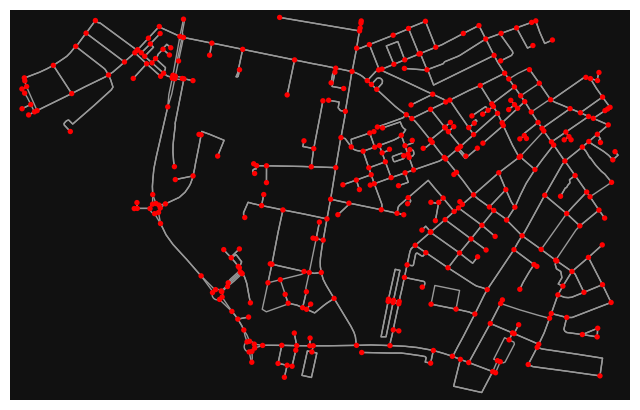
\includegraphics{labs/w07_OSM_files/figure-pdf/cell-6-output-1.png}

\subsubsection{Method \#2: Passing a lat-lng point and bounding box
distance in
meters}\label{method-2-passing-a-lat-lng-point-and-bounding-box-distance-in-meters}

This creates a bounding box \emph{n} meters North, South, East, and West
of the point, then constructs the network from all the OSM nodes and
ways within the bounding box. \href{https://bboxfinder.com}{Here's a
useful tool for defining bboxes}

\begin{Shaded}
\begin{Highlighting}[]
\CommentTok{\# define a point at the corner of California St and Mason St in SF}
\NormalTok{location\_point }\OperatorTok{=}\NormalTok{ (}\FloatTok{37.791427}\NormalTok{, }\OperatorTok{{-}}\FloatTok{122.410018}\NormalTok{)}
\CommentTok{\# create bikeable network from point, inside bounding box of N, S, E, W each 750m from point}
\NormalTok{G }\OperatorTok{=}\NormalTok{ ox.graph\_from\_point(location\_point, dist}\OperatorTok{=}\DecValTok{750}\NormalTok{, dist\_type}\OperatorTok{=}\StringTok{"bbox"}\NormalTok{, network\_type}\OperatorTok{=}\StringTok{"bike"}\NormalTok{)}
\NormalTok{ox.plot\_graph(G, node\_color}\OperatorTok{=}\StringTok{"r"}\NormalTok{, figsize}\OperatorTok{=}\NormalTok{(}\DecValTok{5}\NormalTok{,}\DecValTok{5}\NormalTok{))}
\end{Highlighting}
\end{Shaded}

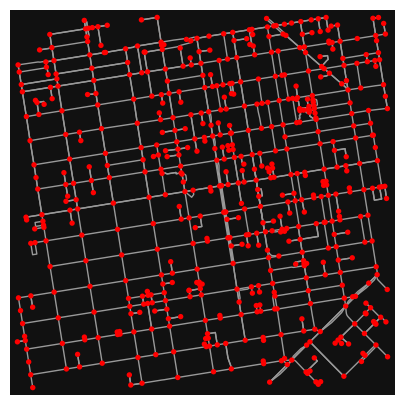
\includegraphics{labs/w07_OSM_files/figure-pdf/cell-7-output-1.png}

\subsubsection{\texorpdfstring{Method \#3: Passing a lat-lng point and
\emph{network} distance in
meters}{Method \#3: Passing a lat-lng point and network distance in meters}}\label{method-3-passing-a-lat-lng-point-and-network-distance-in-meters}

This creates a bounding box \emph{n} meters North, South, East, and West
of the point, then constructs the network from all the OSM nodes and
ways within the bounding box. Then it truncates the network by removing
all nodes further than \emph{n} meters from the point along the network.

\begin{Shaded}
\begin{Highlighting}[]
\NormalTok{location\_point }\OperatorTok{=}\NormalTok{ (}\FloatTok{53.40}\NormalTok{, }\OperatorTok{{-}}\FloatTok{2.99}\NormalTok{)}
\CommentTok{\# create network only of nodes within 750m along the network from point}
\NormalTok{G1 }\OperatorTok{=}\NormalTok{ ox.graph\_from\_point(location\_point, dist}\OperatorTok{=}\DecValTok{1000}\NormalTok{, dist\_type}\OperatorTok{=}\StringTok{"network"}\NormalTok{)}
\NormalTok{ox.plot\_graph(G1, node\_color}\OperatorTok{=}\StringTok{"none"}\NormalTok{, figsize}\OperatorTok{=}\NormalTok{(}\DecValTok{5}\NormalTok{,}\DecValTok{5}\NormalTok{))}
\end{Highlighting}
\end{Shaded}

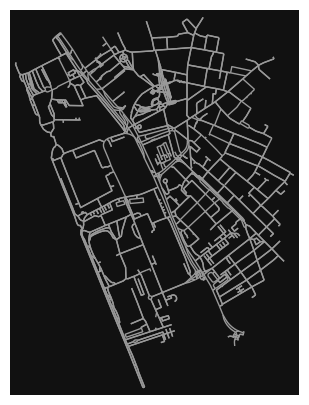
\includegraphics{labs/w07_OSM_files/figure-pdf/cell-8-output-1.png}

\emph{Note} the plot above shows the network within 750m (traveling
distance along the network) from the \texttt{location\_point}. By
default, the \texttt{network\_type} parameter value is \texttt{all},
meaning that we do not filter out paths that restrict certain types of
traffic. This also means that one-way streets are honored as one-way and
you cannot travel the wrong direction down them. Thus, the 750m takes
into account only those nodes you can reach within 500m while only
traveling in the allowed direction of the street. Instead (below), we
can specify
\texttt{network\_type=\textquotesingle{}walk\textquotesingle{}} to build
a street network only of paths that walking is allowed on. This also
makes every path bi-directional in the directed network, because you can
walk in either direction on the sidewalk of a one-way street. Thus, the
750m now takes into account those nodes you can reach within 750m while
traveling in either direction (even if it's a one-way street).

\begin{Shaded}
\begin{Highlighting}[]
\CommentTok{\# create network only of nodes within 750m walking along the network from point, only walkable edges}
\NormalTok{G2 }\OperatorTok{=}\NormalTok{ ox.graph\_from\_point(location\_point, dist}\OperatorTok{=}\DecValTok{750}\NormalTok{, dist\_type}\OperatorTok{=}\StringTok{"network"}\NormalTok{, network\_type}\OperatorTok{=}\StringTok{"walk"}\NormalTok{)}
\NormalTok{ox.plot\_graph(G2, node\_color}\OperatorTok{=}\StringTok{"none"}\NormalTok{, figsize}\OperatorTok{=}\NormalTok{(}\DecValTok{5}\NormalTok{,}\DecValTok{5}\NormalTok{))}
\end{Highlighting}
\end{Shaded}

\includegraphics{labs/w07_OSM_files/figure-pdf/cell-9-output-1.png}

\subsubsection{\texorpdfstring{Method \#4, Passing an address and
distance (\emph{bounding box} or \emph{network}) in
meters}{Method \#4, Passing an address and distance (bounding box or network) in meters}}\label{method-4-passing-an-address-and-distance-bounding-box-or-network-in-meters}

This geocodes the address, creates a bounding box, downloads the
network, then truncates it by network distance (if
distance\_type=`network').

\begin{Shaded}
\begin{Highlighting}[]
\CommentTok{\# network from address, including only nodes within 1km along the network from the address}
\NormalTok{G }\OperatorTok{=}\NormalTok{ ox.graph\_from\_address(address}\OperatorTok{=}\StringTok{"350 5th Ave, New York, NY"}\NormalTok{, dist}\OperatorTok{=}\DecValTok{1000}\NormalTok{, dist\_type}\OperatorTok{=}\StringTok{"network"}\NormalTok{, network\_type}\OperatorTok{=}\StringTok{"drive"}\NormalTok{)}
\NormalTok{ox.plot\_graph(G, node\_color}\OperatorTok{=}\StringTok{"r"}\NormalTok{, figsize}\OperatorTok{=}\NormalTok{(}\DecValTok{5}\NormalTok{,}\DecValTok{5}\NormalTok{))}
\end{Highlighting}
\end{Shaded}

\includegraphics{labs/w07_OSM_files/figure-pdf/cell-10-output-1.png}

\subsubsection{Method \#5: Passing a place
name}\label{method-5-passing-a-place-name}

This geocodes the place name, gets the place's boundary shape polygon
and bounding box, downloads the network within the bounding box, then
truncates it to the place's boundary polygon.

\begin{Shaded}
\begin{Highlighting}[]
\NormalTok{G }\OperatorTok{=}\NormalTok{ ox.graph\_from\_place(}\StringTok{"Bastia, Corsica"}\NormalTok{, network\_type}\OperatorTok{=}\StringTok{"drive"}\NormalTok{)}
\NormalTok{ox.plot\_graph(G, node\_color}\OperatorTok{=}\StringTok{"none"}\NormalTok{) }\CommentTok{\# without plotting nodes}
\end{Highlighting}
\end{Shaded}

\includegraphics{labs/w07_OSM_files/figure-pdf/cell-11-output-1.png}

Be aware that this is a \texttt{MultiDiGraph}, i.e.~a multigraph
(parallel edges are possible) that is directed. Because there can be
multiple links between a pair of nodes, each link is identified with a
triple: (node1id, node2id, counter)

\begin{Shaded}
\begin{Highlighting}[]
\BuiltInTok{list}\NormalTok{(G.edges)[:}\DecValTok{10}\NormalTok{]}
\end{Highlighting}
\end{Shaded}

\begin{verbatim}
[(60370565, 338870652, 0),
 (60370565, 338870615, 0),
 (60370586, 338870618, 0),
 (60370599, 338870618, 0),
 (60370599, 60370602, 0),
 (60370602, 60370612, 0),
 (60370602, 60370599, 0),
 (60370612, 721266231, 0),
 (60370612, 60370602, 0),
 (60370622, 2358639572, 0)]
\end{verbatim}

These values above correspond to \texttt{u}, \texttt{v} and
\texttt{key}. More on that later, but, essentially, \texttt{u} is the id
of the ``from-node'' and \texttt{v} the id of the ``to-node''

\subsubsection{Method \#6 Passing a Poylgon in the WGS
crs}\label{method-6-passing-a-poylgon-in-the-wgs-crs}

\begin{Shaded}
\begin{Highlighting}[]
\CommentTok{\# get the boundary polygon for Sarajevo, and plot it}
\NormalTok{city }\OperatorTok{=}\NormalTok{ ox.geocode\_to\_gdf(}\StringTok{"Sarajevo, Bosnia"}\NormalTok{)}
\NormalTok{city\_proj }\OperatorTok{=}\NormalTok{ ox.project\_gdf(city)}
\NormalTok{ax }\OperatorTok{=}\NormalTok{ city\_proj.plot(fc}\OperatorTok{=}\StringTok{"gray"}\NormalTok{, ec}\OperatorTok{=}\StringTok{"none"}\NormalTok{)}
\NormalTok{ax.axis(}\StringTok{"off"}\NormalTok{)}\OperatorTok{;}
\end{Highlighting}
\end{Shaded}

\includegraphics{labs/w07_OSM_files/figure-pdf/cell-13-output-1.png}

\begin{Shaded}
\begin{Highlighting}[]
\NormalTok{sarajevo }\OperatorTok{=}\NormalTok{ ox.geocode\_to\_gdf(}\StringTok{"Sarajevo, Bosnia"}\NormalTok{)}
\NormalTok{polygon }\OperatorTok{=}\NormalTok{ sarajevo[}\StringTok{"geometry"}\NormalTok{].iloc[}\DecValTok{0}\NormalTok{]}

\NormalTok{G }\OperatorTok{=}\NormalTok{ ox.graph\_from\_polygon(polygon, network\_type}\OperatorTok{=}\StringTok{"drive\_service"}\NormalTok{)}
\NormalTok{ox.plot\_graph(G, node\_size}\OperatorTok{=}\DecValTok{0}\NormalTok{, edge\_color}\OperatorTok{=}\StringTok{"w"}\NormalTok{, edge\_linewidth}\OperatorTok{=}\FloatTok{0.3}\NormalTok{)}\OperatorTok{;}
\end{Highlighting}
\end{Shaded}

\includegraphics{labs/w07_OSM_files/figure-pdf/cell-14-output-1.png}

\subsection{Simplifying and Cleaning the Street Network
Topology}\label{simplifying-and-cleaning-the-street-network-topology}

Simplification is normally done by \texttt{OSMnx} automatically under
the hood, but we can break it out to see how it works. OpenStreetMap
nodes are weird. They include intersections, but they also include all
the points along a single block where the street curves. The latter are
not nodes in the graph theory sense, so we remove them algorithmically
and consolidate the set of edges between ``true'' network nodes into a
single edge. There are two simplification modes, strict and non-strict.
The main difference is that unlike strict mode, non-strict mode allows
simplification to an ``expansion graph'' (i.e., if the graph were
undirected, nodes with degree 2 as long as the incident edges have
different OSM IDs).

\begin{Shaded}
\begin{Highlighting}[]
\CommentTok{\# create a network around some (lat, lng) point but do not simplify it yet}
\NormalTok{location\_point }\OperatorTok{=}\NormalTok{ (}\FloatTok{33.299896}\NormalTok{, }\OperatorTok{{-}}\FloatTok{111.831638}\NormalTok{)}
\NormalTok{G }\OperatorTok{=}\NormalTok{ ox.graph\_from\_point(location\_point, network\_type}\OperatorTok{=}\StringTok{"drive\_service"}\NormalTok{, dist}\OperatorTok{=}\DecValTok{500}\NormalTok{, simplify}\OperatorTok{=}\VariableTok{False}\NormalTok{)}
\NormalTok{ox.plot\_graph(G, node\_color}\OperatorTok{=}\StringTok{"r"}\NormalTok{, figsize}\OperatorTok{=}\NormalTok{(}\DecValTok{5}\NormalTok{,}\DecValTok{5}\NormalTok{))}
\end{Highlighting}
\end{Shaded}

\includegraphics{labs/w07_OSM_files/figure-pdf/cell-15-output-1.png}

\begin{Shaded}
\begin{Highlighting}[]
\CommentTok{\# turn off strict mode and see what nodes we\textquotesingle{}d remove, in yellow}
\NormalTok{colors }\OperatorTok{=}\NormalTok{ [}\StringTok{"r"} \ControlFlowTok{if}\NormalTok{ ox.simplification.\_is\_endpoint(G, node) }\ControlFlowTok{else} \StringTok{"y"} \ControlFlowTok{for}\NormalTok{ node }\KeywordTok{in}\NormalTok{ G.nodes()]}
\NormalTok{fig, ax }\OperatorTok{=}\NormalTok{ ox.plot\_graph(G, node\_color}\OperatorTok{=}\NormalTok{colors, figsize}\OperatorTok{=}\NormalTok{(}\DecValTok{5}\NormalTok{,}\DecValTok{5}\NormalTok{))}
\end{Highlighting}
\end{Shaded}

\includegraphics{labs/w07_OSM_files/figure-pdf/cell-16-output-1.png}

The yellow markers above are OSM nodes. We'll remove the nodes in yellow
as they're not real network nodes (intersections/dead-ends).

\begin{Shaded}
\begin{Highlighting}[]
\CommentTok{\# simplify the network}
\NormalTok{G }\OperatorTok{=}\NormalTok{ ox.simplify\_graph(G)}
\NormalTok{ox.plot\_graph(G, node\_color}\OperatorTok{=}\StringTok{"r"}\NormalTok{, figsize}\OperatorTok{=}\NormalTok{(}\DecValTok{5}\NormalTok{,}\DecValTok{5}\NormalTok{))}
\end{Highlighting}
\end{Shaded}

\includegraphics{labs/w07_OSM_files/figure-pdf/cell-17-output-1.png}

\subsubsection{Optional: Complex intersection
consolidation}\label{optional-complex-intersection-consolidation}

Many real-world street networks feature complex intersections and
traffic circles, resulting in a cluster of graph nodes where there is
really just one true intersection. Similarly, divided roads are often
represented by separate centerline edges: the intersection of two
divided roads thus creates 4 nodes, representing where each edge
intersects a perpendicular edge, but these 4 nodes represent a single
intersection in the real world. Traffic circles similarly create a
cluster of nodes where each street's edge intersects the roundabout.

\texttt{OSMnx} can consolidate nearby intersections and optionally
rebuild the graph's topology.

\begin{Shaded}
\begin{Highlighting}[]
\CommentTok{\# get a street network and plot it with all edge intersections}
\NormalTok{point }\OperatorTok{=} \FloatTok{55.667708}\NormalTok{, }\FloatTok{12.596266}
\NormalTok{G }\OperatorTok{=}\NormalTok{ ox.graph\_from\_point(point, network\_type}\OperatorTok{=}\StringTok{"drive"}\NormalTok{, dist}\OperatorTok{=}\DecValTok{500}\NormalTok{)}
\NormalTok{ox.plot\_graph(G, node\_color}\OperatorTok{=}\StringTok{"r"}\NormalTok{, figsize}\OperatorTok{=}\NormalTok{(}\DecValTok{5}\NormalTok{,}\DecValTok{5}\NormalTok{))}
\end{Highlighting}
\end{Shaded}

\includegraphics{labs/w07_OSM_files/figure-pdf/cell-18-output-1.png}

Notice the complex intersections creating clusters of nodes.

We'll specify that any nodes with 15 meter buffers of each other in this
network are part of the same intersection. Adjust this tolerance based
on the street design standards in the community you are examining, and
use a projected graph to work in meaningful units like meters. We'll
also specify that we do not want dead-ends returned in our list of
consolidated intersections.

\begin{Shaded}
\begin{Highlighting}[]
\CommentTok{\# get a GeoSeries of consolidated intersections}
\NormalTok{G\_proj }\OperatorTok{=}\NormalTok{ ox.project\_graph(G)}
\NormalTok{intersections }\OperatorTok{=}\NormalTok{ ox.consolidate\_intersections(G\_proj, rebuild\_graph}\OperatorTok{=}\VariableTok{False}\NormalTok{, tolerance}\OperatorTok{=}\DecValTok{15}\NormalTok{, dead\_ends}\OperatorTok{=}\VariableTok{False}\NormalTok{)}
\CommentTok{\# compare to number of nodes in original graph}
\BuiltInTok{print}\NormalTok{(}\BuiltInTok{len}\NormalTok{(intersections), }\StringTok{"vs"}\NormalTok{, }\BuiltInTok{len}\NormalTok{(G))}
\end{Highlighting}
\end{Shaded}

\begin{verbatim}
73 vs 122
\end{verbatim}

Note that these cleaned up intersections give us more accurate
intersection counts and densities, but do not alter or integrate with
the network's topology. To do that, we need to \textbf{rebuild the
graph}.

\begin{Shaded}
\begin{Highlighting}[]
\CommentTok{\# consolidate intersections and rebuild graph topology}
\CommentTok{\# this reconnects edge geometries to the new consolidated nodes}
\NormalTok{cleaned }\OperatorTok{=}\NormalTok{ ox.consolidate\_intersections(G\_proj, rebuild\_graph}\OperatorTok{=}\VariableTok{True}\NormalTok{, tolerance}\OperatorTok{=}\DecValTok{15}\NormalTok{, dead\_ends}\OperatorTok{=}\VariableTok{False}\NormalTok{)}
\NormalTok{ox.plot\_graph(cleaned, node\_color}\OperatorTok{=}\StringTok{"r"}\NormalTok{, figsize}\OperatorTok{=}\NormalTok{(}\DecValTok{5}\NormalTok{,}\DecValTok{5}\NormalTok{))}
\end{Highlighting}
\end{Shaded}

\includegraphics{labs/w07_OSM_files/figure-pdf/cell-20-output-1.png}

Notice how many nodes are merged into a new single centroid node, with
edge geometries extended to connect to it. Similar consolidation occurs
at the intersection of the divided roads.

\textbf{Note}

Running \texttt{consolidate\_intersections} with
\texttt{rebuild\_graph=True} may yield somewhat (but not very) different
intersection counts/densities compared to \texttt{rebuild\_graph=False}.
The difference lies in that the latter just merges buffered node points
that overlap, whereas the former checks the topology of the overlapping
node buffers before merging them. This prevents topologically remote but
spatially proximate nodes from being merged. For example: - A street
intersection may lie directly below a freeway overpass's intersection
with an on-ramp. We would not want to merge these together and connnect
their edges: they are distinct junctions in the system of roads. - In a
residential neighborhood, a bollarded street may create a dead-end
immediately next to an intersection or traffic circle. We would not want
to merge this dead-end with the intersection and connect their edges.

These examples illustrate (two-dimensional) geometric proximity, but
topological remoteness. Accordingly, in some situations we may expect
higher intersection counts when using \texttt{rebuild\_graph=True}
because it is more cautious with merging in these cases. The trade-off
is that it has higher time complexity than
\texttt{rebuild\_graph=False}.

\subsection{From OSMNX to NetworkX and Geopandas
Classes}\label{from-osmnx-to-networkx-and-geopandas-classes}

Now, we have seen how to use some basic \texttt{osmnx} functions to
obtain a graph representation of the street network. While this is
simple and strightforward, I advise working on the street network
represented as \texttt{geopandas.GeoDataFrame}s and \texttt{networkx}
graphs. While at the beginning this may be more tedious, it also gives
us much more control, both in terms of visualisation anad analysis
depth. Before proceeding, it is important to keep in mind what type of
graphs can be modelled through OSMNx and NetworkX, and what that means
for the infrastructure we are modelling.

Have a look at NetworkX
\href{https://networkx.org/documentation/stable/reference/classes/index.html}{documentation}
for details.

\textbf{By default, the graphs obtained through OSMNX are
`MultiDiGraph'}

\begin{Shaded}
\begin{Highlighting}[]
\NormalTok{siracusa\_graph }\OperatorTok{=}\NormalTok{ ox.graph\_from\_address(}\StringTok{"Largo XXV Luglio, Siracusa"}\NormalTok{, network\_type}\OperatorTok{=}\StringTok{"all"}\NormalTok{, dist }\OperatorTok{=} \DecValTok{2500}\NormalTok{)}
\NormalTok{sicily\_epsg }\OperatorTok{=} \StringTok{\textquotesingle{}EPSG:23030\textquotesingle{}}
\NormalTok{nodes }\OperatorTok{=}\NormalTok{ ox.graph\_to\_gdfs(siracusa\_graph, nodes}\OperatorTok{=}\VariableTok{True}\NormalTok{, node\_geometry}\OperatorTok{=}\VariableTok{True}\NormalTok{, edges }\OperatorTok{=} \VariableTok{False}\NormalTok{).to\_crs(crs }\OperatorTok{=} \DecValTok{23030}\NormalTok{)}
\NormalTok{edges }\OperatorTok{=}\NormalTok{ ox.graph\_to\_gdfs(siracusa\_graph, nodes}\OperatorTok{=}\VariableTok{False}\NormalTok{, edges }\OperatorTok{=}  \VariableTok{True}\NormalTok{, fill\_edge\_geometry}\OperatorTok{=}\VariableTok{True}\NormalTok{).to\_crs(crs }\OperatorTok{=} \DecValTok{23030}\NormalTok{)}
\end{Highlighting}
\end{Shaded}

\begin{Shaded}
\begin{Highlighting}[]
\NormalTok{edges.plot(lw }\OperatorTok{=} \FloatTok{0.2}\NormalTok{, color }\OperatorTok{=} \StringTok{\textquotesingle{}red\textquotesingle{}}\NormalTok{)}
\end{Highlighting}
\end{Shaded}

\includegraphics{labs/w07_OSM_files/figure-pdf/cell-22-output-1.png}

We can visualise major roads on top of the stree network:

\begin{Shaded}
\begin{Highlighting}[]
\NormalTok{ax }\OperatorTok{=}\NormalTok{ edges[edges.highway.isin([}\StringTok{\textquotesingle{}primary\textquotesingle{}}\NormalTok{, }\StringTok{\textquotesingle{}secondary\textquotesingle{}}\NormalTok{])].plot()}
\NormalTok{edges.plot(ax }\OperatorTok{=}\NormalTok{ ax, lw }\OperatorTok{=} \FloatTok{0.2}\NormalTok{, color }\OperatorTok{=} \StringTok{\textquotesingle{}red\textquotesingle{}}\NormalTok{)}
\end{Highlighting}
\end{Shaded}

\includegraphics{labs/w07_OSM_files/figure-pdf/cell-23-output-1.png}

\begin{Shaded}
\begin{Highlighting}[]
\NormalTok{edges.head()}
\end{Highlighting}
\end{Shaded}

\begin{longtable}[]{@{}lllllllllllllllllll@{}}
\toprule\noalign{}
& & & osmid & highway & maxspeed & oneway & reversed & length & geometry
& name & lanes & junction & ref & bridge & access & service & tunnel &
width \\
u & v & key & & & & & & & & & & & & & & & & \\
\midrule\noalign{}
\endhead
\bottomrule\noalign{}
\endlastfoot
\multirow{3}{=}{33566408} & 297074052 & 0 & 828152472 & secondary & 50 &
False & False & 63.755 & LINESTRING (2132529.446 4262765.911,
2132466.8... & NaN & NaN & NaN & NaN & NaN & NaN & NaN & NaN & NaN \\
& 9130394527 & 0 & 5028297 & residential & 50 & True & False & 46.925 &
LINESTRING (2132529.446 4262765.911, 2132535.5... & NaN & NaN & NaN &
NaN & NaN & NaN & NaN & NaN & NaN \\
& 7876226633 & 0 & {[}828152472, 836932525{]} & secondary & 50 & False &
True & 26.804 & LINESTRING (2132529.446 4262765.911, 2132538.7... & Via
Francesco Crispi & NaN & NaN & NaN & NaN & NaN & NaN & NaN & NaN \\
\multirow{2}{=}{33566411} & 8185067296 & 0 & 881159784 & secondary & 50
& True & False & 3.544 & LINESTRING (2133165.090 4262581.928,
2133165.4... & NaN & 2 & NaN & NaN & NaN & NaN & NaN & NaN & NaN \\
& 33566412 & 0 & 28114161 & residential & NaN & True & False & 62.841 &
LINESTRING (2133165.090 4262581.928, 2133163.3... & Via Nino Bixio & NaN
& NaN & NaN & NaN & NaN & NaN & NaN & NaN \\
\end{longtable}

\begin{Shaded}
\begin{Highlighting}[]
\NormalTok{nodes.head()}
\end{Highlighting}
\end{Shaded}

\begin{longtable}[]{@{}llllll@{}}
\toprule\noalign{}
& y & x & street\_count & highway & geometry \\
osmid & & & & & \\
\midrule\noalign{}
\endhead
\bottomrule\noalign{}
\endlastfoot
33566408 & 37.068451 & 15.280819 & 3 & NaN & POINT (2132529.446
4262765.911) \\
33566411 & 37.065793 & 15.287216 & 4 & NaN & POINT (2133165.090
4262581.928) \\
33566412 & 37.065258 & 15.286985 & 3 & NaN & POINT (2133156.199
4262517.746) \\
33566413 & 37.064692 & 15.286909 & 3 & NaN & POINT (2133162.078
4262452.755) \\
33566854 & 37.060586 & 15.293191 & 3 & NaN & POINT (2133819.897
4262104.005) \\
\end{longtable}

As you can see an edge's index is a \texttt{MultiIndex} given by
\texttt{u}, \texttt{v}, and \texttt{key}. \texttt{u} and \texttt{v} in
\texttt{networkx} language stand for ``from-node'' and ``to-node''.
\texttt{key}, on the other hand, indicates whether more than one edge
links \texttt{u} and \texttt{v}. When a pair of \texttt{u} and
\texttt{v} nodes have more then one edge, every other edge will have an
incrimental \texttt{key} value (the second one 1, the third one 2, etc.,
very rare that there are more than two edges per pair of nodes). This
means that we are dealing with a \texttt{MultiGraph} representation of
the street network. In other words, we have two street segments
connecting the same two nodes in different directions. This could, for
example, indicate that the directionality is accounted for (one-way
segments). Based on our objective and analysis, such an aspect might be
relevant, or not.

\subsubsection{\texorpdfstring{(Re)converting to a
\texttt{MultiGraph}/\texttt{MultiDiGraph}}{(Re)converting to a MultiGraph/MultiDiGraph}}\label{reconverting-to-a-multigraphmultidigraph}

First, we get rid of the \texttt{pandas} \texttt{MultiIndex} and we
verify whether we are working with bidirectional edges.

\begin{Shaded}
\begin{Highlighting}[]
\NormalTok{edges.reset\_index(inplace }\OperatorTok{=} \VariableTok{True}\NormalTok{)}
\NormalTok{edges[}\StringTok{\textquotesingle{}key\textquotesingle{}}\NormalTok{].}\BuiltInTok{sum}\NormalTok{()}
\end{Highlighting}
\end{Shaded}

\begin{verbatim}
95
\end{verbatim}

\begin{Shaded}
\begin{Highlighting}[]
\ImportTok{import}\NormalTok{ networkx }\ImportTok{as}\NormalTok{ nx}
\NormalTok{Mg }\OperatorTok{=}\NormalTok{ nx.MultiGraph()   }
\NormalTok{Mg.add\_nodes\_from(nodes.index)}
\end{Highlighting}
\end{Shaded}

Copying the nodes' attributes (this step is not particularly essential
unless we need some information associated with the nodes that we want
to use when executing \texttt{networkx} methods). Anything else we can
rely on the informaiton that is in the \texttt{GeoDataFrame}.

\begin{Shaded}
\begin{Highlighting}[]
\CommentTok{\# add the nodes\textquotesingle{} attributes}
\NormalTok{attributes }\OperatorTok{=}\NormalTok{ nodes.to\_dict()}

\ControlFlowTok{for}\NormalTok{ attribute\_name }\KeywordTok{in}\NormalTok{ nodes.columns:}
    \ControlFlowTok{if}\NormalTok{ nodes[attribute\_name].}\BuiltInTok{apply}\NormalTok{(}\KeywordTok{lambda}\NormalTok{ x: }\BuiltInTok{type}\NormalTok{(x) }\OperatorTok{==} \BuiltInTok{list}\NormalTok{).}\BuiltInTok{any}\NormalTok{(): }
        \ControlFlowTok{continue} 
    \CommentTok{\# only add this attribute to nodes which have a non{-}null value for it}
\NormalTok{    attribute\_values }\OperatorTok{=}\NormalTok{ \{k:v }\ControlFlowTok{for}\NormalTok{ k, v }\KeywordTok{in}\NormalTok{ attributes[attribute\_name].items() }\ControlFlowTok{if}\NormalTok{ pd.notnull(v)\}}
\NormalTok{    nx.set\_node\_attributes(Mg, name}\OperatorTok{=}\NormalTok{attribute\_name, values}\OperatorTok{=}\NormalTok{attribute\_values)}
\end{Highlighting}
\end{Shaded}

We do something similar for edges. In this case, it is more likely that
there is information that we want to copy, e.g.~the length of the edges,
into the \texttt{MultiGraph}.

\begin{Shaded}
\begin{Highlighting}[]
\NormalTok{edges[}\StringTok{\textquotesingle{}length\textquotesingle{}}\NormalTok{] }\OperatorTok{=}\NormalTok{ edges.geometry.length}

\CommentTok{\# add the edges and attributes that are not u, v, key, null, or of type list}
\CommentTok{\#\# u, v, and key are added directly as you can see from the last line}
\ControlFlowTok{for}\NormalTok{ row }\KeywordTok{in}\NormalTok{ edges.itertuples():}
\NormalTok{    attrs }\OperatorTok{=}\NormalTok{ \{label: value }\ControlFlowTok{for}\NormalTok{ label, value }\KeywordTok{in}\NormalTok{ row.\_asdict().items() }\ControlFlowTok{if}\NormalTok{ (label }\KeywordTok{not} \KeywordTok{in}\NormalTok{ [}\StringTok{\textquotesingle{}u\textquotesingle{}}\NormalTok{, }\StringTok{\textquotesingle{}v\textquotesingle{}}\NormalTok{, }\StringTok{\textquotesingle{}key\textquotesingle{}}\NormalTok{]) }\KeywordTok{and} 
\NormalTok{             (}\BuiltInTok{isinstance}\NormalTok{(value, }\BuiltInTok{list}\NormalTok{) }\KeywordTok{or}\NormalTok{ pd.notnull(value))\}}
\NormalTok{    Mg.add\_edge(row.u, row.v, key}\OperatorTok{=}\NormalTok{row.key, }\OperatorTok{**}\NormalTok{attrs)}
\end{Highlighting}
\end{Shaded}

\subsubsection{\texorpdfstring{Converting to a
\texttt{Graph}/\texttt{DiGraph}}{Converting to a Graph/DiGraph}}\label{converting-to-a-graphdigraph}

In this case, we need to get rid of the ``duplicated'' edges. For the
sake of simplicity, we remove al the edges with \texttt{key} equal to 1.
This is a very rough approach.

\begin{Shaded}
\begin{Highlighting}[]
\NormalTok{edges\_copy }\OperatorTok{=}\NormalTok{ edges[edges.key }\OperatorTok{==} \DecValTok{0}\NormalTok{].copy()}
\NormalTok{G }\OperatorTok{=}\NormalTok{ nx.Graph()   }
\NormalTok{G.add\_nodes\_from(nodes.index)}
\end{Highlighting}
\end{Shaded}

Then, we copy the attributes with the same approach used before,
although, this time, withouth adding the \texttt{key} value to the
edges. The function \texttt{add\_edge}of the class the \texttt{graph}
does not take the \texttt{key} argument as there could be only one edge
between two nodes.

\begin{Shaded}
\begin{Highlighting}[]
\CommentTok{\# ignore fields containing values of type list}
\NormalTok{attributes }\OperatorTok{=}\NormalTok{ nodes.to\_dict()}

\ControlFlowTok{for}\NormalTok{ attribute\_name }\KeywordTok{in}\NormalTok{ nodes.columns:}
    \ControlFlowTok{if}\NormalTok{ nodes[attribute\_name].}\BuiltInTok{apply}\NormalTok{(}\KeywordTok{lambda}\NormalTok{ x: }\BuiltInTok{type}\NormalTok{(x) }\OperatorTok{==} \BuiltInTok{list}\NormalTok{).}\BuiltInTok{any}\NormalTok{(): }
        \ControlFlowTok{continue}    
    \CommentTok{\# only add this attribute to nodes which have a non{-}null value for it}
\NormalTok{    attribute\_values }\OperatorTok{=}\NormalTok{ \{k: v }\ControlFlowTok{for}\NormalTok{ k, v }\KeywordTok{in}\NormalTok{ attributes[attribute\_name].items() }\ControlFlowTok{if}\NormalTok{ pd.notnull(v)\}}
\NormalTok{    nx.set\_node\_attributes(G, name}\OperatorTok{=}\NormalTok{attribute\_name, values}\OperatorTok{=}\NormalTok{attribute\_values)}

\CommentTok{\# add the edges and attributes that are not u, v, null, or of type list}
\CommentTok{\#\# u, and v are added directly as you can see from the last line}
\ControlFlowTok{for}\NormalTok{ row }\KeywordTok{in}\NormalTok{ edges\_copy.itertuples():}
\NormalTok{    attrs }\OperatorTok{=}\NormalTok{ \{label: value }\ControlFlowTok{for}\NormalTok{ label, value }\KeywordTok{in}\NormalTok{ row.\_asdict().items() }\ControlFlowTok{if}\NormalTok{ (label }\KeywordTok{not} \KeywordTok{in}\NormalTok{ [}\StringTok{\textquotesingle{}u\textquotesingle{}}\NormalTok{, }\StringTok{\textquotesingle{}v\textquotesingle{}}\NormalTok{]) }\KeywordTok{and}\NormalTok{ (}\BuiltInTok{isinstance}\NormalTok{(value, }\BuiltInTok{list}\NormalTok{) }\KeywordTok{or}\NormalTok{ pd.notnull(value))\}}
\NormalTok{    G.add\_edge(row.u, row.v, }\OperatorTok{**}\NormalTok{attrs)}
\end{Highlighting}
\end{Shaded}

And just to be sure:

\begin{Shaded}
\begin{Highlighting}[]
\BuiltInTok{len}\NormalTok{(}\BuiltInTok{list}\NormalTok{(G.nodes())) }\OperatorTok{==} \BuiltInTok{len}\NormalTok{(nodes)}
\end{Highlighting}
\end{Shaded}

\begin{verbatim}
True
\end{verbatim}

\section{Routing with NetworkX}\label{routing-with-networkx}

Both with \texttt{osmnx} and \texttt{networkx} we can compute paths
across the network, of different kinds, with different weights and
methods (see
\href{https://networkx.org/documentation/stable/reference/algorithms/shortest_paths.html}{here}.
Shortest paths, while they seem to allude to an explicit reference to
distance or time, may be computed in relation to other weights or costs,
based on the purposes of the user.

\begin{Shaded}
\begin{Highlighting}[]
\ImportTok{import}\NormalTok{ random}
\CommentTok{\# Get a list of all nodes in the graph}
\NormalTok{nodes }\OperatorTok{=} \BuiltInTok{list}\NormalTok{(G.nodes())}

\CommentTok{\# Select a random node}
\NormalTok{origin\_node }\OperatorTok{=}\NormalTok{ random.choice(nodes)}

\ControlFlowTok{while}\NormalTok{(}\VariableTok{True}\NormalTok{):}
\NormalTok{    destination\_node }\OperatorTok{=}\NormalTok{ random.choice(nodes)}
    \ControlFlowTok{if}\NormalTok{ destination\_node }\OperatorTok{!=}\NormalTok{ origin\_node:}
        \ControlFlowTok{break}

\NormalTok{path\_nodes }\OperatorTok{=}\NormalTok{ nx.shortest\_path(G, source}\OperatorTok{=}\NormalTok{origin\_node, target}\OperatorTok{=}\NormalTok{destination\_node, weight}\OperatorTok{=}\StringTok{\textquotesingle{}length\textquotesingle{}}\NormalTok{, method}\OperatorTok{=}\StringTok{\textquotesingle{}dijkstra\textquotesingle{}}\NormalTok{)}
\end{Highlighting}
\end{Shaded}

\texttt{shortest\_path}, the simplest function for computing shortes
paths in \texttt{networkx}, returns the list of nodes traversed by the
path, including the origin and the destination nodes. We have to
transform the sequence of nodes into a sequence of edges to get the
corresponding route.

\begin{Shaded}
\begin{Highlighting}[]
\NormalTok{path\_edges }\OperatorTok{=}\NormalTok{ [(path\_nodes[i], path\_nodes[i }\OperatorTok{+} \DecValTok{1}\NormalTok{]) }\ControlFlowTok{for}\NormalTok{ i }\KeywordTok{in} \BuiltInTok{range}\NormalTok{(}\BuiltInTok{len}\NormalTok{(path\_nodes) }\OperatorTok{{-}} \DecValTok{1}\NormalTok{)] }
\NormalTok{path\_edges[}\DecValTok{0}\NormalTok{]}
\end{Highlighting}
\end{Shaded}

When we look at the elements of the edges sequence, we can see that this
is a tuple containing the index of the \texttt{u} and \texttt{v} nodes
that the edge links together. This is the \texttt{networkx}
representations of an edge inside a \texttt{graph}.

\begin{Shaded}
\begin{Highlighting}[]
\NormalTok{path\_edges[}\DecValTok{0}\NormalTok{]}
\end{Highlighting}
\end{Shaded}

\begin{verbatim}
(567053470, 1839236315)
\end{verbatim}

However, for that edge, we want to get the attribute that refers to the
index in the \texttt{edges\_copy} \texttt{GeoDataFrame}. For that, We
use a list comprehension.

\begin{Shaded}
\begin{Highlighting}[]
\NormalTok{path\_edges }\OperatorTok{=}\NormalTok{ [G.edges[edge][}\StringTok{\textquotesingle{}index\textquotesingle{}}\NormalTok{] }\ControlFlowTok{for}\NormalTok{ edge }\KeywordTok{in}\NormalTok{ path\_edges]}
\end{Highlighting}
\end{Shaded}

And then we can plot the route.

\begin{Shaded}
\begin{Highlighting}[]
\NormalTok{ax }\OperatorTok{=}\NormalTok{ edges\_copy[edges\_copy.index.isin(path\_edges)].plot()}
\NormalTok{edges\_copy.plot(ax }\OperatorTok{=}\NormalTok{ ax, lw }\OperatorTok{=} \FloatTok{0.2}\NormalTok{, color }\OperatorTok{=} \StringTok{\textquotesingle{}red\textquotesingle{}}\NormalTok{)}
\end{Highlighting}
\end{Shaded}

\includegraphics{labs/w07_OSM_files/figure-pdf/cell-37-output-1.png}

\textbf{Exercise}:

Compute different shortest paths between a node (1) of your choice and a
set of 20 other random nodes, for a ciclyst, a driver, and a walker.
Visualise and compare the results. In order to differentiate the users,
you are expected to consider their travelling speed, in relation to the
speed limit of the edges. Consider that, at least for the driver, you
may want to do that in a \texttt{MultiDiGraph}.

You can use as case-study one of the graphs used above for Siracusa
(Italy) or Sarajevo (Bosnia). Otherwise, just pick a city you like.

\section{Fetching other networks with
OSMNX}\label{fetching-other-networks-with-osmnx}

When downloading graphs, one can also pass a \texttt{custom\_filter} to
specify what OSM ways/routes/links they want represented in their graph.
This would override the fact that, by default, graph functions in
\texttt{osmnx} fetch street networks.

From \texttt{osmnx} documentation: \texttt{custom\_filter} (string) -- a
custom ways filter to be used instead of the network\_type presets e.g.,
\texttt{{[}“power”\textasciitilde{}”line”{]}} or
\texttt{{[}“highway”\textasciitilde{}”motorway\textbar{}trunk”{]}}.

This method does not work with bus services, since they are not stored
in OpenStreetMapData as Links but rather relations. See
\href{https://wiki.openstreetmap.org/wiki/Buses}{here} for more info.

\begin{Shaded}
\begin{Highlighting}[]
\CommentTok{\# railway infrastructures}
\NormalTok{place }\OperatorTok{=} \StringTok{"Milan, Italy"}
\NormalTok{G }\OperatorTok{=}\NormalTok{ ox.graph\_from\_place(place, custom\_filter}\OperatorTok{=}\StringTok{\textquotesingle{}["railway"\textasciitilde{}"rail"]\textquotesingle{}}\NormalTok{)}
\NormalTok{ox.plot\_graph(G, edge\_color}\OperatorTok{=}\StringTok{"c"}\NormalTok{, edge\_linewidth}\OperatorTok{=}\FloatTok{0.5}\NormalTok{, node\_size}\OperatorTok{=}\DecValTok{0}\NormalTok{)}\OperatorTok{;}
\end{Highlighting}
\end{Shaded}

\includegraphics{labs/w07_OSM_files/figure-pdf/cell-40-output-1.png}

\begin{Shaded}
\begin{Highlighting}[]
\CommentTok{\# network of the canals of amsterdam}
\NormalTok{place }\OperatorTok{=} \StringTok{"Amsterdam, Netherlands"}
\NormalTok{G }\OperatorTok{=}\NormalTok{ ox.graph\_from\_place(place, custom\_filter}\OperatorTok{=}\StringTok{\textquotesingle{}["waterway"\textasciitilde{}"canal"]\textquotesingle{}}\NormalTok{)}
\NormalTok{ox.plot\_graph(G, edge\_color}\OperatorTok{=}\StringTok{"c"}\NormalTok{, edge\_linewidth}\OperatorTok{=}\DecValTok{1}\NormalTok{, node\_size}\OperatorTok{=}\DecValTok{0}\NormalTok{)}\OperatorTok{;}
\end{Highlighting}
\end{Shaded}

\includegraphics{labs/w07_OSM_files/figure-pdf/cell-41-output-1.png}

\section{Retrieving Other OSM data}\label{retrieving-other-osm-data}

OSMNx power also lies on the fact that it allows obtaining any other
element represented in OpenStreetMap data. You can use the same methods
described above for graphs. Instead of using
\texttt{graph\_from\_place}, you would use, for example,
\texttt{features\_from\_place}, \texttt{features\_from\_address}, etc.

\subsubsection{Fetching Building
Footprints}\label{fetching-building-footprints}

\begin{Shaded}
\begin{Highlighting}[]
\CommentTok{\# Specify the location and the data type}
\NormalTok{place }\OperatorTok{=} \StringTok{\textquotesingle{}Torino, Italy\textquotesingle{}}
\NormalTok{tags }\OperatorTok{=}\NormalTok{ \{}\StringTok{\textquotesingle{}building\textquotesingle{}}\NormalTok{: }\VariableTok{True}\NormalTok{\}}

\CommentTok{\# Fetch building footprints}
\NormalTok{buildings }\OperatorTok{=}\NormalTok{ ox.features\_from\_place(place, tags}\OperatorTok{=}\NormalTok{tags)}
\NormalTok{buildings }\OperatorTok{=}\NormalTok{ buildings[buildings.geometry.geom\_type }\OperatorTok{==} \StringTok{\textquotesingle{}Polygon\textquotesingle{}}\NormalTok{]}

\CommentTok{\# Plot the building footprints}
\NormalTok{ax }\OperatorTok{=}\NormalTok{ buildings.plot(figsize}\OperatorTok{=}\NormalTok{(}\DecValTok{6}\NormalTok{, }\DecValTok{6}\NormalTok{), color }\OperatorTok{=} \StringTok{\textquotesingle{}orange\textquotesingle{}}\NormalTok{)}
\NormalTok{ax.set\_title(}\StringTok{\textquotesingle{}Building Footprints in Torino, Italy\textquotesingle{}}\NormalTok{)}
\end{Highlighting}
\end{Shaded}

\subsubsection{Water bodies}\label{water-bodies}

\begin{Shaded}
\begin{Highlighting}[]
\CommentTok{\# Tags for waterbodies}
\NormalTok{water\_tags }\OperatorTok{=}\NormalTok{ \{}\StringTok{\textquotesingle{}natural\textquotesingle{}}\NormalTok{: [}\StringTok{\textquotesingle{}water\textquotesingle{}}\NormalTok{]\}}

\CommentTok{\# Fetch water bodies}
\NormalTok{waterbodies }\OperatorTok{=}\NormalTok{ ox.features\_from\_place(place, tags}\OperatorTok{=}\NormalTok{water\_tags)}

\CommentTok{\# Plot water bodies}
\NormalTok{ax }\OperatorTok{=}\NormalTok{ waterbodies.plot(figsize}\OperatorTok{=}\NormalTok{(}\DecValTok{6}\NormalTok{, }\DecValTok{6}\NormalTok{), color}\OperatorTok{=}\StringTok{\textquotesingle{}blue\textquotesingle{}}\NormalTok{)}
\NormalTok{ax.set\_title(}\StringTok{\textquotesingle{}Waterbodies in Torino, Italy\textquotesingle{}}\NormalTok{)}
\end{Highlighting}
\end{Shaded}

\begin{verbatim}
Text(0.5, 1.0, 'Waterbodies in Torino, Italy')
\end{verbatim}

\includegraphics{labs/w07_OSM_files/figure-pdf/cell-43-output-2.png}

\subsubsection{POIs}\label{pois}

\begin{Shaded}
\begin{Highlighting}[]
\CommentTok{\# Tags for POIs}
\NormalTok{poi\_tags }\OperatorTok{=}\NormalTok{ \{}\StringTok{\textquotesingle{}amenity\textquotesingle{}}\NormalTok{: }\VariableTok{True}\NormalTok{\}}

\CommentTok{\# Fetch POIs}
\NormalTok{pois }\OperatorTok{=}\NormalTok{ ox.features\_from\_place(place, tags}\OperatorTok{=}\NormalTok{poi\_tags)}
\NormalTok{pois }\OperatorTok{=}\NormalTok{ pois[pois.geometry.geom\_type }\OperatorTok{==} \StringTok{\textquotesingle{}Point\textquotesingle{}}\NormalTok{]}
\CommentTok{\# Plot POIs}
\NormalTok{ax }\OperatorTok{=}\NormalTok{ pois.plot(figsize}\OperatorTok{=}\NormalTok{(}\DecValTok{6}\NormalTok{, }\DecValTok{6}\NormalTok{), color}\OperatorTok{=}\StringTok{\textquotesingle{}red\textquotesingle{}}\NormalTok{, markersize }\OperatorTok{=} \FloatTok{0.5}\NormalTok{)}
\NormalTok{ax.set\_title(}\StringTok{\textquotesingle{}Points of Interest in Torino, Italy\textquotesingle{}}\NormalTok{)}
\end{Highlighting}
\end{Shaded}

\begin{verbatim}
Text(0.5, 1.0, 'Points of Interest in Torino, Italy')
\end{verbatim}

\includegraphics{labs/w07_OSM_files/figure-pdf/cell-44-output-2.png}

\subsubsection{Public Transport Bus
Stops}\label{public-transport-bus-stops}

\begin{Shaded}
\begin{Highlighting}[]
\CommentTok{\# Tags for public transport}
\NormalTok{tags }\OperatorTok{=}\NormalTok{ \{}\StringTok{\textquotesingle{}public\_transport\textquotesingle{}}\NormalTok{: }\VariableTok{True}\NormalTok{\}}

\CommentTok{\# Fetch public transport routes}
\NormalTok{pt\_stops }\OperatorTok{=}\NormalTok{ ox.features\_from\_place(place, tags}\OperatorTok{=}\NormalTok{tags)}

\CommentTok{\# Plot bus routes}
\NormalTok{ax }\OperatorTok{=}\NormalTok{ pt\_stops.plot(figsize}\OperatorTok{=}\NormalTok{(}\DecValTok{6}\NormalTok{, }\DecValTok{6}\NormalTok{), color}\OperatorTok{=}\StringTok{\textquotesingle{}blue\textquotesingle{}}\NormalTok{, markersize }\OperatorTok{=} \FloatTok{0.5}\NormalTok{)}
\NormalTok{ax.set\_title(}\StringTok{\textquotesingle{}Public Transport Stops in Torino, Italy\textquotesingle{}}\NormalTok{)}
\end{Highlighting}
\end{Shaded}

\begin{verbatim}
Text(0.5, 1.0, 'Public Transport Stops in Torino, Italy')
\end{verbatim}

\includegraphics{labs/w07_OSM_files/figure-pdf/cell-45-output-2.png}



\end{document}
